%%%%%%%%%%%%%%%%%%%%%%%%%%%%%%%%%%%%%%%%%
% The Legrand Orange Book
% LaTeX Template
% Version 1.4 (12/4/14)
%
% This template has been downloaded from:
% http://www.LaTeXTemplates.com
%
% Original author:
% Mathias Legrand (legrand.mathias@gmail.com)
%
% License:
% CC BY-NC-SA 3.0 (http://creativecommons.org/licenses/by-nc-sa/3.0/)
%
% Compiling this template:
% This template uses biber for its bibliography and makeindex for its index.
% When you first open the template, compile it from the command line with
% commands below to make sure your LaTeX distribution is configured correctly:
%
% 1) pdflatex main
% 2) makeindex main.idx -s StyleInd.ist
% 3) biber main
% 4) pdflatex main x 2
%
% After this, when you wish to update the bibliography/index use the appropriate
% command above and make sure to compile with pdflatex several times
% afterwards to propagate your changes to the document.
%
% This template also uses a number of packages which may need to be
% updated to the newest versions for the template to compile. It is strongly
% recommended you update your LaTeX distribution if you have any
% compilation errors.
%
% Important note:
% Chapter heading images should have a 2:1 width:height ratio,
% e.g. 920px width and 460px height.
%
%%%%%%%%%%%%%%%%%%%%%%%%%%%%%%%%%%%%%%%%%

%----------------------------------------------------------------------------------------
%       PACKAGES AND OTHER DOCUMENT CONFIGURATIONS
%----------------------------------------------------------------------------------------

\documentclass[11pt,fleqn]{book} % Default font size and left-justified equations

\usepackage[top=3cm,bottom=3cm,left=3.2cm,right=3.2cm,headsep=1mm,letterpaper]{geometry} % Page margins

\usepackage{caption}
\captionsetup{justification=raggedright,singlelinecheck=false,belowskip=0pt}
\usepackage{float}

\usepackage{xcolor} % Required for specifying colors by name
\definecolor{ocre}{RGB}{243,102,25} % Define the orange color used for highlighting

% Font Settings
\usepackage{avant} % Use the Avantgarde font for headings
%\usepackage{times} % Use the Times font for headings
\usepackage{mathptmx} % Use the Adobe Times Roman as the default text font
%%%\usepackage{textcomp}
\usepackage{amsmath}
\usepackage{microtype} % Slightly tweak font spacing for aesthetics
\usepackage[utf8]{inputenc} % Required for including letters with accents
\usepackage[T1]{fontenc} % Use 8-bit encoding that has 256 glyphs

% Bibliography
\usepackage[style=alphabetic,sorting=nyt,sortcites=true,autopunct=true,babel=hyphen,hyperref=true,abbreviate=false,backref=true,backend=biber]{biblatex}
\addbibresource{muffin_bibliography.bib} % BibTeX bibliography file
\defbibheading{bibempty}{}

% Index
\usepackage{calc} % For simpler calculation - used for spacing the index letter headings correctly
\usepackage{makeidx} % Required to make an index
\makeindex % Tells LaTeX to create the files required for indexing

%----------------------------------------------------------------------------------------

%----------------------------------------------------------------------------------------
%	VARIOUS REQUIRED PACKAGES
%----------------------------------------------------------------------------------------

\usepackage{titlesec} % Allows customization of titles

\usepackage{graphicx} % Required for including pictures
\graphicspath{{muffin_graphics/}} % Specifies the directory where pictures are stored

\usepackage{lipsum} % Inserts dummy text

\usepackage{tikz} % Required for drawing custom shapes

\usepackage[english]{babel} % English language/hyphenation

\usepackage{enumitem} % Customize lists
\setlist{nolistsep} % Reduce spacing between bullet points and numbered lists

\usepackage{booktabs} % Required for nicer horizontal rules in tables

\usepackage{eso-pic} % Required for specifying an image background in the title page

%----------------------------------------------------------------------------------------
%	MAIN TABLE OF CONTENTS
%----------------------------------------------------------------------------------------

\usepackage{titletoc} % Required for manipulating the table of contents

\contentsmargin{0cm} % Removes the default margin
% Chapter text styling
\titlecontents{chapter}[1.25cm] % Indentation
{\addvspace{15pt}\large\sffamily\bfseries} % Spacing and font options for chapters
{\color{ocre!60}\contentslabel[\Large\thecontentslabel]{1.25cm}\color{ocre}} % Chapter number
{}  
{\color{ocre!60}\normalsize\sffamily\bfseries\;\titlerule*[.5pc]{.}\;\thecontentspage} % Page number
% Section text styling
\titlecontents{section}[1.25cm] % Indentation
{\addvspace{5pt}\sffamily\bfseries} % Spacing and font options for sections
{\contentslabel[\thecontentslabel]{1.25cm}} % Section number
{}
{\sffamily\hfill\color{black}\thecontentspage} % Page number
[]
% Subsection text styling
\titlecontents{subsection}[1.25cm] % Indentation
{\addvspace{1pt}\sffamily\small} % Spacing and font options for subsections
{\contentslabel[\thecontentslabel]{1.25cm}} % Subsection number
{}
{\sffamily\;\titlerule*[.5pc]{.}\;\thecontentspage} % Page number
[] 

%----------------------------------------------------------------------------------------
%	MINI TABLE OF CONTENTS IN CHAPTER HEADS
%----------------------------------------------------------------------------------------

% Section text styling
\titlecontents{lsection}[0em] % Indendating
{\footnotesize\sffamily} % Font settings
{}
{}
{}

% Subsection text styling
\titlecontents{lsubsection}[.5em] % Indentation
{\normalfont\footnotesize\sffamily} % Font settings
{}
{}
{}
 
%----------------------------------------------------------------------------------------
%	PAGE HEADERS
%----------------------------------------------------------------------------------------

\usepackage{fancyhdr} % Required for header and footer configuration

\pagestyle{fancy}
\renewcommand{\chaptermark}[1]{\markboth{\sffamily\normalsize\bfseries\chaptername\ \thechapter.\ #1}{}} % Chapter text font settings
\renewcommand{\sectionmark}[1]{\markright{\sffamily\normalsize\thesection\hspace{5pt}#1}{}} % Section text font settings
\fancyhf{} \fancyhead[LE,RO]{\sffamily\normalsize\thepage} % Font setting for the page number in the header
\fancyhead[LO]{\rightmark} % Print the nearest section name on the left side of odd pages
\fancyhead[RE]{\leftmark} % Print the current chapter name on the right side of even pages
\renewcommand{\headrulewidth}{0.5pt} % Width of the rule under the header
\addtolength{\headheight}{2.5pt} % Increase the spacing around the header slightly
\renewcommand{\footrulewidth}{0pt} % Removes the rule in the footer
\fancypagestyle{plain}{\fancyhead{}\renewcommand{\headrulewidth}{0pt}} % Style for when a plain pagestyle is specified

% Removes the header from odd empty pages at the end of chapters
\makeatletter
\renewcommand{\cleardoublepage}{
\clearpage\ifodd\c@page\else
\hbox{}
\vspace*{\fill}
\thispagestyle{empty}
\newpage
\fi}

%----------------------------------------------------------------------------------------
%	THEOREM STYLES
%----------------------------------------------------------------------------------------

\usepackage{amsmath,amsfonts,amssymb,amsthm} % For math equations, theorems, symbols, etc

\newcommand{\intoo}[2]{\mathopen{]}#1\,;#2\mathclose{[}}
\newcommand{\ud}{\mathop{\mathrm{{}d}}\mathopen{}}
\newcommand{\intff}[2]{\mathopen{[}#1\,;#2\mathclose{]}}
\newtheorem{notation}{Notation}[chapter]

%%%%%%%%%%%%%%%%%%%%%%%%%%%%%%%%%%%%%%%%%%%%%%%%%%%%%%%%%%%%%%%%%%%%%%%%%%%
%%%%%%%%%%%%%%%%%%%% dedicated to boxed/framed environements %%%%%%%%%%%%%%
%%%%%%%%%%%%%%%%%%%%%%%%%%%%%%%%%%%%%%%%%%%%%%%%%%%%%%%%%%%%%%%%%%%%%%%%%%%
\newtheoremstyle{ocrenumbox}% % Theorem style name
{0pt}% Space above
{0pt}% Space below
{\normalfont}% % Body font
{}% Indent amount
{\small\bf\sffamily\color{ocre}}% % Theorem head font
{\;}% Punctuation after theorem head
{0.25em}% Space after theorem head
{\small\sffamily\color{ocre}\thmname{#1}\nobreakspace\thmnumber{\@ifnotempty{#1}{}\@upn{#2}}% Theorem text (e.g. Theorem 2.1)
\thmnote{\nobreakspace\the\thm@notefont\sffamily\bfseries\color{black}---\nobreakspace#3.}} % Optional theorem note
\renewcommand{\qedsymbol}{$\blacksquare$}% Optional qed square

\newtheoremstyle{blacknumex}% Theorem style name
{5pt}% Space above
{5pt}% Space below
{\normalfont}% Body font
{} % Indent amount
{\small\bf\sffamily}% Theorem head font
{\;}% Punctuation after theorem head
{0.25em}% Space after theorem head
{\small\sffamily{\tiny\ensuremath{\blacksquare}}\nobreakspace\thmname{#1}\nobreakspace\thmnumber{\@ifnotempty{#1}{}\@upn{#2}}% Theorem text (e.g. Theorem 2.1)
\thmnote{\nobreakspace\the\thm@notefont\sffamily\bfseries---\nobreakspace#3.}}% Optional theorem note

\newtheoremstyle{blacknumbox} % Theorem style name
{0pt}% Space above
{0pt}% Space below
{\normalfont}% Body font
{}% Indent amount
{\small\bf\sffamily}% Theorem head font
{\;}% Punctuation after theorem head
{0.25em}% Space after theorem head
{\small\sffamily\thmname{#1}\nobreakspace\thmnumber{\@ifnotempty{#1}{}\@upn{#2}}% Theorem text (e.g. Theorem 2.1)
\thmnote{\nobreakspace\the\thm@notefont\sffamily\bfseries---\nobreakspace#3.}}% Optional theorem note

%%%%%%%%%%%%%%%%%%%%%%%%%%%%%%%%%%%%%%%%%%%%%%%%%%%%%%%%%%%%%%%%%%%%%%%%%%%
%%%%%%%%%%%%% dedicated to non-boxed/non-framed environements %%%%%%%%%%%%%
%%%%%%%%%%%%%%%%%%%%%%%%%%%%%%%%%%%%%%%%%%%%%%%%%%%%%%%%%%%%%%%%%%%%%%%%%%%
\newtheoremstyle{ocrenum}% % Theorem style name
{5pt}% Space above
{5pt}% Space below
{\normalfont}% % Body font
{}% Indent amount
{\small\bf\sffamily\color{ocre}}% % Theorem head font
{\;}% Punctuation after theorem head
{0.25em}% Space after theorem head
{\small\sffamily\color{ocre}\thmname{#1}\nobreakspace\thmnumber{\@ifnotempty{#1}{}\@upn{#2}}% Theorem text (e.g. Theorem 2.1)
\thmnote{\nobreakspace\the\thm@notefont\sffamily\bfseries\color{black}---\nobreakspace#3.}} % Optional theorem note
\renewcommand{\qedsymbol}{$\blacksquare$}% Optional qed square
\makeatother

% Defines the theorem text style for each type of theorem to one of the three styles above
\newcounter{dummy} 
\numberwithin{dummy}{section}
\theoremstyle{ocrenumbox}
\newtheorem{theoremeT}[dummy]{Theorem}
\newtheorem{problem}{Problem}[chapter]
\newtheorem{exerciseT}{Exercise}[chapter]
\theoremstyle{blacknumex}
\newtheorem{exampleT}{Example}[chapter]
\theoremstyle{blacknumbox}
\newtheorem{vocabulary}{Vocabulary}[chapter]
\newtheorem{definitionT}{Definition}[section]
\newtheorem{corollaryT}[dummy]{Corollary}
\theoremstyle{ocrenum}
\newtheorem{proposition}[dummy]{Proposition}

%----------------------------------------------------------------------------------------
%	DEFINITION OF COLORED BOXES
%----------------------------------------------------------------------------------------

\RequirePackage[framemethod=default]{mdframed} % Required for creating the theorem, definition, exercise and corollary boxes

% Theorem box
\newmdenv[skipabove=7pt,
skipbelow=7pt,
backgroundcolor=black!5,
linecolor=ocre,
innerleftmargin=5pt,
innerrightmargin=5pt,
innertopmargin=5pt,
leftmargin=0cm,
rightmargin=0cm,
innerbottommargin=5pt]{tBox}

% Exercise box	  
\newmdenv[skipabove=7pt,
skipbelow=7pt,
rightline=false,
leftline=true,
topline=false,
bottomline=false,
backgroundcolor=ocre!10,
linecolor=ocre,
innerleftmargin=5pt,
innerrightmargin=5pt,
innertopmargin=5pt,
innerbottommargin=5pt,
leftmargin=0cm,
rightmargin=0cm,
linewidth=4pt]{eBox}	

% Definition box
\newmdenv[skipabove=7pt,
skipbelow=7pt,
rightline=false,
leftline=true,
topline=false,
bottomline=false,
linecolor=ocre,
innerleftmargin=5pt,
innerrightmargin=5pt,
innertopmargin=0pt,
leftmargin=0cm,
rightmargin=0cm,
linewidth=4pt,
innerbottommargin=0pt]{dBox}	

% Corollary box
\newmdenv[skipabove=7pt,
skipbelow=7pt,
rightline=false,
leftline=true,
topline=false,
bottomline=false,
linecolor=gray,
backgroundcolor=black!5,
innerleftmargin=5pt,
innerrightmargin=5pt,
innertopmargin=5pt,
leftmargin=0cm,
rightmargin=0cm,
linewidth=4pt,
innerbottommargin=5pt]{cBox}

% Creates an environment for each type of theorem and assigns it a theorem text style from the "Theorem Styles" section above and a colored box from above
\newenvironment{theorem}{\begin{tBox}\begin{theoremeT}}{\end{theoremeT}\end{tBox}}
\newenvironment{exercise}{\begin{eBox}\begin{exerciseT}}{\hfill{\color{ocre}\tiny\ensuremath{\blacksquare}}\end{exerciseT}\end{eBox}}				  
\newenvironment{definition}{\begin{dBox}\begin{definitionT}}{\end{definitionT}\end{dBox}}	
\newenvironment{example}{\begin{exampleT}}{\hfill{\tiny\ensuremath{\blacksquare}}\end{exampleT}}		
\newenvironment{corollary}{\begin{cBox}\begin{corollaryT}}{\end{corollaryT}\end{cBox}}	

%----------------------------------------------------------------------------------------
%	REMARK ENVIRONMENT
%----------------------------------------------------------------------------------------

\newenvironment{remark}{\par\vspace{10pt}\small % Vertical white space above the remark and smaller font size
\begin{list}{}{
\leftmargin=35pt % Indentation on the left
\rightmargin=25pt}\item\ignorespaces % Indentation on the right
\makebox[-2.5pt]{\begin{tikzpicture}[overlay]
\node[draw=ocre!60,line width=1pt,circle,fill=ocre!25,font=\sffamily\bfseries,inner sep=2pt,outer sep=0pt] at (-15pt,0pt){\textcolor{ocre}{R}};\end{tikzpicture}} % Orange R in a circle
\advance\baselineskip -1pt}{\end{list}\vskip5pt} % Tighter line spacing and white space after remark

%----------------------------------------------------------------------------------------
%	SECTION NUMBERING IN THE MARGIN
%----------------------------------------------------------------------------------------

\makeatletter
\renewcommand{\@seccntformat}[1]{\llap{\textcolor{ocre}{\csname the#1\endcsname}\hspace{1em}}}                    
\renewcommand{\section}{\@startsection{section}{1}{\z@}
{-4ex \@plus -1ex \@minus -.4ex}
{1ex \@plus.2ex }
{\normalfont\large\sffamily\bfseries}}
\renewcommand{\subsection}{\@startsection {subsection}{2}{\z@}
{-3ex \@plus -0.1ex \@minus -.4ex}
{0.5ex \@plus.2ex }
{\normalfont\sffamily\bfseries}}
\renewcommand{\subsubsection}{\@startsection {subsubsection}{3}{\z@}
{-2ex \@plus -0.1ex \@minus -.2ex}
{.2ex \@plus.2ex }
{\normalfont\small\sffamily\bfseries}}                        
\renewcommand\paragraph{\@startsection{paragraph}{4}{\z@}
{-2ex \@plus-.2ex \@minus .2ex}
{.1ex}
{\normalfont\small\sffamily\bfseries}}

%----------------------------------------------------------------------------------------
%	HYPERLINKS IN THE DOCUMENTS
%----------------------------------------------------------------------------------------

% For an unclear reason, the package should be loaded now and not later
\usepackage{hyperref}
\hypersetup{hidelinks,backref=true,pagebackref=true,hyperindex=true,colorlinks=false,breaklinks=true,urlcolor= ocre,bookmarks=true,bookmarksopen=false,pdftitle={Title},pdfauthor={Author}}

%----------------------------------------------------------------------------------------
%	CHAPTER HEADINGS
%----------------------------------------------------------------------------------------

% The set-up below should be (sadly) manually adapted to the overall margin page septup controlled by the geometry package loaded in the main.tex document. It is possible to implement below the dimensions used in the goemetry package (top,bottom,left,right)... TO BE DONE

\newcommand{\thechapterimage}{}
\newcommand{\chapterimage}[1]{\renewcommand{\thechapterimage}{#1}}

% Numbered chapters with mini tableofcontents
\def\thechapter{\arabic{chapter}}
\def\@makechapterhead#1{
\thispagestyle{empty}
{\centering \normalfont\sffamily
\ifnum \c@secnumdepth >\m@ne
\if@mainmatter
\startcontents
\begin{tikzpicture}[remember picture,overlay]
\node at (current page.north west)
{\begin{tikzpicture}[remember picture,overlay]
\node[anchor=north west,inner sep=0pt] at (0,0) {\includegraphics[width=\paperwidth]{\thechapterimage}};
%%%%%%%%%%%%%%%%%%%%%%%%%%%%%%%%%%%%%%%%%%%%%%%%%%%%%%%%%%%%%%%%%%%%%%%%%%%%%%%%%%%%%
% Commenting the 3 lines below removes the small contents box in the chapter heading
\fill[color=ocre!10!white,opacity=.6] (1cm,0) rectangle (8cm,-7cm);
\node[anchor=north west] at (1.1cm,.35cm) {\parbox[t][8cm][t]{6.5cm}{\huge\bfseries\flushleft \printcontents{l}{1}{\setcounter{tocdepth}{2}}}};
\draw[anchor=west] (5cm,-9cm) node [rounded corners=20pt,fill=ocre!10!white,text opacity=1,draw=ocre,draw opacity=1,line width=1.5pt,fill opacity=.6,inner sep=12pt]{\huge\sffamily\bfseries\textcolor{black}{\thechapter. #1\strut\makebox[22cm]{}}};
%%%%%%%%%%%%%%%%%%%%%%%%%%%%%%%%%%%%%%%%%%%%%%%%%%%%%%%%%%%%%%%%%%%%%%%%%%%%%%%%%%%%%
\end{tikzpicture}};
\end{tikzpicture}}
\par\vspace*{230\p@}
\fi
\fi}

% Unnumbered chapters without mini tableofcontents (could be added though) 
\def\@makeschapterhead#1{
\thispagestyle{empty}
{\centering \normalfont\sffamily
\ifnum \c@secnumdepth >\m@ne
\if@mainmatter
\begin{tikzpicture}[remember picture,overlay]
\node at (current page.north west)
{\begin{tikzpicture}[remember picture,overlay]
\node[anchor=north west,inner sep=0pt] at (0,0) {\includegraphics[width=\paperwidth]{\thechapterimage}};
\draw[anchor=west] (5cm,-9cm) node [rounded corners=20pt,fill=ocre!10!white,fill opacity=.6,inner sep=12pt,text opacity=1,draw=ocre,draw opacity=1,line width=1.5pt]{\huge\sffamily\bfseries\textcolor{black}{#1\strut\makebox[22cm]{}}};
\end{tikzpicture}};
\end{tikzpicture}}
\par\vspace*{230\p@}
\fi
\fi
}
\makeatother % Insert the commands.tex file
\usepackage[normalem]{ulem}
\usepackage{hyperref}
\usepackage{amssymb}

\def\permille{\ensuremath{{}^\text{o}\mkern-5mu/\mkern-3mu_\text{oo}}}

\begin{document}

%----------------------------------------------------------------------------------------
%       TITLE PAGE
%----------------------------------------------------------------------------------------

\begingroup
\thispagestyle{empty}
\AddToShipoutPicture*{\put(0,-19){
\includegraphics[scale=1.0]{cover}}} % Image background
\centering
\vspace*{7.5 cm}
\par\normalfont\fontsize{30}{30}\sffamily\selectfont
\textcolor[rgb]{1,1,0}{The Bumper Book of \textit{.muffin}s}\par % title
\vspace*{0.5cm}
\par\normalfont\fontsize{21}{21}\sffamily\selectfont
\textcolor[rgb]{0,0,1}{(The \textit{c}GENIE.muffin user-manual and introduction to Earth system modelling)}\par % title2
\vspace*{1cm}
{\Huge \textcolor[rgb]{1,1,1}{Andy Ridgwell}}\par % Author name
\endgroup

~\vfill
\textcolor[rgb]{1,0,0}{\today}

%----------------------------------------------------------------------------------------
%       COPYRIGHT PAGE
%----------------------------------------------------------------------------------------

\newpage
~\vfill
\thispagestyle{empty}

\noindent Copyright \copyright\ 2017 Andy Ridgwell\\ % Copyright notice

\noindent \textsc{Published by Derpy-Muffins INC.}\\ % Publisher

\noindent \textsc{mymuffin.seao2.org}\\ % URL

\noindent Licensed under the Creative Commons Attribution-NonCommercial 3.0 Unported License (the ``License''). You may not use this file except in compliance with the License. You may obtain a copy of the License at \url{http://creativecommons.org/licenses/by-nc/3.0}. Unless required by applicable law or agreed to in writing, software distributed under the License is distributed on an \textsc{``as is'' basis, without warranties or conditions of any kind}, either express or implied. See the License for the specific language governing permissions and limitations under the License.\\ % License information

\noindent \textit{First printing, October 2017} % Printing/edition date

%----------------------------------------------------------------------------------------
%       TABLE OF CONTENTS
%----------------------------------------------------------------------------------------

\chapterimage{courseimages.png} % Table of contents heading image

\pagestyle{empty} % No headers

\tableofcontents % Print the table of contents itself

\cleardoublepage % Forces the first chapter to start on an odd page so it's on the right

\pagestyle{fancy} % Print headers again

%----------------------------------------------------------------------------------------
%       CHAPTER 1
%----------------------------------------------------------------------------------------

\cleardoublepage

%%%\chapterimage{muffinplanet.gif} % Chapter heading image

\chapter{Installation, configuration, basic usage}\label{ch:0}

\hfill \break

\noindent Stuff to keep in mind:

\begin{itemize}
\item \textbf{(cGENIE.)muffin} is a \uline{model}. Models ARE NOT the ‘real World’. (Don’t get confused!)
\item The  low resolution (for a 3-D ocean circulation model) of the \textbf{muffin} model limits its applicability for very short time-scale problems.\ In configurations not incorporating the PLASIM atmospheric model,  there is no atmospheric dynamics or inter-annual variability in the ocean-atmosphere coupled system.
\item \textbf{muffin} is best thought of as a ‘discovery and exploring’ tool for learning how the Earth system (might) work rather than necessarily as a detailed ‘simulation’ tool.
\item It is possible to have fun. (Once the installation pain is over ...)
\end{itemize}

%------------------------------------------------

\newpage

%------------------------------------------------

\section{Before anything else …}

%------------------------------------------------

\subsection*{ReadMe}

Some warnings and reminders in this manual are repeated over and over and over and … over again.
Some warnings and reminders are repeated over and over and over and … over again.
This is because you will forget immediately each time! ;)
\\\textbf{!}\footnote{\textbf{Also read footnotes please.}}

%------------------------------------------------

\subsection*{Software version naming conventions}

You will be using the current version of the cGENIE Earth system model, code-named ‘\textbf{muffin}’ (if \textbf{Apple} can have ‘Leopard’, ‘Lion’ etc., I can haz a baked goods version naming convention). The documentation may not be fully consistent in this respect … and you may need to translate occurrences of e.g. a directory named ‘\texttt{cgenie}’ to ‘\texttt{cgenie.muffin}’. For brevity, the \textbf{cGENIE.muffin} model will be referenced by just ‘\textbf{muffin}’.

%------------------------------------------------

\subsection*{linux ...}

The \textbf{(cGENIE.)muffin} model currently natively compiles and runs only under \textbf{linux}\footnote{For some of you, the mechanics of running the model will be about as much fun as sticking your tongue in an electrical outlet (a popular hobby in England). (However, if you are an experienced linux/unix/tongue-in-electrical-socket user, you can skip onto the next Section and save yourself an entire 15 seconds of reading words.)} (e.g. distributions such as \textbf{Ubuntu}) and unix-like operating systems (such as \textbf{macOS}). Furthermore, \textbf{muffin} has traditionally been configured and accessed (aka ‘run') at the ‘command line’ of the linux (or \textbf{macOS} equivalent, which is unix-like) operating system. The command line is a place where you type text and when you press \small\textsf{Return}\normalsize, something (hopefully, good!) happens. Typically the stuff you type started with a ‘command’ word, and often followed by one or more options and parameters. The command word and any options / parameters MUST be separated by SPACEs.

The start of each line of the command line is indicated with something like: \texttt{\$}. The \texttt{\$} is called the ‘prompt’ and is ... prompting you to type some input (commands, Tweets, swear words, etc.). See – the computer is just sat there waiting for you to command it to go do something (stupid?). Typically, you will also be informed (reminded) of the user-name, computer name, and current directory, e.g.:

\vspace{-2mm}
\begin{verbatim}
[username@host ~]$
\end{verbatim}
\vspace{-2mm}

\noindent which is in this example is user ‘\texttt{username}’ (yours will be different!) on computer name ‘\texttt{host}’\footnote{Sprout the cat will eventually appear under ‘cat-of-the-day’ on my home-page if you press \textsf{F5} enough times – all my computing clusters are named after my cats …} and the current directory is the ‘home’ directory -- represented by the \texttt{\~} symbol. If, for example, you were instead currently in the \texttt{myfolder} directory, you would see at the command prompt something like:

\vspace{-2mm}
\begin{verbatim}
[username@host myfolder]$
\end{verbatim}
\vspace{-2mm}

If you are not or not very familiar with the linux/unix command line, such as how to navigate up and down the directory tree and to display the contents of the current directory you are in – for a brief summary of some basic/useful \textbf{linux} commands and usage -- see HOW-TO Section \ref{how-to-linux} (page \pageref{how-to-linux}).

NOTE: BE VERY CAREFUL that spaces are not missed out when typing out example lines. Also be careful not to confuse the number one (\texttt{1}) for the letter el (\texttt{l}). Mis-spelling/typing will probably be the primary reason for any wailing and gnashing of teeth ...

NOTE-the-second: If you find yourself terminally bored typing in long long instructions lines, you may be tempted to simply copy-paste from the muffin manual PDF to the command line, This can work, but firstly be aware that trying to copy-paste multiple lines at once is doomed to failure -- copy-paste the first line and then following that add the second (or subsequent) line.
Also note that the inverted comma symbol in the PDF is not the same inverted comma symbol that linux is expecting ... You should also make liberal use of the up arrow key that bring back the previously entered command (keep pressing the key for progressively older commands). For instance, a mistake in a command line can be corrected by bringing back the offending line and using the left/right arrows to navigate through the characters and correct any mistake.

NOTE-the-third: In places, instructions may be given for specific programs and computer platforms and hence may differ slightly from the software reality in front of you. Use your judgement in translating such instructions. Many other alternative software choices exist for editing files or viewing results, as are other ways of configuring software and file editing/transferring methodologies. Do what suits you best – you can view such instructions where they occur, as  more representing an example methodology rather than a literal interpretation of the Constitution.

%------------------------------------------------

\subsection*{Required computer hardware}

It is  possible to install and run the ‘\textbf{(cGENIE.)muffin}’ Earth system model either on a linux box (e.g. \textbf{Ubuntu}) or on a \textbf{Mac} \footnote{Sets of detailed installation instructions are available in the HOW-TO section of this manual.}\footnote{Note that it is not possible at this time to run \textbf{muffin} under \textbf{Windows} (at least, not without near infinite pain).} Otherwise, you will need an account on a linux-based server or cluster. In this case, you can use any platform (\textbf{linux}, \textbf{macOS}, \textbf{Windoz}, as well as \textbf{ioS} and \textbf{Android} (which is based on \textbf{linux} in any case)) to connect to the cluster (but see software requirements, below).

%------------------------------------------------

\subsection*{Required computer software}

To install and run \textbf{muffin}, at a minimum are needed\footnote{Only if \textbf{muffin} is being run locally and a cluster account is not provided (but assuming that your cluster account is correctly configured ...).}:

\begin{enumerate}[noitemsep]
\setlength{\itemindent}{.2in}
\item A FORTRAN (f90 and f77 combatable) compiler of some sort.
\\This may come with the operating system as standard, possibly \textbf{gfortran}.
\item A \textbf{git} client.
\\If not standard, this is relatively easy to add and install.
\item Compiled \textbf{netCDF} libraries (not so much fun ...).
\end{enumerate}

To edit files and visualize results, you will need some specific software. The exact software will depend on your operating system, but essential are:

\begin{enumerate}[noitemsep]
\setlength{\itemindent}{.2in}
\item A viewer for netCDF format spatial data. A \textbf{Java} viewer called \textbf{Panoply} is provided by NCAR for all platforms – http://www.giss.nasa.gov/tools/panoply/
(Note that you will need \textbf{Java} installed!)
\\(Or alternatively: \textbf{MATLAB}.)
\item  A simple text editor, except not the rubbish default \textbf{Windows} one – you need one that can display \textbf{unix} ASCII text without screwing it up. Options for \textbf{Windows} users are:
\textbf{notepad++} (https://notepad-plus-plus.org/)
\textbf{SciTE} (https://www.scintilla.org/SciTE.html)
(\textbf{linux} and \textbf{Mac} users need no special/different editor compared with your standard editor – everything will display just fine). You can also use \textbf{linux} command line based editors such as \textbf{vi}.
\end{enumerate}

\noindent If instead operating \textbf{muffin} remotely (e.g. on a computing cluster), the you  will need:

\begin{enumerate}[noitemsep]
\setlength{\itemindent}{.2in}
\item A terminal (‘shell’) window. This is no problem for \textbf{linux} and \textbf{Mac} users (you already have one built in). For \textbf{Windows}, either download a simple (and old) \textbf{SSH} client (ssh-client) from my website\footnote{http://www.seao2.info//cgenie/software/ssh-client.exe} or you can get hold of e.g. \textbf{PuTTY} (http://www.putty.org/).
\item A sftp (secure file transfer) client for convenience (i.e. dragging and dropping files between local and remote computers, and opening files directly on the remote computer cluster). If you have installed ssh-client (\textbf{Windows}, above) then a sftp client is already included as part of this software. If using \textbf{PuTTY} (\textbf{Windows}) you might try downloading \textbf{WinSCP} (http://winscp.net/eng/index.php). For \textbf{macOS}, you can connect to the server through the \textbf{Terminal}, but some sftp software for viewing/navigating server file structure include: \textbf{FileZilla} (recommended), \textbf{Cyberduck}, \textbf{TextWrangler}. For linux, maybe \textbf{FileZilla}.
\end{enumerate}

%------------------------------------------------

\subsection*{File editors ...}

You will need to edit text-based configuration files, possibly in installing and configuring \textbf{muffin}, but definitely in configuring model experiments. So now might be a good time to check that you can use the/an editor! (You will also be using the same editor to view some of the model output.)

You have two alternative options for editing and viewing text files, depending on whether you are a \textbf{unix} nerd with no life, or prefer anything to do with computers to be wrapped in cotton wool and covered with dollops of treacle.
EITHER: Use the linux \textbf{vi} (/\textbf{vim}) application (or similar e.g. \textbf{emacs}) if you are familiar with it. I think that this pretty much sucks as a text editor and life is far too short and brutal if you don't like this sort of thing … OR ... use a suitable linux-friendly text editor (NOT \textbf{Micro\$oft} \textbf{Notepad}) in conjunction with the \textbf{Secure File Transfer Client}. For example: \textbf{SciTE} (http://www.scintilla.org/SciTE.html) is suitable, or \textbf{Notepad++}.

If you fiddle about with the settings under Options/Preferences in the \textbf{WinSCP} program and apply a little common sense, it should be possible to configure things so that you can simply double-click on a file in the remote (right-hand) window panel and it will open like magic (almost)! Saving the file after editing) should then result in the file being saved back to the cluster. Or you can select Edit With (and then \textbf{SciTE}) from right-mouse-button-clicking on the filename. Or ... a crude but workable approach is to use an sftp client to drag the file to your local machine (assuming \textbf{muffin} is installed remotely), edit it there, and then drag it back again.\footnote{Note that care still has to be taken to avoid certain \textbf{Microsoft} text editing programs under \textbf{Windoz}.)}

%------------------------------------------------

\subsection*{Model documentation in general}

This (the \textbf{muffin} manual), and additional documentation (of varying degrees of up-to-date-ness) can be found:

\begin{enumerate}[noitemsep]
\setlength{\itemindent}{.2in}
\item On \href{https://github.com/derpycode/muffindoc}{GitHub}.
\\Here, the \textbf{latex} source for the documentation lives, allowing you to compile the most up-to-date PDF document. And ... make changes yourself and have them incorporated into the official documentation\footnote{First clone the \textbf{git} repository. Make changes. Commit them locally. Make a 'pull request' ...}.
\item On my \href{http://www.seao2.info/mymuffin.html}{website}.
\\Here, are only compiled, PDF versions of the documentation are provided, and may be somewhat out-of-date (the current versions of everything live on GitHub).
\end{enumerate}

%------------------------------------------------

\subsection*{This document in particular}

The instructions  may not be entirely bug-free – use your judgment.

%------------------------------------------------

\subsection*{Go!}

OK – now we are ready to start …

%------------------------------------------------

\newpage

%------------------------------------------------

\section{Starting (dozing?) off …}

You are going to be installing the model from scratch – why? Why not? It will be a happy character-building experience for you ... trust me ...

%------------------------------------------------

\subsection{Logging in!}

In running \textbf{muffin} locally -- log into your \textbf{linux}/\textbf{macOS} box (and skip on to the next section)! \footnote{If you fail at this step, you'll have to take up box-modelling instead.}

\noindent Or ... and much more likely to be the case -- if you are running \textbf{muffin} \uline{remotely} (e.g. on a user account on a computing cluster or server), then log into the remote server or cluster account using a 'suitable terminal program'\footnote{It very much depends on what software you are using. Provided are instructions for some \uline{examples}, but only examples, and your reality may be rather different.}:

\begin{itemize}
\vspace{1mm}
\item If logging in via a \textbf{linux}/\textbf{macOS} box, open the terminal/shell window and simply SSH in\footnote{If your current directory looks something like this: \texttt{[username@clustername \(\sim\)]\$}
then you are probably already logged in! Otherwise, it will look like: \texttt{username@localcomputername:\(\sim\)\$}}, e.g.

\vspace{-1mm}
\begin{verbatim}
$ ssh username@clustername
\end{verbatim}
\vspace{-1mm}

where \texttt{clustername}, the cluster (or remote server) name(!) might, for example, be
\\  \texttt{catname.ucr.edu}, and enter your  account password (and tell it whether or not you want this password stored, if asked).\footnote{\textbf{IMPORTANT!}
 When you type in a password in linux, NOTHING appears on the screen, not even \texttt{********} as in common on Windozs. As you type (the password), characters are being entered ... you just cannot see them. Don't panic -- type in the password and hit \textsf{\scriptsize Enter}.}

\vspace{1mm}
\item On a \textbf{Windoz} machine – first start the \textbf{WinSCP} program (an sftp file transfer client). Under \textsf{\footnotesize Host Name}, enter the remote server or cluster name (e.g. \texttt{catname.ucr.edu}):
\\The \textsf{\footnotesize Port number} should be set to \textsf{\footnotesize 22}. Enter your computing cluster user-name on the line below this (‘User Name’) and then the Password. Click on Login. This is your file transfer client.
\\You will also need a terminal window. This can be opened by clicking on the ‘\textsf{\footnotesize Open session in PuTTY}’ icon on the top icon row, or pressing \textsf{\footnotesize Ctrl+P}. \\You should now have TWO windows open – a ‘shell’ window (lines of text on an otherwise blank screen) and a file manager (transfer) window. Ensure that you have both these before moving on. It is recommended that you maximize both these windows to full screen. (But no-one will die horribly for not doing so. Probably ...).
\\ You can also log in directly from the shell/terminal window e.g. \textbf{PuTTY} first (rather than first opening an sftp connection first).
 You will sill have to open an sftp connection for file transfer.
\end{itemize}

%------------------------------------------------

\subsection{Downloading/installing the model code}

The next step is to download a copy of the source code for \textbf{muffin}.

As of 2018, the branch of the (c)GENIE source code that is \textbf{cGENIE.muffin}, was migrated from a server hosted by the University of Bristol, to GitHub (and hence the versioning system changed form \textbf{svn} to \textbf{git} -- a “distributed” version control systems (DVCS)\footnote{\textbf{ALSO IMPORTANT}: if you had previously installed a version of \textbf{muffin} under \textbf{svn}, note that the default name of the installation (\texttt{cgenie.muffin}) is the same. If you already have a previous (\textbf{svn} version) installation of \textbf{muffin}, i.e. in a directory \texttt{cgenie.muffin}, you should rename, or simply delete (\texttt{rm -f -r cgenie.muffin}) the original installation so as not to lose files or risk ending up with a mixed-up corrupted installation. For example:

\texttt{\$ mv cgenie.muffin cgenie.muffin.svn}

\noindent will rename the installation directory, adding the extension \texttt{.svn} on the end. You will not longer be able to run the original installation now, but you can fix this by editing some of the directory \textit{paths} -- see FAQ.}

The address of the new (centralized) home for muffin is:

\vspace{1mm}
\href{https://github.com/derpycode/cgenie.muffin}{\texttt{https://github.com/derpycode/cgenie.muffin}}
\vspace{2mm}


From here, there are 2 ways to get your mitts on the model code:

\begin{enumerate}

\vspace{1mm}
\item The preferred/advised way is to \textit{clone} the repository to where you intend to run \textbf{muffin}\footnote{But see later for other/better ways of working.}. While you can also use a GUI based git client, easiest is at the command line (e.g. from your HOME directory), using the command \texttt{git clone}\footnote{This: "... clones a repository into a newly created directory, creates remote-tracking branches for each branch in the cloned repository, and creates and checks out an initial branch that is forked from the cloned repository’s currently active branch."}:
\vspace{-1mm}
\begin{verbatim}
$ git clone https://github.com/derpycode/cgenie.muffin.git
\end{verbatim}
\vspace{-1mm}

By doing this, you have created your own code repository (and an identical copy of the one hosted on GitHub). As part of the \texttt{git clone} command, you also automatically \textit{check out} (from your very own personal repository) a copy of the code. \footnote{Note that the major difference then with the \textbf{svn} system, is that previously, the GENIE code repository existed only on the University of Bristol server, and you \textit{checked out} the code remotely from there.}

\vspace{1mm}
\item By downloading an archive file, containing all the code etc. For this -- click on the \textcolor[rgb]{0,0.501961,0}{green} \textsf{\footnotesize Clone or Download} button on GitHub, and select \textsf{\footnotesize Download ZIP}.
\\You then unpack/unzip the files and directory structure where you want it.
\\This [archive download] is a perfectly workable way to proceed ... as long as you neither want to update the code with whatever new developments or bug fixes occur in the future, nor want to have any code changes you might make, become part of the official \textbf{muffin} code  (i.e. it becomes a one-off installation that has no connection to the GitHub repository).

\end{enumerate}

%------------------------------------------------

\subsection{Configuring the code}

\noindent You now need to configure some local environment settings so that \textbf{muffin} can find all the libraries etc. that it needs when the model compiles. The changes you need to make will depend on the platform where you will be running \textbf{muffin} (i.e. the computer where you have just cloned the code repository to). This will be your first real test of editing (and saving) a file on the remote server(!) You'll need to do this a bunch later and so it is worth developing a working strategy now if you are not already linux-friendly. For instance:

\begin{enumerate}[noitemsep]
\vspace{1mm}
\item Transfer the file locally (to your laptop/desktop). Edit and save it. Then transfer it back again (hence replacing the original with the edited version). (You can also configure many sftp clients to allow you to edit and re-save the file more directly.)
\vspace{1mm}
\item Edit the file \textit{in situ} on the remote account using e.g. \textbf{vi} (see linux HOW-TO for brief notes).
\vspace{1mm}
\item Pray that the file edits itself. \footnote{9 out of 10 cats have demonstrated this does not work.}
\end{enumerate}

\vspace{1mm}
\noindent The required configuration settings for \textbf{muffin} depend on the specific computing platform that you are running on. What follows is a list of the changes associated with some possible platforms that you might be using -- \uline{find the list name (\textbf{bold}) that corresponds to the platform that you are using} and ignore all the other options.\footnote{If you are using a platform not listed here, you may be able to simply adapt the instructions for one of the ones listed.}

\begin{itemize}

\vspace{1mm}
\item \textbf{Ubuntu}. 
\vspace{1mm}
\\ This is the default assumed platform. No changes are necessary assuming that the netCDF libraries are installed in their default locations and a relatively recent version of netCDF is used.\footnote{By 'relatively recent' -- the default settings assume that the FORTRAN and C netCDF libraries are separate.} And you have also jumped the shark with a successful install of other libraries and softwares ... see Section \ref{how-to-ubuntu}.

\vspace{1mm}
\item \textbf{domino} (UCR cluster).
\vspace{1mm} 
\\ For running \textbf{muffin} on this cluster, there is a single file to edit (which lives in the \texttt{genie-main} directory):
\vspace{1mm}
\begin{enumerate}[noitemsep]
\item In the file \texttt{user.mak} -- at the end of the file, the netCDF path needs to be changed. First comment out\footnote{To 'comment out' a line -- simply add a \texttt{\#} symbol to the very start of the line. When \textbf{muffin} runs, this line will be ignored.} the default setting (with a \texttt{\#} symbol) and then un-comment\footnote{To 'un-comment' a line -- simply remove (delete) the \texttt{\#} symbol from the beginning of the line.} the line under the heading \texttt{\#\#\# domino \#\#\#}. The resulting section of code at the end of \texttt{user.mak}  should then look something like:
\vspace{-1mm}
\footnotesize\begin{verbatim}
### DEFAULT ###
#NETCDF_DIR=/usr/local
### domino ###
NETCDF_DIR=/share/apps
### eevee ###
#NETCDF_DIR=/share/apps/netcdf-c-4.4.1.1-fortran-4.4.4
### iwan ###
#NETCDF_DIR=/share/apps/netcdf/4.0/gnu_fc_4.4.4
### sprout ###
#NETCDF_DIR=/share/apps/netcdf/4.0/gnu_fc_4.4.6
### almond ###
#NETCDF_DIR=/share/apps/netcdf-4.0/gcc-4.4.7
### VM ###
#NETCDF_DIR=/home/mushroom/netcdf/ifort
### Ben Mac Pro ###
#NETCDF_DIR=/opt/local
\end{verbatim}\normalsize
\vspace{-1mm}
where the line:
\\\texttt{\small NETCDF\_DIR=/share/apps}
\\now has no comment symbol before it, and the line:
\\\texttt{\small \#NETCDF\_DIR=/usr/local}
\\is now 'commented out'.
\end{enumerate}

\vspace{1mm}
\item \textbf{eevee} (UCR cluster).
\vspace{1mm}
\\ For using this particular cluster, there are 2 files to edit (both of which of which live in the \texttt{genie-main} directory):
\begin{enumerate}[noitemsep]
\item In \texttt{user.mak} -- as per for \texttt{domino} (except the \texttt{user.mak} line needed is headed \texttt{\#\#\# eevee \#\#\#}).
\item In \texttt{makefile} -- as a consequence of a currently incomplete netCDF install, missing are the C libraries for netCDF. This affects only a C program that is compiled to complete the tests (by comparing model output with an archived copy of the expected results). For now, this test must be disabled by:
\\On line 18 -- comment out (with a \texttt{\#}); the \texttt{nccompare} part of that line.
\end{enumerate}

\vspace{1mm}
\item \textbf{sprout} (UoB cluster). 
\vspace{1mm}
\\ For this cluster, there are 2 files to edit:
\begin{enumerate}[noitemsep]
\item In \texttt{user.mak} -- at the end of the file, the netCDF path needs to be changed. First comment out the default setting (with a \texttt{\#} symbol) and then un-comment the line under the heading \texttt{\#\#\# sprout \#\#\#}.
\item In \texttt{makefile.arc} -- towards the end of the file, under the heading:
\\\texttt{\# === NetCDF paths ===}
\\uncomment the line under:
\\\texttt{\#\#\# FOR COMBINED C+FORTRAN NETCDF LIBRARIES \#\#\#\#\#\#\#}
\\and comment the 2 lines under:
\\\texttt{\#\#\# FOR SEPERATE C AND FORTRAN NETCDF LIBRARIES \#\#\#}
\\(so as to select, combined, rather than sperate, netCDF libraries).
\end{enumerate}

\vspace{1mm}
\item \textbf{almond} (UoB cluster). 
\vspace{1mm}
\\ As per for \texttt{sprout} (except the \texttt{user.mak} line needed is headed \texttt{\#\#\# almond \#\#\#}).

\vspace{1mm}
\item \textbf{macOS}. 
\vspace{1mm}
\\ Please refer to the separate macOS instructions in Section \ref{how-to-macos}.

\vspace{1mm}
\item \textbf{Windows}. 
\vspace{1mm}
\\ Please refer to the separate Windows instructions in Section \ref{how-to-windows}.

\end{itemize}

%------------------------------------------------

\subsection{Testing the model code}

\noindent Finally, you need to test the code to ensure that all the files have been cloned/installed correctly.
 First, change directory (see: Figure \ref{fig:directories}, and refer to the linux HOW-TO) to\footnote{Note: the model is *always* run from \texttt{cgenie.muffin/genie-main}}:
\vspace{-2mm}
\begin{verbatim}
cgenie.muffin/genie-main
\end{verbatim}
\vspace{-2mm}

\noindent If you are not ‘linux-friendly’ (see: Section \ref{how-to-linux} for \textbf{linux} basics) – maybe at first do this in steps – list the contents of the directory (\texttt{ls}) to check where you are (i.e. what directories are available to chance to), then change to \texttt{cgenie.muffin} (\texttt{cd cgenie.muffin}), then list again (\texttt{ls}) (and see what further directories are there), then change to \texttt{genie-main} (\texttt{cd genie-main}), and only then … type\footnote{Remembering that the \texttt{\$} is to indicate the command line, and you do not actually type it in.}:
\vspace{-2mm}
\begin{verbatim}
$ make testbiogem
\end{verbatim}
\vspace{-2mm}

\noindent This compiles a basic carbon cycle enabled configuration of \textbf{muffin} and runs a short test, comparing the results against those of a pre-run experiment (also downloaded alongside the model source code). It serves to check that you have the software environment correctly configured. There may be some ’Warnings’ reported (== somepony’s sloppy programming) but these are not detrimental to the ultimate science results (we hope!).

If you see the error message:
\vspace{-2mm}
\begin{verbatim}
make: *** No rule to make target 
\end{verbatim}
\vspace{-2mm}
when you try this, you are probably in the wrong directory (it should be \textsf{\footnotesize cgenie.muffin/genie-main}).

\vspace{1mm}
\noindent\rule{4cm}{0.5pt}
\vspace{2mm}

\noindent ‘Success’ of this test is indicated by the message:
\vspace{-1mm}
\begin{verbatim}
**TEST OK**
\end{verbatim}
\vspace{-1mm}

\noindent If you see this -- you can then be certain that the model you have installed is producing identical (within tolerance) results to everyone else in the World who has ever installed \textbf{muffin}. Note that the model will pause for a l o o o o n g time at the line:
\vspace{-2mm}
\small
\begin{verbatim}
./genie.job -t -k -f configs/eb_go_gs_ac_bg_test.xml -o /home/genie00/cgenie_output
   -c /home/genie00/cgenie -g ../../cgenie -m "" > testbiogem.out;
\end{verbatim}
\normalsize
\vspace{-2mm}

\noindent This is quite ‘normal’ – the model is thinking! Also -- ignore the compiler warnings … (reflecting my lack of adequate software engineering skills).

That completes the basic code installation.

\newpage

If the test  doesn't 'work'\footnote{Note that if you have disabled the compilation of the C program that compares netCDf files, the test will run but never complete and you'll not get a \texttt{**TEST OK**} reported, even if the test experiment ran correctly.} -- try issuing the command:
\vspace{-2mm}
\begin{verbatim}
$ make cleanall
\end{verbatim}
\vspace{-2mm}

\noindent and then re-try the test. 

Refer to the FAQ section at the end of this book for further clues as why the model installation appears not to be working.

\vspace{1mm}
\noindent\rule{4cm}{0.5pt}
\vspace{2mm}

\noindent GitHub does not host files larger than 100 MB, and the 'lookup table' for calculating opal dissolution in sediments (see e.g. \textit{Ridgwell et al.} [2003]) is larger than this. It has hence been committed to the git repo as an archived file.

If (and \uline{only if}) a (open) silica cycle is to be employed in your \textbf{muffin} experiments, does this file need to be unpacked. A script is provided for this -- from \texttt{genie-main}, type:

\vspace{-2mm}
\begin{verbatim}
$ ./installmuffin.sh
\end{verbatim}
\vspace{-2mm}

\noindent and this will unpack the opal lookup table to \texttt{genie-sedgem/data/input} as well as unpacking a copy of the calcium carbonate lookup table\footnote{For now, the \(CaCO_{3}\) lookup table also included in the git repo in its expended (unpacked) form.}.

%------------------------------------------------

\subsection{Brief notes on git and code}

\subsubsection*{The basic git clone}

The simplest workable installation of \textbf{muffin}, as described above, is to use \texttt{git clone}. You end up with a carbon copy of the muffin code repo (I am too lazy to type out 'repository' again) which you have also automatically now 'checked out'. Changes and developments will occur to the code on the GitHub repo from time-to-time, and if may be that either you might benefit by using a more up-to-date code base, or specific changes may have been made that you absolutely need. To determine the status of your repo, type\footnote{Here, the -uno ensures that files (e.g. experiment configuration files) you have created, but not added and committed, are not listed.} (from \texttt{cgenie.muffin}):

\vspace{-2mm}
\begin{verbatim}
$ git status -uno
\end{verbatim}
\vspace{-2mm}

\noindent However, git has not actually compared your repo with the one on GitHub, because this is apparently network expensive (as if you don't spend the rest of your life killing the internet by streaming Rick and Morty). So, use:

\vspace{-2mm}
\begin{verbatim}
$ git fetch
\end{verbatim}
\vspace{-2mm}

\noindent which will 'download [new and modified] remote content but not update your local repo's working state'. If you now type \texttt{git status -uno}, \textbf{git} can tell you if there is newer content (e.g. '\texttt{Your branch is behind 'origin/master}'\footnote{\texttt{origin} is the origin of the repo -- GitHub, and \texttt{master} is the name of the branch, in this case, the default branch name.}). To merge in the fetched content:

\vspace{-2mm}
\begin{verbatim}
$ git merge
\end{verbatim}
\vspace{-2mm}

Both these commands are also combined in a single command\footnote{If there are no changes (to \textit{fetch} and \textit{merge}), the you get the message: \texttt{Already up-to-date.}}:

\vspace{-2mm}
\begin{verbatim}
$ git pull
\end{verbatim}
\vspace{-2mm}

If you are not developing code, and hence not editing files in the repo (but e.g. only adding new model configuration files), your life should mostly be trouble-free with regards to updating your code via \texttt{pull}.\footnote{
One exception is, if any of the model installation/configuration files that you might have edited, i.e. one or all of: \texttt{genie-main/user.mak}, \texttt{genie-main/makefile.arc}, and/or \texttt{genie-main/makefile}, have also changed on \texttt{origin/master}, then \texttt{pull} (or \texttt{merge}, after \texttt{fetch}) will fail (with the message: '\texttt{Please, commit your changes or stash them before you can merge. Aborting}'). The root issue is a conflict between remote file changes, and local ones that you had not committed to your repo.

You probably want to keep your local configuration changes, otherwise you'll probably end up re-doing them all over again. One solution is to sneakily 'hide' (\textit{stash}) them out of sight, by:
\$ git stash
\noindent You can now pull, updating your repo with respect to \texttt{origin/master}. Then -- you want your changes back, so apply the stashed changes:
\$ git stash apply
If unlucky, there will be conflict as your stashed changed are merged back onto your local repo branch (master). If so, you'll need to edit the file, deciding which line(s) is correct, and delete the version you do not want, along with the ASCII tags/labels.
}

%------------------------------------------------

\begin{figure}
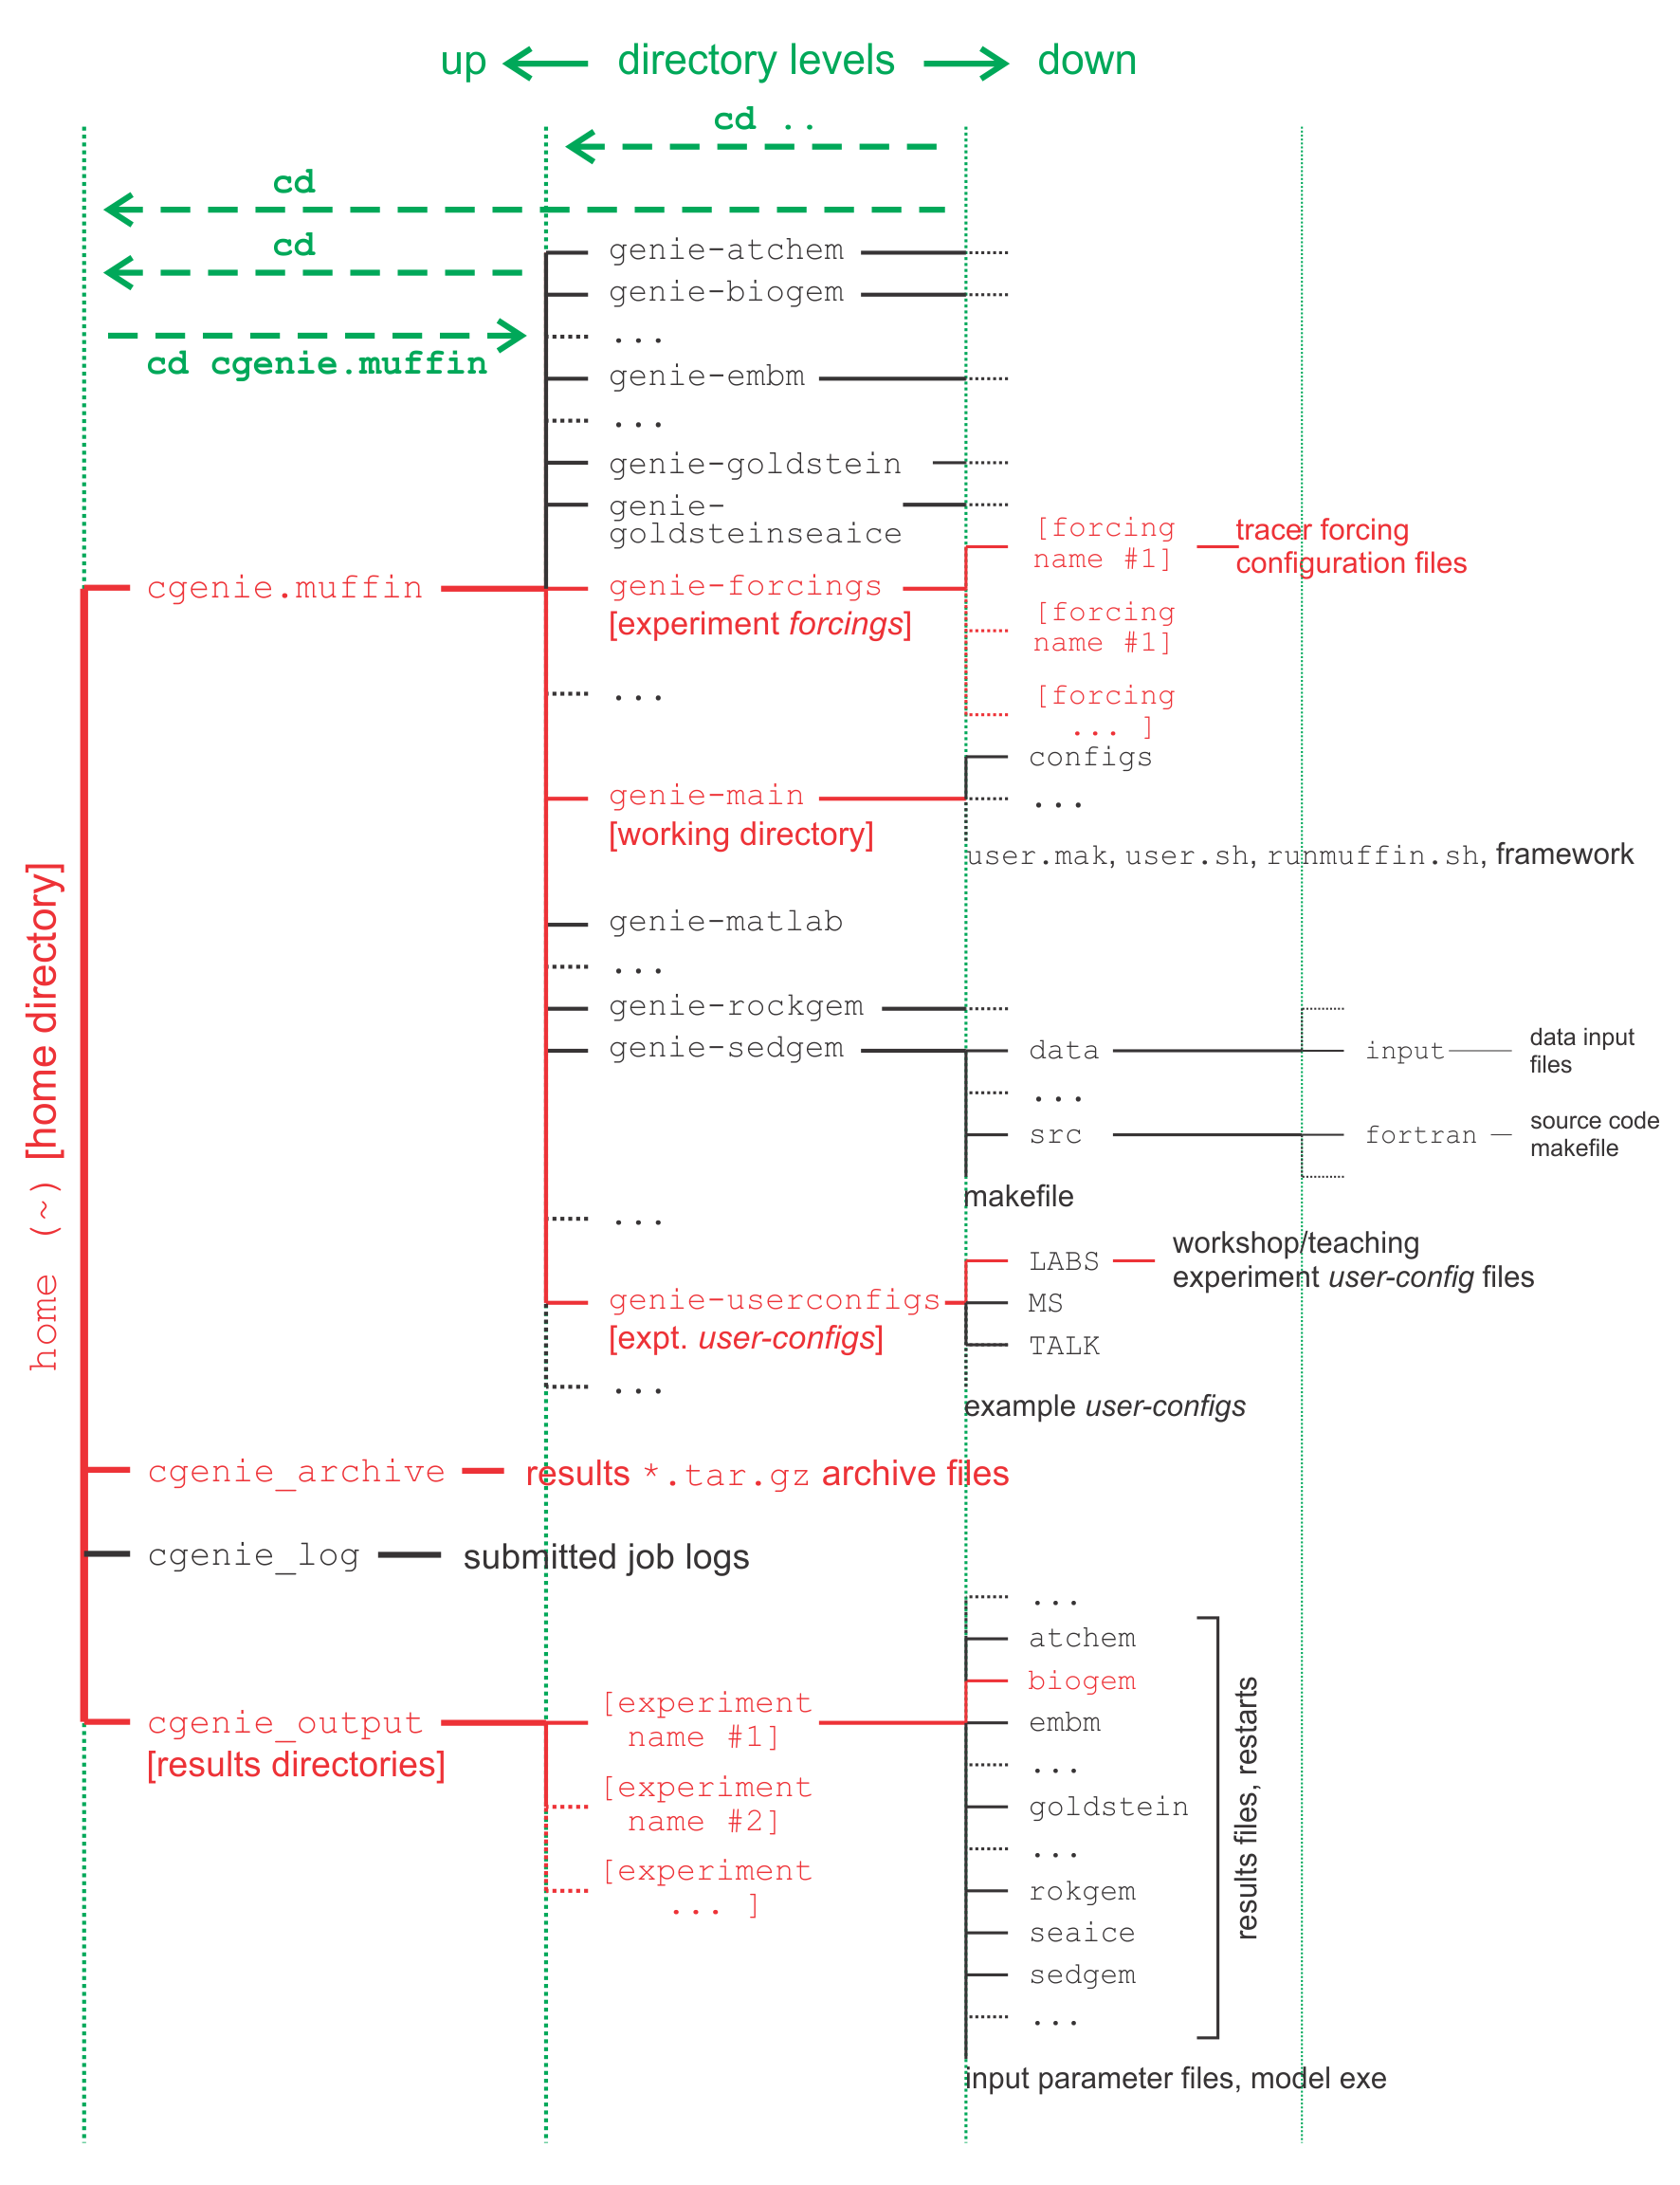
\includegraphics[width=\linewidth]{directories.png}
\caption{Directory structure of the \textbf{muffin} model. Highlighted in \textcolor{red}{red} are directories and sub-directories that you will need to access at some point. Vertical \textcolor[rgb]{0,0.501961,0}{green} lines designate directory levels, with example commands shown for moving between them.}
\label{fig:directories}
\end{figure}

%------------------------------------------------

\newpage

%------------------------------------------------

\section{Running the model}

The overall sequence of configuring and running \textbf{muffin} (job submission to a cluster queue), is shown in Figure \ref{fig:chx-jobcreation}. Refer to this if in any doubt at any point.

At the command-line (\texttt{\$}) in the \textsf{\footnotesize genie-main} directory (not your home directory), you will be entering in a command (\texttt{./runmuffin.sh}) together with a list of parameters that will be passed to the model, and as if by magic the model will run (or sometimes not). The form of the command you are going to be issuing is:

\vspace{-1mm}
\begin{verbatim}
$ ./runmuffin.sh #1 #2 #3 #4 (#5)
\end{verbatim}
\vspace{-1mm}

\noindent(\uline{don't type it yet}!)

\vspace{1mm}
The form of the command requires that you must list at least 4 parameters after \texttt{./runmuffin.sh}, separated by S P A C E S and on a single continuous line (even if it ‘wraps’ around across 2 lines of the screen).
These parameters are:

\vspace{2mm}
\begin{enumerate}[noitemsep]
\setlength{\itemindent}{.2in}
\item[\textbf{\#1}] ... is the name of the required base (or ‘basic’) configuration (‘\textit{base-config}’) of the model.
\item[\textbf{\#2}] ... is the name of the subdirectory (if any) containing the user configuration (‘\textit{user-config}’) file (i.e., the file containing the specification of a particular experiment).
\item[\textbf{\#3}] ... is the name of the experiment itself. There must exist a file in the directory specified by parameter \#2 (\texttt{LABS}) with exactly the same name as you enter here for parameter \#3 (i.e. parameter \#3 points to a file in the directory given by parameter \#2).
\item[\textbf{\#4}] ... is the run length of the experiment in years – this must be entered as an integer.
\item[\textbf{(\#5)}] ... There is also one optional (5th) parameter (described later).
\end{enumerate}



\vspace{1mm}
\noindent\rule{4cm}{0.1mm}
\vspace{2mm}

\noindent As an example of running the \textbf{muffin} Earth system model:

\vspace{2mm}
\begin{enumerate}[noitemsep]
\setlength{\itemindent}{.2in}
\item[\textbf{\#1}]: The base config is: \texttt{cgenie.eb\_go\_gs\_ac\_bg.worbe2.BASE}
\item[\textbf{\#2}]: The user config directory is: LABS
\item[\textbf{\#3}]: The user config file (the experiment name) is: \texttt{LAB\_0.EXAMPLE}.
\item[\textbf{\#4}]: Run the experiment for ten years: 10
\item[\textbf{\#5}]: (There is no restart file, and so no 5th parameter needs to be passed …)
\end{enumerate}

The full command for your first example experiment, which you are going to issue from the \texttt{\~}\texttt{/cgenie.muffin/genie-main} directory, then looks like:

\vspace{-1mm}
\begin{verbatim}
$ ./runmuffin.sh cgenie.eb_go_gs_ac_bg.worbe2.BASE LABS LAB_0.EXAMPLE 10
\end{verbatim}
\vspace{-1mm}

\noindent(\uline{you can try it now}!)

\vspace{2mm}
REMEMBER: This must be entered on a single CONTINUOUS LINE. The (single) S P A C E S are vital. Take care not to confuse an el (‘\texttt{l}’) with a one (‘\texttt{1}’) when typing this in ... (it is a ‘one’ here).

\vspace{1mm}
\noindent\rule{4cm}{0.1mm}
\vspace{2mm}

\noindent What should happen is: First, you will end up twiddling your thumbs a while, as all the components of \textbf{muffin} are compiled from the raw source code (\textbf{FORTRAN}). When it has finished doing this, the model will initialize and carry out some brief self-checking. Only then will it start actually ‘running’ and doing something, starting with a header describing the columns of numbers that follow:

\begin{itemize}
\item[] \texttt{model year}  -- ... guess!
\item[] \texttt{ice(\%)} -- global sea-ice fraction (\%)
\item[] \texttt{<SST>} -- global sea surface temperature ('SST') $^{\circ}$C
\item[] \texttt{<SSS>} -- global sea surface salinity ‘SSS’ (\%\textit{o})
\end{itemize}

The choice of what information to display on screen as the model is running is rather arbitrary, but the chosen metrics do tend to summarize some of the main properties of the climate system and carbon cycle – for my own personal convenience rather than reflecting any fundamental scientific truth ... you may also see columns of information for:

\begin{itemize}
\item[] p\(CO_{2}\)(uatm) -– mean atmospheric CO\(_{2}\) concentration (in units of \(\mu\)atm)
\item[] \(\delta^{13}CO_{2}\)  – mean \(\delta^{13}C\) value of atmospheric CO\(_{2}\) (\%\textit{o}) (NOTE: only if \(^{13}C\) tracer is selected)
\item[] \texttt{<DIC>} -- global mean ocean dissolved inorganic carbon (DIC) concentration (\(\mu\)mol kg-1)
\item[] \texttt{<ALK>}   – global mean ocean alkalinity (ALK) concentration (\(\mu\)eq kg-1) and in experiments with a modern continental configuration, also:
\item \texttt{AMO(Sv)} -- Atlantic meridional overturning circulation (Sv)
\\(and assuming that you have a modern continental configuration to even have an Atlantic ocean!)
\end{itemize}

This information is reported at the same intervals as time-series data (see later and/or refer to the User Manual) is saved and is indicated by:

\vspace{-2mm}
\begin{verbatim}
>>> SAVING BIOGEM TIME-SERIES AVERAGE CENTERED @ year :
\end{verbatim}
\vspace{-2mm}

Interleaved between these lines are lines reporting the saving of time-slice data (the 2- and 3-D model states – more of which later as well as in the User Manual). These appear as:

\vspace{-2mm}
\begin{verbatim}
>>> SAVING BIOGEM TIME-SLICE AVERAGE CENTERED @ year:
\end{verbatim}
\vspace{-2mm}

You can stop the model at any point (all data up to that time will have been saved) by hitting: \textsf{<Ctrl-C>} (\textsf{CONTROL} key + ‘\textsf{C}’ key).

Just from examining the screen output: how close to steady state does the system appear to have come after just 10 years? i.e., do SST and/or sea-ice extents appear to be converging towards stable (constant) values? This will be an important question to think about later on: ‘has the model reached steady-state (and does it matter)?’

In this particular example, the output should look something like the following:

\newpage

\footnotesize
\begin{verbatim}

 *******************************************************
 *** Initialisation complete: simulation starting ...
 *******************************************************

      model year  * pCO2(uatm)   d13CO2  *  AMO(Sv)  ice(%)   <SST>   <SSS>  *  <DIC>(uM)  <ALK>(uM)

 $N$        0.00       278.000   -6.500       0.000   0.000  -0.000  34.900      2244.000   2363.000
 >>> SAVING BIOGEM TIME-SLICE AVERAGE CENTERED @ year  :        0.500
 >>> SAVING BIOGEM TIME-SERIES AVERAGE CENTERED @ year :        0.500
 $N$        1.00       279.960   -6.598      13.613   0.744   2.509  34.901      2241.498   2363.111
 >>> SAVING BIOGEM TIME-SLICE AVERAGE CENTERED @ year  :        1.500
 >>> SAVING BIOGEM TIME-SERIES AVERAGE CENTERED @ year :        1.500
 $N$        2.00       279.525   -6.580      12.828   3.499   4.471  34.901      2240.173   2363.135
 >>> SAVING BIOGEM TIME-SERIES AVERAGE CENTERED @ year :        2.500
 $N$        3.00       279.258   -6.568      11.695   5.028   5.996  34.901      2239.169   2363.161
 >>> SAVING BIOGEM TIME-SERIES AVERAGE CENTERED @ year :        3.500
 $N$        4.00       279.044   -6.558      10.444   5.929   7.209  34.901      2238.354   2363.191
 >>> SAVING BIOGEM TIME-SLICE AVERAGE CENTERED @ year  :        4.500
 >>> SAVING BIOGEM TIME-SERIES AVERAGE CENTERED @ year :        4.500
 $N$        5.00       278.899   -6.551       9.380   6.191   8.156  34.902      2237.664   2363.220
 >>> SAVING BIOGEM TIME-SERIES AVERAGE CENTERED @ year :        5.500
 $N$        6.00       278.777   -6.545       8.500   6.623   8.975  34.902      2237.069   2363.246
 >>> SAVING BIOGEM TIME-SERIES AVERAGE CENTERED @ year :        6.500
 $N$        7.00       278.680   -6.541       7.922   6.629   9.637  34.903      2236.548   2363.267
 >>> SAVING BIOGEM TIME-SERIES AVERAGE CENTERED @ year :        7.500
 $N$        8.00       278.601   -6.537       7.917   6.738  10.225  34.903      2236.087   2363.285
 >>> SAVING BIOGEM TIME-SERIES AVERAGE CENTERED @ year :        8.500
 $N$        9.00       278.528   -6.534       7.952   6.740  10.732  34.904      2235.682   2363.301
 >>> SAVING BIOGEM TIME-SLICE AVERAGE CENTERED @ year  :        9.500
 >>> SAVING BIOGEM TIME-SERIES AVERAGE CENTERED @ year :        9.500
 $N$       10.00       278.466   -6.531       8.025   6.694  11.176  34.904      2235.325   2363.314

 *******************************************************
  *** Simulation complete: shutdown starting ...
 *******************************************************

\end{verbatim}
\normalsize

\begin{figure}
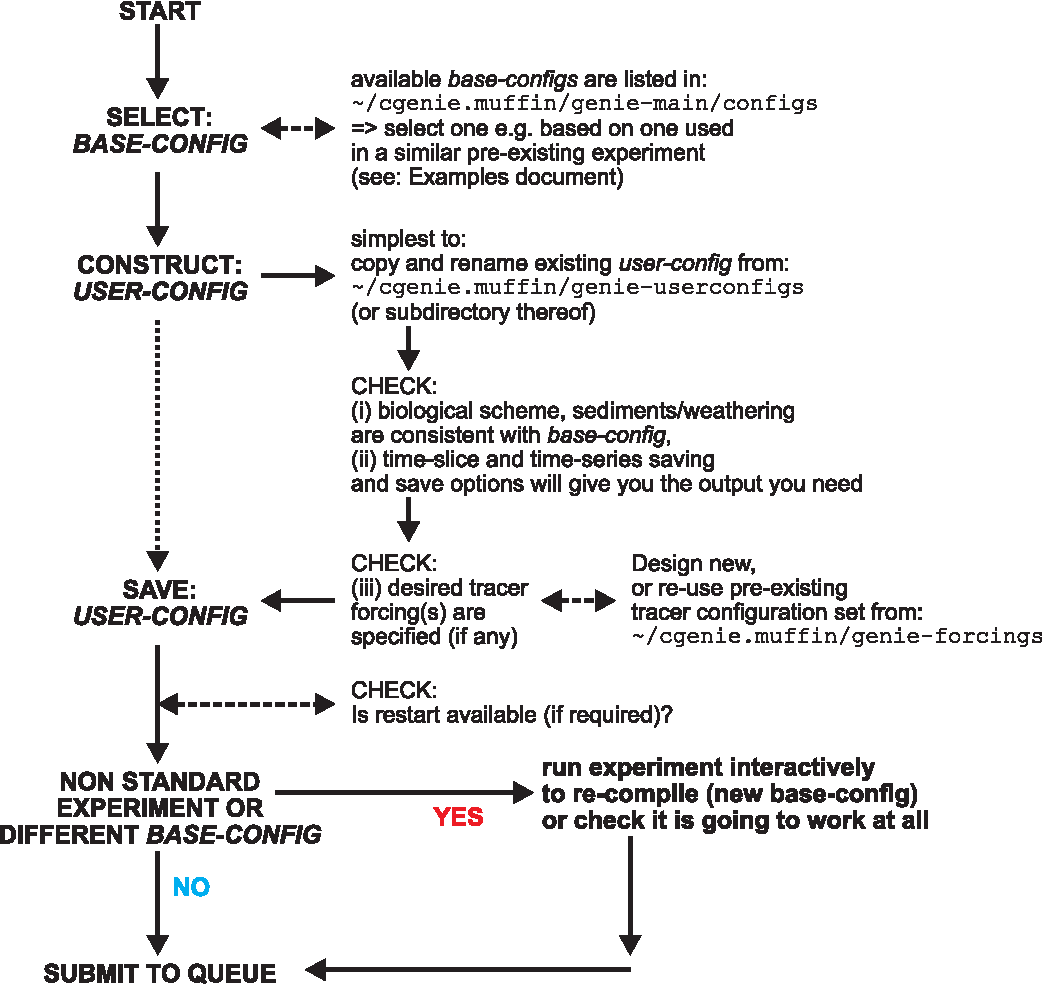
\includegraphics[width=0.9\textwidth]{chx-jobcreation.pdf}\centering
\vspace{-0mm}
\caption{Schematic of the sequence-of-events in configuring and running an experiment.}
\label{fig:chx-jobcreation}
\end{figure}

%------------------------------------------------

\newpage

%------------------------------------------------

\section{Creating new experiments!}

The key to creating new experiments is to remember that the name of the user-configuration file, that contains the parameter settings that define that specific experiment, becomes the name of the experiment and hence name of the model results sub-directory in \textsf{\footnotesize cgenie\_output}. Changing the name of the \textit{user-config} file, hence leads to a new experiment name and a new model results sub-directory. (Conversely, not changing the name of the  \textit{user-config} file and re-running it results in the results of any previous experiment run using that \textit{user-config} file, being over-written.)

There are two obvious ways to create a new \textit{user-config} file and hence new experiment (although the simplest and recommended way, is the 2nd one):

\begin{enumerate}[noitemsep]

\vspace{1mm}
\item Create a blank text file \footnote{\texttt{\$ touch file.txt} will achieve this at the linux command line.} and populate the contents with the parameter value assignments you need for your new experiment.
\\Inevitably, it is difficult to remember all the names and even values you want to specify, meaning that you'll end up looking at existing \textit{user-config} files and copying and pasting lines (or even the entire contents) from the old file(s) into your new \textit{user-config} file. So then you may was well ...

\vspace{1mm}
\item Copy and edit an existing file!
\\This is the most practical approach -- pick an existing \textit{user-config} file that is closest to the specific experiment that you want to run -- copy and rename it, then edit the contents and save. For the purpose of trying this out, you can literally pick on any existing file in the \textsf{\footnotesize LABS } subdirectory (of \textsf{\footnotesize genie-userconfigs}).
\\ You can do this by:
\begin{itemize}[noitemsep]
\item Using your sftp client (program):
\\First -- drag the existing \textit{user-config} file to your local computer. On your local computer, rename the file as per how you would 'normally' rename any file. 
\\Now you can edit the parameter values, re-save it, drag it back to the cluster (from your local computer) using the sftp client ... and finally run the experiment.
\item Or, if you are comfortable working at the linux command line; working from the same directory (e.g. \textsf{\footnotesize LABS}) that the file you want to copy lives in, you can copy a file (to a new filename) by:
\\\texttt{\$ cp oldfile newfile }
\\(after which you can edit the new \textit{user-config} file \textsf{\footnotesize newfile}, re-save, and then run the experiment.)
\end{itemize}
\vspace{1mm}

\end{enumerate}

\noindent Remember that the new \textit{user-config} file needs to be saved in (or copied to) the \textsf{\footnotesize genie-userconfigs/LABS} sub-directory (in the case of experiments carried out as part of the tutorials described in this manual), or anywhere else ... as long as you specify the correct path to the directory where you save the new file to\footnote{See previous Section and the use of the 2nd parameter passed to \texttt{runmuffin.sh}}.

%------------------------------------------------

\newpage

%------------------------------------------------

\section{Model output}

The first thing to note about output (i.e., saved results files) from \textbf{muffin} is that every science module saves its own results in its own sub-directory (and sometimes in very different and difficult-to-fathom ways …) – see Figure 1.1. All the sub-directories of results, plus copies of input parameters and the model executable, are gathered together in a directory that is assigned the same name as the experiment (== \textit{user-config} file name). The experiment results directories all live in:
\begin{verbatim}
~/cgenie_output
\end{verbatim}
and will be assigned a directory name something like:
\begin{verbatim}
LAB_0.EXAMPLE
\end{verbatim}
(this being the results directory name for an experiment called \texttt{LAB\_0.EXAMPLE}). Within this directory are each module’s results sub-directories.
We will primarily consider only results saved by the ocean biogeochemical module \textbf{‘BIOGEM’} (subdirectory: \small\texttt{biogem}\normalsize). The results files in this example will thus be found in:
\begin{verbatim}
~/cgenie_output/LAB_0.EXAMPLE/biogem
\end{verbatim}
\textbf{BIOGEM} has a flexible and powerful facility of saving results by means of spatially explicit ‘time-slices’, and as a semi-continuous ‘time-series’ of a single global (or otherwise representative mean) variable. In contrast, the atmospheric chemistry module '\textbf{ATCHEM}' does not save its own results (\textbf{BIOGEM} can save information about atmospheric composition and air-sea gas exchange) while the marine sediment module \textbf{SEDGEM} does save its own results, but only at the very end of a model experiment (\textbf{BIOGEM} can also save the spatial distribution of sediment composition as time-slices as well as mean composition as a time-series). Furthermore, to attain a common format for both ocean physical properties and biogeochemistry, \textbf{BIOGEM} can save a range of ocean results in addition to temperature and salinity, such as: velocities, sea-ice extent, mixed layer depth, convective frequency, etc.

\noindent NOTE: If in an sftp client window, you cannot 'see' the \textsf{\footnotesize cgenie\_output} directory, or cannot find any of the results sub-directories you are expecting, \uline{you will need to refresh the directory listing} (e.g. for \textbf{WinSCP}, there is a double green-arrow \textsf{\footnotesize Refresh} icon button near the top right of the window that you can click on). sftp client programs generally do not automatically refresh directory listing on the remote computer.

%------------------------------------------------

\subsection{Time-slice output}

One of the most informative data sets that can be saved is that of the spatial distribution of properties (such as tracers or physical ocean attributes). However, saving full spatial distributions (e.g., a 36\(\times\)36\(\times\)8 array) for any or all of the tracers each and every time-step is clearly not practical; not only in terms of data storage but also because of the detrimental effect that repeated file access has on model run-time.
Instead, \textbf{BIOGEM} will save the full spatial distribution of tracer properties only at one or more predefined time points (in units of years). These are termed \textit{time-slices}. At the specified time points, a set of spatially-explicit data fields are saved for all the key tracer, flux, and physical characteristics of the system. However, rather than taking an instantaneous snapshot, the time-slice is constructed as an average over a specified integration interval (the default is set to 1.0 years, i.e. an annual average). \textbf{BIOGEM}  assumes that the specified time point represents the mid-point of the (annual) average with the results that output years end up being reported as e.g.,
\begin{verbatim}
0.5
1.5
2.5
4.5
…
\end{verbatim}
(the mid-points of averages made over the intervals: 0-1, 1-2, 2-3, 4-5 years, etc.).

%------------------------------------------------

\subsection{Time-series output}

The second data format for model output is much more closely spaced in time. Model characteristics must then be reducible to a single meaningful variable for this to be practical (i.e., saving the time-varying nature of 3-D ocean tracer distributions is not). Suitable reduced indicators would be the total inventories in the ocean and/or atmosphere of various tracers (or equivalently, the mean global concentrations / partial pressures, respectively). Like the time-slices, the data values saved in the time-series files represent averages over a specified integration interval (the default is set to 1.0 years (annual average) but the results are reported with respect to the mid-point of the average which is where the ‘.5’ bits come in again).

%------------------------------------------------

\subsection{File naming convention}

The \textsf{\footnotesize biogem} results directory will contain files with names of the form:

\begin{itemize}[noitemsep]
\setlength{\itemindent}{.2in}
\item  \textsf{\footnotesize \_restart.nc} (is the re-start file created form the run you have just complete, and can be ignored).
\item \textsf{\footnotesize biogem\_series\_*.res} – these are the time-series files (in ASCII / plain text format).
\item \textsf{\footnotesize biogem\_year\_*\_diag\_GLOBAL.res} – these contain (global diagnostics) summary information and are saved at the same frequency as the time-slices (also as ASCII / plain text).
\item \textsf{\footnotesize fields\_biogem\_2d.nc} – 2-D fields of ocean and atmosphere properties, as NetCDF.
\item \textsf{\footnotesize fields\_biogem\_3d.nc} – 3-D fields of ocean properties, as NetCDF.
\end{itemize}

%------------------------------------------------

\newpage

%------------------------------------------------

\section{Viewing model output}

%------------------------------------------------

\subsection{Time-series output}

A descriptive summary of all the time-series (\texttt{biogem\_series\_*.res}) data files is given in the \textbf{muffin} User Manual if you are really that bored. The files of most immediate use/relevance are:

\begin{itemize}[noitemsep]
\setlength{\itemindent}{.2in}
\item \texttt{biogem\_series\_atm\_humidity.res}  - mean atmospheric (surface) humidity
\item \texttt{biogem\_series\_atm\_temp.res}      - mean atmospheric (surface) air temperature
\item \texttt{biogem\_series\_misc\_opsi.res}     - min/max overturning stream-function values (e.g. AMOC)
\item \texttt{biogem\_series\_misc\_seaice.res}   - mean ocean sea-ice cover and thickness
\item \texttt{biogem\_series\_ocn\_sal.res}       - mean ocean surface and whole ocean salinity
\item \texttt{biogem\_series\_ocn\_temp.res}      - mean ocean surface and whole ocean temperature
\end{itemize}

\vspace{1mm}
\noindent\rule{4cm}{0.1mm}
\vspace{2mm}

\noindent One way of viewing the contents of files is to change directory to the experiment results directory and opening the file in the file editor. But that is not so much fun.

Instead – change to the experiment results directory and then to the \textsf{\footnotesize biogem} sub-directory in the Secure File Transfer Client, and try double-clicking (if you have set up the \textbf{WinSCP} preferences correctly) or right-mouse-button-clicking (the then Edit with) on one of the .res files (listed above). For \texttt{biogem\_series\_ocn\_temp.res}, you should see 2 columns – time and mean (whole) ocean temperature ($^{\circ}$C). (However, in subsequent exercises a fuller output will be created with additional columns, with one for mean surface ocean temperature ‘SST’ ($^{\circ}$C) as well as mean benthic (bottom water) temperature ($^{\circ}$C)). Other results files may differ in the numbers of columns but all should be identifiable from the header information.

Note: \textbf{WinSCP} does not automatically refresh the directory listing. If you cannot see the results sub-directory with the experiment name you have just run, 99 times out of 100, it is because the display of the \textbf{WinSCP} needs to be refreshed -- there is an icon at the top of the program window or hit the ‘\textsf{F5}’ key.

\vspace{1mm}
\noindent\rule{4cm}{0.1mm}
\vspace{2mm}

\noindent For your information and edification (only): \textbf{Excel}, or \textbf{MUTLAB} if you prefer, can be used to graph the time-series results. Either way you will have to deal with the header line(s) that are present at the top of the file (and preceding the rows of data).

In \textbf{Excel}: Choose \textsf{\footnotesize File} then \textsf{\footnotesize Open}.  You will want to select \textsf{\footnotesize Files of Type} ‘\textsf{\footnotesize All Files (*.*)}’. In the \textsf{\footnotesize Text Import Wizard} window you can request that \textbf{Excel} skips the first few lines to start the import on the 2nd or 3rd line of the text file. Alternatively: set an appropriate column width manually in \textbf{Excel} to ensure that the columns of data are correctly imported.

\textbf{MUTLAB} will ignore lines starting with a \textsf{\footnotesize \%}, which the time-series starts with. However, it may be that the header line wraps-around and there is in effect a 2nd header line but without a \textsf{\footnotesize \%}. In this case, extra care (or a quick edit of the header in the ASCII file) will be required to load the data into \textbf{MUTLAB}.

%------------------------------------------------

\subsection{2- and 3-D time-slice output}

For the time-slice NetCDF (*.nc) files you will be using a program called \textbf{Panoply}. If you want your own (FREE!) copy of this utility, you can get it here (and is available for: \textbf{Windoz}, \textbf{Mac}, and linux operating systems): http://www.giss.nasa.gov/tools/panoply/.

\noindent When you open the NetCDF file, you will be presented with a ‘\textsf{\footnotesize Datasets and Variables}’ window (on the left hand side of the application window). This contains a list of all the parameters available that you can display. You will find that the ‘\textsf{\footnotesize Long Name}’ description of the variable will be the most helpful to identify the one you want. Simply double-click on a variable to display. 

For the 3-D fields you will be asked first whether you want a ‘\textsf{\footnotesize \footnotesize Longitude-Latitude}’ or ‘\textsf{\footnotesize Latitude-Vertical}’ plot (for the 2-D fields, the plot display will immediately open).
For the ‘\textsf{\footnotesize Longitude-Latitude}’ plots – there are multiple levels (depth layers) in the ocean - these data that can be plotted from the surface to the abyssal ocean. For the ‘\textsf{\footnotesize Latitude-Vertical}' plots – there are multiple possible longitudes at which to plot slices. The default is the global mean meridional distribution. There is also an option for ‘\textsf{\footnotesize Longitude-Vertical}' plots (which we will not use).

There may be multiple time-slices (i.e., you can plot data saved from different years). By default, only the very first \textit{time-slice} will be displayed.

You can choose interpolate the data or not (often you may find that it is clearer not to interpolate the data but to leave it as ‘blocky’ colors corresponding to the resolution of the model), change the scale and colors, overlay continental outline, change the projection, etc etc. Grey cells represent ‘dry’ grid points, i.e., continental or oceanic crust.

\vspace{1mm}
NOTE: The default settings in \textbf{Panoply} can mislead. Be aware of:
\vspace{1mm}
\begin{enumerate}
\item \textbf{Panoply} initially displays the very 1st time-slice (often year mid-point 0.5) time-slice rather than the experiment end. This can confuse and look like an experiment has not done anything!
\item By interpolating the data (not always misleading). To remove interpolation, un-tick:
\\‘\textsf{\footnotesize Interpolate}’ in the ‘\textsf{\footnotesize Arrays}’ tab.
\item By displaying a global zonal mean by default when selecting \textsf{\footnotesize Latitude-Vertical} plots. Then, to further confuse you, by plotting the output up-side-down (to invert: in the ‘\textsf{\footnotesize Grid}’ tab, hit ‘\textsf{\footnotesize Swap B/T}’ (for swap bottom/top).
\item By listing all ‘\textsf{\footnotesize Plottable variables}’ (option at the bottom of the window), when what you \textit{ideally} want are  the shorter and less confusing list of ‘\textsf{\footnotesize Georeferenced variables}’.
\item In \textsf{\footnotesize Longitude-Latitude} plots, by overlaying the modern continental output. (\textbf{muffin} land is marked in grey.)
\item By fitting a scale to the plot when the display window is opened, but not changing the scale when e.g., time or depth is changed. (The point of confusion is that you can quickly move outside the scale and end up with all model points dark blue or red.) Re-fit the scale, or manually set limited, in the ‘\textsf{\footnotesize Scale}’ tab.
So be careful when opening a new plot that you are looking at what you *think* you are looking at …
All the defaults can be changed via the ‘\textsf{\footnotesize Edit}’ drop-down menu and ‘\textsf{\footnotesize Preferences}’.
\end{enumerate}

\vspace{1mm}
\noindent\rule{4cm}{0.1mm}
\vspace{2mm}

\noindent Explore different data fields and play with different ways of displaying them. Aim for a set of display properties that show the information you are interested in / want to present in the clearest possible manner. Try different years (time-slice number), depth level (for a Latitude-Longitude plot), or longitude (for a vertical section).

\vspace{1mm}
\noindent\rule{4cm}{0.1mm}
\vspace{2mm}

\noindent To save plots in \textbf{Panoply}:
\small
\\\textsf{File}
\\\textsf{Save Image As …}
\normalsize
\\Then select the location, filename, and graphics format.

%------------------------------------------------

\newpage

%------------------------------------------------

\section{Submitting experiment ‘jobs’}

This bit is no particular fun at all, but it is a very handy ‘trick’ for running the model in the background, and maximizes drinking time in the bar vs. sat bored watching a computer screen :)

\vspace{1mm}
\noindent\rule{4cm}{0.1mm}
\vspace{2mm}

\noindent Running jobs interactively is all very well, but there are three important limitations:
\begin{enumerate}[noitemsep]
\vspace{1mm}
\item The connection between your terminal and the server computer running the model must remain unbroken. Anything more than a fleeting loss of internet connectively may result in the experiment terminating.
\vspace{1mm}
\item You can only run one experiment at a time … unless you want to have thousands of separate terminal open …? I thought not …
\vspace{1mm}
\item Any cluster or computer you are likely to be accessing using a shell will not have many computing cores itself, either because it is a single machine with only one or two processors, or if a cluster, by using a terminal you are running on the ‘head node’, which will have similar computing core limitations to running on a single machine. The more experiments you run simultaneously, the slower they will all run …
\end{enumerate}

\vspace{1mm}
\noindent\rule{4cm}{0.1mm}
\vspace{2mm}

\noindent The alternative is to submit your experiment as a ‘job’ to a queuing system which then manages what compute resources are used to run the model. Once you have submitted the experiment, that is it – you can go straight to the pub :)

For example -- to run the same experiment as before (\textsf{\footnotesize LAB\_0.EXAMPLE}) for maybe 100 years (or even longer if you wish – I am just pulling factors of 10 out of thin air here) but now submit the experiment as a job to the cluster queue, type:
\vspace{-1mm}
\small\begin{verbatim}
$ qsub -q dog.q -j y -o cgenie_log -V -S /bin/bash runmuffin.sh
  cgenie.eb_go_gs_ac_bg.worbe2.BASE LABS LAB_0.EXAMPLE 100
\end{verbatim}\normalsize
\vspace{-1mm}

\noindent(Again: SINGLE, CONTINUOUS LINE.) Here, the particular queue name is \textsf{\footnotesize dog.q}.

\vspace{1mm}
Note that now you should omit the ‘\texttt{./}’ bit before \texttt{runmuffin.sh}.
(If you are interested (I know that you are not): the options following \texttt{qsub} and before \texttt{runmuffin.sh} do things like re-directing screen output and error messaging to a file and specify which linux ‘shell’ to assume. It is even possible to receive an email when the job is done :) )
The status of the cluster queue and how you experiment job is getting on (e.g., “Is it finished yet?”) can be checked by typing:
\vspace{-1mm}
\small\begin{verbatim}
$ qstat -f
\end{verbatim}\normalsize
\vspace{-1mm}
(\texttt{qstat -f -u "*"} will show all jobs on the cluster.)

\vspace{1mm}
After submitting an experiment, you receive a job number. This number appears in the first column in the queue status information when you issue a qstat –f command. You should see your job appear on one of 6 compute nodes, numbered 0-0 to 0-5), although it might briefly reside as a ‘\textsf{\footnotesize PENDING JOB}’. For each node, there are multiple processing cores (depending on the specific cluster and queue), meaning that multiple instances of \textbf{muffin} can run simultaneously on each node. For an 8-level ocean based configuration of \textbf{muffin}, being run for 100 years, the job should remain there in the queue for a few minutes before ‘disappearing’ (your clue that it has finished, or died\footnote{If your experiment appears on the queue but vanishes after a few seconds, it has most likely died :(} …). If you periodically re-issue a \texttt{qstat –f} command you can follow your job’s progress.

\newpage 

A rough rule of thumb is that 8-level ocean \textbf{muffin} @ a horizontal grid resolution of 36x36 will simulate about 1000 years per CPU hour. The 16-level version (which you will use later), runs at about 300-400 years per CPU hour.

\noindent \textbf{NOTE}: It may be that the \textbf{FORTRAN} compiler is not accessible by the computer nodes. The implication of this is that \textit{the \textbf{muffin} executable must be already compiled BEFORE a job is submitted to the queue}.

\noindent In other words; if you have just changed the model resolution or continental configuration, or number of tracers (i.e. changed the \textit{base-config}) or issued a \texttt{make cleanall} command you MUST briefly run your desired experiment (or equivalent) interactively (i.e., in the shell window) to ensure that everything is correctly compiled. For instance, either run the experiment for a couple of years or start the experiment for the desired full duration, but 'kill it' (\textsf{\small Ctrl-C}) once the experiment is running successfully.

%------------------------------------------------

\newpage

%------------------------------------------------

\section{‘Restarts’}

Not much fun here either … but again – an important and time-saving (== increased drinking time!) modelling technique to learn to use.

By default, model experiments start from ‘cold’, i.e., the ocean is at rest and uniform in temperature and salinity while the atmosphere is uniform in temperature and humidity. All biogeochemical tracers in the ocean have uniform concentrations and/or are zero and there are no biogenic materials in deep-sea sediments. From this state it will take several thousand years (kyr) for the climate system to reach steady-state, and closer to 5 kyr (or more) for ocean biogeochemical cycles and atmosphere \(CO_{2}\) to reach steady-state, and exceeding 100 kyr for sediment composition to re-balance weathering ... Reaching this the equilibrium state is called the ‘\textit{spin-up}’ phase of the model.
There is evidently little point in repeating the \textit{spin-up} for each and every model experiment that are similar except in a single detail (e.g., testing a variety of different \(CO_{2}\) emissions scenarios all starting from current year 2012 conditions). A facility is thus provided for requesting that a ‘\textit{re-start}’ is used – starting a new experiment from the end of a previous one, usually a \textit{spin-up} that has been run explicitly for the purpose of generating a starting point (\textit{re-start}) of the system at steady-state (equilibrium) for subsequent experiments to continue on from.
It is important to note that there is nothing special about a \textit{re-start} – it is simply an experiment that you have already run. Equally, there is nothing special about the \textit{re-start}s you will download next – these you could have generated yourself – it simply saves time to have them provided.

\vspace{1mm}
\noindent\rule{4cm}{0.1mm}
\vspace{2mm}

\noindent To experiment with using a \textit{re-start}, you will first need to download a file that has been created (a pre-run 10,000 year spin-up). To fetch this: Change to the \textsf{\footnotesize cgenie\_output} directory (perhaps by going ‘home’ first (\texttt{cd} \textsf{\small <Enter>}), and then changing to \textsf{\footnotesize cgenie\_output} – refer to linux commands HOW-TO and Figure 1.1), and type:

\vspace{-2mm}
\begin{verbatim}
$ wget http://www.seao2.info/cgenie_output/LAB_0.SPIN.tar.gz
\end{verbatim}
\vspace{-2mm}

This downloads an archived/compressed copy of the restart from a location on the interweb. Extract the contents of this archive by typing:

\vspace{-2mm}
\begin{verbatim}
$ tar xfzv LAB_0.SPIN.tar.gz
\end{verbatim}
\vspace{-2mm}

Finally, change directory back to \textsf{\footnotesize cgenie.muffin} and then \textsf{\footnotesize genie-main} so that you are ready to run the model (the model is *always* run from the \textsf{\footnotesize cgenie.muffin/genie-main} directory).

\vspace{1mm}
\noindent\rule{4cm}{0.1mm}
\vspace{2mm}

\noindent A \textit{re-start} can be requested for  running on a new experiment from the end of a previous one, by providing a 5th   (optional) parameter when entering in the \texttt{runmuffin.sh} command. A spin-up of the modern World climate state is provided for you as a \textit{restart} -- \textsf{\footnotesize LAB\_0.SPIN} -- which you have just unpacked to the \texttt{cgenie\_output} results output directory.

To test out the use this \textit{restart} -- create a new (\textit{user-config}) experiment configuration file in the directory: 

\vspace{1mm}
\textsf{\footnotesize \(\sim\)/cgenie.muffin/genie-userconfigs/LABS}
\vspace{1mm}

\noindent taking the file \texttt{LAB\_0.EXAMPLE} (which is provided) as a template (no parameter changes need to be made yet). As described earlier -- copy this file and give it a new name -- here, name it: \textsf{\footnotesize LAB\_0.NEW}

\vspace{1mm}
You can then specify the use of the \textit{restart} in your new \textsf{\footnotesize LAB\_0.NEW} experiment:

\vspace{-2mm}
\small\begin{verbatim}
$ ./runmuffin.sh cgenie.eb_go_gs_ac_bg.worbe2.BASE LABS LAB_0.NEW 100 LAB_0.SPIN
\end{verbatim}\normalsize
\vspace{-2mm}

The run-time output should now look noticeably different. There should be no (or perhaps just very little) drift in any of the various variable values outputted to the screen – this is because you have (re-)started from the end of a run that had already ready an equilibrium, steady-state.

%----------------------------------------------------------------------------------------
%       CHAPTER 2
%----------------------------------------------------------------------------------------

\cleardoublepage

\chapterimage{Figure-1-The-image-of-an-ice-encased-Earth-a-Snowball-Earth-with-oases-of-open-water-on.png} % Chapter heading image

\chapter{Climate dynamics \& experimental design}\label{ch:climate-dynamics}

\hfill \break

\noindent Stuff to keep in mind:

\begin{itemize}
\vspace{1mm}
\item Models ARE NOT the ‘real World’ (it is going to be pretty obvious this is the case here).
\vspace{1mm}
\item Don’t believe what you read in Nature or Science.
\end{itemize}

%------------------------------------------------

\newpage

%------------------------------------------------

\section*{Readme}

You will need to download a new \textit{restart} file prior to embarking on the snowball Earth experiments.
To fetch this: change directory to the \textsf{\footnotesize cgenie\_output} directory, and type (or copy and paste carefully from this PDF ...):
\vspace{-2mm}
\begin{verbatim}
$ wget http://www.seao2.info/cgenie_output/LAB_1.SPIN.tar.gz
\end{verbatim}
\vspace{-2mm}

This downloads an archived/compressed copy of the experiment \textsf{\footnotesize LAB\_1.SPIN} – effectively, just an experiment (spin-up) that has already been run for 5,000 years for you. Extract the contents of this archive by typing (also from the \textsf{\footnotesize cgenie\_output} directory):
\vspace{-2mm}
\begin{verbatim}
$ tar xfzv LAB_1.SPIN.tar.gz
\end{verbatim}
\vspace{-2mm}

A new experiment results directly will then appear as if you had just run the entire 5,000 year experiment yourself (and you could in fact have done so). Reremember to refresh the \textbf{WinSCP} directory view window if you are using this particular software, or it might appear that nothing has been extracted.

You’ll then need to change directory back to \textsf{\footnotesize genie-main} to run the model.

\vspace{1mm}
If ... when you subsequently try and use this \textit{restart} in an experiment, \textbf{muffin} stops and complains that it cannot find it, check:
\begin{enumerate}[noitemsep]
\item That you in fact downloaded it to the correct directory, which should be: \textsf{\footnotesize cgenie\_output}, and not randomly to e.g. your home directory ...
\item That you unpacked it.
\end{enumerate}

%------------------------------------------------

\newpage

%------------------------------------------------

\section{Brrrrrrrrrrrr – it’s chilly on ... snowball Earth!}

To illustrate how ‘easy’ it can be to configure an Earth system / climate model such as \textbf{muffin} and explore the behavior of the Earth system and its response to perturbation – you are going to induce an extreme cooling of the climate system and see what happens. Solar output was weaker during the late Neoproterozoic, a time when the Earth experienced a series (2 ish) of extreme glaciations. Thus, having a mild climate state to start with must have been dependent on sufficient \(CO_{2}\) and/or \(CH_{4}\) in the atmosphere which presumably must have been highly elevated compared to the modern World ... sort of opposite to the problem we have today …

\vspace{1mm}
\noindent\rule{4cm}{0.5pt}
\vspace{2mm}

\noindent You are going to be running experiments in a similar manner to before, and using the \textit{re-start} experiment that you downloaded. You could then, for example, take the experiment configuration file \textsf{\footnotesize LAB\_1.EXAMPLE} (which is provided for you), and run the experiment, which has a new \textit{base-config}: \textsf{\footnotesize cgenie.eb\_go\_gs\_ac\_bg.woreq1.NONE}, by typing:
\vspace{-1mm}
\small\begin{verbatim}
$ ./runmuffin.sh cgenie.eb_go_gs_ac_bg.woreq1.NONE LABS LAB_1.EXAMPLE 100 LAB_1.SPIN
\end{verbatim}\normalsize
\noindent \uline{However} ... why not get into the habit of creating new and uniquely named experiments and their associated \textit{user-config} files (no harder than copying it and renaming it -- see earlier). If you keep using the same experiment name, the results will be over-written each time you re-run that experiment, whilst having  2 (or more) experiments running simultaneously with exactly the same name causes havoc as they try and over-write each others results files in a somewhat entertaining but ultimately useless way. So -- copy and rename the file \textsf{\footnotesize LAB\_1.EXAMPLE} to ... \textsf{\footnotesize LAB\_1.EXP1} or whatever (in the subdirectory \textsf{\footnotesize LABS}), and then run your newly created experiment:
\vspace{-1mm}
\small\begin{verbatim}
$ ./runmuffin.sh cgenie.eb_go_gs_ac_bg.woreq1.NONE LABS LAB_1.EXP1 100 LAB_1.SPIN
\end{verbatim}\normalsize

Remember that because you have changed since the exercises in the previous chapter, running the model first interactively (at the command line) is essential in order for the model code to be re-compiled consistent with the new configuration. i.e. you cannot directly start submitting experiments using the \textit{base-config} \textsf{\footnotesize cgenie.eb\_go\_gs\_ac\_bg.woreq1.NONE}, straight-away after having previous run the model using the \textsf{\footnotesize cgenie.eb\_go\_gs\_ac\_bg.worbe2.BASE} \textit{base-config}. Once you have re-compiled the model with the new \textit{base-config} and starting running (any experiment), you need not re-compile again and can submit as many jobs to the cluster queue as you like, up until you change \textit{base-config} once again.

\vspace{-1mm}
\noindent\rule{4cm}{0.5pt}
\vspace{2mm}

\noindent Overall: your task in this exercise will be to determine the radiative forcing (or p\(CO_{2}\) equivalent) threshold required to drive the climate system into a full ice-covered ocean (snowball Earth) state. (Read the \textit{Hyde et al.} [2000] paper.)

Useful 2-D (netCDF —- \textbf{Panoply}) variables to view are: surface air temperature and sea-ice extent (and/or thickness). Ocean surface temperature and salinity can be viewed in the 3-D NetCDF results file but are likely to be of less interest.

Time-series (ASCII \textsf{\footnotesize .res} files) are useful for providing simple mean indicators of global climate such as global ocean fractional sea-ice covered.

Note that the model configuration of an idealized super-continent you are using and as defined by the \textsf{\footnotesize cgenie.eb\_go\_gs\_ac\_bg.woreq1.NONE} \textit{base-config} file, positioned symmetrically about the Equator, is pretty unrealistic. But the further you go back in time, the more uncertain it becomes as to exactly where and in what orientation the continents were. Sometimes modelers have to resort to somewhat idealized experiments if the uncertainties are too great. In addition, one can conduct sensitivity experiments to test whether the continental configuration is important to the results. For instance, \textit{Hoffman and Schrag} [2002] discuss the potential importance of continental configuration, while the entire hypothesis of \textit{Donnadieu et al.} [2004] rests on specific details of the continental configuration being realistic.

For this configuration, the solar constant is set weaker than modern to reflect the fact that the Sun’s output has increased with time and during the Neoproterozoic the solar constant would have been ca. 5\% weaker. This is set by the model \textit{parameter}:

\vspace{-1mm}
\begin{verbatim}
ma_genie_solar_constant= 1285.92
\end{verbatim}
\vspace{-1mm}

\noindent which is set at the top of the provided \textit{user-config} file  \textsf{\footnotesize LAB\_1.EXAMPLE}. (For reference, the modern value is \( 1368 Wm^{-2}\).)

\vspace{1mm}
\noindent\rule{4cm}{0.5pt}
\vspace{2mm}

\noindent To search for the atmospheric \(CO_{2}\) concentration (or rather, radiative forcing equivalent) that would lead to a ‘snowball Earth’ state in the Neoproterozoic and answer the question:
‘How low does \(CO_{2}\) have to be to trigger a ‘snowball’?’
you are going to edit the experiment file that controls the specific details of the experiment -- the \textit{user-config} file. From the \textsf{\footnotesize genie-userconfigs/LABS} directory, open one of the snowball experiments in your preferred  text editor. At the top of the file you should see something like:

\vspace{-2mm}
\small\begin{verbatim}
#
#
# --- CLIMATE ---------------------------------------------------------
#
…
# scaling for atmospheric CO2 radiative forcing, relative to 278 ppm
ea_radfor_scl_co2=20.0
\end{verbatim}\normalsize
\vspace{-2mm}

Each line that is not commented out (i.e., no \#) contains a \textit{parameter} name and assigned value pair, with the format:
\vspace{-2mm}
\begin{verbatim}
PARAMETER=VALUE
\end{verbatim}
\vspace{-2mm}
The value of each parameter can be edited to change the experiment. (Additional parameter value specifications can also be added, or existing ones deleted.) In this example, the line:
\vspace{-2mm}
\begin{verbatim}
ea_radfor_scl_co2=20.0
\end{verbatim}
\vspace{-2mm}
specifies a radiative forcing of climate by \(CO_{2}\) equivalent to x20 modern (20x278 = 2560 ppm). If you instead wrote:
\vspace{-2mm}
\begin{verbatim}
ea_radfor_scl_co2=1.0
\end{verbatim}
\vspace{-2mm}
this would give you a modern\footnote{Technically: the pre-industrial \(CO_{2}\) value rather than ‘modern’ \textit{per se.}} (x1, or 1x278 = 278 ppm) radiative forcing.
Note: \(CO_{2}\) is not being explicitly modeled in this experiment, but the long-wave radiative forcing associated with a specified concentration of \(CO_{2}\) (in ratio to modern) is being set instead.

Edit the value of \texttt{ea\_radfor\_scl\_co2} (lower or higher -- your choice) and save the file (with a different filename!). Re-run the experiment until sea-ice extent starts to approach a new steady state. You may want to try  longer simulations than suggested (\textgreater 100 years) if it becomes clear that the model is still far from steady-state by the end of the experiment. You can judge how close to equilibrium things have got by following (and/or plotting) the evolution of e.g., global surface air temperature or sea-ice extent (both time-series files).

%\vspace{1mm}
%\noindent\rule{4cm}{0.5pt}
%\vspace{2mm}

\noindent 
In terms of methodology -- or; 'how am I going to answer the question' -- you will need to run mutilple different model experiments, each with a different value for the radiative forcing parameter, and find out for what value of the parameter, the Earth becomes completely ice-covered. It is your choice whether you change the radiative forcing parameter value, run the experiment, but wait for it to finish before deciding the radiative forcing parameter value to try for the next experiment -- i.e. a sequential approach, or try running multiple different 'guesses' simultaneously by submitting multiple different experiments to the queue. Ideally, each experiment will have a different name.

In each experiment, you want to be assessing how far towards the Equator the sea-ice limit encroaches by viewing some of the \textit{time-series} and \textit{time-slice} files or even the on-screen summary lines (assuming that you are running interactively rather than via a job submission to the cluster queue). Informative \textit{time-series} variables include (but are not necessarily be limited to): atmospheric temperature and sea-ice cover. (Sea-ice thickness, on account of the simple physics in the model, low resolution and long time-step, can fluctuate a little. This is also true for sea-ice area. Sea-ice volume is then the most reliable data (column) to keep track of in the \textit{time-series} output.)

For the \textit{time-slice} data: atmospheric and ocean surface temperature and particularly sea-ice extent (fractional cover), (2-D biogem \textbf{NetCDF} file) may be informative.

HINT: Be careful with the ‘\textsf{\footnotesize Fit to data}’ scaling feature in \textbf{Panoply} – at near complete sea-ice cover, you may find Panoply scaling min and max sea-ice between 99.1 and 99.9\% or something. Specific fixed scale limits (e.g. 0 and 100) can be set instead.

In answering the question (‘How low does \(CO_{2}\) have to be to trigger a ‘snowball’?’), think about what an appropriate degree of accuracy might be for your experiments. Just because computer models generally calculate to around 16 significant places of precision, does not mean you have 16 significant figures of realism. For instance – how many significant figures is the solar constant quoted to and what do you think is the uncertainty in this? Harder to judge is how the assumed (incorrect) continental configuration creates additional uncertainty, or the simple physics assumed in the ocean or sea-ice, or lack of snow on land …

\vspace{1mm}
Other questions to think about with regards to numerical modeling (as well as this particular experiment) are:

\begin{itemize}[noitemsep]
\setlength{\itemindent}{.2in}
\vspace{1mm}
\item  (Is the model configuration and experimental design ‘realistic’ ... ?)
\vspace{1mm}
\item  What is ‘missing’ in the model and what might the implications for your predictions and conclusions be? For example, there is no land-surface scheme (and hence no concept of ‘snow’) in this particular configuration.
\vspace{1mm}
\item Are the simulations being run for sufficiently long? Why not if not (i.e., justify your choices of parameter values and experimental assumptions)? How might the results and conclusions be biased (if at all)?
\vspace{1mm}
\item How would you test model predictions and your overall conclusions?
\vspace{1mm}
\item How could the experimental design be improved?
\end{itemize}

\vspace{1mm}
\noindent\rule{4cm}{0.5pt}
\vspace{2mm}

\noindent Once you are happy about the controls on the snowball threshold try and answer the supplementary question:

\vspace{2mm}
\noindent \textit{How high does the (\(CO_{2}\)) radiative forcing have to be in order to escape from a snowball?}
\vspace{2mm}

\noindent Having determined the appropriate radiative forcing value required to create a snowball state, you can use that experiment as a \textit{re-start}, and hence carry out a series of experiments with increasing radiative forcing, all starting from the same within-snowball climate state you have just created. Defining the radiative forcing / climate path going out of a snowball would complete the hysteresis loop of \textit{Hyde et al.} [2000]. 

Note that a good \textit{re-start} is one for which the experiment did not sit too long in the snowball state before finishing (the more sea-ice thickness you create in the first experiment, the more you are going to have to melt in the next and hence the longer this new series of experiments will take to ruin…). To achieve this, you can fine-tune the number of years the experiment is run, i.e. having determined the appropriate radiative forcing value required to create a snowball state, find out when (in terms of number of years) in the experiment the snowball state first occurred, and then run a new experiment that finishes only a decade or so after the snowball state was initiated.\footnote{You cannot select when the \textit{re-start} is saved – it is always saved at the end of an experiment.}

HINT: If you are having trouble deciding whether or not the snowball is heading in the right direction (i.e. towards an exit!), e.g. because sea-ice is always reported at 100\% (or close to), you can keep track of whether there is net melting or net freezing by following mean sea-ice thickness (m) as reported in the \textsf{\footnotesize biogem\_series\_misc\_seaice.res} time-series output file. Your indication of a melting snowball state is a progressive decline in mean thickness (a proxy for global ice volume). \uline{Note that you can open and review the results of \textit{time-series} files at *any* time during the experiment as the lines are written while the data for each time point is generated.}

Overall: think critically about the model configuration, the experimental design, and the nature of the scientific question (based on your background reading of snowball Earth). Some of the exploration/testing suggestions (above) may not necessarily give substantially different results. Such a finding would be as valid and interesting as determining an important dependence of a certain assumption, and would for instance indicate that the associated paleo uncertainties are not critical to model assessment of the question.

Always be prepared to justify all your choices for experimental design and model settings, e.g., range of radiative forcing assessed, continental configuration(s), solar forcing, use of re-starts (if any), run duration, etc. etc. etc. etc.

%------------------------------------------------

\newpage

%------------------------------------------------

\section{Further ideas}

%------------------------------------------------

\subsection{Feedback loop analysis}

To quantify the snowball Earth hysteresis loop in \textbf{muffin} as per Figure 2 in \textit{Hyde et al.} [2000] you will need to extract from the model ‘meaningful’ measures of climate (e.g., global surface air temperature, fractional sea-ice coverage) as a function of \(CO_{2}\) multiples, \(CO_{2}\) concentration, or (better) radiative forcing. For the latter, in \textbf{muffin}, the radiative forcing for a doubling of \(CO_{2}\) is set at: \(5.77 Wm^{-2}\). See: \textit{Myhre et al.} [1998] (Geophys. Res. Lett. 25, 2715–2718) and/or \textit{IPCC} [2007] for more on what radiative forcing is and how it is related to a relative change in \(CO_{2}\) concentration. Also, for making a comparison with \textit{Hyde et al.} [2000] -- for going into the snowball, note that they plot the change in radiative with a ‘cooling’ as positive (a bit daft). Their baseline radiative forcing state (an anomaly of \(0 Wm^{-2}\)) you might assume is equivalent to 278 ppm and hence \(\backsim\)130 ppm is an approximately halving of \(CO_{2}\) and hence creates \(\backsim5 Wm^{-2}\) of cooling. (You might prefer to plot the radiative forcing change as warming being positive, which makes rather more sense ...)

For coming out of a snowball, because the \(CO_{2}\) and hence radiative forcing threshold is so high as compared to going in, you may want to be creative in the plotting (assuming attempting to combine both thresholds into a single plot) and, for instance, one might break the scale between the low radiative forcing interval spanning going in and the high one spanning coming out.

Another example is as per Figures 3 and 4 in \textit{Stone and Yao} [2004] (Clim. Dyn. 22, 815–822) (although here it is the solar constant rather than long-wave radiation forcing that is being varied). So in fact, you could try varying the solar constant as an alternative to radiative forcing and hence be able to come up with a plot directly comparable to \textit{Stone and Yao} [2004].

%------------------------------------------------

\subsection{Continental configuration (1)}

It was mentioned earlier that the position of the continents is an area of modelling uncertainty and might be important. You can test for this. Four alternative \textit{base-configs} are provided, each defining a different continental configuration:

\vspace{1mm}
\begin{enumerate}[noitemsep]
\setlength{\itemindent}{.2in}
\item
\begin{verbatim}
cgenie.eb_go_gs_ac_bg.wopol1.NONE
\end{verbatim}
 – a single polar super-continent, with an ocean resolution of 36x36 with 8 vertical levels. (Note potential ‘l’ and 1’1 confusion in ‘\textsf{\footnotesize wopol1}’.)
\item
\begin{verbatim}
cgenie.eb_go_gs_ac_bg.wopol2.NONE
\end{verbatim}
  – one continent at each pole, with an ocean resolution of 36x36 with 8 vertical levels.
\item
\begin{verbatim}
cgenie.eb_go_gs_ac_bg.woreq1.NONE
\end{verbatim}
  – a single Equatorially-centred super-continent, with an ocean resolution of 36x36 with 8 vertical levels. [this is the current configuration (that you  used previously)]
\item
\begin{verbatim}
cgenie.eb_go_gs_ac_bg.woreq2.NONE
\end{verbatim}
 – two continents straddling the Equator, with an ocean resolution of 36x36 with 8 vertical levels.
\end{enumerate}
\vspace{1mm}

You can use the given \textit{user-config} file (\textsf{\footnotesize LAB\_1.EXAMPLE}) again as an experiment template file, and any of the alternative configurations can be run very similarly to as per before, i.e.:

\vspace{-2mm}
\begin{verbatim}
$ ./runmuffin.sh cgenie.eb_go_gs_ac_bg.xxxxx.NONE LABS LAB_1.EXAMPLE 100
\end{verbatim}
\vspace{-2mm}

Note that you are using a different \textit{base-config} file name: \textsf{\footnotesize cgenie.eb\_go\_gs\_ac\_bg.xxxxx.NONE}
\\where \textsf{\footnotesize xxxxx} is one of: \textsf{\footnotesize wopol1}, \textsf{\footnotesize wopol2}, \textsf{\footnotesize woreq1}, or \textsf{\footnotesize woreq2}.

\uline{Also note} that \uline{no} \textit{re-starts} are provided for any of these configurations. You may (or may not) want to create some (you will need to judge for yourselves how long to run the \textit{re-start} experiments for to achieve as close to steady-state as you think is ‘sufficient’). Recall again, that \textit{re-starts} are just ‘normal’ experiments that have already been run.
Be careful that when changing from one \textit{base-config} to another, the model re-compiles. Simply running the new configuration briefly (for even just a single year) is sufficient to ensure this. Experiments can then be safely submitted to a cluster queue, i.e. do not try and submit an experiment using a different \textit{base-config} straight to the cluster queue without having run it (or a short version of the experiment you want) interactively first (to ensure the model is re-compiled). This is also good practice – checking that a new sort of experiment and/or model configuration works as you intend and without hiccups.

%------------------------------------------------

\subsection{Continental configuration (2)}

Although much useful can be learned from conceptual configurations and Worlds regarding climate dynamics, it is invariably aesthetically more 'pleasing' to also test ideas in a more paleogeographically realistic configuration. Provided is a set of \textit{base-config} and \textit{user-config} files (plus associated boundary conditions) for the position of the continents and climate 635 millions years ago (635 Ma). For this:

\vspace{1mm}
The \textit{base-config} is named: \textsf{\footnotesize muffin.C.fm0635cb.NONE}

\vspace{1mm}
The \textit{user-config} is: \textsf{\footnotesize muffin.C.fm0635cb.NONE.SPIN}

\vspace{1mm}
NOTE that the \textit{user-config} lives in the directory: \textsf{\footnotesize \(\sim\) \textbackslash cgenie.muffin\textbackslash user-configs\textbackslash PALEO}

\noindent so that you either need to specify this different (\textsf{\footnotesize PALEO}) directory when running \textbf{muffin}, or copy the \textit{user-config} file into \textsf{\footnotesize LABS}.

\vspace{1mm}
A \textit{re-start }experiment is provided called \textsf{\footnotesize muffin.CB.fm0635cb.NONE.SPIN} and which can be downloaded as per before:

\vspace{-2mm}
\begin{verbatim}
$ wget http://www.seao2.info/cgenie_output/muffin.CB.fm0635cb.NONE.SPIN.tar.gz
\end{verbatim}
\vspace{-2mm}

\noindent and unpacked by:

\vspace{-2mm}
\begin{verbatim}
$ tar xfzv muffin.CB.fm0635cb.NONE.SPIN.tar.gz
\end{verbatim}
\vspace{-2mm}

\noindent (Remember: you should be in the \textsf{\footnotesize cgenie\_output} directory when you do this downloading and unpacking.)

To run (e.g. for 100 years), following on from its \textit{re-start} (and leaving the \textit{user-config} in its \textsf{\footnotesize PALEO} directory):

\vspace{-2mm}
\begin{verbatim}
$ ./runmuffin.sh muffin.C.fm0635cb.NONE PALEO muffin.C.fm0635cb.NONE.SPIN
    100 muffin.CB.fm0635cb.NONE.SPIN
\end{verbatim}
\vspace{-2mm}

\noindent (\uline{all on one line})\footnote{NOTE that the \textit{base-config} and \textit{user-config} filenames start \textsf{\footnotesize muffin.C.} whereas the\textit{ re-start} filename starts \textsf{\footnotesize muffin.CB.} ... just to try and trip you up ...}

\vspace{1mm}

%------------------------------------------------

\subsection{Geothermal heat input}

Finally, \textbf{muffin} will fairly happily build up sea-ice, apparently without limit (with the remaining wet ocean becoming progressively colder and more saline). In the real world, one might expect some sort of limit to the maximum thickness achieved as the heat diffusion across a progressively greater thickness of sea-ice approaches the heat input at the bottom of the ocean from geothermal energy. Different modes of ocean circulation are also possible if one considers heating from the bottom as well as cooling (and brine rejection) from the top and which might affect the entry into or exit from a snowball state.

In the experimental setup you have been given, a geothermal heat input is specified in the ocean circulation module via the following :

\vspace{-2mm}
\begin{verbatim}
bg_ctrl_force_GOLDSTEInTS=.TRUE.
bg_par_Fgeothermal=100.0E-3
\end{verbatim}
\vspace{-2mm}

The parameter \textsf{\footnotesize bg\_par\_Fgeothermal} sets the geothermal flux in units of W m$^{-2}$. (Note that in the Neoproterozoic, the geothermal heat flux could have been somewhat higher than modern. How much higher? A question for \textbf{Google} … ?)

An appropriate research question might be to determine in radiative forcing \textit{vs.} geothermal space (and requiring a 2D grid of parameter combinations to be created and submitted to the cluster), the equilibrium sea-ice thickness and region in which a snowball solution is not possible. However, more simply and suitable to a short exercise: How much of a difference, to the estimated snowball entry and exit thresholds of radiative forcing, does the inclusion of a geothermal input make? E.g., what happens if you set it to zero? What about 10 times modern (or more, although *extreme* seafloor heating can cause numerical instability and the model to crash)?

%------------------------------------------------

\subsection{Seasonality}

By default, the idealized model configurations are non-seasonally forced (by solar insolation). You can switch to a seasonally-forced to model by adding the following lines to the \textit{user-config} file:

\vspace{-3mm}
\begin{verbatim}
ea_dosc=.true.
go_dosc=.true.
gs_dosc=.true.
\end{verbatim}
\vspace{-2mm}

The scientific question here in trying this would be whether or not taking into account a seasonally-varying climate substantially affects the entry (and/or exit) thresholds for a snowball climate state. (At least, whether it is important in the context of the resolution and physics of the model you are using.)

You can also save the data seasonally if you like – see Section 12.2.3 in the \textbf{muffin} User Manual (this document!).\footnote{For reference, your configuration has 24 time-steps per year set for the \textbf{BIOGEM} module.}

%----------------------------------------------------------------------------------------
%       CHAPTER 3
%----------------------------------------------------------------------------------------

\cleardoublepage

\chapterimage{amoc.png} % Chapter heading image

\chapter{Ocean circulation}\label{ch:ocean-circulation}

\hfill \break

\noindent Stuff to keep in mind:

\begin{itemize}
\item Nothing at all – keep your mind completely empty and let the wonderful truths of \textbf{muffin} permeate your entire being.
\end{itemize}

\vspace{2mm}
\noindent Background reading (Atlantic circulation and stability in \textbf{muffin}):

\vspace{2mm}
\begin{itemize}
\item Hargreaves et al. [2004] (Climate Dynamics 23, 2004, Pages 745 – 760)
\\\(\rightarrow\)Simple assessment of the likelihood of AMOC collapse.
\item Marsh et al. [2004] (Climate Dynamics, 23 2004, Pages 761 – 777)
\\\(\rightarrow\)Characterization of thresholds of AMOC collapse.
\item Singaraye et al. [2008] (GRL 35, doi:10.1029/2008GL034074)
\\\(\rightarrow\)Role of changing ocean circulation in atmospheric radiocarbon variability during the Younger Dryas.
\end{itemize}

\vspace{2mm}
\noindent Background reading (Miscellaneous (model) Atlantic circulation and stability):

\vspace{2mm}
\begin{itemize}
\item Rahmstorf et al. [2006] (In: Encyclopedia of Quaternary Sciences, Edited by S. A. Elias. Elsevier, Amsterdam)
\\\(\rightarrow\)Provides the background to the Atlantic Meridional Overturning Circulation and hypothesized hysteresis.
\item IPCC [2007] (e.g., Section 10.3.4)
\\\(\rightarrow\)Future predictions of AMOC strength.
\item Schmittner [2005] (Nature 434, 628– 633)
\\\(\rightarrow\)Impacts on marine ecosystems and carbon cycling.
\item Obata [2007] (J. Clim. 20, 5962–5976)
\\\(\rightarrow\)Climate-carbon cycle model response to freshwater discharge.
\end{itemize}

%------------------------------------------------

\newpage

%------------------------------------------------

\section*{READ.ME}

You will need to download a new \textit{re-start} file prior to embarking on the experiments with modern ocean circulation.
To fetch this: change to the \texttt{cgenie\_output} directory, and type (or copy and paste carefully from the PDF ...):

\vspace{-2mm}
\begin{verbatim}
$ wget http://www.seao2.info/cgenie_output/LAB_2.SPIN.tar.gz
\end{verbatim}
\vspace{-2mm}

This downloads an archived/compressed copy of the 10,000 year \textit{spin-up} experiment \texttt{LAB\_2.SPIN}. Extract the contents of this archive by typing:

\vspace{-2mm}
\begin{verbatim}
$ tar xfzv LAB_2.SPIN.tar.gz
\end{verbatim}
\vspace{-2mm}

You’ll then need to change directory back to \texttt{genie-main} to run the model.

%------------------------------------------------

\newpage

%------------------------------------------------

\section{Tracing ocean circulation}

The ocean biogeochemistry module (\textbf{BIOGEM}) in \textbf{muffin} provides a framework for applying time- and spatially-variable ‘forcings’ of the Earth system\footnote{Refer to the '\textit{force the system}' \textsf{HOW-TO} in the muffin manual for further details on \textit{forcings}.} – fluxes or restored-to boundary conditions that can be prescribed for any gas, dissolved substance (including temperature and salinity), or particulate matter. Examples include freshwater input (== a negative salinity flux forcing) of the North Atlantic to alter ocean circulation, fossil fuel \(CO_{2}\) emissions to the atmosphere (== a \(CO_{2}\) gas flux forcing), or aeolian iron supply to the surface ocean (a 2-D dust flux forcing).

For example: view the \textit{user-config} file: \textsf{\footnotesize LAB\_2.colorinjection} – you will see the following lines (under the heading: ‘\texttt{\# --- FORCINGS ---}’)

\vspace{-2mm}
\begin{verbatim}
bg_par_forcing_name="pyyyyz_Fred"
bg_par_force_point_i=22
bg_par_force_point_j=33
bg_par_force_point_k=8
bg_par_ocn_force_scale_val_48=0.0
\end{verbatim}
\vspace{-2mm}

The first line points \textbf{muffin} to a directory located in \textsf{\footnotesize cgenie.muffin/genie-forcings} that contains a set of files that define what geochemical property is going to be altered plus information about how the magnitude of the forcing changes with time.

There are then three lines (\texttt{bg\_par\_force\_point\_i=20}, ...) that specify the location in the ocean of the geochemical forcing that is going to be applied. The point sources are specified in (i,j,k) coordinates, which in this case is (22,33,08). For the ocean model resolution we are using, the grid is 36x36x16, and in which: longitude (i) is counted from left-to-right (1 to 36); latitude (j) is counted from bottom-to-top (1 to 36); level depth (k) is counted from downwards top-to-bottom (16 down to 1). Thus, (22,33,08) is a release of tracer in the North Atlantic, a little south of Greenland, and intermediate depth (level = 8 out of 16). Refer to the Figures for how the horizontal (Figure \ref{fig:ch3-ijgrid}) and vertical (Figure \ref{fig:ch3-kgrid}) grid is specified.

Finally, there is a scaling parameter (\texttt{bg\_par\_ocn\_force\_scale\_val\_48}) which modifies the magnitude of the flux to be applied (in units of \(mol yr^{-1}\)).

\begin{figure}
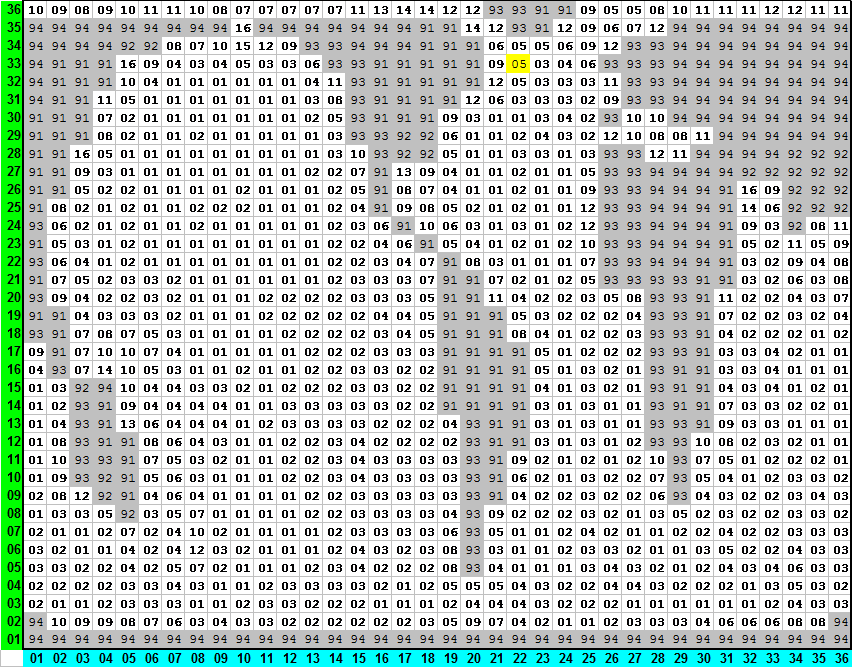
\includegraphics[width=0.8\textwidth]{ch3-ijgrid.png}\centering
\vspace{-0mm}
\caption{
\textbf{The  muffin grid for a modern \(36\times36\) ‘worjh2’ configuration.} Light blue numbers are the ‘i’ co-ordinates. Green numbers are the ‘j’ co-ordinates.
The depth of the ocean at any location is indicated by its ‘k’ value – a number between 1 and 16, with 16 being the surface layer of the ocean, and 1 the maximum possible depth anywhere.
Numbers > 90 (91, 92, 93, 94) and shaded grey are land (and specify the direction of run-off).
Location (22,33,08) is highlighted in yellow.
The longitude of the western edge of this particular modern ocean grid is at 260W, and the increments are 10 degrees.
}
\label{fig:ch3-ijgrid}
\end{figure}

\begin{figure}
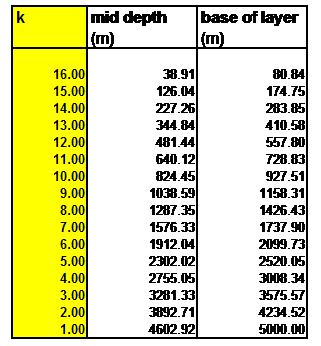
\includegraphics[width=0.4\textwidth]{ch3-kgrid.png}\centering
\vspace{-0mm}
\caption{\textbf{The muffin ocean vertical level definitions for a modern 16-level ocean grid.}}
\label{fig:ch3-kgrid}
\end{figure}

\vspace{1mm}
\noindent\rule{4cm}{0.5pt}
\vspace{2mm}

\noindent You are going to run a brief experiment in which you will be injecting a conservative ‘dye’ tracer into the ocean. The \textbf{BIOGEM} module has two tracers defined for this purpose – ‘blue’ and ‘red’. Open the \textit{user-config} file: \textsf{\footnotesize LAB\_2.colorinjection} and edit the parameter controlling the flux of red dye to read:

\vspace{-2mm}
\begin{verbatim}
bg_par_ocn_force_scale_val_48=1.0E12
\end{verbatim}
\vspace{-2mm}

\noindent which specifies a flux of \(1.0\times10^{12}\) ( \(mol yr^{-1}\)) rather than zero as given as the default in the example \textit{user-config} file\footnote{i.e. don't leave the value as zero ... otherwise you'll have no flux forcing applied and will not see anything happen ...}.

The \textit{base-config} you will be using is different from previously: \textsf{\footnotesize cgenie.eb\_go\_gs\_ac\_bg.worjh2.rb} – this specifies a 16 vertical levels ocean and also includes seasonality of solar insolation.

\vspace{1mm}
\noindent\rule{4cm}{0.5pt}
\vspace{2mm}

\newpage 

\noindent Run the model for … whatever, 20 years will do. Use the \textit{re-start} experiment that you have just downloaded to start from:

\vspace{-2mm}
\begin{verbatim}
$ ./runmuffin.sh cgenie.eb_go_gs_ac_bg.worjh2.rb LABS
  LAB_2.colorinjection 20 LAB_2.SPIN
\end{verbatim}
\vspace{-2mm}

View the results – for instance how the red tracer distribution evolves with time – in the \textit{time-slice} files (full ocean/atmosphere) properties saved in the \textbf{netCDF} format (\texttt{.nc}) files). You can follow the progress of the dye (and hence diagnose the properties of ocean circulation in the model) by plotting vertical and/or horizontal slices that go through (or near) the cell location in which you inject the dye tracer in the 3D \textbf{netCDF} file. Note that \textbf{Panoply} appears to ‘count’ the ocean layers in the opposite direction to the way in which the ocean model is actually counting them – the correct definition is with ‘1’ being very deepest level possible (and as displayed in the figure).

You can also view the tracer distributions in terms of a water-column integrated tracer inventory (\textbf{netCDF} variable name: \textsf{\footnotesize ocn\_int\_colr}; long name: \textsf{\footnotesize colr water-column integrated tracer inventory}) in the 2D \textbf{netCDF} output. (See: \textit{Sabine et al.} [2004] for the use of water column integrals in the context of the distribution of anthropogenic \(CO_{2}\) uptake and storage.) Changes in tracer inventory with time can be tracked in the time-series file
\vspace{-2mm}
\begin{verbatim}
biogem_series_ocn_colr.res.
\end{verbatim}
\vspace{-2mm}

You can also plot the overturning circulation from the 2D netCDF file – variable phys\_opsi == global overturning streamfunction, \textsf{\footnotesize phys\_opsia} == overturning in the Atlantic to provide a visualization of the large-scale ocean circulation that drives tracer movement.

Spend a little while altering the flux (\texttt{bg\_par\_ocn\_force\_scale\_val\_48}) and/or location (\texttt{bg\_par\_force\_point\_i}, \texttt{bg\_par\_force\_point\_j, bg\_par\_force\_point\_k}) of tracer input. Overall -- note how you can use numerical ‘tracers’ to help diagnose (and better understand) the circulation of the ocean.

\vspace{1mm}
\noindent\rule{4cm}{0.5pt}
\vspace{2mm}

\noindent When you add the numerical dye, particularly early on in the experiment, you may see a 'front' of \uline{negative} tracer concentrations leading the (positive) tracer as it spreads. DON'T PANIC!

The model is ... a model (of the numerical flavor) and not an exact analytical solution. So errors in how it solves ocean transport are to be expected.

Moreover, by default the ocean circulation model employs an isopycnal/diapycnal mixing scheme. This can lead to unwanted negative tracer values when sharp horizontal (or vertical) transitions in concentration occur. (In this example, e.g. by injection dye at a point location into a surrounding ocean of initially zero concentration.)

You can change to a simpler horizontal/vertical (.false.) mixing scheme by adding to the \textit{user-config} file:
\vspace{-2mm}
\begin{verbatim}
# turn OFF (=.false.) isopycnal/diapycnal mixing
go_diso=.false.
\end{verbatim}
\vspace{-2mm}

If you try this, you should (hopefully) find much less (or no) negative tracer concentrations occur. However, also note that by changing the physics of ocean mixing, you also slightly alter the large-scale circulation of the ocean (and e.g. the AMOC might change slightly in strength).

\vspace{1mm}
\noindent\rule{4cm}{0.5pt}
\vspace{2mm}

\noindent Finally, an interesting (honest!) and illustrative exercise is to use the dye tracer to pick out the path taken by Mediterranean Intermediate Water. Despite the low resolution of the \textbf{muffin} ocean circulation model component and the highly restricted representation of the Mediterranean, the model does predict a salty Mediterranean as a consequence of P-E in this basin (and its catchments) being negative and this water makes its way out in the subsurface into the Atlantic.

Simply specify a dye injection somewhere in the Mediterranean (be careful with the restricted depth of the Mediterranean – if you inject too deeply (into the crust!) then you will not see anything (refer to the figure for the depth level (k) number of the maximum depth of the water column in each location), and it is better to inject it relatively close to the opening of the gateway (try some different locations and see which ones produce a reasonably instructive tracing of Mediterranean outflow). Run for e.g., 20 or 50 years (from the provided spin-up). Then:

\vspace{1mm}
\begin{enumerate}[noitemsep]
\vspace{1mm}
\item View the dye-tagged plume of Mediterranean Intermediate Water by plotting a lat-lon slice (from the 3D \textbf{netCDF} file). This will give you the depth of the plume. How does this compare with salinity observations (salinity observations and appropriate global datasets can be found on the web with a little patience)? You can also view the water-column integrated distribution (2D \textbf{netCDF}).
\vspace{1mm}
\item Try viewing the plume via a lat-depth slice. Refer to the figure to determine the ‘i’ value up the Atlantic that will just graze the edge of what passes for Spain at this low model resolution. Which direction does it head after exiting the Mediterranean? Is this ‘realistic’?
\end{enumerate}
\vspace{1mm}

%------------------------------------------------

\newpage

%------------------------------------------------

\section{Poking the climate beast}

Instead of adding a dye tracer, you could add fresh water to the ocean surface to assess the sensitivity of the Atlantic Meridional Overturning Circulation (AMOC) to collapse, in a classic ‘hosing’ experiment.

The \textit{user-config} file for this is called: \texttt{LAB.2.hosing}. The default (i,j) location of the flux input is the same (as the dye tracer), but now the injection at the surface (level: k=16). Note that the forcing of the salinity tracer is negative (freshwater = negative salinity compared to sea-water)!

To orientate you in freshwater forcing space: \texttt{bg\_par\_ocn\_force\_scale\_val\_2=-2.0E17} should be sufficient to make ‘stuff happen’ and quickly. BUT, this is a pretty extreme flux (see overleaf for a rough conversion between salinity forcing units (mol yr$^{-1}$) and fresh water flux (in m$^{3}$ s$^{-1}$ or Sv). Much more than this and the model may crash or at the very least, you’ll be left with a large freshwater pond in the North Atlantic … (See later (Section 1.6e) for some exciting discussion on units!)

To run the model for e.g., 20 years using the same restart:

\vspace{-2mm}
\begin{verbatim}
$ ./runmuffin.sh cgenie.eb_go_gs_ac_bg.worjh2.rb LABS
  LAB_2.hosing 20 LAB_2.SPIN
\end{verbatim}
\vspace{-2mm}

\noindent 20 years should be long enough to see a collapse start to occur, but you might want to run the model for longer (and it can be submitted as a job, of course). Running for longer will also allow you to have a smaller, less extreme (and maybe more realistic) freshwater input flux.

The most obvious property of the Earth system to follow is the Atlantic overturning strength (\textsf{\footnotesize biogem\_series\_misc\_opsi.res}). The AMOC stream-function (in \textsf{\footnotesize fields\_biogem\_2d.nc} 2-D time-slice \textbf{netCDF} results file, field: \textsf{\footnotesize phys\_opsia}) is also illustrative. You can also try and identify the salinity anomaly (see below) due to freshwater input in the 3D salinity tracer field.

There are also important (but not necessarily painfully exciting) impacts on surface air temperatures and maybe sea-ice extent (in \texttt{fields\_biogem\_2d.nc)} (but see below for a better way to visualize these changes). Note the importance (sort of) of the AMOC in transporting heat to the N Atlantic region (the film the Day After Tomorrow was not entirely inaccurate in this particular respect). Be aware of the possibility of climate impacts far from the location of fresh water forcing. Look out for any significant-looking impacts on sea-ice extent, etc.

Note that as the model is running rather s l o w e r than in the snowball configuration, you might want to think carefully of making use of cluster queuing possibilities (i.e., running multiple experiments at once in the background).

Also -- run a \uline{control} experiment -- an experiment of the same duration of your hosing experiments, but with a zero freshwater flux. The impact of freshwater input, is the difference, at the same model year, between the perturbation experiment and the control. (You only ever need need to run one control, regardless of how many different freshwater flux perturbation experiments  you run.) 

\vspace{1mm}
\noindent\rule{4cm}{0.5pt}
\vspace{2mm}

\noindent To more easily assess some of these impacts (and for other sorts of analysis) it is possible to create an \uline{anomaly (difference) map} in \textbf{Panoply}:

\vspace{1mm}
\begin{enumerate}[noitemsep]
\vspace{1mm}
\item  First open a dataset, e.g., \textsf{\footnotesize atm\_temp} (surface air temperature) in the 2D \textbf{netCDF} file. You can either double-click the variable name, or, with the variable name highlighted, click the ‘Create Plot’ icon.
\vspace{1mm}
\item Now, with the \textsf{\footnotesize atm\_temp} still selected (and the first plot window still open), click on the ‘Combine Plot’ icon. A dialogue box will appear and ask you to select a plot to combine the new one with. Make sure the name of your first plot window is selected/highlighted. Click ‘Combine’. OR, simply drag a second dataset into the plot window of the first dataset.
\vspace{1mm}
\item You now have a plot window that by default it is showing you the difference between two identical (in time) slices. The two different slices are labeled Array 1 (LH side) and Array 2 (RH side).
\end{enumerate}
\vspace{1mm}

Keep one array (Array 1) fixed to the initial (year 1 (centered on 0.5)) and vary the year in the second array (Array 2). Note that you can select in Panoply whether Array 1 – Array 2 is plotted, or Array 2 – Array 1, or various proportional or relative differences.

Note that you can switch off the auto-scaling feature (Always fit to data) and center the scale so that no change is white, with positive deviations = red and negative = blue by clicking on Center on 0 (an often used convention in climate field plotting).

Two example plots (using \textbf{Panoply}) are shown in Figure \ref{fig:ch3-amoc1} for the Atlantic basin, and Figure \ref{fig:ch3-amoc2} for the Pacific.

\begin{figure}
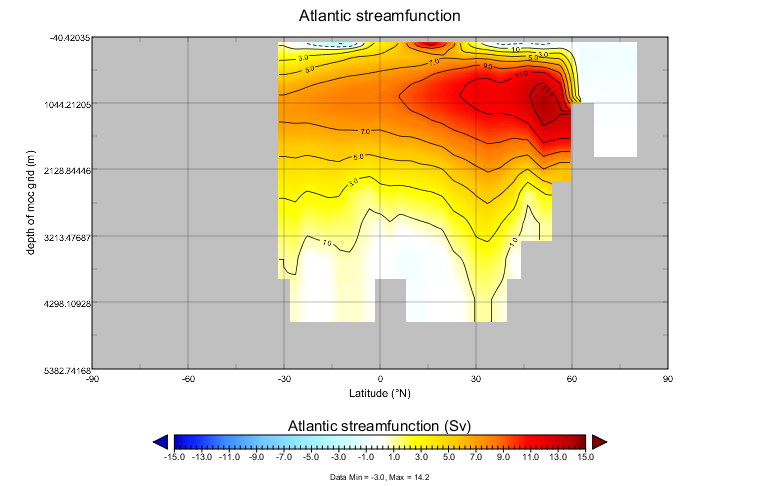
\includegraphics[width=0.6\textwidth]{ch3-amoc1.png}\centering
\vspace{-0mm}
\caption{Example plot of (normal/default modern) overturning streamfunction (2D \textbf{netCDF} file). (e.g., for Atlantic: \textbf{netCDF} parameter name: \texttt{phys\_opsia}, long-name: Atlantic streamfunction). Note that autoscaling has been turned off and the min and max plotting limits set manually. By convention, streamfunctions are plotted with their scale symmetrical around zero, giving red and ‘warm’ colors for positive value and clockwise overturning, and blues and ‘cold’ colors for negative values and anti-clockwise overturning. (The plot has been tart-ed up by overlaying solid contours plus contour labels.) It may be necessary in \textbf{Panoply} to re-orient (invert) the vertical grid.}
\label{fig:ch3-amoc1}
\end{figure}

\begin{figure}
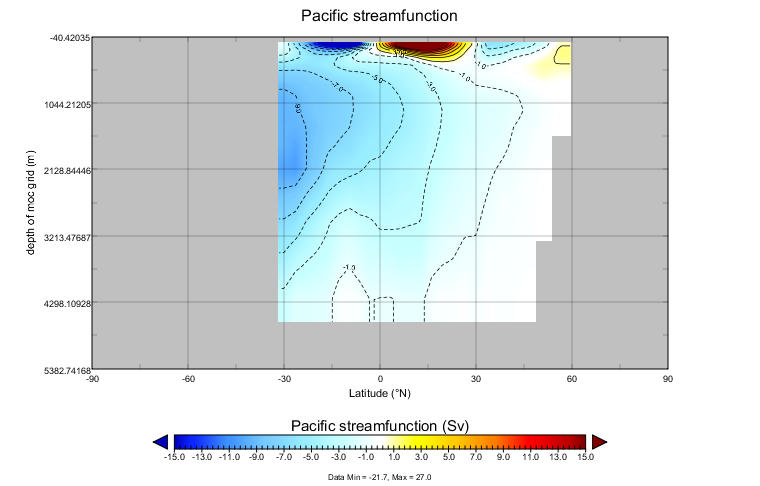
\includegraphics[width=0.6\textwidth]{ch3-amoc2.png}\centering
\vspace{-0mm}
\caption{Example plot of collapsed AMOC.}
\label{fig:ch3-amoc2}
\end{figure}

\vspace{1mm}
\noindent\rule{4cm}{0.5pt}
\vspace{2mm}

\noindent You can also plot ocean current fields which is sort-of fun and maybe even informative(!):

\vspace{1mm}
\begin{enumerate}[noitemsep]
\vspace{1mm}
\item  In the 3D \textbf{netCDF} file, the three components of ocean velocity are represented by the variables: ocean velocity – u (Eastwards), ocean velocity – v (Northwards), and ocean velocity – w (upwards). 2. Open up velocity – u. Chose ‘lon-lat’.
\vspace{1mm}
\item Select/highlight velocity – v. and click on the ‘Combine Plot’ icon (as per before).
\vspace{1mm}
\item Rather than a difference map, which is what you get by default, i.e., ‘Array 1 – Array 2’ – from the drop-down menu (next to the ‘Interpolate’ button) select ‘Vector Magnitude’.
\vspace{1mm}
\item You should have a color contoured (or not if you prefer plotting without contouring on) map of ocean current speed, with velocity vectors (direction and magnitude) overlain. You’ll need to re-scale the velocity vectors to properly see them – from the ‘Contours and Vectors’ tab – change the ‘Scale Length’ to e.g., 0.1. (On a \textbf{Mac}, look under the ‘Vectors’ tab for a ‘Reference Value’ to something like 0.1.)  When fresh-water hosing – look out for impacts on the N. Atlantic current system associated with the AMOC.
\vspace{1mm}
\item You can repeat this for deeper depth levels in the ocean – e.g., between about 1500 and 2000 m is a good place to go looking for the Western boundary current (and AMOC return) in the model (such as it exists at this low resolution) but you’ll need to re-scale the velocity vectors again (e.g., to 0.01 to less).
\end{enumerate}
\vspace{1mm}

\noindent An example plot (using \textbf{Panoply} for visualizing surface ocean current fields) is given in Figure \ref{fig:ch3-currents1}.

\begin{figure}
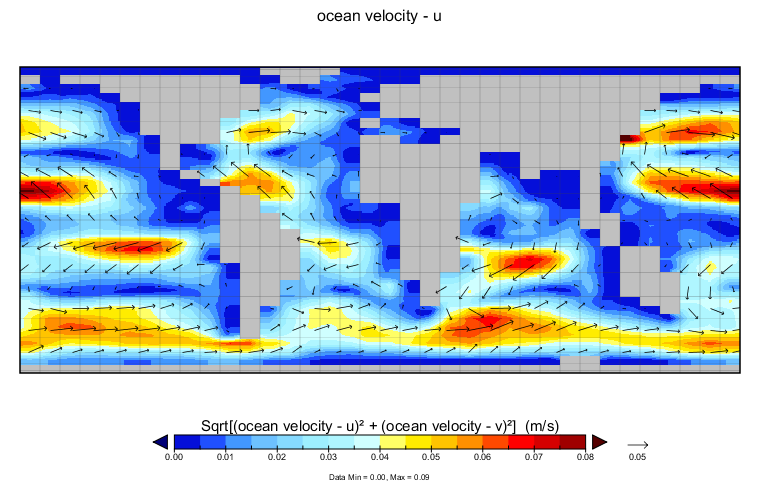
\includegraphics[width=0.6\textwidth]{ch3-currents1.png}\centering
\vspace{-0mm}
\caption{Example plot of (normal/default modern) ocean current fields (3D netCDF file). Again scaling has been set manually to create an easy-to-interpret axis scale. On the left is the surface field, and on the right an intermediate depth (illustrating what approximates the Deep Western Boundary current in the model in the Atlantic).}
\label{fig:ch3-currents1}
\end{figure}
\vspace{1mm}
\noindent\rule{4cm}{0.5pt}
\vspace{2mm}

\noindent Finally, a brief note on units ... the freshwater forcing is implemented as negative salinity, just to really screw with your mind. The generic internal \textbf{muffin} model units for the forcing end up as \(PSU kg^{-1} yr^{-1}\). Which sort of does not make much sense ...

Start, by thinking of a value of \texttt{bg\_par\_ocn\_force\_scale\_val\_2} of \(-34.9\) as equivalent to taking all the salt out of \(1 kg\) of freshwater (since the mean global salinity is \(34.9 PSU\)). Or equivalently, since the ocean volume is fixed, an applied forcing value of \(-34.9\) is equivalent to adding \(1 kg\) of freshwater to a (surface) box. So, a value of \texttt{bg\_par\_ocn\_force\_scale\_val\_2} of \(-3.49\times10^{4}\) (\(-3.49E04)\) would be a flux of \(1 m^{3} yr^{-1}\) (\(1000 kg m^{-3}\)) of freshwater.

So, in the example earlier (\texttt{bg\_par\_ocn\_force\_scale\_val\_2=-1.0E18}), the freshwater flux is \(1.0\times10^{18}/3.49\times10^{4} = 2.8653\times10^{13} m^{3} yr^{-1}\).

The literature invariably gives freshwater fluxes in units of \(Sv\) (\(10^{6} m^{3} s^{-1}\)). So in the example, the freshwater flux is: \(9.0797\times10^{5} m^{3} s^{-1}\) (\(365.25\times24\times3600 = 31557600 s yr^{-1}\)). Or \(0.9 Sv\). Read the literature … but generally, fluxes of ca. \(0.05 Sv\) and larger (and to quite specific places) are applied in models to induce an AMOC collapse.

%------------------------------------------------

\newpage

%------------------------------------------------

\section{Further ideas}

%------------------------------------------------

\subsection{Hosing investigations}

What is the largest freshwater flux that can be sustained without ‘collapsing’ the AMOC? Is there a ‘threshold’ (‘tipping point’) of freshwater input, beyond which the AMOC rapidly decreases in strength? For this -- you would run (submit to the cluster) a series of experiments, each with different (increasing) values for the fresh water flux. Remember to include an experiment with zero freshwater flux to act as a 'control'.

Is the precise location of the freshwater input important (i.e., try tipping it in somewhere else)? For this -- you could piece-meal run an experiment, analyse the results, then choose a new location to input the freshwater, or, come up with a systematic search pattern of freshwater input patterns.  

Outside of the North Atlantic, are any other major regions of deep water formation (where are they) sensitive to freshwater perturbation and what are the consequences (could it happen in the future)?

%------------------------------------------------

\subsection{‘Anti-hosing’ investigations}

There are questions concerning past changes in the AMOC as to whether it is ‘pushed’ or ‘pulled’. i.e., if the AMOC shoals in depth and/or weakens, is it because its production has weakened, or as Antarctic Bottom water (AABW) strengthened and ‘pushed’ it out of the way (to shallower depths)?

What you might try then is to inject salt in the Southern Ocean as opposed to fresh water in the North Atlantic. All you need do is pick an appropriate grid point (this is worth thinking about carefully and maybe testing different locations) and rather than giving the parameter \texttt{bg\_par\_ocn\_force\_scale\_val\_2} a negative value, you give it a positive one. (Start by trying similar magnitudes of value as before and see what happens.)

\textbf{Is the AMOC (for the same magnitude of forcing) more sensitive to being ‘pushed’ or ‘pulled’?} (Obviously the answer will very much depend on where the perturbations are being applied.)

%------------------------------------------------

\subsection{Response to transient warming}

A current concern regarding anthropogenic climate change is the ocean circulation (and marine ecological and biogeochemical) response to a strong warming of the surface, as rapid surface warming is assumed (and demonstrated in models) to result in surface stratification of the ocean, likely restricting the nutrient supply to phytoplankton and reducing ventilation of the ocean interior with dissolved oxygen.

You can explore the transient response of ocean circulation to warming by simply adjusting the radiative forcing parameter as per used in the snowball Earth experiments: \texttt{ea\_radfor\_scl\_co2}. By default in the modern continental configuration, this has a value of 1.0, corresponding to 278 ppm atmospheric \(CO_{2}\). A value of 2.0 would reflect warming equivalent to 556 ppm \(CO_{2}\). And 3.0 more like an end-of-the-century warming. Note that you are applying the warming instantaneously by manipulating the climate system in this way and hence the changes will be more extreme than those occurring over the time-scale of this century. Also note that a cooling could be applied instead. A \textit{user-config} –- \textsf{\footnotesize LAB\_2.EXAMPLE} – is provided as a template for these experiments.

Potentially interesting properties of the Earth system to look at include sea-ice extent and AMOC strength (in the ASCII time-series files), and the overturning stream-function and sea-ice extent in the 2-D \textbf{netCDF} output.

\textbf{How much radiative forcing is required to collapse the AMOC? What atmospheric \(CO_{2}\) value does this approximately correspond to?
}

%------------------------------------------------

\subsection{Ventilation age tracers}

\textbf{muffin} has the capability to employ/simulate a ventilation age tracer\footnote{Under the '\textit{screw with and/or diagnose the climate system}' HOW-DO -- see '\textit{Add a water mass age tracer}' (and the 'easy'/automatic method described towards the end of that section).} -- a numerical tracer in the ocean that tracks the time since a parcel of water last 'saw' the surface. To do this, requires both 'red' and 'blue' numerical tracers to be selected.  \textbf{muffin} can then be directly to automatically apply the forcings necessary to each tracer in order to simulate water mass ventilation age.

Provided is an additional \textit{user-config} file: \textsf{\footnotesize muffin.worjh2.NONE\_colage.EXAMPLE}.

A new \textit{re-start} experiment is provided called \texttt{muffin.worjh2.NONE\_colage.SPIN} and which can be downloaded as per before:

\vspace{-1mm}
\small
\begin{verbatim}
$ wget http://www.seao2.info/cgenie_output/muffin.worjh2.NONE_colage.SPIN.tar.gz
\end{verbatim}
\normalsize
\vspace{-1mm}

\noindent and unpacked, as before, by:

\vspace{-1mm}
\begin{verbatim}
$ tar xfzv muffin.worjh2.NONE_colage.SPIN.tar.gz
\end{verbatim}
\vspace{-1mm}

\noindent (Remember: you should be in the \texttt{cgenie\_output} directory when you do this.)

To run (e.g. for 10 years), following on from its \textit{re-start} experiment:

\vspace{-1mm}
\small
\begin{verbatim}
$ ./runmuffin.sh cgenie.eb_go_gs_ac_bg.worjh2.rb LABS muffin.worjh2.NONE_colage.EXAMPLE
    10 muffin.worjh2.NONE_colage.SPIN
\end{verbatim}
\normalsize
\vspace{-1mm}

\noindent (all on one line)

In the 3D netCDF output file -- \textsf{\footnotesize misc\_col\_Dage} is the output variable that is the calculated ventilation age.

First -- explore the distribution of water mass age and think about the physical ocean circulations reasons for this. Are all the modelled distributions reasonable? Are there indicators of facets of the simulated circulation that are not particularly realistic? Try plotting both lon-lat and lat-depth slices through the ocean.

Secondly -- you could additionally combine this experiment configuration with fresh water hosing, or a prescribed radiative forcing (and warming), and explore how ocean ventilation responds as ocean circulation changes. (You'll need to create for yourself a new \textit{forcing} directory and set of files that now combines both color tracers AND a freshwater flux.)

%----------------------------------------------------------------------------------------
%       CHAPTER 4
%----------------------------------------------------------------------------------------

\cleardoublepage

\chapterimage{Jay-Matternes---EOCENE.jpg} % Chapter heading image

\chapter{Climates of Past Worlds}\label{ch:past-worlds}

\hfill \break

\vspace{12mm}

\noindent This Chapter comprises 2 different exercises, both employing 'realistic' reconstructions of past continental configuration and climate and designed to explore some of the key controls on global surface climate as well as the spatial pattern of surface temperatures.

The two exercises concern the late Cretaceous and early Eocene climate states, and are somewhat interchangeable.

\section*{Background reading (Cretaceous climate)}
\begin{itemize}
\item Barron, E.: A warm equable Cretaceous: the nature of the problem, Earth-Science Reviews 19, 305–338, 1983.
\item Bice, K. L., and R. D. Norris, Possible Atmospheric \(CO_{2}\) extremes of the middle Cretaceous (late Albian-Turonian), Paleoceanography 17, doi: 10.1029/2002PA000778, 2002.
\item Bice, K. L., B. T. Huber, and R. D. Norris, Extreme polar warmth during the Cretaceous greenhouse?: Paradox of the Late Turonian \(d18O\) record at DSDP Site 511, Paleoceanography 18, doi: 10.1029/2002PA000848, 2003.
\item Bice, K. L., D. Birgel, P. A. Meyers, K. A. Dahl, K. Hinrichs, and R. D. Norris, A multiple proxy and model study of Cretaceous upper ocean temperatures and atmospheric \(CO_{2}\) concentrations, Paleoceanography 21, PA2002, doi:10.1029/2005PA001203, 2006.
\item Donnadieu, Y., et al., Modelling the primary control of paleogeography on Cretaceous climate, Earth and Planetary Science Letters 248, 426–437, 2006.
\item Huber, B. T., Norris, R. D., and MacLeod, K. G.: Deep-sea paleotemperature record of extreme warmth during the Cretaceous, Geology 30, 123–126, 2002.
\item Hunter, S. J., et al., Modelling Maastrichtian climate: investigating the role of geography, atmospheric \(CO_{2}\) and vegetation, Clim. Past Discuss. 4, 981–1019, 2008.
\item Jenkyns, H. C., Forster, A., Schouten, S., and Sinninghe Damste, J. S.: High temperatures in the Late Cretaceous Arctic Ocean, Nature 432, 888–892, 2004.
\end{itemize}

\section*{Background reading (Eocene climate)}
\begin{itemize}
\item Dunkley Jones, T., D.L. Lunt, D.N. Schmidt, A. Ridgwell, A. Sluijs, P.J. Valdes, and M. Maslin, Climate model and proxy data constraints on ocean warming across the Paleocene-Eocene Thermal Maximum, Earth-Science Reviews 125 123–145 (2013).
\item Lunt, D. J., Dunkley Jones, T., Heinemann, M., Huber, M., LeGrande, A., Winguth, A., Loptson, C., Marotzke, J., Roberts, C. D., Tindall, J., Valdes, P., and Winguth, C.: A model–data comparison for a multi-model ensemble of early Eocene atmosphere–ocean simulations: EoMIP, Clim. Past, 8, 1717-1736, doi:10.5194/cp-8-1717-2012, 2012.
\end{itemize}

%------------------------------------------------

\newpage

%------------------------------------------------

\section*{READ.ME}

You will need to download new \textit{restart} files for this Chapter (both 10,000 year spin-ups). These are:

\vspace{2mm}
\begin{enumerate}[noitemsep]
\item[\textbf{Cretaceous:}]
\begin{verbatim}
$ wget http://www.seao2.info/cgenie/labs/AWI.2017/LAB_5.SPIN.tar.gz
\end{verbatim}
\item[\textbf{Eocene:}]
\begin{verbatim}
$ wget http://www.seao2.info/cgenie/labs/AWI.2017/LAB_5b.SPIN.tar.gz
\end{verbatim}
\end{enumerate}
\vspace{2mm}

Extract the results in the usual way and in the usual place ... and return to \texttt{genie-main}.

%------------------------------------------------

\newpage

%------------------------------------------------

\section{The climate of the Cretaceous}

A previously spun-up state of Maastrichtian climate with \textbf{cGENIE.muffin} in a ca. 70 Ma configuration\footnote{Note that for speed, no carbon cycle is selected in this configuration.} (\texttt{LAB\_5.SPIN}) is provided as a starting point. A \textit{user-config} (\texttt{LAB\_5.EXAMPLE}) that continues on this climate state is run:
\begin{verbatim}
$ ./runmuffin.sh cgenie.eb_go_gs_ac_bg.p0067f.NONE LABS
 LAB_5.EXAMPLE 10 LAB_5.SPIN
\end{verbatim}

Your task now is ... ‘simple’: Account for the Cretaceous reduced Equator-to-pole surface temperature gradient (compared to modern), particularly the apparently much warmer poles. Different data-based time-slices (including the Maastrichtian) are provided in \textit{Huber et al.} [2002], although the low latitude \(\delta^{18}O\) based temperatures are now not considered reliable. \textit{Jenkyns et al.} [2004] contains high latitude (Arctic) data for the Maastrichtian. There are proxy-derived latitudinal temperature gradients and model-data studies for earlier in the Cretaceous – the problem is essentially the same.

The 2-D NetCDF results file contains the surface air temperature field (and sea-ice cover, if any). The 3-D NetCDF results file contains fields for ocean temperatures (and salinity). Both contain continental configuration and ocean bathymetry.

\textbf{Panoply} will plot the zonal average for you (as used in model-data comparisons – e.g., see Bice and Norris [2002]) – in the Array(s) tab, the Plot can be set to Zonal Averages rather than Map. You can get a smooth curve by selecting Interpolate. Remember you can set (and fix) scales rather than let Panoply auto-scale continually.

The following ‘controls’ over the climate system are provided to you in the form of a list of parameters at the bottom of the \texttt{LAB\_5.EXAMPLE} \textit{user-config} file for editing:

\small\begin{verbatim}
# --- MISC -----------------------------------------------
#
# === ATMOSPHERE ===
# \(CO_{2}\) radiative forcing scaling factor [DEFAULT = 4.0]
ea_radfor_scl_co2=4.0
# CH4 radiative forcing scaling factor [DEFAULT = 1.0]
ea_radfor_scl_ch4=1.0
# Equator-to-pole different in planetary albedo [DEFAULT = 0.260]
ea_albedop_amp=0.260
# Baseline planetary albedo [DEFAULT = 0.200]
ea_albedop_offs=0.200
# atmospheric diffusivity of temperature (horizontal) [DEFAULT = 5.0e6]
ea_12=5.0e6
# === OCEAN ===
# ocean diffusivity of temperature + salinity (horizontal) [DEFAULT = 1494.4]
go_14=1494.4
# scaling for wind stress (set values of both identical) [DEFAULT = 1.531]
go_13=1.531
ea_11=1.531
\end{verbatim}\normalsize

Most of these parameters are associated with the radiative forcing of climate or atmospheric transports. The most useful ones are likely to be:

\begin{itemize}[noitemsep]

\item[\textbf{(i)}] The line:
\begin{verbatim}
ea_radfor_scl_co2=4.0
\end{verbatim}
which specifies a radiative forcing of climate by \(CO_{2}\) equivalent to \(4\) times modern \(CO_{2}\) (i.e., \(4\times278 ppm = 1112 ppm\)) as per before (e.g. snowball Earth experiments).
\\The line:
\begin{verbatim}
ea_radfor_scl_ch4=1.0
\end{verbatim}
specifies a radiative forcing of climate by \(CH_{4}\) equivalent to \(1\) times modern \(CH_{4}\) (i.e., \(1\times700 ppb\)).\footnote{But effectively, this is going to do exactly the same as changing radiative forcing due to \(CO_{2}\).}

\item[\textbf{(ii)}] cGENIE, as configured here, does not have a land surface scheme (no snow cover) nor clouds nor ice sheets, so a planetary albedo is prescribed (see Figure 4.1). This varies with latitude and is parameterized after a fully coupled GCM simulation. There is a parameter which controls how the albedo varies as a function of latitude, which can be adjusted:
\begin{verbatim}
ea_albedop_amp=0.260
\end{verbatim}
However, if you vary this, why are you doing it? (What is the physical justification for giving the poles a higher or lower albedo relative to the Equator?)
There is also a parameter that sets the baseline (minimum) albedo:
\begin{verbatim}
ea_albedop_offs=0.200
\end{verbatim}
i.e., albedo is primarily a sum of the baseline value plus the Equator-to-pole slope (times the latitude).

\item[\textbf{(iii)}] The diffusivity of heat in the atmosphere (since it is a simple 2-D atmospheric model, with no atmospheric circulation, the atmosphere is made ‘diffusive’ to help capture heat and moisture transport) is:
\begin{verbatim}
ea_12=5.0e6
\end{verbatim}
Note the maximum value the model can cope with is ca. \(1.0E7\).

\end{itemize}

\begin{figure}
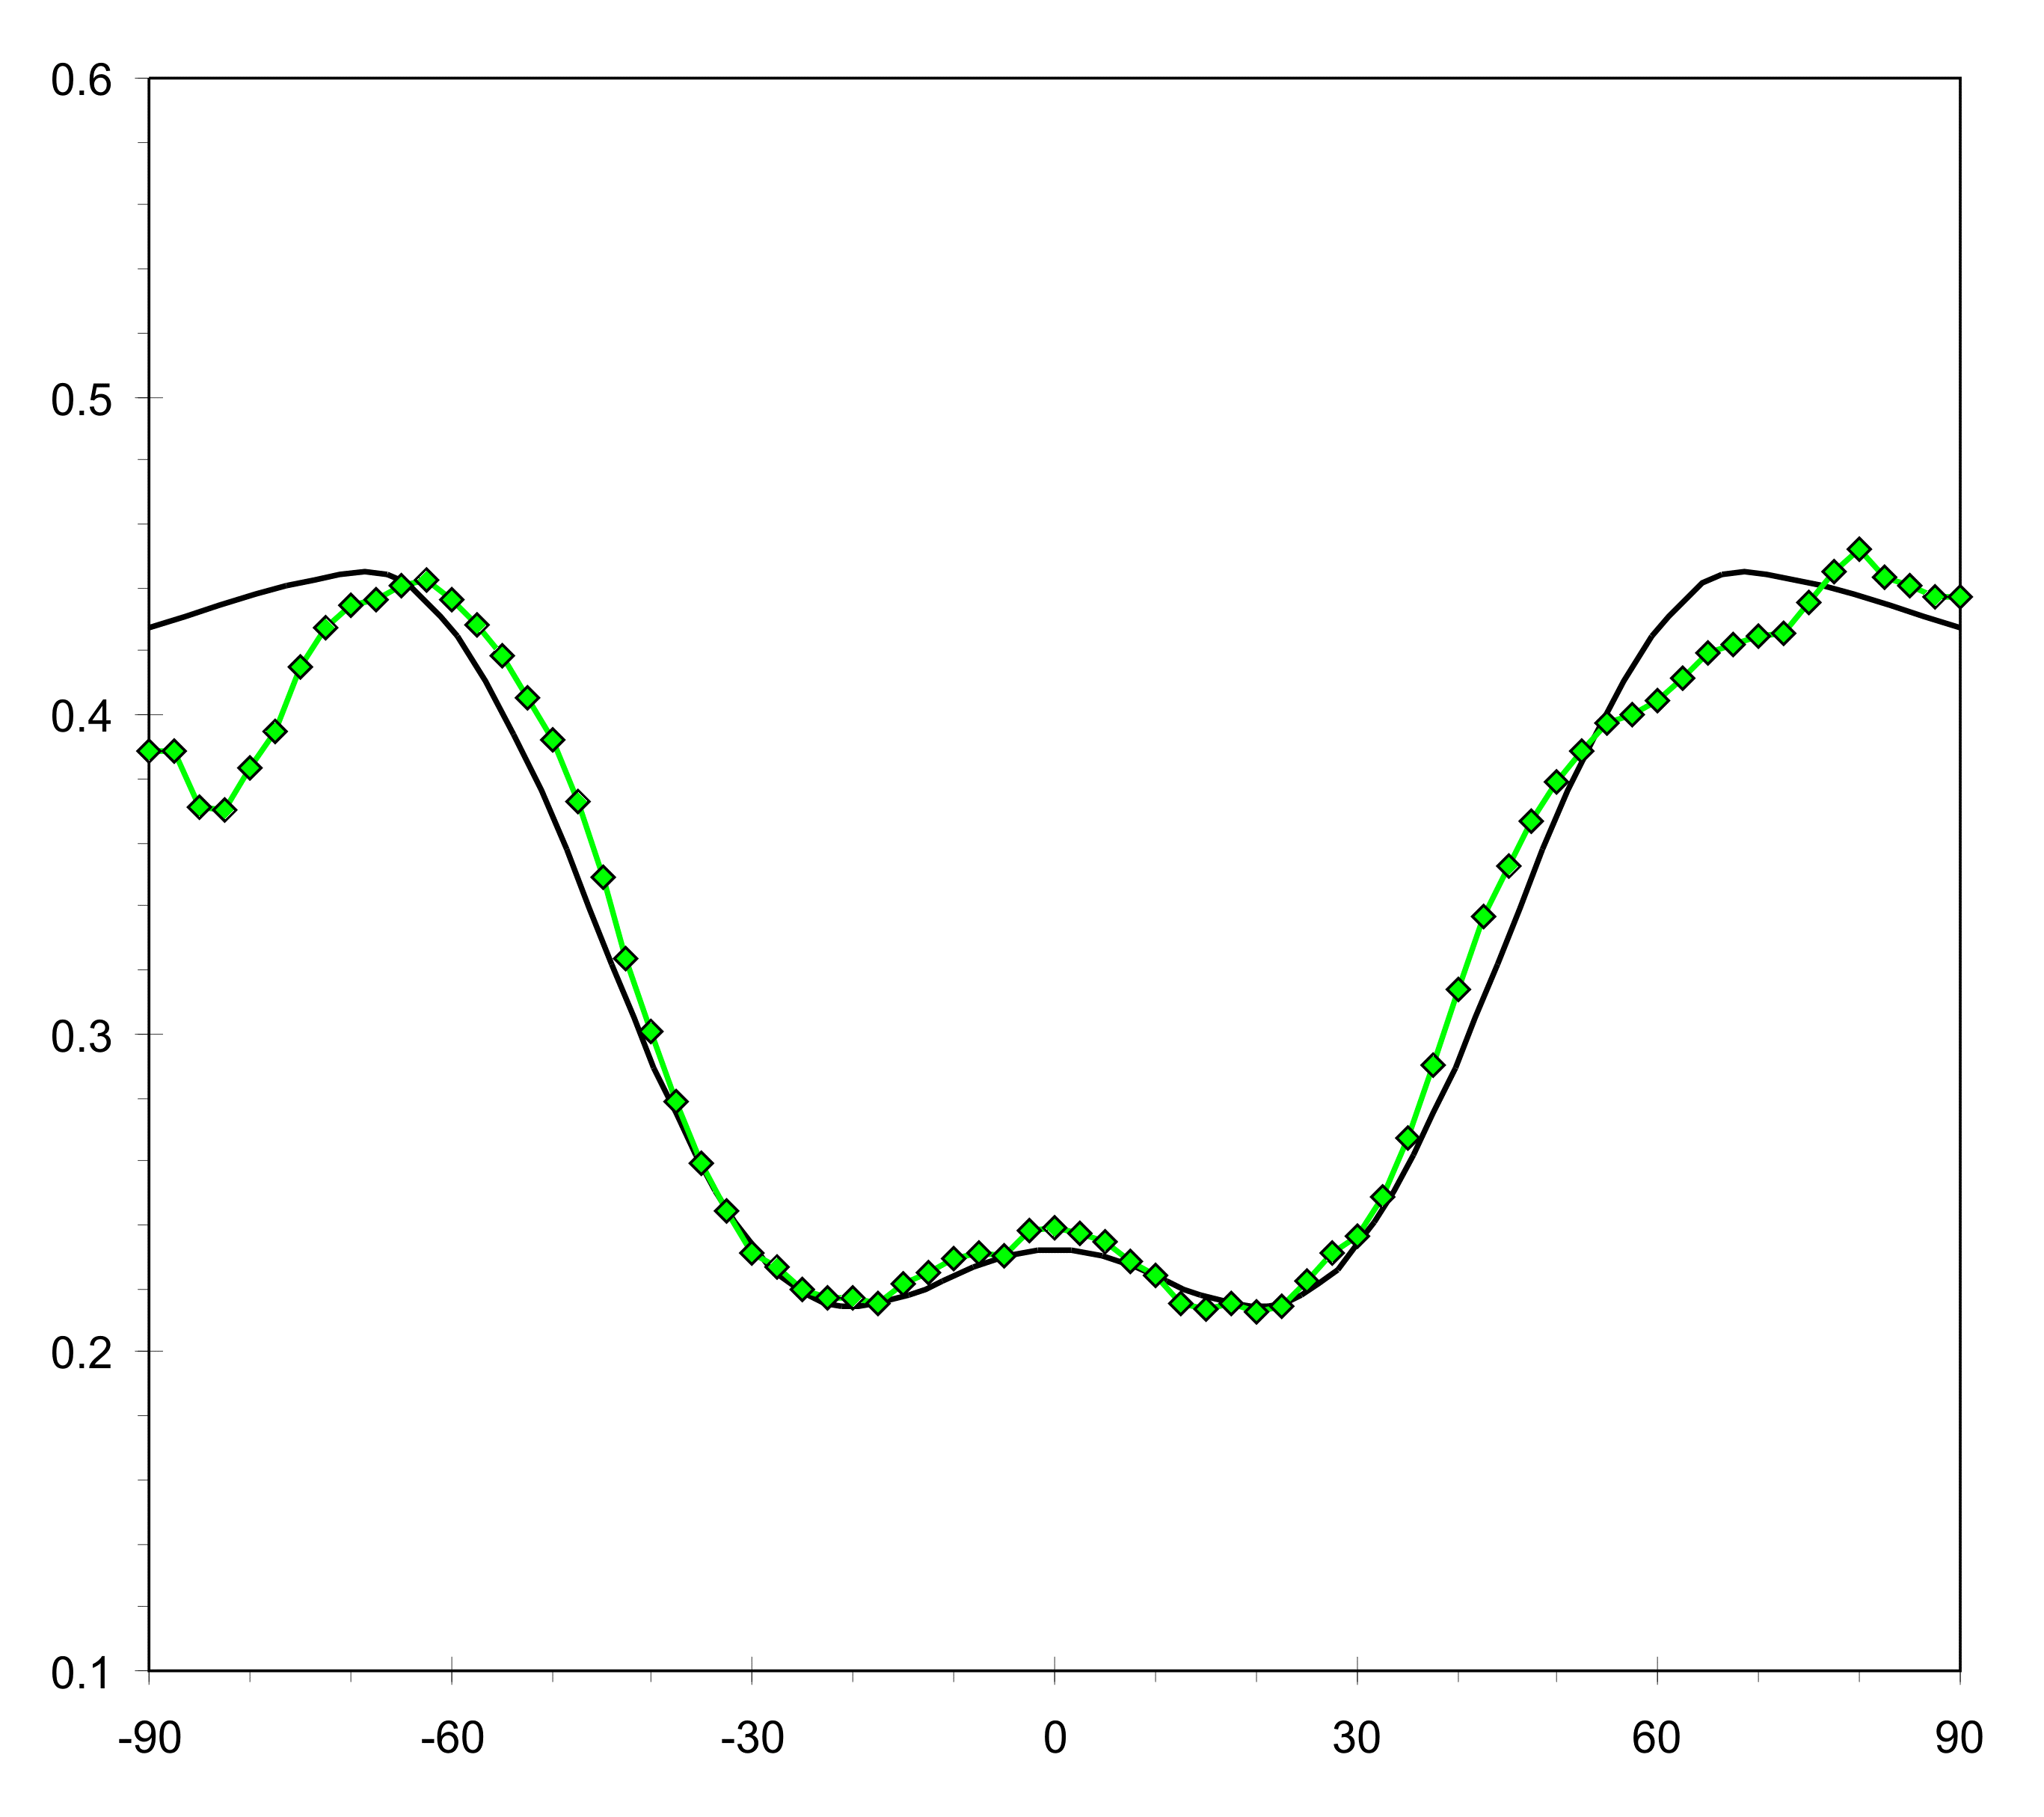
\includegraphics[width=0.6\textwidth]{tmp-albedo.png}\centering
\vspace{-6mm}
\caption{Prescribed planetary albedo.
The latitudinal (from 90$^{\circ}$S (-90$^{\circ}$N) on the left, to 90$^{\circ}$N on the right) profile of planetary albedo as calculated in a fully coupled GCM is given in green, and the cGENIE ‘fit’ in black.}
\label{fig:tmp-albedo}
\end{figure}

\vspace{1mm}
\noindent\rule{4cm}{0.1mm}
\vspace{2mm}

\noindent Run the model for however long you think is ‘necessary’ (/justified). The surface climate will approach equilibrium ‘relatively’ quickly. Deep ocean temperatures will typically take thousands of years to fully adjust ... You can assess how the model approaches equilibrium most easily from the atmospheric temperature time-series results file, and from the ocean temperature time-series results file (allowing to you to contrast surface and whole ocean temperature changes).

\vspace{1mm}
\noindent\rule{4cm}{0.1mm}
\vspace{2mm}

\noindent You can also try tracing and analyzing the patterns of ocean circulation in the Cretaceous world, in the same way as you did for the modern climate system. And in fact, it would be a useful exercise to directly compare your previous modern results vs. Cretaceous results, or even better, carry out a set of paired experiments (e.g., similar locations and fluxes of dye injection) for both modern and Cretaceous. (Note that if you do this and swap back and forth between modern and Cretaceous configurations, you cannot submit straight away to the cluster but must first briefly run the experiment at the command line in order that cGENIE is compiled into the new continental configuration.)

A new \textit{user-config} (\texttt{LAB\_5.colorinjection}) that continues on from this climate state, can be run:
\begin{verbatim}
$ ./runmuffin.sh cgenie.eb_go_gs_ac_bg.p0067f.rb LABS
 LAB_5.colorinjection 10 LAB_5.SPIN
\end{verbatim}
(Also note that the \textit{base-config} is different as it now includes the definition of 2 dye tracers.)

The default locations for the dye release are set different compared to in the modern configuration. BUT, the default location is not necessarily ideal / particularly revealing … so you’ll need to look count grid cells West-to-East (the i direction) and from South to North (the j direction) in order to determine a more suitable location for tracing circulation.

By means of dye tracing, looking at the (global only) overturning stream-function, and/or temperature and salinity (and density) profiles, see if you can identify where in the Cretaceous ocean deep water forms in the model. AND, more importantly, think about WHY does it form where it does?

Also: what about surface ocean circulation and gyres? Are these located where you would expect (e.g. based on your understanding of modern ocean circulation). Plot velocity vectors to help, and/or refer to the Barotropic streamfunction output in the 2D netCDF file.

%------------------------------------------------
%
\newpage

%------------------------------------------------

\section{The climate of the early Eocene}

A previously spun-up state of early Eocene climate with cGENIE in a ca. 56 Ma configuration (\texttt{LAB\_5b.SPIN}) is provided as a starting point. A user-config (\texttt{LAB\_5b.EXAMPLE}) that continues on this climate state is run:
\begin{verbatim}
$ ./runmuffin.sh cgenie.eb_go_gs_ac_bg.p0055c.NONE LABS
 LAB_5b.EXAMPLE 10 LAB_5b.SPIN
\end{verbatim}
(Note that once again, for speed, no carbon cycle is selected in this configuration.)
Again, as per for the late Cretaceous configuration, a configuration that includes the ocean dye (color) tracers is also provided. The corresponding user-config (\texttt{LAB\_5b.colorinjection}) that continues on this climate state can be run as follows:
\begin{verbatim}
$ ./runmuffin.sh cgenie.eb_go_gs_ac_bg.p0055c.rb LABS
 LAB_5b.colorinjection 10 LAB_5b.SPIN
\end{verbatim}

\vspace{1mm}
\noindent\rule{4cm}{0.1mm}
\vspace{2mm}

\noindent What to ‘do’ with this? Again – start by tracing and analyzing the patterns of ocean circulation in the Eocene world, as per how you did for the modern and Cretaceous system. Where does deep water form in the Eocene? Is the surface ocean circulation as expected?
Can you see any patterns emerging? At least in model world – what seems to be dictating the locations of deep water formation? Does overturning and/or surface circulation appear to significantly vary as a function of continental configuration or radiative forcing? If not, why not?

\vspace{1mm}
\noindent\rule{4cm}{0.1mm}
\vspace{2mm}

\noindent But how do you know how close, or not, the model climate is to ‘reality’?
Available from the website, on the LH side of the page under ‘got data?’ at the bottom (item (7)), are 2 netCDF files containing proxy sea surface temperature (SST) data re-gridded to the cGENIE model grid. One is for pre-PETM SSTs, and one for peak PETM SSTs. (The data are from Dunkley Jones et al. [2013].)

These netCDF files can be opened and visualized in exactly the same way in exactly the same way as per the cGENIE output files. You’ll see a few (there are not many!) data points, in a sea of grey (which stands for ‘no value’). (Note that it is best to turn data interpolation OFF.)

More useful … is that the data distribution can be combined with the model ocean temperature output field, in a difference map (see earlier for notes on creating difference maps). You can thus visualize the pattern of model-data mismatch. (Note you might want to hit ‘Fit to data’ to autoscale the plot, or simply pick and manually enter a +/- limit for the data plotting, perhaps ensuring it is symmetrical about zero such that red anomalies could represent proxy SST values higher than in the model, and blue point data being lower than in the model.)

Furthermore, in the Arrays tab, you can switch to a Zonal Average view rather than a Map view (...it is probably easier to visualize the model-data misfit in this way.)

\vspace{1mm}
\noindent\rule{4cm}{0.1mm}
\vspace{2mm}

\noindent So, starting with the pre-PETM data and given model configuration, make some assessment of how the model fits the data (or not). What might be the reason for the misfit? You might test adding, and adjusting, some of the parameter values controlling surface SST from the Cretaceous climate exercise. Can you reduce the model-data misfit?

\vspace{1mm}
\noindent\rule{4cm}{0.1mm}
\vspace{2mm}

\noindent Finally, the PETM SST data given in the 2nd netCDF file are from the peak of the PETM. The ocean is rather warmer as compared to just prior to the PETM. Your task is to determine (either using the default model configuration, or your adjusted configuration) much radiative forcing (parameter \texttt{ea\_radfor\_scl\_co2}) and hence \(CO_{2}\) is required to explain this warming?

%----------------------------------------------------------------------------------------
%       CHAPTER 4
%----------------------------------------------------------------------------------------

\cleardoublepage

\chapterimage{middle_earth.png} % Chapter heading image

\chapter{Alternative Worlds}\label{ch:alternative-worlds}

\hfill \break

\noindent Fake (alternative) Worlds are a useful tool for developing a general understanding of how climate (and ocean circulation) and global biogeochemical cycles operate. Different model resolutions and continental configurations can be generate and run to test specific hypotheses about the role and sensitivity of different elements in Earth system to emergent patterns of climate (and biogeochemical cycling). Ensembles of differing Worlds can also be utilized to more generalize understanding as well as in a fishing expedition of new or unexpected phenomena and system behaviours.

This Chapter will take you through the generation and exploration (analysis) of fake (alternative) Worlds.

%------------------------------------------------

\newpage

%------------------------------------------------
%
\section{Generating fake Worlds}

%------------------------------------------------

\vspace{1mm}
\noindent\rule{4cm}{0.5pt}
\vspace{2mm}

\noindent\textcolor{red}{TO COME ...}

\vspace{1mm}
\noindent\rule{4cm}{0.5pt}
\vspace{2mm}

%------------------------------------------------

\newpage

%------------------------------------------------
%
\section{Understanding ocean circulation}

%------------------------------------------------

What follows, outlines different ways of visualizing and quantifying ocean circulation in \textbf{muffin}, and coming to a model-empirical understanding of ocean circulation controls.

%------------------------------------------------

\subsection{Model investigation over-view}

In restricting model-based experiments and derived understanding to   the modern continental configuration (and climate) in \textbf{muffin}, you'd be unlikely to come to any particularly deep or fundamental insights into ocean circulation controls in general. In any case, the modern and future (and recent glacial past) ocean circulation states and dynamics has been picked at endlessly by 1000s of researchers, writing 100,000s of  publications ... and yet still we do not fully understand modern ocean circulation, let along that at the last glacial.

A better (more fun) approach is to generalise the problem and consider fundamentally different configurations of ocean basins and climate. This is what you will be doing. But first, some potted advice:

\vspace{2mm}
\begin{itemize}[noitemsep]
\vspace{1mm}
\item Try and define a hypothesis, or hypotheses, to pursue and test. These need only be very rough at the outset -- you'll likely find that you get new ideas and can either refine your original hypotheses, or come up with new ones, as you start to play with the model and see what is feasible and not feasible in terms of analysis.
\vspace{1mm}
\item Create a plan of study -- what sort of experiments, now many, how are they going to be analysed, how do they all fit together in addressing the overarching hypotheses? Again -- it is very likely that your plan will evolve, but try and start out with something to guide you rather than wandering randomly in model world ...
\vspace{1mm}
\item For creating and an using different worlds -- create a list or table of the configurations to be explored, and summarize what you are finding. It might be helpful to plan out on paper first, some of the main continental configurations you need to create and then test in the model. (Again, this will evolve.)
\vspace{1mm}
\item Once you have some sort of idea what are are going to do -- plan the work. This is important because to run the model to steady state is not trivial. Perhaps plan on having to run the model for 5,000 years\footnote{Even so, you should try running the model much longer to be confident that 5,000 years is OK (and sufficiently close to final equilibrium).} in order to achieve a fully spun up ocean circulation state. You might get away with shorter runs, but know in advance what sort of error this would induce and is it 'important'? Once you have a list and know how long each might take, you can plan out when they will be run on the cluster (presumably on the queue) and when the results will be analysed. Note that it is a virtual certainty that once you have analysed the results of the first set of experiments, you will want something different (and will then need to revise the plana and list of experiments and analysis etc.).
\end{itemize}
\vspace{2mm}

\noindent Overall -- scientific investigations with simplified (and relatively fast) Earth system models tends to become a somewhat iterative undertaking and can involve significant trail-and-error. (This is healthy and to be expected and even enjoyed!) Rarely, can you devise at the outset, a single run or set of experiments, and it turns out this is completely sufficient. If you do not see something you do not understand in the results of the initial model experiments, you are either God (e.g. the Spaghetti Monster or Invisible Pink Unicorn), or not doing it properly. Expect to see things that interest you and lead you off on a tangent (hopefully -- this is how research should be).

Finally -- \uline{note} that in swapping between different continental configurations, \textbf{muffin} currently requires the model executable to be  re-compiled.\footnote{Note that if the \textit{base-config} is the same as the previous experiment, but you have changed a parameter value (in the \textit{user-config}), you do not need to re-compile.} This ... cannot happen on the compute nodes of the cluster if you submit an experiment using a different \textit{base-config}. When changing to a new \textit{base-config}: \uline{first}, run the model briefly interactively (i.e. at the command line). Once it has compiled (and started running), the experiment can be killed (\textsf{ctrl-c}) and now it is good to submit to the queue as a job. In any case, in utilizing a new configuration that you may never have used before, it is good practice to test it first (e.g. watch it run for a short period).

%------------------------------------------------

\subsection{Deep-water formation (\& baroclinic circulation)}

The first investigation is to investigate the controls on the strength and large-scale structure of ocean circulation, particularly in terms of the global meridional overturning circulation (MOC), and associated with this -- the primary sites of deep-water formation.

There are presumably 2 key controls to this:

\vspace{2mm}
\begin{enumerate}
\item \textbf{Temperature.}
\\This is presumably mostly a function of latitude (i.e. the further North or South, the more suitable the site will tend to be for deep-water formation) and to some extent season. There will also be an influence of the prescribed planetary albedo (which includes the effect of clouds) as well as of sea-ice (if it exists).
\vspace{2mm}
\item \textbf{Salinity.}
\\This will generally be controlled by P-minus-E -- the balance between precipitation to the ocean surface as well as fresh-water run-off form the continents, vs. evaporation from the ocean surface. Sea-ice may also be a key factor, in e.g. leading to the (seasonal) rejection of dense salty brine (and removal of freshwater to the forming ice).
\end{enumerate}
\vspace{2mm}

In turn, this suggests two sets of 'knobs' in the model that influence the patterns and magnitude of temperature and salinity across the ocean surface:

\vspace{1mm}
\begin{enumerate}
\vspace{1mm}
\item \textbf{Continental Configuration.}
\\The configuration of the continents and ocean basins will dictate the shape and location of the highest latitude ocean regions -- presumably the locations where on average, deep-water formation will occur (and hence forming the downwards/sinking limb of the MOC).
\\The relevant model 'knob' is hence how the position and orientation of continental blocks is configured on the surface of the Earth. This (creating or changing the continental configuration used by \textbf{muffin}) can all done using the \textbf{MATLAB} \textbf{muffingen} program.
\vspace{1mm}
\item \textbf{Global Climate.}
\\The mean and climate as well as the zonal temperature gradients, together with whether or not sea-ice forms (and how much), will modulate both temperature and salinity patterns at the ocean surface.
\\The model knobs here are primarily:
\begin{enumerate}
\item Atmospheric \(pCO_{2}\), or in the absence of an explicit carbon cycle, a prescribed radiative forcing:
\vspace{-2pt}\begin{verbatim}
ea_radfor_scl_co2=1.0
\end{verbatim}\vspace{-2pt}
which here, specifies \(\times1\) \(CO_{2}\) equivalent radiative forcing.
\item One could also adjust the value of the solar constant (here, given with its modern/present-day default value):
\vspace{-2pt}\begin{verbatim}
ma_genie_solar_constant=1368.0
\end{verbatim}\vspace{-2pt}
which has a subtly different effect form changing \(CO_{2}\) radiative forcing, as radiative forcing has a relatively spatially uniform impact, whereas changing the solar constant has a disproportionate impact towards the Equator (where the incident solar shortwave radiation is the greatest). So changing the solar constant is likely to impact the pole-to-Equator temperature gradient. e.g. see: Lunt, D. J., A. Ridgwell, P. J. Valdes, and A. Seale, Sunshade World.: a fully coupled GCM evaluation of the climatic impacts of geoengineering, GRL 35, L12710, doi:10.1029/2008GL033674 (2008).
\item One could also adjust the planetary albedo, particularly in respect of looking to modify the pole-to-Equator temperature. In the \textbf{muffingen} created configurations, there is an explicit 1D file specifying the zonal (with latitude) planetary albedo profile:
\vspace{-2pt}\begin{verbatim}
xxxxxxxx.albd.dat
\end{verbatim}\vspace{-2pt}
where \texttt{xxxxxxxx} is the 8-character name of the \textbf{muffingen} created World. It would be a simple matter of editing the values in the file (between the range of 0.0 and 1.0, for  perfectly absorbing, and perfectly reflective, respectively).\footnote{Best to make a copy of the original file before you modify it.} Note that the file data order is North-to-South (going from top to bottom in the file).
\end{enumerate}
\end{enumerate}
\vspace{2mm}

%------------------------------------------------

\subsection{Gateways and barotropic flow}

The overarching question in the context of ocean gateways and barotropic flow, is a little harder to define succinctly; it has to do with the details of the degree of alignment (or not) of the prevailing wind (stress)
with  gateways, and the degree to which this give rise to strong zonal ocean flow. A good and obvious modern example is the existence of the Drake Passage, between the northern tip of the Antarctic Peninsular, and the southern tip of Souther America, how this aligns with the prevailing Westerlies in the Southern Hemisphere, and hence the nature and strength of the ACC (Antarctic Circumpolar Current).

So the question naturally arises: how misaligned does a gateway have to be relative to the prevailing wind stress maximum, before the circumpolar (or circum-equatorial) flow ceases. What about having multiple gateways and their relative alignment, including what happens if one gateway is aligned with Westerly wind stress, and a second with Easterly wind stress -- who 'wins')? Also -- what about sill depths? For the Drake Passage, the ocean floor, while tectonically messy, is generally relatively deep. What happens to ocean circulation with a progressively shallow sill depth?

The 3 key controls in this exercise are then:

\vspace{2mm}
\begin{enumerate}
\vspace{1mm}
\item \textbf{Gateway alignment.}
\\The degree of alignment (or latitudinal correspondence) of a gateway with the maximum of the zonal wind stress. (For multiple gateways, what if one aligns with a wind-stress maximum of the opposite sign?)
\vspace{1mm}
\item \textbf{Gateway width.}
\\The width of a gateway (and how important this is in exerting control on ocean circulation).
\vspace{1mm}
\item \textbf{Sill depth.}
\\The sill depth! This could be uniform in depth across the gateway (easiest/best) or could be varying (probably not so easy to learn anything).
\end{enumerate}
\vspace{2mm}

The importance of the position of the gateways is primarily only in the context of the position of the maxima in the wind-stress field. In theory, the shape of the assumed zonal wind-stress could be altered ... but the wind stress needs to be defined on 2 different ocean grids  ... and this gets messy ...

As before, there are a number of changes that can be made in the model to explore the consequences of varying gateway position and sill depth (and knobs, turned):

\vspace{2mm}
\begin{enumerate}
\vspace{1mm}
\item \textbf{Land-sea mask.}
\\The model knob is hence how the width and location of gateways has bene defined in the land-sea mask. There is also the question of how many gateways (and their respective position).
\\As before, this (creating or changing the continental configuration used by \textbf{muffin}) is all done using the \textbf{MATLAB} \textbf{muffingen} program. Any of the given example \textbf{muffingen} configurations: \textsf{drakeworld}, \textsf{eqpasworld}, \textsf{ridgeworld}, or \textsf{waterworld}, could be taken as starting points -- copying and renaming the configuration \textsf{.m} file, as well as the \textsf{.dat} file in the \textsf{INPUT} directory.
Or start from scratch and a the 'blank' (initially all ocean) example configuration.\vspace{1mm}
\item \textbf{Ocean bathymetry.}
\\The bathymetry (ocean floor depth) can be changed to alter the sill depth. The easiest way to do this is probably within the \textbf{muffingen} editor, ensuring the following input parameter setting is set:
\vspace{-2pt}\begin{verbatim}
opt_user=true; % [false/true] enable user input to grid
\end{verbatim}\vspace{-2pt}
in the configuration \textsf{.m} file. (One might also then 'draw' in the gateways by hand at the same time.)
\\Note that a gap between 2 land masses must be \uline{2 or more cells wide}, to count as a gateway and allow barotropic flow in \textbf{muffingen}).
\vspace{1mm}
\item \textbf{Wind stress strength.}
\\Although it is messy to attempt to edit the profile of the applied wind-stress field, it is possible to scale its impact on ocean circulation lower and higher. The \textbf{muffin} parameter for this is:
\vspace{-2pt}\begin{verbatim}
go_13=1.531013488769531300
ea_11=1.531013488769531300
\end{verbatim}\vspace{-2pt}
Somewhat bizarrely ... it appears twice ... with different parameter names. Both parameters must be changed to the same value. Place these lines (of the new parameter value assignments) in the \textit{user-config} file for the experiment. Higher values result in a stronger applied wind-stress on the ocean surface.
\\Note that although this is the simplest change to make, it may not have such a clear scientific question associated with it (other than the obvious and trivial).
\end{enumerate}
\vspace{2mm}

%------------------------------------------------

\subsection{Analysis}

How do you 'judge' the strength and characteristics of deep-water formation, global overturning, and circulation patterns and strength, in general, or their climate (or biogeochemical) impacts? This is not a trivial question. Often, additional ocean tracers are employed in models to generate a quantitative measure of the age of a parcel of water (mean time since it last saw the surface), of some measure of the efficiency of ventilation, or large-scale transport at the surface or at depth.\footnote{We'll see such tracers employed later in the course.} Or rather involved analysis of ocean physics and transport might be employed.

One starting point is to read some of the literature where the climate properties of various hypothetical worlds have been investigated. Such as:

\begin{itemize}[noitemsep]
\item \textit{Marshall et al.} [2007] -- 'Mean Climate and Variability of the Atmosphere and Ocean on an Aquaplanet', \textit{Journal of the Atmospheric Sciences} \textbf{64}.
\item \textit{Enderton and Marshall} [2009] -- 'Explorations of Atmosphere--Ocean--Ice Climates on an Aquaplanet and Their Meridional Energy Transports', \textit{Journal of the Atmospheric Sciences}.
\item \textit{Ferreira et al.} [2010] -- 'Localization of Deep Water Formation: Role of Atmospheric Moisture Transport and Geometrical Constraints on Ocean Circulation', \textit{Journal of Climate} \textbf{23}.
\item \textit{Smith et al.} [2006] -- 'Global Climate and Ocean Circulation on an Aquaplanet Ocean–Atmosphere General Circulation Model',  \textit{Journal of Climate} \textbf{19}.
\end{itemize}

In addition, the sub-sub-sections that follow outline some simple diagnostics and ways of going about some quantitative analysis.

%------------------------------------------------

\subsubsection{Simple/global diagnostics}

\vspace{1pt}
\begin{itemize}[noitemsep]
\vspace{1mm}
\item In the biogem output results folder, there is a time-series file named:
\vspace{-2pt}\begin{verbatim}
biogem_series_misc_opsi.res
\end{verbatim}\vspace{-2pt}
This contains a summary of the evolution with time, of the minimum and maximum (anywhere) global overturning stream-function values.
\vspace{1mm}
\item Another simple property of the climate system that you might consider, is the pole-to-equator temperature gradient, both in terms of atmospheric temperature, and ocean surface temperature\footnote{\textbf{Panoply} has an option for plotting the zonal mean, from which you could read off pole-to-equator temperature gradients.} (although they should presumably be closely coupled).
\\Why? Because the large scale (overturning) circulation of the ocean should be transporting heat from the high latitude surface to the deep ocean. This presumably would act to reduce latitudinal temperature gradients. In contrast, a strong zonal slow might prevent latitudinal transport of heat.
\end{itemize}

%------------------------------------------------

\subsubsection{Using Panoply}

In a physics-only (T + S tracer) configuration of \textbf{muffin} you are  somewhat limited in what you can look at. A good staring point is the previous tutorial on ocean circulation and AMOC stability (in the context of the modern world, climate and continental configuration). For instance, you know already how to plot and visualize the MOC using \textbf{Panoply}. The Atlantic basin and hence the existence of an AMOC, is pretty specific and unique to the modern world, so likely you'll need to focus on the global MOC. (A good starting point is to familiarise yourself with the pattern and intensity of the modern.)

For example -- the \small\textsf{drakeworld }\normalsize configuration gives rise to a global MOC pattern as shown in Figure \ref{fig:paleo_drakeworld.opsi}.

\begin{figure}
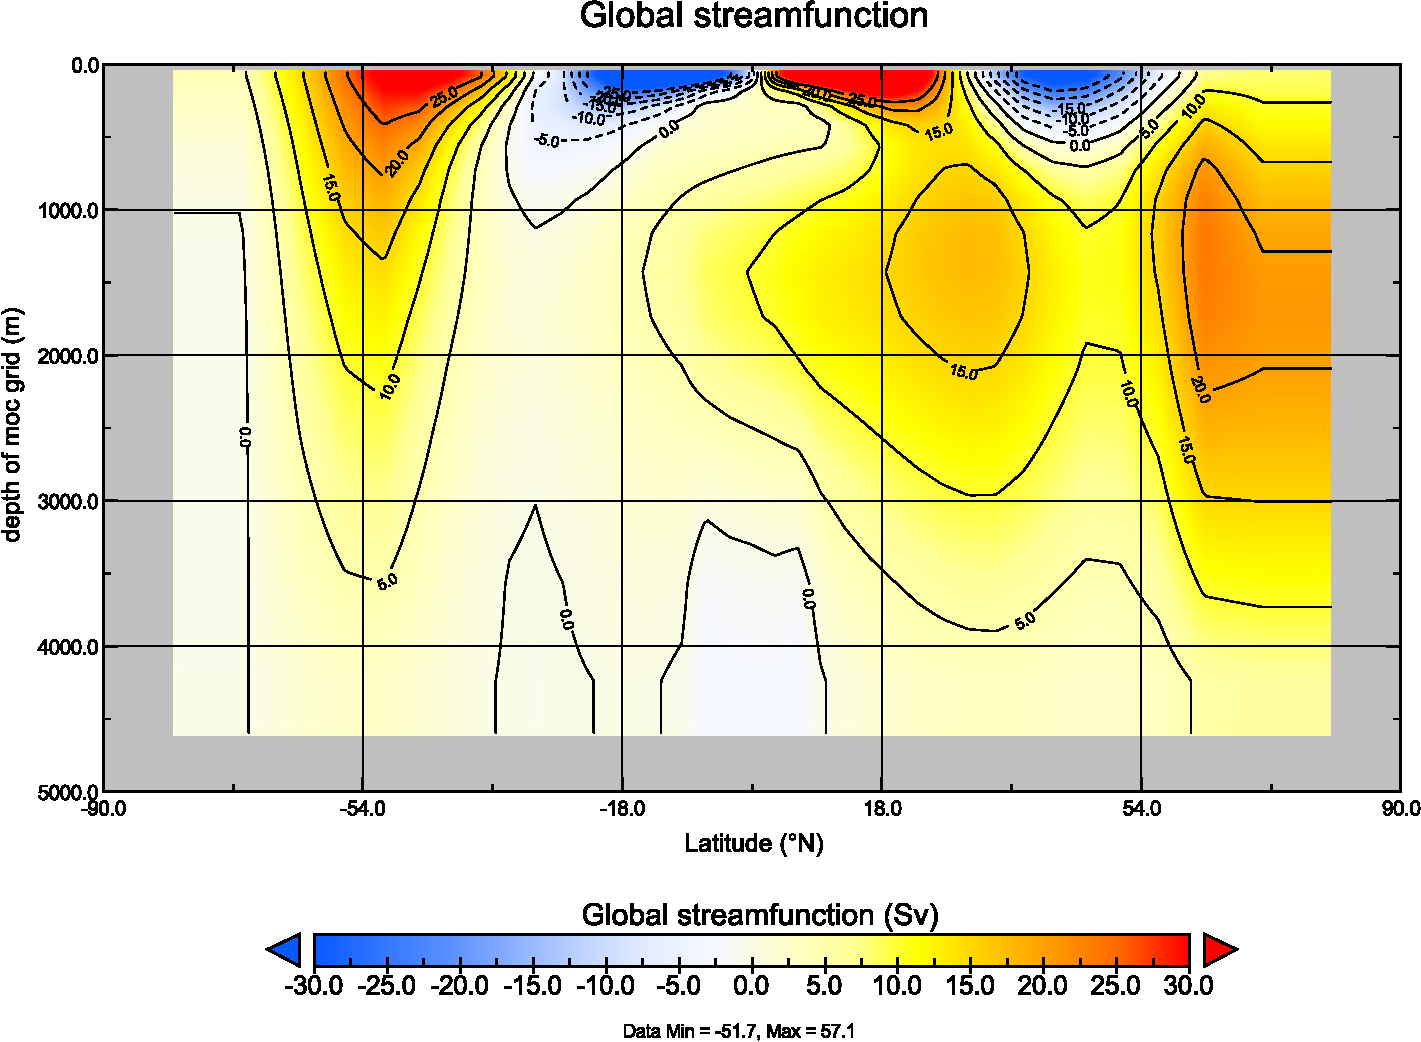
\includegraphics[width=0.6\textwidth]{paleo_drakeworld_opsi.pdf}\centering
\vspace{-6mm}
\caption{Drakework world overturning circulation.}
\label{fig:paleo_drakeworld.opsi}
\end{figure}

This is stored as the variable \small\textsf{phys\_opsi }\normalsize in the netCDF file \small\textsf{fields\_biogem\_2d.nc }\normalsize. Remember that the first time-slice plotted in \textbf{Panoply} is the first time-slice saved and it may also be up-site-down(!) by default :(.

You can also plot the barotropic circulation using \textbf{Panoply} -- the variable is called \small\textsf{phys\_psi }\normalsize -- this is shown in Figure \ref{fig:paleo_drakeworld.psi}.

Finally in \textbf{Panoply}, you might plot the current field (surface or otherwise), as per Figure \ref{fig:paleo_drakeworld.v}.

\begin{figure}
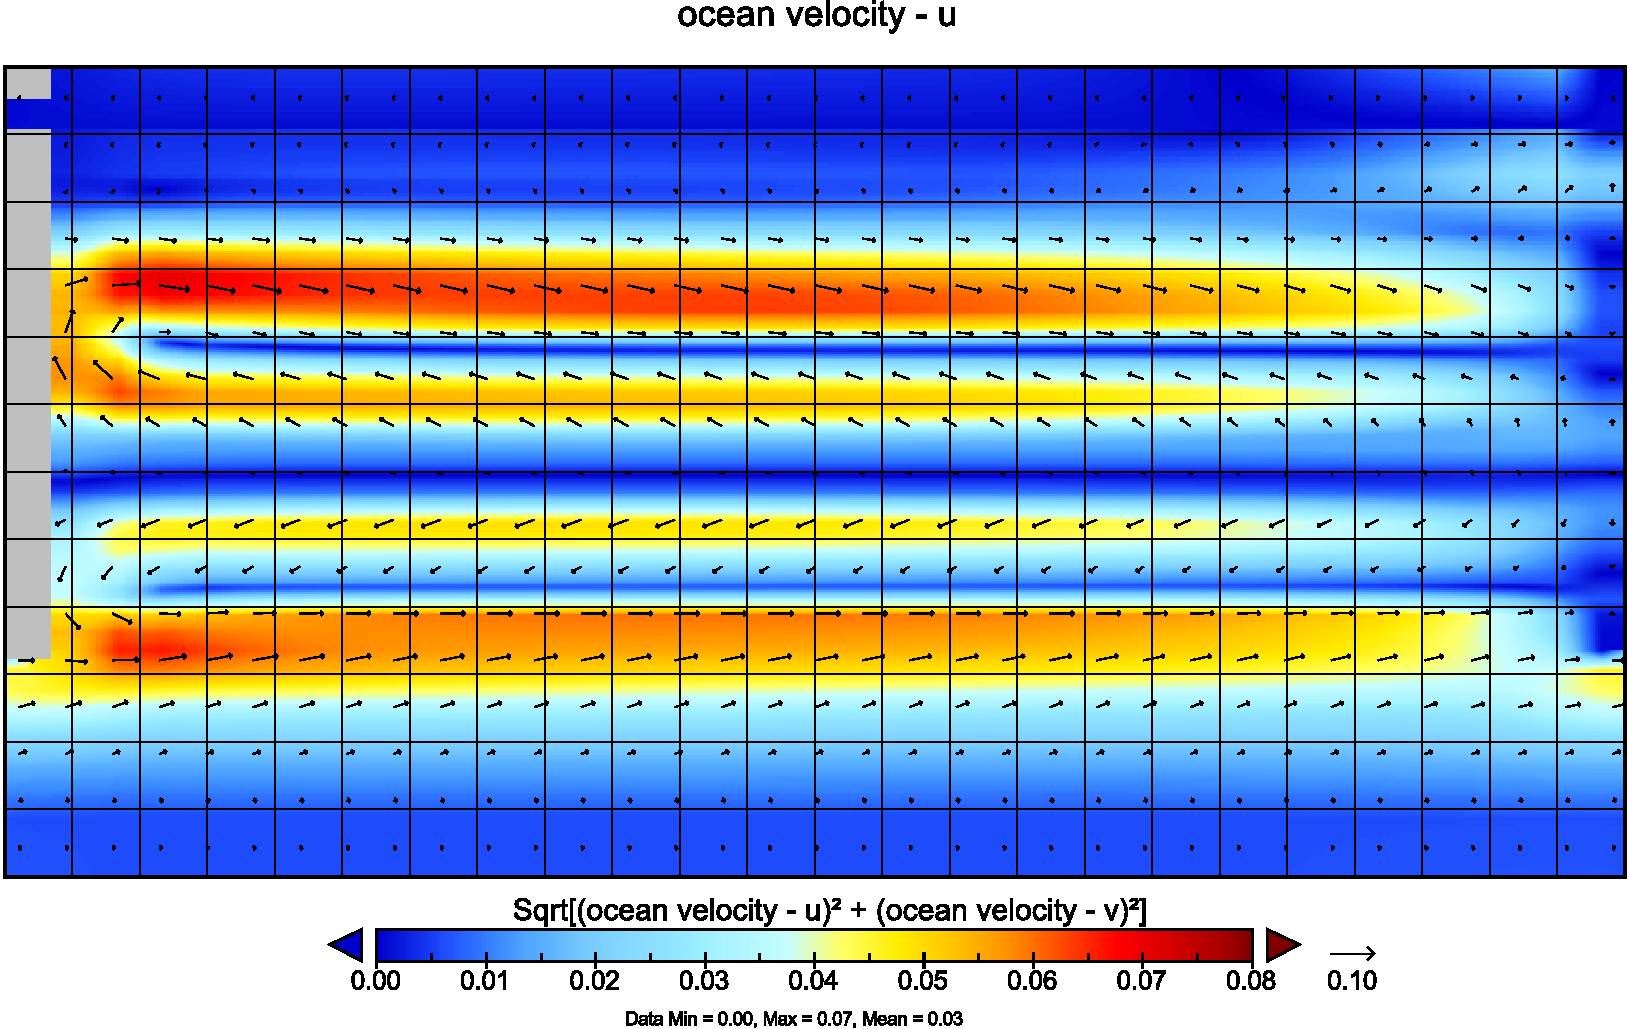
\includegraphics[width=0.5\textwidth]{paleo_drakeworld_v.pdf}\centering
\vspace{-6mm}
\caption{Surface current velocity field (arrows) plus speed (color scale).}
\label{fig:paleo_drakeworld.v}
\end{figure}

\begin{figure}
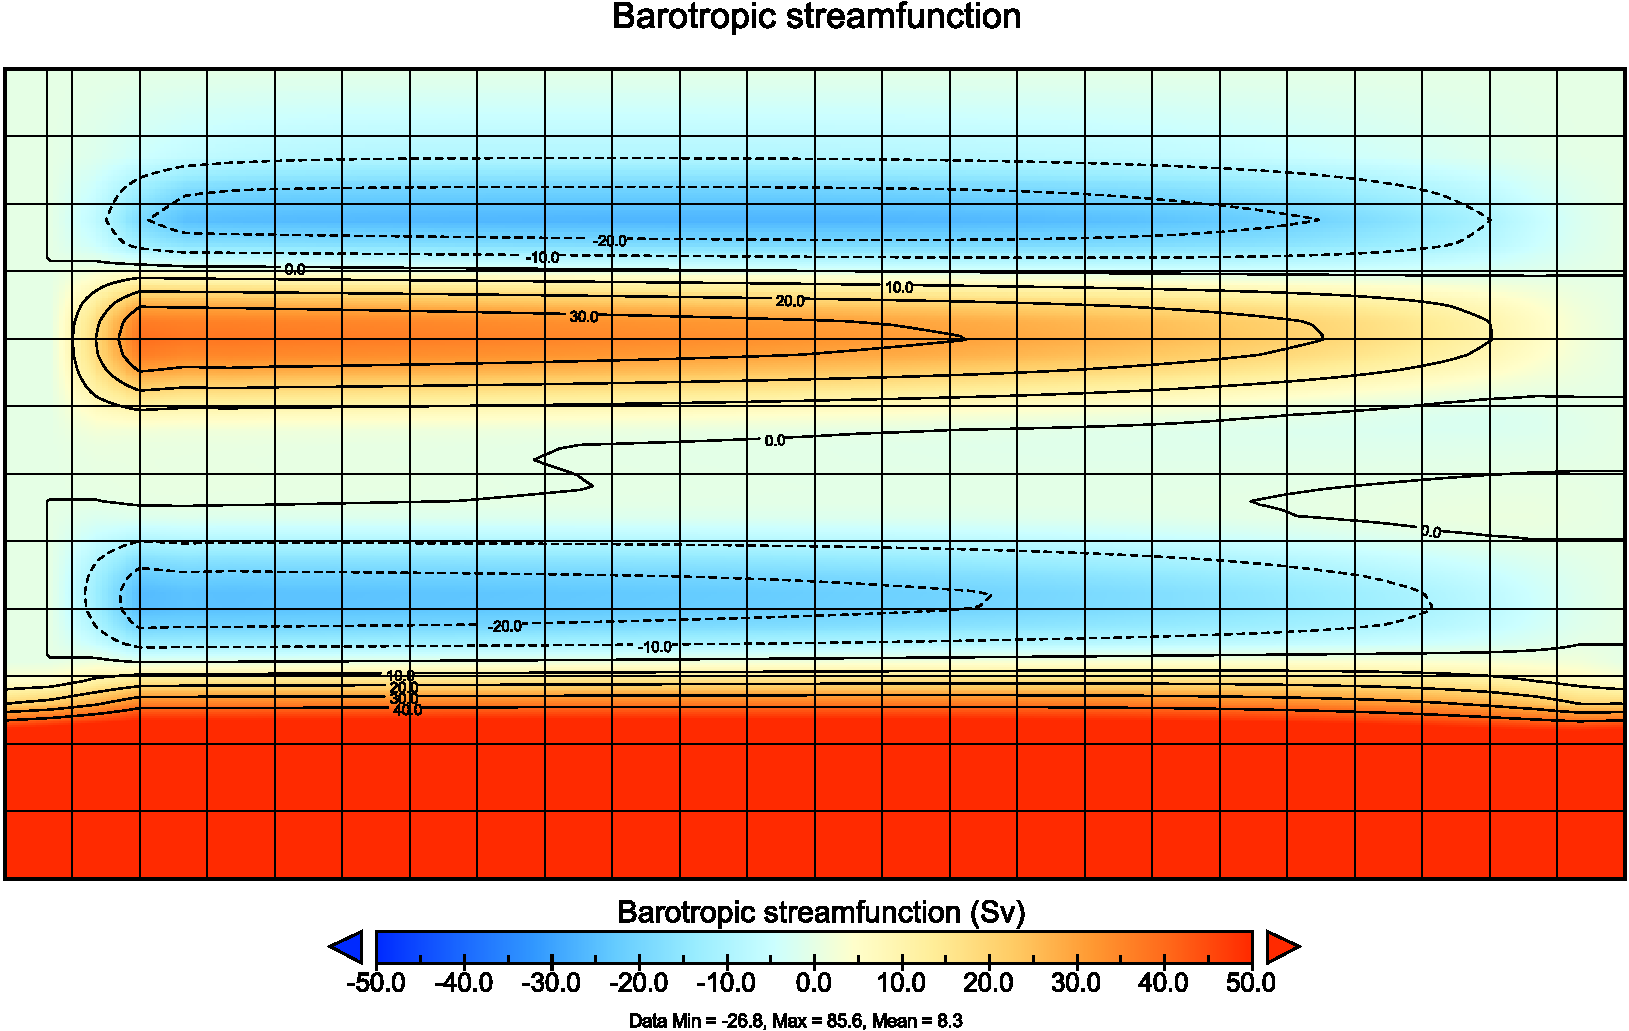
\includegraphics[width=0.5\textwidth]{paleo_drakeworld_psi.pdf}\centering
\vspace{-6mm}
\caption{Drakework world barotropic circulation.}
\label{fig:paleo_drakeworld.psi}
\end{figure}

%------------------------------------------------

\subsubsection{Using MATLAB ...}

\vspace{1mm}
\noindent\rule{4cm}{0.5pt}
\vspace{2mm}

\noindent\textcolor{red}{TO COME ...}

\vspace{1mm}
\noindent\rule{4cm}{0.5pt}
\vspace{2mm}

%------------------------------------------------

\subsubsection{Via color tracing}

Numerical color tracers can be used (as you have seen previously) to trace flow-paths. The default \textit{base-config} files provided as part of the \textbf{muffingen} software, define a configuration with only 2 tracers in the ocean -- T and S. To add red and blue dye tracers, in the \textit{base-config} file, find the section marked:

\footnotesize\vspace{-2pt}\begin{verbatim}
# *******************************************************************
# TRACER CONFIGURATION
# *******************************************************************
# the total number of tracers includes T and S
# T and S do not need to be explicitly selected and initialized
# *******************************************************************
# Set number of tracers
GOLDSTEINNTRACSOPTS='$(DEFINE)GOLDSTEINNTRACS=2'
# list selected biogeochemical tracers
# <<<                                                             >>>
# list biogeochemical tracer initial values
# <<<                                                             >>>
# *******************************************************************
\end{verbatim}\vspace{-2pt}\normalsize

\noindent You need to make several (but simple) edits here:

\vspace{4pt}
\begin{enumerate}
\item Firstly, change the number of tracers from \texttt{2} to \texttt{4}, in line:
\small\vspace{-2pt}\begin{verbatim}
GOLDSTEINNTRACSOPTS='$(DEFINE)GOLDSTEINNTRACS=2'
\end{verbatim}\vspace{-2pt}\normalsize
i.e. to make:
\small\vspace{-2pt}\begin{verbatim}
GOLDSTEINNTRACSOPTS='$(DEFINE)GOLDSTEINNTRACS=4'
\end{verbatim}\vspace{-2pt}\normalsize
\item Secondly, you need to list the additional \texttt{list selected biogeochemical tracers}.
\\For this add the following code in place of the (\(<<<\;\;\;\;\;>>>\)) line:
\small\vspace{-2pt}\begin{verbatim}
gm_ocn_select_48=.true.
gm_ocn_select_49=.true.
\end{verbatim}\vspace{-2pt}\normalsize
\item Lastly, under the section \texttt{list biogeochemical tracer initial values}, and in place of the (\(<<<\;\;\;\;\;>>>\)) line:
\small\vspace{-2pt}\begin{verbatim}
bg_ocn_init_48=0.0
bg_ocn_init_49=0.0
\end{verbatim}\vspace{-2pt}\normalsize
\end{enumerate}

To apply a 'red' dye tracer to the ocean, you can employ the same \textit{forcing} as used in the experiments in Chapter 3 -- \texttt{pyyyyz.Fred} and implement this with similar user-config settings:

\small\vspace{-2pt}\begin{verbatim}
#
# --- FORCINGS --------------------------------------------------------
#
bg_par_forcing_name="pyyyyz.Fred"
bg_par_force_point_i=1
bg_par_force_point_j=1
bg_par_force_point_k=1
bg_par_ocn_force_scale_val_48=0.0
\end{verbatim}\vspace{-2pt}\normalsize

However, the specific \texttt{i,j,k} (longitude, latitude, ocean depth layer) model grid locations will depend on the resolution of the World you generated or had adopted, and it may have e.g. 18 or 36 maximum \texttt{i,j} values, and generally, either 8 or 16 maximum depth levels (\texttt{k}). (The values shown would be for the southern and western corner of the grid at the bottom of the ocean ... but note that this location might be land or seafloor in your particular World!)

%------------------------------------------------

\subsubsection{Via age tracing}

Refer to the 'HOW-TO' in the muffin manual -- 'Add a water mass age tracer':

"\textit{Water mass age tracing can be configured quite simply, and with the tracer concentration manipulations carried out automatically, as follows. As \textit{base-config} file with both red and blue color tracers defined is still required, but  rather than have to define and use a set of \textit{forcings} (and associated forcing configuration), a single parameter is added in the \textit{user-config} file:}
\vspace{-2pt}\begin{verbatim}
bg_ctrl_force_ocn_age=.true.
\end{verbatim}\vspace{-2pt}
\textit{This will automatically create the age tracer and additional explicitly output (in netCDF) both the total age of a water parcel, as well as the age relative to the surface (ventilation age). In this methodology, in the netCDF output, the concentration ratio of blue/red, should be 'age' -- the mean time that a parcel of water was last at the surface.}"

Note that an experiment \textit{spin-up} duration of perhaps as much as 10,000 years is required in order to obtain a stable tracing of water mass age.

%----------------------------------------------------------------------------------------
%       CHAPTER 5
%----------------------------------------------------------------------------------------

\cleardoublepage

\chapterimage{oceanacidification.png} % Chapter heading image

\chapter{Fossil fuel CO$_{2}$ and ‘ocean acidification’}\label{ch:fossil-fuel-co2}

\hfill \break

%------------------------------------------------

\newpage

%------------------------------------------------

\section*{Readme}

You will need to download a new \textit{restart} file prior to embarking on the experiments. This pre-industrial spin-up includes a basic ocean (-atmosphere) carbon cycle plus various diagnostic anthropogenic tracers, following \textit{Cao et al.} [2009].

\vspace{1mm}
\noindent To fetch this: change to the \textsf{\footnotesize cgenie\_output} directory, and type:
\vspace{-2mm}
\begin{verbatim}
$ wget http://www.seao2.info/cgenie_output/LAB_3.SPIN.tar.gz
\end{verbatim}
\vspace{-2mm}

\noindent Extract the contents of this archive by typing:
\vspace{-2mm}
\begin{verbatim}
$ tar xfzv LAB_3.SPIN.tar.gz
\end{verbatim}
\vspace{-2mm}
\noindent (and then change directory back to \textsf{\footnotesize genie-main} to run the model)

%------------------------------------------------

\newpage

%------------------------------------------------

\section{Exploring the consequences of fossil fuel CO$_{2}$ emissions}

For the next experiment(s) you can chuck \(CO_{2}\) into the atmosphere, just for the hell of it. As much as you want! Apparently, humans are actually doing this now. Imagine that!

A new \textit{user-config} for \textbf{muffin} -- \footnotesize\textsf{LAB\_3.CO2emissions }\normalsize -- is provided and configured with climate being responsive to any changes in atmospheric \(CO_{2}\) (i.e., it takes account of \(CO_{2}\)-climate feedbacks):
\vspace{-2pt}\begin{verbatim}
# set CO2-climate feedback
ea_36=y
\end{verbatim}\vspace{-2pt}
\noindent Note that although a biological scheme is set up (with the fixation of organic carbon at the surface and sinking into the ocean interior, plus a rate of calcification by plankton at the surface ocean that is responsive to ocean acidification and saturation state (i.e., it takes into account \(CO_{2}\)-calcification feedbacks, which will additionally interact with climate – see \textit{Ridgwell et al.} [2007b, 2009]\footnote{e.g. obtain from http://www.seao2.info/pubs.html}) ...), we will concentrate only on the carbon geochemistry. (A 'biological pump' in the ocean is set up simply to create a modern-like ocean surface carbonate chemistry. How the biological pump actually operates, response to changes in e.g climate and nutrient availability, we'll consider in another chapter.)

In this \textit{user-config} file, a release of \(CO_{2}\) to the atmosphere is prescribed, which by default is set to a value of just 1 PgC and over an interval of just a single year. (Releasing \(CO_{2}\) just over a single year is obviously rather unrealistic and many impacts will decay away rapidly, but represents a useful idealized experiment for assessing the time-scale(s) of fossil fuel \(CO_{2}\) uptake by the ocean.) Additional (netCDF) output has also been prescribed, via the \textit{user-config} parameter setting: \texttt{bg\_par\_data\_save\_level=10} (see Section 14.4) so that more information relevant to assessing ocean acidification is saved.

\vspace{1mm}
\noindent\rule{4cm}{0.1mm}
\vspace{2mm}

\noindent Run the experiment for e.g., 20 (or more if you like) years, starting from the pre-industrial \textit{re-start} experiment \textsf{\footnotesize LAB\_3.SPIN}, i.e.:
\vspace{-2pt}\begin{verbatim}
$ ./runmuffin.sh cgenie.eb_go_gs_ac_bg.worjh2.BASE LABS
   LAB_3.CO2emissions 20 LAB_3.SPIN
\end{verbatim}\vspace{-2pt}

As for what model results variables to consider … think about the climate change and ocean acidification literature and which environmental (physical and geochemical) properties are considered either critical for ecosystems or are simply helpful and illustrative. Refer to Section 14.6.2 for a summary of some of the key ocean acidification (and other) variables that may be saved by the model\footnote{(depending on specific data saving configuration)}.
In the 3-D netCDF time-slice file remember, for instance, that ocean surface waters in which aragonite becomes under-saturated (OHMEGA < 1.0) is regarded as a critical threshold for organisms making aragonite shells and skeletons and spells TROUBLE for some poor calcifying marine organism somewhere. (Temperature is also highly relevant to marine ecosystems under future global change.) Note that the calcification response is encoded in the model and described in \textit{Ridgwell et al.} [2007a,b] and may or may not reflect the Real World.

For climate change ... the variables of particular interest should be obvious. Remember that there are both \textit{time-series} outputs, as well as  2D and 3D fields, any or all of which might be  helpful for elucidating impacts.

%------------------------------------------------

\subsection{Idealized emissions forcing}

\noindent You can easily modify the experimental design to release more/less \(CO_{2}\) very much as you did for the red dye tracer. In the \textit{user-config} file, the line:
\vspace{-2pt}\begin{verbatim}
bg_par_atm_force_scale_val_3=8.3333e+013
\end{verbatim}\vspace{-2pt}
scales the time-history of the  \(CO_{2}\) flux, given in the forcing file:

\vspace{2pt}
\noindent \footnotesize\textsf{biogem\_force\_flux\_atm\_pCO2\_sig.dat}\normalsize
\vspace{2pt}

\noindent ... which can be found in the directory:

\vspace{2pt}
\noindent \footnotesize\textsf{cgenie.muffin/genie\_forcings/pyyyyz.FpCO2\_Fp13CO2}\normalsize
\vspace{2pt}

\vspace{2pt}
\noindent The format of this file is:
\vspace{-2pt}\small\begin{verbatim}
-START-OF-DATA-
     0.0  1.0
     1.0  1.0
     1.0  0.0
999999.9  0.0
-END-OF-DATA-
\end{verbatim}\normalsize\vspace{-2pt}

\noindent and defines an emission of \(1 mol C\) (carbon) per year over the first year (year 1.0) of the model experiment (between year \texttt{0.0} and \texttt{1.0}), but which in the example \textit{user-config} is then scaled by a value of \(8.333\times10^{13}\) (by the parameter \texttt{bg\_par\_atm\_force\_scale\_val\_3}) to give a total of \(1 PgC yr^{-1}\). (Year 999999.9 has no special meaning and is simply just waaaaay into the future …)

Pause … and note briefly how the final \(CO_{2}\) flux is arrived at. \textbf{muffin} calculates it by multiplying the value in the forcing file (1.0) by a modifying parameter in the \textit{user-config} file (\texttt{8.3333e+13}). The total flux is hence: \(1.0 \times 8.333\times10^{13} = 8.333\times10^{13} mol CO_{2} yr^{-1}\). If you set both values as \texttt{1.0}, you’d get very little carbon released (a single mol!). If you screw up and multiply \texttt{8.3333e+013} and \texttt{8.3333e+013} together as the total flux ... you’ll soon know it as you cook the Earth … But it does not matter which parameter has value \texttt{1.0} and which scales the units (\texttt{8.3333e+013}). For now, it is simply more convenient to be able to edit the \textit{forcing} file with 'simple' numbers (and leave the large numbers and units conversion in the \textit{user-config} file).

Together, the scaling and forcing value gives a \(CO_{2}\) release of \(1 PgC yr^{-1}\) for just a single year compared to current emissions are about \(10 PgC yr^{-1}\). So, do not expect anything exciting if all you emit to the atmosphere is a single measly \(1 PgC\).

(The parameter: \texttt{bg\_par\_atm\_force\_scale\_val\_4=-27.0} specifies the carbon isotopic composition of fossil fuel carbon and can be ignored for now.)

\vspace{1mm}
\noindent\rule{4cm}{0.1mm}
\vspace{2mm}

\noindent Because ‘accidents can happen’ and the global environmental changes induced by the massive fossil fuel \(CO_{2}\) release can obscure mistakes made in the experiment configuration (parameter values) and/or the \textit{re-start} used, you are strongly advised to first (or in parallel, as a job submitted to the cluster – refer to Lesson Zero to remind yourself of the commend line syntax needed for this) --  and \uline{run a control experiment}:
\vspace{-2pt}\begin{verbatim}
$ ./runmuffin.sh cgenie.eb_go_gs_ac_bg.worjh2.BASE LABS
   LAB_3.CONTROL 20 LAB_3.SPIN
\end{verbatim}\vspace{-2pt}
Here – the \textit{user-config} defining the control experiment (\texttt{LAB\_3.CONTROL}) is \uline{identical} to that for the actual experiment itself (\texttt{LAB\_3.CO2emissions}) \uline{with the exception of} the scaling of the \(CO_{2}\) emissions that is set to zero. Note that it is left completely to you to create the experiment configuration file \texttt{LAB\_3.CONTROL} ...

If everything is OK with the control experiment, atmospheric \(CO_{2}\) (and climate) following on from the \textit{re-start} should be stable and there should be little (or no) drift in any of the output variables (because the \textit{spin-up} you are re-starting from should have been run to an equilibrium state and you have not changed anything in the control experiment, right?).

It is good practice (i.e., do it!) to \uline{always run a control experiment} for each different type of experiment – e.g., you only need to run one control experiment for a set \(CO_{2}\) emissions experiments differing only in total carbon release of the time-history of that release.

When you have run both the real and control experiment, compare the results. View (or plot) both relevant \textit{time-series} output, and create anomaly maps of key \textit{time-slice} variables in \textbf{Panoply} or \textbf{MATLAB}, using a corresponding \textit{time-slice} from the control experiment to create the experiment anomaly with.

\vspace{1mm}
\noindent\rule{4cm}{0.1mm}
\vspace{2mm}

\noindent OK. You might want to run something a little more exciting now. For instance, rather than
\vspace{-2pt}\small\begin{verbatim}
-START-OF-DATA-
     0.0  1.0
     1.0  1.0
     1.0  0.0
999999.9  0.0
-END-OF-DATA-
\end{verbatim}\normalsize\vspace{-2pt}
you might have:
\vspace{-2pt}\small\begin{verbatim}
-START-OF-DATA-
     0.0  1000.0
     1.0  1000.0
     1.0     0.0
999999.9     0.0
-END-OF-DATA-
\end{verbatim}\normalsize\vspace{-2pt}
for a total of \(1000 PgC\) is released over a single year. Now you should see some policy-relevant impacts occur :o)

\noindent (Again, contrast control and experiment results to quantify/visualize the impacts of the \(CO_{2}\) release.)

\vspace{1mm}
\noindent\rule{4cm}{0.1mm}
\vspace{2mm}

\noindent You can control the shape of the emissions profile as well as it magnitude. Between the start and end ‘tags’ in the text \textit{forcing} file, the data is arranged into 2 columns: the first contains a series of tie-points for defining the timing of changes in emissions, and the 2nd column contains flux information (units of \(PgC yr^{-1}\) when scaled by the parameter parameter \texttt{bg\_par\_atm\_force\_scale\_val\_3} in the \textit{user-config}). At each time-step of the model, the \(CO_{2}\) flux to be applied to the atmosphere is interpolated between these time points.

For instance, in the \textit{forcing} (directory) file \footnotesize\textsf{biogem\_force\_flux\_atm\_pCO2\_sig.dat}\normalsize, the purpose of:
\vspace{-2pt}\small\begin{verbatim}
     0.0  1.0
     1.0  1.0
     1.0  0.0
999999.9  0.0
\end{verbatim}\normalsize\vspace{-2pt}
is to specify a uniform flux of 1.0 (scaled to \(PgC yr^{-1}\)) over the first full year of the model run, followed by a sharp turn-off to zero flux at the end of first year (and remaining zero thereafter). To extend the period of emissions – for example:
\vspace{-2pt}\small\begin{verbatim}
     0.0  1.0
    10.0  1.0
    10.0  0.0
999999.9  0.0
\end{verbatim}\normalsize\vspace{-2pt}
would result in a uniform flux lasting 10 years with a sudden cut-off and zero thereafter (i.e., once scaled by the parameter in the \textit{user-config} – \(1 PgC yr^{-1}\) over 10 years – \(10 PgC\) total emissions). In contrast:
\vspace{-2pt}\small\begin{verbatim}
     0.0  0.0
    10.0  1.0
    10.0  0.0
999999.9  0.0
\end{verbatim}\normalsize\vspace{-2pt}
would result in a linear ramp, starting from zero at the start of year \(0.0,\) to \(1.0 PgC yr^{-1}\) at year \(10.0\) and then suddenly ceasing and remaining at zero for the remainder of the experiment (a total \(CO_{2}\) emission of \(1\times1.0\times0.5 = 5PgC\) over 10 years).

To ramp up (over 10 years), and then down again (over 10 years), you would specify:
\vspace{-2pt}\small\begin{verbatim}
     0.0  0.0
    10.0  1.0
    20.0  0.0
999999.9  0.0
\end{verbatim}\normalsize\vspace{-2pt}

Make up a few 'shapes' (and hence different experiments), maybe for the same integrated/total emissions, explore the effect of different rates of rise/fall in the release rate. And/or for the same release rate and/or duration, explore the impact of different total emissions of \(CO_{2}\). Try and think in terms of hypotheses and formulate questions to guide your experimental design/configuration. (An alternative approach is to create random scenarios and in the analysis, fish for interesting patters that could lead to knowledge and/or specific questions to be tested further, but it is better to start off with a hypothesis in mind.)

Note that you can either edit and re-use the same \textit{forcing} directory and name, modifying the file \footnotesize\textsf{biogem\_force\_flux\_atm\_pCO2\_sig.dat }\normalsize each time but then losing an explicit record of how you might have set the emissions profile previously, or you can copy and rename the entire \textit{forcing} directory (and then edit \footnotesize\textsf{biogem\_force\_flux\_atm\_pCO2\_sig.dat }\normalsize). If you copy and rename the entire \textit{forcing} directory, in the \textit{user-config}, you then need to specify this new forcing (directory) name, e.g.:
\vspace{-2pt}\begin{verbatim}
# specify forcings
bg_par_forcing_name="pyyyyz.FpCO2_Fp13CO2.NEW"
\end{verbatim}\vspace{-2pt}
if you, for instance, called your new \textit{forcing} directory (in \footnotesize\textsf{genie-forcings }\normalsize): \footnotesize\textsf{pyyyyz.FpCO2\_Fp13CO2.NEW}\normalsize.\footnote{Refer to the directory map in Figure 1.1. if in doubt here.}

\vspace{20pt}

%------------------------------------------------

\newpage
\subsection{Historical (real-world!) emissions forcing}

Historical and future (e.g. IPCC 'SRES') emissions scenarios can also be prescribed explicitly. An example is given as \textit{user-config} file: \textsf{\footnotesize LAB\_3.historical}. In this, a historical emissions forcing (technically: a prescribed concentration profile of p\(CO_{2}\) and other anthropogenic gases) is specified by the \textit{forcing}:
\vspace{-2pt}\begin{verbatim}
bg_par_forcing_name=’worjh2.historical2010’
\end{verbatim}\vspace{-2pt}
In contrast to before, no additional scaling is needed because the forcing specification directly follows the observed change in atmospheric concentration with time (in units of atm \(CO_{2}\)).

An additional line appears in the \textit{user-config} because the historical p\(CO_{2}\) transient starts in the 1700s (for which a nominal date of 1765 is often used) rather than year zero. For example, to start \textbf{muffin} from year 1765 rather than zero, the start year parameter is set thus:
\vspace{-2pt}\begin{verbatim}
bg_par_misc_t_start=1765.0
\end{verbatim}\vspace{-2pt}
It is also convenient to specify a set of time save points that are consistent with the historical period. In the example \textit{user-config}, the addition of the parameter settings:
\vspace{-2pt}\begin{verbatim}
bg_par_infile_slice_name=’save_timeslice_historicalfuture.dat’
bg_par_infile_sig_name=’save_timeseries_historicalfuture.dat’
\end{verbatim}\vspace{-2pt}
 specifies a series of time points at which data is saved that aligns with historically relevant years.

Try viewing the contents of these (text) files:
\vspace{2pt}
\\ \small\textsf{save\_timeslice\_historicalfuture.dat }\normalsize
\\ \small\textsf{save\_timeseries\_historicalfuture.dat }\normalsize
\vspace{2pt}
\\which can be found in the directory: \footnotesize\textsf{genie-biogem/data/input }\normalsize, to get a sense of how frequently the data will be saved, and how this differs from the default settings, which are defined in the files:
\vspace{2pt}
\\ \small\textsf{save\_timeseries.dat }\normalsize
\\ \small\textsf{save\_timeslice.dat }\normalsize
\vspace{2pt}

A suitable experiment would then be one run for 245 years so that it reaches year 2010 (having started from year 1765):
\vspace{-2pt}\begin{verbatim}
$ ./runmuffin.sh cgenie.eb_go_gs_ac_bg.worjh2.BASE LABS
   LAB_3.historical 245 LAB_3.SPIN
\end{verbatim}\vspace{-2pt}
(Here, the 245 year run duration is simply calculated to get you from year 1765 to 2010 ...)

WARNING! Ignore the ‘WARNING’s at the start -- these are simply telling you that more tracer forcings have been specified than you have selected tracers for in the \textit{base-config}: \\(\textsf{\footnotesize cgenie.eb\_go\_gs\_ac\_bg.worjh2.BASE}). (A different \textit{base-config} with additional selected tracers could have been specified to make use of other historical changes in atmospheric composition, such as of radiocarbon ($^{14}$C) and CFCs.) Also: from year 1765 onwards, changes in atmospheric \(CO_{2}\) only rise very s l o w l y initially. Don’t expect to see anything happen in 10 seconds flat because relatively few people and countries in the 1800s could be bothered to burn much more than a little local coal. You could potentially start your experiment at year 1850, changing the value of \texttt{bg\_par\_misc\_t\_start} and specifying shorter experiment duration if you are desperate for the End of the World to come.

Don’t forget: you could submit this experiment to the cluster and do more (idealized emissions) ‘playing’.

%\vspace{1mm}
%\noindent\rule{4cm}{0.1mm}
%\vspace{2mm}

\noindent Given that there is observationally-based information on the distribution of anthropogenic \(CO_{2}\) taken up by the ocean (e.g., \textit{Sabine et al.} [2004]) ... and you are running a historical transient experiment with the model driven by observed increases in atmospheric p\(CO_{2}\) ... you are in a position to critically evaluate the models ability (or lack of) to represent the future-critical process of oceanic fossil fuel \(CO_{2}\) uptake and transport by large scale ocean circulation.

In the 2D \textbf{netCDF} output, there is a variable for the water column integrated inventory of DIC – equivalent to the Sabine map except you will need to subtract the preindustrial background of DIC first, i.e., to create a DIC anomaly map representing only the added fossil fuel \(CO_{2}\) component of ocean DIC. The data in the Sabine paper clusters around 1994. A \textit{time-slice} centered on this year (1994.5) has been configured in the model exactly for this purpose. Your baseline state can either be from prior to \(CO_{2}\) emissions commencing at any significant rate (e.g., 1750.5) or (better), from a control experiment. Note that similar comparisons could be (and are regularly) made with other tracers such as CFCs, which provide additional insights into the patterns and time-scales of trace gas update and ocean circulation. (See: \textit{Cao et al.} [2009])

Observational data, re-gridded to the \textbf{muffin} grid and in netCDF format can be downloaded from the ‘usual place’ (http://www.seao2.org/mymuffin.html) from the ‘got data?’ box on the left. You could for instance, compare horizontal or vertical slices (3D netCDF) and create difference (anomaly) maps. Somewhat more representative of the entire ocean is to compare (or calculate difference maps) of zonal average profiles. Unfortunately, the observations are not in the form of water column integrals and hence you cannot create difference maps of model as per the \textit{Sabine} paper … unless you are \textbf{MATLAB}-friendly and you use the 3D \textbf{BIOGEM} \textbf{MATLAB} plotting scripts (https://github.com/derpycode/muffinplot) whose use is somewhat described in the \textbf{muffin} user-manual. Examples of \textbf{MATLAB} plotting of the model \textit{vs.} observed anthropogenic anomaly are shown in Figure \ref{fig:chx-co2uptake} (note the use of plotting un-interpolated model grid data as colors but with an interpolated contour overlain to help guide the eye and pick out features).

\begin{figure}[ht]
\begin{center}
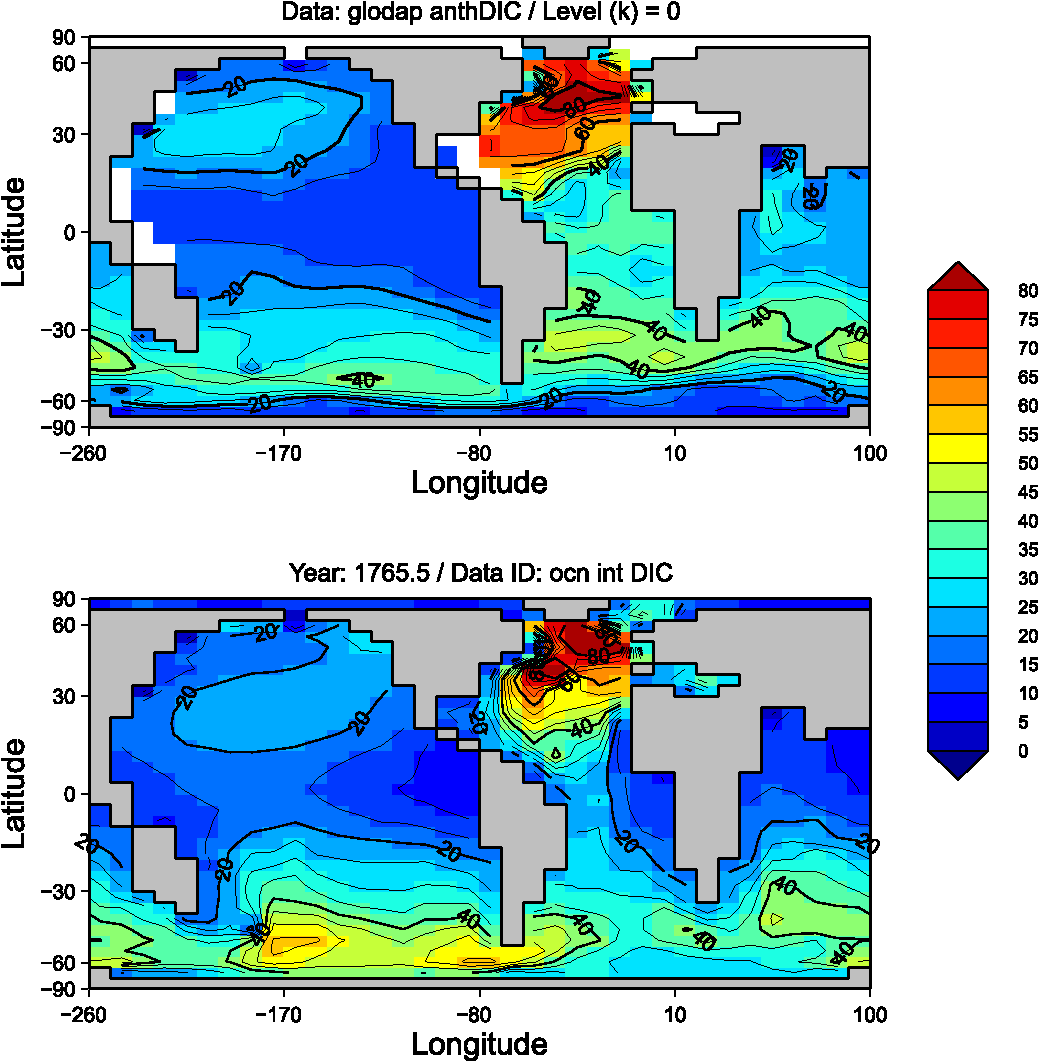
\includegraphics[scale=0.55]{chx-co2uptake.pdf}
\end{center}
\vspace{-10pt}
\caption{Observed (top) \textit{vs.} Model (bottom) anthropogenic \(CO_{2}\) inventories.
Data and model water column integrals in units of mol \(CO_{2}\) m$^{-2}$ and are nominally with respect to year 1994.}
\label{fig:chx-co2uptake}
\end{figure}

\vspace{1mm}
\noindent\rule{4cm}{0.1mm}
\vspace{2mm}

\noindent Finally, and the closest to being slightly interesting: rather than applying highly idealized pulses  of \(CO_{2}\) emissions, the IPCC 'SRES' emissions scenarios can be used to make future projections with. An example forcing of this sort is provided and can be selected by changing the name of the forcing selection parameter (\texttt{bg\_par\_forcing\_name}) to one of the following:
\vspace{-2pt}\begin{verbatim}
pyyyyz.FpCO2_Fp13CO2.A1_AIM
pyyyyz.FpCO2_Fp13CO2.A1G_MINICAM
pyyyyz.FpCO2_Fp13CO2.A1T_MESSAGE
pyyyyz.FpCO2_Fp13CO2.A2_ASF
pyyyyz.FpCO2_Fp13CO2.B1_IMAGE
pyyyyz.FpCO2_Fp13CO2.B2_MESSAGE
\end{verbatim}\vspace{-2pt}
These are 'future' emissions scenarios, which all start at year 2010, and end at year 2100. They are derived from different socio-economic and future technological assumptions in making their future emissions projections.

Again, as these forcings have units of \(PgCyr^{-1}\) in the time-series files, you will need to add a scaling parameter to the \textit{user-config} file to turn units of \(PgCyr^{-1}\) into \(mol C yr^{-1}\), i.e.,
\vspace{-2pt}\begin{verbatim}
bg_par_atm_force_scale_val_3=8.3333e+013
\end{verbatim}\vspace{-2pt}

For complete ‘realism’, you will need to run this experiment starting from the end of the historical transient experiment you have just run (Section 1.6), e.g.,
\vspace{-2pt}\begin{verbatim}
$ ./runmuffin.sh cgenie.eb_go_gs_ac_bg.worjh2.BASE LABS
   LAB_3.future 90 LAB_3.historical
\end{verbatim}\vspace{-2pt}
and with the start from year now set to year 2010 (the end year of the historical transient):
\vspace{-2pt}\begin{verbatim}
bg_par_misc_t_start=2010.0
\end{verbatim}\vspace{-2pt}
Note that the \textit{user-config} \footnotesize\textsf{LAB\_3.future }\normalsize is not provided for you – you will need to create this (or a file named whatever you like) by copying e.g., \footnotesize\textsf{LAB\_3.EXAMPLE }\normalsize and making the parameter changes described above (forcing specification parameter, emissions scaling parameter, and start year parameter).

You can also easily replace the details of the emissions with other SRES scenarios – simply find the year \textit{vs.} emissions rate information from the interweb\footnote{e.g., http://sres.ciesin.columbia.edu/final\_data.html} and edit or copy-and-paste the flux values for each decade into the file \footnotesize\textsf{biogem\_force\_flux\_atm\_pCO2\_sig.dat }\normalsize in the forcing directory.\textbf{ muffin} will then automatically interpolate between the decadal tie-points to give a continuous change in emissions. Now you are able to make a rather more realistic/plausible assessment of when and where potential ecological impacts (via assumed ocean chemistry criteria) might occur.

Try running (e.g. as jobs submitted to the cluster queue), some other actual or made up SRES emissions scenarios.

(Note that the past few IPCC assessment reports have switched to 'using 'RCP's -- Representative Emissions Pathways, rather than the SRES emissions scenarios -- see later Section.)

%------------------------------------------------

\newpage

%------------------------------------------------

\section{Further ideas}

%------------------------------------------------

\subsection{Assessing the importance of emissions rate}

By editing the flux and/or timing information, you can control the \(CO_{2}\) emissions trajectory as well as the total of fossil fuel carbon burned. Explore different \(CO_{2}\) release assumptions and note their differing impact on climate and ocean (carbonate) geochemistry. Much more realistic and appropriate to our \textit{current} global experiment is a lower rate (order of 10 or 20 \(PgCyr^{-1}\)) released over a longer interval (order of 100 years) as compared to a conceptual 1000 \(PgC\) near-instantaneous pulse. Because the experiments are getting longer to run in real time … remember to make appropriate use of the cluster queuing facility – i.e., think about whether you want to sit around starting at the screen for 15 minutes waiting for a new line of numbers appear – if not: submit to the cluster queue. For instance, one might try and address the question: “For a given total release of  fossil fuel \(CO_{2}\), is it safer to burn it slower?” The answer is maybe not completely obvious, as burning carbon resources slower will result in a small global impact, but perhaps one that persists for longer(??). You could conceive of an ensemble (related set) of model experiments, maybe one of 100 \(PgCyr^{-1}\) for 1 yr, one of 10 \(PgCyr^{-1}\) for 10 years, and one of 1 \(PgCyr^{-1}\) for 100 years, and run them all for e.g., 100 years.\footnote{These all represent rather unrealistically small total \(CO_{2}\) releases and you may want ot consider a total more like 1000 \(PgC\) or rather more. You may also want to think about more realistic shapes rather than pulses, such a some sort of ramp up and then down in the emissions rate (but for the same total emissions).} (As jobs submitted to the queue, all can be run simultaneously (with blank spaces between commands!).) (\uline{Don’t forget the control experiment}! (configured the same, except with 0 \(PgCyr^{-1}\) of emissions for 100 years).)

Note note that you should create 3 new \textit{forcings} based on the original if you are editing the same original  \textit{forcing} and expecting to run different ones at the same time. Really, this is little more than you did in copying and renaming \textit{user-config} files in order to create new experiments ... except that now it involves copying and renaming entire directories in \textsf{\footnotesize genie-forcings}. Remember that the \textit{forcing} is specified by the directory name assigned to \texttt{bg\_par\_forcing\_name} (enclosed in \texttt{''}) and you will need to change this to match the name of your new \textit{forcing} directory.

%------------------------------------------------

\subsection{Determining thresholds of environmental impact}

There are various concerns about the impacts of continuing fossil fuel \(CO_{2}\) emissions and a number of proposed climatic (e.g., the 2 degree C global warming limit often mentioned in policy documents) and ecological ‘tipping points’. You can assess the maximum allowable \(CO_{2}\) emissions to remain within particular global environmental limits in the model. For example:

\begin{itemize}[noitemsep]

\vspace{1mm}
\item What is the maximum total \(CO_{2}\) release that can be made without inducing aragonite under-saturation at the ocean surface anywhere (or any season – see Section 5.2.3 in the User Manual for seasonal time-slice data saving)? How important is the time-scale of emissions in determining this? For total emissions above this: where in the ocean does the surface first become under-saturated and what sort of (calcifying) organisms might be impacted there? How large would the emissions have to be in order to start to induce under-saturation with respect to aragonite at the surface in the tropics (home to socio-economically important reef systems)? These are questions that can be addressed with simple \(CO_{2}\) release experiments in ocean carbon cycle models and everyone seems to get a GRL paper out of it each and every time!

\vspace{1mm}
\item How important are \(CO_{2}\)-climate feedbacks in amplifying or diminishing future climate and ocean carbonate chemistry changes – e.g., is the same atmospheric p\(CO_{2}\) value reached with and without climate feedback (and surface warming) – if not, why? 

Hint: the solubility of \(CO_{2}\) in sea-water is a function of temperature and at higher temperatures, \(CO_{2}\) is less soluble. This means that with climate warming, \(CO_{2}\) solubility declines, less is taken up by the ocean and more is left in the atmosphere -- driving further heating in a \uline{positive feedback}.

\vspace{1mm}
All your \(CO_{2}\) emissions experiments to date have had this feedback enabled -- specified at the top of the \textit{user-config} file by:
\vspace{-2pt}\small\begin{verbatim}
# set climate feedback
ea_36=y
\end{verbatim}\normalsize\vspace{-2pt}

To quantify the role of the carbon-climate feedback, you need to run an identical emissions experiment, but with the feedback disabled:
\vspace{-2pt}\small\begin{verbatim}
# set climate feedback
ea_36=n
\end{verbatim}\normalsize\vspace{-2pt}

Note that you also to need to run a historical transient experiments with no carbon-climate feedback, if you are starting emissions experiments from the year 2010. i.e. you will have a set of future emissions experiments including the carbon-climate feedback that are run from a historical transient experiments that also includes carbon-climate feedback, vs. a set of future emissions experiments without the carbon-climate feedback that are run from a historical transient experiments that also \uline{does not include} carbon-climate feedback.

The importance of the feedback is simply the difference between the 2 sets of experiments, at the same year.

\vspace{1mm}
\item Also: How much \(CO_{2}\) emission does it take to significantly ‘collapse’ the AMOC and over what time-scale? (Or alternatively: what is the atmospheric p\(CO_{2}\) threshold for collapse?)
\\ If the AMOC weakens or collapses … why in the absence of a prescribed freshwater perturbation does this happen? What physical process are at play in response to rapid \(CO_{2}\) release too the atmosphere that may act to reduce or shutdown deep-water formation in the ocean model? (Plotting appropriate ocean property anomalies between the \(CO_{2}\) release experiment and a control experiment might help.)
\\Related to a previous possible investigation -- does the rate of \(CO_{2}\) increase (for the same total release) matter? If so, why? What is happening in general to the structure and dynamics of the upper ocean when surface warming is very rapid?

\end{itemize}

\vspace{1mm}
\noindent Experiments could be hypothetical and consisting of \(CO_{2}\) pulses or ramps (or exponentials) and run on directly from a pre-industrial spin-up, or more ‘realistic’ and run on from the end of a historical transient experiment (e.g., starting in year 2010).

\noindent Also:

\begin{itemize}[noitemsep]

\vspace{1mm}
\item How much carbon can  be burned (and how quickly) such that atmospheric \(pCO_{2}\) does not increase any further and remains at some specific value (you might pick \(\times2\) or \(\times4\) preindustrial \(pCO_{2}\) (ca. 278 ppm))? This is difficult to determine well because to hold atmospheric \(pCO_{2}\)  constant, continuing emissions are required (as \(CO_{2}\) continues to be taken up by the ocean).
\vspace{1mm} 
\\One possible approach to tacking this, might be:
\vspace{1mm} 
\begin{enumerate}[noitemsep]
\item Run one or more (SRES) emissions scenarios and find the year at which your \(pCO_{2}\) threshold value is crossed. 
\item Re-run the same emissions experiment, but only for as many years as the threshold-crossing year you had identified, is reached. This will become your new \textit{re-start} experiment.
\item Create a new experiment, with zero emissions, and run on from your new re-start. You should see atmospheric \(pCO_{2}\) start close to the value you reached at the end of the last experiment, but then decay away as the ocean continues to absorb carbon from the atmosphere. The decline in atmospheric \(pCO_{2}\) each year tells you something about the yearly emissions needed to keep atmospheric \(pCO_{2}\) constant.
\\An approximate rule-of-thump, is that \(1ppm\) in atmospheric \(pCO_{2}\) is equivalent to \(2 PgC\) (actually, a more exact conversion is \(1 ppm = 2.123 PgC\)). So you could calculate a yearly time-series of how much (in ppm) atmospheric \(pCO_{2}\) falls by each year ... convert this to PgC, and then create a new \textit{forcing}, with this as the annual emissions.
\item Create and run a new experiment, from the same \textit{re-start} experiment you created, and apply the new emissions forcing you created. See if atmospheric \(pCO_{2}\) is approximately maintained constant(?)  
\item If not sufficient constant to your satisfaction, you could also carry out a second iteration -- calculating from your latest experiment, the ppm change in \(pCO_{2}\) each year, converting to an emissions rate, and running a further experiment ...
\\Note that if you 'overhsoot' and \(pCO_{2}\) rises above the threshold value rather than falls below, you are allowed to have a \uline{negative} carbon emission to the atmosphere in your forcing.
\item The sum of the carbon emissions up to the threshold being reached, is your answer to how much more carbon can be burned and not cross that threshold ... but you will see that after that, further emissions are allowed without \(pCO_{2}\) exceeding the threshold. So the answer e.g. for year 2100 (or 2200) will be larger.
\end{enumerate}

\vspace{1mm} 
There are automated ways provided in the model framework of  achieving this, and you can for instance simply tell \textbf{muffin}  to maintain a specific (or changing) value of atmospheric \(pCO_{2}\), and from this diagnose the emissions rate that was required. For instance, you'll see in the original \textit{re-start} \textit{user-config} for this chapter -- \textsf{\footnotesize LAB\_3.SPIN} -- the \textit{forcing} used is 
\textsf{\footnotesize worjh2.preindustrial}, and if you go an look in that forcing directory:
\vspace{1mm}
\\\textsf{\footnotesize biogem\_force\_restore\_atm\_pCO2\_sig.dat} 
\vspace{1mm}
\\you will see that this basically requests that atmospheric \(pCO_{2}\) is held at \(278 ppm\) (\(0.278\times10^{-6} atm\)). You could then copy and rename this \textit{forcing}, and change:
\vspace{-2pt}\small\begin{verbatim}
0.0      278.0E-6
999999.0 278.0E-6
\end{verbatim}\normalsize\vspace{-2pt}
to:
\vspace{-2pt}\small\begin{verbatim}
0.0      556.0E-6
999999.0 556.0E-6
\end{verbatim}\normalsize\vspace{-2pt}
(in the case of a \(\times2\) preindustrial \(pCO_{2}\) threshold). \textbf{muffin} will then attempt to maintain \(pCO_{2}\) at this specified value. The equivalent carbon emissions required to do this, are diagnosed and provided as a \textit{time-series} output (in units of \(mol C yr^{-1}\)) in file: \\\textsf{\footnotesize biogem\_series\_diag\_misc\_specified\_forcing\_pCO2.res}

\vspace{1mm}
\item Similarly -- how much more carbon can be burned but still keep global mean surface air temperature from rising beyond the 'Paris' limit of \(2^{\circ}C\) (as compared to preindustrial)?
\\This is also difficult to determine well because there are significant climate lags in the system with warming continuing even if atmospheric \(pCO_{2}\) was held constant.
\\Trial-and error would be one approach ...

\end{itemize}

%------------------------------------------------

\subsection{Future atmospheric CO$_{2}$ concentration pathways ('RCPs')}

The more recent/current incarnation of IPCC future scenarios revolves not around  making projections of future greenhouse gas emissions rates, but rather future greenhouse gas concentration pathways. (The reasoning is partly to cut out the differences in carbon cycle feedback between models, where for the same unit \(CO_{2}\) release, different climate/Earth system models might project a different atmospheric \(CO_{2}\) concentration and hence climate change (in addition to differences between models in climate sensitivity).) In muffin, these work pretty well much like in the historical forcing scenario, where the observed change in atmospheric \(CO_{2}\) concentration in the atmosphere with time, is prescribed and the model 'forced' to conform to this trajectory.

A series of RCP scenarios for how atmospheric \(CO_{2}\) concentrations may evolve with time are provided. Each actually starts at year 1765 and hence incorporates the historical transient. They can hence be used with an experiment starting at 1765 and \textit{re-starting} from a steady-state preindustrial \textit{spin-up}. Or they can be jumped into at ay point, and e.g. experiments started at year 2010, when only the year 2010 onwards part of the \(CO_{2}\) restoring \textit{forcing} is utilized. The RCP \textit{forcings} currently provided are:

\vspace{2pt}
\begin{itemize}[noitemsep]
\setlength{\itemindent}{.2in}
\item \textsf{\footnotesize pyyyyz.RpCO2\_Rp13CO2.RCP3PD}
\item \textsf{\footnotesize pyyyyz.RpCO2\_Rp13CO2.RCP4p5}
\item \textsf{\footnotesize pyyyyz.RpCO2\_Rp13CO2.RCP6p0}
\item \textsf{\footnotesize pyyyyz.RpCO2\_Rp13CO2.RCP8p5}
\end{itemize}
\vspace{2pt}

\noindent and can be selected simply by changing the name of the forcing in the \textit{user-confi}g, e.g.:
\vspace{-2pt}\begin{verbatim}
bg_par_forcing_name=’pyyyyz.RpCO2_Rp13CO2.RCP8p5'
\end{verbatim}\vspace{-2pt}
\noindent which would select the RCP8.5 scenario.

\vspace{1mm}
\noindent \uline{NOTE}: ensure that
the scaling parameters are either commented out, e.g.:
\vspace{-2pt}\small\begin{verbatim}
#bg_par_atm_force_scale_val_3=8.3333e+013
#bg_par_atm_force_scale_val_4=-27.0
\end{verbatim}\normalsize\vspace{-2pt}
\noindent or simply deleted in their entirety (because the RCP forcing contains the actual values/correct units and you do not need to modify them any further).

The equivalent carbon emissions required to follow these concentration pathways are diagnosed by \textbf{muffin} and provided as a \textit{time-series} output (in units of \(mol C yr^{-1}\)) in file: 
\vspace{1mm}
\\\textsf{\footnotesize biogem\_series\_diag\_misc\_specified\_forcing\_pCO2.res}

%------------------------------------------------

\subsection{Isotopic tracing of fossil fuel CO$_{2}$ uptake}

See: 12.2.1

%----------------------------------------------------------------------------------------
%       CHAPTER X
%----------------------------------------------------------------------------------------

\cleardoublepage

\chapterimage{chx-biogeo.png} % Chapter heading image

\chapter{Ocean biogeochemical cycles}\label{ch:ocean=biogeochem}

\hfill \break

\vspace{24mm}

\noindent

%------------------------------------------------

\newpage

%------------------------------------------------


\section*{READ.ME}

You will need the following \textit{re-starts} files prior to embarking on the experiments in the Chapter.
\vspace{1mm}

\begin{itemize}[noitemsep]
\vspace{1mm}
\item [7.2] This is of a basic single (\(PO_{4}\)) nutrient biological export scheme.
\small \begin{verbatim}
$ wget http://www.seao2.info/cgenie_output/EXAMPLE.worbe2.Ridgwelletal1997.SPIN.tar.gz
\end{verbatim} \normalsize
\vspace{1mm}
\item [7.3] 
\small \begin{verbatim}
...
\end{verbatim} \normalsize
\vspace{1mm}
\item [7.4] 
\small \begin{verbatim}
$ wget http://www.seao2.info/cgenie_output/201015.ENS.solscav6x6c.00.tar.gz
\end{verbatim} \normalsize
\vspace{1mm}
\item [7.5] 
\small \begin{verbatim}
$ wget http://www.seao2.info/cgenie_output/LAB_4.SPIN.tar.gz
\end{verbatim} \normalsize
\end{itemize}
\vspace{1mm}

\noindent Extract the results in the usual way and in the usual place ... and return to \textsf{\footnotesize genie-main} in the usual way ... all ... as usual.

%------------------------------------------------

\newpage

%------------------------------------------------

\section{The ocean's biological pump}

In this Chapter we'll step through some of the facets of the cycle of carbon (and nutrients) in the ocean -- the 'biological pump'. (And then in the following section we'll look at the same processes in a different way via 'geoengineering' and hopefully learn something further about how it all  'works'.)

\textbf{muffin} incorporates a variety of options for simulating biological export production. To date, these have all been rooted in what is effectively a nutrient mass balance approach to estimating export production, nicely encapsulated by Ernst Maier-Reimer as: “conceptually not a model of biology in the ocean but rather a model of biogenically induced chemical fluxes [from the surface ocean]” [\textit{Maier-Reimer,} 1993]. Hence in schemes of this nature, which we will term ‘biogenic export’, there is no attempt to explicitly account for changes in cell numbers/biomass and hence, nor zooplankton, which will impact a bias particularly in the seasonal time-dependent response of export. Previous biogenic export schemes utilized in  \textbf{muffin}  considered a single nutrient (P limitation) only and took either restoring to observations [Cameron et al., 2005] or explicit P-limitation [Ridgwell et al., 2007a,b] approaches. More recently, additional limitation by iron (P+Fe) has been implemented, while nitrogen cycling (including N fixation and denitrification) and hence P+N limitation, has been implemented and explored in the context of extreme nutrient and oxygen cycle perturbation associated with the Cretaceous Oceanic Anoxic Events [Monteiro et al., 2012; Naafs et al., 2029]. Work currently in development includes the additional consideration of Si limitation (P+Si limitation) control on production of diatoms vs. non-diatoms following \textit{Ridgwell et al.} [2002].

Overall, biological production and net export of particulate (POM) and dissolved (DOM) organic matter plus calcium carbonate (\(CaCO_{3}\)) are directly determined by the availability of nutrients (phosphate and/or total dissolved iron and/or \(NO^{2-}_{3}\) (and/or \(NH^{+}_{4}\)) and/or dissolved silica) together with the degree to which physical conditions, particularly light and temperature, are conducive to growth. DOM is remineralzied (transformed back to inorganic dissolved constituents) relatively rapidly (a ca. annual time-scale) and hence mostly at or close to the ocean surface, while POM is assumed to sink down into the ocean interior. See: \textit{Hülse at al.} [2017]\footnote{Hülse, D., S. Arndt, J.D. Wilson, G. Munhoven, and A. Ridgwell, Understanding the causes and consequences of past marine carbon cycling variability through models, Earth-Science Reviews 171, dx.doi.org/10.1016/j.earscirev.2017.06.004 (2017).} for a comprehensive review (esp. of implementation in models).

Note that a full description of the various biological and ocean interior remineralization schemes (together constituting the biological pump) is not given here as background. Rather, \uline{the relevant provided references should be read} (rather than e.g. downloaded and forgotten ...).

%------------------------------------------------

\newpage

%------------------------------------------------

\section{Single nutrient (PO$_{4}$) cycling and basic controls on biological productivity}

The following exercises  will utilize one of the more basic representations of the biological pump -- one with only a single nutrient (PO$_{4}$) potentially limiting to biological export, considered. The scheme is described in full in \textit{Ridgwell et al.} [2007]\footnote{Ridgwell, A., et al., Marine geochemical data assimilation in an efficient Earth System Model of global biogeochemical cycling, Biogeosci. 4, 87-104 (2007). }.We will consider the following scientific questions as a starting point and then devise some model experiments to address them:

\begin{enumerate}[noitemsep]
\vspace{1mm}
\item What would the Earth look like with no biological production in the ocean? Specifically: how important is the biological pump in controlling atmospheric \(pCO_{2}\) and how much higher would \(pCO_{2}\) be in the absence of a biological pump in the ocean?
\vspace{1mm}
\item Conversely, is the biological pump operating at its maximum efficient in the ocean today, and if not, how much more could atmospheric \(pCO_{2}\) conceivably be lowered.
\vspace{1mm}
\item How does the biological pump affect the distribution and hence availability of dissolved oxygen in the ocean? (How more oxygenated would the ocean be with no export of organic matter into the ocean interior, and how much more severe would oxygen depletion be if plankton were able to utilize all the nutrients at the ocean surface?)
\vspace{1mm}
\item If carbon and nutrients are returned back to solution (remineralized) much closer to the ocean surface, does atmospheric \(pCO_{2}\) increase or decrease?? (The faster return of DIC to the ocean surface will tend to increase \(pCO_{2}\) while the return of nutrients will tend to enhance biological productivity and decrease \(pCO_{2}\) ...)
\vspace{1mm}
\item What about if carbon and nutrients are much more efficiently exported into the very deepest parts of the ocean -- does \(pCO_{2}\) increase or decrease (and what happens to e.g. \([O_{2}]\))?
\vspace{1mm}
\item What is the role of the calcium carbonate (\(CaCO_{3}\)) 'counter pump'? How much higher is \(pCO_{2}\) in the presence of calcifying organisms in the ocean compared to just organic matter production and cycling?
\vspace{1mm}
\item What about feedback with climate -- how does changing global surface temperature (and hence ocean circulation patterns and sea-ice extent) modulate the impact of changes to the biological pump in the ocean? Is the resulting feedback positive or negative (and why)?
\end{enumerate}
\vspace{1mm}

The associated experiments would ideally be run for several thousand and maybe 5000 years to obtain a new (quasi) steady state of carbon and nutrient cycling in the ocean. But some of the impacts in the ocean and on atmospheric \(pCO_{2}\) will develop relatively rapidly (decades). Hence model experiments could be run for a few 10s of years, or e.g. 100 years, or for a full e.g. 5000 years but periodically downloading and viewing the results as the experiment progresses (and not necessarily waiting until the end of the experiment, or even ever looking at the final state!).

All the experiments will start from the same \textit{re-start}\footnote{As per described in Ridgwell et al. [2007].} and will be based on the same \textit{user-config}\footnote{The same \textit{user-config} as used to generate the \textit{re-start} (with the exception that the atmospheric \(CO_{2}\) concentration is no longer prescribed).} (and note the use of a different \textit{base-config} to previously):
\vspace{-2mm}\begin{verbatim}
./runmuffin.sh cgenie.eb_go_gs_ac_bg.worbe2.BASES LABS EXP.7.2
 5000 EXAMPLE.worbe2.Ridgwelletal1997.SPIN
\end{verbatim}\vspace{-2mm}
(here a 5000 year experiment run-time is given, but it need not be this -- see above). Remember to copy and rename \textsf{\footnotesize EXP.7.2} in order to create new and unique experiments each time.

\pagebreak

The first thing to do, is to run an control experiment, for however long you have decided to run all the actual experiment experiments for. (You need not wait for this to finish, but can submit it as a \textit{job} to the cluster and get on with running some real experiment experiments.) The control experiment can simply be derived (copied) from \textsf{\footnotesize EXP.7.2}, with no further alterations needed. In this \textit{user-config}, the value of atmospheric  \(pCO_{2}\) is not prescribed (there is no \textit{forcing} defined) and hence \(pCO_{2}\) is free to respond to any change in parameters. In the case of the control -- there are no changes in the biological pump parameters compared to the \textit{spin-up}, so you should see no (or little) drift in \(pCO_{2}\) occurring.

Also think about the output you want to view (and how to view it). You are likely to want to look at anomalies vs. the control, as well as absolute patters in the ocean. In the \textit{user-config} -- check that the results/output select 'level' is going to give you the output you are expecting. This is parameter:
\vspace{-1mm}\small\begin{verbatim}
bg_par_data_save_level=5
\end{verbatim}\normalsize\vspace{-1mm}
Refer to Section 14.4 and Appendix I, for more details on how different (2D and 3D) \textit{time-slice} variable fields and \textit{time-series} are selected to be included in the model ouptut. 

\vspace{2mm}
\noindent In terms of the specific 'questions' above (the numbering system is the same), both w.r.t. what parameters and parameter values to change and well as what to 'look for':

\begin{enumerate}[noitemsep]

\vspace{1mm}
\item The parameter scaling the rate of nutrient uptake (and hence biological export) is:
\vspace{-1mm}\small\begin{verbatim}
# maximum rate of conversion of dissolved PO4 into 
# organic matter by phytoplankton (mol kg-1 yr-1)
bg_par_bio_k0_PO4=1.9582242E-06
\end{verbatim}\normalsize\vspace{-1mm}
(in units of \(mol\:PO_{4} \:kg^{-1} \:yr^{-1}\)). Setting this to zero would 'turn off' completely the biological pump, leaving you with a abiotic ocean.
\\What to look for? The value of atmospheric \(pCO_{2}\). You might also confirm that biological export really is zero.

To obtain these values you can refer to the respective time-series results files. Or, in the summary text file, which for the \textit{re-start} is:
\vspace{-1pt}\small\begin{verbatim}
biogem_year_09999_500_diag_GLOBAL_AVERAGE.res
\end{verbatim}\normalsize\vspace{-1pt}
and will differ in your actual experiment only in the value of the year in the filename. This file contains summary information at a specific \textit{time-slice} tine, including mean atmospheric composition, mean ocean composition, biological export fluxes.

\vspace{1mm}
\item Similarly to above -- nutrient uptake and the strength of the biological pump can be enhanced by increasing the value of the parameter \texttt{bg\_par\_bio\_k0\_PO4} (maybe 10 times larger?).
The question is then what does the ocean and atmospheric \(pCO_{2}\) look like if the biological pump is operating at its maximum rate and (almost) all nutrients are consumed at the surface. (If you find that there are regions of nutrients that never get fully consumed ... why?)

\vspace{1mm}
\item For the question on dissolved oxygen (\([O_{2}]\)) availability in the ocean interior -- the parameters and experiments are as above, except you are looking for how the mean and distribution of dissolved oxygen in the ocean changes. Mean ocean [\(O_{2}\)] values can be obtained form time-series of the summary file. Spatial distributions are recorded in the \textit{netCDF} output. You might view horizontal or vertical slices (from 3D), or benthic distributions (2D). Think about where animals tend to live and where they could potentially be impacted if export from the ocean surface was much higher than 'today' (the \textit{spin-up}).

\vspace{1mm}
\item The parameter controlling the depth-scale (and vertical distributed) at which particulate organic matter (POM) is remineralizated in the ocean interior is controlled by:
\vspace{-1pt}\small\begin{verbatim}
bg_par_bio_remin_POC_eL1=550.5195
\end{verbatim}\normalsize\vspace{-1pt}
Reducing the value of this parameter forces a greater proportion of sinking POM to be remineralized closer to the surface.
\\What to look for? Largely as before -- the summary file is useful for atmospheric \(CO_{2}\), mean ocean {\(O_{2}\)}, and global (biological) export fluxes (as you might expect nutrients released closer to the ocean surface to result in greater surface ocean nutrient supply and hence fuel higher export). You might also consider the spatial patterns of nutrients and dissolved oxygen.
\\See \textit{Meyer et al.} [2016]\footnote{Meyer, K.M., A. Ridgwell, and J.L. Payne, The influence of the biological pump on ocean chemistry: implications for long-term trends in marine redox chemistry, the global carbon cycle, and the evolution of marine animal ecosystems, Geobiology, DOI: 10.1111/gbi.12176 (2016).} for an example of a study testing these sort of model changes and its implications (and hence ideas of what else to look for, and for 'reasonable' parameter values to test).

\vspace{1mm}
\item Conversely, you can also increase the value of the depth scaling parameter in order to force a deeper mean depth of POM remineralization. You can also partition more of the total export into a POM form that is assumed to be resistent to degradation and is transported to the ocean floor completely unchanged (see: \textit{Ridgwell et al.} [2007]):
\vspace{-1pt}\small\begin{verbatim}
bg_par_bio_remin_POC_frac2=6.4591110E-02
\end{verbatim}\normalsize\vspace{-1pt}
Increasing this value forces a greater fraction of the POM exported from the surface ocean to reach the ocean floor.\footnote{See Ridgwell et al. 2007] for a description of how this all works.}

\vspace{1mm}
In both (4) and (5), it may not be obvious which way atmospheric \(pCO_{2}\) responds -- e.g. for (4) by returning nutrients more efficiently to the ocean surface, you increase export, and hence increase the fixation and removal of atmospheric \(CO_{2}\) from the ocean surface, drawing down atmospheric \(pCO_{2}\). BUT, at the same time, carbon released from \(POC\) (as \(DIC\)) through bacterial remineralization, also occurs at a shallower depth and is returned to the surface more efficiency ... tending to increase atmospheric \(pCO_{2}\) ... Just this problem -- 2 opposing effects with an uncertain net impact -- is exactly why (to find out the answer) you build and run numerical models of the system!

\vspace{1mm}
\item The export of \(CaCO_{3}\) from the ocean surface is calculated as a ratio to the export of \(POC\). By default, this ratio varies with the carbonate chemistry (saturation state) of the surface ocean, following \textit{Ridgwell et al.} [2007a] (and see also \textit{Ridgwell et al.} [2007b] and \textit{Ridgwell et al.} [2009]). The scaling parameter controlling the molar ratio of \(\frac{CaCO_{3}}{POC}\) is:
\vspace{-1pt}\small\begin{verbatim}
bg_par_bio_red_POC_CaCO3=0.044372
\end{verbatim}\normalsize\vspace{-1pt}
Setting this zero will effectively turn back the clock \(200Ma\) to a world prior to the evolution of planktic calcifiers (e.g. see: \textit{Ridgwell} [2005]), or conversely, a future world in which they are all driven extinction from ocean acidification ... 

What is the impact on atmospheric \(pCO_{2}\) of setting this to zero? From your knowledge of carbonate chemistry ... why does this happen? You might try e.g. doubling the value (and hence doubling the export of \(CaCO_{3}\) from the surface ocean). As well as \(pCO_{2}\), you might also look at fields of \(ALK\) (or other carbonate chemsitry parameters) in the ocean to see what other geochemical changes occur.

Because (rightly or wrongly) in the model, \(CaCO_{3}\) depends on surface ocean \(\Omega\) (w.r.t. calcite) you might explore what happens to \(CaCO_{3}\) production and export under a release of (fossil fuel) \(CO_{2}\) -- simplest here is to use the same re-start, and create and add a forcing to the \textit{user-config} to implement a large pulse or continuous \(CO_{2}\) flux to the atmosphere

\vspace{1mm}
\item Finally, you might explore how in some (or all) of the above experiments,  a changing climate in response to changing atmospheric \(pCO_{2}\), in turn modulates the impacts through carbon-climate feedback. 

By default in the \textit{user-config}, climate-\(CO_{2}\) feedback is disabled:
\vspace{-1pt}\small\begin{verbatim}
ea_36=n
\end{verbatim}\normalsize\vspace{-1pt}
i.e. changing atmospheric \(pCO_{2}\) does not influence the climate system (which remains implicitly forced with a preindustrial radiative forcing value). This allows us to avoid complications arising due to carbon-climate feedback and hence obtain a the underlying response of the system to changing the biological pump in the ocean.

You can re-enable climate feedback by setting:
\vspace{-1mm}\small\begin{verbatim}
ea_36=y
\end{verbatim}\normalsize\vspace{-1mm}
Impacts may include (but not be limited to): ocean stratification (rapid warming) and/or changes in convection at high latitudes, increased/decreased sea-ice extent that affects the ocean surface area available for biological export, changing solubility of oxygen in sea-water.
\\Note that in this particular simple biological export scheme, there is no temperature-dependence of biological activity and hence export.

\end{enumerate}

\vspace{1mm}
And that pretty much wraps up all the main knobs that it is possible to play with using the very basic biological pump scheme in \textbf{muffin}. (However, a few further ideas follow ...)

%------------------------------------------------

\subsection{Further ideas}

\vspace{1mm}
\noindent\rule{4cm}{0.5pt}
\vspace{2mm}

\noindent You might also play with the 'half saturtaion constant' for nutrient uptake (see \textit{Ridgwell et al.} [2007]):
\vspace{-1mm}\small\begin{verbatim}
#[PO4] M-M half-sat value (mol kg-1)
bg_par_bio_c0_PO4=2.1989611E-07
\end{verbatim}\normalsize\vspace{-1mm}
As set, this specifies that at a \(PO^{2-}_{4}\) concentration of about \(0.2 \mu mol \:kg^{-1} \), growth (net export) is restricted to half the maximum (and then declines further at even lower ambient nutrient concentration).

You might, for instance, try setting the value to zero, which assumes maximum growth can continue right up nutrient completely running out. This would be similar to assuming all the primary producers in the ocean had extremely small cell sizes (and hence low half saturation values) and were adapted to oligotrophic conditions.

Or, test an ocean dominated by assumed very large cell sizes and phytoplankton that struggle under anything other than fully eutrophic (high nutrient) conditions. e.g. you might try values of \(1.0 \mu mol \:kg^{-1}\) (\texttt{1.0E-06}) or even \(2.0 \mu mol \:kg^{-1}\) (\texttt{2.0E-06}) and see what happens, particularly to the pattern of surface nutrient concentrations and export.

\vspace{1mm}
\noindent\rule{4cm}{0.5pt}
\vspace{2mm}

\noindent By default, the update and export in organic matter, of carbon, occurs in a fixed 'Redfield' ratio, with \(PO^{2-}_{4}\). The classical value is \(106\) (i.e., for every mole of \(PO^{2-}_{4}\) taken up from the ocean, \(106\) moles of \(CO_{2}\) are removed (and fixed into organic matter).

The parameter determining this is:
\vspace{-2mm}\small\begin{verbatim}
bg_par_bio_red_POP_POC=106.0
\end{verbatim}\normalsize\vspace{-2mm}
To change the default value (106.0), simply add a new line at the end of the \textit{user-config} file specifying the value you want. A larger number means that \(PO_{4}\) is being utilized more efficiently and more organic matter is being produced for the same nutrient consumption.

You should see impacts on atmospheric \(pCO_{2}\) and the oxygenation of the ocean interior form changing this.

\vspace{1mm}
\noindent\rule{4cm}{0.5pt}
\vspace{2mm}

\noindent To test the effect of there being more (or less) \(PO^{2-}_{4}\) in the ocean in the first place, it is possible to increase the inventory of the ocean as a whole follwing a re-start\textit{, }by:
\vspace{-2mm}\small\begin{verbatim}
bg_ocn_dinit_8=1.0E-6
\end{verbatim}\normalsize\vspace{-2mm}
which will add \(1\:\mu mol\:kg^{-1}\) of \(PO^{2-}_{4}\) uniformly to the ocean. (A larger/smaller number will obviously increase the glacial nutrient inventory by more/less. A negative number will remove \(PO^{2-}_{4}\).)


\vspace{1mm}
\noindent\rule{4cm}{0.5pt}
\vspace{2mm}

\noindent There is one more knob controlling organic matter export and cycling in the ocean that you could tweak and explore the effect of the assumption regarding how much organic matter produced is partitioned into particulate form that sinks, vs. dissolved, controlled by:
\vspace{-2mm}\small\begin{verbatim}
bg_par_bio_red_DOMfrac=0.66
\end{verbatim}\normalsize\vspace{-2mm}
which specifies 66\% of organic matter production is diverted into dissolved form. See \textit{Ridgwell and Arndt} [2014]\footnote{Ridgwell, A., and S. Arndt, Why Dissolved Organics Matter: DOC in Ancient Oceans and Past Climate Change, in: Biogeochemistry of Marine Dissolved Organic Matter Eds. Hansell, D. A., and C. A. Carlson, Elsevier (2014).}. And/or, you might adjust its mean lifetime in the ocean, which by default is  \(0.5 yr\):
\vspace{-2mm}\small\begin{verbatim}
bg_par_bio_remin_DOMlifetime=0.5
\end{verbatim}\normalsize\vspace{-2mm}

\vspace{-1mm}
\noindent\rule{4cm}{0.5pt}
\vspace{2mm}

\noindent In addition to the primary environmental properties of atmospheric \(pCO_{2}\) (and climate if you have the feedback enabled), biological export production (and hence the patterns and magnitude of of food sources for marine ecosystems), and dissolved oxygen, you might also look at how the patterns of carbon isotopes (\(\delta^{13}C\)) (particularly of \(DIC\)) change in the ocean. 

How did the different changes in the biological pump that you tested, alter (if at all) the patterns of \(\delta^{13}C\) in the ocean? Can you distinguish between the different biological pump changes, based on \(\delta^{13}C\)? (Carbonate and organic carbon \(\delta^{13}C\) is a key paleoceanographic proxy and one people would ideally like to use in order to reconstruct changes in the past such as in the biological pump.)

%------------------------------------------------

\newpage

%------------------------------------------------

\section{The role of temperature in the biological pump}

%------------------------------------------------

\newpage

%------------------------------------------------

\section{Iron co-limitation of biological productivity}

"Iron (\(Fe\)) is a “micronutrient”; essential to the biochemistry of all cells and, in particular, for enzymatic activities associated with photosynthesis and with nitrogen fixation in the marine environment. Yet it is only required in very small quantities, as little as one part in 2000 compared to phosphorus
or one in 200,000 compared to carbon! 

As with macronutrients such as phosphate (\(PO^{2-}_{4}\)) and nitrate (\(NO^{-}_{3}\)), supply of \(Fe\) to the surface ocean occurs through up-welling and mixing of ocean waters from below. However, dissolved \(Fe\) has a short lifetime in the oxygenated seawater environment. \(Fe^{II}\), the most soluble state, is rapidly oxidized to \(Fe^{III}\), which is highly insoluble and tends to precipitate out and be removed (scavenged) by particulate matter settling through the water column. The result is that in up-welling water, the ratio of dissolved \(Fe\) to that of highly soluble \(PO^{2-}_{4}\) is lower than the ratio required by phytoplankton cells to grow and divide. Consequently, phytoplankton in surface waters cannot fully utilize the abundant up-welled
phosphate (or nitrate) unless more \(Fe\) is brought into the system.

Dust is important because mineral aerosols contain iron, primarily in the form of \(Fe\) oxides such as hematite and oxide-hydroxides such as goethite (found as coatings on other mineral grains). However, the present-day flux of aeolian Fe is not everywhere sufficient to correct the relative nutrient imbalance. For instance, dust fluxes to the Southern Ocean are among the lowest anywhere on Earth, and the aeolian \(Fe\) supply is too small to compensate for the depleted \(Fe\) relative to \(PO^{2-}_{4}\). Consequently, phytoplankton cannot fully utilize available macronutrients, and dissolved \(PO^{2-}_{4}\) exists year-round at the ocean surface. Similar reasoning applies to the presence of excess \(PO^{2-}_{4}\) in the Eastern Equatorial Pacific. Although dust supply to the North Pacific often appears moderately high in global model simulations, fertilization experiments in the Northwest Pacific suggest that this region is still iron-limited. Hence, the geography of complete nitrate utilization at the surface will be controlled to a first order by the mass distribution of dust deposition." \footnote{Ridgwell, A., The Global Dust Cycle, in Surface Ocean--Lower Atmospheres Processes, Eds. C. Le Quéré and E. S. Saltzman, AGU Geophysical Monograph Series, Volume 187, 350 pp.} \footnote{Also see: Jickells, T. D., Z. S. An, K. K. Andersen, A. R. Baker, G. Bergametti, N. Brooks, Cao J. J., P. W. Boyd, R. A. Duce, K. A. Hunter, H. Kawahata, N. Kubilay, J. laRoche, P. S. Liss, N. Mahowald, J. M. Prospero, A. J. Ridgwell, I. Tegen, and R. Torres, Global Iron Connections Between Desert Dust, Ocean Biogeochemistry and Climate, Science, 308, p. 67 (2005).}

\vspace{1mm}
\noindent\rule{4cm}{0.1mm}
\vspace{2mm}

\noindent All the experiments\footnote{Note the use of a different \textit{base-config} to previously.} in this section will start from the same \textit{re-start} and will be based on the same \textit{user-config}:
\vspace{-2mm}\begin{verbatim}
./runmuffin.sh muffin.CB.worjh2.BASESFeTDTL LABS EXP.7.4a
 100 201015.ENS.solscav6x6c.00
\end{verbatim}\vspace{-2mm}
Remember to copy and rename the file \textsf{\footnotesize EXP.7.4a} in order to create new and unique experiments each time. (The experiments need not be run for 100 years ... you may want longer or shorter, depending on how you are perturbing the model and what exactly you are 'looking for'.)

The \textit{forcing} used in both the experiment includes a prescribed dust flux to the ocean surface (the \textsf{\footnotesize Mahowald} part of the directory name string). This is necessary because the model configuration you are using includes a co-limitation of biological productivity by iron (\(Fe\)) in addition to phosphate (\(PO_{4}\)). (The files associated with the dust forcing are: \textsf{\footnotesize biogem\_force\_flux\_sed\_det\_sig.dat} and \textsf{\footnotesize biogem\_force\_flux\_sed\_det\_SUR.dat} but you do not need to edit these files.) 

Note that no prescribed value of atmospheric \(pCO_{2}\) is given in the \textit{forcing} for this \textit{user-config} (although it was for generating the \textit{re-start}) -- this is so that any change you make to the marine iron cycle and hence to the biological pump in the ocean can be seen as an impact on atmospheric \(pCO_{2}\). This also helps make for a better control experiment, because if the \textit{re-start} was somehow mis-matched with the \textit{user-config} (e.g. if you did not have the correct parameter set used to generate the \textit{re-start}), or you accidently changed something you did not mean to (or notice), you could expect to immediately see atmospheric \(pCO_{2}\) starting to drift (maybe as much as 1 ppm or more over the course of a few decades).

Also to note: in this particular configuration of marine iron cycling, the solubility of iron in dust, is assumed to be the same everywhere. (In reality, it is likely to vary spatially, with remote regions experiencing lower dust fluxes likely to be characterized by higher solubility.)

\vspace{1mm}
What to change?

\begin{enumerate}[noitemsep]

\vspace{1mm}
\item Well ... firstly (for \textit{user-config} \textsf{\footnotesize EXP.7.4a}) you might check that biological productivity is in fact limited at all (anywhere). For this:
\begin{enumerate}[noitemsep]
\vspace{1mm}
\item Reduce the half-saturation constant for \(Fe\) limitation to zero (so phytoplankton growth is never limited by iron, at least, up to the point where it completely runs out):
\vspace{-1mm}\small\begin{verbatim}
# [Fe] M-M half-sat value (mol kg-1)
bg_par_bio_c0_Fe=0.10E-09
\end{verbatim}\normalsize\vspace{-1mm}
and set this parameter to zero (or something very very small).
\vspace{1mm}
\item Flood the ocean with so much iron, that it simply cannot be limiting anywhere.
\\The dust field itself is sort of difficult to do anything with (in terms of manipulations), so instead, you can change the assumed solubility of iron in dust -- i.e. what fraction of iron delivered to the surface ocean in dust is assumed to dissolve and hence become bio-available. The parameter controlling solubility is:
\vspace{-1mm}\small\begin{verbatim}
# aeolian Fe solubility
bg_par_det_Fe_sol=0.001
\end{verbatim}\normalsize\vspace{-1mm}
Note that this is a fractional solubility, not a \% solubility, so a value of \(0.001\) equates to a \(0.1\:wt\%\) solubility.
\\And change to ... ? Maybe try an order of magnitude (or more) higher value.
\end{enumerate}
\vspace{1mm}
The second modification is likely to have more impact and come closer to answering the question: what would export production and atmospheric \(pCO_{2}\) look like if there was no iron limitation on biological productivity? In the first option, you might still completely run out of iron somewhere in the ocean and hence limit biological productivity. (Maybe try this and find out where this occurs (if at all).)

\vspace{1mm}
\item A second question/investigation (also utilizing \textit{user-config} \textsf{\footnotesize EXP.7.4a}) might be to explore the internal cycling of iron and hence the importance of dissolved iron supplied 'from below' via ocean up-welling and mixing, rather 'from above' and directly from dust.

The dissolved \(Fe\) content of the ocean interior is set by: ocean transport (iron from elsewhere), iron released through the remineralization of organic matter, and iron scavenged from solution and removed onto sinking particles. of these, you have direct control over \(Fe\) scavenging, via:
\vspace{-1mm}\small\begin{verbatim}
# modifier of the scavenging rate of dissolved Fe
bg_par_scav_Fe_sf_POC=0.1
\end{verbatim}\normalsize\vspace{-1mm}
that scales the rate at which \(Fe\) is removed from solution (this rate also depends on the sinking flux of particulate organic matter as well as the concentration of 'free' iron (not bound to organic ligands and hence assumed protected from scavenging).

Increasing this value will increase the loss rate of \(Fe\) from the ocean interior (and surface), while decreasing it will reduce the rate of loss. Consider an order of magnitude\footnote{It need not be any more than this. In fact, you might try a slightly smaller change, e.g. factor-\(5\).} change in value (in either direction) to create meaningful changes to the marine iron cycle.

\vspace{1mm}
\item In today's ocean, iron limitation of biological productivity is only regionally important (compared to e.g. in the first exercise you were changing the dissolved iron supply from dust \uline{everywhere}). So one might legitimately ask whether specific region are iron limited, and how important this is (or not) to atmospheric \(pCO_{2}\). However, changing the dust field is not trivial, or rather it would be extremely time-consuming to e.g. edit the numbers to double all the dust fluxes in a specific region (e.g. the Southern Ocean).

\vspace{1mm}
\textit{user-config} \textsf{\footnotesize EXP.7.4b} is provided as an alternative configuration of the exact same marine iron cycle, but with the solubility if iron in dust, dictated by the contents of a 2D file rather than via a single number controlling the solubility everywhere. So rather than:
\vspace{-1mm}\small\begin{verbatim}
# aeolian Fe solubility
bg_par_det_Fe_sol=0.001
\end{verbatim}\normalsize\vspace{-1mm}
controlling a uniform solubility everywhere;
\vspace{-1mm}\small\begin{verbatim}
# Replace internal dust Fe solubility field?
bg_ctrl_force_det_Fe_sol=.true.
# Filename for dust Fe solubility field
bg_par_det_Fe_sol_file='worjh2.det_Fe_sol.MahowaldUNIFORMsol.dat'
\end{verbatim}\normalsize\vspace{-1mm}
specifies that a file containing the solubility value(s) is used instead, and that in this case, the file is: \textsf{\footnotesize worjh2.det\_Fe\_sol.MahowaldUNIFORMsol.dat}

\vspace{1mm}
This file can be found in the directory: \textsf{\footnotesize genie-biogem/data/input} and can be edited to change (increase or decrease) the solubility of iron in dust in specific regions (hence changing the dissolved iron flux). 

It is important to note that the values in this file are \% father than fractional solubility. By default, the file is populated with value \(0.1\) everywhere (at all ocean grid points) -- \(0.1\%\), or a fractional solubility of \(0.001\) (as per was the value of the parameter \texttt{\small bg\_par\_det\_Fe\_sol} before.

\vspace{1mm}
(Also refer to the geoengineering section following for further thoughts on modifying the flux of iron to the surface  in specific regions of the ocean.)

\end{enumerate}

\vspace{1mm}
\noindent What to look for? Obviously, start with \(pCO_{2}\) (\textit{time-series}) and \(POC\) export (which can be viewed as both \textit{time-series} and spatially in the 2D \textit{netCDF} output). (All of these are also included in the summary output files.) Also 2D distributions of \(PO^{2-}_{4}\) and \(Fe\) are highly relevant and useful. For more involved outputs, also in the  2D \textit{netCDF} output you can find the pattern of iron solubility (\textsf{\footnotesize misc\_sur\_Fe\_sol}) and the flux of dissolved iron to the ocean surface (\textsf{\footnotesize misc\_sur\_fFe\_mol}). 

Finally, in the  2D \textit{netCDF} output -- \textsf{\footnotesize misc\_sur\_PO4Felimbalance} -- is a simple attempt to illustrate where \(PO^{2-}_{4}\) (positive values) rather than \(Fe\) limitation of biological productivity occurs. For example, high positive values (on scale up to \(1.0)\) can be found in the Equatorial Atlantic and Indian Oceans, suggesting plenty or dissolved iron but no phosphate. The Southern Ocean is more iron than phosphate limited, while the Pacific gyres (most negative values) are dominantly iron limited, although may in practice be limited by both.

%------------------------------------------------

\newpage

%------------------------------------------------


\section{Ocean carbon geoengineering}

\noindent Another way to view and understand marine carbon and nutrient cycling and the 'biological pump' in the ocean is through the lens of geoengineering. In this Section you'll use geoengineering as an 'excuse' to perturb and elucidate the response of the global carbon cycle and climate system and hence learn something new/different about Earth system dynamics compared to e.g. its response only under standard future carbon emissions scenarios.

In the following experiments you are going to explore some of the ocean biological controls on atmospheric p\(CO_{2}\) (plus ocean acidification, and the distributions and intensities of oxygen minimum zones). Really, the ‘geoengineering’ focus is just an excuse to be looking at how the biological pump in the ocean works, how it regulates atmospheric p\(CO_{2}\), how sensitive it is to perturbation and what the consequences are of any changes in it. So if you are uncomfortable with ideas of large scale manipulating the Earth system, you might instead think about the relevance of the experiments to e.g. understanding why atmospheric p\(CO_{2}\) was low at the time of the last glacial.

The overall idea of this Chapter is to run future \(CO_{2}\) emissions scenarios and test whether ocean carbon geoengineering is an effective means for reducing future ocean acidification and marine ecological impacts (but keeping in mind that you are also exploring the basic natural operation of the system in doing so). You will require a pre-industrial \textit{spin-up} and will first need to create a new historical p\(CO_{2}\) transient experiment because you are now using a different \textit{base-config} (\texttt{cgenie.eb\_go\_gs\_ac\_bg.worjh2.BASEFe}) that includes additional tracers for the marine iron cycle, i.e. you cannot simply use any of the experiments from previous labs as a \textit{re-start}. e.g. refer to Section 14.6  for a guide as to what to ‘look for’ in the model results.

\vspace{1mm}
\noindent\rule{4cm}{0.1mm}
\vspace{2mm}

\noindent To start with, go ahead and run a new historical transient experiment. A \textit{user-config} is provided for your convenience (\texttt{LAB\_4.historical}) … but maybe check the settings for e.g. start year, as well as note that there are a number of new parameters to control the iron cycle (amongst other differences) as compared to before:
\vspace{-2pt}\begin{verbatim}
$ ./runmuffin.sh cgenie.eb_go_gs_ac_bg.worjh2.BASEFe LABS
   LAB_4.historical 245 LAB_4.SPIN
\end{verbatim}\vspace{-2pt}
(ignore the ‘WARNING’s at the start)

\vspace{1mm}
\noindent\rule{4cm}{0.1mm}
\vspace{2mm}

\noindent The provided example \textit{user-config} -- \texttt{LAB\_4.EXAMPLE} -- includes parameter settings for controlling any one of 3 different possible ocean carbon geoengineering schemes, described below. By default, these are commented out (== ignored by the model) and only the forcing for the A2 emissions scenario (\texttt{worjh2.FeMahowald2006.FpCO2\_Fp13CO2\_A2\_02180PgC}) with no geoengineering enacted,  is enabled by default. You might regard this as a control (reference) experiment for all the with-geoengineering experiments you might run, i.e. the impacts of \(CO_{2}\) emissions in the absence of any mitigation by geoenginerring. To activate any particular geoengineering forcing: simply un-comment (delete the \# at the start of) the appropriate pair of lines (the first line being the forcing specification, and the second one the total flux forcing used in the geoengineering scheme). If you have multiple (un-commented) settings of a parameter (e.g. \texttt{bg\_par\_forcing\_name}), then the value specified in the last occurrence of the parameter, is the one that is applied. This can get confusing, so if you un-comment out one set of parameter options, comment out (add a \# to) the ones you are not using.

The geoengineering (and control) experiments need to be run starting from the end of your historical transient experiment:
\vspace{-2pt}\begin{verbatim}
$ ./runmuffin.sh cgenie.eb_go_gs_ac_bg.worjh2.BASEFe LABS
   LAB_4.EXAMPLE 90 LAB_4.historical
\end{verbatim}\vspace{-2pt}
Because with a modern configuration and additional tracers in the ocean, the model is running rather slower than in some earlier exercises, you may not want to run beyond the end of the century (hence the 90 year experiment duration, starting from year 2010, as suggested above).

\vspace{1mm}
\noindent\rule{4cm}{0.1mm}
\vspace{2mm}

\noindent Each of the example geoengineering scenarios are delineated by its own specific \textit{forcing} – a set of files that live in a uniquely named sub-directory within \textsf{\footnotesize genie-forcings}. The three forcings are:

\vspace{1mm}
\begin{itemize}[noitemsep]
\item
\begin{verbatim}worjh2.FeMahowald2006.FpCO2_Fp13CO2_A2_02180PgC_FFe\end{verbatim}
\item
\begin{verbatim}worjh2.FeMahowald2006.FpCO2_Fp13CO2_A2_02180PgC_FPO4\end{verbatim}
\item
\begin{verbatim}worjh2.FeMahowald2006_FpCO2_Fp13CO2_A2_02180PgC_FALK\end{verbatim}
\end{itemize}
\vspace{1mm}

Each forcing includes the A2  SRES \(CO_{2}\) emissions scenario, with the annual emissions (\(CO_{2}\) flux) \texttt{biogem\_force\_flux\_atm\_pCO2\_sig.dat} in units of \(PgCyr^{-1}\) (== GtC yr-1), hence requiring a units conversion setting in the \textit{user-config} (\texttt{bg\_par\_atm\_force\_scale\_val\_3=8.3333e+013}) that is provided for you under the heading \texttt{\# CO2 emissions scaling}. (Ignore the carbon isotope settings.)

Each forcing also includes a prescribed dust flux to the ocean surface (the \textsf{\footnotesize FeMahowald2006} part of the directory name string). This is necessary because the model configuration you are using includes a co-limitation of biological productivity by iron (Fe) in addition to phosphate (\(PO_{4}\)). (The files associated with the dust forcing are: \textsf{\footnotesize biogem\_force\_flux\_sed\_det\_sig.dat} and \textsf{\footnotesize biogem\_force\_flux\_sed\_det\_SUR.dat} but you do not need to edit these files.) For the role of iron in controlling ocean productivity: possible starting points for background reading are: \textit{Ridgwell and Kohfeld} [2007] (PDF available form my website) or \textit{Jickells et al.} [2005] (Science).

\vspace{1mm}
The specific details of the 3 different example geoengineering scenarios are as follows:

%------------------------------------------------

\subsection{Iron fertilization}

\vspace{2mm}
\textit{Forcing}: \textsf{\footnotesize worjh2.FeMahowald2006.FpCO2\_Fp13CO2\_A2\_02180PgC\_FFe} \vspace{1mm}
\\-- a constant (with time) flux of dissolved Fe (in addition to whatever Fe dissolves into the surface ocean from the dust flux) is specified in: \texttt{biogem\_force\_flux\_ocn\_Fe\_sig.dat}. The magnitude of the applied flux is then scaled in the \textit{user-config} file by the setting:
\vspace{-1mm}
\small\begin{verbatim}
bg_par_ocn_force_scale_val_9=1.0e+09
\end{verbatim}\normalsize
\vspace{-1mm}
Note that this is simply an example total global flux. You might consider higher or lower fluxes, as well as potentially how ‘practical’ the annual production and supply of such quantities might be.

\vspace{1mm}
A spatial pattern of the flux is also defined, in the file:
\vspace{-1mm}
\small\begin{verbatim}
biogem_force_flux_ocn_Fe_SUR.dat
\end{verbatim}\normalsize
\vspace{-1mm}

An example pattern is set (see later for instructions on modifying this) with a row of grid cells  marked along the same latitude in the Southern Ocean. You do not need to retain this pattern. In choosing an alternative: think about where in the modern ocean biological productivity is thought to be at least partly limited by the availability of dissolved Fe. Remember that the model may or may not correspond with reality, i.e. it may or may not predict Fe limitation in the correct regions, which may affect your choice of location for iron fertilization.

%------------------------------------------------

\subsection{Phosphate fertilization}

\vspace{2mm}
\textit{Forcing}: \textsf{\footnotesize worjh2.FeMahowald2006.FpCO2\_Fp13CO2\_A2\_02180PgC\_FPO4} (‘macro-nutrient’ addition)
\vspace{1mm}
\\ -- a constant (with time) flux of dissolved \(PO_{4}\) is specified in: \texttt{biogem\_force\_flux\_ocn\_PO4\_sig.dat}. The magnitude of the applied flux is then scaled in the \textit{user-config} by the setting:
\vspace{-2mm}\small\begin{verbatim}
bg_par_ocn_force_scale_val_8=2.0e+12
\end{verbatim}\normalsize\vspace{-2mm}

Again, you should consider this as an example total flux. In choosing a total flux to apply, points of comparison include whatever the total weathering flux (via rivers) of phosphate to the global ocean is. Also: global phosphate (fertilizer) production, which produces an interesting potential conflict between geoengineering and food production, although there are proposals for using fertilized ocean regions for enhanced fish production.

\vspace{1mm}
A spatial pattern of the flux is also defined, in the file:
\vspace{-2mm}\small\begin{verbatim}
biogem_force_flux_ocn_PO4_SUR.dat
\end{verbatim}\normalsize\vspace{-2mm}

An example pattern has been set – here, the Equatorial Atlantic. In choosing your regions(s), think about where in the ocean (again – there may be differences between real ocean and model) productivity is currently limited by \(PO_{4}\). Also be aware of possible on-set of \(Fe\) limitation if you relieve the  \(PO_{4}\) limitation (i.e., you could potentially lose effectiveness if you supply too much  \(PO_{4}\) and instead productivity and \(CO_{2}\) draw-down is capped by a second factor). You could potentially consider  \(PO_{4}\) and \(Fe\) addition at the same time … ?

%------------------------------------------------

\subsection{Enhanced weathering}

\vspace{2mm}
\textit{Forcing}: \textsf{\footnotesize worjh2.FeMahowald2006.FpCO2\_Fp13CO2\_A2\_02180PgC\_FPO4} (alkalinity addition)
\vspace{1mm}
\\ -- a constant (with time) flux of alkalinity is specified in: \texttt{biogem\_force\_flux\_ocn\_ALK\_sig.dat}. The magnitude of the applied flux is then scaled in the \textit{user-config} by the setting:
\vspace{-2mm}\small\begin{verbatim}
bg_par_ocn_force_scale_val_12=5.0e+13
\end{verbatim}\normalsize\vspace{-2mm}

Again, another example total flux. In choosing a total flux to apply, points of comparison include whatever the total weathering flux (via rivers) of alkalinity (often described in terms of the bicarbonate ion flux) to the global ocean is. Also: global cement (lime) production. (Note that in one mole of lime: \(CaO\), you have 2 moles of alkalinity (\(Ca^{2+}\)).)

\vspace{1mm}
A spatial pattern of the flux is also defined, in the file:
\vspace{-2mm}\small\begin{verbatim}
biogem_force_flux_ocn_ALK_SUR.dat
\end{verbatim}\normalsize\vspace{-2mm}

An example pattern has been set – here, bordering the major tropical coral reefs locations in the Western Pacific. In choosing your regions(s), you might think about mitigating specific ecosystem impacts of ocean acidification, or about the feasibility of transport and proximity to abundant limestone (\(CaCO_{3}\) – the source of lime) and/or energy.

%------------------------------------------------

\subsection{Modifying spatial patterns}

\vspace{2mm}
The spatial patterns of an applied flux forcing to the ocean can easily be modified. The pattern is specified in a simple ASCII (plain text) file, in the file in the forcing sub-directory ending '\textsf{\footnotesize \_SUR.dat}'. The file (in this example the default Fe pattern) looks like:

\newpage

\tiny\begin{verbatim}
0.0 0.0 0.0 0.0 0.0 0.0 0.0 0.0 0.0 0.0 0.0 0.0 0.0 0.0 0.0 0.0 0.0 0.0 0.0 0.0   0   0   0   0 0.0 0.0 0.0 0.0 0.0 0.0 0.0 0.0 0.0 0.0 0.0 0.0
  0   0   0   0   0   0   0   0   0 0.0   0   0   0   0   0   0   0   0   0 0.0 0.0   0   0 0.0 0.0 0.0 0.0 0.0   0   0   0   0   0   0   0   0
  0   0   0   0   0   0 0.0 0.0 0.0 0.0 0.0 0.0   0   0   0   0   0   0   0   0 0.0 0.0 0.0 0.0 0.0 0.0   0   0   0   0   0   0   0   0   0   0
  0   0   0   0 0.0 0.0 0.0 0.0 0.0 0.0 0.0 0.0 0.0   0   0   0   0   0   0   0 0.0 0.0 0.0 0.0 0.0   0   0   0   0   0   0   0   0   0   0   0
  0   0   0   0 0.0 0.0 0.0 0.0 0.0 0.0 0.0 0.0 0.0 0.0   0   0   0   0   0   0 0.0 0.0 0.0 0.0 0.0 0.0   0   0   0   0   0   0   0   0   0   0
  0   0   0 0.0 0.0 0.0 0.0 0.0 0.0 0.0 0.0 0.0 0.0 0.0   0   0   0   0   0 0.0 0.0 0.0 0.0 0.0 0.0 0.0   0   0   0   0   0   0   0   0   0   0
  0   0   0 0.0 0.0 0.0 0.0 0.0 0.0 0.0 0.0 0.0 0.0 0.0   0   0   0   0 0.0 0.0 0.0 0.0 0.0 0.0 0.0   0 0.0 0.0   0   0   0   0   0   0   0   0
  0   0   0 0.0 0.0 0.0 0.0 0.0 0.0 0.0 0.0 0.0 0.0 0.0   0   0   0   0 0.0 0.0 0.0 0.0 0.0 0.0 0.0 0.0 0.0 0.0 0.0 0.0   0   0   0   0   0   0
  0   0 0.0 0.0 0.0 0.0 0.0 0.0 0.0 0.0 0.0 0.0 0.0 0.0 0.0   0   0   0 0.0 0.0 0.0 0.0 0.0 0.0 0.0   0   0 0.0 0.0   0   0   0   0   0   0   0
  0   0 0.0 0.0 0.0 0.0 0.0 0.0 0.0 0.0 0.0 0.0 0.0 0.0 0.0   0 0.0 0.0 0.0 0.0 0.0 0.0 0.0 0.0 0.0   0   0   0   0   0   0   0   0   0   0   0
  0   0 0.0 0.0 0.0 0.0 0.0 0.0 0.0 0.0 0.0 0.0 0.0 0.0 0.0   0 0.0 0.0 0.0 0.0 0.0 0.0 0.0 0.0 0.0   0   0   0   0   0   0 0.0 0.0   0   0   0
  0 0.0 0.0 0.0 0.0 0.0 0.0 0.0 0.0 0.0 0.0 0.0 0.0 0.0 0.0   0 0.0 0.0 0.0 0.0 0.0 0.0 0.0 0.0 0.0   0   0   0   0   0   0 0.0 0.0   0   0   0
  0 0.0 0.0 0.0 0.0 0.0 0.0 0.0 0.0 0.0 0.0 0.0 0.0 0.0 0.0 0.0   0 0.0 0.0 0.0 0.0 0.0 0.0 0.0 0.0   0   0   0   0   0   0 0.0 0.0   0 0.0 0.0
  0 0.0 0.0 0.0 0.0 0.0 0.0 0.0 0.0 0.0 0.0 0.0 0.0 0.0 0.0 0.0 0.0   0 0.0 0.0 0.0 0.0 0.0 0.0 0.0   0   0   0   0   0   0 0.0 0.0 0.0 0.0 0.0
  0 0.0 0.0 0.0 0.0 0.0 0.0 0.0 0.0 0.0 0.0 0.0 0.0 0.0 0.0 0.0 0.0 0.0   0 0.0 0.0 0.0 0.0 0.0 0.0   0   0   0   0   0   0 0.0 0.0 0.0 0.0 0.0
  0 0.0 0.0 0.0 0.0 0.0 0.0 0.0 0.0 0.0 0.0 0.0 0.0 0.0 0.0 0.0 0.0 0.0   0   0 0.0 0.0 0.0 0.0 0.0   0   0   0   0   0   0 0.0 0.0 0.0 0.0 0.0
  0 0.0 0.0 0.0 0.0 0.0 0.0 0.0 0.0 0.0 0.0 0.0 0.0 0.0 0.0 0.0 0.0 0.0   0   0 0.0 0.0 0.0 0.0 0.0 0.0 0.0   0   0   0 0.0 0.0 0.0 0.0 0.0 0.0
  0   0 0.0 0.0 0.0 0.0 0.0 0.0 0.0 0.0 0.0 0.0 0.0 0.0 0.0 0.0 0.0 0.0   0   0   0 0.0 0.0 0.0 0.0 0.0 0.0   0   0   0 0.0 0.0 0.0 0.0 0.0 0.0
  0   0 0.0 0.0 0.0 0.0 0.0 0.0 0.0 0.0 0.0 0.0 0.0 0.0 0.0 0.0 0.0 0.0   0   0   0 0.0 0.0 0.0 0.0 0.0 0.0   0   0   0 0.0 0.0 0.0 0.0 0.0 0.0
0.0   0 0.0 0.0 0.0 0.0 0.0 0.0 0.0 0.0 0.0 0.0 0.0 0.0 0.0 0.0 0.0 0.0   0   0   0   0 0.0 0.0 0.0 0.0 0.0   0   0   0 0.0 0.0 0.0 0.0 0.0 0.0
0.0   0 0.0 0.0 0.0 0.0 0.0 0.0 0.0 0.0 0.0 0.0 0.0 0.0 0.0 0.0 0.0 0.0   0   0   0   0 0.0 0.0 0.0 0.0 0.0   0   0   0 0.0 0.0 0.0 0.0 0.0 0.0
0.0 0.0   0   0 0.0 0.0 0.0 0.0 0.0 0.0 0.0 0.0 0.0 0.0 0.0 0.0 0.0 0.0   0   0   0   0 0.0 0.0 0.0 0.0 0.0   0   0   0 0.0 0.0 0.0 0.0 0.0 0.0
0.0 0.0   0   0 0.0 0.0 0.0 0.0 0.0 0.0 0.0 0.0 0.0 0.0 0.0 0.0 0.0 0.0   0   0   0   0 0.0 0.0 0.0 0.0 0.0   0   0   0 0.0 0.0 0.0 0.0 0.0 0.0
0.0 0.0   0   0 0.0 0.0 0.0 0.0 0.0 0.0 0.0 0.0 0.0 0.0 0.0 0.0 0.0 0.0 0.0   0   0   0 0.0 0.0 0.0 0.0 0.0   0   0   0 0.0 0.0 0.0 0.0 0.0 0.0
0.0 0.0   0   0   0 0.0 0.0 0.0 0.0 0.0 0.0 0.0 0.0 0.0 0.0 0.0 0.0 0.0 0.0   0   0   0 0.0 0.0 0.0 0.0 0.0   0   0 0.0 0.0 0.0 0.0 0.0 0.0 0.0
0.0 0.0   0   0   0 0.0 0.0 0.0 0.0 0.0 0.0 0.0 0.0 0.0 0.0 0.0 0.0 0.0 0.0   0   0 0.0 0.0 0.0 0.0 0.0 0.0 0.0   0 0.0 0.0 0.0 0.0 0.0 0.0 0.0
0.0 0.0   0   0   0 0.0 0.0 0.0 0.0 0.0 0.0 0.0 0.0 0.0 0.0 0.0 0.0 0.0 0.0   0   0 0.0 0.0 0.0 0.0 0.0 0.0 0.0   0 0.0 0.0 0.0 0.0 0.0 0.0 0.0
0.0 0.0 0.0   0   0 0.0 0.0 0.0 0.0 0.0 0.0 0.0 0.0 0.0 0.0 0.0 0.0 0.0 0.0   0   0 0.0 0.0 0.0 0.0 0.0 0.0 0.0   0 0.0 0.0 0.0 0.0 0.0 0.0 0.0
0.0 0.0 0.0 0.0   0 0.0 0.0 0.0 0.0 0.0 0.0 0.0 0.0 0.0 0.0 0.0 0.0 0.0 0.0   0 0.0 0.0 0.0 0.0 0.0 0.0 0.0 0.0 0.0 0.0 0.0 0.0 0.0 0.0 0.0 0.0
0.0 0.0 0.0 0.0 0.0 0.0 0.0 0.0 0.0 0.0 0.0 0.0 0.0 0.0 0.0 0.0 0.0 0.0 0.0   0 0.0 0.0 0.0 0.0 0.0 0.0 0.0 0.0 0.0 0.0 0.0 0.0 0.0 0.0 0.0 0.0
0.0 0.0 0.0 0.0 0.0 0.0 0.0 0.0 0.0 0.0 0.0 0.0 0.0 0.0 0.0 0.0 0.0 0.0 0.0   0 0.0 0.0 0.0 0.0 0.0 0.0 0.0 0.0 0.0 0.0 0.0 0.0 0.0 0.0 0.0 0.0
0.0 0.0 0.0 0.0 0.0 0.0 0.0 0.0 0.0 0.0 0.0 0.0 0.0 0.0 0.0 0.0 0.0 0.0 0.0   0 0.0 0.0 0.0 0.0 0.0 0.0 0.0 0.0 0.0 0.0 0.0 0.0 0.0 0.0 0.0 0.0
0.0 0.0 0.0 0.0 0.0 0.0 0.0 0.0 0.0 0.0 0.0 0.0 0.0 0.0 0.0 0.0 0.0 0.0 0.0 0.0 0.0 0.0 0.0 0.0 0.0 0.0 0.0 0.0 0.0 0.0 0.0 0.0 0.0 0.0 0.0 0.0
1.0 1.0 1.0 1.0 1.0 1.0 1.0 1.0 1.0 1.0 1.0 1.0 1.0 1.0 1.0 1.0 1.0 1.0 1.0 1.0 1.0 1.0 1.0 1.0 1.0 1.0 1.0 1.0 1.0 1.0 1.0 1.0 1.0 1.0 1.0 1.0
  0 0.0 0.0 0.0 0.0 0.0 0.0 0.0 0.0 0.0 0.0 0.0 0.0 0.0 0.0 0.0 0.0 0.0 0.0 0.0 0.0 0.0 0.0 0.0 0.0 0.0 0.0 0.0 0.0 0.0 0.0 0.0 0.0 0.0 0.0   0
  0   0   0   0   0   0   0   0   0   0   0   0   0   0   0   0   0   0   0   0   0   0   0   0   0   0   0   0   0   0   0   0   0   0   0   0
\end{verbatim}\normalsize

Here: ‘\texttt{0}’s represent land and cannot have a forcing associated with them. ‘\texttt{0.0}’s represent a zero flux to the ocean, and ‘\texttt{1.0}’s the default Southern Ocean forcing pattern. Note that a distinction is made between a ‘\texttt{0}’ and a ‘\texttt{0.0}’ so that you can make out where the continents are and do not necessarily have to count in the \textit{i} and \textit{j} grid directions to find a specific location. The grid is the same as you saw previously in tracing ocean circulation, and which numbered the \textit{i} and \textit{j} axes if that helps. For the ALK forcing, ‘\texttt{1.0}’s are set off of the coast of Australia and SE Asia and in the \(PO_{4}\) forcing, in the Atlantic.

There is no more to changing the pattern of the flux forcing than simply marking with a ‘\texttt{1.0}’ where you would like the forcing applied, and a ‘\texttt{0.0}’ where it should not be. Note that there should be a single blank line at the bottom of the file. (If you have problems applying a modified spatial pattern – check that this is present.) Copy the entire \textit{forcings} directory and rename each time to create a new pattern, remembering to change the name of the \textit{forcing} in the \texttt{bg\_par\_forcing\_name} parameter. ( is best to keep a copy of the original forcing in case you make a mess of the spatial pattern file, but the original can also be recovered from the code server.)

%------------------------------------------------

\newpage

%------------------------------------------------

\section{Further ideas}

%------------------------------------------------

\subsection{Impacts to look out for}

\begin{itemize}

\vspace{1mm}
\item Impacts and ecosystems of interest could potentially be ones residing on the ocean floor, such as cold-water (deep water) corals, and are not necessarily planktic (/surface) only.

\vspace{1mm}
\item Don’t forget that different calcifying organisms employ different mineralogies (calcite vs. aragonite), with different saturation states and hence potentially susceptibility to ocean acidification. Hence thresholds of both aragonite and calcite saturation will be relevant, depending on the organism. Depending on the organism, saturation changes occurring in specific regions may much more relevant than a global mean change. Also, it might be the seasonal minimum value reached, rather than annual averaged minimum, that is critical.

\vspace{1mm}
\item Some of the arguments against some forms of ocean carbon geoengineering concern the potential for adverse impacts on marine organisms (and positive climate feedbacks) induced by decreases in the degree of oxygenation in the ocean, such as expanding and/or intensifying oxygen minimum zones. \textbf{muffin} saves 3D fields of \(O_{2}\) concentrations that can be plotted in slices through the ocean of various orientations.

\end{itemize}

%------------------------------------------------

\subsection{Other thoughts and suggestions}

\begin{itemize}

\vspace{1mm}
\item If you want to combine forcings, you need to first update the file: \textsf{\footnotesize configure\_forcings\_ocn.dat} – this specifies which ocean flux forcing will be used – simply copy the relevant line from the equivalent file of the forcing to be added. You will also need to copy in the relevant ‘\texttt{\_sig.dat}’ and ‘\texttt{\_SUR.dat}’ files. Remember that in the \textit{user-config} file, you will need to set the relevant flux scaling parameter for each different flux in the forcing.

\vspace{1mm}
\item By default, the \(CO_{2}\)-climate feedback is ‘on’:
\vspace{-2pt}\small\begin{verbatim}
# set climate feedback
ea_36=y
\end{verbatim}\normalsize\vspace{-2pt}
Should you want to assess the impacts of geoengineering independently of changes in climate -- the option is there. (Note that under some of the high end \(CO_{2}\) emissions scenarios, there may be a degree of collapse of the AMOC that will presumably affect the patterns of ocean acidification and oxygenation etc.)

\vspace{1mm}
\item If you are having doubts that your experiment is actually ‘doing’ anything (different from the control) – remember to create anomaly maps (plots) to look for specific changes in e.g. saturation state, pH, or the water column inventory of anthropogenic \(CO_{2}\). Even before this – plot anomalies of the flux you think you have applied, looking specifically at the region you think you have applied it to. For this, \textbf{muffin} saves the 3D distributions of dissolved Fe and \(PO_{4}\). See Figures below.

\vspace{1mm}
\item Always be aware of the caveats regarding this specific model (and models in general) – how much does it different form the ‘real world’ for the modern ocean, particularly in terms of patterns of carbonate saturation? Does it even simulate anthropogenic \(CO_{2}\) uptake adequately in the first place?

\end{itemize}

\begin{figure}[ht]
\begin{center}
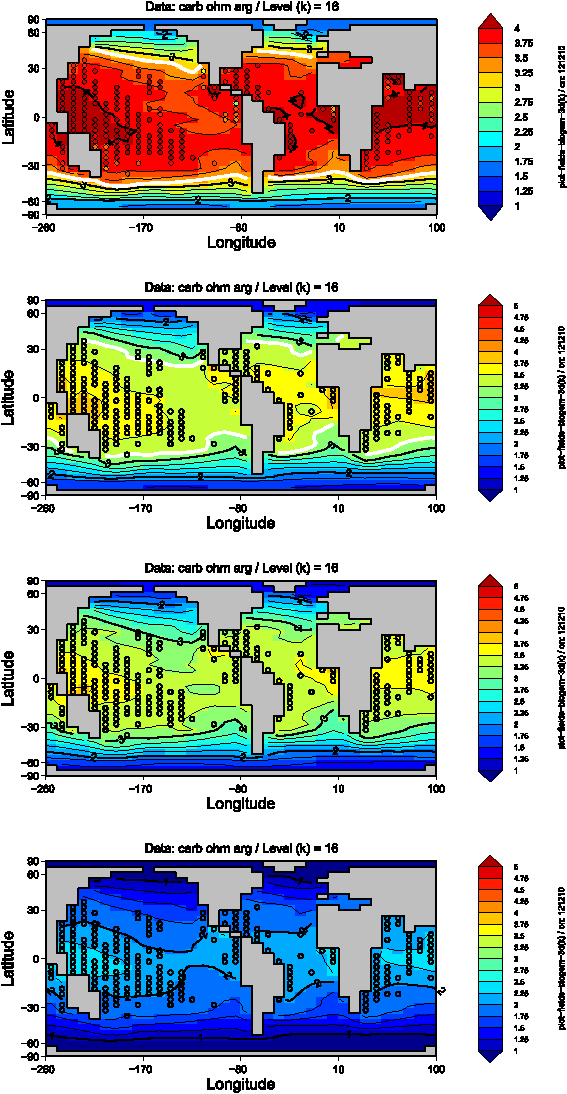
\includegraphics[scale=0.875]{chx-oaimpacts.pdf}
\end{center}
\caption{
\textbf{Mean annual ocean surface saturation (aragonite) changes.}
Top: pre-industrial model ocean surface saturation (aragonite) with ReefBase tropical coral reef locations re-gridded to the \textbf{muffin} grid and color-coded with modern observationally-based saturation values.
2nd and 3rd down: Year 1994 and 2010 ocean surface saturation (aragonite) with ReefBase reef locations.
Bottom: Year 2010 ocean surface saturation (aragonite) under the A2 \(CO_{2}\) emissions scenario.
The thick white line delineates the 3.25 saturation contour (inferred to reflect a limitation on corals).
\textit{Examples here produced using \textbf{muffinplot} but equally do-able in \textbf{Panoply} with the exception of achieving a data overlay. These are provided simply to illustrate some of the impacts you might consider and possible ways of visualizing them.}
}
\label{fig:chx-oaimpacts}
\end{figure}

\begin{figure}[ht]
\begin{center}
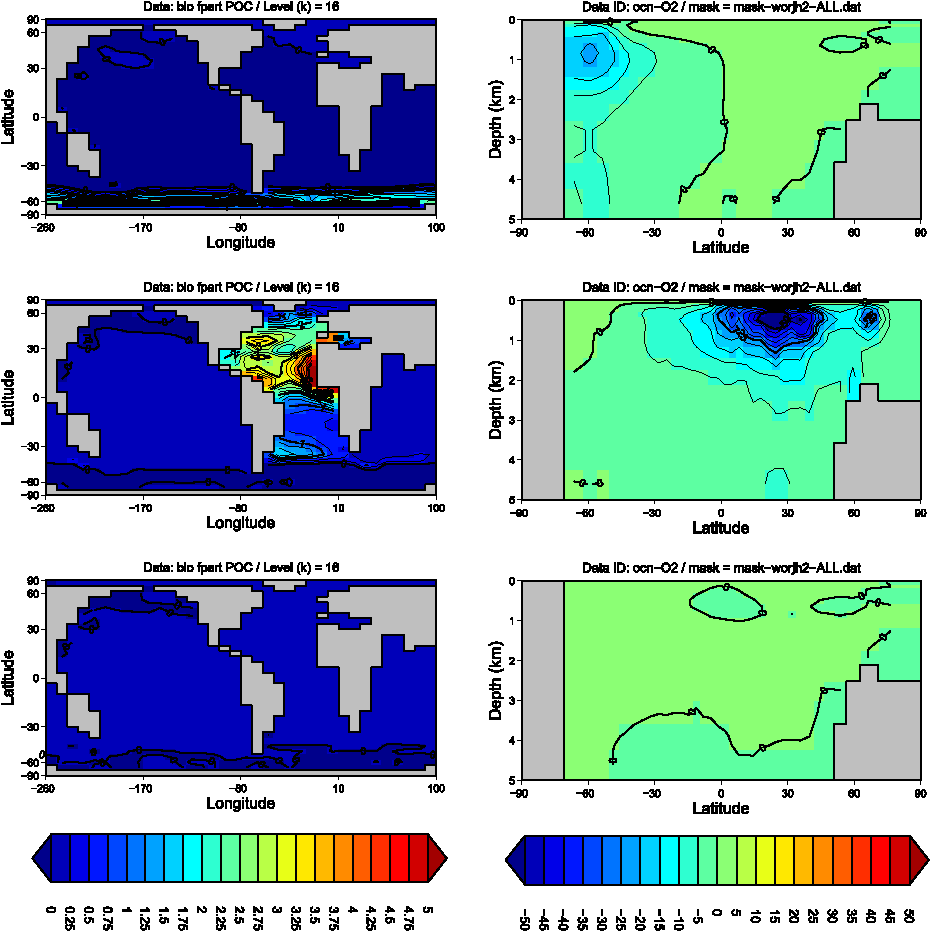
\includegraphics[scale=0.875]{chx-geoengimpacts.pdf}
\end{center}
\caption{
\textbf{Ocean surface export (particulate organic carbon) and zonal \([O_{2}]\) anomalies.}
Left: anomalies of global mean annual export production, for \(Fe\) fertilization (top), \(PO_{4}\) addition (middle), and ocean liming (bottom).
Right: Zonal mean anomalies of dissolved \(O_{2}\) concentrations.
\textit{Examples here produced using \textbf{muffinplot} but equally do-able in \textbf{Panoply} with the exception of achieving a data overlay. These are provided simply to illustrate some of the impacts you might consider and possible ways of visualizing them.}
}
\label{fig:chx-geoengimpacts}
\end{figure}

\newpage 

%------------------------------------------------

\subsection{Further modifications of the biological pump in the ocean}

Other manipulations of the biological pump and ocean carbon cycle are possible and potentially instructive and in the following examples may be of rather more relevance to past climates and carbon cycles and e.g. possible reasons for the low atmospheric \(CO_{2}\) concentrations at the last glacial, as opposed to relevant to geoengineering (a good thing!). The first two of these may have profound effects not only atmospheric p\(CO_{2}\) but also on dissolved oxygen concentrations in the ocean (and hence implications for the suitability of animal habitat such as for fish) and this is something that you will want to look at as part of your overall assessment of impacts.

\subsubsection*{Remineralization depth}

\vspace{2mm}
In the model configuration that you have been using, the degradation of particulate organic matter sinking in the water column proceeds according to a fixed profile of flux with depth (there is no e.g. temperature control on the rate of bacterial degradation of sinking organic matter) with \(CO_{2}\) and \(PO_{4}\) released back to the seawater as the particulate flux decreases. The parameter that controls the (\textit{e}-folding) depth scale of particulate organic matter is:
\vspace{-1mm}\small\begin{verbatim}
bg_par_bio_remin_POC_eL1=589.9451
\end{verbatim}\normalsize\vspace{-1mm}
Either edit this value (found under the heading: \texttt{\# --- REMINERALIZATION ---}) or add a new line at the end of the \textit{user-config} file specifying the value you want. Units are \(m\).

\vspace{1mm}
Read \textit{Ridgwell et al.} [2007] for additional discussion of this parameter. See Figure 2-4 in \textit{Ridgwell} [2001] (http://www.seao2.org/pubs/ridgwell\_thesis.pdf) for an illustration of how the flux of particulate organic matter decreases with depth in the ocean, plus references therein.

There is also an associated parameter: \texttt{bg\_par\_bio\_remin\_POC\_frac2}, which sets a fraction of organic matter that is assumed to settle through the water column completely un-altered (currently assigned a value of 0.045 == 4.5\%), but this is arguably less useful to change than the remineralization length-scale of the more labile fraction (the other 95.5\% of particulate organic carbon exported from the ocean surface).

Note that there may well be no simple parallel that can be found in geoengineering to this process. However, there are hypotheses that during the last glacial and as a result of colder ocean temperatures, the depth scale was longer. Conversely, there are ideas about that the warmer temperatures of the e.g. Eocene ocean and hence faster rates of bacterial metabolism led to a much shallower remineralization depth scale. So a remineralization depth scale that is responsive to temperature may have importance in understanding ocean biogeochemical cycles during both past warm and cold climates as well as obviously, future global change. While you are not implementing a temperature-dependent parameterization explicitly, you can at least test for whether changes in temperature might have important impacts by simply changing the remineralization depth to be shallower (smaller depth-scale under a warming climate) or deeper (greater depth-scale in a colder ocean).

\subsubsection*{Macro nutrient inventory and uptake}

\vspace{2mm}
Suggestions have been made that nutrients were used more efficiently during the LGM, meaning that for the same nutrient uptake at the surface more carbon was exported to depth in the ocean. See: \textit{Omta et al.} [2006]. There are also a bunch of (relatively old) hypotheses concerning differences between glacial and modern ocean in how much nitrate (\(NO^{-}_{3}\)) there was. There is no \(NO^{-}_{3}\) in this version of \textbf{muffin} (just \(PO_{4}\) and \(Fe\)), but an analogous change can be made to the phosphorous cycle.

For the nutrient-to-carbon ratio in organic matter, the relevant parameter is:
\vspace{-1mm}\small\begin{verbatim}
bg_par_bio_red_POP_POC=106.0
\end{verbatim}\normalsize\vspace{-1mm}

\noindent To change the default value (106.0), add a new line at the end of the \textit{user-config} file specifying the value you want. A larger number means that \(PO_{4}\) is being utilized more efficiently and more organic matter is being produced for the same nutrient consumption.

To test the effect of there being more \(PO_{4}\) in the ocean, in addition to using the (surface) flux forcing as described earlier, it is also possible to simply increase the inventory of the ocean as a whole in one go:
\vspace{-1mm}\small\begin{verbatim}
bg_ocn_dinit_8=1.0E-6
\end{verbatim}\normalsize\vspace{-1mm}
which will add \(1\:\mu mol\:kg^{-1}\) of \(PO_{4}\) uniformly to the ocean. (A larger/smaller number will obviously increase the glacial nutrient inventory by more/less.)

In terms of geoengineering, changing the ‘Redfield’ ocean plankton might be difficult … but not impossible, although we are presumably talking about releases of genetically modified organisms to the entire ocean to achieve this meaning there are obviously some severe ethical concerns. However, adding macro nutrients such as \(PO_{4}\) (more often, \(NO^{-}_{3}\) is talked about) may be more feasible.

\subsubsection*{CaCO3:POC rain ratio}

\vspace{2mm}
Kicked off by a classic 1994 \textit{Nature} paper by \textit{Archer and Maier-Reimer} (see: \textit{Kohfeld and Ridgwell} [2009]), one potential means of changing atmospheric \(CO_{2}\) naturally at the last glacial involves changes in the export ratio between \(CaCO_{3}\) (shells) and \(POC\) (particulate organic matter). Such a change in ratio could come about through a variety of ways (e.g., via the 'silica leakage hypothesis' (see: \textit{Kohfeld and Ridgwell} [2009]) and also through the direct effect of \(Fe\) on diatom physiology (see \textit{Watson et al.} [2000] in \textit{Nature} and also Supplemental Information). There are also ideas about an opposite ocean acidification effect, whereby the less acidic glacial (compared to modern) ocean led to increased calcification and \(CaCO_{3}\) export. Note that this response (higher saturation == greater rate of calcification) is encoded into your model configuration – see \textit{Ridgwell et al.} [2007b].

In \textbf{muffin}, the \(CaCO_{3}:POC\) rain ratio is controlled (technically: scaled) by the parameter:
\vspace{-1mm}\small\begin{verbatim}
bg_par_bio_red_POC_CaCO3=0.0485
\end{verbatim}\normalsize\vspace{-1mm}

The pattern of \(CaCO_{3}:POC\) rain ratio is not uniform across the ocean (why? (see: \textit{Ridgwell et al.} [2007, 2009]), and its pattern can be viewed in the (2D \textbf{BIOGEM}) netCDF variable: \textsf{\footnotesize misc\_sur\_rCaCO3toPOC}.

(Note that it is unlikely that there is any parallel in a geoengineering context to this process.)

%----------------------------------------------------------------------------------------
%       CHAPTER X
%----------------------------------------------------------------------------------------

\cleardoublepage

\chapterimage{spore-920.png} % Chapter heading image

\chapter{Marine ecosystems and dynamics}\label{ch:marine-ecosystems}

\hfill \break

\noindent In the chapter we address the role and nature of marine (plankton) ecosystems.\footnote{Loosely based on original workshop material  devised by Ben Ward <b.a.ward@soton.ac.uk>}

\textbf{muffin} includes an explicit ecosystem component, including primary and export production as well as plankton biomass -- \textbf{ECOGEM}\footnote{\href{https://doi.org/10.5194/gmd-2017-258}{\textit{Ward et al.} [2017]} -- Ward, B. A., Wilson, J. D., Death, R. M., Monteiro, F. M., Yool, A., and Ridgwell, A.: EcoGEnIE 0.1: Plankton Ecology in the cGENIE Earth system model, \textit{Geosci. Model Dev. Discuss.}, https://doi.org/10.5194/gmd-2017-258, 2017.} -- as an alternative option to the 'bioloigically induced export flux' representation of export production. The ecological model takes what is known as a size-structured approach to representing diversity of function in marine ecosystems, and is flexible in being able to be configured to represent any range of size classes of phytoplankton and zooplankton (and/or mixotrophs).

\section*{Stuff to keep in mind\dots}
\begin{itemize}
\item We will be working with highly idealised ecosystems in a relatively idealised (modern) ocean.
\item The aim is to explore why the model behaves as it does.
\item The assumption is that this will give us some insight into why the real world behaves as it does. Perhaps. (It is up to you to question the validity of this assumption.)
\end{itemize}

%------------------------------------------------

\newpage

%------------------------------------------------

\section*{Read.me}

\vspace{2mm}
You will need a \textit{re-start} file to carry out the experiments in the Chapter:
\small \begin{verbatim}
$ wget http://www.seao2.info/cgenie_output/wardetal.2018.ECOGEM.SPIN.tar.gz
\end{verbatim} \normalsize

\noindent Extract the results in the usual way and in the usual place ... and return to \textsf{\footnotesize genie-main} in the usual way ... all ... as usual.

%------------------------------------------------

\newpage

%------------------------------------------------

\section{Getting going with ECOGEM}

Previously, you were running the standard 'biogeochemical' version of \textbf{muffin}\footnote{e.g. see \textit{Ridgwell et al.} [2007]}.  In \textbf{BIOGEM}, the biological pump is driven by an implicit (i.e. unresolved) biological community. As in the real ecosystem, the biological uptake of carbon and nutrients (such as phosphorus and iron) is limited by light, temperature and nutrient availability. However, unlike the real ecosystem, any uptake is \textit{directly} and \textit{instantly} converted to particulate and dissolved organic matter (POM, DOM) and exported to the ocean interior via (gravitational) settling and the ocean surface, respectively. i.e.
\vspace{4mm}
\begin{itemize}
\item \underline{surface inorganic nutrients} $\xrightarrow[\rm and~export]{\rm production}$ \underline{POM and DOM}
\end{itemize}
\vspace{4mm}
POM is then instantaneously\footnote{Depending on the specific remineralization options chosen. The default is in fact for POM to settle downwards at a finite rate.} remineralized in the ocean interior, returning nutrients and dissolved carbon and consuming oxygen (amongst other transformations and depending on the specific tracers selected in the ocean). DOM, released in at the ocean surface, is transported with the circulation of the ocean but it fast decay and remineralziation time-scale ensures that nutrients are primarily returned  back to the surface ocean.

In contrast, in this chapter, we are going get started with the '\textbf{ECOGEM}' ecological modeling package. This will allow us to extend the capabilities of \textbf{muffin} to examine a range of questions relating to the role of physiology and community structure in regulating the biological pump and hence atmospheric \(CO_{2}\) etc. In \textbf{ECOGEM}, biological uptake is again limited by light, temperature and nutrient availability, but here it must pass through an explicit and dynamic intermediary plankton biomass pool, before being expressed as the production of POM and DOM (whose fate proceeds as per above):
\vspace{4mm}
\begin{itemize}
\item \underline{surface inorganic nutrients} $\xrightarrow[]{\rm production}$ \underline{plankton biomass} $\xrightarrow[]{\rm export}$ \underline{POM and DOM}
\end{itemize}
\vspace{4mm}

%------------------------------------------------

\subsection{Running the model}

We will start with the simplest possible configuration of \textbf{ECOGEM}, with just a single (small) phytoplankton class\footnote{i.e. as if the ocean was populated with a small species of phytoplankton (photo-autotroph) and nothing else.}. You can run this model at the command line, by entering the following command (note that this should be one continuous line) \dots
\small\begin{verbatim}
$ ./runmuffin.sh muffin.CBE.worlg4.BASESFeTDTL LABS wardetal.2018.ECOGEM.EXAMPLE 10 
     wardetal.2018.ECOGEM.SPIN
\end{verbatim}\normalsize
The model will run as before, except that now we have the \textbf{ECOGEM} debug option enabled, and you will get a lot of extra information about how the ecological model is configured.
\vspace{1mm}

The additional lines appearing as the experiment runs, e.g.
\vspace{-1mm}\small\begin{verbatim}
>>> SAVING ECOGEM TIME-SLICE AVERAGE CENTERED @ year : 0.500
\end{verbatim}\normalsize\vspace{-1mm}
confirm that \textbf{ECOGEM} is writing ecological time-slices at the same time as \textbf{BIOGEM} is writing its own time slices. (Note that \textbf{ECOGEM} is not currently set up to save \textit{time-series} data in the same way as \textbf{BIOGEM}.)

%------------------------------------------------

\subsection{Viewing 2D time-slice output}

Following the same convention as for \textbf{BIOGEM}, \textbf{ECOGEM} \textit{time-slice} output is saved in the subdirectory of your experiment results directory, named \footnotesize\textsf{ECOGEM }\normalsize.\footnote{for this particular example experiment, the full path to the \textbf{ECOGEM} results would be: \\ \scriptsize\textsf{/cgenie\_output/wardetal.2018.ECOGEM.EXAMPLE/ECOGEM/}\normalsize.}

\begin{enumerate}[noitemsep]
\vspace{1mm}
\item Open the \textsf{\footnotesize fields\_ecogem\_2D.nc} file by locating it in the correct directory, and double clicking on it in the file transfer window (if you have that software function configured), or transfer locally and then open (e.g. in \textbf{Panoply}).
\vspace{1mm}
\item You should now see a list of 2D arrays that were output by \textbf{ECOGEM}. Looking at the \textsf{\footnotesize Long Name} description, simply click on a variable of interest. If a menu window pops up, just click on \textsf{\footnotesize Create} or hit the \textsf{\footnotesize Return} key.
\vspace{1mm}
\item Check the \textbf{Panoply} settings to make sure you really know what you are looking at.
\begin{itemize}[noitemsep]
\item Which \textit{time-slice} (i.e. simulation year) are you looking at?
\item What is the data range (i.e. colour scale)
\end{itemize}
\end{enumerate}
\vspace{2mm}

\noindent Remember: you can change the default settings in \textbf{Panoply} to avoid changing things every time you open a new file. First click on \textsf{\footnotesize Panoply} $\rightarrow$ \textsf{\footnotesize Preferences...}. Here you can switch off interpolation and the grid overlay under the \textsf{\footnotesize General} menu. You can disable the spuriously precise coastline under \textsf{\footnotesize Lon-Lat Plots}.

A guide to some key \textbf{ECOGEM} output variables  can be found at the end of Chapter \ref{ch:modeloutput}.

%------------------------------------------------

\subsection{Comparing to observations}

Models are usually intended as an approximation of the real world (whatever that is). It might, therefore, be useful to check if our approximation is in anyway realistic. We can do this by comparing the model output\footnote{NOTE: \textbf{ECOGEM} only saves a limited number of surface (2D) data arrays. You can look at other variables (in 2D and 3D) by opening the corresponding \textbf{BIOGEM} netCDF files.} to observations.

\begin{enumerate}[noitemsep]
\vspace{1mm}
\item You can download a compilation of key biogeochemical variables (as netCDF files) from the \textsf{\footnotesize mymuffin} \href{http://www.seao2.info/cgenie/data/GEnIE_observations.nc}{webpage} ('\textit{Observations for ECOGEM}').
\vspace{1mm}
\item You can open the \textsf{\footnotesize GEnIE\_observations.nc} file in \textbf{Panoply} in the same way as you opened the \textsf{\footnotesize fields\_ecogem\_2D.nc} file.
\vspace{1mm}
\item You can now compare the model output to a variety of key biogeochemical variables that have been derived from ocean measurements. The variables in the \textsf{\footnotesize GEnIE\_observations.nc} netCDf file include:
\begin{itemize}[noitemsep]
\item T and S (not so interesting, except to e.g. evaluate how well \textbf{muffin} simulates different temperature regimes (and habitats)). 
\item DIC and ALK (ignore).
\item Phosphate is of more interest -- how well does \textbf{muffin} simulate surface nutrient availability, and to what degree does ecosystem complexity help explain observations. 
\item Observed Chlorophyll is remote-sensed, and can be contrasted with the chlorophyll biomass simulated by \textbf{ECOGEM}.
\end{itemize}
You might visually compare model with observations, and/or e.g. create difference maps.
\vspace{1mm}
\item When doing this, be asking yourself the question: does the model perform well or poorly with respect to reproducing these variables? If not, \uline{why not}?
\end{enumerate}
\vspace{2mm}

\noindent 

%------------------------------------------------

\newpage

%------------------------------------------------

\section{Ecosystem configuration}

In the last section you ran a very simple configuration of the \textbf{ECOGEM} ecosystem model, and compared it to observations. In this section we are going to add a bit more ecological realism, with the aim of improving model performance (i.e. as contrasted against observations). We will start by adding a zooplankton population that  should bring a degree of `top-down' control to the phytoplankton population.
\vspace{2mm}

Details of the ecosystem are specified in the \textit{user-config} file: \textsf{\footnotesize wardetal.2018.ECOGEM.EXAMPLE}

\begin{enumerate}[noitemsep]
\vspace{1mm}
\item Locate the \textit{user-config} file (in \textsf{\footnotesize \textasciitilde{}/cgenie.muffin/genie-userconfigs/LABS}), and open it in your preferred text editor.
\vspace{1mm}
\item The \textit{user-config} file can be used to configure the ecological model to your liking. 

One of the most important amendments to note straight away can be seen near the very start:
\\\texttt{bg\_par\_bio\_prodopt="NONE"}. This effectively disables the simple biological export scheme in \textbf{BIOGEM}, replacing it with the explicit biology of \textbf{ECOGEM}. This is a necessary step whenever running \textbf{ECOGEM}, because we do not want the implicit and explicit biological schemes to be implemented simultaneously ...
\vspace{1mm}
\item We can also see a load of other model parameters. Any that begin with `\texttt{bg\_}' correspond to \textbf{BIOGEM}, while `\texttt{eg\_}' corresponds to \textbf{ECOGEM}. The \textbf{ECOGEM} parameters begin further down the file.
\vspace{1mm}
\item One of the most important parameters specifies the \textit{ecosystem configuration} file:
\vspace{-1mm}
\small\begin{verbatim}
eg_par_ecogem_plankton_file ='NPD.eco'
\end{verbatim}\normalsize
\vspace{-0mm}
This points to a file (located in \textsf{\footnotesize \textasciitilde{}/cgenie.muffin/genie-ecogem/data/input/}) that specifies every plankton population ('species', if you like) that is accounted for in the model experiment. If you open that file in a text editor, you will see something akin to the following:
\scriptsize\begin{verbatim}
 01                 02    03
 \/                 \/    \/

-START-OF-DATA-
 Phytoplankton    10.00   1
-END-OF-DATA-

 /\                 /\    /\
 01                 02    03

DATA FORMAT AND ORDER
---------------------

COLUMN #01: plankton functional type name
COLUMN #02: plankton diameter (micrometers)
COLUMN #03: number of randomised replicates

INFO: TRACER ASSIGNMENT RULES
-----------------------------
Plankton functional type one of: Prochlorococcus
                                 Synechococcus
                                 Picoeukaryote
                                 Diatom
                                 Coccolithophore
                                 Diazotroph
                                 Phytoplankton
                                 Zooplankton
                                 Mixotroph
\end{verbatim}\normalsize

\newpage

\vspace{1mm}
\item The first thing to note is that only the lines in between the \texttt{\small -START-OF-DATA-} and \texttt{\small -END-OF-DATA-} tags are read by the computer. The rest is there solely for your guidance.

Each line that is entered in the computer-readable area tells the model to create a distinct plankton population in the model. The '`plankton functional type' of this population is specified in the first column, while the plankton diameter is specified in the second column. A `\texttt{1}' must always be placed in the third column (it doesn't 'do' anything, but the model still needs it ...  why ... ?).

In this `NPD' (single nutrient-plankton-detritus) configuration, we only have a 10 micron generic phytoplankton. The ecological and physiological traits of this population are assigned automatically according to the size and the functional type (here: photo-autotroph).

\item[NOTE:] The only PFTs available at the moment are \texttt{Phytoplankton}, \texttt{Zooplankton} and \texttt{Mixotroph}. The other groups currently have no real functionality associated with them.

\item[NOTE:] This file format is fussy, and you\uline{ cannot have any empty lines} in between the  \texttt{\small -START-OF-DATA-} and \texttt{\small -END-OF-DATA-} tags -- every line between these tags must have data (3 parameter values).

\vspace{1mm}
\item We can increase the ecological complexity of the model by adding another plankton population. Save the \textit{ecosystem configuration} file under a new and highly intuitive name (such as \textsf{\footnotesize NP\underline{Z}D.eco}), and add another line specifying a 100 micron zooplankton. It is important that the zooplankton is 10 times larger than the phytoplankton in terms of diameter. This is the optimal predator-prey length ratio in the default configuration. (You could maybe think about changing this value later on.)

\vspace{1mm}
\item  To run the model with this new configuration, change the name of the \textit{ecosystem configuration file} in the \textit{user-config} file\dots
\small\begin{verbatim}
eg_par_ecogem_plankton_file ='NPZD.eco'
\end{verbatim}\normalsize

\vspace{1mm}
\item Save the new \textit{user-config} file under a different name (e.g. \texttt{BSS.NPZD.SPIN}). You can now execute the model at the command line\footnote{Don't forget to change the name of the \textit{user-config} file here as well ...} ...
\small\begin{verbatim}
./muffin.CBE.worlg4.BASESFeTDTL / BSS.NPZD.SPIN 10 wardetal.2018.ECOGEM.SPIN
\end{verbatim}\normalsize
... or submit it to the cluster queue ...
\small\begin{verbatim}
qsub -q dog.q -j y -o cgenie_log -V -S /bin/bash runmuffin.sh
   muffin.CBE.worlg4.BASESFeTDTL / BSS.NPZD.SPIN 10
   wardetal.2018.ECOGEM.SPIN
\end{verbatim}\normalsize

\vspace{1mm}
\item Once you have completed the new simulation, compare the new results to the old simulation, and also in terms of its ability to reproduce observations. Has the addition of zooplankton to the model improved its behaviour or not? Look also at the global distributions of carbon biomass in the phytoplankton and zooplankton populations (again, a log scale might help).

\vspace{1mm}
\textit{How have the zooplankton interacted with the phytoplankton to change the ecological dynamics in the model?}

\end{enumerate}
\vspace{2mm}

%------------------------------------------------

\subsection{Visualising composite data}

We can perhaps get a better handle on this question by looking at the ratio of phytoplankton-to-zooplankton biomass. Such ratios can, however, be difficult to assess simply by eye-balling two maps. Instead we can use \textbf{Panoply} to combine data arrays.

\begin{enumerate}[noitemsep]
\vspace{1mm}
\item First close all your \textbf{Panoply} plot windows. Then open a new one for \textsf{\footnotesize C~Biomass - Popn.~001 (10.00~micron phytoplankton)}. Next, select \textsf{\footnotesize C~Biomass - Popn.~002 (100.00~micron zooplankton)}, and click the \textsf{\footnotesize Combine Plot} icon at the top of the \textbf{Panoply} window.
\vspace{1mm}
\item A box will open up asking you \textsf{\footnotesize In which existing plot should I combine the variable}. As you now only have one plot available, this should be a straightforward choice. Click \textsf{\footnotesize Combine}.
\vspace{1mm}
\item A new map should appear showing the total zooplankton carbon biomass minus the total phytoplankton carbon biomass (see the label on the colour scale). This is not what we want. Below the map, under the \textsf{\footnotesize Array(s)} tab, there is a drop down menu showing the range of different ways the two arrays can be combined. We want to look at the Z:P biomass ratio, so select \textsf{\footnotesize Array 2 / Array 1}.
\vspace{1mm}
\item You now need to make sure that you are looking at the right year (you can time-lock the two arrays by clicking on the chain icon). You may also find it helpful to look at the data on a log scale, with a scale range of \textsf{\footnotesize 0.1} to \textsf{\footnotesize 10}. You might also like to change the \textsf{\footnotesize Color Table:} option to \textsf{\footnotesize GMT\_polar.cpt}.
\end{enumerate}
\vspace{1mm}

Questions:
\vspace{1mm}
\begin{itemize}
\item What does this plot say about the relationship of zooplankton and phytoplankton in different regions of the ocean?
\item In what regions do zooplankton or phytoplankton dominate?
\item What affect does a high Z:P ratio have on the biomass of the phytoplankton population?\footnote{For example, in terms of the chlorophyll concentration.}
\end{itemize}

%------------------------------------------------

\subsection{Iron limitation}

Up to this point, we have only considered phosphate as a limiting nutrient. (Iron was included in the model, but it was not limiting to phytoplankton growth.) You can switch on iron limitation by modifying two lines in the \textit{user-config} file:
\vspace{-2mm}\begin{verbatim}
eg_useFe=.true.
\end{verbatim}\vspace{-2mm}
and
\vspace{-2mm}\begin{verbatim}
eg_fquota=.true.
\end{verbatim}\vspace{-2mm}

Give the \textit{user-config} file a new name (e.g. \texttt{BSS.NPZD\_Fe.SPIN}), then re-run  the model.

\begin{enumerate}[noitemsep]
\vspace{1mm}
\item Examine the effect of iron limitation in the new model. What has changed?

\vspace{1mm}
\item We can get a more exact picture of the nutrient limitation terms via the netCDF output variables: \textsf{\footnotesize eco2D\_xGamma\_Fe\_001} and \textsf{\footnotesize eco2D\_xGamma\_P\_001}.

These two variables take values of between 0 and 1. A \textsf{\footnotesize 1} indicates that the factor is not limiting to growth. A \textsf{\footnotesize 0} indicates the factor is completely preventing growth.
\vspace{1mm}
\begin{itemize}
\item In what regions are iron and phosphorus more or less limiting to growth? \item In regions where neither is limiting, what other factors might be important?
\end{itemize}
\vspace{1mm}

\vspace{1mm}
\item  Plankton stoichiometry plays a critical role in determining which nutrient is most limiting to growth. You can increase the plankton \(Fe:C\) ratio by increasing the minimum and maximum iron quotas. Look at the parameters \texttt{eg\_qminFe\_a} and \texttt{eg\_qmaxFe\_a} in the \textit{user-config} file.

\pagebreak
\begin{itemize}
\item What happens to the ecosystem if you increase these parameters by a factor of 2, 5 or 10?
\item How does a change in these parameters affect the model behaviour?
\item What has changed in terms of the patterns of nutrient limitation?
\item What has happened to the concentration of the limiting and non-limiting nutrient?
\end{itemize}

\vspace{1mm}
\item[NOTE:] It can be 'risky' to just change the parameter value in place, as you might forget what you started with ... Instead; you might copy/paste a new version of the line in question, and comment out the original by placing a `\texttt{\#}' at the beginning of the line. For example:
\vspace{-1mm}\small\begin{verbatim}
#eg_qminFe_a = 3.0e-6
eg_qminFe_a  = 6.0e-6
\end{verbatim}\normalsize\vspace{-1mm}
changes the minimum iron quota by a factor of 2, whilst keeping a record of the original setting (inactivated by the \texttt{\#}). Or, you might do something like:
\vspace{-1mm}\small\begin{verbatim}
eg_qminFe_a  = 6.0e-6 # 3.0e-6
\end{verbatim}\normalsize\vspace{-1mm}
that reduces the total number of lines you end up with in the \textit{user-config} file.

\vspace{1mm}
\item Nutrient supply ratios are also important in determining the limiting nutrient.
\\The \texttt{bg\_par\_det\_Fe\_sol\_exp} parameter determines the solubility of atmospheric iron inputs in seawater. Decreasing the value of \texttt{bg\_par\_det\_Fe\_sol\_exp} will therefore decrease the iron-to-phosphorus supply ratio.

\vspace{1mm}
\begin{itemize}
\item What happens to the ecosystem if you decrease \texttt{bg\_par\_det\_Fe\_sol\_exp} by e.g. 10, 20 or 50\%?
\end{itemize}

\end{enumerate}
\vspace{2mm}

%------------------------------------------------

\newpage

%------------------------------------------------

\section{Increasing ecological complexity}

In the last section, we looked at the results of some simulations based on `NPD' (one nutrient-(phyto)plankton-detritus) and `NPZD' (one nutrient-(phyto)plankton-zooplankton-detritus) type ecosystem models. Here we will begin to incorporate a bit more ecological complexity.

%------------------------------------------------

\subsection{Plankton size classes} We are going to add a few more plankton size classes, so we have small, medium and large phytoplankton and zooplankton.

\begin{enumerate}[noitemsep]
\vspace{1mm}
\item Save the \textit{ecosystem configuration} file under a new name (e.g. \textsf{\footnotesize 3P3Z.eco}), replacing the existing plankton populations with the ones described in Table~\ref{planktonconfig1}.
\vspace{1mm}
\item  To run the model with this new configuration, change the name of the \textit{ecosystem configuration file} in the \textit{user-config} file:
\vspace{-1mm}\begin{verbatim}
eg_par_ecogem_plankton_file='3P3Z.eco'
\end{verbatim}\vspace{-1mm}
\vspace{1mm}
\item Save the new \textit{user-config} file under a different name (e.g. \texttt{BSS.3P3Z.SPIN}) and then run the new model at the command line (e.g. for 10 years).
\end{enumerate}
\vspace{2mm}

\vspace{-4mm}
\begin{table}[htp!]
\begin{center}
\caption{Plankton functional groups and sizes.}
\begin{tabular}{rlc}
\hline
$j$     & PFT                   & \multicolumn{1}{r}{Diameter ($\mu$m)}  \\
\hline
1       & Phytoplankton         & 0.6  \\
2       & Phytoplankton         & 6.0  \\
3       & Phytoplankton         & 60.0  \\
\hline
\end{tabular}
\begin{tabular}{rlc}
\hline
$j$     & Functional Type       & \multicolumn{1}{r}{Diameter ($\mu$m)}  \\
\hline
4       & Zooplankton           & 6.0  \\
5       & Zooplankton           & 60.0  \\
6       & Zooplankton           & 600.0  \\
\hline
\end{tabular}
\label{planktonconfig1}
\end{center}
\end{table}
\vspace{-4mm}

%------------------------------------------------

\subsection{Viewing 2D time-slice output}

Open up the 2D \textit{time-slice} data for the new experiment, following the same procedure as in the previous section. You will now see a lot more \textit{time-slice} variables now appear listed in \textbf{Panoply}. We have all the same diagnostics as before, plus some new ones relating to the new plankton populations you have just added. We also have a load of other arrays describing the size distribution and diversity of the photosynthetic community (non-phototrophic populations are ignored in these metrics). These were not included before, because there was only one phytoplankton population.

\vspace{2mm}
\begin{itemize}[noitemsep]

\item[\textbf{Size fractions}] \
\\Variables beginning ``\textsf{\footnotesize eco2D\_Size\_Frac\_...}'' give the chlorophyll biomass in the three size fractions:
\vspace{1mm}
\begin{enumerate}[noitemsep]
\item picophytoplankton (diameter $\le$ 2 $\mu$m)
\item nanophytoplankton (2 $<$ diameter $\le$ 20 $\mu$m)
\item microphytoplankton (diameter $>$ 20 $\mu$m)
\end{enumerate}
\vspace{1mm}

\item[\textbf{Size metrics}] \
\\Any other variables beginning '\textsf{\footnotesize eco2D\_Size\_...}' give metrics describing the {phytoplankton} size distribution.
\vspace{1mm}
\begin{itemize}[noitemsep]
\item \textsf{\footnotesize eco2D\_Size\_Mean}: Geometric mean\footnote{ We use the geometric mean and standard deviation, because phytoplankton biomass is approximately log-normally distributed across the phytoplankton size range.} phytoplankton diameter, weighted by carbon biomass
\item \textsf{\footnotesize eco2D\_Size\_Stdev}: Geometric standard deviation\footnote{ The geometric standard deviation describes the \textit{relative} size range of the phytoplankton. For a geometric standard deviation of $\sigma$, $\sim$68.2\% of the phytoplankton carbon biomass will be in cells no more than $\sigma$ orders of magnitude smaller or larger than the geometric mean size.} of phytoplankton diameter, weighted by carbon biomass.
\item \textsf{\footnotesize eco2D\_Size\_Minimum}: Diameter of smallest phytoplankton contributing $>$0.1\% of the total phytoplankton carbon biomass.
\item \textsf{\footnotesize eco2D\_Size\_Maximum}: Diameter of largest phytoplankton contributing $>$0.1\% of the total phytoplankton carbon biomass.
\end{itemize}
\vspace{1mm}

\item[\textbf{Diversity metrics}] \
\\Any variables beginning '\textsf{\footnotesize eco2D\_Diversity\_...}' give metrics describing the {phytoplankton} diversity.
\vspace{1mm}
\begin{itemize}[noitemsep]
\item \textsf{\footnotesize eco2D\_Diversity\_Threshold}: the threshold diversity index. The number of species contributing $>$0.1\% of the total phytoplankton carbon biomass [\textit{Barton et al.}, 2010]\footnote{A D Barton, S Dutkiewicz, G Flierl, J Bragg, and M Follows. Patterns of diversity in marine phytoplankton. \textit{Science}, 327(5972):1509–1511, 2010.}.
\item \textsf{\footnotesize eco2D\_Diversity\_Berger}: the inverse Berger(-Parker) index  [\textit{Berger and Parker}, 1970]\footnote{W H Berger and F L Parker. Diversity of planktonic foraminifera in deep-sea sediments. \textit{Science}, 168 (3937):1345–1347, 1970.}. The proportion of carbon biomass made up by all but the single most dominant population. For example, if the dominant population accounts for 40\% of the total carbon biomass, inverse Berger (-Parker) index is 0.6.
\item \textsf{\footnotesize eco2D\_Diversity\_Simpson}: the inverse (Gini-)Simpson index [\textit{Simpson}, 1949]\footnote{E H Simpson. Measurement of diversity. \textit{Nature}, 163:688, 1949.}. This is effectively the probability that two samples taken at random from the community will be from a different species (note that the probability of selecting a population is dependent on carbon biomass, not cell abundance). If we define the proportional biomass of each species as its relative contribution to the total carbon biomass in the community, the inverse Gini(-Simpson) index is calculated as one minus the sum of the squares of the proportional biomasses of each species.
\item \textsf{\footnotesize eco2D\_Diversity\_Shannon}: the Shannon(-Wiener or -Weaver) index  [\textit{Shannon}, 1948]\footnote{C E Shannon. A mathematical theory of communication. \textit{The Bell System Technical Journal}, 27(379-423 and 623-656), 1948.}. With the proportional biomass defined as above, the Shannon index is defined as the sum of [the proportional biomass multiplied by the logarithm of the proportional biomass] for each species.
\item[NOTE:]The threshold index is a fairly crude measure of the total number of species in the community, relative to a small and arbitrary threshold of relative biomass. This index is not very sensitive to the relative biomass of individual species (although one very successful species can raise the absolute value of the threshold, thus lowering the diversity).
\\The other three indices do more to quantify the evenness of the community. The more unequal the proportional abundances, the smaller the value of the index. If almost all the abundance is concentrated into one type and all the other types are very rare, the latter three indices can become very small. A community with fewer species, but with more evenly distributed biomass, may well have higher values for these three diversity indices.
\end{itemize}
\vspace{1mm}

\end{itemize}
\vspace{1mm}

\pagebreak

Have a look at some of these metrics, but bear in mind that they summarise the diversity of a phytoplankton community that includes just three species. They are probably not that revealing, so we will come back to them later. Instead, have a look some of the other metrics describing the model ecosystem.

\vspace{1mm}
Questions:
\vspace{1mm}
\begin{itemize}
\item What are the global distributions of the different size classes?
\item How do the global biomass distributions compare to variables such as temperature\footnote{Ocean temperature is saved in \textsf{\scriptsize fields\_biogem\_3D.nc}}, or primary production (\textsf{\footnotesize Uptake Fluxes C})?
\item How does nutrient, light and temperature limitation vary between the size classes?
\item Can you account for the distribution biomass between the size classes according to the different limiting factors?
\end{itemize}
\vspace{2mm}

%------------------------------------------------

\subsection{Create your own ecosystem}

Save the \textit{ecosystem configuration} file under a new name and add some more plankton populations (whatever and as many as you like\footnote{Just bear in mind that the more populations you put in, the slower the model will run!}). Update the \textbf{muffin} parameter \texttt{eg\_par\_ecogem\_plankton\_file} in the \textit{user-config} and save this file under a new name.  Run the new model.

\vspace{1mm}
Questions:
\vspace{1mm}
\begin{itemize}
\item How many populations can you get to coexist (i.e. each having a non trivial ($>$0.1\%) biomass)?
\item What effect do the new populations have on the community as a whole?
\item What effect, if any, do your additions have on the strength of biological export?\\(e.g. look at \textsf{\footnotesize bio\_fpart\_POC} in \textsf{\footnotesize fields\_biogem\_3D.nc}.)
\end{itemize}
\vspace{2mm}

%------------------------------------------------

\newpage

%------------------------------------------------

\section{Build it up, tear it down}

%------------------------------------------------

\subsection{A fully size-structured  ecosystem} We are now going to switch to a more diverse version of the size-structured ecosystem model. This configuration has 8 size classes of phytoplankton, and 8 size classes of zooplankton, as shown in Table~\ref{planktonconfig2}.

\begin{enumerate}[noitemsep]
\vspace{1mm}
\item Save the \textit{ecosystem configuration} file under a new name, replacing the existing plankton populations with the ones described in Table~\ref{planktonconfig2}.
\vspace{1mm}
\item Update the \textit{user-config} to point to the new \textit{ecosystem configuration} file, and save again under a new name. (It is generally a good idea to make a note of the name and goal of each experiment as you set it up.)
\vspace{1mm}
\item Run the new model for at least 20 years (this will probably take about 10-15 minutes).
\end{enumerate}
\vspace{2mm}

\begin{table}[htp!]
\begin{center}
\caption{Plankton functional groups and sizes.}
\begin{tabular}{rlc}
\hline
$j$     & PFT                   & \multicolumn{1}{r}{Diameter ($\mu$m)}  \\
\hline
1       & Phytoplankton         & 0.2  \\
2       & Phytoplankton         & 0.6  \\
3       & Phytoplankton         & 1.9  \\
4       & Phytoplankton         & 6.0  \\
5       & Phytoplankton         & 19. 0 \\
6       & Phytoplankton         & 60.0  \\
7       & Phytoplankton         & 190.0  \\
8       & Phytoplankton         & 600.0  \\
\hline
\end{tabular}
\begin{tabular}{rlc}
\hline
$j$     & Functional Type       & \multicolumn{1}{r}{Diameter ($\mu$m)}  \\
\hline
9       & Zooplankton           & 0.6  \\
10      & Zooplankton           & 1.9  \\
11      & Zooplankton           & 6.0  \\
12      & Zooplankton           & 19.0 \\
13      & Zooplankton           & 60.0  \\
14      & Zooplankton           & 190.0  \\
15      & Zooplankton           & 600.0  \\
16      & Zooplankton           & 1900.0  \\
\hline
\end{tabular}
\label{planktonconfig2}
\end{center}
\end{table}
\vspace{-4mm}

%------------------------------------------------

\subsection{Ecosystem characteristics} We can now begin to look at the size and diversity metrics of the phytoplankton community in a meaningful way.

\begin{enumerate}[noitemsep]
\vspace{1mm}
\item Look first at:
\begin{enumerate}[noitemsep]
\item the total carbon biomass
\item the carbon uptake flux (i.e. primary production)
\item the geometric mean size
\end{enumerate}
Make sure in each case that you are looking at the last year of model output. You may also find it useful to adjust the colour scale, or to change to a logarithmic colour scale (e.g. try a logarithmic scale from 2 to 20 microns for the geometric mean size).
\\Looking at the maps, we can perhaps pick out three different ``biomes'' in terms of their community properties:
\begin{enumerate}
\item The low-latitude oligotrophic gyres are relatively unproductive, and support some of the lowest annual mean biomass in the surface ocean. In these regions the mean phytoplankton size is very small.
\item Subpolar latitudes between 40$^\circ$ and 50$^\circ$ (either N or S) are much more productive, and support very high annual mean biomass. These communities also have the highest mean sizes of any region.
\item The polar oceans are also highly productive (except perhaps the high Arctic), and support relatively high annual mean biomass. These communities are made up (in the model, at least) of slightly smaller phytoplankton than we see in the subpolar regions.
\end{enumerate}
\vspace{1mm}
\item What can we find out about the community structure in these regions? Open up some of the other metrics describing the community (standard deviation of size distribution, size fractionation, diversity, limiting factors). What can you find out about the community structure within each region, in terms of coexistence and exclusion?
\vspace{1mm}
\begin{itemize}
\item Does the community span a broad or narrow size range?
\item How many size classes are coexisting in each biome?
\item What is the smallest and largest size class in each biome?
\item How much biomass is concentrated in each size fraction (picoplankton, nanoplankton and microplankton)?
\end{itemize}
\end{enumerate}
\vspace{1mm}

Overall -- what factors do you think are most important in terms of dictating the global distribution of each size class?

To find out the answers to these questions, you are going to pull the model apart, and then put it back together. At each stage the aim is to bring in a different limiting factor, so that you can see its effect on the model behaviour.

%------------------------------------------------

\subsubsection*{The fundamental niche}

The first step is to find out the impact of abiotic factors on the distribution of different phytoplankton sizes. In other words, we need to find out what the distribution of the phytoplankton would be in the absence of any ecological interactions, such as resource competition and predation. This is effectively their `fundamental niche'.

The fundamental niche is fairly abstract, and not something that can be measured in the real world. In model world, however, we can get a useful estimate of the fundamental niche by making a few simple changes to the model.

\begin{enumerate}[noitemsep]
\vspace{1mm}
\item First of all, you can remove all predation, simply by removing the zooplankton from the \textit{ecosystem configuration} file. Once again, you will need to save a new and appropriately named \textit{user-config} file.
\vspace{1mm}
\item Next, you also need to remove all competition for nutrients and light. This involves tweaking the model equations so that the phytoplankton are not nutrient limited, and do not attenuate light. To do this, all you need is to add the following line to the \textit{user-config} file.
\vspace{-1mm}
\small\begin{verbatim}
eg_fundamental = .TRUE.
\end{verbatim}\normalsize
\vspace{-1mm}
\item If you now run the model (just 10 years should do it, in this case), you should have a community of eight phytoplankton size classes that are growing solely as a function of the incoming light and the temperature. This growth will be balanced balanced the basal (i.e. non-grazing) mortality. As there is no feedback between the ecosystem and the environment, populations that can survive will grow exponentially and without limit, potentially reaching astronomical abundance in very little time. Populations that cannot survive will rapidly decline to almost nothing.
\\The regions in which each plankton shows positive growth defines its fundamental niche. This is a function of abiotic conditions only, and is the absolute limit of its geographical range. Look at the carbon biomass distribution in each size class (set the data range in each case from \(0\) to \(1mmolCm^{-3}\)).
\vspace{1mm}
\begin{itemize}
\item How and why does the fundamental niche vary with size?
\item Could the limits of the fundamental niche explain some of the patterns seen in the full model?
\end{itemize}

\end{enumerate}
\vspace{2mm}

%------------------------------------------------

\subsubsection*{Resource competition.}

The next step is asses the impact of resource competition. We are first going to do this in the absence of any zooplankton grazing.

\begin{enumerate}[noitemsep]
\vspace{1mm}
\item All you need to do at this stage is to re-enable nutrient and light competition. To do this, simply delete `\texttt{eg\_fundamental~=~.TRUE.}' from the \textit{user-config} file (or comment out the line to disable it), and save under a new name. Leave the \textit{ecosystem configuration} file as it is.

\vspace{1mm}
\item You should have a community of eight phytoplankton size classes that are competing for nutrients and light, again as a function of temperature. This is a much more realistic simulation, as feedbacks between the ecosystem and the environment serve to limit the size of the phytoplankton populations. Examine the model to find out:
\vspace{1mm}
\begin{itemize}
\item What size classes are able to persist when resource competition is enabled?
\item Why are different size classes more or less abundant in different areas?
\item How does the distribution of each size class compare to the fundamental niche?
\item What are the reasons for any differences?
\end{itemize}
\end{enumerate}
\vspace{1mm}

Phytoplankton biogeography at this stage begins to approximate the realised niche, which defines the range of conditions that support a population in the presence of ecological interactions. Note that at this stage, however, we have ignored the effects of any predator-prey interactions, as the zooplankton grazers are still missing.

%------------------------------------------------

\subsubsection*{Resource competition + one generalist zooplankton}

The previous simulation is clearly unrealistic (although, hopefully, informative). You are now going to add back in just a single zooplankton class, that grazes equally on all plankton (including itself).

\begin{enumerate}[noitemsep]
\vspace{1mm}
\item Add a 100 micron zooplankton into the \textit{ecosystem configuration} file, and save under a new name. Also update the \textit{user-config} file to reflect the change, and save under a similar name.
\vspace{1mm}
\item You need to modify the model so that the zooplankton eats all prey with equal preference. This can be done by adding the following lines to the \textit{ecosystem configuration} file.
\vspace{-1mm}\small\begin{verbatim}
eg_ns=1
eg_pp_sig_a=1.0e99
\end{verbatim}\normalsize\vspace{-1mm}
\item[NOTE:] For aficionados, the first parameter disables prey-switching (i.e. predators no longer preferentially attack the most abundant prey). The second parameter increases the width of the grazing kernel (i.e. predators can attack a range of prey across a huge size range with equal preference).
\vspace{1mm}
\item The addition of zooplankton to the model community should give a more accurate approximation of the realised niche.
\vspace{1mm}
\begin{itemize}
\item Does the addition of a single zooplankton grazer enable more or less coexistence?
\item What factors might be responsible for any shifts in biogeography?
\end{itemize}
\end{enumerate}

%------------------------------------------------

\subsubsection*{Resource competition + one ``switching'' zooplankton}

You began with a full food-web containing 8 phytoplankton and 8 zooplankton size classes. The diversity of zooplankton clearly has an effect on the phytoplankton community that is not seen in the previous experiment. This effect can be imitated with just one generalist zooplankton if we instruct it to graze preferentially on the most successful prey.

\vspace{8mm}
\pagebreak

Re-enable this 'prey switching' effect by changing the following control parameter to a \texttt{2}:
\vspace{-1mm}\small\begin{verbatim}
eg_ns=2
eg_pp_sig_a=1.0e99
\end{verbatim}\normalsize\vspace{-1mm}
Compare this simulation to the first experiment (8 phytoplankton and 8 zooplankton) to see how the inclusion of prey switching increases coexistence through the `kill-the-winner' mechanism.

\vspace{1mm}
\begin{itemize}
\item How does nutrient limitation change with phytoplankton size, and how might zooplankton be affecting this?
\item Look at the C:P biomass ratio in the community as a whole, and compare to your estimates from the NPZD model (Lesson~1).
\item How does the C:P ratio vary with size? How does having a diverse community affect the coupling of carbon and limiting nutrients?
\end{itemize}

%------------------------------------------------

\subsection*{Further questions to answer}

\begin{itemize}
\item What sets the fundamental niche, and how does it change with size?
\item How is the fundamental niche modified by resource competition?
\item What species are favoured in terms of nutrient competition?
\item How is the outcome of competition affected by...
\begin{itemize}
\item Abiotic conditions?
\item Increased mortality (through generalist grazing)?
\item Density-dependent mortality (through specialist grazing)?
\end{itemize}
\item Do these experiments tell you all you need to know?\\What other modifications can you think of making?
\end{itemize}

%------------------------------------------------

\subsection{Mixotrophy}

Try adding some mixotrophs to the phytoplankton and zooplankton already present in the community. These will have exactly half the nutrient uptake traits of phytoplankton of a similar size, and half the prey capture traits of zooplankton if a similar size. To do this:

\begin{enumerate}[noitemsep]
\vspace{1mm}
\item Save the previous \textit{ecosystem configuration} file under a new name.
\vspace{1mm}
\item Edit the new \textit{ecosystem configuration} file and add an additional line to add a mixotroph:
\vspace{-1mm}\begin{verbatim}
 Mixotroph    xxx   1
\end{verbatim}\vspace{-1mm}
where \texttt{xxx} is the class size of the mixotroph. (And remember to save it.)
\vspace{1mm}
\item Update the \textit{user-config} to point to the new \textit{ecosystem configuration} file, and save again under a new name. (It is generally a good idea to make a note of the name and goal of each experiment as you set it up.)
\vspace{1mm}
\item Run the new model for at least 10-20 years.
\end{enumerate}
\vspace{1mm}

\noindent Further questions to explore/answer:

\vspace{1mm}
\begin{itemize}
\item How does this effect the mean and standard deviation of cell size?\\(Size and diversity metrics will be calculated for phytoplankton and mixotrophs together)
\item How does mixotrophy effect the C:P ratio of organic matter?
\item How does the realised niches of mixotrophs compare to the fundamental niches of phytoplankton?
\end{itemize}

Also: try replacing all the phytoplankton and zooplankton with a range of sizes of mixotrophs. How does the simulation differ from one with the same size range of sperate phytoplankton and zooplankton classes?

For instance -- you might also try having an ecosystem comprising just a single small (e.g. \(10 \mu m\) mixotroph (no phytoplankton and no zooplankton), and perhaps an ecosystem with one small mixotroph \(10 \mu m\) and one additional mixotroph, 10 times lager \(100 \mu m\). Compare the productivity of such an ocean compared to some of your previous simplified ecosystem configurations (such as a single small \(10 \mu m\) phytoplankton, and a configuration with a single small phytoplankton and a single larger \(100 \mu m\) grazer).
%
%------------------------------------------------

\newpage

%------------------------------------------------

\section{Ecology in ... future oceans}

What might happen to primary production and the biological pump as (future) climate continues to change? What might happen to the distribution of species (here: size classes) in the ocean? Does it 'matter' (e.g. for marine bio geochemical cycling and feedbacks on atmospheric \(pCO_{2}\)? (And how different is the Earth system response when using a complex ecosystem model rather than the highly simplified representation of biological export you used previously?)

\vspace{1mm}
There are all good questions for a model!

\vspace{1mm}
The best place to start is with the full complexity ecosystem structure with 8 size classes for both phytoplankton and zooplankton (as described in \textit{Ward et al.} [2018]), and continuing on from a \textit{re-start} of the pre-industrial ocean (and ecology) -- \texttt{wardetal.2018.ECOGEM.SPIN}. 

For the \textit{user-config} -- for which you can either adapt your own based on your earlier ecosystem experimenting, or adapt the published configuration used to create the \textit{re-start} -- \\\texttt{wardetal.2018.ECOGEM.SPIN} (in: \textsf{\footnotesize user-configs/MS/wardetal.2018}) -- \uline{NOTE the different \textit{user-config} directory}!!! and \uline{remember to rename it}\footnote{The new \textit{user-config} file need not be sabed back into this same directory.} so you do not overwrite the \textit{re-start} ... \footnote{The \textit{base-config} is as per you have been using in this Chapter -- \texttt{muffin.CBE.worlg4.BASESFeTDTL}} 
\vspace{2mm}

Then:

\begin{enumerate}[noitemsep]

\vspace{1mm}
\item First, create a \textit{control}, e.g. based on \texttt{wardetal.2018.ECOGEM.SPIN}, so that you can more easily spot any mis-matched parameter values or other problems -- do to this, turn off the atmospheric \(pCO_{2}\) \textit{forcing} (so that \(pCO_{2}\) can respond to and indicate any significant changes in the marine carbon cycle), but leave on the dust flux \textit{forcing} (because we still need a supply of dissolved iron to the ocean surface):
\vspace{-1mm}\small\begin{verbatim}
# specify forcings
bg_par_forcing_name="worlg4.FeMahowald2006"
\end{verbatim}\normalsize\vspace{-1mm}

\vspace{1mm}
\item Second, you will need either:

\vspace{1mm}
\begin{itemize}[noitemsep]
\item A \textit{user-config} with an conceptual emissions scenario (e.g. anything that you have played with previously). This can be run directly on from the pre-industrial spin-up.

This will allow you to explore questions concerning the impact on marine ecosystems and carbon cycling of the rate of warming (driven by your assumed rate of carbon emissions), and/or the importance of and sensitivity of marine ecosystems and carbon cycling, to the total (maximum) warming.

\vspace{1mm}
A template emissions \textit{forcing} (plus dust) is provided as:
\vspace{1mm}
\\\textsf{\footnotesize worlg4.FpCO2\_Fp13CO2.FeMahowald2006}

\vspace{1mm}
As per before, you need to re-scale the values in the forcing because the \(CO_{2}\) flux is assumed to be in units of \(PgC\:yr^{-1}\) \footnote{As per notes in the \textit{forcing} \textit{time-series} \textsf{\footnotesize .sig} file itself.} (and \(\delta^{13}C\) is given a default value of \(1.0\)). i.e. add the lines:
\vspace{-1mm}\small\begin{verbatim}
bg_par_atm_force_scale_val_3=8.3333e+013
bg_par_atm_force_scale_val_4=-27.0
\end{verbatim}\normalsize\vspace{-1mm}
and remember that the forcing is provided as a pulse of \(1\:molyr^{-1}\) (\(1PgC \:yr^{-1}\) when scaled) carbon emissions over just a single year, and hence the \textit{time-series} file for the \textit{forcing}: \textsf{\footnotesize biogem\_force\_flux\_atm\_pCO2\_sig.dat} needs to be edited -- see Chapter \ref{ch:fossil-fuel-co2}.

\end{itemize}

\newpage
Or:

\begin{itemize}[noitemsep]
\item A historical transient (plus dust) \textit{forcing} and then run from e.g. 1750 through 2010 (as per before), for which the forcing is:
\vspace{1mm}
\\\textsf{\footnotesize worlg4.historical2010.FeMahowald2006}

\vspace{1mm}

\vspace{1mm}
Remember that here that you do not re-scale the atmospheric \(pCO_{2}\) (or \(\delta^{13}C\)) value as was done with the forcing used to generate the re-start (this historical transient forcing includes the actual values of  \(pCO_{2}\) and in the correct units). 

\vspace{1mm}
Note that with the full complexity ecosystem model included, the 245 years of this experiment will take much longer than before when you ran a historical transient experiment. You could 'cheat' a little and start from year 1850 rather than 1765, on the basis that nothing much happens in between (in terms of rising \(pCO_{2}\) and warming). To do this -- simply run the transient experiment only for 160 years (1850 to 2010) and adjust the starting date in the \textit{user-config}:
\vspace{-1mm}\small\begin{verbatim}
# change start year
bg_par_misc_t_start=1850.0
\end{verbatim}\normalsize\vspace{-1mm}

\vspace{1mm}
You will also need \textit{time-series} and \textit{time-slice} saving that aligns with the historical (and future) period:
\vspace{-1mm}\small\begin{verbatim}
# save frequency
bg_par_infile_slice_name='save_timeslice_historicalfuture.dat'
bg_par_infile_sig_name='save_timeseries_historicalfuture.dat'
\end{verbatim}\normalsize\vspace{-1mm}
(i.e. just as before when you ran a historical transient).

Once you have run this experiment, you can use it as a \textit{re-start} for a future emissions scenario,  with a \textit{forcing} adapted from e.g. \textsf{\footnotesize worlg4.FpCO2\_Fp13CO2.FeMahowald2006} and remember to add the emissions units scaling:
\vspace{-1mm}\small\begin{verbatim}
bg_par_atm_force_scale_val_3=8.3333e+013
bg_par_atm_force_scale_val_4=-27.0
\end{verbatim}\normalsize\vspace{-1mm}

\end{itemize}

\vspace{1mm}
\noindent Whichever route you chose, will also require (another) control experiment run for the same number of years (and with dust but not \(pCO_{2}\) \textit{forcing}).

\end{enumerate}

\vspace{1mm}
\noindent What to look for? The questions (at the start) should help guide you in this, and might include:

\vspace{1mm}
\begin{itemize}[noitemsep]
\item Patterns of primary productivity and export (where do they increase, decrease), plus time-series of global totals (what is the global impact of warming?).
\item Patterns of ocean oxygenation (and patterns of dysoxia and anoxia).
\item Surface ocean nutrient distributions, and nutrient limitation.
\item Spatial patterns of plankton size -- either simply for mean size, or look at the patterns of biomass of specific size classes. (You might follow a the preferred habitat/location of a particular size class with latitude to see whether it experiences a 'range shift'.)
\item Diversity etc.
\end{itemize}

\vspace{1mm}
\noindent You might also contrast with emissions scenarios that you might have run previously employing the simplified biological export scheme in \textbf{BIOGEM}, rather than the complex ecosystem model of \textbf{ECOGEM}. (Make sure you are comparing between the same emissions scenarios). The question to be answered would be: does representing marine ecology 'matter'?

%------------------------------------------------

\newpage

%------------------------------------------------

\section{Ecology in ... past oceans}

Here we consider a series of examples\footnote{Either published or in the works or existing in some publication fantasy ...} of the \textbf{ECOGEM} model of marine ecology, applied to published paleo configuration of \textbf{muffin} and used to ask questions of how different could marine carbon cycling (and atmospheric \(pCO_{2}\)) and oxygenation have been in the (relatively recent) past and how do model projections compare with proxy observations.

The three examples come firstly from the Last Glacial Maximum, with direct comparison being made to post glacial time (here, the late Holocene), with the intention to explore the role of climate cooling, altered ocean circulation, and increased iron supply to the ocean in modifying plankton distributions and size structures. Secondly, from around the time of the Paleocene-Eocene Thermal Maximum (PETM) some 55 Myr ago, now both considering a different paleogeography, a warmer ocean, and then transient warming on top of that. Lastly we turn to marine ecology and carbon cycling in the aftermath of the impact and extinction event at the end of the Cretaceous, some 66 Myr ago, and return to our earlier exploration of what happens if you lose the larger plankton in the ocean.

%------------------------------------------------
\newpage
\subsection*{The Last Glacial}

The Last Glacial Maximum (LGM) (ca. 19 to 23 ka) was characterized by lower sealevel and higher ocean salinity, colder ocean temperatures, and a reorganized meridional overturning circulation in the Atlantic. The latter 2 changes in particular should have impacted marine ecosystems and indeed, observations suggest range migration (temperature-tracking) and shifts in the zone of highest productivity in the Southern Ocean, amongst other impacts. The aim of this particular investigation, is to assess what these ecological changes are (at least in model world).

Provided is a configuration of LGM ocean circulation that has been tuned to fit observations of benthic carbon isotopes, which provide an observational constrain on large-scale ocean circulation. To this, you'll an ecosystem (in place of the default \textbf{BIOGEM} 'induced export' scheme). Also provided is a \textbf{muffin} configuration for late Holocene ('HOL') (0-6 ka), created in exactly the same way and also tuned to respective (0-6 ka) benthic carbon isotope data. Configuration HOL provides a point of comparison (or control) for you to compare the ecology in a colder, LGM ocean against.\footnote{i.e. you run pairs of HOL and LGM experiments and contrast between them, rather than necessarily comparing to previous modern configurations.}

\vspace{1mm}

The \textit{user-configs} you need to use, or copy-rename, can be found in the directory:
\vspace{1mm}
\\\textsf{\footnotesize genie-userconfigs/MS/odalenetal.CP.2019}
\vspace{1mm}
\\\noindent(and you can run your experiments from here\footnote{If you use them in this directory, make sure at the command line, you replace LABS with \texttt{MS/odalenetal.CP.2019}.}, or better, copy-edit-rename the \textit{user-configs} you run experiments with, from the \textsf{\footnotesize LABS} sub-directory).

Read the \textsf{\footnotesize readme.txt} file for instructions for the basic set of command line parameters needed, but remember that you may be running your \textit{user-config} with a different name and likely from a different sub-directory.
Spin up the following experiments  (and then experiment with them later)\footnote{Noting that the long file-names differ only in a single '\textsf{v}' vs. an '\textsf{a}' ...}:

\vspace{1mm}
\begin{itemize}[noitemsep]
\item[(1)] \textsf{\footnotesize muffin.CB.GIteiiaa.BASESFeTDTL\_rb } \textit{base-config} \\+ \textsf{\footnotesize muffin.CB.GIteiiaa.BASESFeTDTL\_rb.SPIN } \textit{user-config}
\item[(2)] \textsf{\footnotesize muffin.CB.GIteiiva.BASESFeTDTL\_rb } \textit{base-config} \\+ \textsf{\footnotesize muffin.CB.GIteiiva.BASESFeTDTL\_rb.SPIN } \textit{user-config}
\end{itemize}
\vspace{1mm}

\noindent Submit these to the cluster ...  remembering that you will need to recompile \textbf{muffin} between (1) and (2) (and potentially also re-compile before running (1) if you have not  used that particular \textit{base-config} immediately prior). Run the spin-ups for 10,000 years.

Neither of these configurations currently have an ecosystem enabled, but they will provide a baseline against which you can  contrast a pair of experiment that include explicit ecology. What you need to do know is to add in/enable \textbf{ECOGEM}. To do this, you need to modify both \textit{base-} and \textit{user-config} files of both the HOL and LGM model configurations.\footnote{Strongly recommended that that you copy-rename both sets of files and edit the copies.}

\begin{enumerate}[noitemsep]

\vspace{1mm}
\item \textit{base-config} -- First, you need to enable the \textbf{ECOGEM} module.
\\At the top of the HOL \textit{base-config} file \textsf{\footnotesize muffin.CB.GIteiiaa.BASESFeTDTL\_Crb}\footnote{And similarly for the LGM one.} you will see the line:
\vspace{-2mm}\begin{verbatim}
ma_flag_ecogem=.FALSE.
\end{verbatim}\vspace{-2mm}
Simply change this to \texttt{.TRUE.}
\vspace{6mm}
\pagebreak

\vspace{1mm}
\item \textit{user-config} -- Next, some deletions and additions are needed in the \textit{user-config} provided (which only has implicit biological export enabled).
\\In the section of the file under the heading:
\footnotesize\begin{verbatim}
#
# --- BIOLOGICAL NEW PRODUCTION -------------------------------------
#
\end{verbatim}\normalsize
you are going to delete everything there (in that section) and replace it with:
\vspace{-1mm}\begin{verbatim}
# biological scheme ID string
bg_par_bio_prodopt="NONE"
\end{verbatim}\vspace{-1mm}
The only other thing you need then is a section of code that defines all the \textbf{ECOGEM} ecological parameters.
\\ Go open file \textsf{\footnotesize wardetal.2018.ECOGEM.SPIN}, which you can find in the \textit{user-config} sub-directory \textsf{\footnotesize MS/wardetal.2018}, and you'll see under the heading:
\footnotesize\begin{verbatim}
#
# --- ECOGEM ----------------------------------------------------------
#
\end{verbatim}\normalsize
a long list of parameter settings (down to the next section headed \texttt{DATA SAVING}). Simply copy-paste this entire section (including \texttt{ECOGEM} header lines if you like), anywhere in your \textit{user-config} file. At the very end of the file would do just fine.\footnote{Try and ensure that there is blank line at the very end of the file just in case \textbf{muffin} has any problems reading it in.}

And lastly ... under:
\footnotesize\begin{verbatim}
#
# --- MISC ----------------------------------------------------------
#
\end{verbatim}\normalsize

(and the end of the section) add the following lines
\vspace{-1mm}\begin{verbatim}
# kraus-turner mixed layer scheme on (1) or off (0)
go_imld = 1
\end{verbatim}\vspace{-1mm}
This enables a 'mixed layer depth' scheme in the ocean circulation model that \textbf{ECOGEM} needs to calculate light limitation during esp. intervals of high latitude / wintertime deep mixing.

This ... should do-it, i.e. you have added the same tuned ecosystem model as described in \textit{Ward et al.} [2018] to your LGM / HOL \textit{user-configs}.

\end{enumerate}

\vspace{1mm}

Now you are ready to run new LGM and HOL experiments, with a full ecosystem in each\footnote{Remembering that presumably both your \textit{base-config} and \textit{user-config} file names are  different as compared to running the non \textbf{ECOGEM} version described in the \textsf{\footnotesize readme}.}.
\vspace{1mm}

Obvious questions to investigate include not only how ecosystems and patterns of biological export may have differed between LGM and HOL, but also how patterns of nutrients (\(PO_{4}\) and \(Fe\)) may have differed ... and also distributions of dissolved \(O_{2}\) in the ocean (and in the interior, rather than across the ocean surface). A water mass ventilation age tracer has also been simulated and the results of this will help in understanding how global circulation patterns differ between the 2 time intervals.

You can also compare between with and without \textbf{ECOGEM} versions as the only thing that changes between pairs of HOL or pairs of LGM experiments is the biological scheme\footnote{Actually, this is not true, as in the \textbf{ECOGEM} enabled experiments, the mixed layer scheme in the coean circulation model is also activated and which has an impact on ocean circulation. You could then create a 3rd set of HOL+LGM experiments, using the basic \textbf{BIOGEM} implicit export biological scheme, but now also setting the \texttt{go\_imld} parameter to a value of \texttt{1}}.

%------------------------------------------------
\newpage
\subsection*{The PETM}

In this practical we are going to look at the ocean as it \textit{might} have been just over 55 million years ago, at the Paleocene-Eocene Thermal Maximum (PETM) -- in short a lot warmer, and with a somewhat different continental configuration and hence ocean circulation. The exercise is based on a recent 'ECOGENIE' (\textbf{muffin} configured to include \textbf{ECOGEM}) publication\footnote{Wilson, J.D., F.M. Monteiro, D.N. Schmidt, B.A. Ward, and A. Ridgwell, Linking marine plankton ecosystems and climate: A new modeling approach to the warm early Eocene climate, Paleoceanography and Paleoclimatology, 33, 1439–1452, DOI: 10.1029/2018PA003374 (2018).} which you should read first.

We are going to make the rather strong assumption that the ecosystem is structured according to exactly the same rules as in the modern ocean, and simply run the same ecological model configuration but in a new climate and ocean environment. However, because we don't really have any good (or any!) data constraints on the iron supply to the early Eocene ocean via e.g. dust, the ecological configuration does not include iron as a limiting nutrient. Bear that in mind when thinking about your results.

The \textit{user-configs} you need to use, or copy-edit-rename, can be found in the directory:
\vspace{1mm}
\\\textsf{\footnotesize genie-userconfigs/MS/wilsonetal.2018}
\vspace{1mm}
\\\noindent(and you can run your experiments from here, or better, copy-edit-rename the \textit{user-configs} you run experiments with, from the \textsf{\footnotesize LABS} sub-directory).

Read the \textsf{\footnotesize readme.txt} file for instructions for the basic set of command line parameters needed, but note that you may be running a \textit{user-config} with a different name and likely from a different sub-directory. You want to spin up the following experiments first (and then experiment with them later):

\vspace{1mm}
\begin{itemize}[noitemsep]
\item[(1)] \textsf{\footnotesize Modern}
\item[(3)] \textsf{\footnotesize Early Eocene CO2 and Climate}
\end{itemize}
\vspace{1mm}

\noindent Submit these to the cluster, but remember that you will need to recompile muffin between (1) and (3) (and re-compile before (1) if you have not been using the \textit{base-config} \texttt{muffin.CBE.worjh2.BASES} immediately prior to this). Run the spin-ups for 10,000 years.

\vspace{2mm}
\noindent When you have completed the pair of spin-ups, see what you can diagnose and learn about how ecosystems and the spatial pattern of ecology and biological export differ between a colder modern ocean and the warmer Eocene ocean.

For example, in the warmer Eocene world:

\vspace{1mm}
\begin{itemize}
\item What has happened to the mean plankton size in different regions?
\item What has happened to the fundamental niches in different size classes?
\item What has happened to the realised niches?
\item Is the system more or less productive?
\item Has carbon export gone up or down?
\end{itemize}
\vspace{1mm}

See what you can find out about the two systems and think about the mechanisms that might be responsible for the differences \dots

\vspace{8mm}
\pagebreak

Note that to be more comparable with the Eocene, this particular modern configuration also lacks iron co-limitation. We could also try and remove the effect of the Eocene being warmer than the modern so as to concentrate just on the effect of a different continental configuration and hence ocean circulation. The experiment (included in the \textit{user-config} sub-directory and briefly described in the \textsf{\footnotesize readme } file:

\vspace{1mm}
\begin{itemize}[noitemsep]
\item[(2)] \textsf{\footnotesize Late Paleocene Early Eocene Paleogeography}
\end{itemize}
\vspace{1mm}

\noindent does exactly this, i.e. attempts to 'remove' the effect of higher ocean temperatures by running an Eocene experiment at \(\times1 CO_{2}\) .

Conversely, we could run modern at \(\times3 CO_{2}\) and then compare to the \(\times3 CO_{2}\) Eocene experiment. This alternative comparative experiment is provided as:

\vspace{1mm}
\begin{itemize}[noitemsep]
\item[(S1)] \textsf{\footnotesize Modern with 3 x CO2}
\end{itemize}
\vspace{1mm}

\noindent and will also require a 10,000 year long spin-up ... Note that the 2 strategies, while slightly different, are attempting the same thing (i.e. isolating the effect of paleography and ocean circulation from coeval climate change and warming).

Finally -- having run some or all of these spin-ups and contrasted the results (focussing on ecological patterns and biological export, but remembering also to assess differences in ocean circulation), you can investigate the impact of geologically rapid warming a-la the PETM, on the system (esp. ecological patterns and biological export plus ocean circulation). There are two immediately obvious possible approaches:

\begin{enumerate}[noitemsep]

\vspace{1mm}
\item You could use a \(\times1 CO_{2}\) spin-up as a re-start -- either or both of modern and Eocene continental configurations -- and run the \(\times3 CO_{2}\) experiment from this.
\\This will give you an instantaneous warming -- much faster than occurred associated with PETM onset, and also faster even than modern anthropogenic warming. However, it does provide a nice simple idealized perturbation to investigate and analyse.
\\An experiment duration of 100, or even 10 years, might be sufficient.\footnote{But running for a full 10,000 years would enable you to follow not only the initial rapid warming perturbation, but also the long-term recovery and adjustment to a new steady state.}
\\Conversely and for fun, you could also start from a \(\times3 CO_{2}\) \textit{spin-up}, and run a \(\times1 CO_{2}\) experiment, to achieve a rapid cooling. Investigate the differential ecological response to rapid cooling vs. rapid warming.

\vspace{1mm}
\item Secondly, in the \textit{user-configs}, you might note near the bottom is a \textit{forcing} that determines the value of atmospheric \(CO_{2}\):
\vspace{-2mm}\begin{verbatim}
# specify forcings
bg_par_forcing_name="pyyyyz.RpCO2_Rp13CO2"
\end{verbatim}\vspace{-2mm}
followed by a line that specifies either \(\times1 CO_{2}\) or \(\times3 CO_{2}\), e.g.
\vspace{-2mm}\begin{verbatim}
bg_par_atm_force_scale_val_3=278.0E-06
\end{verbatim}\vspace{-2mm}
or
\vspace{-2mm}\begin{verbatim}
bg_par_atm_force_scale_val_3=834.0E-06
\end{verbatim}\vspace{-2mm}
(followed by a line specifying the carbon isotopic composition of the atmosphere).

Similar to as you have seen before for a fossil fuel \(CO_{2}\) emissions \textit{forcing}, there is a file:
\vspace{1mm}
\\ \indent \textsf{\footnotesize biogem\_force\_restore\_atm\_pCO2\_sig.dat}
\vspace{1mm}

\vspace{8mm}
\pagebreak

and which has contents as so:
\vspace{-1mm}\small\begin{verbatim}
-START-OF-DATA-
0.0      1.0
999999.0 1.0
-END-OF-DATA-
\end{verbatim}\normalsize\vspace{-1mm}

Referring back to the instructions for changing fossil fuel \(CO_{2}\) emissions \textit{forcing}, you should be able to modify this (or better, copy-rename a new forcing directory and edit the file \textsf{\footnotesize biogem\_force\_restore\_atm\_pCO2\_sig.dat} in that) to create a prescribed time-dependent change in atmospheric \(CO_{2}\).

Note that in the format of \textsf{\footnotesize biogem\_force\_restore\_atm\_pCO2\_sig.dat}, the values in the second column scale the value of the parameter \texttt{bg\_par\_atm\_force\_scale\_val\_3} in the \textit{user-config}. Hence, in \textsf{\footnotesize biogem\_force\_restore\_atm\_pCO2\_sig.dat}, setting a value of \texttt{2.0} in place of \texttt{1.0}, will double the applied \(CO_{2}\) forcing. Exactly as per in the fossil fuel \(CO_{2}\) emissions exercises, pulses, ramps, etc etc can be constructed to control the rate and shape of the applied change in atmospheric \(CO_{2}\).

\end{enumerate}

\vspace{2mm}

\noindent Either way --  assess the important and impact of the rate of \(CO_{2}\) rise and hence warming. (Equally, you might explore rapid cooling and how that fundamentally differs in impact from warming.)

%------------------------------------------------
\newpage
\subsection*{The Oceans, Post end Cretaceous Impact}



%------------------------------------------------

\newpage

%------------------------------------------------

\section{Ecology in ... fake oceans!}

%------------------------------------------------
%
We can also consider the question of the causes and consequences of different ecologies in the ocean in a more general way and return to our hypothetical or 'fake' oceans.

For any of your 'fake' worlds' that you generated earlier, you can add carbon and nutrient cycling (if that was not already included), plus a marine ecology. To do this, you first need to create a new \textit{base-config} that includes all the carbon cycling and nutrients needed by \textbf{ECOGEM} (and \textbf{BIOGEM}), then you need to create/configure a suitable \textit{user-config}.

\begin{enumerate}[noitemsep]

\vspace{1mm}
\item \textit{base-config} -- First, you need to enable the \textbf{ECOGEM} module.
\\At the top of the your \textit{base-config} file, change the \textbf{ECOGEM} 'flag' to true:
\vspace{-1mm}\begin{verbatim}
ma_flag_ecogem=.TRUE.
\end{verbatim}\vspace{-1mm}
Next, it is likely that you did not add any biogeochemical tracers when you created your fake world, and the \textit{base-config} section:
\footnotesize\begin{verbatim}
# *******************************************************************
# TRACER CONFIGURATION
# *******************************************************************
\end{verbatim}\normalsize
will probably look like:
\footnotesize\begin{verbatim}
# the total number of tracers includes T and S
# T and S do not need to be explicitly selected and initialized
# *******************************************************************
# Set number of tracers
GOLDSTEINNTRACSOPTS='$(DEFINE)GOLDSTEINNTRACS=2'
# list selected biogeochemical tracers
# <<<                                                             >>>
# list biogeochemical tracer initial values
# <<<                                                             >>>
\end{verbatim}\normalsize
Go find the \textit{base-config} file \textsf{\footnotesize muffin.CBE.p0055c.BASES} in the \textsf{\footnotesize configs} sub-directory of \textsf{\footnotesize genie-main}. Copy all of the section headed
\footnotesize\begin{verbatim}
# *******************************************************************
# TRACER CONFIGURATION
# *******************************************************************
\end{verbatim}\normalsize
into your \textit{base-config}, replacing the original contents with only 2 tracers selected.

\vspace{1mm}
\item \textit{user-config} -- Next, you need to define some biogeochemical cycling PLUS and ecosystem. Go find the \textit{user-config} file: \textsf{\footnotesize wilsonetal.p0055c.8P8Z.pal.3x} in \textsf{\footnotesize genie-userconfigs} sub-directory \\ \textsf{\footnotesize MS/wilsonetal.2018}.

Easiest, is to simply re-use (copy-rename) the  \textit{user-config} file: \textsf{\footnotesize wilsonetal.p0055c.8P8Z.pal.3x}.

\vspace{1mm}
The only parameters you might want to adjust\footnote{Note that ocean alkalinity is also set for an Eocene world.}, other than a different ecological structure (and \texttt{eg\_par\_ecogem\_plankton\_file}), is atmospheric \(CO_{2}\), which is set to \(\times 3 CO_{2}\) by:
\small\begin{verbatim}
bg_par_forcing_name="pyyyyz.RpCO2_Rp13CO2"
bg_par_atm_force_scale_val_3=834.0E-06
bg_par_atm_force_scale_val_4=-4.9
\end{verbatim}\normalsize
(and atmospheric \(\delta^{13}C\) to \(-4.9\)).

\vspace{1mm}
Strictly, the scaling for the air-sea gas exchange coefficient, for a fake world, should be:
\footnotesize\begin{verbatim}
# re-scale gas transfer coefficient ...
bg_par_gastransfer_a=0.722
\end{verbatim}\normalsize
(changing the value from \texttt{0.5196} to \texttt{0.722}).

\end{enumerate}

\pagebreak

Those changes -- enabling \textbf{ECOGEM} and adding ocean (and atmosphere) tracers to your \textit{base-config}, and then taking a paleo \textbf{ECOGEM} \textit{user-config} as a template to work from, should get you going with an ecology in your fake world.

\vspace{1mm}
If you also want to diagnose ocean circulation better and add a ventilation tracer, then in the \textit{base-config}, increase the number of selected tracers by 2 (under \texttt{\# Set number of tracers}) and add the following 2 lines to the list of selected tracers:
\footnotesize\begin{verbatim}
gm_ocn_select_48=.true. # r
gm_ocn_select_49=.true. # b
\end{verbatim}\normalsize
and ... in the \textit{user-config}, add (anywhere, but e,g, in the \texttt{MISC} parameter section):
\footnotesize\begin{verbatim}
# add ventillation tracers
bg_ctrl_force_ocn_age=.true.
\end{verbatim}\normalsize

%------------------------------------------------

\newpage

%------------------------------------------------

\section{EcoGEnIE 1.1}

As outlined in the Sections: \textit{Choosing a template user-config} and \textit{Configuring muffin experiments}, a number of recommended changes to the configuration of \textbf{ECOGEM} as published by \textit{Ward et al.} [2018] (EcoGEnIE 1.0).

\vspace{1mm}
These changes have been incorporated into an example \textit{user-config} (in the \textsf{\footnotesize genie-userconfigs } sub-directory \textsf{\footnotesize EXAMPLES}: \textsf{\footnotesize muffin.CB.worlg4.BASESFeTDTL.ECOGEM\_NEW.SPIN} (and paired with the \textit{base-config}: \textsf{\footnotesize muffin.CB.worlg4.BASESFeTDTL}), and are:

\vspace{2mm}
\begin{itemize}[noitemsep]
\item Under \texttt{*** REMINERALIZATION ***}:
\small\vspace{-1mm}\begin{verbatim}
# set 'instantaneous' water column remineralziation
bg_par_bio_remin_sinkingrate_physical=9.9E9
bg_par_bio_remin_sinkingrate_reaction=125.0
\end{verbatim}\vspace{-1mm}\normalsize
which instantaneously remineralizes all particulate organic matter throughout the water column according to the remineralization profile and/or reaction rates. This is activated via a 'very large' value for  \texttt{bg\_par\_bio\_remin\_sinkingrate\_physical}. At the same time, reaction rates (including scavenging) are calculated as if the sinking rate was finite and equivalent to the value of: \texttt{bg\_par\_bio\_remin\_sinkingrate\_reaction} (\(m\:d^{-1}\)). 

\vspace{2mm}
\item Under \texttt{*** MISC ***}:
\small\vspace{-1mm}\begin{verbatim}
# set mixed layer to be only diagnosed (for ECOGEM)
go_ctrl_diagmld=.true.
# add seaice attenuation of PAR
eg_ctrl_PARseaicelimit=.true.
# relative partitioning of C into DOM
eg_par_beta_POCtoDOC=0.75
\end{verbatim}\vspace{-1mm}\normalsize
which firstly substitutes a diagnosed mixed layer depth, rather than actually applying mixed layer physics to ocean circulation, then limits light available under sea-ice in proportion to the fractional sea-ice cover in that grid cell, and lastly, re-partitions carbon from POM to DOM and is tuned to produce an approximately Redfield ratio (\(106\)) of \(104.7:1\) in \(C:P\) of exported POM., and then:
\small\vspace{-1mm}\begin{verbatim}
# maximum time-scale to geochemical reaction completion (days)
bg_par_bio_geochem_tau=90.0
# extend solubility and geochem constant T range (leave S range as default)
gm_par_geochem_Tmin  = -2.0
gm_par_geochem_Tmax  = 45.0
gm_par_carbchem_Tmin = -2.0
gm_par_carbchem_Tmax = 45.0
\end{verbatim}\vspace{-1mm}\normalsize
which firstly, limits the maximum consumption of any particular reactant by a single reaction, to an imposed lifetime (\(90\:days\)), with the remaining parameters extending the valid temperature range for solubility and geochem constants to \(-2 - 45^{\circ}C\). Note that the valid salinity range is left unchanged.


\end{itemize}






\vspace{1mm}
\noindent For reference, the original (i.e. as per in \textit{Ward et al.} [2018]) but reformatted, user-config, is provided as: \textsf{\footnotesize muffin.CB.worlg4.BASESFeTDTL.ECOGEM\_NEW.SPIN} (also in the \textsf{\footnotesize genie-userconfigs} sub-directory \textsf{\footnotesize EXAMPLES}).

%----------------------------------------------------------------------------------------
%       CHAPTER X
%----------------------------------------------------------------------------------------

\cleardoublepage

%\chapterimage{} % Chapter heading image

\chapter{The land surface}\label{ch:land-surface}

\hfill \break

\vspace{24mm}

\noindent

%------------------------------------------------

\newpage

%------------------------------------------------

\section*{READ.ME}


%------------------------------------------------

\newpage

%------------------------------------------------

\section{xxx}


%
%----------------------------------------------------------------------------------------
%       CHAPTER X
%----------------------------------------------------------------------------------------

\cleardoublepage

\chapterimage{Hurricane-Irma.png} % Chapter heading image

\chapter{Atmospheric dynamics}\label{ch:atmospheric-dynamics}

\hfill \break

\vspace{24mm}

\noindent

%------------------------------------------------

\newpage

%------------------------------------------------

\section*{READ.ME}


%------------------------------------------------

\newpage

%------------------------------------------------

\section{xxx}


%------------------------------------------------

\newpage

%------------------------------------------------

\section{Geoengineering}

%----------------------------------------------------------------------------------------
%       CHAPTER X
%----------------------------------------------------------------------------------------

\cleardoublepage

\chapterimage{image2.jpg} % Chapter heading image

\chapter{Geological carbon processes}\label{ch:geological-carbon}

\hfill \break

%------------------------------------------------

\newpage

%------------------------------------------------

\section*{README}

You will need to download a new \textit{re-start} file. To fetch this -- change to the \textsf{\footnotesize cgenie\_output directory}, and type:
\vspace{-1mm}\small\begin{verbatim}
$ wget http://www.seao2.info/cgenie_output/EXAMPLE._rwlma.PO4_S18x18.SPIN2.tar.gz
\end{verbatim}\normalsize\vspace{-1mm}
\noindent Extract the contents of this archive by typing:
\vspace{-1mm}\small\begin{verbatim}
$ tar xfzv EXAMPLE._rwlma.PO4_S18x18.SPIN2.tar.gz
\end{verbatim}\normalsize\vspace{-1mm}
You’ll then need to change directory back to \textsf{\footnotesize genie-main } directory in order to run \textbf{muffin}.

%------------------------------------------------

\newpage

%------------------------------------------------

\section{The long tail of CO$_{2}$ (and other tales from the sediments)}

This chapter introduces the marine sediment model component in muffin -- \textbf{SEDGEM} (SEDiment GEochemistry Model) plus \textbf{ROKGEM}, the terrestrial weathering module. The model experiments now include, a representation of deep-sea sediments and interaction between the preservation and burial of \(CaCO_{3}\) and ocean chemistry plus, they account for the balance (or imbalance) between weathering on land and sedimentary burial (of \(CaCO_{3}\)). For an over-view of the sediment model and what time-scales and nature of carbon cycle interaction between ocean and sediment you can expect, read: \textit{Ridgwell and Zeebe} [2005] and \textit{Ridgwell and Hargreaves} [2007]. \textbf{ROKGEM} is described in \textit{Colbourn et al.} [2013].

\begin{figure}
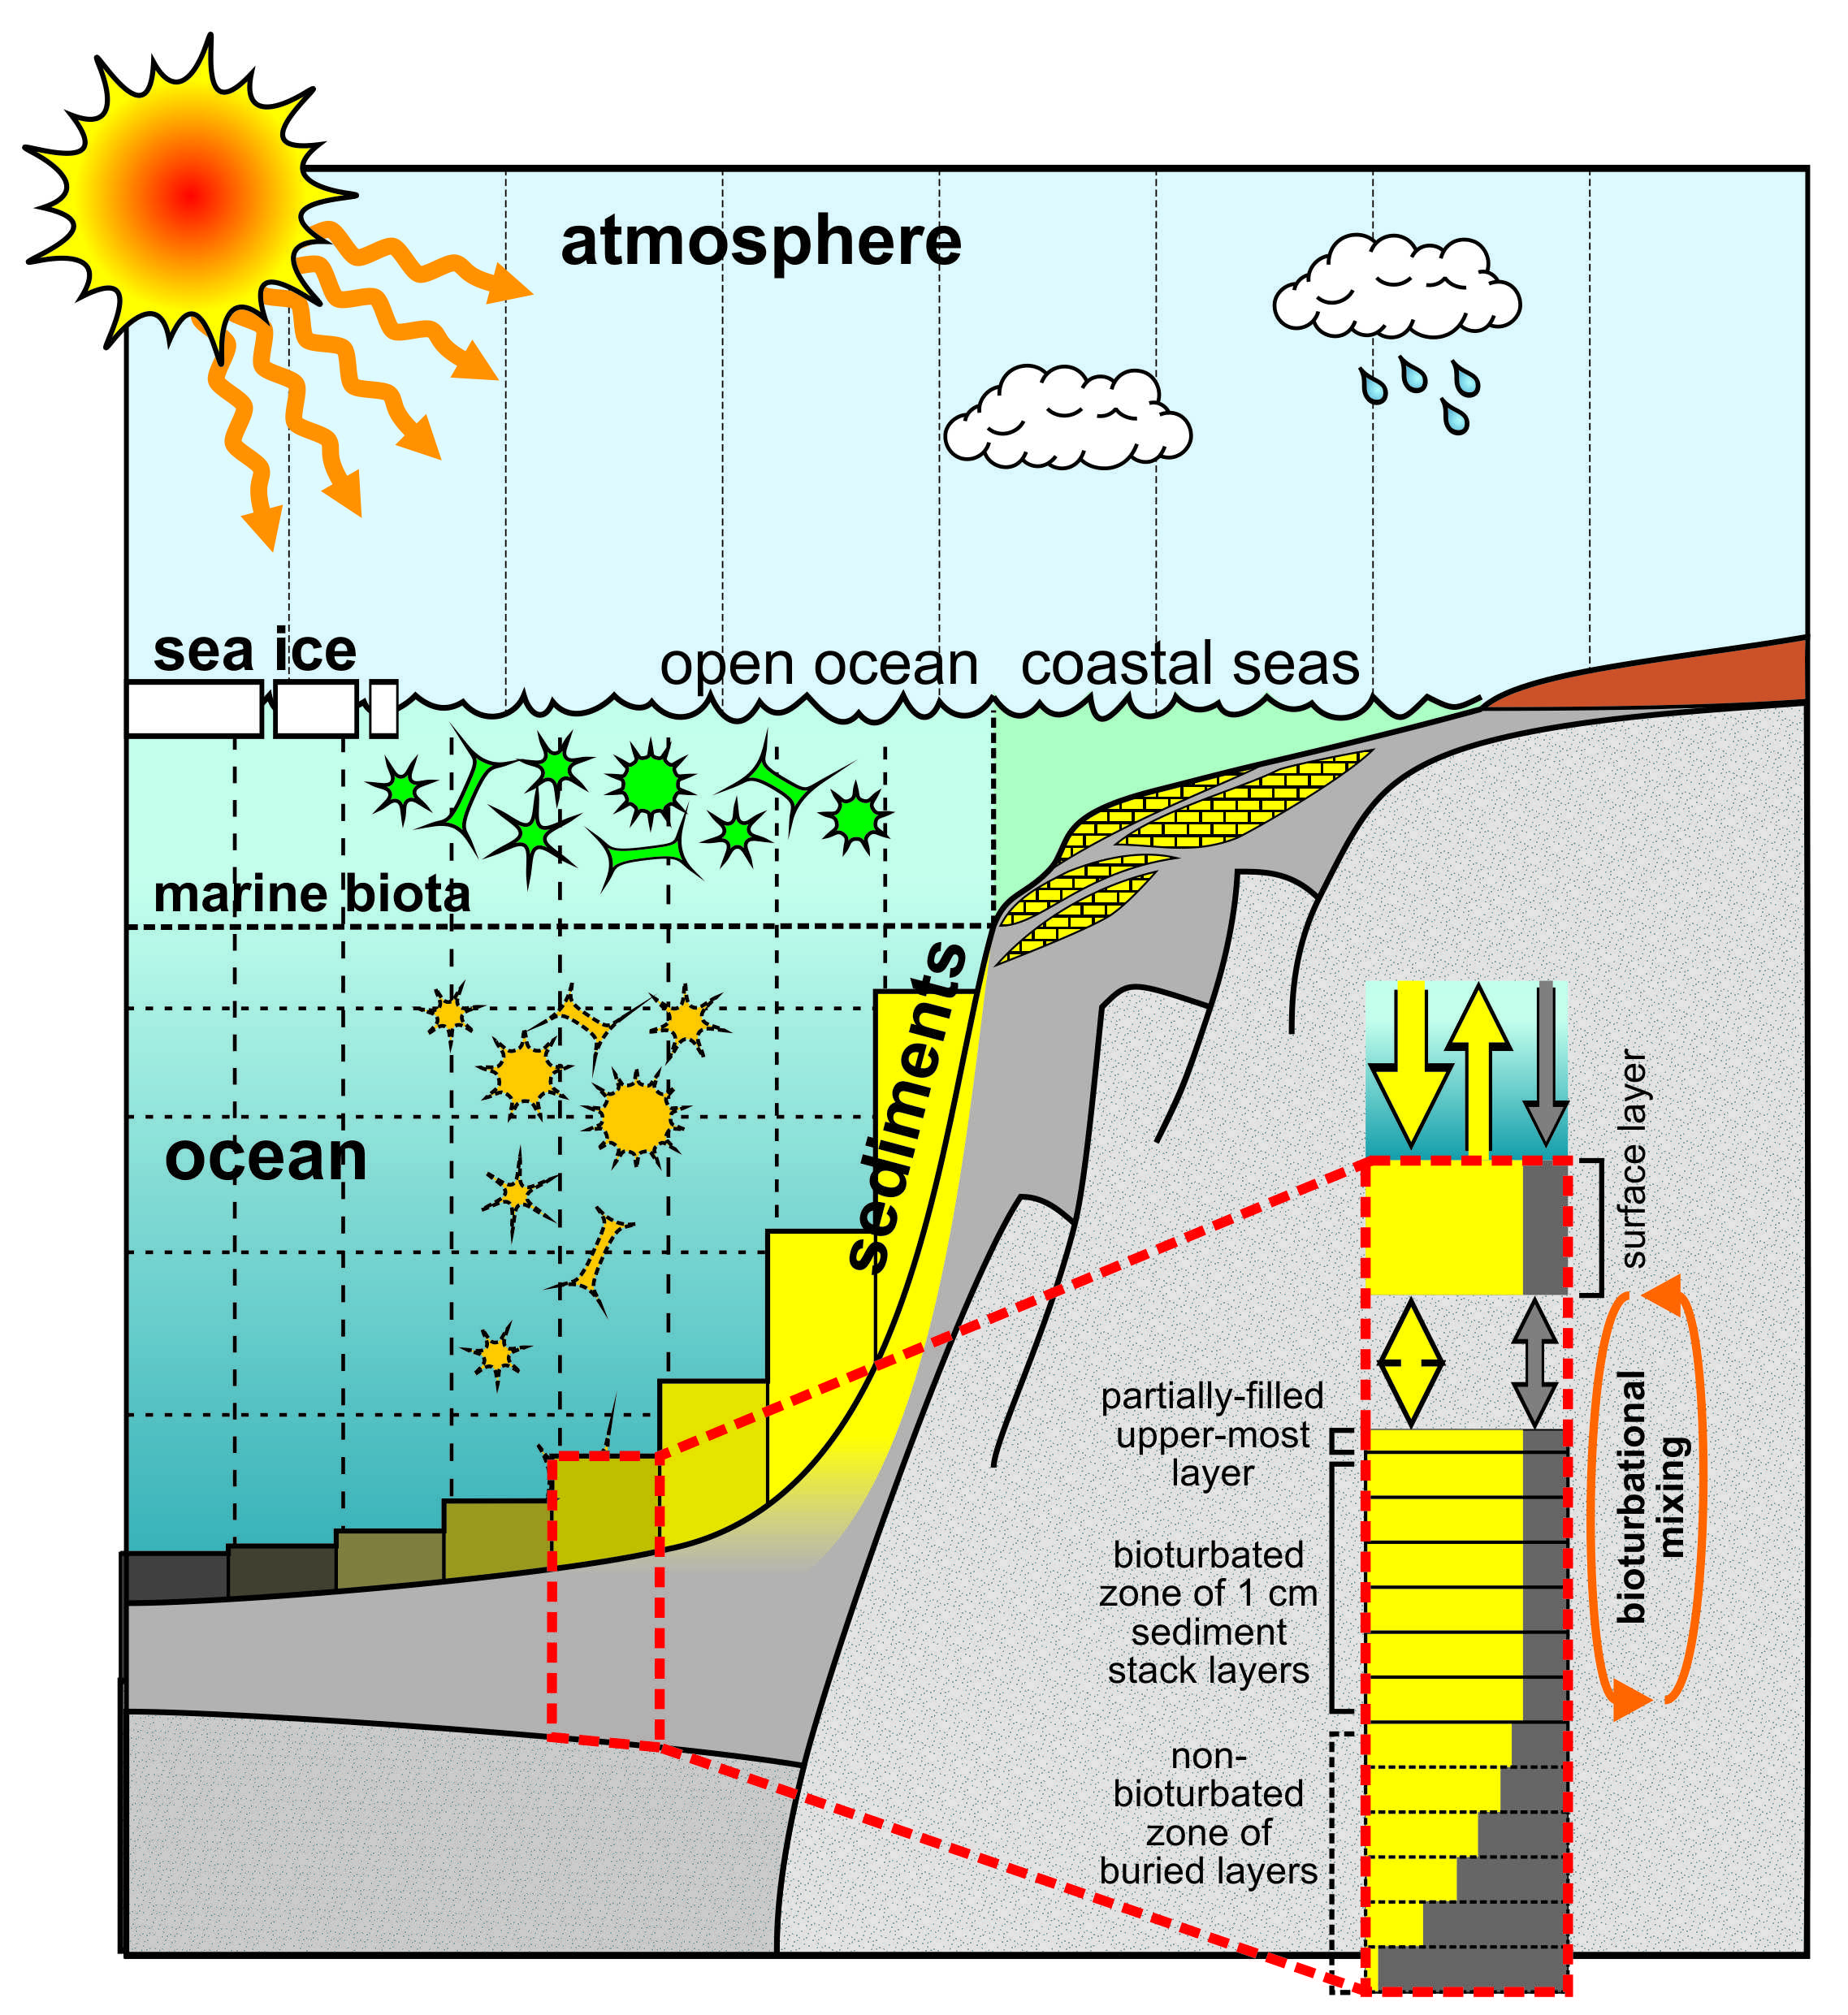
\includegraphics[width=0.5\textwidth]{sediments.jpg}
\caption{Schematic of \textbf{SEDGEM} sediment component.}
\label{fig:sediments}
\end{figure}

\vspace{1mm}
\noindent\rule{4cm}{0.1mm}
\vspace{2mm}

\noindent Take the new model configuration for a test drive by running on from the provided \textit{re-start} experiment: \textsf{\footnotesize EXAMPLE.\_rwlma.PO4\_S18x18.SPIN2.tar.gz}.

This is a steady-state climate+carbon cycle experiment that includes the deposition of \(CaCO_{3}\) in deep-sea sediments as well as the balance between weathering (solute input to the ocean) and burial (output), which in this case, are in fact in balance (because the model has been run for 50,000 years to ensure this ...). Try running ('briefly', but 100 years would not be too tedious for this faster configuration!):
\vspace{-2mm}\begin{verbatim}
$ ./runmuffin.sh cgenie.eb_go_gs_ac_bg_sg_rg_gl._rwlma.BASES
 LABS LAB_11.EXAMPLE 100 EXAMPLE._rwlma.PO4_S18x18.SPIN2
\end{verbatim}\vspace{-2mm}
Note that the \textit{base-config} file \textsf{\footnotesize cgenie.eb\_go\_gs\_ac\_bg\_sg\_rg\_gl.\_rwlma.BASE} specifies the use of a sediment model -- the ‘\textsf{\footnotesize sg}’ in the filename.
Also note that we are running at a degraded (lower) \(18\times18\) resolution, and requiring fewer (twice as few in fact!) time-steps per year, for an overall approximately order-of-magnitude decrease in run-time as compared to a standard  \(36\times36\) resolution configuration of \textbf{muffin}. This is extremely helpful in being able to run \textbf{muffin} on geological time-scales but within a reasonable about of real time. (The configuration also utilizes a conceptual/idealized continental configuration somewhat similar to as in the snowball Earth experiments.)

The \textit{user-config} \textsf{\footnotesize LAB\_11.EXAMPLE } is set up with the global carbon cycle configured as 'open' -- that is to say, that there is an input of carbon (and alkalinity) to the ocean from weathering, and a loss due to preservation and burial of \(CaCO_{3}\) in deep-sea sediments. Depending on the state of ocean chemistry (and biology) and weathering, these two fluxes (input vs. output) do not have to balance, and hence ocean carbonate chemistry (and in turn, atmospheric \(pCO_{2}\)) can evolve with time. The \textit{spin-up} may not necessarily have the two fluxes perfectly balanced and hence before you run any experiments you might want to confirm whether the spin-up provided really is adequately 'spun-up'\footnote{i.e. you might plot some of the variables from the results of the \textit{spin-up}  experiment as a function of time and judge whether they are sufficiently converged or not.}.

Note that a residual drift can be dealt with if it is relatively small and near linear via the use of a \uline{control experiment}, because any experiment you carry out will likely also incorporate (or be biased) by the same residual drift. Running a control gives you something to directly contrast  your experiment with and calculating the difference (e.g., a difference map or simple subtraction of global numbers) will give you the effect of whatever parameters you changed in the experiment but corrected for any drift. In previous exercises, we were a little lazy, and difference maps were often created with respect to year 1 of an experiment -- strictly, they should have been created relative to the same year of a parallel control experiment, i.e., results at year 100 should have been contrasted with the year 100 results of the control.

%------------------------------------------------

\newpage

%------------------------------------------------

\section{Sediment model output}

There is a whole new set of additional outputs from this configuration of \textbf{muffin}, particularly sediment-specific output from the \textbf{SEDGEM} module and which is saved in the \textsf{\footnotesize sedgem } sub-directory of the main experiments results directory. Data saving differs from  \textbf{BIOGEM} in that the composition of the sediments (and other diagnostics such as rain and dissolution fluxes) is saved only \uline{at the very end} of a model experiment (hence unlike \textbf{BIOGEM}, which by default saves a series of time-slices throughout the course of a model experiment). So if you kill a run before the very end (or the run crashes),  \uline{you will get no} (or little) \textbf{SEDGEM} output.

2D (e.g. surface sediment properties, fluxes, etc.) results can be found in  the \textsf{\footnotesize sedgem } sub-directory of your experiment directory  in a netCDF file called \textsf{\footnotesize fields\_sedgem\_2d.nc}. (Note that there is some duplication of results saving, because a series of \textit{time-slices} of sediment composition are also saved in the 2D \textbf{BIOGEM} netCDF file \textsf{\footnotesize fields\_biogem\_2d.nc}. \textbf{BIOGEM} also saves a selection of \textit{time-series }of sediment properties -- \textsf{\footnotesize .res } files starting \textsf{\footnotesize biogem\_series\_sed}. For example, the \textit{time-series} file: \textsf{\footnotesize biogem\_series\_sed\_CaCO3.res }  contains information about how the mean \(CaCO_{3}\) content of surface sediments (uppermost sediment layer) evolves with time.

The 2D distribution of \(wt\% CaCO_{3}\) – which is the weight fraction of calcium carbonate (\(CaCO_{3}\)) in the surface sediments of the deep ocean (i.e., how much plankton carbonate shell material is there compared to other stuff in the mud at the bottom of the ocean) is saved under a variable called: \textsf{\footnotesize sed\_CaCO3}.

\vspace{1mm}
\noindent\rule{4cm}{0.1mm}
\vspace{2mm}

\noindent The model also generates artificial sediment ‘cores’ (e.g. see: \textit{Ridgwell} [2007]) and hence what one might expect to see of your applied perturbations as recorded in a sediment core sand then recovered from the ocean floor(!) In the \textbf{SEDGEM} results sub-directory, there is a netCDF file which contains all the locations selected (if any) –- \textsf{\footnotesize sedcore.nc}. These are not really aligned with latitude as the \textbf{Panoply} display might suggest – the locations are in fact distributed from all over the ocean (\textbf{Panoply} is being fooled in order to display them together). In the \textbf{SEDGEM} 2D netCDF file, these locations are marked in the netCDF variable \textsf{\footnotesize grid\_mask\_sedcore}. The locations of these cores are stored in a a file containing a little ASCII ‘map’ of the ocean.
\vspace{1mm}

\begin{itemize}[noitemsep]
\vspace{1mm}
\item
If you are using a 'paleo' configuration of \textbf{muffin}, indicated by a parameter section in the \textit{base-config} file headed by something looking like:
\footnotesize\begin{verbatim}
# *******************************************************************
# GRID & BOUNDARY CONDITION CONFIGURATION
# *******************************************************************
# insert the automatically generated muffingen parameter list here
# *******************************************************************
###################################################################################
### cGENIE .config file parameter lines generated by muffingen v0.84 on: 191119 ###
\end{verbatim}\normalsize
then there will be a parameter line that direct muffin to look for \textbf{SEDGEM} configuration files in the respective \textsf{\footnotesize genie-paleo } directory, e.g.:
\vspace{-1mm}\small\begin{verbatim}
sg_par_pindir_name='../../cgenie.muffin/genie-paleo/fkh_pp03/'
\end{verbatim}\normalsize\vspace{-1mm}
\vspace{1mm}
\item Otherwise, the file lives in: \textsf{\footnotesize cgenie.muffin/genie-sedgem/data/input}
\end{itemize}
\vspace{1mm}
The filename is given by the parameter: \texttt{sg\_par\_sedcore\_save\_mask\_name}
\\Simply be editing (using the ASCII text editor) a ‘0.0’ to a ‘1.0’, you can get the model to generate and save a sediment ‘core’ at that particular (\textit{i,j}) location.

\pagebreak

\noindent netCDF file \textsf{\footnotesize sedcore.nc } variables include:

\vspace{1mm}
\begin{itemize}[noitemsep]
\item \textsf{\footnotesize phys\_layer } –- sediment layer number (counting down).
\item \textsf{\footnotesize phys\_depth } -– (cumulative) depth below surface, measured from the sediment surface to the mid-point of each sediment layer (cm).
\item \textsf{\footnotesize th (cm) } -- thickness of each sediment layer (cm).
\item \textsf{\footnotesize age\_CaCO3 } -- the mean age of \(CaCO_{3}\) particles in a sediment layer.
\\Note that this will not be defined if there is no \(CaCO_{3}\) preserved.
\item \textsf{\footnotesize ... } then some alternative ways of assigning a chronology to a sediment core … (ignore) ...
\item \textsf{\footnotesize phys\_porosity  } -- sediment layer density (as if you cared!).
\item \textsf{\footnotesize sed\_POC } and \textsf{\footnotesize sed\_POC\_13C } -- mean organic matter content of each sediment layer and its \(\delta^{13} C\). But note: in this configuration no organic matter is preserved (hence all zeros for POC).
\item \textsf{\footnotesize sed\_CaCO3} and \textsf{\footnotesize sed\_CaCO3\_13C } -- mean \(CaCO_{3}\) content (wt\%) of each sediment layer and its \(\delta^{13} C\).
\item \textsf{\footnotesize sed\_det } and \textsf{\footnotesize sed\_ash } -- the wt\% detrital and ‘ash’ contents of a layer (ash is used as a conservative numerical sediment tracer in order to mark the depth of the start of the experiment).
\end{itemize}
\vspace{1mm}

\noindent Obviously – you could plot e.g. \(CaCO_{3}\) (or its \(\delta^{13}C\)) as a function of depth and/or age across and see how your carbon release experiment might be recorded in the marine geological record (e.g. how does this compare with observations across the PETM?).

Note that the sediment cores reflect not only the material which has accumulated (or not, if it has dissolved …) during the course of your experiment, but also the material that accumulated during the 50,000 year spin-up. PLUS, whatever material the sediment core was initialized with to start with. For example, the large interval of initially 100\% detrital material at the base of the sediment core  simply reflects the initialization of the sediment array in the model. 

Also note the ash ‘peak’ near the bottom of the stack (filled) sediment layers – this is a tracer to ‘tag’ the start of the model spin-up. If you look at the spin-up results (not your recent perturbation experiment) – the ash peak lies in a sediment layer with age 50,000 years. But why is there any ash deeper than the age corresponding to the start of the spin-up? How can it get there (i.e. what processes could move solid material deeper within the sediment column)?

%------------------------------------------------

\newpage

%------------------------------------------------

\section{Quantifying how long is the long tail of CO$_{2}$}

You are now considering a rather more complex carbon cycle than before (e.g. now including a number of additional, mostly sediments/weathering processes). It is hence worth conducting some idealized perturbations of the global carbon cycle to get a feel for the sensitivity and time-scale of the (now 'geological') system response.

For instance – one illustrative experiment, and which has a parallel to experiments you have conducted previously, is to add a pulse \(CO_{2}\) release to the atmosphere and track the consequences for atmospheric p\(CO_{2}\) and ocean chemistry (particularly ‘alkalinity’), and now also e.g. deep sea sediments. To the \textsf{\footnotesize LAB\_11.EXAMPLE} \textit{user-config}, add the lines:
\vspace{-1mm}\small\begin{verbatim}
bg_par_forcing_name='pyyyyz.FpCO2_Fp13CO2'
bg_par_atm_force_scale_val_3=8.3333e+016
bg_par_atm_force_scale_val_4=-27.0
\end{verbatim}\normalsize\vspace{-1mm}
in order to achieve a 1000 PgC total release in a single year (or multiply by 5 to be comparable-ish to the 5000 PgC release in \textit{Ridgwell and Hargreaves} [2007]) with an isotopic composition of \(-27\)\permille -- appropriate for a fossil fuel carbon source. For reference -- methane derived carbon (e.g. as from hydrates) would be more like  \(-60\)\permille.

BE CAREFUL -- if you have previously edited files of the \textit{forcing} \textsf{\footnotesize  pyyyyz.FpCO2\_Fp13CO2 }, you are going to need to return whatever you have edited back to its original state. Or, carry out the following procedure:
\begin{enumerate}[noitemsep]
\vspace{1mm}
\item From \textsf{\footnotesize genie-main}, \texttt{\$ make cleanall}
\vspace{1mm}
\item Then head up a directory level (\texttt{cd ..}) to \textsf{\footnotesize cgenie.muffin}
\vspace{1mm}
\item Type: \texttt{\$ git status -uno}
\\You should see a list of all files that you originally installed (cloned from GitHub) that you have changed. e.g. you might see:
\vspace{-1mm}\small\begin{verbatim}
modified:   genie-forcings/pyyyyz.FpCO2_Fp13CO2/biogem_force_flux_atm_pCO2_sig.dat
\end{verbatim}\normalsize\vspace{-1mm}
(Note that file you create are not listed. TO see those, type: \texttt{\$ git status})
\vspace{1mm}
\item To restore the state of any file that you might have edited, \texttt{git checkout} that file out, e.g.:
\vspace{-1mm}\small\begin{verbatim}
$ git checkout genie-forcings/pyyyyz.FpCO2_Fp13CO2/biogem_force_flux_atm_pCO2_sig.dat
\end{verbatim}\normalsize\vspace{-1mm}
\end{enumerate}
\vspace{1mm}
Or ... simply keep the units scale parameter set in the \textit{user-config}:
\vspace{-1mm}\small\begin{verbatim}
bg_par_atm_force_scale_val_3=8.3333e+013
\end{verbatim}\normalsize\vspace{-1mm}
as you have done earlier, and edit the number of \(PgC\:yr^{-1}\) in the \textit{forcing} time-series (\textsf{\footnotesize .sig}) file. (You still might want to restore the forcing file to its original state if you have previously edited it.)

\vspace{1mm}
\noindent Run the model for as long as you dare (or can be bothered) – 1,000 or 2,000 years might be just enough  to start to see impacts on deep-sea sediments, but 5,000 or 10,000 years would be much better. (You can always submit this to the cluster queue and get on with something else.) FYI: 10,000 years is going to take something like an hour ... if you are lucky ...

Plot the time-series of e.g. atmospheric \(pCO_{2}\) and compare to the (much shorter experiments) you have carried out before with a simple ocean+atmosphere only system. Compare how quickly atmospheric \(pCO_{2}\) decays compared to previously \textbf{muffin} publications\footnote{see: http://www.seao2.info/pubs.html} (e.g. \textit{Ridgwell and Hargreaves} [2007]) or other models (e.g. \textit{Archer et al.} [2009]) and  how the sediments respond (e.g. the time-series of sediment \(CaCO_{3}\) content).

\vspace{1mm}
\noindent\rule{4cm}{0.1mm}
\vspace{2mm}

\vspace{4mm}
\pagebreak

\noindent To properly (quantitatively) appreciate the role of ocean-sediment interaction (and weathering) and controlling atmospheric \(pCO_{2}\), you need to contrast these experiments with as similar a model configuration as possible -- for instance, one that is identical excepting having no sediments (or weathering). You can achieve this quite simply: create (/copy-rename) a new \textit{user-config} based on \textsf{\footnotesize LAB\_x.sediments }and edit the lines\footnote{You do not have to edit the comment line (\#) but it will help you remember what you have done.}:
\vspace{-1mm}\small\begin{verbatim}
# set an 'OPEN' system
bg_ctrl_force_sed_closedsystem=.false.
\end{verbatim}\normalsize\vspace{-1mm}
changing it to:
\vspace{-1mm}\small\begin{verbatim}
# set a 'CLOSED' system
bg_ctrl_force_sed_closedsystem=.true.
\end{verbatim}\normalsize\vspace{-1mm}

\noindent What this  does is to force the model to always maintain an exact balance between the preservation and burial in marine sediments of \(CaCO_{3}\), with the supply of solutes derived from the weathering of \(CaCO_{3}\) on land. Because no excess or deficit of  weathering vs. sedimentation is  allowed to occur, no changes in ocean chemistry (other than by air-sea gas exchange) occur. This configuration hence acts (geochemically and dynamically) exactly the same way as a configuration without any sediments or weathering being present (and as used previously). By comparing the two experiments: can you deduce the effect of the sediments in modulating (accelerating or decelerating) atmospheric \(pCO_{2}\) decline?\footnote{e.g. you could compare the \(pCO_{2}\) time-series of the 2 different experiments.}

Also view the sediment distribution (of \(CaCO_{3}\)): what are the impacts on sediment composition in the case of an experiment configured with an ‘open’ system (vs. a 'closed' system)? Here, the time-series file of mean global sediment composition \textsf{\footnotesize biogem\_series\_sed\_CaCO3.res} (in units of: \(wt\%\:CaCO_{3}\)) may help illustrate what is going on here.
Note that the way the ‘closed’ system is constructed; a response of the sediments is predicted and saved in the output, even though it is not allowed to affect chemistry or atmospheric p\(CO_{2}\).

To recap -- you are aiming to run a \(CO_{2}\) emissions experiment using a \textbf{muffin} configuration including variable weathering and sedimentation (\textsf{\footnotesize LAB\_11.EXAMPLE }) with a version/copy that you have edited to create a 'closed' ocean-atmosphere system, with no ocean-sediment or weather feedbacks on atmospheric \(CO_{2}\). Ideally, you would also run a pair of control experiments -- both 'open' and 'closed' configurations but with no \(CO_{2}\) emissions specified. (A total of 4 experiments.)

%------------------------------------------------

\newpage

%------------------------------------------------

\section{Sediments of the modern Earth}

Important is to critically and quantitatively assess to what degree \textbf{muffin}  provides an adequate representation of the interaction between ocean chemistry and sediment composition (e.g., in CaCO3 buffering of \(CO_{2}\) release and 'carbonate compensation'). Key to this, is contrasting  model output against observational-based data. Such an approach is presented in \textit{Ridgwell and Hargreaves} [2007].

The required \textit{base-} and \textit{user-config} files are provided as part of the \textbf{muffin} code release:

\begin{itemize}[noitemsep]
\vspace{1mm}
\item \textsf{\footnotesize cgenie.eb\_go\_gs\_ac\_bg\_sg\_rg.worbe2.BASE } -- the \textit{base-config} file, including \textbf{SEDGEM} and \textbf{ROKGEM} modules.
\vspace{1mm}
\item \textsf{\footnotesize EXAMPLE.worbe2.RidgwellHargreaves1997\_S36x36.SPIN1 } -- the \textit{user-config} for the 1st stage (20 kyr long) \textit{spin-up} described in  \textit{Ridgwell and Hargreaves} [2007]. This file lives in the \textsf{\footnotesize genie-userconfigs } sub-directory.
\\\textsf{\footnotesize EXAMPLE.worbe2.RidgwellHargreaves1997\_S36x36.SPIN2 } is the 2nd-stage, 50 kyr \textit{spin-up} that uses \textsf{\footnotesize EXAMPLE.worbe2.RidgwellHargreaves1997\_S36x36.SPIN1 } as a \textit{re-start}.
\end{itemize}
\vspace{1mm}
e.g. you would run the 2 experiments, one after the other:
\vspace{-1mm}\small\begin{verbatim}
./runmuffin.sh cgenie.eb_go_gs_ac_bg_sg_rg.worbe2.BASE /
   EXAMPLE.worbe2.RidgwellHargreaves1997_S36x36.SPIN1 20000
\end{verbatim}\normalsize\vspace{-2mm}
\vspace{-2mm}\small\begin{verbatim}
./runmuffin.sh cgenie.eb_go_gs_ac_bg_sg_rg.worbe2.BASE /
   EXAMPLE.worbe2.RidgwellHargreaves1997_S36x36.SPIN2 50000
   EXAMPLE.worbe2.RidgwellHargreaves1997_S36x36.SPIN1
\end{verbatim}\normalsize\vspace{-1mm}

Does the model get the broad patterns right (is it more right than wrong, or more wrong than right)? Do you think the model-data misfits might be important?

\vspace{1mm}
(Pre-run experiments of the same name are also provided from: \textsf{\footnotesize  http://www.seao2.info/cgenie\_output/})

%------------------------------------------------

\newpage

%------------------------------------------------

\section{The marine geology of fake worlds}

You can configure any of your previous fake worlds, or generate new ones, to have a full geologic carbon cycle including deposition of \(CaCO_{3}\) in marine sediments and weathering on land.

In order to generate the requisite \textbf{SEDGEM} configuration files, you need the following settings in your \textbf{muffingen} configuration file:

\begin{itemize}[noitemsep]
\vspace{1mm}
\item \texttt{opt\_makeseds=true;} --  requests that \textbf{SEDGEM} files are generated.
\vspace{1mm}
\item \texttt{par\_sedsopt=2;} -- requests that a randomized bathymetry is generated. This is needed because fake worlds have by default, a flat bathymetry.
\\Instead, if you 'draw' a non-uniform bathymetry, you would set:
\\ \texttt{par\_sedsopt=0;} -- requests that the ocean depth levels ('k1' file') are used to inform the ocean floor depth assumed by \textbf{SEDGEM}.
\\(Option \texttt{1} is most commonly used in conjunction with a GCM-derived continental configuration.)
\end{itemize}

\vspace{1mm}
So, if you define continents in your fake world, but do not change the bathymetry in \textbf{muffingen}, \texttt{par\_sedsopt} option \texttt{2} will give you a randomized distribution of sediment depths (used in the \(CaCO_{3}\) solubility pressure calculation only). Selecting option \texttt{0} will simply translate your chosen \textbf{muffingen} ocean depths into \textbf{SEDGEM} depths. Note that you can still have a flat bottom to the ocean (no variation in ocean floor depth) and choose option \texttt{0}.

If you define a specific bathymetry by hand (e.g. draw in ocean ridges), you probably do not want it over-written (by a random \textbf{SEDGEM} depth pattern) and hence you should chose option \texttt{0}.

For speed of running model experiments, it is recommended that you generate your \textbf{muffingen} \textbf{muffin} configurations at the lowest reasonable resolution -- \(18\times18\times8\) would be suitable -- \(18\times18\) resolution in lon vs. lat, and \(8\) levels in the ocean. (You could try pushing this a little further and more extreme, e.g. \(12\times12\times8\).) Note that when you create your \textit{base-config}, you should use the template:
\vspace{1mm}
\\\textsf{\footnotesize CONFIG\_template\_08lvl\_R07.config}
\vspace{1mm}
\\(for the 8-level ocean, rather than \textsf{\footnotesize CONFIG\_template\_16lvl\_R07.config } which is designed for 16-ocean level configurations).

Once you have copy-pasted the configuration output of \textbf{muffingen} into the template \textit{base-config} file (and suitably renamed it), you need to enable the geologic carbon cycle modules (\textbf{SEDGEM} and \textbf{ROCKGEM}). At the top of the \textit{base-config} file, ensure that the following are set:
\vspace{-1mm}\small\begin{verbatim}
ma_flag_sedgem=.TRUE.
ma_flag_rokgem=.TRUE.
\end{verbatim}\normalsize\vspace{-1mm}
And then, further down and under the heading:
\vspace{-1mm}\small\begin{verbatim}
# TRACER CONFIGURATION
\end{verbatim}\normalsize\vspace{-1mm}
you need to define how many 'tracers' in the ocean, what they are, and any initial values that differ from modern defaults. Plus, whatever atmospheric and sediment tracers you want (plus default values in the atmosphere). Simplest at this point is to copy-paste from an existing \textit{base-config}, such as:
\vspace{1mm}
\\\textsf{\footnotesize cgenie.eb\_go\_gs\_ac\_bg\_sg\_rg.worbe2.BASE}
\vspace{1mm}
\\(which is the \textit{base-config} used in \textit{Ridgwell and Hargreaves} [2007]).

\vspace{1mm}
As for a suitable \textit{user-config} ...

... you could take the \textit{user-config} from \textit{Colbourn et al.} [2013] (itself a modification of Ridgwell and Hargreaves [2007]) -- available as part of the \textbf{muffin} code release, as file:
\vspace{1mm}
\\\textsf{\footnotesize EXAMPLE.worbe2.Colbournetal2013.CTRL } (\textsf{\footnotesize genie-userconfigs } sub-directory)
\vspace{1mm}
\\Then generalize this according to the paleo sediment configuration used in \textit{Ridgwell and Schmidt} [2010] (file: \textsf{\footnotesize EXAMPLE.p0055c.RidgwellSchmidt2010.SPIN1 } in the \textsf{\footnotesize genie-userconfigs } sub-directory) (i.e. making \(CaCO_{3}/POC\) export invariant, adding a fixed detrital flux to the sediments).

Cutting the lines down to the bare minimum (excepting comments pertaining to new/altered lines), a suitable \textit{user-config} then looks like:

\scriptsize\begin{verbatim}
# --- CLIMATE --------------------------------------------------
# enable CO2 climate feedback
ea_36=y
# --- BIOLOGICAL NEW PRODUCTION --------------------------------
bg_par_bio_k0_PO4=1.9582242E-06
bg_par_bio_c0_PO4=2.1989611E-07
# --- ORGANIC MATTER EXPORT RATIOS -----------------------------
bg_par_bio_red_DOMfrac=0.66
# --- INORGANIC MATTER EXPORT RATIOS ---------------------------
# set fixed export CaCO3 as a proportion of particulate organic matter
bg_par_bio_red_POC_CaCO3=0.200
bg_par_bio_red_POC_CaCO3_pP=0.0
# --- REMINERALIZATION -----------------------------------------
bg_par_bio_remin_DOMlifetime=0.5
bg_par_bio_remin_POC_frac2=6.4591110E-02
bg_par_bio_remin_POC_eL1=550.5195
bg_par_bio_remin_POC_eL2=1000000.0
bg_par_bio_remin_CaCO3_frac2=0.468
bg_par_bio_remin_CaCO3_eL1=1083.486
bg_par_bio_remin_CaCO3_eL2=1000000.0
# --- SEDIMENTS ------------------------------------------------
# sediment diagenesis options
sg_par_sed_diagen_CaCO3opt="ridgwell2001lookup"
sg_ctrl_sed_bioturb=.true.
sg_ctrl_sed_bioturb_Archer=.false.
sg_par_n_sed_mix=20
sg_par_sed_mix_k_sur_max=0.15
sg_par_sed_mix_k_sur_min=0.15
# additional detrital flux (g cm-2 kyr-1)
sg_par_sed_fdet=0.180
# --- WEATHERING -----------------------------------------------
# set a 'OPEN' system
bg_ctrl_force_sed_closedsystem=.false.
# set CaCO3_weathering-temperature feedback
rg_opt_weather_T_Ca=.TRUE.
# set CaSiO3_weathering-temperature feedback
rg_opt_weather_T_Si=.TRUE.
# weathering reference mean global land surface temperature (C)
rg_par_ref_T0=8.48
#CO2 outgassing rate (mol C yr-1)
rg_par_outgas_CO2=5.59E+12
# global silicate weathering rate (mol Ca2+ yr-1)
rg_par_weather_CaSiO3=5.59E+12
# global carbonate weathering rate (mol Ca2+ yr-1)
rg_par_weather_CaCO3=5.59E+12
# d13C
rg_par_outgas_CO2_d13C=-6.0
rg_par_weather_CaCO3_d13C=12.8
# --- DATA SAVING ----------------------------------------------
bg_par_data_save_level=4
bg_ctrl_debug_lvl0=.true.
ma_debug_loop=1
# --- END ------------------------------------------------------
\end{verbatim}\normalsize

Here, the reference temperature against which  the rate of weathering is modified for higher/lower temperatures, is set for a modern-like continental configuration:
\vspace{-1mm}\small\begin{verbatim}
# weathering reference mean global land surface temperature (C)
rg_par_ref_T0=8.48
\end{verbatim}\normalsize\vspace{-1mm}
If left un-changed, then the negative silicate weathering feedback will operate on atmospheric \(CO_{2}\) -- letting it accumulate, or removing it, until the reference temperature is achieved. If instead, you want to achieve a specific atmospheric \(CO_{2}\) at steady state, you need to know the relevant mean global land surface temperature. To determine this -- first run \textbf{muffin} with a prescribed atmospheric \(CO_{2}\) value, e.g. by adding:
\vspace{-1mm}\small\begin{verbatim}
# --- FORCINGS -------------------------------------------------
# specify forcings
bg_par_forcing_name="pyyyyz.RpCO2_Rp13CO2"
bg_par_atm_force_scale_val_3=278.0E-06
bg_par_atm_force_scale_val_4=-6.5
\end{verbatim}\normalsize\vspace{-1mm}
(or some other value of \(CO_{2}\)) to your \textit{user-config}. Running the model for about 1000 years should be more than enough to achieve a near steady-state of surface climate, allowing to read off the mean global surface air temperature over land (BIOGEM file \textsf{\footnotesize biogem\_series\_misc\_SLT.res}), and set the reference temperature to this value. You can then run an experiment without a prescribed atmospheric \(CO_{2}\) forcing, now knowing that the silicate weathering feedback will always act to restore atmospheric \(CO_{2}\) back to that value.

\vspace{1mm}
\noindent\rule{4cm}{0.5pt}
\vspace{2mm}

\noindent Despite the low grid resolution, this is still  going to take a l o n g time for particularly much to happen and you could probably do with some (numerical) 'help'. You can accelerate the run-time of \textbf{muffin} in calculating the balance between weathering and sedimentation, a-la \textit{Lord et al.} [2015]. To do this, you need to add a new section of parameter choices to the \textit{user-config} file:
\vspace{-1mm}\small\begin{verbatim}
# --- GEOCHEM ACCELERATION -------------------------------------
gl_ctrl_update_pCO2=.true.
ma_gem_notyr_min=10
ma_gem_notyr_max=10
ma_gem_yr_min=90
ma_gem_yr_max=90
ma_gem_dyr=0
ma_gem_adapt_auto=.false.
\end{verbatim}\normalsize\vspace{-1mm}
Here, this specifies that you would like to spend only \(10\) years of full updating of the model for each \(90\) years spent in an accelerated calculation which treats the entire ocean as if it were a single geochemical reservoir (see: \textit{Lord et al.} [2015]) -- an almost \(10:1\) acceleration and reduction in experiment run-time. (But note that the ocean circulation and ocean carbon and nutrient cycles will appear to be taking longer to come to equilibrium because they are only being fully updated \(10\) years in every \(100\).

Note that this acceleration is good for spin-ups and determining equilibrium weathering-sedimentation states, but not so useful for transient \(CO_{2}\) changes (see in \textit{Lord et al.} [2015] for how a less acceleration and adaptive setup had to be used). Similarly, acceleration is not so useful for varying orbits experiments.

\vspace{1mm}
\noindent\rule{4cm}{0.5pt}
\vspace{2mm}

\noindent A couple of different possible experimental investigations follow.\footnote{Note that in using the given \textit{user-config} settings, steady state is only reach after several 100 kyr (which is going to take a while, even at low resolution and with acceleration). Regardless of your assumptions regarding sea-floor bathymetry, you should find that atmospheric \(CO_{2}\) always reaches the same value.
}
\begin{enumerate}[noitemsep]

\vspace{1mm}
\item Firstly, you could simply test what happens if there is no sediment surface depth variability as compared to a configuration with depth (pressure) variability in sediment surface depth (and one that follows a modern-like distribution of depth vs. area). The science question would be something like -- how important is a distribution of ocean depths to setting the steady state alkalinity (or saturation) of the ocean? Or: in having an appreciable amount of shallower sea-floor where \(CaCO_{3}\) will be preserved and buried much more readily -- how much less saturated must the ocean as a whole become in order to balance weathering and sedimentation?
\\F or this, you'll need 2 \textbf{muffingen} configurations, each with the same continental configuration, but one generated with random sediment depths, and one with a uniform depth.
\\Simplest, but more tedious, is to run \textbf{muffingen} twice, with your  configuration settings files differing only in the value of \texttt{par\_sedsopt}. However, faster is to generate one configuration using the configuration template \textsf{\footnotesize EXAMPLE\_BLANK.m}, and then generate a 2nd one, using the 'k1' file generated by the first \textbf{muffingen} \textbf{muffin} generation. An example of creating a \textbf{muffin} configuration from a 'k1' file is: \textsf{\footnotesize EXAMPLE\_K1\_permian.m}. Basically, the only thing that changes between the first and second \textbf{muffingen} \textbf{muffin} generation, in addition to \texttt{par\_sedsopt}, is the value of \texttt{par\_gcm}, which changes from \texttt{''} (empty) in \textsf{\footnotesize EXAMPLE\_BLANK.m}, to \texttt{'k1'} in \textsf{\footnotesize EXAMPLE\_K1\_permian.m}.

\vspace{1mm}
\item As a variant on the above -- you might 'draw' a large and relatively shallow (e.g. 1 or 2 km depth)\ sea-floor plateau, run the model, and determine how much this has influenced ocean chemistry, at steady state (remembering to fun an experiment with no sea-floor plateau in a second experiment as a control).

\vspace{1mm}
\item How important is continental configuration and the position of the continents in controlling atmospheric \(CO_{2}\) via weathering?
\\You might, for instance, create 2 different continental configurations in \textbf{muffingen}, both with the same cratonic (land surface) area, and explore whether you achieve a different steady state atmospheric \(CO_{2}\) depending on whether the continent is at the pole, or centered on the equator. Remember that the parameterized silicate weathering feedback acts to restore global mean surface air temperature over land, to the reference value.\footnote{Note that the simple weathering parameterization in \textbf{muffin} does not care how much land there is, only what the mean surface air temperature over that land is.} You might then guess the sign of the change in atmospheric \(CO_{2}\) given that the weathering will act to restore the polar and equatorial continental temperatures to the same value and it does that by causing atmospheric \(CO_{2}\) to change. (But perhaps the magnitude of the effect will be unexpected, which is why you need a model.)

\end{enumerate}


%------------------------------------------------

\newpage

%------------------------------------------------

\section{Further ideas}

You might further explore the role of weathering and sensitivity the sensitivity of atmospheric \(pCO_{2}\) and climate to the strength  of the weathering feedback as well as to the assumed rate of volcanic \(CO_{2}\) outgassing, as well as how the products of weathering on land are accommodated through the burial (and pattern of burial) of \(CaCO_{3}\) in deep-sea sediments.
Parameters of ‘interest’ here, i.e. ones that you might adjust to explore the silicate weathering feedback and long-term controls on atmospheric \(pCO_{2}\), are listed under \texttt{\# --- WEATHERING ---}) in the \textit{user-config}, and include:
\vspace{1mm}
\begin{itemize}[noitemsep]
\item \texttt{rg\_par\_outgas\_CO2} -– the global \(CO_{2}\) outgassing rate in units of \(mol yr^{-1}\).
\item \texttt{rg\_par\_ref\_T0} -– the reference land surface temperature for weathering (units of \(^{\circ} C\)).
\end{itemize}
\vspace{1mm}

In \textbf{muffin}, global weathering rates will increase or decrease depending on whether the mean global surface temperature (which is reported and saved in \textbf{BIOGEM} \textit{time-series} output file: \textsf{\footnotesize biogem\_series\_misc\_SLT.res}). So, if you increase the reference temperature, weathering rates will drop and \(CO_{2}\) will accumulate in the atmosphere until the Earth was warmed sufficient that the mean global land surface temperature again matches the reference temperature. And \textit{vice versa} for the case of reducing the reference temperature. Maybe try a pair of experiments (plus a control in which you do not adjust the reference temperature) in which you adjust the value of \texttt{rg\_par\_ref\_T0} both up and down, to confirm this.

Conversely, increasing or decreasing the rate of \(CO_{2}\) outgassing should also act to increase or decrease, respectively, global temperatures (at steady state). Another pair of experiments (plus a 3rd, control) would be to try increasing and decreasing the value of \texttt{rg\_par\_outgas\_CO2}.

Now ... one problem concerns the time it is going to take the system to re-equilibrate to e.g. a different value of \(CO_{2}\) outgassing. For example, in \textit{Greene et al.} [2019]\footnote{ Greene, S.E., A. Ridgwell, S. Kirtland Turner, D.N. Schmidt, H. Pälike, E. Thomas, L.K. Greene, and B.A.A. Hoogakker, Early Cenozoic Decoupling of Climate and Carbonate Compensation Depth Trends, Paleoceanography and Paleoclimatology, 10.1029/2019PA003601 (2019).} (and in the Supporting Information data table S1 for the paper), you'll see time-series of the adjustment of atmospheric \(pCO_{2}\) in response to a change in outgassing rate. And then see it is a ca. 2 Myr time-scale to equilibrium ...

Help is at hand! And if you read the earlier fake world section, you can accelerate the time-to-equilibrium for systems such as these. Simply add, to your \textit{user-config}:

\vspace{-1mm}\small\begin{verbatim}
# --- GEOCHEM ACCELERATION -------------------------------------
gl_ctrl_update_pCO2=.true.
ma_gem_notyr_min=10
ma_gem_notyr_max=10
ma_gem_yr_min=990
ma_gem_yr_max=990
ma_gem_dyr=0
ma_gem_adapt_auto=.false.
\end{verbatim}\normalsize\vspace{-1mm}
Following \textit{Greene et al.} [2019] and as per the example \textit{user-config} files associated with this which can be found in: \textsf{\footnotesize genie-userconfigs/MS/greeneetal.2019} -- this specifies that you would like to spend only \(10\) years of full updating of the model for each \(990\) years spent in an accelerated calculation which treats the entire ocean as if it were a single geochemical reservoir (see: \textit{Lord et al.} [2015]) -- an almost \(100:1\) acceleration and reduction in experiment run-time. (But note that the ocean circulation and ocean carbon and nutrient cycles will appear to be taking longer to come to equilibrium because they are only being fully updated \(10\) years in every \(1000\).

\vspace{1mm}
\noindent\rule{4cm}{0.1mm}
\vspace{2mm}

\noindent Another pair of important controls on the preservation and burial of \(CaCO_{3}\) in marine sediments (but not one that ultimately at steady state, affects \(CO_{2}\) and climate), are the fluxes of \(CaCO_{3}\) and  organic carbon (POC) to the sediment surface.

All other things being equal -- increasing the export of \(CaCO_{3}\) and hence flux to the sediment surface requires that fraction of \(CaCO_{3}\) that dissolves increases at steady state. In other words -- instantaneously increasing the flux to the sediments of \(CaCO_{3}\) will increase burial relative to the weathering flux. The excess sink of \(CaCO_{3}\) will act to lower DIC and ALK (and \(Ca^{2+}\)), lowering the carbonate saturation state of the ocean, and reducing the preservation of \(CaCO_{3}\). This will continue up to the point where the preservation and burial of \(CaCO_{3}\) once again balances weathering.

An interesting question is what happens to atmospheric \(CO_{2}\). Ultimately it must return to its initial value due to the silicate weathering feedback. However, this occurs on a long (ca. 200 kyr) time-scale, whereas an imbalance between \(CaCO_{3}\) weathering and burial can act to change ocean chemistry on much shorter (1-10 kyr) time-scales. To explore this, you can adjust the parameter that sets the ratio of \(CaCO_{3}\) to POC export -- having the effect of changing the \(CaCO_{3}\) flux to the sediments whilst keeping everything else (almost) in the ocean carbon cycle invariant. The parameter is:
\vspace{-1mm}\small\begin{verbatim}
bg_par_bio_red_POC_CaCO3=0.200
\end{verbatim}\normalsize\vspace{-1mm}
Adjusting this value higher will increase the global export of \(CaCO_{3}\) from the surface ocean.

It is much more difficult to adjust the POC flux independent of \(CaCO_{3}\) (i.e. keeping the global \(CaCO_{3}\) flux invariant) because of the way muffin parameterizes biological \(CaCO_{3}\) export as a function of POC export. Without perturbing the ocean \(PO_{4}\) and hence productivity and carbon cycling too much, you can shift slightly more or less POC to a form that is assumed to reach the sediment surface without degradation -- i.e. increasing this fraction results in a higher proportion of exported POC reaching the sediment surface, and reducing the fraction decreases the POC flux to the sediments and hence organic matter available to help drive \(CaCO_{3}\) dissolution. This parameter is:
\vspace{-1mm}\small\begin{verbatim}
bg_par_bio_remin_POC_frac2=6.4591110E-02
\end{verbatim}\normalsize\vspace{-1mm}
Here, by default, just 0.065, or \(6.5\%\) of organic matter exported from the surface ocean always reaches the sediment surface unaltered. (In addition, and particularly at shallowed ocean floor depths, some of the other \(93.5\%\) can also reach the sediment surface. See \textit{Ridgwell et al.} [2007].)

\vspace{1mm}
\noindent\rule{4cm}{0.1mm}
\vspace{2mm}

\noindent You might ... investigate other facets of the nature of the relationship between ocean and sediments (and weathering) as how climatic (biogeochemical) signals are encoded in the marine geological record. For instance, you could explore the effect/importance of sediment ‘bioturbation’ (e.g. see \textit{Ridgwell} [2007]). Whether the surface sediment layers are bioturbation or not is set by the parameter:
\vspace{-1mm}\begin{verbatim}
sg_ctrl_sed_bioturb=.true.
\end{verbatim}\vspace{-1mm}
Simply change to \texttt{.false.} in order to ‘turn off’ bioturbation. What happens if you then run a \(CO_{2}\) release experiment? How is the sediment signal different?

\vspace{1mm}
\noindent\rule{4cm}{0.1mm}
\vspace{2mm}

\noindent Rather than driving an initial dissolution of \(CaCO_{3}\) in deep sea sediments, the opposite response -- increased rather than decreased \(CaCO_{3}\) preservation -- can be obtained by removing \(CO_{2}\) from the atmosphere. This can be implemented by a negative rather than positive emissions scaling in the \textit{user-config} (of in the \textit{forcing} itself). BE CAREFUL here, as for a pre-industrial atmosphere with 278 ppm \(CO_{2}\), you do not have a lot more than \(\backsim600 PgC\) in there (the atmosphere) to begin with. So either: remove less than \(600 PgC\), or remove the carbon over rather little longer than 1 year.

Again – view the time-series of ocean composition (e.g. DIC, ALK, \(\delta^{13} C\)) as a function of time, plus mean sediment surface composition (\(wt\% CaCO_{3}\)). Also view the sediment ‘cores’ and hence what in practice has been incorporated into accumulating sediments as a record of what is a very sharp perturbation at the ocean surface (and atmosphere).

How  is an event characterized by \(CO_{2}\) removal from the system recorded differently from one characterized by \(CO_{2}\) release? Are there different implications for constructing core age-scales and chronology, e.g. where in (core) ‘time’ does the excursion maximum appear to lie? Do all sediment locations show identical responses (i.e. does it matter what the initial \(wt\% CaCO_{3}\) is?).

%----------------------------------------------------------------------------------------
%       CHAPTER X
%----------------------------------------------------------------------------------------

\cleardoublepage

\chapterimage{13750210193_e161c3ede1_b.jpg} % Chapter heading image

\chapter{Proxies and Reconstructing the Past}\label{ch:proxies}

\hfill \break

\vspace{24mm}

\noindent

%------------------------------------------------

\newpage

%------------------------------------------------

\section*{READ.ME}

You will need to download some new \textit{re-start} files. To fetch these -- change to the \textsf{\footnotesize cgenie\_output} directory, and type:
\vspace{-1mm}\small\begin{verbatim}
$ wget http://www.seao2.info/cgenie_output/EXAMPLE.worjh2.Caoetal2009.SPIN.tar.gz
$ wget http://www.seao2.info/cgenie_output/muffin.CB.GIteiiaa.BASESFeTDTL_rb.SPIN.tar.gz
$ wget http://www.seao2.info/cgenie_output/muffin.CB.GIteiiva.BASESFeTDTL_rb.SPIN.tar.gz
\end{verbatim}\normalsize\vspace{-1mm}
\noindent Then extract the contents. Change directory back to \textsf{\footnotesize genie-main } directory to run \textbf{muffin}.

%------------------------------------------------

\newpage

%------------------------------------------------

\section{muffin model proxy capability overview}





%------------------------------------------------

\newpage

%------------------------------------------------

\section{$\delta^{13}$C}

%------------------------------------------------

\subsection{Fossil fuel $\delta^{13}$C}

The earlier experiments on fossil fuel \(CO_{2}\) emissions to the atmosphere included an assumed isotopic composition of the emitted carbon (and a complete ocean-atmosphere \(^{13}C\) cycle, even though we did not pay it any attention at the time. So one useful exercise is to go back to those experiments and explore how the  isotopic composition of fossil fuel carbon is propagated from the atmosphere into the ocean and hence through the ocean via its large-scale circulation (and also through organic matter produced at the ocean surface and subsequently exported into the ocean interior). In this, it is helpful to also take a control experiment (you did run one, right ... ?) and create a difference map to better visualize how the \(\delta^{13}C\) patterns in the ocean evolve through time.

By default, fossil fuel carbon is tagged with a mean fossil fuel isotopic signature of \(-27\)\permille. This in set by the parameter:
\vspace{-1mm}\begin{verbatim}
bg_par_atm_force_scale_val_4=-27.0
\end{verbatim}\vspace{-1mm}
which scales the value of \(1.0\) specified in the file \textsf{\footnotesize biogem\_force\_flux\_atm\_pCO2\_13C\_sig.dat} in the \textit{forcing} directory, which in the previous fossil fuel release experiments was the \textsf{\footnotesize genie-forcing} sub-directory:
\vspace{2pt}
\\\noindent \footnotesize\textsf{pyyyyz.FpCO2\_Fp13CO2}\normalsize
\vspace{2pt}
\\To create a more pronounced 'tag' of fossil fuel carbon, you could, for instance, make the assumed value of the \(CO_{2}\) more negative (e.g. \(-60\)\permille would be the signature of methane (natural gas), or you could push the value even more negative if you like (although you run out of natural analogues for what this carbon could 'be')).

Note that for organic carbon, in addition to its isotopic composition depending on that of dissolved inorganic carbon (technically, the \(CO_{2(aq)}\) component of DIC), the carbon isotopic fractionation scheme also depends on the \(CO_{2(aq)}\) concentration, which will tend to increase as fossil fuel carbon is taken up by the ocean surface. This scheme (for \(^{13}C\) fractionation into marine organic matter) is described in \textit{Ridgwell} [2001]\footnote{Ridgwell, A. J., Glacial-interglacial perturbations in the global carbon cycle, PhD thesis, 134 pp., Univ. of East Anglia at Norwich, UK, March 2001 -- http://www.seao2.info/pubs/ridgwell\_thesis.pdf} as well as more briefly in \textit{Kirtland Turner and Ridgwell} [2016]\footnote{Kirtland Turner, S. and A. Ridgwell, Constraints on the rate of carbon injection across the PETM – towards a theoretical framework for hyperthermals, EPSL 435, 1-13 (2016).}. So \(\delta^{13}C\) or organic matter may potentially change in non-intuitive directions or values depending on the relative carbon and climate perturbation vs. the magnitude of the isotopic perturbation of the Earth system. You could explore this further by setting the isotopic composition of the emitted carbo to that of the atmosphere prior to perturbation, or even of the bulk (or surface) ocean (DIC), such that the applied perturbation becomes one only of surface ocean carbonate chemistry and climate and hence revealing more clearly the influence of changing  \(CO_{2(aq)}\) concentrations alone.

\newpage

You can use the same \textit{re-start} experiment as used in the fossil fuel \(CO_{2}\) emissions chapter, or this one:
\vspace{1mm}
\\\textsf{\footnotesize EXAMPLE.worjh2.Caoetal2009.SPIN} 
\vspace{1mm}
\\which is also isotope-enabled and the specific configuration that was described and evaluated against other models as well as observations, in \textit{Cao et al.} [2009]\footnote{Cao, L., M. Eby, A. Ridgwell, et al., The role of ocean transport in the uptake of anthropogenic CO2, Biogeosciences 6, 375-390 (2009).}.\footnote{To get this \textit{re-start}:
\\\texttt{\$ wget http://www.seao2.info/cgenie\_output/EXAMPLE.worjh2.Caoetal2009.SPIN.tar.gz}
\\and extract the contents of this archive by typing:
\\\texttt{\$ tar xfzv EXAMPLE.worjh2.Caoetal2009.SPIN.tar.gz}
}

Experiments can  be run similar to before (Chapter 6)\footnote{But noting that we are using a different \textit{base-config} now: \texttt{cgenie.eb\_go\_gs\_ac\_bg.worjh2.ANTH}}, assuming that you copy and rename the \textit{user-config} \textsf{\footnotesize LAB\_3.CO2emissions} to e.g. \textsf{\footnotesize LAB\_3.d13CO2emissions}, by:
\vspace{-2pt}\begin{verbatim}
$ ./runmuffin.sh cgenie.eb_go_gs_ac_bg.worjh2.ANTH LABS
   LAB_3.d13CO2emissions 20 EXAMPLE.worjh2.Caoetal2009.SPIN
\end{verbatim}\vspace{-2pt}

You might start by viewing the \(\delta^{13}C\) patterns in the ocean in the \textit{re-start} (and try and understand how they arise). 

For specific experiments -- you can employ idealised pulse or ramp etc emissions profiles and start directly from the pre-industrial \textit{re-start}, or take your historical transient experiment (first look at how an  \(\delta^{13}C\) isotopic signature associated with fossil fuel \(CO_{2}\) is already propagating to the modern ocean) and then e.g. run an SRES emission scenario (remembering that you can make the isotopic signature of the carbon more 'distinct', if you wish). 



%------------------------------------------------

\subsection{Past ocean states and $\delta^{13}$C}

$\delta^{13}$C can be used to constrain both the strength/efficiency of the biological pump of the ocean, as well as its large-scale circulation (in addition to carbon release to the system and potentially also ocean \(pH\) changes in deep time).

Two example configurations and spin-ups are given -- one for the late Holocene (effectively, modern (preindustrial)) and one for the last Glacial Maximum (LGM), plus the respective observed benthic $\delta^{13}$C data-sets (refer to the Section: \textit{Model-data visualization (and statistics)}). Both model configurations are derived from fully coupled GCM experiments using the HadCM3 model and hence muffin is forced by 2D stress and speed simulated by the GCM, plus a zonal mean albedo profile. The two configurations\footnote{Note that they differ only minutely in their filename ...} are:

\begin{enumerate}[noitemsep]
\vspace{1mm}
\item \texttt{muffin.CB.GIteiiaa.BASESFeTDTL\_rb.SPIN}
\\This experiment is additionally configured with late Holocene atmospheric \(CO_{2}\) and $\delta^{13}$C, modern orbits, and a late Holocene dust flux to the ocean surface.
\\A plausible circulation in the Atlantic and good statistical fit to the benthic $\delta^{13}$C is achieved with a modern-like flux correction in \textbf{muffin}:
\vspace{-2mm}\begin{verbatim}
bg_par_ocn_force_scale_val_2=0.30
\end{verbatim}\vspace{-2mm}
here -- \(0.30 Sv\).
\\The corresponding observed benthic $\delta^{13}$C data-set is: \textsf{\footnotesize Hol\_d13c\_CLEAN.txt} (columns of: latitude, longitude, depth (m), $\delta^{13}$C, and a Site label).
\vspace{1mm}
\item \texttt{muffin.CB.GIteiiva.BASESFeTDTL\_rb.SPIN}
\\This experiment is additionally configured with LGM atmospheric \(CO_{2}\) and $\delta^{13}$C, a 21 ka orbital configuration, and a LGM Holocene dust flux to the ocean surface. Additionally, all the tracers in the ocean have been concentrated by 3\% to reflect the decrease in ocean volume due to the removal of freshwater to the ice sheets.
\\A plausible circulation in the Atlantic and good statistical fit to the LGM benthic $\delta^{13}$C is achieved with a reduced flux correction in \textbf{muffin}:
\vspace{-2mm}\begin{verbatim}
bg_par_ocn_force_scale_val_2=0.05
\end{verbatim}\vspace{-2mm}
and so -- \(0.05 Sv\).
\\The corresponding observed benthic $\delta^{13}$C data-set is: \textsf{\footnotesize LGM\_d13c\_CLEAN.txt} (columns of: longitude\footnote{And so the reverse order to the late Holocene data-set ... :(}, latitude, depth (m), $\delta^{13}$C, and a Site label).
\end{enumerate}
\vspace{1mm}

Note that the \textit{user-configs} are not in the sub-directory \textsf{\footnotesize LABS}, but instead in \textsf{\footnotesize MS/odalenetal.CP.2020}. You can either copy them to \textsf{\footnotesize LABS} and run as normal, or run them from \textsf{\footnotesize MS/odalenetal.CP.2020} by changing the \textit{user-config} sub-directory you specify at the command line when running an experiment (better to copy). Also note that in that sub-directory is a README file (\textsf{\footnotesize readme.txt}) that describes more about the experiment configurations as well as telling you now to run them, e.g.
\small\vspace{-2pt}\begin{verbatim}
$ ./runmuffin.sh muffin.CB.GIteiiaa.BASESFeTDTL_rb MS/odalenetal.CP.2019
 muffin.CB.GIteiiaa.BASESFeTDTL_rb.SPIN 10000
$ ./runmuffin.sh muffin.CB.GIteiiva.BASESFeTDTL_rb MS/odalenetal.CP.2019
 muffin.CB.GIteiiva.BASESFeTDTL_rb.SPIN 10000
\end{verbatim}\vspace{-2pt}\normalsize
if you keep the \textit{user-config} files in their original directory, or:
\small\vspace{-2pt}\begin{verbatim}
$ ./runmuffin.sh muffin.CB.GIteiiaa.BASESFeTDTL_rb LABS
 muffin.CB.GIteiiaa.BASESFeTDTL_rb.SPIN 10000
$ ./runmuffin.sh muffin.CB.GIteiiva.BASESFeTDTL_rb LABS
 muffin.CB.GIteiiva.BASESFeTDTL_rb.SPIN 10000
\end{verbatim}\vspace{-2pt}\normalsize
if you move them. \uline{These are the commands to run the \textit{spin-ups}, so make sure that you copy and re-name the \textit{user-config} files otherwise you'll over-write the re-starts that you just downloaded} ...

Experiments are a little more challenging to really get anything out of because the model steady-state take ca. 5000 or so years to come close to steady-state. Hence it is unlikely that you will see the full impact of any parameter change unless you run an experiment overnight on the queue. 50-100 years would probably the minimum to start to see meaningful adjustments to e.g. ocean circulation and hence patterns of $\delta^{13}$C.

For any experiment that you run, firstly continue on from the corresponding \textit{re-start} experiment, and secondly allow atmospheric \(CO_{2}\) and $\delta^{13}$C to respond freely to the perturbation by removing/disabling the atmospheric forcing. TO do this, you can either switch to a different forcing -- one that still has dust deposition and a fresh water transport, but no longer prescribes atmospheric composition, e.g.:
\vspace{-2mm}\begin{verbatim}
GIteiiaa.Fsal_SUR.Albani.0ka
\end{verbatim}\vspace{-2mm}
Or, in the file:
\vspace{-2mm}\begin{verbatim}
configure_forcings_atm.dat
\end{verbatim}\vspace{-2mm}
in the forcings directory, remove the 2 lines that specify application of atmospheric \(CO_{2}\) and $\delta^{13}$C forcing.

Remember to run an control experiment -- restarting from the spin-up provided, and with atmospheric \(CO_{2}\) and $\delta^{13}$C allowed to evolve freely -- there should be (almost) no drift in these variables.

There are fewer obvious interesting experiments for the late Holocene configuration and re-start, but you might still explore some perturbations of ocean circulation on the basis that most (almost without exception all) model deglacial/AMOC collapse experiments are run and published based on a modern or slightly modified modern configuration. SO for instance, you might set the flux adjustment that maintains the AMOC to zero:
\vspace{-2mm}\begin{verbatim}
bg_par_ocn_force_scale_val_2=0.0
\end{verbatim}\vspace{-2mm}
and see what happens. This should look pretty much like the freshwater hosing experiments (i.e. rather than apply fresh water to the North Atlantic region in a model that already has a constant prescribed net salinity transport from North Pacific to North Atlantic, you are simply taking away the underlying prescribed transport).

Obviously, you might start simply by viewing the distribution of $\delta^{13}$C in the re-start or in your control experiment, and visualize the pattern of ocean circulation. You might also note that the experiment is configured with a number 'age' tracer that records the mean time since a parcel of water last 'saw' the ocean surface -- the ventilation age. (But these particular experiments are not configured with  $\Delta^{14}$C.)

For the LGM configuration, you might also try completely collapsing the AMOC (reducing the flux correction from \(0.05 Sv\) to zero (or even slightly negative). You are thereby simulating an AMOC collapse from a glacial state -- aka 'H0'. Note that as an alternative to simply removing the default flux adjustment, it is possible to create a time-dependent flux of freshwater (as traditionally applied in models, e.g. a pulse or ramp up/down) by editing:
\vspace{-2mm}\begin{verbatim}
biogem_force_flux_ocn_sal_sig.dat
\end{verbatim}\vspace{-2mm}
in the \textit{forcing}.

You might also consider what a slightly strong LGM AMOC might look like in terms of e.g. its steam-function, ventilation ages, and/or $\delta^{13}$C patterns. A moderate and reasonable increase in the flux adjustment would be to dial it up to \(0.10 Sv\). (Dialling all the way up to \(0.30 Sv\) would enable you to access what a modern-like AMOC would look like in an otherwise glacial world.)

In whatever flux adjustment perturbation experiments you chose, there should be significant consequences for  atmospheric \(CO_{2}\) and $\delta^{13}$C that will be of interest.

Further experiments might include swapping around late Holocene and LGM orbital configurations, or perhaps applying LGM dust fields to the late Holocene configuration, or vice versa. Additionally, the prescribe solubility of iron in dust can be modified via the parameter:
\vspace{-2mm}\begin{verbatim}
bg_par_det_Fe_sol=0.002014275
\end{verbatim}\vspace{-2mm}

%------------------------------------------------

\newpage

%------------------------------------------------

\section{$\delta^{14}$C (and $\Delta^{14}$C)}

\textbf{muffin} also has the capability to track radiocarbon throughout all the atmosphere and marine carbon reservoirs. \(^{14}C\) is treated exactly as per \(^{13}C\), with the exception that the fractionation with \(^{12}C\) is exactly twice that of \(^{13}C\) vs. \(^{12}C\). As such, most of the input and output is in units of \(\delta^{14}C\), and \uline{not} \(\Delta^{14}C\). Additional output for selected carbon variables is provided as \(\Delta^{14}C\) for convenience, but all input is as \(\delta^{14}C\). (Further additional output is provided as radiocarbon age.)

A re-start experiment is provided -- \textsf{\footnotesize EXAMPLE.worjh2.Caoetal2009.SPIN.tar.gz} which is isotope-enabled and described and evaluated against other models as well as observations, in \textit{Cao et al.} [2009]\footnote{Cao, L., M. Eby, A. Ridgwell, et al., The role of ocean transport in the uptake of anthropogenic CO2, Biogeosciences 6, 375-390 (2009).}. View the end-of-run summary output file (\textsf{\footnotesize biogem\_year\_09999\_500\_diag\_GLOBAL\_AVERAGE.res}) and note how the atmosphere in this pre-industrial spin-up is reported as being positive 37.4\permille \ in terms of \(\delta^{14}C\) (which equates to approximately \(0\)\permille \ as \(\Delta^{14}C\) (e.g. as recorded in the time-series file \textsf{\footnotesize biogem\_series\_misc\_atm\_D14C.res}).

If you continue on from this spin-up using the provided experiment file \textsf{\footnotesize EXP.12.3}, you'll find that although atmospheric \(CO_{2}\) and its \(\delta^{13}C\) remain at steady state, radiocarbon progressively decays away. This is because in the \textit{spin-up}, atmospheric \(\delta^{14}C\) was continually re-set to a pre-industrial value, but in \textsf{\footnotesize EXP.12.3}, their is neither continual re-setting of atmnospheric \(\delta^{14}C\) nor any explicit production of \(^{14}C\) in the atmosphere. We can correct this by adding the parameter:
\vspace{-1mm}\begin{verbatim}
ac_par_atm_F14C
\end{verbatim}\vspace{-1mm}
to the \textit{user-config} file and giving it a value in units of \(mol \ yr^{-1}\). How to determine what value you need ... ?
Fortunately there is a HOW-TO -- '\textit{Determine the atmospheric radiocarbon flux required to achieve a steady state 14C system}'.

If you specify the value of \texttt{ac\_par\_atm\_F14C} as per described in the HOW-TO and based on the final state of the \textit{spin-up}, and then run a continuing experiment, you should find that the radiocarbon state of the system remains approximately constant (e.g. as indicated by atmospheric \(\delta^{14}C\)), with the prescribed production rate balancing the global decay of radiocarbon (across all reservoirs). Hopefully ...


%------------------------------------------------

\newpage

%------------------------------------------------

\section{I/Ca}

The redox chemistry of iodine in the atmosphere and seawater may involve
many different iodine species. However, the iodine species most relevant
to the I/Ca proxy are iodide (I-) and iodate (IO3-), which are
thermodynamically most stable in anoxic and oxic seawaters, respectively.
Laboratory crystal synthesis experiments, a synchrotron study and modeling
show that it is the iodate species that is incorporated in the calcite
structure, whereas iodide may be excluded from the mineral lattice. Hence,
I/Ca values of carbonate should record changes in iodate concentrations in
the water. If the dissolved oxygen level is the dominant control on the
iodate concentration, then I/Ca can, to a first-order approximation, be
used as a proxy for dissolved oxygen.

Publications involving \textbf{muffin} simulations of ocean iodine cycling (and the \(I/Ca\) proxy) include:

\vspace{1mm}
\begin{itemize}[noitemsep]
\item Wanyi, L., A. Ridgwell, E. Thomas, D.S. Hardisty, G. Luo, T.J. Algeo, M.R. Saltzman, B.C. Gill, Y.Shen, H-F. Ling, C.T. Edwards, M.T. Whalen, X. Zhou, K.M. Gutchess, L. Jin, R.E.M. Rickaby, H.C. Jenkyns, T.W. Lyons, T.M. Lenton, L.R. Kump, and Z. Lu1, Late inception of a resiliently oxygenated upper ocean, Science DOI: 10.1126/science.aar5372 (2018).
\end{itemize}
\vspace{1mm}

Publications involving \(I/Ca\) proxy data, but with \textbf{muffin} simulations lacking an explicit iodine cycle (but including oxygen and sulphate), include:

\vspace{1mm}
\begin{itemize}[noitemsep]
\item Zhou, X., E. Thomas, A.M.E. Winguth, A. Ridgwell, H. Scher, B.A.A. Hoogakker, R.E.M. Rickaby, and Z. Lu, Expanded oxygen minimum zones during the late Paleocene-early Eocene: Hints from multiproxy comparison and ocean modeling, Paleoceanography 31, 1532–1546, doi:10.1002/2016PA003020 (2016).
\item Zhou, X., H.C. Jenkyns, J.D. Owens, C.K. Junium, X. Zheng, B.B. Sageman, D.S. Hardisty, T.W. Lyons, A. Ridgwell, and Z. Lu, Upper ocean oxygenation dynamics across the Cenomanian–Turonian OAE 2, Paleoceanography 30, 510–526, doi:10.1002/2014PA002741 (2015).
\end{itemize}
\vspace{1mm}

\vspace{1mm}
\noindent\rule{4cm}{0.5pt}
\vspace{2mm}

\noindent To enable the iodine cycle in \textbf{muffin} -- refer to '\textit{Include an iodine cycle in the ocean}' in the (Bio)geochemical cycles HOW-TO.

For instance -- one might take the pair of Holocene and LGM configurations from previously (and the \(\delta^{13}C\) proxy worksheet) and enable an iodine cycle -- adding the relevant additional tracers to the \textit{base-configs} (and updating the total number of defined tracers), and adding the relevant parameters to the \textit{user-configs}.\footnote{The additional tracer definitions are given in the \textbf{muffingen} file: \textsf{\footnotesize TRACERADDITION.iodinecycle.txt} for convenience, while the \textit{user-config} parameter settings needed are described in the HOT-TO.}

The \(\delta^{13}C\) proxy \textit{base-configs} are:
\vspace{-1mm}\small\begin{verbatim}
muffin.CB.GIteiiaa.BASESFeTDTL_rb.config
muffin.CB.GIteiiva.BASESFeTDTL_rb.config
\end{verbatim}\normalsize\vspace{-1mm}
for Holocene and LGM, respectively, and the associated EXAMPLE \textit{user-configs} are:
\vspace{-1mm}\small\begin{verbatim}
muffin.CB.GIteiiaa.BASESFeTDTL_rb.SPIN
muffin.CB.GIteiiva.BASESFeTDTL_rb.SPIN
\end{verbatim}\normalsize\vspace{-1mm}

%\vspace{1mm}
%\noindent\rule{4cm}{0.5pt}
%\vspace{2mm}

\newpage 

\noindent An interesting further exercise would be to take the Cretaceous and/or late Paleocene configurations used in the publications listed above in which \textbf{muffin} lacked an explicit ocean iodine cycle, \uline{add an iodine cycle}, re-run, and contrast with the published \(I/Ca\) proxy data ...

%------------------------------------------------

\newpage

%------------------------------------------------

\section{Model-data visualization (and statistics)}

Observed data-sets can be contrasted directly with model fields, visualized, and the statistics of fit calculated, via the \textbf{muffinplot} \textbf{MATLAB} functions.

\textbf{Panoply} will allow you to create difference maps, but not provide the corresponding statistics. Furthermore, \textbf{Panoply} will require the data to be in the form of a netCDF file in order to plot a difference map with a model field. \textbf{muffindata} contains \textbf{MATLAB} functions to create netCDF format files out of raw (location-by-location) or gridded text-format data.

For the late Holocene and LGM \(\delta^{13}C\) experiments, observed benthic \(\delta^{13}C\) data is provided in the same directory as the HOL and LGM experiment \textit{user-config} files \linebreak (\textsf{\footnotesize genie-userconfigs/MS/odalenetal.CP.2020}). Taking these files ... ensuring that the format is \linebreak (lon,lat,depth,value) by removing the data column for the Site label, and then (e.g. in MATLAB -- \texttt{data=rmmissing(data);}) removing the NaN values and corresponding lines ... the data can be re-gridded to the GENIE grid and saved in netCDf format, enabling direct model-data comparison (and anomalies) in Panoply. These (netCDF) files are provided already processed under the \textsf{\footnotesize got data?} box on the left hand side of the mymuffin webpage (\href{http://www.seao2.info/mymuffin.html}{http://www.seao2.info/mymuffin.html}). Note that they are for the full 3D model grid, and e.g. surface and shallow depth layers will not contain any benthic data.

Having processed the raw data as described above (no NaNs or missing values, and in a strict (lon,lat,depth,value) column format), the \textbf{muffindata} function \textsf{\footnotesize make\_regrid\_data2netcdf\_GENIE.m} can be used in \textbf{MATLAB}, e.g.:
\scriptsize\begin{verbatim}
>> make_regrid_data2netcdf_GENIE('d13C_HOL.txt','d13C','Holocene benthic d13C','o/oo',36,36,16,-180,'')
>> make_regrid_data2netcdf_GENIE('d13C_LGM.txt','d13C','LGM benthic d13C','o/oo',36,36,16,-180,'');
\end{verbatim}\normalsize




%----------------------------------------------------------------------------------------
%       CHAPTER X
%----------------------------------------------------------------------------------------

\cleardoublepage

\chapterimage{13750210193_e161c3ede1_b.jpg} % Chapter heading image

\chapter{Synthesis: Earth system dynamics}\label{ch:earth-system-dynamics}

\hfill \break

\vspace{18mm}

\noindent Stuff to keep in mind:
\hfill \break

\noindent "\textit{There are known knowns.\\
These are things we know that we know.\\
There are known unknowns.\\
That is to say, there are things that we know we don't know.\\
But there are also unknown unknowns.\\
There are things we don't know we don't know.}"

\hfill \break
\noindent Donald Rumsfeld, former US Secretary of Defense

%------------------------------------------------

\newpage

%------------------------------------------------

\section{README}

blah

%------------------------------------------------

\newpage

%------------------------------------------------

\section{How low can you go?}

Your task is to explain low glacial atmospheric CO2.

It is up to you whether you aim for ~190 ppm, or want to retain as much consistency with other (paleoceanographic) constraints as possible.

In addition to the control and spin-up user-configs, you have been provided with: exp12\_glacial which can be used as a template user-config file for you to base (if you want!) your glacial CO2 investigations on (at least initially).

\vspace{1mm}
\noindent\rule{4cm}{0.5pt}
\vspace{2mm}

Before embarking upon some glacial experiments (below) – other model outputs/fields you might
also keep in mind and for which some data/observational constraints on your glacial CO2 'solution'
may be available (e.g. see Kohfeld and Ridgwell [2009]), include:

\begin{itemize}
        \item
The 2D fields\_biogem\_2d.nc field: phys\_seaice ('sea-ice cover'), for which some glacial
sea-ice limit information exists. (CLIMAP)
        \item
The 2D fields\_biogem\_2d.nc field: ocn\_sur\_temp ('surface-water temp') (or view the
surface ocean layer in the 3D file), for which 2 (one older, one newer) comprehensive
datasets exists -- it would be reasonable to question whether you achieve an adequate
glacial (surface) climate state and if not, whether this impacts any bias (and in which
direction) to your CO2 solution. (CLIMAP, MARGO)
        \item
The 2D fields\_biogem\_2d.nc field: sed\_CaCO3 ('sediment core-top CaCO3') (also
available from the sedgem model output), for which some glacial CaCO3 distribution
data/estimates exist. (Old Catubig paper in GBC)
        \item
The 2D fields\_biogem\_2d.nc field: phys\_opsia (' Atlantic streamfunction'). While poorly
resolved in this model configuration, many (glacial) model studies report the circulation field
and hence they provide a point of comparison for your GENIE-based research.
        \item
The 2D fields\_biogem\_2d.nc field: ocn\_D\_DIC\_13C (' planktic-benthic difference
DIC\_13C') and also the individual planktic (surface) and benthic (bottom) fields. A
significant amount of d13C data exists in the literature for both glacial and interglacial states.
        \item
The 2D fields\_biogem\_2d.nc field: ocn\_ben\_O2 (' bottom-water O2') (and also horizontal
slices in the 3D file). Ideally, no-where in the ocean should anoxia (no oxygen) occur. It
certainly should not be widespread across one or more ocean basins if your glacial CO2
solution is to get published in Nature ;)
        \item
The 2D fields\_biogem\_2d.nc field: ocn\_ben\_sal ('bottom-water sal') (and also in the 3D
file as horizontal slices), for which some estimates exists for a few places in the ocean.
(Jess Atkins Science paper)
        \item
The 2D fields for surface and deep PO4 (and also in the 3D file as horizontal slices) as
some proxy evidence exists for changes in nutrient utilization. (Cd/Ca proxies – e.g. papers
by Elderfield and Rickaby)

\end{itemize}

Also refer to the 3D netCDF files and the time-series where helpful.

Note here that the spin-up provided is 'modern' and hence glacial data cannot be directly
contrasted -- the above suggestions/guidance are intended as a starting point only.

\vspace{1mm}
\noindent\rule{4cm}{0.5pt}
\vspace{2mm}

In your glacial CO2 investigations, 2 separate initial modifications of the model will nudge it in the
vague direction of a glacial state (e.g., see Kohfeld and Ridgwell [2009]):

\begin{itemize}[noitemsep]

\item A modification of surface (actually 'planetary') albedo to try and take account of some of the
cooling influences of the large (Northern Hemisphere) ice sheets that were present during
the last glacial but which are not calculated or explicitly taken into account in the version of
cGENIE you are using.

\item A modification of greenhouse gas radiative forcing (as per in the snowball Earth
experiments) to take into account the lower CO2, CH4, and N2O concentrations in the
atmosphere during the last glacial. While you will be attempting to reproduce ca. 190 ppm
atmospheric CO2 (and hence deduce the reasons for low glacial CO2), you may not
necessarily achieve this, and you have no means of explicitly controlling the other
A Hitchhikers Guide to the advanced Black Arts (of Earth system modelling)
LAB Session VII
3
greenhouse gases, so you may as well get the radiative forcing and hence the glacial
climate state as close as possible before trying to adjust the carbon cycle. But it is up to you
whether you prefer to not 'cheat' and have whatever CO2 cGENIE simulates, directly affect
climate (and hence feed back on CO2).
\end{itemize}

The glacial boundary conditions are implemented as follows:

\begin{itemize}[noitemsep]

\item To achieve a pseudo-glacial planetary albedo modification, add the following lines to a
user-config file (and see Lab V):
\vspace{-1mm}\begin{verbatim}
# adjusted planetary albedo
ea_albedop_offs=0.200
ea_albedop_amp=0.360
ea_albedop_skew=0.0
ea_albedop_skewp=4
ea_albedop_mod2=-15.000
ea_albedop_mod4=-2.500
ea_albedop_mod6=0.000
\end{verbatim}\vspace{-1mm}

\item For glacial radiative forcing, add the lines:
\vspace{-1mm}\begin{verbatim}
# glacial CO2 radiative forcing
ea_radfor_scl_co2=0.6835
# glacial CH4 radiative forcing
ea_radfor_scl_ch4=0.5
# glacial N2O radiative forcing
ea_radfor_scl_n2o=0.8
\end{verbatim}\vspace{-1mm}

\end{itemize}

If you like – you can carry out separate experiments to test the effect of each of these in turn and
hence to learn the effect and impact on atmospheric CO2 of each individually before combining
them. Ideally, these lines should ultimately be included in all (glacial) experiments that you require
glacial albedo and radiative forcing for.

By all means play around with the albedo and radiative forcing climate boundary conditions,
although one might wonder the reasoning behind adjusting radiative forcing below e.g. that
appropriate for full glacial conditions. However, the planetary albedo is less certain as implemented
in the model. For instance, one might legitimately adjust this to achieve appropriate last glacial sea
surface temperatures (SST), or rather: a glacial-interglacial difference in SSTs similar between
model and data.

\vspace{1mm}
\noindent\rule{4cm}{0.5pt}
\vspace{2mm}

By this point, you should have created a new (mostly) spun-up model state, incorporating: (i)
higher planetary albedo, and (ii) lower greenhouse gas forcing. The duration of this new, glacial
spin-up needs to be sufficient to bring the system into (a new) equilibrium (of which the slowest
adjusting component will be sediment composition (wt% CaCO3), although continuing changes in
wt\% CaCO3 will to some extent be reflected in continuing changes in pCO2 (why?)).

Before carrying on, check that everything is 'correct' (or at least: understandable) so-far. In
particular: confirm that you have a colder ocean (due to altered albedo and/or greenhouse
radiation forcing) ... no, seriously! You never know what might have gone wrong with a simple slip
of the keyboard ... Surface ocean temperature also has established proxies for its glacial value and
so the model can be contrasted against data.

The file biogem\_series\_ocn\_temp.res is the time-series results file for ocean temperature – the
2nd column is the mean ocean temperature, the 3rd column is mean sea surface temperature
(SST), and the 4th mean benthic (deep (> 2 km) ocean floor). How much colder has it become? Is
this realistic? Analyze the SST distribution (the surface field of the 3D netCDF time-slice file, or the
'sur\_*' variables in the 2D netCDF file) – how does this compare to observations? In the book
chapter the data-based difference in SST between the LGM and Holocene is given. However, the
map given is for the glacial-interglacial difference, which happily is something you have previously
learned to do using Panoply (I hope!).

Also, what is the CO2 impact of lower SSTs? Note that you may not be able to directly compare
your CO2 prediction with all previous studies (e.g. summarized in the book chapter) because in
your model, sea-ice and ocean circulation will also have been affected to some extent by the
climate change. (How much have they been affected? There are also some proxies for sea-ice
extent as well as ideas and hypotheses about ocean circulation changes.) Many (but not all)previous model studies have simply estimated CO2 changes due to temperature change with fixed
sea-ice and circulation fixed, by prescribing a different ocean surface temperature for the CO2
solubility calculation. (This is a little beyond the scope of what you are expected to do here, but can
be done in GENIE.)

\vspace{1mm}
\noindent\rule{4cm}{0.5pt}
\vspace{2mm}

Unless you are *extremely* lucky and already have a value of atmospheric CO2 that is 90 ppm
lower than pre-industrial (ca. 278 ppm) ... (WTF?!) – you may want to test other changes that might
have taken place between glacials and interglacials that affected CO2. Obviously a spot of creating
new user-config files will be in order here (perhaps using: exp12\_glacial as a template, but it is
entirely up to you). Ideally, you would test the impact of each change individually first before
combining them, so as to develop a better understanding of the different ways in which CO2 is
controlled (and the associated impacts on other elements of the global carbon cycle and climate)
before bunging everything in together.

Before diving straight in -- note the number of different modifications of the global carbon cycle that
might be considered and tested in the model. What is your methodological strategy going to be?
Are you going to add all of the modifications into a single run and hope that you can understand
what has happened at the end? (I hope not!) Are you going to run all the modifications individually
(how?). Are you going to try combinations to test whether any combine non-linearly? You will want
to make use of the cluster queue and submit at least some of the experiments. You will also need t
already have a good idea of how long to run them before (hopefully you obtained this knowledge
from the idealized perturbation experiments in the previous tutorials).

Some suggestions (i.e., this not an exhaustive list, nor a prescribed one and not everything
necessarily has to be done!):

%------------------------------------------------
%
\subsection{Global weathering rate.}

Refer to Ridgwell and Zeebe [2005] for the role of weathering.
Also to Kohfeld and Ridgwell [2009] for some references to the changes in weathering that
might have taken place between glacial and interglacial. The namelist parameter that
controls the annual rate of solute input into the ocean is:

rg\_par\_weather\_CaCO3=0.9E+13

Either edit this value (under heading: \# --- WEATHERING ---) or add a new line at the
end of the user config file specifying the value you want. Units are mol of CaCO3 weathered
per year.

This parameter could also be adjusted to implicitly simulate the effect of a change in
carbonate deposition in coral reefs and other shallow water carbonates, changes that
GENIE cannot simulate explicitly. See Ridgwell et al. [2003]

(http://www.seao2.org/pubs/ridgwell\_et\_al\_2003a.pdf) for references and discussion of the
sort of change in carbonate deposition on the shelves that might have taken place. A
decrease in CaCO3 removal on the continental shelves can be simulated by increasing the
weathering flux to the open ocean. In other words, you can look at the parameter
rg\_par\_weather\_CaCO3 as representing the residual weathering flux to the open ocean,
after some of the weathering flux has been removed in coastal areas. Even if global
weathering of the continents did not change, any reduction in CaCO3 precipitation and
removal on the continental shelves would result in an increased solute flux to the open
ocean.

[HINT: keeping track of how mean sediment wt\% CaCO3 changes will be helpful, as may
2D sediment dist
ributions and ultimately, the sediment core records.]

%------------------------------------------------
%
\subsection{Iron fertilization.}

Read up on this first, e.g., see references in Kohfeld and Ridgwell [2009].
The glacial was dustier than present, hence there can only have been increased aeolian
iron supply to the ocean surface. However, what is not so clear is how important (relative to
Fe being upwelled) aeolian Fe is today, let alone during the last glacial ...

Anyway: one way to increase the aeolian Fe supply to the ocean surface is simply to
increase the solubility of the Fe in dust. This is controlled by the parameter:

bg\_par\_det\_Fe\_sol=0.0015

with the default being a global average dust Fe solubility of 0.15% (fraction == 0.0015).
Increasing will increase the Fe input to the ocean surface everywhere (in direct proportion
to the modern spatial pattern). The pattern of total aeolian Fe supply is recorded in the (2DBIOGEM) variable:

misc\_sur\_fFetot\_mol, with the dissolved component under:

misc\_sur\_fFe\_mol (misc\_sur\_Fe\_sol is the map of solubility, which in GENIE is not
uniform in space -- any idea what the reason for this assumption might be?).
(A glacially-explicit map of dust deposition could also be applied in place of the modern
deposition map -- if you would like to test this, I can create one, but note that there are very
significant 'errors' in re-gridding dust maps to this highly simplified continental topography.)

[HINT: viewing maps of particulate organic carbon (POC) export may be particularly
helpful.]

%------------------------------------------------
%
\subsection{Remineralization depth.}

There is no temperature control on the rate of bacterial
degradation of sinking organic matter (see: book chapter + references therein) but the
effect of lower ocean temperatures and a slower rate of bacterial degradation of organic
matter can be simulated by specifying that particulate organic matter reaches greater depth
before being remineralized (and CO2 and PO4 released back to the seawater). The namelist
parameter that controls the e-folding depth reached by particulate organic matter before
remineralization is:

bg\_par\_bio\_remin\_POC\_eL1=589.9451

Either edit this value (under heading: \# --- REMINERALIZATION ---) or add a new line at
the end of the user config file specifying the value you want. Units are m.
Read Ridgwell et al. [2007] for additional discussion of this parameter. See Figure 2-4 in
Ridgwell [2001] (http://www.seao2.org/pubs/ridgwell\_thesis.pdf) for an illustration of how
the flux of particulate organic matter decreases with depth in the ocean, plus references
therein.

There is also an associated parameter: bg\_par\_bio\_remin\_POC\_frac2, which sets a
fraction of organic matter that is assumed to settling through the water column completely
un-altered (currently assigned a value of 0.025 == 2.5\%), but this is arguably less
appropriate to change than the remineralization length-scale of the more labile fraction
(97.5\% of exported particulate organic carbon).

[HINT: viewing distributions of PO4 and/or O2 in the ocean may be helpful. Perhaps also
d13C.]

%------------------------------------------------
%
\subsection{Macro nutrient inventory and uptake.}

Suggestions have been made that nutrients were
used more efficiently during the LGM, meaning that for the same nutrient uptake at the
surface more carbon was exported to depth in the ocean. See: Omta et al. [2006]. There
are also a bunch of (relatively old) hypotheses concerning differences between glacial and
modern ocean in how much nitrate (NO3
-) there was. There is no NO3
- in this version of
GENIE (just PO4
3- and Fe), but an analogous change can be made to the phosphorous
cycle.

For the nutrient-to-carbon ratio in organic matter, the relevant parameter is:

bg\_par\_bio\_red\_POP\_POC=106.0

To change the default value (106.0), add a new line at the end of the user-config file
specifying the value you want. A larger number means that PO4 is being utilized more
efficiently and more organic matter ir being produced for the same nutrient consumption.

If you would like to test the effect of adding more PO4 to the (glacial) ocean -- a forcing is
provided, called:

p0000b\_FeMahowald2006\_ADJUST\_phosphate

Note that adjusting the ocean PO4 inventory should only be done one (and not accidentally
in each successive experiment!).

[HINT: viewing distributions of PO4 and/or O2 in the ocean may be helpful. Also ocean
sediment CaCO3 distributions.]

%------------------------------------------------
%
\subsection{CaCO3:POC rain ratio.}

Kicked off by a classic 1994 Nature paper by Archer and Maier-
Reimer (see: Kohfeld and Ridgwell [2009]), one powerful means of changing atmospheric
CO2 that has been proposed involves changes in the export ratio between CaCO3 (shells)
and POC (particulate organic matter). Such a change in ratio could come about through a
variety of ways (e.g., via the 'silica leakage hypothesis' (see: Kohfeld and Ridgwell [2009])
and also through the direct effect of Fe on diatom physiology (see Watson et al. [2000] in
Nature and also Supplemental Information). There are also ideas about an opposite ocean
acidification effect, whereby the less acidic glacial (compared to modern) ocean led to
increased calcification and CaCO3 export. Note that this response (higher saturation ==
great calcification) is encoded into your model configuration – see Ridgwell et al. [2007b].

In GENIE, the CaCO3:POC rain ratio is controlled (technically: scaled) by the parameter:

bg\_par\_bio\_red\_POC\_CaCO3=0.03

The pattern of CaCO3:POC rain ratio is not uniform across the ocean (why? (see: Ridgwell
et al. [2007, 2009]), and its pattern can be viewed in the (2D BIOGEM) netCDF variable:

misc\_sur\_rCaCO3toPOC.

[HINT: viewing sediment CaCO3 distribution may be helpful.]

%------------------------------------------------
%
\subsection{Sea-ice extent.}

Changes to sea-ice extent have already taken place due to changes in
radiative forcing and planetary albedo (made previously). There is no much you can do to
further adjust sea-ice extent, other than via further changes to climate (via radiative forcing
and/or albedo).

%------------------------------------------------
%
\subsection{Atlantic circulation.}

There are a variety of ideas and hypotheses about glacial ocean
circulation and what influence it had on atmospheric CO2. At least with respect to making
tests and experiments in models, a common ploy has been to produce a collapsed AMOC
(e.g., see Chikamoto et al. [2008] (JGR 113)). Rather than apply a continuous freshwater
forcing to the ocean throughout an extended (sediment interaction) time-scale (why would
this not be a good idea?), there is a parameter in the model which creates an adjustment of
the salt balance between the different ocean basins (to make the Atlantic more salty
compared to the Pacific). (In other words: salt/freshwater is re-partitioned between the
ocean basins rather than 'new' freshwater or salt externally added.) This parameter is:

ea\_28=0.726862013339996340

Setting it to e.g., 0.0, will result in a collapsed AMOC. But maybe that is too extreme? (You
might read up a little on the glacial ocean circulation literature and chose a value that gives
as an appropriate change to Atlantic circulation as you can judge from the data and
literature.)

[HINT: viewing distributions of PO4 and/or O2 and/or d13C in the ocean may be helpful. Also
ocean sediment CaCO3 distributions.]

%------------------------------------------------
%
\subsection{Global ocean circulation / 'brine rejection'.}

Some recent research has focussed on the
possible role of 'brine rejection' in creating a saltier Antarctic bottom waters (e.g. see Adkins
et al. 2002 Science paper) and hence a denser and more stratified deep ocean,, with the
idea being this will trap carbon more efficiently. For a very recent study (and references
therein), see:

http://www.clim-past.net/6/575/2010/cp-6-575-2010.html

GENIE has the capability to include this effect (at least crudely) and similarly to Bouttes et
al. [2010]. For this, three namelist parameter values need to be set:

\vspace{-2mm}\begin{verbatim}
bg_ctrl_force_GOLDSTEInTS=.TRUE.
bg_par_misc_brinerejection_frac=0.1
bg_par_misc_brinerejection_jmax=9
\end{verbatim}\vspace{-2mm}

The first, simply allows the BIOGEM biogeochem module to directly influence ocean
circulation. The second is the fraction of salt, rejected during sea-ice formation (e.g., see
Bouttes et al. [2010]) that is transferred directly to the bottom-most (underlying) ocean cell
in the model. The first sets a latitude limit (counted in cells) to the effect -- a value of 9 will
restrict brine rejection to the Southern Ocean; a value of 18 will allow it to take place in the
North Atlantic as well. (Note that in e.g., Bouttes et al. [2010], the effect is considered only
in the Southern Ocean.)

[HINT: viewing distributions of PO4 and/or O2 and/or d13C in the ocean may be helpful. Also
ocean sediment CaCO3 distributions.]

%------------------------------------------------
%
\subsection*{MISC.}

There are of course other possibilities for adjusting the model, although you need an
a priori reason for doing so and what about the possible glacial state of global carbon
cycling and climate you are trying to encapsulate. Examples might include wind speed (or
air-sea gas exchange).

\vspace{1mm}
\noindent\rule{4cm}{0.5pt}
\vspace{2mm}

Even if you achieve atmospheric CO2 of ca. 190 ppm (and actually, with some mechanisms on
their own and also in combination, it is quite easy to achieve this), how do you know if you are ‘right’? Many of the important constraints are summarized in Kohfeld and Ridgwell [2009] and
Archer et al. [2000]. In particular:

\begin{itemize}[noitemsep]

\item
The distribution of the CaCO3 content of deep-sea sediments. e.g., see Figure 6 in Archer
et al. [2000]. You are not ‘allowed’ to blanket the entire ocean floor with CaCO3 if you want
to be consistent with the paleoceanographic record of the LGM ;)

The predicted distribution of the CaCO3 can be used to assess your circulation change –
note that there is much less CaCO3 in sediments in the North Atlantic at the glacial [Archer
et al., 2000]. See: Chikamoto et al. [2008] for a model assessment of the impact of AMOC
changes on deep-sea sediment composition.

\item
The ocean should not go ‘anoxic’ (i.e., little to no dissolved oxygen left) over large
expanses. (But you might consider this relative to the modern configuration – i.e., should
the modern simulation under-estimate oxygen concentrations in the deep ocean, so will the
glacial simulation, even if you get the mechanisms exactly 'right'.)

\item
There is a map of estimated changes in the biological flux to the ocean floor in Kohfeld and
Ridgwell [2009] (also read the original reference). In the 2D netCDF file, the variable
focnsed\_POC gives you the flux of particulate organic matter (actually, carbon) to the ocean
floor. By constructing a difference map of your glacial-interglacial predicted changes, you
could contrast directly to the Kohfeld et al. [2005] reconstruction.

\item
The GENIE model is set up to predict d13C distributions. See: Curry and Oppo [2005].
There is also an atmospheric record of d13C (also predicted by GENIE) – see: Smith et al.
[1999] and a more recent paper in GBC: Lourantou et al. [2010] ('Constraint of the CO2 rise
by new atmospheric carbon isotopic measurements during the last deglaciation ').

\item Other proxies offer varying constraints at the global or regional scales. e.g., see: Elderfield
and Rickaby [2000] (Cd/Ca ratios).

\end{itemize}

Note that commonly in (glacial CO2) modeling studies, a steady state (or quasi steady state)
simulation is run for the glacial (and compared to pre-indsutrial). The version of cGENIE you have
is sufficiently fast to do this quite effectively. It is possible to do non-state (glacial-interglacial)
simulations, e.g. Ridgwell [2001], but this is rather more involved.

Also note that in all of the above possible adjustments to the global carbon cycle, the mechanism
of carbonate compensation is operating. Hence there will be direct (changes in carbon cycling
within the water column) and indirect (interaction between ocean and deep-sea sediments)
processes operating that will affect CO2. Carbonate compensation will typically take a few 10s of
thousands of years to fully adjust atmospheric CO2. Not all previous modeling studies include this
effect and in some cases it can drastically influence the predicted change in atmospheric CO2.

\vspace{1mm}
\noindent\rule{4cm}{0.5pt}
\vspace{2mm}

Finally … maybe you have achieved close to 190 ppm and are not unreasonably consistent with
various paleoceanographic proxies and are hence feeling rather pleased with yourself … O -- sorry -- I forget to mention a little something:

\begin{itemize}[noitemsep]
\setlength{\itemindent}{.2in}
\item
There is as approximately 3\% (1 PSU) increase in salinity (and other dissolved tracers)
due to the presence of large (Northern Hemisphere) ice sheets, and hence loss of
freshwater from the ocean and lower sea-level associated with the last glacial.
\end{itemize}

\noindent Ahhhh … and I also forgot:

\begin{itemize}[noitemsep]
\setlength{\itemindent}{.2in}
\item It is thought that there was a release of carbon stored on land in vegetation and soils during
glacial climates. (cGENIE has some capabilities to model changes in terrestrial carbon
storage and hence predict this, but you are not using a version with this science module
enabled.)
\end{itemize}

Unfortunately – both these effects act to increase atmospheric pCO2 at the last glacial (or decrease
it across the deglacial transition, which ever way around you like to think of it). So you are actually
rather further off achieving a net 90 ppm difference than you thought.

%------------------------------------------------
%
\subsection{Salinity}

To test the effect of a 3\% increase in salinity at the last glacial, you need to create a new userconfig
file (copied from your last glacial ‘best guess’ configuration), add the lines:
\vspace{-2mm}\begin{verbatim}
bg_ctrl_force_GOLDSTEInTS=.true.
bg_par_forcing_name=’p0000b_FeMahowald2006_ADJUST_salinity’
\end{verbatim}\vspace{-2mm}
and run using your last glacial best guess as the restart.

If you want to check that you have applied this forcing correctly: Mean ocean salinity should end higher than the preindustrial restart that was
originally provided (or compared to your best guess glacial run). The file
biogem\_series\_ocn\_sal.res is the time-series results file for ocean salinity – the 2nd
column is the mean ocean salinity. Originally it was 34.904 PSU (or o/oo), now it should be
about 35.9.

Note how atmospheric pCO2 has responded to the change in ocean volume and sea-level
(and tracer concentrations) alone. How does this reduced resolution version of cGENIE
compare to published estimates (too much; too little; why? or if

%------------------------------------------------
%
\subsection{Terrestrial carbon storage}

For the reduction in terrestrial carbon storage, you need to try a further experiment (on top of
and/or following on from the salinity change experiment), with the user-config line:

bg\_par\_forcing\_name=’p0000b\_FeMahowald2006\_ADJUST\_terrestrialC’

These two forcings are effectively one-off changes imposed on the global climate and carbon
cycle. By selecting the salinity forcing, you add 1 PSU of salinity to the entire ocean (and
concentrate proportionally all dissolved tracers in the ocean) in a single year. Obviously you only
want to do this once, not multiple times (other wise you will get an increasingly salty ocean ...).
Similarly with the terrestrial carbon change – as specified, this forcing results in 500 PgC of carbon
being added to the atmosphere over a period of 500 years (i.e., at a rate of 1 PgC yr-1) as if to
simulate a commensurate reduction in carbon stored on land. One strategy might be to implement
this as a second phase of (additional) spin-up (after the salinity modification). Note that while the
magnitude of the glacial-interglacial salinity and sea-level change is well constrained, that of the
terrestrial biosphere is not (e.g., see: Kohfeld and Ridgwell [2009]). In investigating the potential
causes of low glacial CO2, do not feel constrained to necessarily run with the default (500 PgC)
forcing provided ... (Think for yourselves!)

To confirm that you have correctly added (rather than subtracted!) carbon to the ocean+
atmosphere -- thee ocean + atmosphere carbon inventories should start changing from the
start of the experiment incorporating the carbon change forcing

(p0000b\_FeMahowald2006\_ADJUST\_terrestrialC)

and the change should be
approximately uniform. You can calculate the change in ocean + atmosphere carbon
inventory from the atmospheric CO2 time-series file (biogem\_series\_atm\_pCO2.res --
column \#2 is the global CO2 inventory in mol) and the ocean total dissolved carbon timeseries
file (biogem\_series\_ocn\_DIC.res – column \#2 is the global DIC (total dissolved
inorganic carbon) inventory in mol). Note you will have to convert from mol to gC (or PgC)
in order to compare to the amount you requested. If the rate of inventory change turns out
to be not quite linear, and particularly if the inventory change should turn to be not quite
what you were expecting ... why? (Hint: refer to the mechanisms discussed in the lecture
(and papers) relating deep-sea sediments and weathering to changes in total carbon (e.g.,
fossil fuel CO2 release.)

\begin{figure}
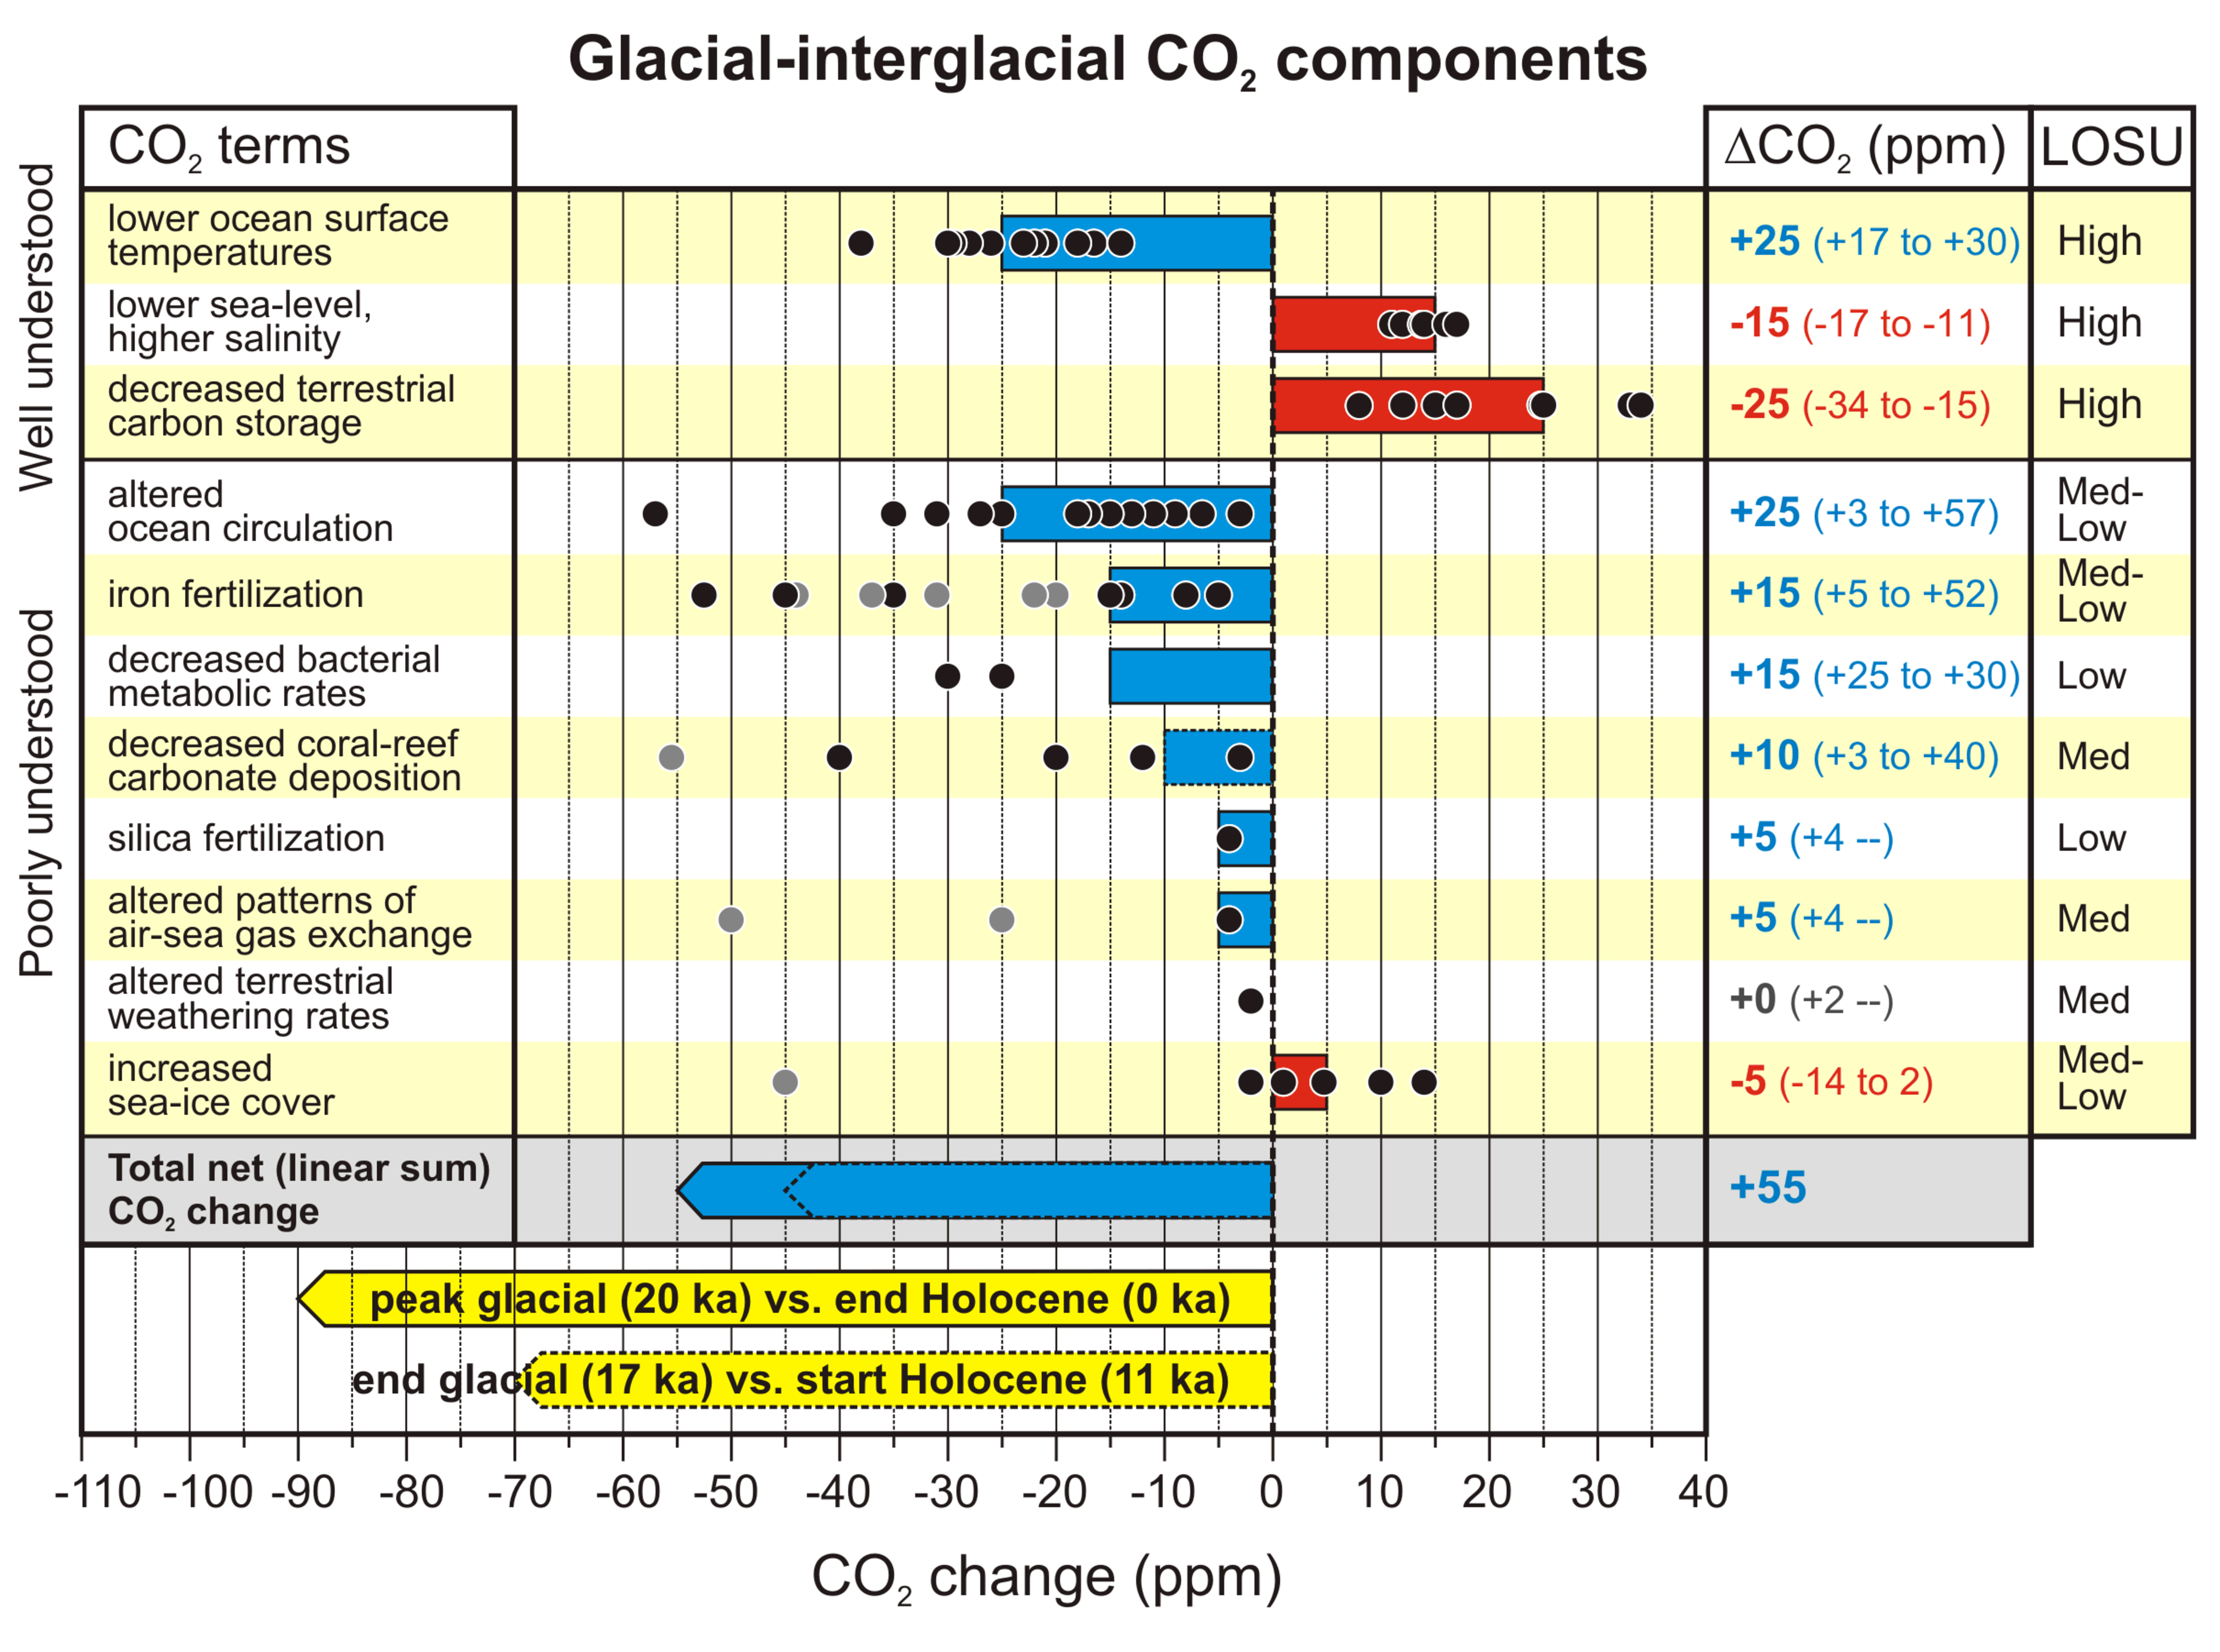
\includegraphics[width=1.00\textwidth]{CO2_components_110104.pdf}
\caption{Baaaa.}
\label{fig:CO2_components_110104}
\end{figure}

%----------------------------------------------------------------------------------------
%       CHAPTER X
%----------------------------------------------------------------------------------------

\cleardoublepage

\chapterimage{nSTnj.jpg} % Chapter heading image

\chapter{muffin model output}\label{ch:model-output}

\hfill \break

\vspace{24mm}

\noindent This section covers \textbf{muffin} saves data and how to ensure that the variables you want are saved and when you want.

\begin{itemize}
        \item Overview.
        \item \textit{Time-series} output.
        \begin{itemize}
                \item \textit{Time-series} file naming conventions.
                \item Specifying frequency and timing of \textit{time-series} data saving.
                \item Seasonal/monthly data saving.
        \end{itemize}
        \item \textit{Time-slice} output.
        \begin{itemize}
                \item \textit{Time-slice} file naming conventions.
                \item Specifying frequency and timing of \textit{time-slice} data saving.
        \end{itemize}
        \item Specifying which data fields to be saved in the \textit{time-series} and \textit{time-slice} format.
        \item \textit{Re-start} files.
\end{itemize}

%------------------------------------------------

\newpage

%------------------------------------------------

\section{Overview (and types of model output)}

The results of experiments are written to the directory: \textsf{\footnotesize \(\sim\)/cgenie\_output}

For any particular experiment, all saved model results, plus copies of input parameters and the model executable, are gathered together in a sub-directory of \textsf{\footnotesize \(\sim\)/cgenie\_output} that is assigned the same name as the experiment (== \textit{user-config} file name), e.g.: \textsf{\footnotesize EXAMPLE.worbe2.Ridgwelletal2007.SPIN}.

Every science module saves its results in its own individual sub-directory within the experiment directory. So for the module that calculates ocean biogeochemical cycles -- \textbf{BIOGEM}, the results files will thus be found in: \textsf{\footnotesize \(\sim\)/cgenie\_output/EXAMPLE.worbe2.Ridgwelletal2007.SPIN/biogem}

Note that the science module \textbf{ATCHEM} does not save its own results (\textbf{BIOGEM} instead saves relevant information about atmospheric composition and air-sea gas exchange) while \textbf{SEDGEM} essentially saves results \uline{only at the very end of a model experiment}\footnote{With the exception of sediment core location environmental properties, which are saved more frequently.}. (\textbf{BIOGEM} can also save the spatial distribution of sediment composition as \textit{time-slices} as well as mean composition as a time-series). Furthermore, in order to attain a common format for both ocean physical properties and biogeochemistry, \textbf{BIOGEM} saves a range of ocean physics properties in addition to temperature and salinity, such as: velocities, sea-ice extent, mixed layer depth, convective frequency, etc.

Saving full spatial distributions for any or all of the tracers at each and every time-step is not practical, not only in terms of data storage but also because of the detrimental effect that repeated disk access has on model performance. Instead, \textbf{BIOGEM} saves the full spatial distribution of whatever tracer, flux, and/or physical properties of the system are required (how what fields are required is specified is discussed later), only at one or more predefined time points (in years). These are called '\textit{time-slices}'. However, rather than taking an instantaneous snapshot, the time-slice is constructed as an average over a specified integration interval.

The second main data format for model output is that of a '\textit{time-series}' of change in a single (integrated) property of the Earth system. Model characteristics must be reducible to a single meaningful variable for this to be practical (i.e., saving the time-varying nature of 3-D ocean tracer distributions is not). Suitable metrics include: the total inventories in the ocean and/or atmosphere of various tracers (or equivalently, the mean global concentrations / partial pressures, respectively), global sea-ice coverage. Like \textit{time-slices}, the data values saved in the \textit{time-series} files represent averages over a specified integration interval (one year by default).

For both \textit{time-slices} and \textit{time-series} output, the files themselves are created during model initialization and are periodically updated (appended to) during the experiment. Hence, \uline{even before the experiment has finished they may contain data that is useful to view and can be used to check on the progress of an experiment}.

\subsubsection{ATCHEM}

\noindent In the \textbf{ATCHEM} results directory, only the following file will be present:

\begin{enumerate}

\vspace{1mm}\item \textsf{\footnotesize *\_restart.nc} -- \textit{Re-start} file -- a snap-shot of the 2D distribution of atmospheric composition at the very end of the experiment. Not intended for user-access, although it can be plotted just like any normal \textit{netCDF} format file.

\end{enumerate}\vspace{2mm}

\subsubsection{BIOGEM}

\noindent For \textbf{BIOGEM}, some or all of the following files will be present:

\begin{enumerate}

\vspace{1mm}\item \textsf{\footnotesize *\_restart.nc} -- \textit{Re-start} file -- a snap-shot of the 3D distribution of biogeochemical properties of the ocean at the very end of the experiment. Not intended for user-access, although it can be plotted just like any normal \textit{netCDF} format file.

\vspace{1mm}\item \textsf{\footnotesize fields\_biogem\_2d.nc} -- 2-D fields of (mostly) ocean bottom, ocean surface, and sediment surface properties.\footnote{The mid-points at which time-slices are saved are specified as described above.} Also: water-column integrals of certain geochemistry diagnostics, air-sea gas exchange fluxes, atmospheric composition (plus some physical atmospheric properties).

\vspace{1mm}\item \textsf{\footnotesize fields\_biogem\_3d.nc} -- 3-D fields of ocean dissolved and particulate tracer properties (plus some physical ocean properties).\footnote{The mid-points at which time-slices are saved are specified as described above.}

\vspace{1mm}\item \textsf{\footnotesize biogem\_series\_*.res}\footnote{\texttt{.res} is a useful format for processing in \textbf{MATLAB}; for other programs, other extensions are needed. If using the Mathematica data processing scripts - see \texttt{genie-docs/cGENIE.AutomationScripts} - \texttt{.dat} is needed; this can be set with  \texttt{gm\_string\_results\_ext=".dat"}} -- \textit{Time-series} results files -- globally and surface-averaged (and sometimes also benthic (bottom) surface averaged) property values as a function of time in plain text (ASCII) format.

\vspace{1mm}\item \textsf{\footnotesize biogem\_year\_*\_diag\_GLOBAL.res} -- Miscellaneous global diagnostic information. These files are saved at each requested \textit{time-slice} with the file-name string containing the mid-point of the time-slice (as years). The diagnostics include:
        \begin{itemize}
                \item time mid-point and integration interval
                \item global ocean surface area and volume
                \item mean global sir-sea gas exchange coefficient (for CO\begin{math}_2\end{math})
                \item mean atmospheric tracer concentrations plus total inventory
                \item mean ocean tracer concentrations plus total inventory
                \item mean plus total global productivity
                \item mean plus total global sedimentation
        \end{itemize}

\end{enumerate}\vspace{2mm}

\subsubsection{SEDGEM}

\noindent In the \textbf{SEDGEM} results directory, some or all of the following files will be written:

\begin{enumerate}

\vspace{1mm}\item \textsf{\footnotesize *\_restart.nc} -- \textit{Re-start} file -- a snap-shot of the 2D distribution of sedimentary properties at the very end of the experiment. Not intended for user-access, although it can be plotted just like any normal \textit{netCDF} format file.

\vspace{1mm}\item \textsf{\footnotesize fields\_sedgem\_2d.nc} -- Contains 2-D fields of sediment surface and ocean bottom properties.\footnote{This data is saved only at the termination of an experiment (i.e., the \textit{netCDF} file contains only a single time-slice).}

\vspace{1mm}\item \textsf{\footnotesize sedcore.nc} -- \textit{netCDF} format file containing the stacked records of accumulated deep-sea sediment composition.
\\The locations (if any) of sediment cores to be saved is specified in a plain text (ASCII) file pointed to by the string value of the \textit{namelist} parameter \texttt{sg\_par\_sedcore\_save\_mask\_name}\footnote{The location of this file is specified by the \textbf{SEDGEM} data input directory namelist parameter: \texttt{sg\_par\_indir\_name} which by default is \texttt{\~{}/genie-sedgem/data/input}.}. In the mask file, a '\texttt{1}' indicates a location to save a sediment core at, and a '\texttt{0}' indicates that no sediment core should be saved at this location.       This file must be present, so to save no sediment cores, simply populate the file with all zeros in an \texttt{xx} by \texttt{yy} grid.

\vspace{1mm}\item \textsf{\footnotesize sedcoreenv\_*} -- These files contain pseudo time-series of surface sediment environmental properties at each of the requested sediment core locations (if any are chosen).

\vspace{1mm}\item \textsf{\footnotesize seddiag\_misc\_DATA\_GLOBAL.res} -- A summary of mean global sedimentation, dissolution, and preservation fluxes, and surface sediment composition.

\vspace{1mm}\item \textsf{\footnotesize seddiag\_misc\_DATA\_FULL.res} -- Surface sediment and bottom water properties at each and every sediment grid point.

\end{enumerate}\vspace{2mm}

\subsubsection{ROKGEM}

\noindent In the \textbf{ROKGEM} results directory, some or all of the following files will be written:

\begin{enumerate}

\vspace{1mm}\item \textsf{\footnotesize fields\_rokgem\_2d.nc} -- 2-D fields of (mostly) land surface, ocean surface, and atmospheric properties related to weathering.

\vspace{1mm}\item \textsf{\footnotesize biogem\_series\_*} -- Time-series results files.

\end{enumerate}\vspace{2mm}

%------------------------------------------------

\newpage

%------------------------------------------------

\section{\textit{Time-slice} output}

%------------------------------------------------

\subsection{Frequency and timing of \textit{time-slice} data saving}

Rather than taking an instantaneous snapshot, the time-slice is averaged over a specified integration interval \begin{math}\Delta t\end{math} (in years), defined by the parameter: \texttt{bg\_par\_data\_save\_slice\_dt}\footnote{An empty list is valid - time-slices will then be populated for you at an interval set by the time-slice integration interval. But if you really don't want any time-slices, just set the first (or only) time point to occur beyond the end year of the run.}. The model state is thus integrated from time \begin{math}t_{n} - \Delta t/2\end{math} to \begin{math}t_{n} + \Delta t/2\end{math}. For instance, setting a value of \begin{math}\Delta t = 1.0\end{math} year results in all seasonal variability being removed from the saved time-slices, and successive time-slices then only reflect long-term (\textgreater 1 year) trends in system state.

\vspace{1mm}The mid-point years (\begin{math}t_{n}\end{math}) for which time-slices should be saved are specified in a single column pain text (ASCII) file in the \textsf{\footnotesize cgenie.muffin/genie-biogem/data/input} directory, whose name is specified by the parameter \textsf{\footnotesize bg\_par\_infile\_slice\_name}\footnote{The location of this file is specified by the \textbf{BIOGEM} data input directory parameter: \textsf{\footnotesize bg\_par\_indir\_name} which by default is \texttt{\~{}/genie-biogem/data/input}.}.
For example, the default \textit{time-slice} specification file \textsf{\footnotesize save\_timeslice.dat} contains the specification\footnote{The order in which the time sequence is ordered (i.e., ascending or descending time values) does not actually matter in practice as long as the list of times is ordered sequentially. The list will be internally re-ordered if necessary according to the selection of ‘BP’ (the model running backwards-in-time) or not according to the logical value of the parameter \texttt{bg\_ctrl\_misc\_t\_BP}, which is \texttt{.false.} by default.}:

\footnotesize\begin{verbatim}
-START-OF-DATA-
0.5
1.5
4.5
9.5
19.5
49.5
99.5
199.5
499.5
999.5
1999.5
4999.5
9999.5
19999.5
49999.5
99999.5
199999.5
499999.5
999999.5
-END-OF-DATA-
\end{verbatim}\normalsize
where \texttt{-START-OF-DATA-} and \texttt{-END-OF-DATA-} are simply tags delineating the start and end of the time point data.
Use of this particular specification lends itself to simple experiment run durations to be adopted (e.g., 10, 100, 10000 years). It provides a good generic starting point in that save frequency is faster to begin with (when environmental variables are more likely to be rapidly changing) and less frequently later (when environmental variables are unlikely to be changing rapidly and maybe converging to steady-state).

To change the time points used for \textit{time-slice} data saving, either direct edit this file (less good), or create a new file (e.g. simply copy and rename \textsf{\footnotesize save\_timeslice.dat}) with the required save frequency and timing and saved to the \textsf{\footnotesize cgenie.muffin/genie-biogem/data/input} directory, with the parameter \textsf{\footnotesize bg\_par\_infile\_slice\_name} pointing to the new filename).

%------------------------------------------------

\subsection{Saving at the experiment end}

Just in case an experiment run duration is chosen such that there is no corresponding save point anywhere near the end of the run, \uline{a \textit{time-slice} is automatically saved at the very end of an experiment} regardless of whether one has been specified or not and with the same averaging as used for the specified \textit{time-slices}.

This lend itself to a means of substantially reducing the amount of data saved, because if you specify no \textit{time-slices}, you will still end up with (just) the final year saved. You can make this happen (i.e. forcing only an end-of-run \textit{time-slice} to be saved), by adding to the \textit{user-config}:
\small\begin{verbatim}
# force time-slice save at run end only
bg_par_infile_slice_name='save_timeslice_NONE.dat'
\end{verbatim}\normalsize

%------------------------------------------------
%
\subsection{Seasonal/monthly data saving}

\textit{Time-slice} (but not currently \textit{time-series}) data can be saved seasonal or even monthly by selected by setting a single parameter rather than e.g. specifying a monthly or seasonal data save interval and editing the time-slice definition file with a series of min-points for months (or seasons).
The way it works is that the overall averaging interval (parameter: \texttt{bg\_par\_data\_save\_slice\_dt})\footnote{Default value = 999} is broken down into sub-intervals of averaging. i.e., breaking down a year interval (the default) into 4 will give seasonal averaging. The parameter: \texttt{bg\_par\_data\_save\_slice\_n} where \textit{n} sets the number of time steps in each sub-interval of data saving and hence determines whether the averaging is e.g. seasonal or monthly. The slightly tricky part is to be sure of how many time steps in each year ;)

By default, \textbf{\textit{c}GENIE.muffin} employs 96 time-steps per year for a 16-level ocean circulation model (\textbf{GOLDSTEIN}) and 48 for \textbf{BIOGEM}\footnote{Note that when running using \texttt{runmuffin.t100.sh}, 100 time-steps are taken in the ocean and 50 in BIOGEM for a 16 level ocean model.}. Hence for a 16-level ocean configuration, \uline{seasonal} data saving would be obtained with:
\begin{verbatim}bg_par_data_save_slice_n=12\end{verbatim}
(12 \textbf{BIOGEM} steps per averaging interval out of a total of 48), and \uline{monthly averages} with:
\begin{verbatim}bg_par_data_save_slice_n=4\end{verbatim}
(i.e. 4 \textbf{BIOGEM} steps for each of the 12 monthly averaging intervals, giving of a total of 48).

For lower resolution configurations of \textbf{\textit{c}GENIE.muffin}, \textbf{GOLDSTEIN} may be operating on 48 time-steps per year, and \textbf{BIOGEM} on 24 or even 12. As \textbf{\textit{c}GENIE.muffin} starts up it will report the ocean and biogeochemical time-stepping, such as:
\small\begin{verbatim}
>> Configuring ...
   Setting time-stepping [GOLDSTEIN, BIOGEM:GOLDSTEIN]:  100 2
\end{verbatim}\normalsize
which specifies 100 time-steps per year for \textbf{GOLDSTEIN}, and 50 per year (100/2) for \textbf{BIOGEM} for the case of a 16 level ocean using the \texttt{runmuffin.t100.sh} run script.
Note that for every year mid-point specified in the\textit{ time-slice} specification file, 4 or 12 (for seasonal and monthly, respectively) times as many time-slices will actually be saved.

%------------------------------------------------
%
\subsection{More frequent data saving}

Explicit frequent saving of fields or properties at specific locations can be done by setting a more higher save frequency of the time-slice data. However, because the 2D and 3D fields may contain a variety of unwanted variables in addition to the target one, save frequency is likely to be limited by the maximum \textbf{netCDF} file size that can sanely be manipulated, i.e. there is a limit to how large a file size you want to generate.

Several alternative options for cutting down the size of the saved data exist:

\vspace{1mm}
\begin{itemize}
\item (trivial) Make do with global or surface (or benthic) means in the \textit{time-series} output (rather than saving 2 or 3D data).
\item Cut down the types of data saved to the absolute minimum (see 'Data field selection' below).
\item Save only 2D data (rather than 2 \uline{and} 3D, which is the default). This can be accomplished by setting the parameters:
\vspace{-1mm}\begin{verbatim}
bg_ctrl_data_save_2d=.true.
bg_ctrl_data_save_3d=.false.
\end{verbatim}\vspace{-1mm}
(both are \texttt{.true.} by default). This disables the 3D data saving, although an empty 3D \textbf{netCDF} file will still be created.
\end{itemize}

\noindent One option to increase the frequency of 3D \textit{time-slice} data saving is to align it automatically with the frequency of \textit{time-series} data saving\footnote{This is in addition to normal 3D saving at the time-slice data saving frequency}. This can be done by setting:
\vspace{-1mm}\begin{verbatim}
bg_ctrl_data_save_3d_sig=.true.
\end{verbatim}\vspace{-1mm}
(by default, \texttt{.false.}).

\vspace{1mm}
\uline{The recommended/practical maximum for saved 3D \textit{time-slices} is around 100 (different \textit{time-slices})}, depending on the number of types of data field selected to be saved.

%------------------------------------------------
%
\subsection{Less(!) frequent data saving}

You could e.g. edit the default \textit{time-slice} specification file \textsf{\footnotesize save\_timeslice.dat}\footnote{(not recommended} or create your own with just a couple or even one single time-point. Or you can specify that no time-slice is saved(!) Actually, you will always get one -- at the very end of the model run.\footnote{A safety feature to ensure that however long the experiment runs, you always get data from the very end.} 

To do this (rather than creating a \textit{time-slice} specification file with a single entry equal to the last year of the intended model experiment), set:
\small\begin{verbatim}
# force time-slice save at run end only
bg_par_infile_slice_name='save_timeslice_NONE.dat'
\end{verbatim}\normalsize
(which points to an empty file).

%------------------------------------------------

\newpage

%------------------------------------------------

\section{\textit{Time-series} output}

%------------------------------------------------

\subsection{Frequency and timing of \textit{time-series} data saving}

For results \textit{time-series}, a file containing a series of model times (\begin{math}t_{n}\end{math}) at which data points need be saved is defined in the same way as for \textit{time-slices}, with the filename specified by the parameter \texttt{bg\_par\_infile\_sig\_name}. Again, the data values saved in the time-series file do not represent discrete values in time but an average, calculated from time \begin{math}t_{n} - \Delta t/2\end{math} to \begin{math}t_{n} + \Delta t/2\end{math} as per the construction of time-slices. The averaging interval, \begin{math}\Delta t\end{math}, is set by the value of the parameter \texttt{bg\_par\_data\_save\_sig\_dt}. The format is also identical to before (with tags delineating the start and end of the list of mid-points). If there are less than two elements present in the list, a default frequency of data saving will be invoked, set equal the averaging interval, except in the situation that this results in an unreasonably large amount of data, when an order of magnitude (or more than one order of magnitude where necessary) fewer save points are assumed.\footnote{For historical reasons ... the maximum number of time-series (and time-slice) data points was set to 4096. This is set by the parameter \texttt{n\_data\_max} in \texttt{biogem\_lib.f90} and can be altered if required.} 

\vspace{1mm}
The default setting:
\vspace{-1mm}
\small\begin{verbatim}bg_par_infile_sig_name='save_timeseries.dat'\end{verbatim}\normalsize
\vspace{-1mm}
provides for reasonably generic data saving, with the save frequency faster to begin with and becoming progressively less frequently later.

There is a related facility to \texttt{bg\_par\_infile\_sig\_name} for \textbf{SEDGEM} and \textbf{ROKGEM} in the parameter: \texttt{xx\_par\_output\_years\_file\_0d}, where \texttt{xx} is \texttt{sg} for \textbf{SEDGEM} and \texttt{rg} for \textbf{ROKGEM}. These specify files in the \textsf{\footnotesize genie-*gem/data/input} directory and again contain a list of years for 0D (time-series) output to be generated at. However, unlike \textbf{BIOGEM}, the data saved \textit{do} represent discrete values in time and \textit{not} e.g. annual averages.

%------------------------------------------------

\subsection{Saving orbital insolation}

[see orbits HOW-TO]

%------------------------------------------------

\newpage

%------------------------------------------------

\section{Data field selection}

Model output -- both \textit{time-slice} and \textit{time-series} data are saved in blocks or  by categories of model variables. For instance, all dissolved tracers in the ocean (3D netCDF \textit{time-slice} and/or \textit{time-series}), or all particle flux fields, all carbonate chemistry and associated variables, all surface sediment composition, etc etc. This still requires a multitude of parameters, one for each category and generally also one for each of \textit{time-slice} and \textit{time-series} data. In an attempt to simplify this, a single parameter, \texttt{bg\_par\_data\_save\_level}, specifying the sort and amount of data to save can be set instead.

The value of the \texttt{bg\_par\_data\_save\_level} save level parameter is given as an integer between \texttt{0} and \texttt{99}. The specific classes (groups) of data that are saved (as a mnemonic code) in response to each different selected save level are given in Table \ref{tab:timeslicelevels} (for \textit{time-slice} saving) and Table \ref{tab:timeserieslevels} (for \textit{time-series} saving), and what the mnemonics  strand for in terms of actual data saved (in real words), are defined in Tables \ref{tab:timeslicekey} and \ref{tab:timeserieskey}.

An alternative wordy summary to these tables would be: 

\vspace{1mm}
\begin{itemize}

\item[0] -- Save \textbf{nothing}.
\item[1] -- \textbf{Minimum} -- basic geochemistry only, i.e. ocean and atmosphere tracer fields (omitting e.g. the miscellaneous fields and time-series -- see below).
\item[2] -- \textbf{Basic} output == basic geochemistry and some physics.
\item[3] -- \textbf{Basic + biology} diagnostics, i.e. ocean and atmosphere tracer fields plus particulate  flux fields and biological diagnostics such as limitations on export.
\item[4] -- \textbf{Basic + geochemistry} diagnostics, including output on air-sea gas exchange, ocean carbonate chemistry, and geochemical diagnostics such as remineralization rates and transformation, ocean pH field (3D), Fe cycle and speciation diagnostics (2D). In conjunction with the \textbf{ROKGEM} module, also: weathering fluxes.\footnote{The most common option.} \item[5] -- \textbf{Basic + biology + geochemistry} diagnostics. A combination of \texttt{3} and \texttt{4}.
\item[6] -- \textbf{Basic + tracer + proxy} diagnostics. Tracer diagnostics includes: N*, P* etc., water column inventories (2D). Proxy diagnostics includes: ocean surface and benthic (and surface-benthic) tracers (2D). Also trace metals (e.g. C\(f\)d).\item[7] -- \textbf{Basic + biology + tracer + proxy} diagnostics.
\item[8] -- \textbf{Basic output + biology + tracer + proxy + geochemistry} diagnostics (a somewhat large selection of variables).
\item[9] -- \textbf{Basic output + full physics} (e.g. all grid specifications and properties).
\item[10] -- \textbf{Ocean acidification option} == biology and geochemical output fields plus all carbonate chemistry.
\item[11] -- \textbf{Preformed diagnostics option} == BASIC + biology + tracer + proxy + redox diagnostics.
\item[12] -- \textbf{Circulation option} == BASIC + tracer + physics diagnostics.
\item[14] -- \textbf{ BASIC + FULL (inc. redox) geochem} diagnostics.
\item[15] -- \textbf{ BASIC + biology + FULL (inc. redox) geochem} diagnostics.
\item[16] -- \textbf{ BASIC + biology + tracer + proxy + FULL (inc. redox) geochem} diagnostics.
\item[99] -- Save everything.
\item[>99] -- Use explicit user-specified settings for individual save categories. This is the default and is broadly consistent with previous version of the model.

\end{itemize}

\newpage

\noindent All of options \texttt{2-99} save as \textit{time-slices}:
\begin{itemize}[noitemsep]
\setlength{\itemindent}{.2in}
\item atmosphere tracer fields (2D)
\item ocean tracer fields (3D)
\item various miscellaneous diagnostics, including: ocean velocity (3D), overturning stream-function (2D), sea-ice extent and thickness (2D), incident radiation (2D), convection diagnostics (2D), air-sea gas exchange diagnostics (2D).
\item core-top sediment composition fields (2D) (if \textbf{SEDGEM} is selected)
\end{itemize}
and as \textit{time-series}:
\begin{itemize}[noitemsep]
\setlength{\itemindent}{.2in}
\item atmosphere tracer properties (as: atmospheric inventory (in \(mol\)) and concentration (\(mol\:kg^{-1})\) or isotopic composition)
\item ocean tracer properties (as: ocean inventory, plus mean (whole) ocean, or isotopic composition)
\item mean surface and benthic tracer properties
\item various miscellaneous diagnostics, including: insolation, sea-ice extent, volume, and thickness; global overturning stream-function, ocean surface pH, land surface temperature, and Fe parameters.
\item sediment (core-top) composition data (if \textbf{SEDGEM} is selected)
\end{itemize}

In addition, further output will be automatically added to the suite of saved data depending on the module selected and also for certain sorts of \textit{forcing}.

%------------------------------------------------

\newpage

%------------------------------------------------

\section{Re-start files}

\textit{Re-start} files are saved in the results directories of each module.
For \textbf{ATCHEM}, \textbf{BIOGEM}, and \textbf{SEDGEM}, these are in \textit{netCDF} format.

For the climate modules of \textbf{\textit{c}GENIE.muffin} (\textbf{GOLDSTEIN}, \textbf{GOLDSTEIN-SEAICE}, \textbf{EMBM}), \textit{re-start} files can be selected to farmermingo72be saved in either plain text (ASCII) or \textit{netCDF} format. ASCII format is the current default.

%------------------------------------------------

\newpage

%------------------------------------------------

\section{Useful output}

What follows is a short summary of some of the output and how it can be used.

Note -- depending on the specific model configuration (which model modules are selected) and selected tracers, as well as specific output choice, not all these variables and files will be present in the model output.

%------------------------------------------------

\subsection{Physics}

\begin{table}[ht]
\begin{tabular}{p{0.2\linewidth} p{0.317\linewidth} p{0.4\linewidth}}
\toprule
\textbf{Filename} & \textbf{Data} & \textbf{Application}\\
\textsf{\footnotesize biogem\_series\_*.res} & &\\
\midrule
\textsf{\footnotesize atm\_humidity} & \small{Mean surface humidity. (?)} & \small{(rarely used)}\\
\textsf{\footnotesize atm\_temp} & \small{Mean surface temperature. (degrees C)} & \small{Climate and climate change, when a simple global diagnostic is needed.}\\

\midrule

\textsf{\footnotesize misc\_opsi} & \small{Global minimum (-ve) and maximum (+ve) overturning stream-function, also reported for Atlantic and Pacific basins. Units of  Sv. (For certain modern configurations.)} & \small{Simple diagnostic of large-scale ocean circulation. There is some relationship of the maximum (negative and positive) overturning to ocean ventilation.}\\
\textsf{\footnotesize misc\_seaice} & \small{Sea-ice fractional cover (\textbackslash\%), thickness (m), and volume (m3).} & \small{As a simple climate (change) diagnostic.}\\
\textsf{\footnotesize misc\_SLT} & \small{Mean global surface land temperature. (C)} & \small{For calibrating and analysing global weathering rates.}\\
\textsf{\footnotesize ocn\_sal} & \small{Mean global, and typically also surface and benthic, ocean salinity. (PSU)} & \small{For characterizing freshwater changes and salinity \textit{forcing} impacts.}\\
\textsf{\footnotesize ocn\_temp} & \small{Mean global, and typically also surface and benthic, ocean temperature. (degrees C)} & \small{Climate and climate change. }\\

\bottomrule
\end{tabular}
\caption{Summary of the main (useful) \textit{time-series} output for climate-only ('physics') investigations.}
\end{table}

\begin{table}[ht]
\begin{tabular}{p{0.15\linewidth} p{0.20\linewidth} p{0.225\linewidth} p{0.325\linewidth}}
\toprule
\textbf{variable} & \textbf{variable} & \textbf{Description} & \textbf{Application}\\
 & (long name) & &\\
\midrule

\textsf{\footnotesize atm\_humidity} & \textsf{\footnotesize specific humidity} & \small{surface humidity (?)} & \small{(rarely used)}\\
\textsf{\footnotesize atm\_temp} & \textsf{\footnotesize surface air temperature"} & \small{surface air temperature (degrees C)} & \small{climate patterns and anomalies, comparison with terrestrial temperature proxies}\\
\midrule
\textsf{\footnotesize grid\_mask} & \textsf{\footnotesize land-sea mask} & \small{land-sea mask (n/a)} & \small{copy-paste-edit to create masks for data analysis}\\
\textsf{\footnotesize grid\_topo} & \textsf{\footnotesize ocean depth} & \small{ocean depth (m)} & \\

\midrule

\textsf{\footnotesize ocn\_sur\_sal} & \textsf{\footnotesize surface-water sal} & \small{surface ocean salinity (PSU)} & \small{diagnosing freshwater forcing impacts, regions of likely deep-water formation}\\
\textsf{\footnotesize ocn\_sur\_temp} & \textsf{\footnotesize surface-water temp} & \small{surface ocean temperature (degrees C)} & \small{diagnosing ocean circulation patterns, pole-to-equator temperature gradients, surface ocean temperature proxy comparisons}\\
\textsf{\footnotesize ocn\_ben\_temp} & \textsf{\footnotesize bottom-water temp} & \small{benthic temperature ( C)} & \small{diagnosing ocean circulation patterns, benthic temperature proxy comparisons}\\

\midrule

\textsf{\footnotesize phys\_cost} & \textsf{\footnotesize convective cost} & \small{rate of convective adjustments anywhere in the water column (n/a)} & \small{diagnosing deep mixed layers (and light limitation of biology) and deep-water formation regions}\\
\textsf{\footnotesize phys\_opsi} & \textsf{\footnotesize Global streamfunction} & \small{global overturning stream-function (Sv)} & \small{diagnosing large-scale ocean circulation patterns, sources of deep-water formation, deep ocean ventilation}\\
\textsf{\footnotesize phys\_psi} & \textsf{\footnotesize Barotropic streamfunction} & \small{barotropic stream-function (Sv)} & \small{diagnosing wind-driven ocean circulation patterns, effect of gateways}\\
\textsf{\footnotesize phys\_seaice} & \textsf{\footnotesize sea-ice cover (\%)} & \small{sea-ice cover (\%)} & \small{(climate / sea-ice)}\\
\textsf{\footnotesize phys\_seaice\_th} & \textsf{\footnotesize sea-ice thickness} & \small{sea-ice thickness (m)} & \small{(climate / sea-ice)}\\

\bottomrule
\end{tabular}
\caption{Summary of the main (useful, physics-focussed) 2D time-slice output.}
\end{table}

\begin{table}[ht]
\begin{tabular}{p{0.15\linewidth} p{0.20\linewidth} p{0.25\linewidth} p{0.3\linewidth}}
\toprule
\textbf{variable} & \textbf{variable} & \textbf{Description} & \textbf{Application}\\
 & (long name) & &\\
\midrule
\textsf{\footnotesize ocn\_sal} & \textsf{\footnotesize salinity} & \small{ocean salinity (PSU)} & \small{diagnosing ocean circulation patterns}\\
\textsf{\footnotesize ocn\_temp} & \textsf{\footnotesize temperature} & \small{ocean temperature (C)} & \small{diagnosing ocean circulation patterns}\\
\midrule
\textsf{\footnotesize phys\_u} & \textsf{\footnotesize ocean velocity - u} & \small{Eastwards component of ocean velocity (m/s)} & \small{diagnosing ocean circulation patterns and currents}\\
\textsf{\footnotesize phys\_v} & \textsf{\footnotesize ocean velocity - v} & \small{Northwards component of ocean velocity} (m/s) & \small{diagnosing ocean circulation patterns and currents}\\
\textsf{\footnotesize phys\_w} & \textsf{\footnotesize ocean velocity - w} & \small{upwards component of ocean velocity (m/s)} & \small{diagnosing ocean circulation patterns (note that velocity is measured at the top of an ocean depth layer, hence n/a for the surface layer)}\\
\bottomrule
\end{tabular}
\caption{Summary of the main (useful) 3D time-slice output.}
\end{table}

%------------------------------------------------
%
\clearpage
\subsection{(Bio)Geochemistry}

\begin{table}[ht]
\begin{tabular}{p{0.2\linewidth} p{0.317\linewidth} p{0.4\linewidth}}
\toprule
\textbf{Filename} & \textbf{Data} & \textbf{Application}\\
\textsf{\footnotesize biogem\_series\_*.res} & &\\
\midrule

\textsf{\footnotesize atm\_p\(CO_{2}\)} & \small{Global inventory (\(mol\)), mean concentration (\(atm\)) of atmospheric \(CO_{2}\). } & \small{Drivers of and feedbacks with climate. Diagnostic of response to carbon emissions (and removal).}\\
\textsf{\footnotesize atm\_p\(CO_{2}\)\_13C} & \small{\(^{13}C\) inventory (\(mol\)) and \(\delta^{13}C\) of atmospheric \(CO_{2}\).} & \small{Diagnostic of carbon emissions (and removal). Comparison with (terrestrial) proxy \(\delta^{13}C\) data.}\\
\textsf{\footnotesize atm\_pO2} & \small{Global inventory (\(mol\)), mean concentration (\(atm\)) of atmospheric \(O_{2}\). } & \small{ Limited use. Checking on \textit{restoring forcing} of atmospheric \(O_{2}\). Impacts of \(C_{org}\) burial if included in model.}\\

\midrule

\textsf{\footnotesize carb\_sur\_conc\_*} & \small{Carbonate chemistry components (mean surface) (\(molkg^{-1}\)).} & \small{Not generally useful. }\\
\textsf{\footnotesize carb\_sur\_H} & \small{Surface ocean mean \([H^{+}]\) (\(molkg^{-1}\)).} & \small{More useful is pH -- reported under \textsf{\footnotesize misc} (see below). }\\
\textsf{\footnotesize carb\_sur\_ohm\_arg} & \small{Mean surface aragonite saturation.} & \small{Ocean acidification impacts of \(CO_{2}\) release. Weathering impacts. Relates to carbonate production by (modern) corals, pteropods.}\\
\textsf{\footnotesize carb\_sur\_ohm\_arg} & \small{Mean surface calcite saturation.} & \small{Ocean acidification impacts of \(CO_{2}\) release. Weathering impacts. Carbonate production by foraminifera and coccolithophorids.}\\

\midrule

\textsf{\footnotesize diag\_misc\_} \hspace{1cm} \textsf{\footnotesize specified\_forcing\_*}  & \small{Applied flux \textit{forcings} (\(molyr^{-1}\)).} & \small{Whenever a \textit{restoring}, or \textit{flux} \textit{forcing} is specified, the actual flux employed, is saved here. Useful for diagnosing the flux associated with a restoring forcing (e.g. allowing  emissions flux associated with RCP (\textit{restoring forcing}) scenario to be diagnosed.)}\\

\midrule

\textsf{\footnotesize fexport\_CaCO3} & \small{Total flux (\(molyr^{-1}\)) and flux density (\(molm^{-2}yr^{-1}\)), of \(CaCO_{3}\) export from the ocean surface. } & \small{Carbonate production. Impacts of ocean acidification.}\\
\textsf{\footnotesize fexport\_POC} & \small{Total flux (\(molyr^{-1}\)) and flux density (\(molm^{-2}yr^{-1}\)), of \(POC\) export from the ocean surface. } & \small{Particulate organic matter export. Impacts of changes in nutrient supply and limitation.}\\

\midrule

\textsf{\footnotesize misc\_surpH} & \small{Mean surface \(pH\).} & \small{Ocean acidification.}\\

\midrule

\textsf{\footnotesize ocn\_DIC\_13C} & \small{Global inventory (\(mol\)), mean global,  surface, and  benthic \(\delta^{13}C\).} & \small{Carbon release and removal. Surface-benthic -- indicator or strength of carbon export and the biological pump, as well ocean ventilation.}\\
\textsf{\footnotesize ocn\_O2} & \small{Global inventory (\(mol\)), mean global,  surface, benthic concentrations (\(molkg^{-1}\)) of \(O_{2}\).} & \small{Indication of changes in ocean anoxia. (long-term) Imbalances between burial and weathering.}\\
\textsf{\footnotesize ocn\_PO4} & \small{Global inventory (\(mol\)), mean global,  surface,  benthic concentrations (\(molkg^{-1}\)) of \(PO_{4}\).} & \small{Nutrient limitation. (long-term) Imbalances between burial and weathering.}\\
\textsf{\footnotesize ocn\_TDFe} & \small{Global inventory (\(mol\)), mean global,  surface,  benthic concentrations (\(molkg^{-1}\)) of dissolved \(Fe\).} & \small{Nutrient limitation. (long-term) Imbalances between burial and weathering.}\\

\bottomrule
\end{tabular}
\caption{Summary of the main (useful, plus notes on a few less used) \textit{time-series} output for (bio)geochemistry (non ecological) investigations.}
\end{table}

\begin{table}[ht]
\begin{tabular}{p{0.15\linewidth} p{0.20\linewidth} p{0.225\linewidth} p{0.325\linewidth}}
\toprule
\textbf{variable} & \textbf{variable} & \textbf{Description} & \textbf{Application}\\
 & (long name) & &\\
\midrule

\textsf{\footnotesize atm\_*} & \textsf{\footnotesize } & \small{Distributions of gases and isotopes.} & \small{Not useful as the atmosphere is well-mixed. The \textit{time-series} outputs are simpler and more useful.}\\

\midrule

\textsf{\footnotesize carb\_ben\_ohm\_arg} \textsf{\footnotesize carb\_sur\_ohm\_cal} & \textsf{\footnotesize } & \small{Benthic aragonite and calcite saturation.} & Impacts of ocean acidification of distribution of benthic organisms. Indicator of sediment preservation.\\
\textsf{\footnotesize carb\_sur\_ohm\_arg} \textsf{\footnotesize carb\_sur\_ohm\_cal} & \textsf{\footnotesize } & \small{Ocean surface aragonite and calcite saturation.} & Impacts of ocean acidification of distribution of planktic organisms.\\

\midrule

\textsf{\footnotesize fseaair\_p\(CO_{2}\)} & \textsf{\footnotesize p\(CO_{2}\): net sea->air gas exchange flux density} & \small{Air-sea \(CO_{2}\) gas exchange.} & \small{Indicator of air-sea gas disequilibrium, regions of out-gassing/in-gassing.}\\

\midrule

\textsf{\footnotesize misc\_pH} & \textsf{\footnotesize ocean pH} & \small{Ocean surface pH.} & \small{Ocean acidification.}\\
\textsf{\footnotesize misc\_sur\_} \textsf{\footnotesize rCaCO3toPOC} & \textsf{\footnotesize CaCO3 to POC export rain ratio} & \small{Particulate \(CaCO_{3}:POC\) export ratio from ocean surface.} & \small{Ocean acidification impacts.}\\

\midrule

\textsf{\footnotesize ocn\_sur\_TDFe} & \textsf{\footnotesize surface-water TDFe} & \small{Ocean surface total dissolved \(Fe\) (\(molkg^{-1}\)).} & \small{Patterns of nutrient uptake and limitation.}\\
\textsf{\footnotesize ocn\_sur\_TDL} & \textsf{\footnotesize surface-water TDL} & \small{Surface   ligand concentrations (\(molkg^{-1}\)).} & \small{(Stabilizes dissolved Fe, but so not useful itself.)}\\
\textsf{\footnotesize ocn\_sur\_PO4} & \textsf{\footnotesize surface-water PO4} & \small{Ocean surface \([PO_{4}]\) (\(molkg^{-1}\)).} & \small{Patterns of nutrient uptake and limitation.}\\
\textsf{\footnotesize ocn\_ben\_PO4} & \textsf{\footnotesize bottom-water PO4} & \small{Benthic \([PO_{4}]\) (\(molkg^{-1}\)).} & \small{Indicator of large-scale ocean circulation and ventilation.}\\
\textsf{\footnotesize ocn\_ben\_DIC\_13C} & \textsf{\footnotesize } & \small{Benthic \(\delta^{13}C\).} & \small{Indicator of large-scale ocean circulation and ventilation. Model-data \(\delta^{13}C\) proxy comparison.}\\
\textsf{\footnotesize ocn\_int\_DIC} & \textsf{\footnotesize DIC water-column integrated tracer inventory} & \small{Pattern of water column integrated ocean \(DIC\) (i.e. dissolved carbon storage) (\(molm^{-2}\)).} & \small{Indicator of \(CO_{2}\) emissions storage and transport when used in difference/anomaly maps and calculations.}\\

\bottomrule
\end{tabular}
\caption{Summary of the main (mostly useful) 2D time-slice output for (bio)geochemistry.}
\end{table}


%------------------------------------------------

\clearpage
\subsection{Biology/Ecology}


%----------------------------------------------------------------------------------------
%       CHAPTER X
%----------------------------------------------------------------------------------------

\cleardoublepage

\chapterimage{chx-plotting1.png} % Chapter heading image

\chapter{Introduction to model results analysis}\label{ch:results-analysis}

\hfill \break

\vspace{21mm}

\noindent The primary format for saving spatial (2- and 3-D) data is \textit{netCDF} (network Common Data Form). More information on the netCDF format and the libraries necessary to compile the model can be found \href{http://www.unidata.ucar.edu/software/netcdf}{here}.
The writing of netCDF follows roughly the \href{http://www.cgd.ucar.edu/cms/eaton/cf-metadata/index.html}{CF1.0 convention} (NetCDF Climate and Forecast (CF) Metadata Convention).
The netCDF output is written for  the \textbf{BIOGEM} and \textbf{SEDGEM} modules separately, and both modules have a flag that suppresses spatial data file saving in ASCII format, with netCDF format being the default.

Under unix/linux, netCDF files can be interrogated with: \texttt{\$ ncdump -h filename.nc} which will give you the header information of the file. The command is included in the netCDF library which has to be present to run the model anyway. It's useful to get the NCO software package helping to concatenate files or extract variables as shell command. A full list of available software to manipulate or graphically illustrate netCDF files can be found \href{http://www.unidata.ucar.edu/software/netcdf/software.html}{here}.

\vspace{4pt}
This Chapter covers how to visualize \textbf{muffin} output, with a particular emphasis on (netCDF) spatial data, via:

\vspace{2pt}
\begin{itemize}
\vspace{1pt}
\item \textbf{Panoply}
\\ If you really really must insist on using Windozzzz, the recommended viewer for netCDF is \href{http://www.giss.nasa.gov/tools/panoply/}{Panoply} (see below). \textbf{Panoply} can be run under linux and on the Mac (OS X).
\\ There is also \href{http://www.epic.noaa.gov/java/ncBrowse/}{ncBrowse}. Again, this will also run under LINUX and on the Mac (OS X).
\vspace{1pt}
\item \textbf{MUTLAB}
\\ You can also view netCDF files using \textbf{MUTLAB}, for which a number of plotting functions are provided. An advantage here is that the \textbf{MUTLAB} code can be hacked to produce much more powerful and bespoke analysis and plots.
\end{itemize}

%------------------------------------------------

\newpage

%------------------------------------------------

\section{Plotting with Excel}

Just ... don't do it!\footnote{Obviously, there may be circumstances where it might be helpful to plot time-series output in \textbf{Excel}, although in practice, time-series output is much easier and faster to load in and plot with \textbf{MATLAB}.}

%------------------------------------------------

\newpage

%------------------------------------------------

\section{Plotting with Panoply}

In the following sub-sections are some pointers and examples of \textbf{Panoply} plotting.\footnote{*WARNING* These instructions are strictly valid for older version of \textbf{Panoply} (ca. version 2.9.4), although some updates to the text have been made in light of version 4.6.2 ... so be aware that the plotting control buttons and options may have subtly changed in newer versions and the text no longer reflect the exact (current) options in \textbf{Panoply} ...}

When you open a netCDF file, you will be presented with a \footnotesize\textsf{Datasets }\normalsize window (on the left hand side of the application window). This contains a list of all the variables available that you can display. You will find that the 'Long Name' description of the variable will be the most helpful to identify the one you want. Clicking (once) and highlighting an entry will display further information about that variable in the \footnotesize\textsf{Variable }\normalsize window on the left hand side of the application window.

In a drop-down box at the bottom of the application window is an option for shortening the list of displayed variables in the netCDF file:

\begin{itemize}[noitemsep]
\vspace{1mm}
\item \footnotesize\textsf{Georeferenced variables }\normalsize -- All the spatial (2 or 3D) variables.
\vspace{1mm}
\item \footnotesize\textsf{Plottable variables }\normalsize -- As above, but now including axis definitions (which can be plotted as 1D lines).
\vspace{1mm}
\item \footnotesize\textsf{All variables }\normalsize -- all of the variables.
\end{itemize}
\vspace{2mm}

To create a plot of a variable -- simply double-click anywhere on the line containing that variable. A dialogue box will open with various options (Figure \ref{fig:CreatePlot}). For 3-D model output, you have the option of whether you want a \footnotesize\textsf{'Lat-Vert'}\normalsize, \footnotesize\textsf{'Lon-Lat'}\normalsize, or \footnotesize\textsf{'Lon-Vert' }\normalsize plot (for the 2-D fields, the only choice is \footnotesize\textsf{'Lon-Lat'}\normalsize).
\begin{itemize}
\vspace{1mm}
\item \footnotesize\textsf{'Lat-Vert' }\normalsize plots -- a common way of visualizing vertical distribution in the ocean. The default is for \textbf{Panoply} to display an average of all longitudes in a zonal mean. Un-ticking the \footnotesize\textsf{Ave}\normalsize box in the \footnotesize\textsf{Array}\normalsize tab will enable you to specify a specific longitude section. Be aware that Panoply likes to plot the depth inverted by default ...
\vspace{1mm}
\item \footnotesize\textsf{'Lon-Lat' }\normalsize plots -- the classic 2D, top-down view of the ocean. There are multiple levels (depth layers) in the ocean of data that can be plotted, from the surface to the abyssal ocean.
\vspace{1mm}
\item \footnotesize\textsf{'Lon-Vert' }\normalsize plots -- (an uncommon option).
\end{itemize}
\vspace{2mm}
For all three: there may be multiple time-slices (i.e., you can plot data saved from different years).\footnote{Remember that the default, first time slice, will be the first once saved in the experiment. The last one saved and displayed, will reflect the end of your experiments.}

\begin{figure}[ht]
\begin{center}
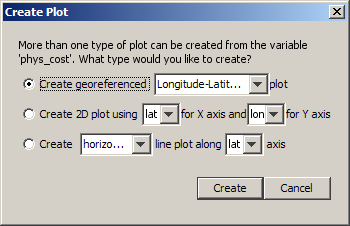
\includegraphics[scale=2.0]{CreatePlot.png}
\end{center}
\caption{\textbf{Panoply} \textsf{Create Plot} dialogue window.}
\label{fig:CreatePlot}
\end{figure}

You can interpolate the data or not (often you may find that it is clearer not to interpolate the data but to leave it as 'blocky' colors corresponding to the resolution of the model), change the scale and colors, overlay continental outline, change the projection, etc etc. Gray cells represent 'dry' grid points, i.e., continental or oceanic crust.
To save plots in \textbf{Panoply} -- from the file menu: \footnotesize\textsf{File}\normalsize, then \footnotesize\textsf{Save Image As ... }\normalsize and then select the location, filename, and graphics format.

%------------------------------------------------

\subsection{Issues with Panoply default settings}

The default settings in \textbf{Panoply}, i.e. those used when a plot is first created, can often mislead. In particular, note:
\begin{itemize}

\vspace{1mm}
\item \footnotesize\textsf{Year }\normalsize (\footnotesize\textsf{Array}\normalsize tab)
        \\ The default is for the very 1st \textit{time-slice} to be displayed rather than the experiment end. The first \textit{time-slice} is numbered from 1 to however many total time-slices have been saved (displayed to the immediate right of the \footnotesize\textsf{Year ,}\normalsize box), and it is this integer number that appears in the \footnotesize\textsf{Year }\normalsize box -- not the year of the data save. Instead, the mid-point year of the time-slice is displayed in a second box (labeled '\footnotesize\textsf{Year mid-point}\normalsize').
        \\ Different \textit{time-slices} to be plotted can be selected by either clicking through the saved year count, or by selecting the save year mid-point from the drop-down list.

\vspace{1mm}
\item \footnotesize\textsf{Scale Range }\normalsize (\footnotesize\textsf{Scale}\normalsize tab)
        \\ The color scale is auto-scaled so that the range always goes from the minimum to maximum displayed value. This can potentially mislead if save years and/or depth/latitude slices are scrolled through as the scale will be automatically adjusted to fit each plot in turn.
        \\ Confusion can also arise for fields with no variation, e.g. atmospheric trace gas concentrations or air temperature -- the auto-scaled plot in these instances has a uniform color but with odd hatching as Panoply dutifully tries to achieve the impossible (creating a scale of multiple colors for a single value).

\vspace{1mm}
\item Zonal averaging (\footnotesize\textsf{Array }\normalsize tab)
        \\ \footnotesize\textsf{Lat-Vert }\normalsize plots are displayed as a zonal mean by default. This is indicated by the tick in the \footnotesize\textsf{Ave }\normalsize box (bottom RH corner). Un-ticking the \footnotesize\textsf{Ave }\normalsize box releases the averaging with the first longitudinal value of the grid now displayed instead. Similar to how Panoply displays years -- the longitudinal grid locations are counter from 1 to typically 36 (depending on the resolution of the ocean grid), with the longitudinal mid-point value in degrees East displayed to the right.
        \\ Different longitudinal sections to be plotted can be selected by either clicking through the grid point number count, or by selecting the longitudinal mid-point from the drop-down list.

\vspace{1mm}
\item Scale bar tick marks (\footnotesize\textsf{Array }\normalsize tab)
        \\ The tick labels on the color scale are displayed by default in the format: \footnotesize\textsf{x.y }\normalsize. If the typical values of the variable are order e.g. 10\begin{math}^{-6}\end{math} you will end up with value labels ranging from \footnotesize\textsf{0.0 }\normalsize to \footnotesize\textsf{0.0 }\normalsize ... This can be most easily resolved in one of two ways:
        \begin{itemize}
\item The format of the label can be changed by selecting a different option from the pull-down \footnotesize\textsf{Tick Label Format }\normalsize box (default == \footnotesize\textsf{\%.1f}\normalsize). For instance, \footnotesize\textsf{\%.2e }\normalsize would give a display in the format \footnotesize\textsf{x.xxEyy }\normalsize (or \footnotesize\textsf{x.xxE-yy}\normalsize) or \footnotesize\textsf{\%.6f }\normalsize would give \footnotesize\textsf{x.xxxxxx}\normalsize.
\item An alternative is to re-scale the values. This is done in the Scaling Factor box in which you set the scale factor in powers of 10. For example: setting \footnotesize\textsf{-6}\normalsize in effect converts units of mol kg\begin{math}^{-6}\end{math} to \begin{math}\mu\end{math}mol kg\begin{math}^{-6}\end{math}.
\end{itemize}

\vspace{1mm}
\item Other things to watch out for include:
\begin{itemize}
\item A plot involving depth, being by default, 'up-side-down'!.
\\This is fixed in the \footnotesize\textsf{Grid}\normalsize tab, and the click button, \footnotesize\textsf{Swap B/T}\normalsize.
\item In \footnotesize\textsf{'Lon-Lat'}\normalsize plots, the modern continental outline being displayed by default.
\\This can be fixed by changing options in the \footnotesize\textsf{Overlay}\normalsize tab.
\end{itemize}

\end{itemize}
\vspace{2mm}

\begin{center}
\textbf{Simply be careful when opening a new plot that you are looking at what you *think* you are looking at (or what you think you are looking at *is* what you are looking at).}
\end{center}

Note that default plotting settings in \textbf{Panoply} can be changed (and saved).

%------------------------------------------------

\subsection{Basic plots -- examples}

\vspace{1mm}
\noindent\rule{4cm}{0.5pt}
\vspace{2mm}

\noindent\textcolor{red}{TO COME ...}

\vspace{1mm}
\noindent\rule{4cm}{0.5pt}
\vspace{2mm}

%------------------------------------------------

\subsection{Difference (anomaly) plots}

It is possible to create an anomaly (difference) maps in \textbf{Panoply} which are essential when analyzing changes in a variable that may be small compared to the global spatial variability. To do this:

\begin{itemize}
\vspace{1mm}
\item First, open the netCDF results file.
\vspace{1mm}
\item Open the variable of interest, e.g., \texttt{atm\_temp} (surface air temperature) in the 2D netCDF file.
\vspace{-4mm}
\item From the upper LH corner of the Dataset Browser window, from the drop-down menu, select the name of the plot you have just created (\texttt{atm\_temp} in \footnotesize\textsf{field\_biogem\_2D}\normalsize ...).
\vspace{1mm}
\item From the upper LH corner of the Dataset Browser window, now click on the \footnotesize\textsf{Combine Plot}\normalsize icon.
\\ You now have a plot window that is displaying a difference map. By default, it is showing you the difference between two identical (in time) slices. The two different slices are labeled Array 1 (LH side) and Array 2 (RH side).
\\NOTE: Easier than mucking about with \footnotesize\textsf{Combine Plot}\normalsize, is having open the first dataset, simply drag another variable from the list of variables in the \footnotesize\textsf{Sources }\normalsize window, into the \footnotesize\textsf{Plot }\normalsize window. You can drag either a different, or the same variable, into the \footnotesize\textsf{Plot }\normalsize window.
\end{itemize}
\vspace{2mm}

For instance, you can keep one array (Array 1) fixed to the initial (year 1 (centered on 0.5)) and vary the year in the second array (Array 2). Note that you can select in Panoply whether Array 1 - Array 2 is plotted, or Array 2 - Array 1, or various proportional or relative differences.

If you switch off the auto-scaling feature (\footnotesize\textsf{Always fit to data}\normalsize) you can center the scale so that no change is white, with positive deviations = red and negative = blue by clicking on Center on 0. This is something of a convention in the scientific literature.

The same variable in two different model experiments can also be opened up and analyzed combined:

\begin{itemize}
\vspace{1mm}
\item Start by opening up both required netCDF files.
\vspace{1mm}
\item Open the variable of interest in one (either one) of the two 2D netCDF data-sets.
\vspace{1mm}
\item From the upper LH corner of the Dataset Browser window, from the drop-down menu, select the name of the plot you have just created.
\vspace{1mm}
\item Now double-click in the variable in the 2nd netCDF dataset.
\\ You now have a plot window that is displaying a difference map, but of the same variable between two different experiments, rather than two years of the same experiment.
\end{itemize}
\vspace{2mm}

%------------------------------------------------

\subsection{Ocean velocity plots}

By combining the two (horizontal) fields of ocean circulation, rather than a difference plot, \textbf{Panoply} can create a velocity plot. This is a great way of visualizing surface (and deeper) currents and circulation patterns. To do this:

\begin{itemize}
\vspace{1mm}
\item First, open the 3-D netCDF results file.
\vspace{1mm}
\item Open either the \texttt{phys\_u} ('ocean velocity - u') or \texttt{phys\_v} ('ocean velocity - v') field and select a \footnotesize\textsf{Lon-Lat }\normalsize plot.
\vspace{1mm}
\item From the upper LH corner of the \footnotesize\textsf{Sources }\normalsize window, from the drop-down menu, select the name of the plot you have just created.
\vspace{1mm}
\item Now double-click on the other velocity variable (whichever of the u and v fields you did not open first).
\vspace{1mm}
\item By default you get a difference map, which is pretty useless really. From the drop-down \footnotesize\textsf{Plot }\normalsize menu box (which should be displaying 'Array 1 - Array 2' by default) select: \footnotesize\textsf{Vector Magnitude }\normalsize(bottom of the list).
\\ You now have a plot window that is displaying the ocean velocity field, with arrows indicating the direction and speed (length of the arrow) together with an interpolated color background of the speed.
\end{itemize}
\vspace{2mm}

You can re-scale the velocity arrows to more clearly display the circulation pattern by altering the \footnotesize\textsf{Scale Length }\normalsize value (\footnotesize\textsf{Contours \& Vectors }\normalsize tab). A value of 0.1 is a reasonable choice for surface currents. e.g. see Figure \ref{fig:cgenie_currents}.

If you want to display deeper (in the ocean) current fields and/or different time-slices, take care that the depth level (/time-slice) in both LH and RH sides of the \footnotesize\textsf{Array(s) }\normalsize panel must be changed to the same value. If displaying deeper current fields, then the velocity vectors will have to be further re-scaled (to a smaller value) in line with the lower velocities at depth compared to the surface.

\newpage

\begin{figure}[ht]
\begin{center}
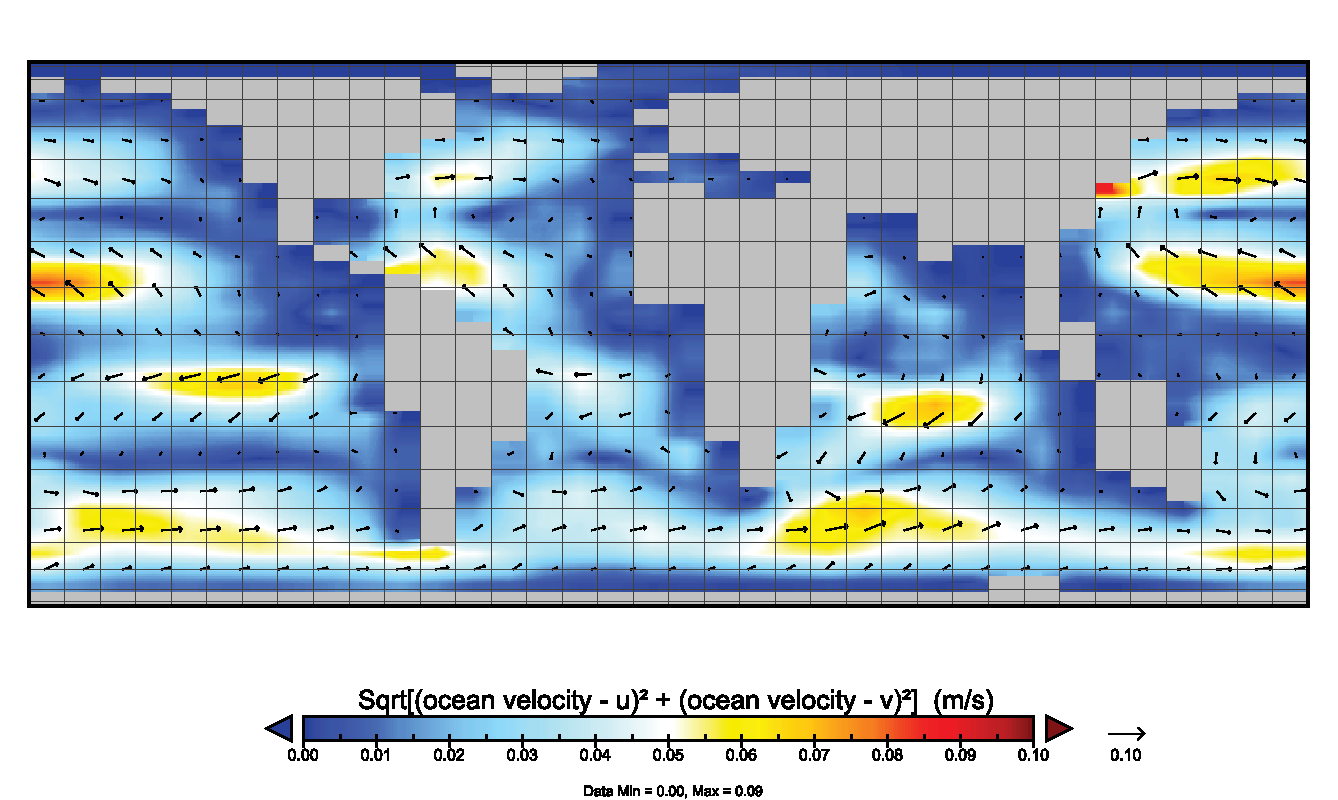
\includegraphics[scale=0.5]{cgenie_currents.pdf}
\end{center}
\caption{Example (modern) ocean surface velocity (current) map.}
\label{fig:cgenie_currents}
\end{figure}

%------------------------------------------------

\newpage

%------------------------------------------------

\section{MATLAB plotting}

%------------------------------------------------

\subsection{MATLAB 101}

If you need a tutorial on \textbf{MATLAB}, either as a refresher, or because you have not used the program before, refer to (and/or work through) the following sections of the \href{https://github.com/derpycode/matlabananas\#matlabananas}{matlabananas} \textbf{MATLAB} textbook:

\vspace{2pt}
\begin{itemize}
\vspace{1pt}
\item Chapter 1 --  this covers the very basics of using \textbf{MATLAB}, what variables are, including scalars (e.g. single numbers), vectors (1D array), matrices (2D array) and higher order arrays, now to index and carry out basic manipulation of arrays, basic data loading and saving and plotting.
\vspace{1pt}
\item Sections 2.1 and 2.2 of Chapter 2, which cover creating (script) programs -- i.e. adding all your \textbf{MATLAB} commands to a file (a \footnotesize\textsf{.m }\normalsize or '\footnotesize\textsf{m-file }\normalsize') and running the file, and \textit{functions} -- programs (\footnotesize\textsf{m-file}\normalsize s) where one or more parameters might be passed into the \textit{function} when it is called (e.g. at the command line), and potentially variables returned.
\vspace{1pt}
\item In Chapter 3 -- subsection 3.1.3 deals with reading in netCDF format data, which is the \textbf{muffin} format for spatial data. Section 3.2 deals with more advanced 2D plotting (also of direct relevance to \textbf{muffin} data processing and visualization using \textbf{MATLAB}).
\end{itemize}
\vspace{2pt}

%------------------------------------------------

\subsection{MATLAB and ASCII (\textit{time-series})}

The \textit{time-series} (\textsf{\footnotesize .res}) output of \textbf{BIOGEM} are in a simple plain text (ASCII) format. These can be read in very easily in \textbf{MATLAB} using the \texttt{load} command. Note that a brief description of each column of data in the \textit{time-series} files appears on the first first line of the file, and that prefixing this is a \texttt{\%} symbol, that \textbf{MATLAB} ignores. Hence only the columns of data gets read in by default using \texttt{load} :) \footnote{There are also other \textbf{MATLAB} commands for reading in text data -- refer to to the \href{http://www.seao2.info//teaching/201718.GEO111/GEO111.pdf}{\textbf{MATLAB} programming text}.} For example:

\small\begin{verbatim}
>> co2=load('biogem_series_atm_pCO_2.res','-ascii');
>> plot(co2(:,1),1.0E6*co2(:,3));
\end{verbatim}\normalsize

\noindent loads in the atmospheric \(CO_{2}\) time-series file (assigning it to the array variable \texttt{co2}), and then plots (as a line graph) the 3rd column (\(CO_{2}\) concentration) vs. the first (time). Because concentrations are saved in units of atmospheres, a factor of \texttt{1.0E6} is applied to concert to \(\mu atm\). Equivalently:

\small\begin{verbatim}
>> co2=load('biogem_series_atm_pCO2\).res','-ascii');
>> scatter(co2(:,1),1.0E6*co2(:,3));
\end{verbatim}\normalsize

%------------------------------------------------

\subsection{MATLAB 'Import Data' ...}

You can also import the time-series files by clicking on the \footnotesize\textsf{Import Data }\normalsize icon:

\begin{itemize}
\vspace{1pt}
\item Navigate to the \textbf{BIOGEM} sub-directory of your experiment results directory. Ensure that \footnotesize\textsf{All Files }\normalsize is selected and click on the time-series file you want.
\vspace{1pt}
\item \textbf{MATLAB} ignores the header lines, and it should be safe to simply click on \footnotesize\textsf{Import Selecftion }\normalsize for all columns, or select what you want to plot -- typically year (the first column) and another one.
\vspace{1pt}
\item A default variable name -- the filename minus the underscore characters -- will appear listed in the \textbf{MATLAB} \footnotesize\textsf{Workspace window }\normalsize. Double-click on the variable name to open up the imported data in a table view. If you select columns to plot, and then head over to the main \footnotesize\textsf{PLOTS }\normalsize tab, a range of plotting options are provided and a plot can be generated by clicking on one of the plotting icons.\footnote{Note that if you have not selected any data columns, then all the plotting icons are disabled and greyed out in the \footnotesize\textsf{PLOTS }\normalsize tab.}
\vspace{1pt}
\item Labels can be added, scales and markers changed, etc etc, in the \footnotesize\textsf{Figure window }\normalsize.
\end{itemize}
\vspace{2pt}

Note that as the data has been imported as an array in \textbf{MATLAB}, you can also plot directly from the command line. (And indeed, you could also have loaded the data from the command line.)

%------------------------------------------------

\subsection{MATLAB and netCDF (\textit{time-slice})}

\noindent Basically -- the only hard part, having opened the \textit{netCDF} file is in correctly deducing which dimension in an extracted data array is   longitude, latitude, (sometimes depth), or time. Mostly this should be pretty obvious from inspecting the \textbf{MATLAB} \footnotesize\textsf{Workspace }\normalsize window (assuming you have a column for \footnotesize\textsf{Size }\normalsize selected to be displayed), or using the \texttt{size} command.\footnote{It also turns out that the order of dimensions for a variable read in by \textbf{MATLAB}, is the opposite of the order listed in the \textsf{Variable} window of \textbf{Panoply}.} Once you have done this, you can plot slices, scale data, average or otherwise process data, extract locations at specific locations, etc etc.

As an example -- in \textbf{MATLAB}, first either change directory to the \textsf{\small biogem} directory of a set of \textbf{muffin} results, or from where-ever you are, add a path to the location of the \textsf{\small biogem} directory. To open the 2D \textbf{BIOGEM} netCDF results file, type:
\begin{verbatim}
>> ncid = netcdf.open('fields_biogem_2d.nc','nowrite');
\end{verbatim}

To extract a variable, you first need to find its ID from its name:
\begin{verbatim}
>> varid = netcdf.inqVarID(ncid,NAME);
\end{verbatim}
where \texttt{NAME} is a place-holder for the name of he variable (as a string). You might need to use \textbf{Panoply} to display all the different variable names. Or, you can list all the variables and stuff in the netCDF file using \texttt{ncdisp}:
\begin{verbatim}
>> ncdisp('fields_biogem_2d.nc')
\end{verbatim}

Having, by one means or another, identified the name of the variable you are interested in, you can recover its ID and then the data itself, for example, for \textsf{\footnotesize atm\_temp} (\textsf{\footnotesize surface air temperature}):
\begin{verbatim}
>> varid = netcdf.inqVarID(ncid,'atm_temp');
>> data  = netcdf.getVar(ncid,varid);
\end{verbatim}

In loading in the variable, you end up with a multi-dimensional array -- 2 spatial dimensions and if you have more than 1 \textit{time-slice} of data saved, 1 temporal dimension (and if you loaded in the \textbf{BIOGEM} 3D netCDF file, you end up with a 4-dimensional array). \textbf{MATLAB} reports the size of the array in the \textsf{\footnotesize Workspace window} (depending on which column display options you have selected). In the example here, which took the experiment \textsf{\footnotesize EXAMPLE.worjh2.Caoetal2009.RCP6p0}, the array for atmospheric temperature is reported as \(36\times36\times8\).\footnote{Although note that in \textbf{Panoply}, it is reported as \textsf{\scriptsize atm\_temp(time=8, lat=36, lon=36)}.} so the last of the 8 time-slices would  be accessed as:
\begin{verbatim}
>> data_last = data(:,:,8);
\end{verbatim}
or
\begin{verbatim}
>> data_last = data(:,:,end);
\end{verbatim}

Panoply reports variables in the the \textbf{BIOGEM} 3D netCDF file as having dimensions of: (\textit{time, zt, lat, lon}) (e.g. (time=13, zt=16, lat=36, lon=36)) whereas \textbf{MATLAB} reads it in the reverse order. For instance, if we load in the (3D) ocean temperature field:
\begin{verbatim}
>> ncid = netcdf.open('fields_biogem_3d.nc','nowrite')
>> varid = netcdf.inqVarID(ncid,'ocn_temp');
>> data  = netcdf.getVar(ncid,varid);
\end{verbatim}
and then type:
\begin{verbatim}
>> size(data)
ans =
    36    36    16    13
\end{verbatim}
we get an array orientated as (\textit{lon, lat, zt, time}).\footnote{\textit{zt} is the depth level in the ocean.} The final time-slice would hence then be accessed:
\begin{verbatim}
>> data_last = data(:,:,:,end);
\end{verbatim}
with \texttt{data\_last} now becoming a 3D array with dimensions (\textit{lon, lat, zt}).

\vspace{2mm}
There are three key things to remember at this point:

\begin{enumerate}
\setlength{\itemindent}{.2in}

\vspace{1mm}
\item Firstly, the depth levels are read such that index \texttt{1} is the surface, and \texttt{16} is the deepest ocean depth level (in this case, otherwise it is \texttt{8}).

\vspace{1mm}
\item For the lon-lat part -- (\textit{lon, lat}) equates to \textit{row}\textit{}s vs. \textit{columns} in \textbf{MATLAB}, and hence if you were to plot e.g. the surface ocean slice:
\begin{verbatim}
>> imagesc(data_last(:,:,1));
\end{verbatim}
you will end up with the plot on its side, with latitude along the \textit{x}-axis and longitude on the \textit{y}-axis.
\\You can exchange rows and columns in \textbf{MATLAB} with the \textit{transpose operator} (see programming/\textbf{MATLAB} book):
\begin{verbatim}
>> imagesc(data_last(:,:,1)');
\end{verbatim}
but ... this still leaves you with an up-side-down plot, because \textbf{MATLAB} reads from the first row down, whereas in latitude, you are expecting to read from -90 degrees up (towards the N pole). \texttt{flipud} accomplishes the final transformation:
\begin{verbatim}
>> imagesc(flipud(data_last(:,:,1)'));
\end{verbatim}

\vspace{1mm}
\item The final complication is that \textbf{muffin} netCDF output uses a special value to represent an invalid or null number, e.g. for ocean temperature where the grid point is land (and an ocean temperature value would have no meaning). In the netCDF definition, \textbf{Panoply} is told what the special number is, hence it shows land in grey when plotting ocean variables.

Panoply reports this as: \textsf{\footnotesize missing\_value = 9.969209968386869E36}.

\vspace{1mm}
There is no easy way (that I can see!) to get \textbf{MATLAB} to deal with this for you, so you need to search and replace this value, e.g.:
\small\begin{verbatim}
>> null=9.969209968386869E36;
>> data_last(find(data_last==null))=NaN;
\end{verbatim}\normalsize
which searches for this null value and replaces it with a \texttt{NaN} (so that now it can be simply plotted).

\end{enumerate}
\vspace{2mm}

Once you are done accessing data, it is good practice to close the netCDF file after you are done with it:
\begin{verbatim}
>> netcdf.close(ncid);
\end{verbatim}

The question then remains: what do you actually 'do' with it in \textbf{MATLAB}?

%------------------------------------------------

\subsubsection{Plotting sections}

For a quick look-see, \texttt{imagesc} (as per above) is handy.

\noindent For more advanced plotting (and for presentation) -- refer to the \textbf{matlabananas} \textbf{MATLAB} programming text.

\noindent As per above, horizontal (lon-lat) fields can be extracted from 2D \textit{netCDF} output by: \texttt{data(:,:,time)} and from 3D by: \texttt{data(:,:,zt,time)}. Obviously, you could also extract lon-depth via: \texttt{data(:,lat,:,time)} and lat-depth via: \texttt{data(lon,:,:,time)}.

\noindent Anomalies (with time) are created: \texttt{data(:,:,:,time2)-data(:,:,:,time2)}.

Typically, except a little trial-and-error in extracting the dimensions you want, and also in correcting the orientation of the matrix or resulting plot.

%------------------------------------------------

\subsubsection{Calculating inventories}

Often, the inventory (total mass or number of moles) of the ocean or atmosphere is useful to know, particularly as a function of time. For the ocean (or atmosphere) as a whole, the \textit{time-series} output files report this (alongside the mean global concentration).

You can also calculate this with \textbf{MATLAB} from the netCDF output. Fields of ocean concentration are saved in the 3D output (and atmospheric concentrations in the 2D output). To convert concentration in the ocean, in units of \(molkg^{-1}\) you'll need to know the mass of each ocean cell, in units of \(kg\).

When saving using save option \texttt{9}, or \texttt{99}\footnote{Parameter \texttt{bg\_par\_data\_save\_level} -- see earlier.}, you save the 'physics' of the ocean model, which is actually mostly just the grid information, such as cell area, thickness, latitude and longitude edges and midpoints, depth edges and mid point. Also saved are the masses and volumes of the grid of cells. So to derive an array of cell tracer inventories from an array of concentrations, and the array of cell masses (variable \textsf{\footnotesize phys\_ocn\_M}), you'd write:

\pagebreak

\small\begin{verbatim}
varid = netcdf.inqVarID(ncid,'ocn_temp');
data  = netcdf.getVar(ncid,varid);
varid = netcdf.inqVarID(ncid,'phys_ocn_M');
mass  = netcdf.getVar(ncid,varid);
inventory = data(:,:,:,time).*mass(:,:,:,time);
\end{verbatim}\normalsize
\noindent Before summing \texttt{inventory} to determine the global total inventory, you will, as before, have to deal with the null values (converting them to \texttt{NaN}) and then deal with the presence of \texttt{NaN}s in the array when summing ...

The advantage of doing the calculations in \textbf{MATLAB} (despite being provided with the global mean and inventory in the time-series files) is that you could calculate the inventory of a tracer (/substance) for just the ocean surface, or just a specific region of band of latitude. Or you could calculate the mean concentration for just a specific region of the ocean.\footnote{In calculating mean concentrations, you'll need to volume or mass weight the concentrations, and hence still need to use one of the physics variables.}

%----------------------------------------------------------------------------------------
%       CHAPTER X
%----------------------------------------------------------------------------------------

\cleardoublepage

\chapterimage{chx-plotting.png} % Chapter heading image

\chapter{muffinplot}\label{ch:muffinplot}

\hfill \break

\vspace{18mm}

\noindent The \textbf{muffinplot} suite of \textbf{MATLAB} functions provides a means of plotting a variety of output reproducibly (by means of  a saved parameter file) and with the potential for automation (i.e. automatically generating the same analysis for a large number of different experiments).

The functions comprising this software suite include:

\begin{itemize}[noitemsep]
\vspace{1mm}
\item \footnotesize\textsf{plot\_fields\_biogem\_2d}\normalsize -- lon-lat plots from the 2D \textbf{biogem} output.
\vspace{1mm}
\item \footnotesize\textsf{plot\_fields\_biogem\_3d\_i}\normalsize -- lat-depth plots from the 3D \textbf{biogem} output.
\vspace{1mm}
\item \footnotesize\textsf{plot\_fields\_biogem\_3d\_k}\normalsize -- lon-lat plots from the 3D \textbf{biogem} output.
\vspace{1mm}
\item \footnotesize\textsf{plot\_fields\_ccd}\normalsize -- analsysis of the 'CCD' (from both \textbf{biogem} 2D and \textbf{sedgem} 2D output).
\vspace{1mm}
\item \footnotesize\textsf{plot\_fields\_sedgem\_2d}\normalsize -- lon-lat plots from the 2D \textbf{sedgem} output.
\vspace{1mm}
\item \footnotesize\textsf{plot\_histc\_2d}\normalsize -- a generic color-coded histogram function.
\vspace{1mm}
\item \footnotesize\textsf{plot\_sedcore}\normalsize -- down-core plots from \textbf{sedgem} sedcore output.
\vspace{1mm}
\item \footnotesize\textsf{plot\_timeseries\_biogem}\normalsize -- time-series plots from \textbf{biogem} time-series output.
\end{itemize}
Note that at this current time, there is no facility for lon-depth plotting (unlike in \textbf{Panoply}).

Most of the plots also perform additional functions (which can be generally disabled if not wanted), such as plotting and saving zonal or depth profiles, plotting difference maps, plotting and labelling data on maps and carrying out model-data fit statistics and plotting, extracting model values at data locations.

The following sections provide an overview and examples of such plotting and analysis.

%------------------------------------------------

\section{Installation}

\textbf{muffinplot} can be obtained from \href{https://github.com/derpycode/muffinplot\#https://github.com/derpycode/muffinplot}{github}. If you do not have a \textbf{git} client on your computer (and hence cannot clone the repository locally), then simply download the archive file of all the code (from \footnotesize\textsf{\textcolor[rgb]{0,0.501961,0}{clone or download }}\normalsize -- pick \textsf{\footnotesize Download ZIP}).

When you unpack (or clone) \textbf{muffinplot} (note that it is likely to unpack by default into its own directory), you should see 3 directories -- \footnotesize\textsf{EXAMPLES}\normalsize, and \footnotesize\textsf{MASKS}\normalsize,\ \footnotesize\textsf{source}\normalsize, a series of \footnotesize\textsf{.m }\normalsize files, and a single lonely \footnotesize\textsf{.ps }\normalsize graphics file (\footnotesize\textsf{colorscales.ps}\normalsize). The \footnotesize\textsf{.m }\normalsize files are split into filenames with or without the label \footnotesize\textsf{SETTINGS }\normalsize -- the ones without are code files (\textit{functions}), and the ones with the word \footnotesize\textsf{SETTINGS }\normalsize in their filename, contain parameter settings for plotting.

By default (the parameters can be changed if you wish), wherever you run the \textbf{muffinplot} plotting function from, requires that you also have a subdirectory called \footnotesize\textsf{cgenie\_output}\normalsize\ present, and that the (complete) \textbf{muffin} experiment output directories of anything you want to plot should be in subdirectories of that -- i.e. the contents of \footnotesize\textsf{cgenie\_output }\normalsize should look like the contents of \footnotesize\textsf{cgenie\_output }\normalsize on your cluster account\footnote{Although you do not need to copy \uline{all} the results over ... just the experiments that you wish to plot up.}. Mask files reside in the \footnotesize\textsf{MASKS}\normalsize\ subdirectory of the \textbf{muffinplot} installation, or in your current directory, or anywhere in the \textbf{MATLAB} path.

The simplest option is to unpack/clone \textbf{muffinplot} to a directory containing \footnotesize\textsf{cgenie\_output }\normalsize and hence all your experimental results directories.\footnote{However, the \textbf{muffinplot} functions do not have to be run from the same directory that you are in -- you can install them somewhere convenient, and then with \textbf{MATLAB} set to a directory containing a \textsf{cgenie\_output} experiment results directory, you can:
\\\texttt{>> addpath(PATH)}
\\where \texttt{PATH} is the path to the directory where \textbf{muffinplot} is installed.}
In other words:
\begin{enumerate}[noitemsep]
\vspace{1mm}
\item Create some local directory e.g. called \footnotesize\textsf{RESULTS}\normalsize.
\vspace{1mm}
\item Create a subdirectory in \footnotesize\textsf{RESULTS }\normalsize called \footnotesize\textsf{cgenie\_output}\normalsize.
\vspace{1mm}
\item Drag your experiment results folders across into the subdirectory \footnotesize\textsf{cgenie\_output}\normalsize, as per the directory structure on the cluster. (Or better -- drag the archived files to  \footnotesize\textsf{cgenie\_output }\normalsize and unpack them.)
\vspace{1mm}
\item Install \textbf{muffinplot} in the \footnotesize\textsf{RESULTS }\normalsize directory.
\vspace{1mm}
\item Change the \textbf{MATLAB} working directory to \footnotesize\textsf{RESULTS}\normalsize.
\end{enumerate}
\vspace{2mm}

The plotting functions are run simply by typing their name and passing a list of parameters (comma-separated, with the complete list enclosed in parentheses). By default,   the \footnotesize\textsf{SETTINGS }\normalsize files need to be in the same directory as you are running the functions from, or in one of the \textbf{MATLAB} paths. Results are saved to a subdirectory that by default is called \footnotesize\textsf{PLOTS}\normalsize, which will be created for you if it does not already exist.

All the plotting functions provide some manner of 'help', that can be obtained by typing at the command line:
\vspace{-2pt}\begin{verbatim}
>> help FUNCTIONNAME
\end{verbatim}\vspace{-2pt}
where \texttt{FUNCTIONNAME} is the function name (as per listed above).

%------------------------------------------------

\newpage 
\section{Time-series plotting}

The \textbf{muffinplot} function \textsf{\footnotesize plot\_timeseries\_biogem.m} provides a facility to plot \textbf{BIOGEM} \textit{time-series} (\textsf{\small .res}) output.\footnote{Obviously -- there are lots of different and easy ways of plotting plain text output in the form of a simple column format.} You can use \textbf{MATLAB} \texttt{help} on the function name to detail the parameters that need to be passed (and examples).

The \textsf{\footnotesize plot\_timeseries\_biogem} plotting function plots a basic set of time-series variables by default. It then, enables a set up up to 3 additional variables to be plotted. It is also associated with a file of parameter values (\textsf{\footnotesize plot\_timeseries\_SETTINGS.m} by default) for fine-tuning plots.

The plotting function requires a list of parameters to be passed in the argument list, i.e.:
\begin{verbatim}
>> plot_timeseries_biogem(PAR1,PAR2,PAR3, ... PARn)
\end{verbatim}

These are, in order:

\vspace{1mm}
\begin{enumerate}
\item \texttt{PEXP1} -- \textit{string} \(\rightarrow\) the (first) experiment name.
\item \texttt{PEXP2} -- \textit{string} \(\rightarrow\)  is the name of the 2nd (optional) experiment. If no second experiment is selected, then a null string value must be passed, i.e., \texttt{''}.
\item \texttt{PTMIN} -- \textit{real} \(\rightarrow\) minimum plotted time (\textit{x}-axis).
\item \texttt{PTMAX} -- \textit{real} \(\rightarrow\) maximum plotted time (\textit{x}-axis).
\item \texttt{PDATA1} -- \textit{string} \(\rightarrow\) time-series variable name for additional data to plot.
\\Omit the '\texttt{biogem\_series\_}' and '\texttt{.res}' parts of the filename.
\\Leave blank, i.e., '', for no additional data panel.
\item \texttt{PDATA1N} -- \textit{integer} \(\rightarrow\) the column number of the data in the time-series file.
\item \texttt{PDATA2} -- \textit{string} \(\rightarrow\) time-series variable name for additional data to plot.
\item \texttt{PDATA2N} -- \textit{integer} \(\rightarrow\) the column number of the data in the time-series file.
\item \texttt{PDATA3} -- \textit{string} \(\rightarrow\) time-series variable name for additional data to plot.
\item \texttt{PDATA3N} -- \textit{integer} \(\rightarrow\) the column number of the data in the time-series file.
\item \texttt{POPT} -- \textit{string}\(\rightarrow\) The string for an alternative plotting parameter set.
\\If an empty\texttt{ ('') }value is passed as this parameter, then the default parameter set file is used.
\item \texttt{PNAME}  -- \textit{string}\(\rightarrow\) The string for an alternative filename.
\end{enumerate}
\vspace{2mm}
Note that if an empty value is passed as this parameter, then a filename is automatically generated.

A simple example usage would be:

\begin{verbatim}
>> plot_timeseries_biogem('myexperiment','',0.0,10000.0,'',0,'',0,'',0,'','')
\end{verbatim}
where \texttt{myexperiment} is the name of the 1st experiment, followed by and empty string (\texttt{''}) indicating no second experiment. The results are to be plotted from 0.0 to 10000.0 years (the 2 following parameters; \texttt{0.0,10000.0}). Then, no additional (maximum 3) optional parameters are requested, and hence the next parameters passed are: \texttt{'',0,'',0,'',0}. Finally, the default plotting parameter set is required, and no specific alternative filename is ot be used, accounting for the final 2 empty strings passed.

By default, \textsf{\footnotesize plot\_timeseries\_biogem} plots 2 panels of data, both with 2 (LH\ and RH) axes:

\begin{enumerate}[noitemsep]
\vspace{1mm}
\item Atmospheric \(CO_{2}\). Note that if the experiment was not \(CO_{2}\)-enabled (i.e. not run with a global carbon cycle), a warning is given and 'fake' data (actually, random numbers) is plotted.
\vspace{1mm}
\item Atmospheric \(\delta ^{13}CO_{2}\). Note that if the experiment was not \(\delta ^{13}CO_{2}\)-enabled (i.e. not run with a global carbon cycle), a warning is given and 'fake' data is plotted.
\vspace{1mm}
\item Atmospheric temperature (as a global mean, annual average).
\vspace{1mm}
\item Fractional (percentage) sea-ice extent.
\end{enumerate}
\vspace{2mm}

Additional model outputs can then be added by listing them in the function call. For example, to also plot the global overturning strength, which is contained in the file \footnotesize\textsf{biogem\_series\_misc\_opsi.res}\normalsize, you would add \texttt{'misc\_opsi',3}\footnote{Don't forget that you omit the '\texttt{biogem\_series\_}' and '\texttt{.res}' parts of the filename.}, where the \texttt{3} indicates the 3rd column of data in the file is to be plotted, which in this case is the global maximum overturning value (and the 2nd column is the minimum value). The complete line looks like:
\small\begin{verbatim}
>> plot_timeseries_biogem('myexperiment','',0.0,10000.0,'misc_opsi',3,'',0,'',0,'','')
\end{verbatim}\normalsize

By default, the plotted variables are all auto-scaled. To specify the y-axes, you will need to edit the plotting settings parameter file: \footnotesize\textsf{plot\_timeseries\_SETTINGS.m}\normalsize. For the default plotted 4 results variables, the minimum and maximum y-axis limits are specified in the section:
\vspace{1mm}
\begin{itemize}
\item[] \texttt{axis\_pCO2min = 0.0;}
\item[] \texttt{axis\_pCO2max = 0.0;}
\item[] \texttt{axis\_d13Cmin = 0.0;}
\item[] \texttt{axis\_d13Cmin = 0.0;}
\item[] \texttt{axis\_Tatmmin = 0.0;}
\item[] \texttt{axis\_Tatmmin = 0.0;}
\item[] \texttt{axis\_icemin = 0.0;}
\item[] \texttt{axis\_icemin = 0.0;}
\end{itemize}
\vspace{2mm}
The default zero values here, tell the plotting function to create an auto-scale for the y-axis.\footnote{Note the units of atmospheric \(CO_{2}\) as \(\mu atm\).} Following this in the parameter file, are the settings for the optional variable plotting:
\vspace{1mm}
\begin{itemize}
\item[] \texttt{axis\_data1\_min = 0.0;}
\item[] \texttt{axis\_data1\_max = 0.0;}
\item[] \texttt{axis\_data2\_min = 0.0;}
\item[] \texttt{axis\_data2\_max = 0.0;}
\item[] \texttt{axis\_data2\_min = 0.0;}
\item[] \texttt{axis\_data2\_max = 0.0;}
\end{itemize}
\vspace{2mm}

Note that if you want instead to copy and rename and then edit this settings file, you will need to pass the new (non-default) filename when calling the plotting function. For example, if you created a new parameter settings file: \footnotesize\textsf{settings\_NEW.m }\normalsize, then the \textit{function} call would look like:
\small\begin{verbatim}
>> plot_timeseries_biogem('myexperiment','',0.0,10000.0,'',0,'',0,'',0,'settings_NEW','')
\end{verbatim}\normalsize

%------------------------------------------------

\section{Spatial plotting}

%------------------------------------------------

\subsubsection{Overview}

4 of the \textbf{muffinplot} plotting functions provide spatial (2D) plotting capabilities:
\vspace{2mm}
\begin{itemize}

\item \texttt{plot\_fields\_biogem\_2d}
\\Plot a 2-D field from: \footnotesize\textsf{fields\_biogem\_2d.nc}\normalsize.

\item \texttt{plot\_fields\_biogem\_3d\_i}
\\Plot a vertical-meridional (2-D) slice through the ocean (i.e., all cells have the same \texttt{i} (longitudinal) coordinate value) from: \footnotesize\textsf{fields\_biogem\_3d.nc}\normalsize.
\\Options are  provided for averaging longitudinally over a supplied mask, which may be the entire ocean and hence giving a global meridional cross-sectional mean, of a specific ocean basin, or may be a single cell 'wide' longitudinally and take a meandering path hence simulating an ocean transect. An option is also provided to overlay an ocean circulation stream-function.

\item \texttt{plot\_fields\_biogem\_3d\_k.m}
\\Plot a horizontal slice through the ocean from: \footnotesize\textsf{fields\_biogem\_3d.nc}\normalsize.
\\An option is provided for overlaying ocean circulation (velocity fields). Water column integrals  can also be calculated and displayed, as well as benthic surfaces, and the function can also determine the spatial distribution of the maximum or minimum value occurring anywhere in the water column (or portion of the water column).

\item \texttt{plot\_fields\_sedgem\_2d}
\\Plot a 2-D field from: \texttt{fields\_sedgem\_2d.nc}.

\end{itemize}
\vspace{2mm}

All 4 plotting functions can also overlay observed data and create difference (anomaly) maps -- either between different experiments, time-slices, or variables, or between model and data and provide summary statistics regarding the difference.

\subsubsection{Argument (parameter) list}

All 4 plotting functions share exactly the same format of parameters\footnote{Parameters can be in for form of strings, in which case they must be given as a series of characters enclosed in inverted commas \texttt{''}; as real numbers, e.g. \texttt{999.5} or \texttt{9.995E2}; or integers, e.g. \texttt{2}, \texttt{10}.} passed in the argument list:

\vspace{-2mm}
\small\begin{verbatim}
>> FUNCTIONNAME(PAR1,PAR2,PAR3, ... PARn)
\end{verbatim}\normalsize
\vspace{-2mm}
\noindent i.e. take a (long!) list of parameters. These are (in order):

\vspace{1mm}
\noindent Firstly, a series of parameters for defining experiment, variable, and year:

\vspace{1mm}
\begin{enumerate}
\item \texttt{PEXP1} -- \textit{string} -- is the name of the 1st (main) experiment. A results directory with the same name must exist in the directory \footnotesize\textsf{cgenie\_output}\normalsize\footnote{Or alternative directory if the default file path settings have been changed.}.
\item \texttt{PEXP2} -- \textit{string} -- is the name of the 2nd (optional) experiment. If no second experiment is selected, then a null string value must be passed, i.e., \texttt{''}.
\item \texttt{PVAR1} -- \textit{string} -- is the name of the 1st (main) variable. If no valid variable value is given, a list of valid variable names will be printed out.\footnote{As a string, the value must be encased in inverted commas: \texttt{''}.}
\item \texttt{PVAR2} -- \textit{string} -- is the name of the 2nd (optional) variable. If no second variable is selected, then a null string value must be passed, i.e., \texttt{''}.
\item \texttt{PT1} -- \textit{real} (or \textit{integer}) -- is the value of the 1st (main) time-slice. If no valid variable value is given, a list of valid variable names will be printed out.\footnote{As \textbf{sedgem} does not save multiple and/or time-specific data, a dummy value (anything) is entered here.}
\item \texttt{PT2} -- \textit{real} (or \textit{integer}) -- is the value of the 2nd (optional) time-slice. If no second time-slice is selected, then enter \texttt{-1}.\footnote{As \textbf{sedgem} does not save multiple and/or time-specific data, a dummy value (anything) is entered here.}
\end{enumerate}
\vspace{1mm}

Then there are 2 parameters for plotting sub-sets of the 2D or 3D data (essential for 3D data which cannot be usefully visualized in raw form):

\vspace{1mm}
\begin{enumerate}
\item \texttt{PIK} -- \textit{integer} -- varies in its interpretation and is discussed below.
\item \texttt{PMASK} -- \textit{string} -- is the name of an optional (2D) mask. A null string (\texttt{''}) must be passed if no mask is requested. A file with the same name (plus an extension \footnotesize\textsf{.dat}\normalsize) must exist in the directory \footnotesize\textsf{MASKS}\normalsize\footnote{Or alternative directory if the default file path settings have been changed.}. The interpretation of this parameter differs slightly between functions (below).
\end{enumerate}
\vspace{1mm}

Next come options for plotting scale control:

\vspace{1mm}
\begin{enumerate}
\item \texttt{PCSCALE} -- \textit{real} (or \textit{integer}) -- is the scale factor for the plot. For example, to plot in micro molar (umol kg-1) units, enter; \texttt{1e-6}. The plot is auto-scaled if a value of zero (\texttt{0.0}) is entered.
\item \texttt{PCMIN} -- \textit{real} (or \textit{integer}) -- is the minimum scale value.
\item \texttt{PCMAX} -- \textit{real} (or \textit{integer}) -- is the maximum scale value.
\item \texttt{PCN} -- \textit{integer} -- is the number of (contour) intervals between minimum and maximum scale values.
\end{enumerate}
\vspace{1mm}

Finally, there are 3 parameters for: specifying discrete (observed) data to be plotted (and analyzed against model projections), for specifying the plotting parameter file to be used, and for substituting an alternative filename for all the output:

\vspace{1mm}
\begin{enumerate}
\item \texttt{PDATA} -- \textit{string} -- is the filename containing the an overlay data set, which must be formatted as separated columns. The precise number and type of columns varies between different functions and also the plotting options chosen, and are hence discussed later. The full filename of this file must be give, \uline{including} any extensions (e.g. \footnotesize\textsf{.dat }\normalsize, \footnotesize\textsf{.txt}\normalsize). This parameter must be passed as a \textit{string}; leave blank, i.e., \texttt{''}, for no overlay data.
\item \texttt{POPT} -- \textit{string} -- is the \footnotesize\textsf{m-file }\normalsize filename (excluding the \footnotesize\textsf{.m }\normalsize extension) containing the plotting options (\footnotesize\textsf{SETTINGS}\normalsize). This parameter must be passed as a string; leave blank, i.e., \texttt{''}, in order to load the default file (\footnotesize\textsf{plot\_fields\_SETTINGS}\normalsize).
\item \texttt{PNAME} -- \textit{string} -- is the string for an alternative series of output filenames. This parameter must be passed as a string, e.g., \texttt{'experiment2'}. If an empty (i.e., \texttt{''}) value is passed to this parameter then the output filenames will be automatically generated.
\end{enumerate}
\vspace{1mm}

\vspace{1mm}
The basic parameter list for all 4 plotting functions\footnote{Note that for \texttt{plot\_fields\_sedgem\_2d} several of the parameters are redundant but \uline{must} still be included (typically as zeros). This is in order to retain a common parameter list format between all the different plotting functions.} is hence:
\footnotesize
\vspace{-4pt}\begin{verbatim}
>> FUNCTIONNAME(PEXP1,PEXP2,PVAR1,PVAR2,PT1,PT2,PIK,PMASK,PCSCALE,PCMIN,PCMAX,PCN,PDATA,POPT,PNAME);
\end{verbatim}\vspace{-4pt}
\normalsize

\subsubsection{Function specific interpretation of PIK and PMASK}

A note on the different behaviour of 2 of the passed parameters, depending on whcih plotting function is used -- \texttt{PIK}, and to some extent, \texttt{PMASK}, have quite different interpretations depending on the particular plotting function used:

\begin{enumerate}

\vspace{2pt}
\item \texttt{plot\_fields\_biogem\_2d}
\begin{enumerate}
\vspace{1pt}
\item \texttt{PIK} -- is the maximum depth (\texttt{k}) level that will be plotted, i.e. all depth levels deeper than \texttt{PIK} will be excluded. This is useful for plotting a variable only for the 'deep' ocean (rather than the ocean overlaying all ocean depths) for example. This value also provides an alternative way of creating a mask, and only values of \texttt{k} less than of equal to the passed value will be plotted.
\vspace{1pt}
\item \texttt{PMASK} -- is the name of an optional (2D) mask. A null string (\texttt{''}) must be passed if no mask is requested. (Shallow depths could also be excluded from the plot by means of a mask rather than setting \texttt{PIK}.)
\end{enumerate}

\vspace{2pt}
\item \texttt{plot\_fields\_biogem\_3d\_k}
\begin{enumerate}
\vspace{1pt}
\item \texttt{PIK} -- the depth (\texttt{k}) level to be plotted. Note that the levels are numbered from a maximum value designating the surface, to 1 for the deepest ocean level. Typically, maximum values for the number of ocean levels are \texttt{8} (e.g. \textit{Ridgwell et al.} [2007]) or \texttt{16} (e.g. \textit{Cao et al.} [2009]).
\\Non ocean level \texttt{k} values have special meanings here:
\begin{enumerate}[noitemsep]
\vspace{1pt}
\item \texttt{0}
\\A zero will result in a water column integral being plotted. With data, the model-data is  carried out on the grid as a whole.
\vspace{1pt}
\item \texttt{-1}
\\Will result in the benthic surface being plotted.
\end{enumerate}
\vspace{1pt}
\item \texttt{MASK} -- is the name of an optional (2D) mask. A null string (\texttt{''}) must be passed if no mask is requested.
\end{enumerate}

\vspace{2pt}
\item \texttt{plot\_fields\_biogem\_3d\_i}
\begin{enumerate}
\vspace{1pt}
\item \texttt{PIK} -- the longitude-depth (\texttt{i}) slice through the ocean to be plotted.
\\Non longitude grid point \texttt{i} values have special meanings here:
\begin{enumerate}[noitemsep]
\vspace{1pt}
\item \texttt{0}
\\A zero will result in a zonal mean being plotted. With data, model-data comparison is conducted at the specific data locations, rather than vs. a zonal mean model value.
\vspace{1pt}
\item \texttt{-1}
\\I have forgotten what this does ...
\end{enumerate}
\vspace{1pt}
\item \texttt{MASK} -- is the name of an optional (2D) mask. A null string (\texttt{''}) must be passed if no mask is requested.
\\ For example: if the mask is of the entire ocean (\texttt{mask\_worbe2\_ALL.dat}), the result is a global meridional cross-sectional mean.
\\ If the mask is just of a single basin such as the Atlantic (\texttt{mask\_worjh2\_Atlantic.dat}), the result is the Atlantic meridional cross-sectional mean.
\\ Masks can also be constructed that are only a single cell wide longitudinally, but which take a meandering path following an ocean transect\footnote{e.g., as in: \textsf{mask\_worjh2\_GEOSECS\_WATL.dat}}.
\\ The trivial usage would be to construct a mask consisting of a vertical line of \texttt{1}s -- the result is equivalent to setting an appropriate \texttt{i} value in \texttt{PIK}.
\end{enumerate}

\vspace{2pt}
\item \texttt{plot\_fields\_sedgem\_2d.m} is an exception as it does not (currently) use either parameter. \texttt{PIK} must be entered as \texttt{0} (any integer will do in fact), and \texttt{PMASK} as \texttt{''}.

\end{enumerate}
\vspace{4pt}

The mask itself (if \texttt{PMASK} contains a mask name) is a 2-D array of model grid points (on the \textbf{BIOGEM} grid) in the form of a simple ASCII file. A value of '\texttt{1}' represents a vertical column of ocean cells to include, whereas a value '\texttt{0}' will exclude all cells in the water column at that particular grid point. Examples of some masks can be found in the \footnotesize\textsf{MASKS }\normalsize subdirectory of \textbf{muffinplot}.

%------------------------------------------------
%
\pagebreak

\subsection{Basic usage}

What follows are some basic and quasi random examples, just to illustrate a simple use of the three main plotting functions.

\begin{enumerate}[noitemsep]

\vspace{4pt}
\item \textbf{Surface ocean temperature}

Surface ocean temperature can be plotted in 2 ways -- via the 2d plotting function (but only if the surface tracer properties fields have been saved, as these are optional), or via the 3d plotting function.

\begin{figure}[ht]
\begin{center}
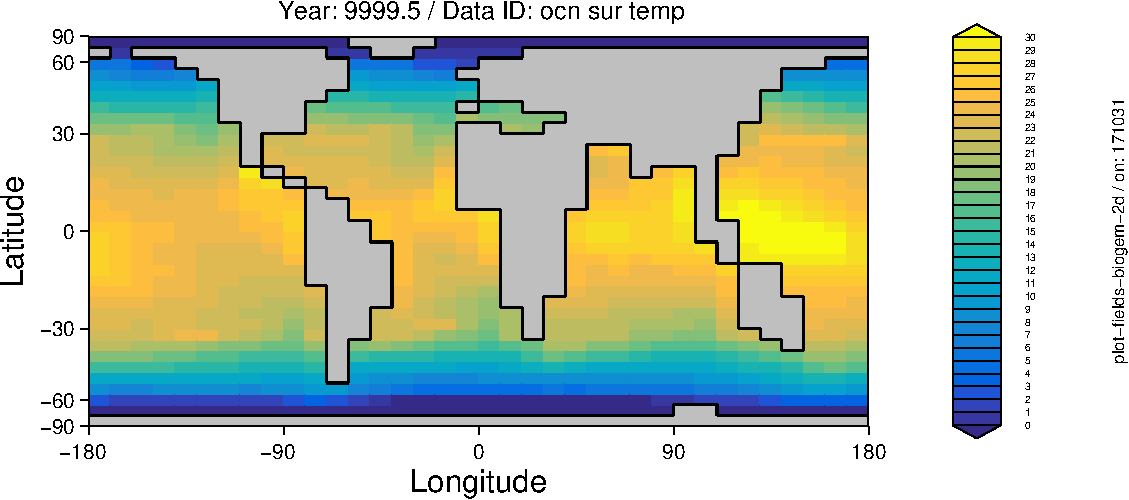
\includegraphics[scale=0.5]{example1a_171031.pdf}
\end{center}
\vspace{-4mm}
\caption{Example basic (default) surface temperature plot.}
\label{fig:example1a}
\end{figure}

For example:

\footnotesize
\vspace{-0pt}\begin{verbatim}
>> plot_fields_biogem_2d ...
('EXP1','','ocn_sur_temp','',9999.5,-1,16,'',1.0,0.0,30.0,30,'','','example1a');
\end{verbatim}\vspace{-0pt}
\normalsize
plots from the experiment \texttt{EXP1}, the variable \texttt{ocn\_sur\_temp} for time-slice \texttt{9999.5} (the mid-point time of the final year of a 10,000 year experiment). The color scale is from \texttt{0.0} to \texttt{30.0}, with no re-scaling (\texttt{1.0}), and \texttt{30} color intervals in the scale. The default \footnotesize\textsf{SETTINGS }\normalsize parameter file is used, and the default filename string replaced with \texttt{example1a}. The only other thing to note, is for parameter \texttt{PIK}, a value of \texttt{16} is set -- corresponding to the ocean surface. See Figure \ref{fig:example1a}.

Note that in this example, the   variable \texttt{ocn\_sur\_temp} is assumed. However, the model results variable \texttt{ocn\_sur\_temp} is not always saved in \textbf{BIOGEM} 2D netCDF output. If the requested variable, such as \texttt{ocn\_sur\_temp} does not exist, or is mis-spelt, \textbf{MATLAB} will pause and provide a warning. It will then list all the variables in the netCDF file that it can find and wait for a new variable name to be inputted. For instance, a variable that is always saved in \textbf{BIOGEM} 2D netCDF output is \texttt{atm\_temp} (surface air temperature) and could be substituted in the plot. Also note that time (the time-slice year to be plotted) is similarly handled -- if the specific time-slice value does not exist, a list of all possible time-slice years are provided and a substitute value requested as \textbf{MATLAB} pauses and wait for your input.

\begin{figure}[ht]
\begin{center}
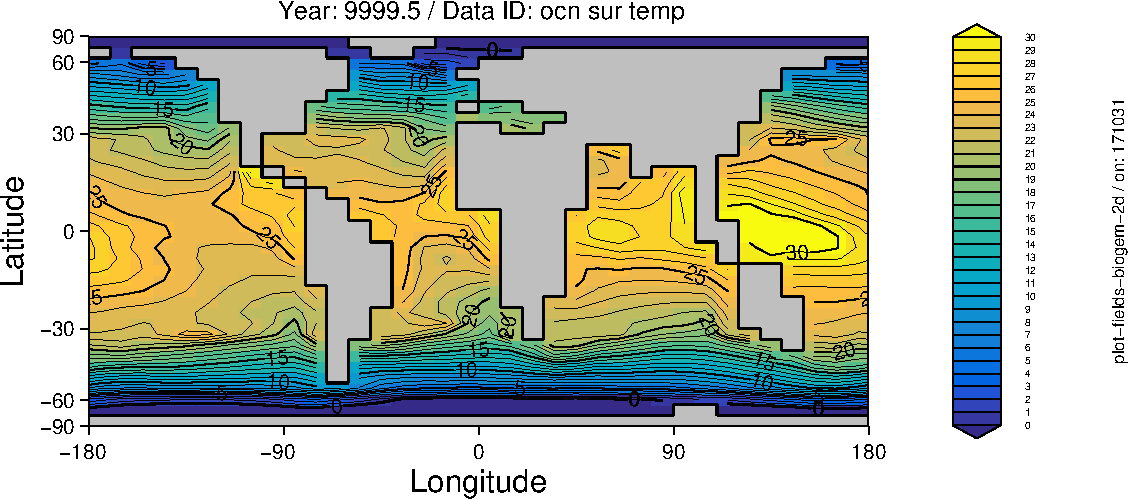
\includegraphics[scale=0.5]{example1b_171031.pdf}
\end{center}
\vspace{-4mm}
\caption{Example surface temperature plot, with contours.}
\label{fig:example1b}
\end{figure}

\vspace{4pt}
To add contours, in the default \footnotesize\textsf{SETTINGS }\normalsize parameter file (or a copied and re-named version thereof), adjust the following line:
\small
\vspace{-2pt}\begin{verbatim}
contour_plot = 'y';     % [ 'y']  OVERLAY CONTOUR PLOT?
\end{verbatim}\vspace{-2pt}
\normalsize
The results of this are shown in Figure \ref{fig:example1b}.

\pagebreak

Refinements to the contouring can be done by changing the lines:
\small
\vspace{-2pt}\begin{verbatim}
contour_mod = 1;        % [   1]  NUMBER OF COLOR INTERVALS PER CONTOR
contour_mod_label = 5;  % [   5]  NUMBER OF LABELED CONTOURS PER CONTOUR
contour_label = 'y';    % [ 'y']  LABEL CONTOURS?
contour_dashneg = 'n';  % [ 'n']  PLOT NEGATIVE CONTOURS DASHED?
\end{verbatim}\vspace{-2pt}
\normalsize
(these are the more commonly used refinements).

Here: \texttt{contour\_mod} determines how many color intervals per contour interval, which in the previous SST plot example, was \texttt{30}. So a value of \texttt{1} will give you 30 contours -- one every 1 degree C. And a value of \texttt{5} will give you 6 contours -- one each 5 degrees C.

\texttt{contour\_mod\_label} then determines whether you want the contours labelled or not. The answer (parameter value) to be the character \texttt{y} or \texttt{n}, as a string (i.e. in inverted commas). If you elect to have contour labels, \texttt{contour\_mod\_label} determines how frequently to label the contours. A value of \texttt{1} labels every single contour. A value of \texttt{2} labels every other contour. So for instance, if you set \texttt{contour\_mod=5} and \texttt{contour\_mod\_label=2} in the previous SST example, you get a contour every \texttt{5} degrees C, and a temperature label every \texttt{10} degrees C.

\vspace{4pt}
Alternatively, using 3d plotting, you could plot the ocean surface temperature field as follows:

\footnotesize
\vspace{-0pt}\begin{verbatim}
>> plot_fields_biogem_3d_k ...
('EXP1','','ocn_temp','',9999.5,-1,16,'',1.0,0.0,30.0,30,'','','example1c');
\end{verbatim}\vspace{-0pt}
\normalsize
The main things that change here are firstly the variable name -- now \texttt{ocn\_temp}, and secondly because this is a 3D ocean field, we need to specify what ocean model level we want to plot -- this is where the integer \texttt{16} comes in and corresponds to the input  \texttt{PIK}, as discussed earlier. The resulting plot will be identical to Figure \ref{fig:example1a}.

\vspace{4pt}
\item \textbf{Global zonal average temperature profile}

To keep with ocean temperature, we can use the \texttt{plot\_fields\_biogem\_3d\_i} function to plot the global zonal mean (lat-depth) profile (rather than horizontal, surface slice):

\footnotesize
\vspace{-0pt}\begin{verbatim}
>> plot_fields_biogem_3d_i ...
('EXP1','','ocn_temp','',9999.5,-1,0,'',1.0,0.0,30.0,30,'','','example2a');
\end{verbatim}\vspace{-0pt}
\normalsize
The only significant change as compared to before, is setting a \texttt{0} for input parameter \texttt{PIK} (again -- see earlier). The results is shown in Figure \ref{fig:example2a}.

\begin{figure}[ht]
\begin{center}
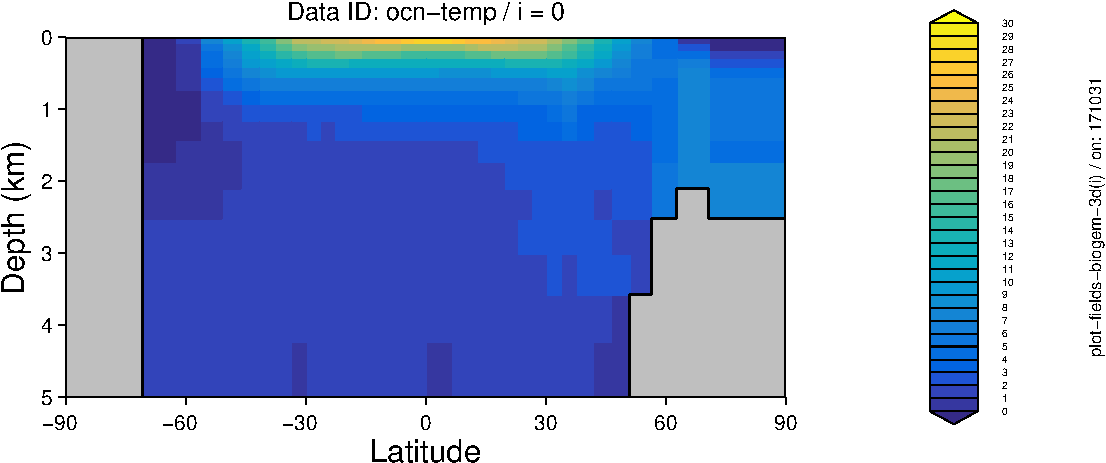
\includegraphics[scale=0.5]{example2a_171031.pdf}
\end{center}
\vspace{-4mm}
\caption{Zonal mean global ocean temperature profile.}
\label{fig:example2a}
\end{figure}

\vspace{4pt}
\item \textbf{Pacific dissolved oxygen profile}

As per choosing ocean levels (\texttt{k}-values) in the lon-lat plotting, you can also specify a specific longitude for creating a lat-depth section rather than calculating and plotting a global zonal mean. e.g. Figure \ref{fig:example3a} was created by\footnote{Also turning on the contour plotting.}:

\footnotesize
\vspace{-0pt}\begin{verbatim}
>> plot_fields_biogem_3d_i ...
('EXP1','','ocn_O2','',9999.5,-1,10,'',1.0E-6,0.0,300.0,30,'','','example3a');
\end{verbatim}\vspace{-0pt}
\normalsize
The chosen section is somewhere in the Pacific, along a line of longitude (whatever corresponds to \texttt{i=10} on this \textbf{muffin} model grid ... I guess about 165W ...). Here, the variable to be plotted has also been changed -- \texttt{ocn\_O2}\footnote{You'll need a biogeochemsitry enabled \textit{base-config}}. Because the units of dissolved oxygen are much smaller than for temperature (in degrees C),  the plotted scale has also been changed -- from 0 to 300 \(\mu mol kg^{-1}\) rather than the netCDF variable units of \(mol kg^{-1}\). To achieve this re-scaling, a units scaling value of \texttt{1.0E-6} is specified for parameter \texttt{PCSCALE}.\footnote{Note that the scaling specified is as the new units relative to the old units -- here, \(\mu mol kg^{-1}\) relative to \(mol kg^{-1}\) and hence \(10^{-6}\). ALSO NOTE that \textbf{Panoply} does it the other way around ... :(}

\begin{figure}[ht]
\begin{center}
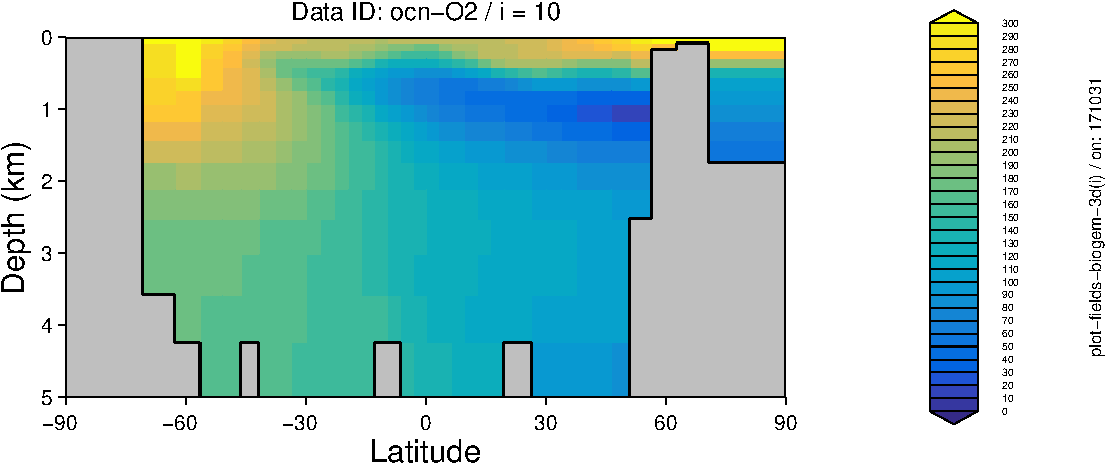
\includegraphics[scale=0.5]{example3a_171031.pdf}
\end{center}
\vspace{-4mm}
\caption{Ocean oxygen profile on a Pacific transect.}
\label{fig:example3a}
\end{figure}

\vspace{4pt}
\item \textbf{Atlantic zonal mean dissolved oxygen profile}

So far, with the exception of plotting a gridded color field \uline{and} a contoured field at the same time, all these examples can also be done in \textbf{Panoply}. One difference, is the ability in the \textbf{muffinplot} suite of \textbf{MATLAB} functions to apply masks -- isolating geographical regions or even single points. In the \footnotesize\textsf{MASKS }\normalsize directory, are a series of example ASCII mask files, mostly for the 2 (8- and 16-level ocean) modern published configurations of \textbf{muffin}. For instance, \footnotesize\textsf{mask\_worjh2\_AtlanticALL.dat }\normalsize has all the grid points in the entire Atlantic basin assigned a value of \texttt{1}, with \texttt{0} everywhere else. If we apply this first to the surface ocean dissolved oxygen field:

\footnotesize
\vspace{-0pt}\begin{verbatim}
>> plot_fields_biogem_3d_k ...
('EXP1','','ocn_O2','',9999.5,-1,16,'mask_worjh2_AtlanticALL.dat',1.0E-6,0.0,300.0,30,
... '','','example4a');
\end{verbatim}\vspace{-0pt}
\normalsize
we obtain Figure \ref{fig:example4a}.

\begin{figure}[ht]
\begin{center}
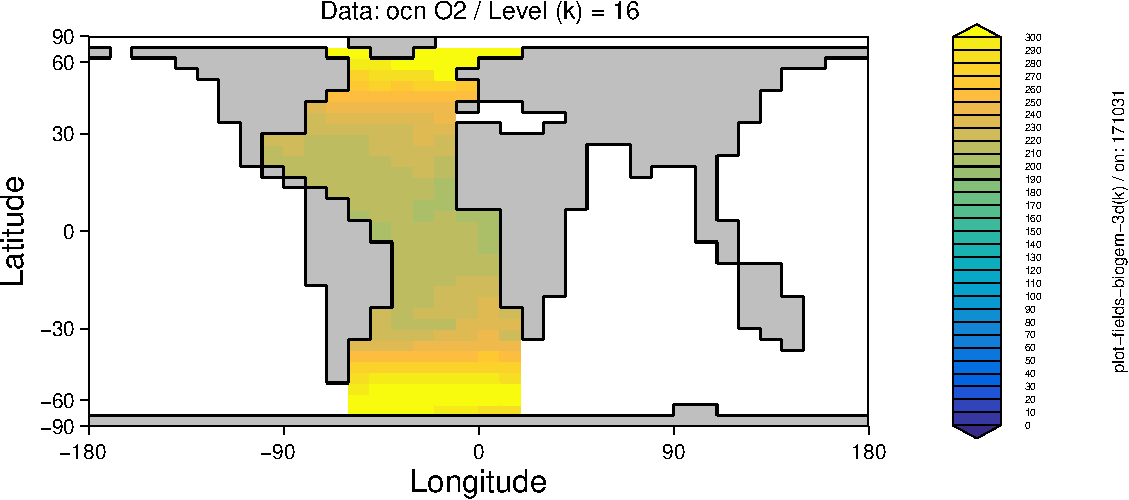
\includegraphics[scale=0.5]{example4a_171031.pdf}
\end{center}
\vspace{-4mm}
\caption{Distribution of surface ocean dissolved  oxygen in the Atlantic.}
\label{fig:example4a}
\end{figure}

Here, it is clear how the masked has been applied and all the ocean falling outside of the mask is plotted as white (no data).

We can also apply a mask field to the zonal average plot:

\footnotesize
\vspace{-0pt}\begin{verbatim}
>> plot_fields_biogem_3d_i ...
('EXP1','','ocn_O2','',9999.5,-1,0,'mask_worjh2_AtlanticALL.dat',1.0E-6,0.0,300.0,30,
... '','','example4b');
\end{verbatim}\vspace{-0pt}
\normalsize
(Figure \ref{fig:example4b})

\begin{figure}[ht]
\begin{center}
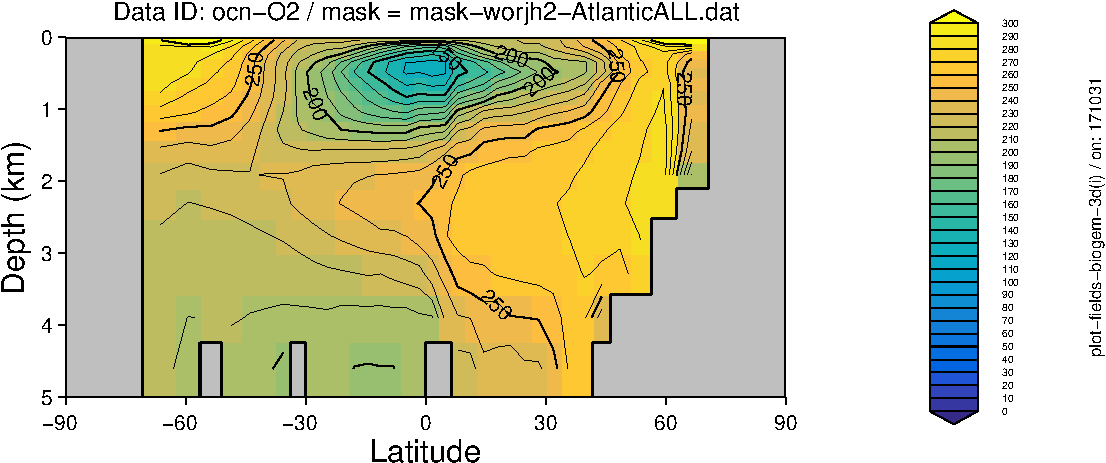
\includegraphics[scale=0.5]{example4b_171031.pdf}
\end{center}
\vspace{-4mm}
\caption{Mean zonal ocean oxygen profile in the Atlantic.}
\label{fig:example4b}
\end{figure}

\end{enumerate}

%------------------------------------------------

\subsection{Example analysis}

An set of \textbf{MATLAB} \footnotesize\textsf{m-file }\normalsize functions are provided that define a series of different generic and basic experiment analysis and plottings, with \footnotesize\textsf{make\_analysis\_ALL.m }\normalsize provided as a template for carrying them all out in one go. Obviously, the individual aggregate plotting functions can be edited, added to, or with unwanted or irrelevant plots, commented out or deleted -- treat these all simply as templates for developing your own analysis strategy (as well as viewing the associated configuration files as illustrations of the function/use of some of the different further plotting options\footnote{Also covered in a subsequent sub-sub-section.}).

The aggregate plotting functions are as follows:

\begin{enumerate}[noitemsep]

\vspace{1pt}
\item \footnotesize\textbf{\textsf{fun\_make\_analysis\_phys.m}}\normalsize \\This encompasses a basic set of analyses of ocean circulation and climatology.
\\The script is written as a \textit{function}, and requires just two parameters to be passed as input:
\begin{enumerate}[noitemsep]
\setlength{\itemindent}{.2in}
\item The experiment name.
\item The (mid-point of the) year of the time-slice to plot.
\end{enumerate}
In the example of an experiment called \texttt{'EXP1'}, and plotting the last annual time-slice (\texttt{9999.5}) from a 10,000 year model run, the function is hence called:
\vspace{-2pt}\begin{verbatim}
fun_make_analysis_phys('EXP1',9999.5);
\end{verbatim}\vspace{-2pt}

\vspace{1pt}
\item \footnotesize\textbf{\textsf{fun\_make\_analysis\_geo.m}}\normalsize \\This encompasses a basic set of analyses of ocean (abiotic) geochemistry and ocean acidification related variables and metrics.

\vspace{1pt}
\item \footnotesize\textbf{\textsf{fun\_make\_analysis\_bio.m}}\normalsize \\This encompasses a basic set of analyses of marine biological fluxes and biologically related properties.

\vspace{1pt}
\item \footnotesize\textbf{\textsf{fun\_make\_analysis\_ALL.m}}\normalsize
\\Aggregates all the above functions (i.e., calls all 3).
\end{enumerate}

\vspace{2pt}
To run these example analysis -- either copy all the files contained in the \footnotesize\textsf{EXAMPLES }\normalsize subdirectory, to your working directory (e.g. \footnotesize\textsf{RESULTS }\normalsize as per the previous example). Then type e.g..\footnote{Note that if you did not run with ocean biogeochemsitry (but rather climate-only), not all the plotting functions will run and you will have to restrict this default analysis to: \texttt{fun\_make\_analysis\_phys('EXP1',9999.5);}}

\vspace{-2pt}\begin{verbatim}
fun_make_analysis_ALL('EXP1',9999.5);
\end{verbatim}\vspace{-2pt}

\noindent OR, add the path to the \footnotesize\textsf{EXAMPLES }\normalsize subdirectory, e.g.
\vspace{-2pt}\begin{verbatim}
addpath('Y:\_git\muffinplot\EXAMPLES');
\end{verbatim}\vspace{-2pt}
but obviously depending on quite where you installed \textbf{muffinplot}.

%------------------------------------------------

\subsection{Further refinements}

A number of additional options for exerting finer control over the plotting are provided as a block of parameters and (default) values in the m-file itself, in a section immediately after the commented help and change-log at the start of the m-file. Not all the options are relevant to all the plotting functions\footnote{See 'help' on a specific plotting function for details of the relevant options in the parameter block.}, but the full list (and then defaults in brackets \texttt{[]}) is as follows:

\vspace{2pt}
{\small \begin{enumerate}
\item \texttt{lon\_min = -180;         [-180]  STARTING LONGITUDE FOR X-AXIS}
\\ Sets the longitude of the left-hand edge of the plot.
\item \texttt{delta\_lon = 90;         [  90]  INCREMENT OF LONGITUDE ON X-AXIS}
\\ Sets the longitude tick increment.
\item \texttt{contour\_plot = 'n';     [ 'n']  OVERLAY CONTOL PLOT?}
\\ Overlay line contours on the color block plot?
\item \texttt{contour\_mod = 2;        [   2]  NUMBER OF COLOR INTERVALS PER CONTOR}
\\ Number of color graduations per line contour.
\item \texttt{contour\_mod\_label = 4;  [   4]  NUMBER OF LABELED CONTOURS PER CONTOUR}
\\ Number of color graduations per labeled line contour.
\item \texttt{contour\_label = 'y';    [ 'y']  LABEL CONTOURS?}
\\ Label the line contours (frequency of labeled contours set by \texttt{contour\_label}.
\item \texttt{contour\_noneg = 'n';    [ 'n']  RESTRICT DATA PLOTTED TO > 0.0?}
\\ Restrict the plotted values to non-negative? (Can be useful if slightly negative values exist as can occur during tracer transport associated with large concentration gradients.)
\item \texttt{plot\_log10 = 'n';       [ 'n']  PLOT LOG10 OF THE DATA}
\\ Plot data values as log10(value)?
\item \texttt{contour\_zero = 'y';     [ 'y']  PLOT ZERO CONTOUR}
\\ Plot the zero contour?
\item \texttt{colorbar\_old = 'n';     [ 'n']  PLOT 'OLD' COLORBAR}
\\ Plot old style colorbar.
\item \texttt{data\_offset = 0.0;      [ 0.0]  data offset (273.15 for K -> C)}
\\ Introduce a data offset? This is useful for example for converting K to degrees C (removing the K value of 0 degrees C).
\item \texttt{data\_ij = 'n';          [ 'n']  DATA as (i,j)?}
\\ Overlay data in the form of (i,j) locations rather than longitude,latitude?
\item \texttt{data\_ijk = 'n';          [ 'n']  DATA as (i,j,k)?}
\\ Overlay data in the form of (i,j,k) locations rather than longitude, latitude, depth?
\item \texttt{data\_ij\_mean = 'n';     [ 'n']  average DATA by cell?}
\\ Average overlay data per \textit{c}GENIE grid cell rather than plotting raw locations.
\item \texttt{data\_ijk\_mean = 'n';     [ 'n']  average DATA by cell?}
\\ Average overlay data per \textit{c}GENIE grid cell rather than plotting raw locations.
\item \texttt{data\_size = 25.0;       [25.0]  SIZE OF OVERLAY DATA POINTS}
\\ Size of the overlay data points.
\item \texttt{data\_anomoly = 'n';     [ 'n']  PLOT AS MODEL-DATA ANOMOLY ONLY?}
\\ Plot data locations with the model-data anomaly rather than data value?
\item \texttt{data\_only = 'n';        [ 'n']  PLOT ONLY DATA (no model values)?}
\\ Plot only the overlay data locations (and not any model data)?
\item \texttt{data\_site = 'n';        [ 'n']  PLOT DATA AS SITES (no data values)?}
\\ Plot labeled site locations (no data value fill).
\item \texttt{plot\_land = 'n';        [ 'n']  PLOT DATA OVER LAND?}
\\ Plot data locations lying over land on the \textit{c}GENIE grid (rather than screen out)?
\item \texttt{data\_uv = 'n';          [ 'n']  overlay (u,v) velocity data?}
\\ Overlay ocean current fields.
\item \texttt{data\_uv\_scale = 1.0;    [ 1.0]  scaling factor for vector length}
\\ Scaling factor for velocity vectors.
\item \texttt{plot\_opsi = '';         [  '']  PLOT OVERTURNING STREAMFUNCTION (basin)?}
\\ Plot overturning streamfunction overlay?
\item \texttt{plot\_opsi\_min = -15;    [ -15]; plot\_opsi\_max = +15;    [ +15];
plot\_opsi\_dminor = 1;   [   1]; plot\_opsi\_dmajor = 5;   [   5] }
\\ Controls on min, max and (major and minor) contor intervals.
\item \texttt{dscrsz = 0.60;          [0.60]  FRACTIONAL FIGURE WINDOW SIZE}
\\ Adjustment factor of the fractional size (compared to the screen) of the figure window.
\end{enumerate}}
\vspace{2pt}

\subsubsection{Further refinements: Examples}

Examples:
\begin{enumerate}
\item To plot the positions (and labels) of data locations:
\\ {\small \texttt{plot\_fields\_biogem\_3d\_k('cgenie\_output','120926.SPIN','',49999.5,-1,'ocn\_temp','','',\\16,1.0,10.0,40.0,30,'','sites.dat')}}
\\ where the experiment name is \texttt{120926.SPIN}, the mapped variable is \texttt{ocn\_temp} (although no model field need be plotted -- set by an option in the plotting function itself, and the file of data locations is \texttt{sites.dat}.
\end{enumerate}

\begin{figure}[ht]
\begin{center}
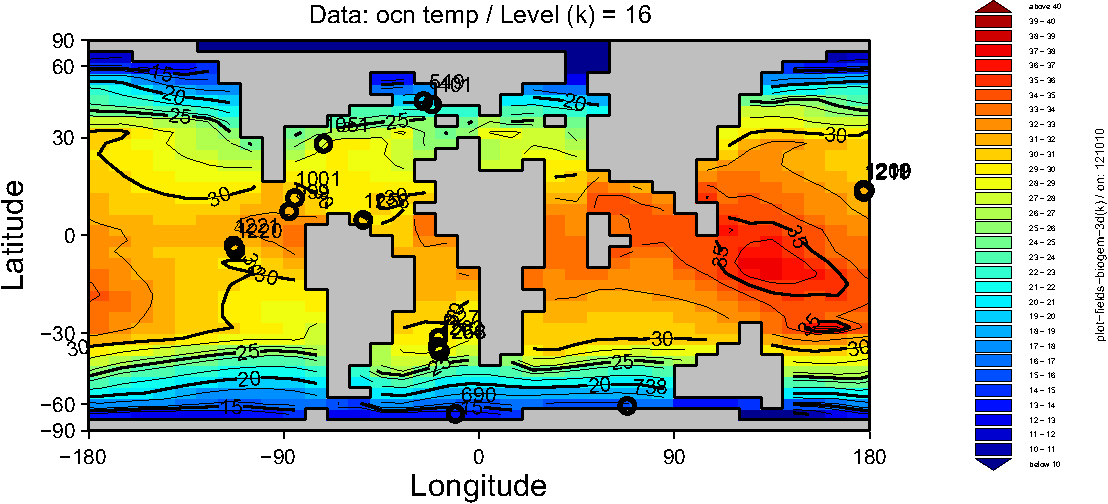
\includegraphics[scale=0.75]{cgenie_datalocations.pdf}
\end{center}
\caption{Paleocene-Eocene deep-sea sediment drill locations together with a contour-overlain map of surface temperature.}
\label{fig:cgenie_datalocations}
\end{figure}

%------------------------------------------------

\subsection{Time-series plotting}

%------------------------------------------------

\subsection{Sediment model output analysis}

%----------------------------------------------------------------------------------------
%       CHAPTER X
%----------------------------------------------------------------------------------------

\cleardoublepage

\chapterimage{big-data.jpg} % Chapter heading image

\chapter{muffindata}\label{ch:muffindata}

\hfill \break
\vspace{24mm}

%------------------------------------------------

\newpage

%------------------------------------------------

\section{Data re-gridding}

A number of \textbf{MATLAB} functions are available in \textbf{muffindata} for transforming data:

\vspace{1mm}
\begin{itemize}[noitemsep]
\vspace{1mm}
\item \textbf{make\_regrid\_data2ASCII\_GENIE.m}
\\Re-grids plain text (ASCII) point location data to a 2D \textbf{muffin} grid and saves as a 2D ASCII format file. 
\vspace{1mm}
\item \textbf{make\_regrid\_ASCII2netcdf\_GENIE.m}
\\Converts 2D \textbf{muffin} grid ASCII format data to \textbf{netCDF} format. 
\vspace{1mm}
\item \textbf{make\_regrid\_data2netcdf\_GENIE.m}
\\Re-grids plain text (ASCII) point location data to a 3D \textbf{muffin} grid and saves as \textbf{netCDF} format.
\vspace{1mm}
\item \textbf{make\_regrid\_data2netcdf\_WOA.m}
\\Re-grids plain text (ASCII) point location data to the standard 3D World Ocean Atlas grid and saves as \textbf{netCDF} format.
\vspace{1mm}
\item \textbf{make\_regrid\_WOA2GENIE.m}
\\Converts a 3D World Ocean Atlas grid netCDF variable to the \textbf{muffin} grid and saves as \textbf{netCDF} format (as well as ASCII).
\end{itemize}

%------------------------------------------------

\newpage

%------------------------------------------------

\section{Miscellaneous data processing}

%------------------------------------------------

\newpage

%------------------------------------------------

\section{Model ensembles}

The \textbf{muffindata} \textbf{MATLAB} file: \textsf{\footnotesize fun\_make\_ensemble\_2d.m} provides a simple/convenient way of generating ensembles of model experiments. By default, the function is designed for generating 2D ensembles of a first varying parameter vs. a second varying parameter. However, by specifying only a single value of the 2nd (or first) parameter, you'll obtain a 1D ensemble of just a single  parameter varying.

Information about how to configure and generate an ensemble is provided as \textbf{MATLAB} help on this function:
\vspace{-2mm}
\begin{verbatim}
>> help fun_make_ensemble_2d
\end{verbatim}
\vspace{-2mm}

The function \textsf{\footnotesize fun\_make\_ensemble\_2d.m} requires 2 parameters (\textit{strings}) to be passed in the argument list, i.e.:
\vspace{-1mm}\begin{verbatim}
>> fun_make_ensemble_2d.m(PAR1,PAR2)
\end{verbatim}\vspace{-1mm}
These are, in order:
\begin{enumerate}
\vspace{1mm}
\item \texttt{STR\_TEMPLATE} -- \textit{string} \(\rightarrow\) is the name of the template \textit{user-config} file (within the \textbf{muffindata} directory) used to generate the ensemble. 
\\Note that the \textit{user-config} may already contain a value for the varying parameter(s) -- the automatically-generated parameter values will be appended at the very end of the file, hence over-writing any previous values.
\vspace{1mm}
\item \texttt{STR\_PARAMS} -- \textit{string} \(\rightarrow\)  is the name of the parameter configuration file (omitting the '\textsf{\footnotesize .dat}' extension). The format of this file is plain text and takes a '\textsf{\footnotesize .dat}' extension. Example contents for this file are provided in the \textbf{MATLAB} help for this function.
\end{enumerate}
\vspace{2mm}

\noindent An example example usage  would be:
\vspace{-1mm}\begin{verbatim}
>> fun_make_ensemble_2d.m('user_config_template','ensemble_params')
\end{verbatim}\vspace{-1mm}
which creates an ensemble based on the \textit{user-config} file: \textsf{\footnotesize user\_config\_template} (example file name) and with varying parameter values specified in the file: \textsf{\footnotesize ensemble\_params.dat} (example file name).

The \textit{user-config} (and hence experiment names) that are automatically generated end in \textsf{\footnotesize .xy}, where \textsf{\footnotesize x} represents the \(x+1th\) parameter value on the first axis, and \textsf{\footnotesize y} represents the \(y+1th\) parameter value on the second axis (the \textsf{\footnotesize .xy} notation starts counting at \textsf{\footnotesize .00}). For instance, \textsf{\footnotesize .00} would be an experiment taking the first parameter values specified in \textsf{\footnotesize ensemble\_params.dat} for both axes. \textsf{\footnotesize .10} would have the 2nd lister parameter value on the 1st axis, and the 1st lister on the 2nd axis. \textsf{\footnotesize .27} would have the 3rd parameter value on the 1st axis, and 8th listed parameter value on the 2nd axis. etc etc etc

Also in \textbf{muffindata} you can find a BASH shell script for submitting the entire ensemble\footnote{Having first transferred all the \textit{user-config} files to the cluster to an appropriate \textsf{\footnotesize genie-userconfigs} folder} at the command line (within \textsf{\footnotesize genie-main}) -- \textsf{\footnotesize sub\_ens.muffin.sh}. NOTE: you have to specify the experiment parameters of your ensemble (e.g. \textit{base-config} and \textit{user-config} filenames, run duration, etc.) in the BASH file and you should be sure to have compiled the model (by running a brief experiment) with the required \textit{base-config} prior to using \textsf{\footnotesize sub\_ens.muffin.sh}.

The lines requiring editing in \textsf{\footnotesize sub\_ens.muffin.sh} are clearly marked and these instructions are not repeated here.

\newpage 

Note that you may need to re-assigned an 'executable' permission after editing and saving \textsf{\footnotesize sub\_ens.muffin.sh}. To do this, from \textsf{\footnotesize genie-main}:
\vspace{-1mm}\begin{verbatim}
>> chmod a+x sub_ens.muffin.sh
\end{verbatim}\vspace{-1mm}

\vspace{-2mm}
\noindent\rule{4cm}{0.5pt}
\vspace{2mm}

\noindent What do you then 'do' with a whole bunch of experiments with names ending in \textsf{\footnotesize .xy} ... ??? (Note that you can take any series of experiments, and rename such that they all have exactly the same filename with the exception of an \textsf{\footnotesize .xy} format extension. i.e. a series of 5 experiments with whatever varying filenames could become: \textsf{\footnotesize FILENAME.00}, \textsf{\footnotesize FILENAME.01}, \textsf{\footnotesize FILENAME.02}, \textsf{\footnotesize FILENAME.03}, \textsf{\footnotesize FILENAME.04}, which would create a 1-D (\(1\times 5\)) ensemble.)

You could of course, pick out individual ensemble member to plot and analyse, referring to the \textsf{\footnotesize ensemble\_params.dat} file where you specified the sequence of parameter values on both axes in order to identify the ensemble member you want. And/or ...

The \textbf{muffindata} \textbf{MATLAB} file: \textsf{\footnotesize fun\_process\_ensemble\_2d.m} provides a simple/convenient way of processing and visualizing ensembles of model experiments.

Information about how to configure and generate an ensemble is provided as \textbf{MATLAB} help on this function:
\vspace{-2mm}\begin{verbatim}
>> help fun_process_ensemble_2d
\end{verbatim}\vspace{-2mm}

The function \textsf{\footnotesize fun\_make\_ensemble\_2d.m} requires 3 parameters to be passed in the argument list, i.e.:
\vspace{-2mm}\begin{verbatim}
>> fun_process_ensemble_2d.m(PAR1,PAR2,PAR3)
\end{verbatim}\vspace{-2mm}
These are, in order:
\begin{enumerate}
\vspace{1mm}
\item \texttt{PAR1} -- \textit{string} \(\rightarrow\) is simply the ensemble name, but omitting the \textsf{\footnotesize .xy} numerical code of individual ensemble members). 
\vspace{1mm}
\item \texttt{PAR2} -- \textit{number} \(\rightarrow\) is the year of model data to extract. e.g. \texttt{9999.5} for the last year of a 10,000 year long run.
\vspace{1mm}
\item \texttt{PAR3} -- \textit{string} \(\rightarrow\) is a name to assign to the output files (e.g. giving you a potentially more meaningful set of filenames than simply re-using \texttt{PAR1}.
\end{enumerate}
\vspace{1mm}

Ensure that you either run \textsf{\footnotesize fun\_make\_ensemble\_2d.m} (or rather, the renamed copy of it) from the \textbf{muffindata} directory, or add a path in \textbf{MATLAB} to it. \uline{Also} add a path to \textbf{muffinplot} if you are going to process \textbf{netCDF} variables.

\vspace{2mm}

\noindent Within the code of \textsf{\footnotesize fun\_process\_ensemble\_2d.m} are instructions/directions as to how to extract specific variables. More advanced usage can statistically compare to data and calculate the goodness of fit of al the ensembles members, and even automatically identify and further process the 'best' (depending on the specific criteria for 'best').

\vspace{1mm}
Unlike creating ensembles, \textsf{\footnotesize fun\_process\_ensemble\_2d.m} needs to be directly edited (or rather: create a copy, rename the file \uline{and} the function name at the top of the file, and edit that). The basic set-up is as follows and requires 4 steps (which are clearly marked in the code):

\begin{enumerate}

\vspace{2mm}
\item Define the x-axis of the ensemble, under:
\vspace{-1mm}\small\begin{verbatim}
% --- STEP #1 ----------------------------------------------------------- %
% define ensemble x axis
\end{verbatim}\normalsize\vspace{-1mm}
Here, the number of strings defined in the array (structure) defines how many different parameter values are represented in the x-axis of the ensemble. This may be just one (for a 1-D parameter ensemble).
\\The strings are categorical and need not be numbers and are used to label the axis ticks (with one label corresponding to each different parameter in the 1st dimension of the ensemble).
\\This is also an x-axis label to set.

\vspace{2mm}
\item Define the y-axis of the ensemble, under:
\vspace{-1mm}\small\begin{verbatim}
% --- STEP #2 ----------------------------------------------------------- %
% define ensemble y axis
\end{verbatim}\normalsize\vspace{-1mm}
As per above.
\\Note that both x-axis and y-axis structures can contain a single string, in which case the ensemble is 0-D (\(1\times1\)) and consists of a single experiment.

\vspace{2mm}
\item Define any time-series variables to be extracted and plotted, under:
\vspace{-1mm}\small\begin{verbatim}
% --- STEP #3 ----------------------------------------------------------- %
% define time-series variables to extract and plot
\end{verbatim}\normalsize\vspace{-1mm}
Here, any time-series variables to be extracted are defined.
\\The format is:
\vspace{-1mm}\small\begin{verbatim}
  m = m+1;
  data(m).dataname = 'VARIABLE';
  data(m).datacol  = COLUMN;
  data(m).scale    = SCALE;
  data(m).dataunit = 'LABEL';
  data(m).minmax   = [MINIMUM MAXIMUM];
\end{verbatim}\normalsize\vspace{-1mm}
(The \texttt{m = m+1;} bit it important should should not be left out.)
\\These settings are:
\begin{itemize}[noitemsep]
\vspace{1mm}
\item \texttt{VARIABLE} -- Is the name of the time-series variable following the \textsf{\small biogem\_series\_} part of the filename and excluding the \textsf{\small .res} bit at the end. 
\\For example, atmospheric \(pCO_{2}\) would be specified by:
\vspace{-1mm}\small\begin{verbatim}
data(m).dataname = 'atm_pO2';
\end{verbatim}\normalsize\vspace{-1mm}
\vspace{1mm}
\item \texttt{COLUMN} -- Is the column number in the time-series file to be analysed. 
\\For atmospheric \(pCO_{2}\), a value of \(2\) would analyse the total inventory in units of \(mol\), while column \(3\) would give the concentration in units of \(atm\).
\vspace{1mm}
\item \texttt{SCALE} -- Scale the variable (by this factor)?
\\For example:
\vspace{-1mm}\small\begin{verbatim}
data(m).scale = 1.0E6;
\end{verbatim}\normalsize\vspace{-1mm}
would multiply the time-series value by \(10^{6}\) and in the example of atmospheric \(pCO_{2}\), produce the data in units of \(\mu atm\) (or \(ppm\)).
\\The scaling need not be a simple multiple of orders-of-magnitude, and e.g.
\vspace{-1mm}\small\begin{verbatim}
data(m).scale = 12.0E-15;
\end{verbatim}\normalsize\vspace{-1mm}
will convert \(molC\) into \(PgC\).
\vspace{1mm}
\item \texttt{LABEL} -- What you could like to appear alongside the scale bar ... traditionally the variable name (property displayed) and units.
\vspace{1mm}
\item \texttt{[MINIMUM MAXIMUM]} -- The scale for the data range.
\\For example, having scaled atmospheric \(pCO_{2}\) to units of \(ppm\), this might be (depending upon the experiment):
\vspace{-1mm}\small\begin{verbatim}
data(m).minmax = [200 1000];
\end{verbatim}\normalsize\vspace{-1mm}
\end{itemize}

\vspace{1mm}

A grid plot, along with a plain text file of the values, will be created for each defined variable. Missing experiments, variables, or time-points, will appear as a white square in the grid plot for that particular ensemble member.\footnote{So the ensembles need not be complete, or all the runs finished successfully.}
\\The format of the output filename is: \textsf{\footnotesize OUTPUTNAME.VARIABLENAME.COLUMN.ps}, where \textsf{\footnotesize OUTPUTNAME} is the string (3rd parameter) passed to the function (and whcih need not be the full expleriment name), \textsf{\footnotesize VARIABLENAME} is the name of the analysed variable as defined by \texttt{data(m).dataname} (see above), and \textsf{\footnotesize COLUMN} is the column of the time-series file analysed, as defined by \texttt{data(m).datacol} (also see above).
\\\uline{Be careful} -- the plain text file (\textsf{\footnotesize OUTPUTNAME.VARIABLENAME.COLUMN.dat}) of values is \uline{up-side-down} as compared to the orientation of the plot.

\vspace{2mm}
\item Define any \textit{time-slice} (\textbf{netCDF}) variables to be extracted and plotted.
\vspace{1mm}
\\This requires 2 parts:
\vspace{1mm}
\vspace{-1mm}\small\begin{verbatim}
% --- STEP #4a ---------------------------------------------------------- %
% define netCDF variables to extract and plot/analyse
\end{verbatim}\normalsize\vspace{-1mm}
Here, the format is identical to step \#3 (don't forget the \texttt{m = m+1;} bit!), with the exception of the variable name definition:
\vspace{-1mm}\small\begin{verbatim}
data(m).dataname = 'mean_Pacific_oxygen';
\end{verbatim}\normalsize\vspace{-1mm}
which is not used except in defining the output filename, and the column:
\vspace{-1mm}\small\begin{verbatim}
data(m).datacol = 0;
\end{verbatim}\normalsize\vspace{-1mm}
which is also irrelevant and can be assigned a value of e.g. zero.
\vspace{1mm}
\\The second part:
\vspace{-1mm}\small\begin{verbatim}
% --- STEP #4b ------------------------------------------ %
% extract and plot/analyse netCDF variables 
\end{verbatim}\normalsize\vspace{-1mm}
is a little more complicated, and very much depends on exactly what you 'want' from the 2- or 3-D netCDF that can be represented as a single value.
\vspace{1mm}
\\Common is to conduct some sort of statistical goodness-of-fit analysis of a model variable against observations, or perhaps the same variable in a different model experiment. One might also be interested in statistical or otherwise calculated summary properties of a 3-D field (or fields), such as mean, minimum or maximum values, or even over-turning circulation strength -- anything passed back as a single value from the \textbf{muffinplot} plotting functions can be visualized acorns the ensemble. Code can also be added as and when required, for further analysis of combinations of outputs.
\\Some examples are given in \texttt{help} for this function.
\\Missing experiments will be represented a white square in the output plot. However, the \textbf{muffinplot} functions are less forgiving when it comes to missing or incorrect variable names and time-slice times, and everything will stop until you provide a value input at the command-line.

\end{enumerate}




%----------------------------------------------------------------------------------------
%       CHAPTER X
%----------------------------------------------------------------------------------------

\cleardoublepage

%\chapterimage{Map_of_Earth_24.jpg} % Chapter heading image

\chapter{muffingen}\label{ch:muffingen}

\hfill \break
\vspace{24mm}

%------------------------------------------------

\newpage

\section{muffingen basics}

%------------------------------------------------

\subsection{overview of the muffingen software}

\textbf{muffingen} is a collection of \textbf{MATLAB} functions that can create all the configuration files (excluding optional climatic and biogeochemical \textit{forcing} fields) required by the cGENIE (\textbf{muffin}) Earth system model. \textbf{muffingen} is designed to take the output from a fully coupled GCM, particularly of past climates with different continental configurations, and re-grid the output needed by the \textbf{muffin} model, in the form of files of boundary conditions, all  saved  in their respective correct format. However, \textbf{muffingen} can also be used to draw conceptual alternative Earths (in terms of continental configuration). Again, saving the required \textbf{muffin} files in their appropriate formats.

As a \textbf{MATLAB} code, (only) very basic familiarity with using \textbf{MATLAB} at the command line is required. And a copy/license of the \textbf{MATLAB} software ... A sufficient grasp of \textbf{MATLAB} can be gained by going through the following sections/subsections of the \textsf{matlabananas} textbook, which can be found on \href{https://github.com/derpycode/matlabananas}{GitHub} (look for the PDF file compiled form the latex source -- \textsf{BANANAS.pdf}):

\vspace{2mm}
\begin{itemize}[noitemsep]
\item Section 1.1 -- The \textbf{MATLAB} interface and command line.
\item Section 1.6 -- Changing directories and file search paths.
\item Section 2.2 -- Using \textit{functions} ... of which \texttt{muffingen} is one.
\end{itemize}
\vspace{2mm}

%------------------------------------------------

\subsection{Installing muffingen}

The \textbf{muffingen} code is hosted on GitHub:

\vspace{2mm}
\href{https://github.com/derpycode/muffingen}{\texttt{https://github.com/derpycode/muffingen}}
\vspace{2mm}

There are 2 ways to get your mitts on the \textbf{muffingen} code:

\vspace{2mm}
\begin{enumerate}

\vspace{1mm}
\item By downloading an archive file, containing all the code etc. For this -- click on the \textcolor[rgb]{0,0.501961,0}{green} \textsf{\small{Clone or Download}} button, and select \textsf{\small{Download ZIP}}.
\\You then unpack/unzip the files and directory structure where you want it.
\\This [archive download] is a perfectly workable way to proceed\footnote{Note that this way, you will be unable to easily update the code with whatever new developments or bug fixes occur in the future, nor can propagate back any code changes that you might have made and might want to become part of the official \textbf{muffingen} code  (i.e. downloading the \textsf{zip} file becomes a one-off installation that loses its formal connection to the GitHub repository).} ...

\vspace{1mm}
\item Or you can \textit{clone} the repository to where you intend to run \textbf{muffingen}. Note that you will need a git client installed on your computer. There are GUI clients for git, or this can be done at the command line:

\vspace{-2mm}
\begin{verbatim}
$ git clone https://github.com/derpycode/muffingen.git
\end{verbatim}
\vspace{-2mm}

By doing this, you have created your own code repository (and an identical copy of the one hosted on GitHub). As part of the \texttt{git clone} command, you also automatically \textit{check out} (from your very own personal repository) a copy of the code.

\end{enumerate}
\vspace{2mm}

Note that you download or clone \textbf{muffingen} to the computer that you have \textbf{MATLAB} installed on and will use to run \textbf{muffingen} (i.e. not necessarily to the computer where \textbf{muffin} itself is run).

%------------------------------------------------

\newpage

\subsection{Running muffingen}

To use the \textbf{cGENIE.muffin} model configuration generator \textbf{muffingen} -- at the command line in \textbf{MATLAB}, simply type:

\vspace{-2mm}
\begin{verbatim}
>> muffingen('FILENAME')
\end{verbatim}
\vspace{-2mm}

\noindent where \texttt{FILENAME} is the name of an ASCII format configuration file (having a \texttt{.m} filename extension) that specifies the required settings (see subsequent section).

This file (\texttt{FILENAME.m}), must either be present in the directory where you installed \textbf{muffingen} (the directory where e.g. where the file \texttt{muffingen.m} is located) e.g. \textsf{C:\textbackslash muffingen}. In this case, your \textbf{MATLAB} working directory must also be  set to \textsf{C:\textbackslash muffingen}. Or, the \textbf{MATLAB} working directory and the file \texttt{FILENAME.m} can reside elsewhere (both directory locations must be the same however). In this case, you will then 'add' the location of \textbf{muffingen} to \textbf{MATLAB}'s search path by the \textbf{MATLAB} function \texttt{addpath}\footnote{Refer to the \textbf{MATLAB} '\textsf{bananas}' text for the syntax for using \texttt{addpath}.}.

The \textbf{muffingen} model configuration generator then starts, and depending on the specific settings in the configuration file, may require no user input, or may require user input, either because this option was requested, or because a re-gridding issue arose that requires manual intervention to resolve. A series of plots are created (and saved) as the configuration generation progresses together with the \textbf{muffin} model configuration files themselves. All the various steps plus details of how the contents of the configuration files are generated are reported at the command line, and saved in a n ASCII format \texttt{*.log} file for future reference.

Depending on the specific configuration file settings (see later), \textbf{muffingen} has 5 main modes of operation, which are summarized as follows (and described in more detail, along with specific examples, below):

\begin{enumerate}[noitemsep]
\setlength{\itemindent}{.2in}
\setcounter{enumi}{0}
\vspace{1mm}
\item \textbf{Configuration derivation based on re-gridding climate output from a GCM.}
\\ The most common usage of \textbf{muffingen}, and enabling a new (typically paleo) configuration to be derived from the output of a GCM experiment. Currently options for utilizing 4 different GCMs are provided: HadCM3(l) (\texttt{'hadcm3'} or \texttt{'hadcm3l'}), FOAM (\texttt{'foam'}), CESM (\texttt{'cesm'}), and ROCKEE-3D (\texttt{'rockee'}).
\vspace{1mm}
\item \textbf{Derivation based on re-gridding a high resolution input topography.}
\\ In this option -- \texttt{'mat'} -- a land-sea mask and ocean bathymetry are re-gridded from a high(er) resolution \textsf{\footnotesize .mat} (\textbf{MATLAB}) topography file. Zonal wind-stress and speed, and zonal planetary albedo, are prescribed.
\vspace{1mm}
\item \textbf{Derivation based on an existing model topography '\texttt{.k1}' file (or simplified \texttt{.k2}) format variant).}
\\ This option -- \texttt{'k1'} or \texttt{'k2'} -- allows a topography to be re-created, or adapted/altered, all directly from an existing model 'k1' file (and hence existing model configuration). Zonal wind-stress and speed, and zonal planetary albedo, are prescribed.
\vspace{1mm}
\item \textbf{Derivation based on a prescribed land-sea mask.}
\\ This option -- \texttt{'mask'} -- will create a new configuration from any specified land-sea mask, whether 'real' or completely hypothetical. Zonal wind-stress and speed, and zonal planetary albedo, are prescribed.
\vspace{1mm}
\item \textbf{From a blank (all ocean) initial template.}
\\ Finally, this option -- \texttt{''} -- enables a topography to be drawn by hand within \textbf{muffingen} and hence represents an interactive alternative to (4) (rather than editing a land-sea mask in a text editor). Zonal wind-stress and speed, and zonal planetary albedo, are prescribed.
\end{enumerate}

\vspace{2mm}
Also depending on the specific options, and particularly whether or not \texttt{opt\_user} is set to \texttt{true}, and editor window will open, firstly for changes to the land-sea mask to be made, then later for the ocean bathymetry to be edited. Finally, a window will open allowing 'island paths' to be edited. The latter may be needed if \textbf{muffingen} cannot unambiguously determine them unaided.

Once you have successfully run \textbf{muffingen}, copy/transfer the entire  configuration subdirectory (the directory with the same name as whatever you called your 'world')  and its contents, from the \textbf{muffingen} output directory (e.g. \textsf{\small muffingen/OUTPUT.EXAMPLES}) on your local computer, to: \textsf{\footnotesize cgenie.muffin/genie-paleo}.

%------------------------------------------------

\newpage

\section{Configuring muffingen -- overview}

%------------------------------------------------

When \textbf{muffingen} is run, a configuration file with a specified filename\footnote{i.e. the single parameter passed to \textbf{muffingen} when it is invoked at the command line.} is loaded. The configuration file is in a simple plain text (ASCII) format, but is given a \textsf{.m} extension, enabling the values of a number of controlling parameter values to be set directly in \textbf{MATLAB}.\footnote{Note that the parameter filename is passed as a string without the .m extension (which is implicitly assumed). An error message will be generated if the file does not exist or has the incorrect extension.} The configuration file parameters control facets of \textbf{muffingen} behavior such as the primary model of operation, input and output filenames, what types of configuration files you want to generate, as well as there being a number of parameters controlling the finer details of re-gridding and configuration file generation, including whether to enable user-input or not.

The configuration files can be edited with the \textbf{MATLAB} editor (indeed, as a \textsf{\small .m} file, they are inherently a \textbf{MATLAB} format file), or any plain text (ASCII) editor. They must have a \textsf{\small .m} filename extension.
The configuration file is divided up into a series of sections of different parameter options. The main (most commonly used) parameters are summarized as follows (and are more fully described later):

\begin{itemize}

\vspace{2mm}
\item []
\small\vspace{-2pt}\begin{verbatim}
% *** CONFIG NAME AND MAIN INPUT SETTINGS *******************************
\end{verbatim}\vspace{-2pt}\normalsize

\begin{itemize}[noitemsep]
\vspace{1mm}

\item [] \texttt{par\_wor\_name}
\\Defines the name of the model configuration. This must be a string, \uline{8 characters long}.
\\e.g. \texttt{par\_wor\_name='my\_world'}

\item [] \texttt{par\_gcm}
\\Defines the format of the input. The string is blank for an interactive user-defined world, i.e. \texttt{par\_gcm=''}


\item [] \texttt{par\_expid}
\\Defines the name of the GCM experiment if a GCM input is selected, or the '\textsf{\small .k1}' or '\textsf{\small .dat}' files if those respective input formats are selected by the above option.
\\By default, these files live in the \textsf{\small INPUT.EXAMPLES} sub-directory.

\end{itemize}

\vspace{2mm}
\item []
\small\vspace{-2pt}\begin{verbatim}
% *** FILE PATHS ********************************************************
\end{verbatim}\vspace{-2pt}\normalsize

\vspace{2mm}
\item []
\small\vspace{-2pt}\begin{verbatim}
% *** GCM netCDF FILENAMES **********************************************
\end{verbatim}\vspace{-2pt}\normalsize

\vspace{2mm}
\item []
\small\vspace{-2pt}\begin{verbatim}
% *** GRID RESOLUTION ***************************************************
\end{verbatim}\vspace{-2pt}\normalsize

\begin{itemize}[noitemsep]
\vspace{1mm}

\item \texttt{par\_max\_i}
\\Defines the number of grid points in the longitude ('i') direction.
\\This is typically 36 or 18, e.g. \texttt{par\_max\_i=36}

\item \texttt{par\_max\_i}
\\Defines the number of grid points in the latitude ('j') direction.
\\This is typically 36 or 18 and is typically the same number as for the i direction, e.g. \texttt{par\_max\_j=36}

\item \texttt{par\_max\_k}
\\Defines the number of  layers in the ocean circulation model.
\\This is almost always either 16 or 8, e.g. \texttt{par\_max\_k=16}

\item \texttt{opt\_equalarea} [default: \texttt{true}]
\\This specifies whether or not an equal area grid is used/assumed. (A value of \texttt{false} results in the latitude grid being defined in equal increments of latitude).

\end{itemize}

\pagebreak

\vspace{2mm}
\item []
\small\vspace{-2pt}\begin{verbatim}
% *** REGRIDDING SETTINGS ***********************************************
\end{verbatim}\vspace{-2pt}\normalsize

\begin{itemize}[noitemsep]
\vspace{1mm}
\item [] \texttt{par\_max\_D} [default: \texttt{5000.0}]
\\Sets the maximum ocean (scale) depth (in m).
\\ See subsequent sub-sub-section on 'Ocean depth (and maximum levels)' for further details and usage.
\vspace{1mm}
\item [] \texttt{par\_sed\_Dmin} [default: \texttt{1000.0}]
\\\texttt{par\_sed\_Dmax} [default: \texttt{5000.0}]
\\Together, set the minimum and maximum depths used in generating a random seafloor topography for \textbf{SEDGEM} (when \texttt{par\_sedsopt=2} is selected).
\\Note that while \(5000m\) corresponds to the default deepest depth of the ocean circulation model, about \(15\%\) of the modern seafloor lies below this (and mostly shallower than \(6000m\)). So selecting \texttt{6000.0} would arguably enable a better simulation of e.g. the CCD. 
\end{itemize}

\vspace{2mm}
\item []
\small\vspace{-2pt}\begin{verbatim}
% *** CONFIG NAME AND MAIN INPUT SETTINGS *******************************
\end{verbatim}\vspace{-2pt}\normalsize

\begin{itemize}[noitemsep]
\vspace{1mm}

\item [] \texttt{opt\_user} [default: \texttt{true}]
\\Determines whether \textbf{muffingen} pauses and allows user-modification of land-sea mask and ocean depth (and island paths).
\end{itemize}

\end{itemize}

%------------------------------------------------

\subsection{muffingen configuration examples}

A series of example configurations are provided in the main \textbf{muffingen} directory. These illustrate parameter settings and the primary ways of using \textbf{muffingen}. They also serve as useful template parameter setting files.  They are:

\vspace{1mm}
\begin{itemize}[noitemsep]

\vspace{1mm}
\item \textsf{\footnotesize EXAMPLE\_BLANK} -- Starts from a blank ('water-world') all-ocean land-sea mask template. User input (allowing continents and seafloor topography to be 'drawn') is automatically activated whether you want it or not!\footnote{Because it assumes that you are going to go on and draw something ...}\(^{,}\)\footnote{Edit the \textbf{muffingen} code to be able to turn off.}

\vspace{1mm}
\item \textsf{\footnotesize EXAMPLE\_BLANK\_deep} -- As above, except with a deeper ocean -- 18 levels with the first 16 spanning 5000.0 m.\footnote{Refer to subsequence explanation re. the details of these parameters.}

\vspace{1mm}
\item \textsf{\footnotesize EXAMPLE\_MASK\_drakeworld} -- The first of a series of 4 conceptual worlds (loosely following the literature). This starts from a land-sea mask (\footnotesize\textsf{wordrake.dat}\normalsize) which is stored in the \textbf{muffingen} subdirectory \footnotesize\textsf{INPUT.EXAMPLES}\normalsize. The land fraction is minimal (as it is trying to reproduce the sort of zero-area numerical barrier used in the literature). This configuration has a barrier to ocean circulation, from the N pole down, with a high southern latitude gateway (a Drake Passage like feature).

\vspace{1mm}
\item \textsf{\footnotesize EXAMPLE\_MASK\_eqpasworld} -- As above, except with an equatorial (only) gateway.

\vspace{1mm}
\item \textsf{\footnotesize EXAMPLE\_MASK\_ridgeworld} -- As above, except with no gateway.

\vspace{1mm}
\item \textsf{\footnotesize EXAMPLE\_MASK\_waterworld} -- As above, but with no barriers, i.e. a 'water world'.

\vspace{1mm}
\item \textsf{\footnotesize EXAMPLE\_GCMFOAM\_modern} -- Takes the continental configuration and climate simulation output from a fully coupled GCM experiment (files in directory \footnotesize\textsf{GCMFOAM }\normalsize in the \textbf{muffingen} subdirectory \footnotesize\textsf{INPUT.EXAMPLES }\normalsize) and derives full \textbf{muffin} model boundary conditions. User input (allowing continents and seafloor topography to be 'edited') is activated by default.

\vspace{1mm}
\item \textsf{\footnotesize EXAMPLE\_GCMHadCM3L\_modern} -- Similar to the above -- takes the continental configuration and climate simulation output from a fully coupled GCM experiment (files in directory \footnotesize\textsf{GCMHadCM3L }\normalsize in the \textbf{muffingen} subdirectory \footnotesize\textsf{INPUT.EXAMPLES }\normalsize) and derives full \textbf{muffin} model boundary conditions. User input (allowing continents and seafloor topography to be 'edited') is activated by default.

\vspace{1mm}
\item \textsf{\footnotesize EXAMPLE\_K1\_permian} -- Starts from a muffin model configuration 'k1' topography defining file: \textsf{\footnotesize p0251b.k1}, which is stored in the \textbf{muffingen} subdirectory \texttt{INPUT.EXAMPLES}. The k1 file defines a late Permian continental configuration (and bathymetry). User modification is enabled by default (so \textbf{MATLAB} pauses for modifications to be made), but this can be disabled (\texttt{opt\_user=false}).

\vspace{1mm}
\item \textsf{\footnotesize EXAMPLE\_K2\_supercontinent} -- Starts from a simplified version of the muffin model configuration 'k1' topography defining file -- here given  the extension 'k2'. This (\textsf{\footnotesize wppcont1.k2}) is stored in the \textbf{muffingen} subdirectory \texttt{INPUT.EXAMPLES}. The k2 file defines an idealized pole-to-pole super-continent. User modification is enabled by default (so \textbf{MATLAB} pauses for modifications to be made), but this can be disabled (\texttt{opt\_user=false}).

\vspace{1mm}
\item \textsf{\footnotesize EXAMPLE\_K1\_SEDGEMonly} -- Similar to \textsf{\footnotesize EXAMPLE\_K1\_permian} -- starts from a muffin model configuration 'k1' topography defining file: \textsf{\footnotesize p0251b.k1}, but only generates the SEDGEM sediment model files (and nothing else).

\vspace{1mm}
\item \textsf{\footnotesize EXAMPLE\_MAT\_present\_bathymetry} -- Takes as input a high resolution topography in a \textbf{MATLAB} \textsf{\footnotesize .mat} file format. In this specific example, the file (subdirectory \texttt{INPUT.EXAMPLES}) inputted is \textsf{\footnotesize present\_bathymetry} (\textsf{\footnotesize .mat}) which describes at \(1^{\circ}\) resolution, the modern plate configurations plus seafloor topography (as negative height).\footnote{The specific grid resolution is defined, and the file loaded and the grid orientation assumed, in the \texttt{LOAD GRID (AXES) DATA} and \texttt{LOAD TOPO \& MASK DATA} sections. Different resolutions and orientations (and file formats) can be dealt with here by editing the code.}
\\If you want anything other than a \(1^{\circ}\) resolution (or a different longitude origin) then you need to edit the code:
\small\begin{verbatim}
% NOTE: assume equal Dlon, Dlat grid (non equal area) and 1 degree
%       also that the input grid starts at -180E
% >>> EDIT ME >>>>>>>>>>>>>>>>>>>>>>>>>>>>>>>>>>>>>>>>>>>>>>>>>>>>>
gi_lonce = [-180.0:1.0:180.0];
gi_latce = [-90.0:1.0:90.0];
% <<<<<<<<<<<<<<<<<<<<<<<<<<<<<<<<<<<<<<<<<<<<<<<<<<<<<<<<<<<<<<<<<
\end{verbatim}\normalsize
Non-rectilinear grids are not supported. If you have 3 poles in your grid ... too bad.

\end{itemize}
\vspace{2mm}

%------------------------------------------------

\newpage

\section{Pre-generated worlds}

A series of conceptual ('fake') worlds have been generated and are provided for you convenience :o) These fall into 2 categories:

\begin{enumerate}[noitemsep]
\vspace{1mm}
\item Conceptual worlds
\\These include 'water world', 'ridge world', 'drake world', etc. and associated variants, e.g. as published in fully coupled GCMs\footnote{Example of aquaplanets and drake worlds in the MITgcm with simplified atmosphere:
\\Rose, B. E. J., Ferreira, D. \& Marshall, J. The role of oceans and sea ice in abrupt transitions between multiple climate states. J. Clim. 26, 2862–2879 (2013).
\\Ferreira, D., Marshall, J. \& Rose, B. Climate determinism revisited: Multiple equilibria in a complex climate model. J. Clim. 24, 992–1012 (2011).}. They are designed to test controls on large-scale ocean circulation and do conform to an Earth-appropriate ocean volume or total cratonic area.
\vspace{1mm}
\item Idealized-continent worlds
\\These involve idealized super-continental configurations but aim to retain modern ocean volume and total cratonic area characteristics.
\end{enumerate}
\vspace{1mm}

Both \textsf{\footnotesize genie-paleo} configuration file sets (sub-directories), and example \textit{base-configs} are provided as part of the muffin code base. The details of these two series of fake worlds are as follows. Remember that the \textsf{\footnotesize .m} file configurations that create each of the fake world configurations are saved in the respective \textsf{\footnotesize genie-paleo} sub-directory, and hence both the specific details of how the world was created are available, as well as the ability to exactly recreate the world.

%------------------------------------------------
%
\subsection{Conceptual worlds}

\small\begin{itemize}[noitemsep]
\vspace{1mm}
\item \textsf{\footnotesize }
\item \textsf{\footnotesize }
\item \textsf{\footnotesize }
\item \textsf{\footnotesize }
\item \textsf{\footnotesize }
\item \textsf{\footnotesize }
\end{itemize}\normalsize
\vspace{1mm}

%------------------------------------------------
%
\subsection{Idealized-continent worlds}

The idealized continents come both without (i.e. the configuration is either land, or deep ocean) or with, continental shelves, and in the latter case, come with varying number of 'steps' down to deeper water (and hence to the abyssal plain).

The fake world series 'k1' configuration names start with one of two, 4 character strings:
\begin{itemize}[noitemsep]
\vspace{1mm}
\item \textsf{\footnotesize fkh\_} == 'high' resolution (\(36\times36\times16\))
\item \textsf{\footnotesize fkl\_} == 'low' resolution (\(18\times18\times16\))
\end{itemize}
\vspace{1mm}
\noindent (No low vertical resolution, e.g. \(8\) level version is currently provided.)
\vspace{1mm}

The next 2 characters delineate the shape/position of the world:
\begin{itemize}[noitemsep]
\vspace{1mm}
\item \textsf{\footnotesize 1e} == a single Equatorial-centered super-continent
\item \textsf{\footnotesize np} == a singleNorth polar-centered super-continent
\item \textsf{\footnotesize pp} == a pole-to-pole super-continent
\end{itemize}
\vspace{2mm}

The 7th character is the 'series' represents:
\begin{itemize}[noitemsep]
\vspace{1mm}
\item \textsf{\footnotesize 0} == An earlier generation of worlds, with shelves stepping down in increments of only \(1\) ocean level.
\\Note that in generating the wind-stress in this series, the presence/absence of high latitude gateways is automatically identified (meaning that the zonal wind-stress profiles differ between \textsf{\footnotesize np} and \textsf{\footnotesize pp} in the magnitude of wind-stress in the Southern Hemisphere) -- \texttt{par\_tauopt=0}.
\vspace{1mm}
\item \textsf{\footnotesize 1} == A subsequent generation, with shelves stepping down in increments of 2 ocean levels.
\\Note: An intermediate wind-stress magnitude is applied to both hemispheres in all configurations (i.e. no distinction is made between hemisphere with or without high latitude gateways) -- \texttt{par\_tauopt=3} .
\vspace{1mm}
\item \textsf{\footnotesize 2} == A modification of \#1,  generated with a newer version of \textbf{muffingen}, and with an imposed limit of \(1000-5000 m\) for the range of \textbf{SEDGEM} open ocean depths (the previous version included   depths extending to the shallow sub-surface).
\\Note that \texttt{par\_tauopt=0} is used. 
\\Also note that in \textsf{\footnotesize pp}, shelves are only created on the Eastern margin of the basin so as to retain consistency in total shelf area with  \textsf{\footnotesize np}.
\end{itemize}
\vspace{2mm}

The 8th character (digit) specifies the number of shelves, which for the initial series is:

\vspace{1mm}
\small\begin{enumerate}[noitemsep]
\setlength{\itemindent}{.2in}
\setcounter{enumi}{-1}
\item (none)
\item level \(15\)
\item level \(15 + 14\)
\item level \(15 + 14 + 13\)
\item level \(15 + 14 + 13 + 12\)
\item level \(15 + 14 + 13 + 12 + 11\)
\end{enumerate}\normalsize
\vspace{1mm}
and for the newer series:
\small\begin{enumerate}[noitemsep]
\setlength{\itemindent}{.2in}
\setcounter{enumi}{-1}
\item (none)
\item level \(15\)
\item level \(15 + 13\)
\item level \(15 + 13 + 11\)
\item level \(15 + 13 + 11 + 9\)
\end{enumerate}\normalsize
\vspace{1mm}

All the oceans are ca. \(3500 m\) deep, i.e. truncated at ocean level \(3\), in order to produce approximately the present-day ocean volume.\footnote{To change this, simply search-and-replace the \texttt{3} in the \textsf{\footnotesize .k1} file with e.g. \texttt{1}.}

Example \textit{base-configs} are provide for some, but not all of the idealized worlds, and follow the same naming convention and have full filenames of the form: \textsf{\footnotesize muffin.CB.\(\ast\ast\ast\ast\ast\ast\ast\ast\).BASES.config}, where \(\ast\ast\ast\ast\ast\ast\ast\ast\) is the 8-character fake world 'k1' configuration name (see above). A basic set of tracers is provided (\textsf{\footnotesize BASES}).

Other than the rate at which the shelves step down\footnote{(and that the earlier generation was for a pole-to-pole super-continent only)}, the main difference between the different generations of worlds, is in the applied zonal wind field strength. In the earlier fake world series, the 'zonal wind-stress generation option' (\texttt{par\_tauopt}) was \texttt{0}. This attempts to automatically determine the presence of high latitude ocean gateways and if they exist, apply a stronger zonal wind field in that hemisphere (otherwise, a wind stress appropriate for a modern northern-hemisphere configuration with no zonal gateway is applied). To reduce the number of boundary conditions that change and co-vary between different fake worlds, in the second generation of idealized continent worlds, an intermediate strength zonal wind field is applied to all, regardless of the presence of absence of high latitude circumpolar ocean gateways. This is  'zonal wind-stress generation option' \texttt{3}. Note that for the same resolution, wind-fields can be substituted/replaced, and using the saved \textsf{\footnotesize .m} configuration file, worlds can be re-generated with different wind-stress options if desired. The depth range of the ocean floor in\ \textbf{SEDGEM} (which informs the pressure used in the \(CaCO_{3}\) stability calculation) is slightly restricted in \#3 (the upper limit increased to \(1000 m\)).

%------------------------------------------------
%
\subsection{Modern worlds}

To both help illustrate how the configuration files are organized and accessed for paleo worlds, and to help make modifying older (modern) configurations easier, the 2 basic modern configurations are provided in a genie-paleo format:
\begin{itemize}[noitemsep]
\vspace{1mm}
\item \textsf{\footnotesize p\_worbe2} == The 8-level \(36\times36\) ocean configuration of \textit{Ridgwell et al.} [2007] and including the geological carbon cycle (\textbf{SEDGEM}+\textbf{ROKGEM}) configuration files of \textit{Ridgwell and Hargreaves} [2007] (and \textit{Lord et al.} [2015]).
\vspace{1mm}
\item \textsf{\footnotesize p\_worjh2} ==  The 16-level \(36\times36\) ocean configuration of \textit{Cao et al.} [2009] and including the geological carbon cycle (\textbf{SEDGEM}+\textbf{ROKGEM}) configuration files of \textit{Archer et al.} [2009] (and \textit{Winkelmann et al.} [2015]).
\end{itemize}

\vspace{2mm}
\noindent Corresponding example \textit{base-} and \textit{user-config} files are provided:
\begin{itemize}[noitemsep]
\vspace{1mm}
\item \textsf{\footnotesize muffin.CBSR.p\_worbe2.BASES.config} plus: \textsf{\footnotesize muffin.CBSR.p\_worbe2.BASES.SPIN1} \\(in: \textsf{\footnotesize genie-userconfig/EXAMPLES}), which runs the first-stage spin-up described in \textit{Ridgwell and Hargreaves} [2007] (and also used in \textit{Lord et al.} [2015]).
\vspace{1mm}
\item \textsf{\footnotesize muffin.CBSR.p\_worjh2.BASES.config} plus: \textsf{\footnotesize muffin.CBSR.p\_worjh2.BASES.SPIN1} \\(in: \textsf{\footnotesize genie-userconfig/EXAMPLES}), which runs the first-stage spin-up used in \textit{Archer et al.} [2009] and \textit{Winkelmann et al.} [2015].
\end{itemize}

\vspace{2mm}
\noindent To make modified (e.g. wind fields) versions of either of the 2 modern 'paleo' format configurations:
\begin{enumerate}[noitemsep]
\vspace{1mm}
\item Copy and rename the  (8- or 16-level ocean configuration) \textsf{\footnotesize genie-paleo} sub-directory, giving it an \uline{8 (or 6) character string name}.
\vspace{1mm}
\item In this new sub-directory, edit the files (wind stress, wind velocity, wind speed, albedo, and/or topography) you want to modify. (These files do not need to be renamed.)
\vspace{1mm}
\item Copy and rename the corresponding \textit{base-config} file (disabling the parameter settings for \textbf{SEDGEM} and \textbf{ROCKGEM}, and/or enabling \textbf{ECOGEM}, as required).
\\Then, in the \textit{base-config} file, edit all instances of the \textsf{\footnotesize genie-paleo} subdirectory parameters  to match the new \textsf{\footnotesize genie-paleo} sub-directory you assigned in step (1). (Parameters, e.g.: \textsf{\footnotesize ea\_1='../../cgenie.muffin/genie-paleo/p\_worbe2'}.
\vspace{1mm}
\item Copy-rename the example \textit{user-config}, or modify your own existing one.
\\Note that when employing the geological carbon cycle, the resolution of the sediment (and weathering) grids and associated boundary condition files are now defined in the \textit{base-config} rather than the \textit{user-config} (as originally done).
\end{enumerate}

%------------------------------------------------
%
%
%------------------------------------------------

\newpage

\section{Configuring muffin experiments}

%------------------------------------------------

Having created a new \textbf{muffin} configuration using the \textbf{MATLAB} function \textsf{\footnotesize muffingen.m}, you are now going to need to create 2 files before you can run any experiments:

\begin{enumerate}[noitemsep]
\vspace{1mm}
\item A \textit{base-config}, which includes the parameter settings of your new world.
\\There will there be 4 steps involved in this:
\begin{enumerate}[noitemsep]
\item Choosing a template \textit{base-config} file, which specifies appropriate physics parameters.
\item Copy-pasting a list of parameter settings that has been automatically-generated by \textbf{muffingen} into the template\textit{ base-config} file.
\item Defining the number of dissolved and particulate tracers in the ocean (and gases in the atmosphere) that you want and entering this into the \textit{base-config}.
\item Ensure that the appropriate science modules are enabled in the \textit{base-config}.
\end{enumerate}
\vspace{1mm}
\item A \textit{user-config}, whether simply to test the configuration or to provide the basis of a series of experiments.
\end{enumerate}
\vspace{1mm}

Templates are provided and more detailed instructions follow. However, note that if you have similar \textit{base-config} and \textit{user-config} files already, then you can simply adapt these. Another option is to utilize \textit{base-config} and \textit{user-config} files associated with any of the published experiments listed in \textsf{\footnotesize genie-userconfigs/MS}, or any of the described \textsf{\footnotesize EXAMPLE.*} example configurations.

Note that steps 1c, 1d, and 2 are not independent of each other and need to be consistent -- e.g. if you define Fe co-limitation of biological productivity in step 2, you need to have selected the appropriate tracers in step 1c. And if you specify biological productivity calculated by \textbf{ECOGEM} in step 2, you need to have selected the \textbf{ECOGEM} module in step 1d.

Finally ...
\begin{enumerate}[noitemsep]
\vspace{1mm}
\setcounter{enumi}{2}
\item You will need to ensure that all file are in their correct location in the directory structure.
\end{enumerate}
\vspace{1mm}


%------------------------------------------------
%
\noindent\rule{4cm}{0.5pt}
\subsubsection{1a. Choosing a template \textit{base-config}}

If you do not want to adapt an existing \textit{base-config} (see suggestions above) or want to start 'fresh', a pair of alterative template files are provided with \textbf{muffingen} (copy and rename the file, and then edit). The template files are missing the definitions of the world settings and tracers, which will be rectified in steps 1b and 1c, respectively. They also only specify a basic set of science modules (addressed in step 1d). Otherwise, they differ only in the tunable physics parameter values, under the heading:

\footnotesize\vspace{-2pt}\begin{verbatim}
# *******************************************************************
# PHYSICAL CLIMATE CALIBRATION
# *******************************************************************
\end{verbatim}\vspace{-2pt}\normalsize
The files are:

\begin{itemize}[noitemsep]

\vspace{2mm}
\item \textsf{\small BASECONFIG.08lvl.config}
\vspace{1mm}
\\This is based on the physics calibration as used in e.g. \textit{Ridgwell et al.} [2007] and \textit{Ridgwell and Hargreaves} [2007] with the parameters tuned for an 8-level ocean modern world (specifically: \texttt{worbe2}). For fake and paleo worlds with an 8-level ocean, this is the recommended template.\footnote{If you want \uline{exactly} the same physics as per e.g. \textit{Ridgwell et al.} [2007];  \textit{Ridgwell and Hargreaves} [2007] , use: \linebreak\textsf{\footnotesize cgenie.eb\_go\_gs\_ac\_bg.worbe2.BASES.config} as a template.}

\pagebreak

The differences are:
\begin{itemize}[noitemsep]
\vspace{1mm}
\item The ocean starts warmer (\(5^{\circ}C\))\footnote{These parameters could potentially be increased further (to say ...  \(10^{\circ}C\)).} than the default (\(0^{\circ}C\)). This helps the ocean circulation come to an equilibrium state more rapidly, particularly for greenhouse climates:
\small\vspace{-2pt}\begin{verbatim}
# temp0 -- start with a warm ocean
go_10=5.0
# temp1 -- start with a warm ocean
go_11=5.0
\end{verbatim}\vspace{-2pt}\normalsize
Note that both parameters should be changed together (one sets the Northern Hemisphere temperature, and one the Southern ... or something ...).
\vspace{1mm}
\item There is no (salt / freshwater) flux adjustment, enacted by setting the scaling parameter to zero:
\small\vspace{-2pt}\begin{verbatim}
# SclFWF -- scale for zero freshwater re-balancing
ea_28=0.0
\end{verbatim}\vspace{-2pt}\normalsize
Note that the built-in (salt / freshwater) flux adjustment is designed to maintain a strong AMOC and the code is specific to the original modern continental configurations (e.g. \texttt{worbe2}, \texttt{worjh2}). A (salt / freshwater) flux adjustment using this parameter and associated code should never be used for paleo or fake worlds.\footnote{Instead, a salt forcing in the desired deep-water formation location, balanced by a freshwater flux elsewhere, can be defined.}
\vspace{1mm}
\item The sea-ice diffusivity parameters are adjusted for improved stability\footnote{The original parameter setting was:
\\gs\_11=6200.000}:
\small\vspace{-2pt}\begin{verbatim}
# reduced sea-ice eddy diffusivity
gs_11=1000.000
# set a fractional sea-ce coverage threshold for preventing advection
gs_par_sica_thresh=0.99
\end{verbatim}\vspace{-2pt}\normalsize
\vspace{1mm}
\item Insolation forcing is seasonal:
\small\vspace{-2pt}\begin{verbatim}
# set seasonal cycle
ea_dosc=.true.
go_dosc=.true.
gs_dosc=.true.
\end{verbatim}\vspace{-2pt}\normalsize
Note that all the respective parameter for all three physical climate components (ocean circulation model, sea-ice model, EMBM atmosphere) needs to be set.
\\Note that the orignal tuned 8-level ocean circulation model configuration had no seasonal cycle (\texttt{.false.}).
\vspace{1mm}
\item An additional option is provided for toggling between isopycnal/diapycnal (\texttt{.true.}) and horizontal/vertical (\texttt{.false.}) mixing schemes:
\small\vspace{-2pt}\begin{verbatim}
# it is recommended that it is turned OFF (=.false.) for 'fake' worlds
go_diso=.true.
\end{verbatim}\vspace{-2pt}\normalsize
In all modern and 'realistic' paleo configurations, isopycnal/diapycnal mixing is used. However, this scheme can lead to unwanted negative tracer values. In extreme biogeochemical configurations, particularly at low atmospheric \(pO_{2}\) and when sharp horizontal transitions in redox state in the ocean occur, the magnitude of negative values can become unacceptable.
\\Work with fake worlds, where no ocean like that may have ever existed on Earth and hence there is no specific ocean circulation pattern to try and reproduce, the recommendation is to use the horizontal/vertical (\texttt{.false.}) mixing scheme.
\end{itemize}
\vspace{1mm}

\vspace{1mm}
\item \textsf{\small BASECONFIG.16lvl.config}
\vspace{1mm}
\\This is based on the physics calibration as used in e.g. \textit{Cao et al.} [2009] with the parameters tuned for a 16-level ocean modern world (specifically: \texttt{worjh2}). For fake and paleo worlds with an 16-level ocean, this is the recommended template.\footnote{If you want \uline{exactly} the same physics as per e.g. \textit{Cao et al.} [2009], use: \linebreak\textsf{\footnotesize cgenie.eb\_go\_gs\_ac\_bg.worjh2.BASES.config} as a template.}
\\All the same changes as per for the 8-level ocean circulation model based configuration -- above -- are set:
\begin{itemize}[noitemsep]
\vspace{1mm}
\item The ocean starts warmer (\(5^{\circ}C\)).
\vspace{1mm}
\item There is no (salt / freshwater) flux adjustment.
\vspace{1mm}
\item The sea-ice diffusivity parameters are adjusted for improved stability\footnote{The original parameter setting was:
\\gs\_11=3573.718}.
\end{itemize}
\vspace{1mm}

\begin{itemize}[noitemsep]
\vspace{1mm}
\item
Again as per for the 8-level ocean template \textit{base-config}, an option is highlighted for toggling between isopycnal/diapycnal (\texttt{.true.}) and horizontal/vertical (\texttt{.false.}) mixing schemes:
\small\vspace{-2pt}\begin{verbatim}
# it is recommended that it is turned OFF (=.false.) for 'fake' worlds
go_diso=.true.
\end{verbatim}\vspace{-2pt}\normalsize
As per for the 8-level ocean configuration, it is recommended to implement simple horizontal/vertical (\texttt{.false.}) mixing.
\end{itemize}

Finally, it should be noted that compared to the \textit{Cao et al.} [2009] configuration, there is no modification of atmospheric diffusivity over the Southern Ocean and Antarctica, which was added to improve the seasonal sea-ice properties in the Southern Ocean in the \texttt{worjh2} modern configuration.\footnote{The parameters for this were:
\\\texttt{\# diffusivity scaling factor}
\\\texttt{ea\_diffa\_scl=0.25}
\\\texttt{\# grid point distance over which scalar is applied (j direction)}
\\\texttt{ea\_diffa\_len=3}
\\but by default, reduced atmospheric diffusivity is disabled.}

\end{itemize}
\vspace{1mm}

%------------------------------------------------
%
\noindent\rule{4cm}{0.5pt}
\subsubsection{1b. Defining your 'world' in the \textit{base-config}}

You are now going to copy-paste in the block of parameters that defines the \textbf{muffingen}-generated world.

In the template \textit{base-config} there is a highlighted (\(<<<\;\;\;\;\;>>>\)) line in the  file:
\footnotesize\vspace{-2pt}\begin{verbatim}
# *******************************************************************
# GRID & BOUNDARY CONDITION CONFIGURATION
# *******************************************************************
# insert the automatically generated muffingen parameter list here
# *******************************************************************
# <<<                                                             >>>
# *******************************************************************
\end{verbatim}\vspace{-2pt}\normalsize

Copy and paste the contents of the \textbf{muffingen} output file\footnote{In the filename, \texttt{yymmdd} is the date of the configuration creation.}: \textsf{\footnotesize config\_yymmdd.txt}
into the template file where indicated -- immediately above, immediately below, or simply replacing the entire \(<<<\;\;\;\;\;>>>\) line.

%------------------------------------------------
%
\noindent\rule{4cm}{0.5pt}
\subsubsection{1c. Defining tracers in the \textit{base-config}}

As per for defining the specific world, there is an explicit section of the template \textit{base-config} that needs to be edited:

\footnotesize\vspace{-2pt}\begin{verbatim}
# *******************************************************************
# TRACER CONFIGURATION
# *******************************************************************
# the total number of tracers includes T and S
# T and S do not need to be explicited selected and initialzied
# *******************************************************************
# Set number of tracers
GOLDSTEINNTRACSOPTS='$(DEFINE)GOLDSTEINNTRACS=2'
# list selected biogeochemical tracers
# <<<                                                             >>>
# list biogeochemical tracer initial values
# <<<                                                             >>>
# *******************************************************************
\end{verbatim}\vspace{-2pt}\normalsize

The template \textit{base-config} files come with just 2 ocean tracers assumed -- temperature and salinity (i.e., there is no carbon cycle or ocean nutrients \textit{etc.} enabled at this point). These are implicit and essential to ocean circulation and hence are not explicitly listed. However, the count of total number of tracers in the ocean (which determines the compiled tracer and tracer-related array size) includes them, i.e.

\footnotesize\vspace{-2pt}\begin{verbatim}
# Set number of tracers
GOLDSTEINNTRACSOPTS='$(DEFINE)GOLDSTEINNTRACS=2'
\end{verbatim}\vspace{-2pt}\normalsize

So how to fill out the list of tracers? A complete list of all gaseous (in the atmosphere), dissolved (ocean only), and particulate (ocean and also sediments) tracers can be found in the files: \textsf{\footnotesize tracer\_define.atm}, \textsf{\footnotesize tracer\_define.ocn}, and \textsf{\footnotesize tracer\_define.sed}, respectively (in directory \textsf{\footnotesize genie-main/data/input}). However, starting from scratch and knowing which ones to add to create a consistent and sufficient set is not trivial. Instead, and as before, you could take a published configuration from one of the \textsf{\footnotesize genie-useroncigs/MS} subdirectories (refer to the \textit{base-config} employed in the README file) or an EXAMPLE.

Either copy-paste the entire \texttt{\# TRACER\ CONFIGURATION} section, or individually update the three subsections (or copy-paste the entire block, then edit):

\begin{enumerate}[noitemsep]
\vspace{1mm}
\item \texttt{\# list selected biogeochemical tracers}
\\First list (set equal to \texttt{.true.} all the gaseous (in the atmosphere), dissolved (ocean only), and particulate (ocean and also sediments) tracers.
\vspace{1mm}
\item \texttt{\# Set number of tracers}
\\Count up how many ocean tracers there are, and add \(2\) for temperature and salinity (which you do not need to explicitly list), and update (the value of \texttt{2}) in the line:
\footnotesize\begin{verbatim}
GOLDSTEINNTRACSOPTS='$(DEFINE)GOLDSTEINNTRACS=2'
\end{verbatim}\normalsize
\vspace{1mm}
\item \texttt{\# list biogeochemical tracer initial values}
\\Then, if you wish for any of the gaseous and dissolved (there is no initialization option for particulate/solid tracers) not to be initialized at zero, list their initial values.
\\Units of gas partial pressure are \(atmospheres \;(atm)\). Units of dissolved tracers in the ocean are \(mol\:kg^{-1}\).
\\Note that if you employ a \textit{re-start}, then these values are over-written.
\end{enumerate}
\vspace{1mm}

A series of template tracer lists, taken from published configurations, are also provided as part of the \textbf{muffingen} release, and are as described below:

\begin{itemize}[noitemsep]

\vspace{2mm}
\item \textsf{\small TRACERCONFIG.ABIOTIC.txt}
\vspace{1mm}
\\This is rather trivially ... the same as in the \textit{base-config} templates and defines an ocean (and atmosphere) with no biogeochemical tracers, just T and S in the ocean.
\\You might use this if you were only interested in questions of ocean circulation and climate, although even then, you might want to add an age tracer to the ocean (see HOW-TO on diagnosing how the model works).

\vspace{2mm}
\item \textsf{\small TRACERCONFIG.Ridgwelletal.2007.txt}
\vspace{1mm}
\\This is the set of tracers used in \textit{Ridgwell et al.} [2007] and defines a \(PO_{4}\)-based biological pump, with \(^{13}C\) in all the carbon pools, and the capability for accounting for sulphate-reduction with dissolved \(O_{2}\) is depleted. Alternative (non-modern) \(Mg/Ca\) ratios are also allowed for.
\\This is one of the simplest but most versatile tracer sets, particularly for paleo, when simulating \(^{13}C\) may be important. It is usable with any \(PO_{4}\)-only based biological scheme, including \textbf{ECOGEM} with \(Fe\) cell quotas disabled (e.g. as in \textit{Wilson et al.} [2018]). Other past (published) applications include:
\begin{itemize}[noitemsep]
\item \textit{Ridgwell and Schmidt} [2010]
\item \textit{Ridgwell and Hargreaves} [2007]
\item \textit{Crichton et al.} [2020]
\end{itemize}

\vspace{2mm}
\item \textsf{\small TRACERCONFIG.Caoetal.2009.txt}
\vspace{1mm}
\\This is the set of tracers used in \textit{Cao et al.} [2009] and defines a \(PO_{4}\)-based biological pump, with \(^{13}C\) in all the carbon pools. \\Unlike \textsf{\footnotesize TRACERCONFIG.Ridgwelletal.2007.txt}, there are no \(SO_{4}\) or \(H_{2}S\) tracers defined in the ocean and hence no potential for sulphate-reduction. Excess oxygen consumption then results in the creation and transport (and subsequent destruction) of negative concentrations of \(O_{2}\). Kinetically (and in terms of large-scale patterns of oxygenation), this is very similar to creating and then re-oxidizing hydrogen sulphide -- see Meyer et al. [2016].
\\This set of tracers also includes radiocarbon \(^{14}C\) in all the carbon pools, for diagnosing ocean circulation (and water mass ages). Additionally, both \(CFC-11\) and \(CFC-12\) are included for tracing deep-water formation. See \textit{Cao et al.} [2009] for how these tracers are used.

\vspace{2mm}
\item \textsf{\small TRACERCONFIG.Odalenetal.2019.txt}
\vspace{1mm}
\\This is the set of tracers used in \textit{Odalen et al.} [2019] and defines a biological pump with both \(PO_{4}\) and \(Fe\) co-limitation. There are no \(SO_{4}\) or \(H_{2}S\) tracers defined in the ocean and hence no potential for sulphate-reduction, but \(^{13}C\) is included in all the carbon pools.
\\This set of tracers includes a variety of numerical/color tracers for diagnosing pre-formed properties -- here of \(DIC\), \(ALK\), \(O_{2}\), \(PO_{4}\), and \(\delta^{13}C\) (see: 'diagnose how the model works' HOW-TO).
\\The iron cycle is the original configuration, where 3 separate tracers are included: \(Fe\) (free dissolved iron), \(L\) (free ligands), and \(FeL\) (iron bound to ligands). Because the equilibrium between these tracers is re-solved every time-step (and used to determine the \(Fe\) concentration for scavenging), there is redundancy, and in practice, only 2 tracers are needed. Subsequent iron cycle scheme hence use only 2 tracers (e.g. see: \textsf{\footnotesize TRACERCONFIG.Wardetal.2018.txt}). The 3-tracer scheme was also used in \textit{Tagliabue et al.} [2016].

\vspace{2mm}
\item \textsf{\small TRACERCONFIG.Wardetal.2018.txt}
\vspace{1mm}
\\This is the set of tracers used in \textit{Ward et al.} [2018] and defines a biological pump with both \(PO_{4}\) and \(Fe\) co-limitation of biological productivity (in \textbf{ECOGEM}). \(SO_{4}\) or \(H_{2}S\) tracers as well as \(^{13}C\) are included. There are no circulation diagnostic and/or numerical/color tracers.
\\The configuration of the marine iron cycle differs from that of \textit{Odalen et al.} [2019] and \textit{Tagliabue et al.} [2016] in that only two tracers are now explicitly represented and transported in the ocean -- \(TDFe\) (total dissolved iron, including iron bound to ligands) and \(TL\) -- total dissolved ligand concentration (both free and bound to iron). At each time-step, the concentration of 'free' iron (and iron bound to ligands) is solved for and used to calculate iron removal though scavenging.

\end{itemize}

%------------------------------------------------
%
\noindent\rule{4cm}{0.5pt}
\subsubsection{1d. Enabling science modules in the \textit{base-config}}

The final step in configuring your \textit{base-config} file, is to ensure that all the science modules you wish to include are included (and those you do not want, are not). The template base-config files specify the basic/simply climate system combination of \textbf{GOLDSTEIN} ocean circulation model, \textbf{GOLDSTEIN} sea-ice model, and the \textbf{EMBM} atmospheric model. In addition, the atmospheric geochemistry module (\textbf{ATCHEM}) and the ocean biogeochemsitry module (\textbf{BIOGEM}) are selected. These settings look like:

\footnotesize\vspace{-2pt}\begin{verbatim}
# *******************************************************************
# GENIE COMPONENT SELECTION
# *******************************************************************
# make .TRUE. the cGENIE modules to be included
# *******************************************************************
ma_flag_ebatmos=.TRUE.
ma_flag_goldsteinocean=.TRUE.
ma_flag_goldsteinseaice=.TRUE.
ma_flag_biogem=.TRUE.
ma_flag_atchem=.TRUE.
ma_flag_sedgem=.FALSE.
ma_flag_rokgem=.FALSE.
ma_flag_gemlite=.FALSE.
ma_flag_ecogem=.FALSE.
# *******************************************************************
\end{verbatim}\vspace{-2pt}\normalsize

\noindent Note that \textbf{ATCHEM} and \textbf{BIOGEM} have to be selected together, as do \textbf{SEDGEM} and \textbf{ROKGEM} (if you want an 'open system because \textbf{ROKGEM} provides the weathering input). \textbf{ECOGEM} is a replacement for the implicit biological export scheme in \textbf{BIOGEM} and hence requires \textbf{BIOGEM} to be selected (and hence also \textbf{ATCHEM}).

\uline{Remember} -- if you want the ECOGEM marine ecosytem model, to set \texttt{ma\_flag\_ecogem=.TRUE.}

%------------------------------------------------
%
\noindent\rule{4cm}{0.5pt}
\subsubsection{2. Choosing a template \textit{user-config}}

The final file creation step is for/of a \textit{user-config} file. Once again -- you could take a published configuration from one of the \textsf{\footnotesize genie-userconfigs/MS} sub-directories or an EXAMPLE, copy and rename it and then edit in any changes you need.

A series of template \textit{user-config} files, some directly derived from published configurations (esp. for the MODERN \textit{user-configs}), are also provided as part of the \textbf{muffingen} release. Where alternative parameter choices exist in the \textit{user-config}, these are highlighted and commented out (\#\#\#).

Also in the MODERN template \textit{user-configs}, are some suggestions to parameter changes that align the MODERN \textit{user-configs} with the corresponding PALEO \textit{user-configs} (where a correspondence exists). These suggested alternative parameter choices are also included commented out (\#\#\#) and are:

\begin{itemize}[leftmargin=0.6in]
\vspace{1mm}
\item[--] Under \texttt{*** REMINERALIZATION ***}:
\small\vspace{-1mm}\begin{verbatim}
#### set 'instantaneous' water column remineralziation
###bg_par_bio_remin_sinkingrate_physical=9.9E9
###bg_par_bio_remin_sinkingrate_reaction=125.0
\end{verbatim}\vspace{-1mm}\normalsize
which enables instantaneous water-column remineralization of POM -- see \linebreak \textsf{\footnotesize USERCONFIG.PALEO.BIOGEM.PO4.SPIN} for a full description.
\vspace{1mm}
\item[--] Under \texttt{*** MISC ***}:
\small\vspace{-1mm}\begin{verbatim}
#### maximum time-scale to geochemical reaction completion (days)
###bg_par_bio_geochem_tau=90.0
#### extend solubility and geochem constant T range (leave S range as default)
###gm_par_geochem_Tmin  = -2.0
###gm_par_geochem_Tmax  = 45.0
###gm_par_carbchem_Tmin = -2.0
###gm_par_carbchem_Tmax = 45.0
\end{verbatim}\vspace{-1mm}\normalsize
The first of these imposes a maximum reactant uptake time-scale. The second extends the temperature limits imposed on gas solubility and carbonate chemistry dissociation parameters. See: \textsf{\footnotesize USERCONFIG.PALEO.BIOGEM.PO4.SPIN} for a full description.
\end{itemize}

\vspace{1mm}
In  all the PALEO templates, a series of recommendations are made that differ from some of the defaults in the MODERN template \textit{user-configs}. These include changes to:
\begin{itemize}[leftmargin=0.6in]
\item[1.] biological scheme
\item[2.] inorganic matter export ratios
\item[3.] water column remineralization
\item[4.] reactant consumption limitation
\item[5.] extended temperature ranges of solubility and geochemistry constants
\end{itemize}
These are all described in detail for \textsf{\footnotesize USERCONFIG.PALEO.BIOGEM.PO4.SPIN}.
\\\noindent As mentioned above -- the same/similar settings also appear in the MODERN templates (but commented out) should one which to align all the model assumptions across model and paleo applications.

\vspace{2mm}

The template \textit{user-configs} in full, are:

\begin{itemize}[noitemsep]

\vspace{2mm}
\item \textsf{\small USERCONFIG.ABIOTIC.TRACER.SPIN}
\vspace{1mm}
\\This is as very basic template for an ocean (and atmosphere) with no carbon cycle.
\\You might use or adapt this if you were only interested in questions of ocean circulation and climate, although even then, you might want to add an age tracer to the ocean\footnote{If so, un-comment the 'optional' parameter setting.} (see HOW-TO on diagnosing how the model works).\\While the template \textit{user-config} could be used with any degree of complexity of tracers, it is designed for use with \textsf{\footnotesize TRACERCONFIG.ABIOTIC.txt}, with or without the 3rd tracer in the \textit{base-config} needed for diagnosing ventilation age: \texttt{gm\_ocn\_select\_4=.true.}

\vspace{2mm}
\item \textsf{\small USERCONFIG.MODERN.BIOGEM.PO4.SPIN}
\vspace{1mm}
\\This provides the \textit{user-config} parameter settings for the pre-industrial \textit{spin-up} experiment described in \textit{Cao et al.} [2009], as well as, commented-out, the settings for the configuration of \textit{Ridgwell et al.} [2007]. (The differences in parameters primarily relate to the two difference vertical resolutions and the calibrations performed on them.) Refer to the EXAMPLES for e.g. the parameter changes needed to the \textit{Cao et al.} [2009] historical transient experiment.
\\Suitable template tracer sets include: \textsf{\footnotesize TRACERCONFIG.Ridgwelletal.2007.txt} and \linebreak \textsf{\footnotesize TRACERCONFIG.Caoetal.2009.txt}, depending on whether you intend to make use of the additional diagnostic ocean circulation tracers or not.

\vspace{2mm}
\item \textsf{\small USERCONFIG.MODERN.BIOGEM.PO4Fe.SPIN}
\vspace{1mm}
\\This provides the \textit{user-config} parameter settings for a modern (pre-industrial) marine iron cycle (biological productivity limited by both \(PO_{4}\) and \(Fe\)). It is based on a configuration used by \textit{Odalen et al.} [2019] as well as in \textit{Tagliabue et al.} [2016] and was calibrated for the \texttt{worjh2} world configuration. An alternative set of biological uptake and \(Fe\) cycle parameters are provided (commented out) which are also in use [unpublished work] and was calibrated for the \texttt{worlg4} world configuration.
\\Suitable template tracer sets include: \textsf{\footnotesize TRACERCONFIG.Odalenetal.2019.txt} and \linebreak \textsf{\footnotesize TRACERCONFIG.Wardetal.2018.txt}, depending on the \(Fe\) tracer scheme selected.

\vspace{2mm}
\item \textsf{\small USERCONFIG.MODERN.ECOGEM.PO4Fe.SPIN}
\vspace{1mm}
\\This is basically, the \textit{user-config} for the modern \textbf{ECOGEM} experiment following \textit{Ward et al.} [2018] and bar some comments and tidying up is the same as \textsf{\footnotesize wardetal.2018.ECOGEM.SPIN} that can be found in \textsf{\footnotesize genie-userconfigs/MS/wardetal.2018}.
\\The only difference are a couple of optional suggestions that will align the configuration with the corresponding recommended paleo configurations (in addition to the POM remineralization and geochemical constant temperature range suggestions listed earlier):
\vspace{1mm}
\begin{itemize}[noitemsep]
\item Under \texttt{*** REMINERALIZATION ***}:
\small\vspace{-1mm}\begin{verbatim}
#### DOC lifetime (yrs) -- following Doney et al. [2006]
###bg_par_bio_remin_DOMlifetime=0.5
\end{verbatim}\vspace{-1mm}\normalsize
which aligns the lifetime of DOM with the \textit{Doney et al.} [2006] value adopted in the original \textbf{BIOGEM} configuration.
\vspace{1mm}
\item Under \texttt{*** MISC ***}:
\small\vspace{-1mm}\begin{verbatim}
#### add seaice attenuation of PAR
###eg_ctrl_PARseaicelimit=.true.
#### relative partitioning of C into DOM
###eg_par_beta_POCtoDOC=0.70
\end{verbatim}\vspace{-1mm}\normalsize
which firstly limits light available under sea-ice in proportion to the fractional sea-ice cover in that grid cell, and secondly, re-partitions carbon from POM to DOM and is tuned to produce an approximately Redfield ratio (\(106\)) of \(104.7:1\) in \(C:P\) of exported POM.
\end{itemize}
The intended corresponding template tracer is: \textsf{\footnotesize TRACERCONFIG.Wardetal.2018.txt}.

\vspace{2mm}
\item \textsf{\small USERCONFIG.PALEO.BIOGEM.PO4.SPIN}
\vspace{1mm}
\\This is a recommended template \textit{user-config} for paleo applications. Several parameters have been changed or added compared to published paleo configurations (these recommendations need not be adopted and alternatives are given commended out in the file):
\begin{enumerate}[noitemsep]
\vspace{1mm}
\item \textbf{biological scheme}
\small\vspace{-1mm}\begin{verbatim}
# biological scheme ID string
bg_par_bio_prodopt="bio_P"
# biological uptake time-scale
bg_par_bio_tau=63.3827
# [PO4] M-M half-sat value (mol kg-1)
bg_par_bio_c0_PO4=0.10E-06
\end{verbatim}\vspace{-1mm}\normalsize
This differs from most of the published paleo applications in that it has a biological export scheme that is temperature-dependent and more responsive to changes in ocean \(PO_{4}\) inventory (a similar configuration was used by \textit{Meyer et al.} [2016]).
\vspace{1mm}
\item \textbf{inorganic matter export ratios}
\\While it would be perfectly acceptable to utilize the default carbonate saturation-dependent scheme for the ratio of exported \(CaCO_{3}\) compared to \(POC\) (see Ridgwell et al. [2007, 2009]), published paleo implementations of \textbf{muffin} have tended to utilize a simple spatially uniform and invariant with time, \(CaCO_{3}:POC\) ratio. This is enacted via:
\small\vspace{-1mm}\begin{verbatim}
# fixed CaCO3:POC
bg_opt_bio_CaCO3toPOCrainratio='FIXED'
# underlying export CaCO3 as a proportion of particulate organic matter
bg_par_bio_red_POC_CaCO3=0.200
\end{verbatim}\vspace{-1mm}\normalsize
with the first parameter specifying a fixed and invariant ratio, and the second parameter specifying what the ratio actually is. As an alternative to the first parameter, one can set the power in the carbonate saturation parameterization, to zero, i.e.:
\small\vspace{-1mm}\begin{verbatim}
# exponent for modifier of CaCO3:POC export ratio
bg_par_bio_red_POC_CaCO3_pP=0.0
\end{verbatim}\vspace{-1mm}\normalsize
The default/recommended paleo value of \(0.2\) derives from the model-data analysis of \textit{Panchuk et al.} [2008], and as such is both subject to the specific caveats of that study, and may not necessarily be appropriate for later in the Cenozoic (or earlier in the Mesozoic).
\\For deeper time -- prior to ca. the mid Mesozoic -- the recommended parameter value is \(0.0\), on the basis that pelagic calcifiers had not yet evolved and the surface ocean export of biogenic \(CaCO_{3}\) is effectively zero -- e.g. see \textit{Ridgwell} [2005].
\vspace{1mm}
\item \textbf{water column remineralization}
In the default and previously published (in all applications) remineralization scheme, particulate matter only sinks a finite distance each time-step. At the next time-step, it starts from the ocean layer it reaches and sinks further (determined by the default sinking rate of \(125\:m\:d^{-1}\))\footnote{It always has to travel at least 1 ocean layer downwards on each time-step -- more for faster sinking rates and/or thinner layers nearer the surface.)}. This can make it difficult to e.g. check flux mass balances because there is a lag between export and particulate matter reaching the sediment surface.
\\Alternatively, a 'cleaner' approach is to instantaneously remineralize all particulate organic matter throughout the water column according to the remineralization profile and/or reaction rates. This is activated via \texttt{bg\_par\_bio\_remin\_sinkingrate\_physical} which is simply assigned a very 'large'\footnote{Sufficient that the deepest ocean model layer can be reached within a single time-step.} value for the sinking rate. At the same time, reaction rates (including scavenging) are calculated as if the sinking rate was finite and equivalent to the value of \texttt{bg\_par\_bio\_remin\_sinkingrate\_reaction} (\(m\:d^{-1}\)). Hence:
\small\vspace{-1mm}\begin{verbatim}
# set 'instantaneous' water column remineralziation
bg_par_bio_remin_sinkingrate_physical=9.9E9
bg_par_bio_remin_sinkingrate_reaction=125.0
\end{verbatim}\vspace{-1mm}\normalsize
\vspace{1mm}
\item \textbf{reactant consumption limitation}
\\It is good practice not to allow complete consumption of any particular reactant by a single reaction. This is because multiple processes may be competing for the same reactant, whilst at the same time, ocean circulation is transporting the reactant away. The result can be (small) negative tracer values.
\small\vspace{-1mm}\begin{verbatim}
# maximum time-scale to geochemical reaction completion (days)
bg_par_bio_geochem_tau=90.0
\end{verbatim}\vspace{-1mm}\normalsize
By setting the value of \texttt{bg\_par\_bio\_geochem\_tau}\footnote{By default it is set to zero which is interpreted as allowing complete reactant consumption as per previously.}, the maximum consumption of any particular reactant by a single reaction is limited by an imposed lifetime (days). Here, the value is set to \(90\:d\).
\vspace{1mm}
\item \textbf{extended temperature ranges of solubility and geochemistry constants}
\\As described in \textit{Ödalen et al.} [2018]: "The dissociation constants used in the cGENIE calculations of solubility for \(CO_{2}\) in seawater follow \textit{Mehrbach et al.} [1973], which are only defined for waters between \(2\) and \(35^{\circ}C\). Hence, the expression for \(CO_{2}\) solubility in the model is restricted so that all water below \(2^{\circ}C\) has the same \(CO_{2}\) solubility (similarly for all water above \(35^{\circ}C\))."
\\The recommended parameter changes:
\small\vspace{-1mm}\begin{verbatim}
# extend solubility and geochem constant T range (leave S range as default)
gm_par_geochem_Tmin  = -2.0
gm_par_geochem_Tmax  = 45.0
gm_par_carbchem_Tmin = -2.0
gm_par_carbchem_Tmax = 45.0
\end{verbatim}\vspace{-1mm}\normalsize
extend the valid range to \(-2 - 45^{\circ}C\). Note that the valid salinity range is left unchanged.
\end{enumerate}

\vspace{1mm}
Finally, it should be noted that the parameter settings for activating temperature-dependent remineralization (as per \textit{John et al.} [2014] and \textit{Crichton et al.} [2020]) are given (and commented out (\#\#\#)):
\small\vspace{-1mm}\begin{verbatim}
# *** Crichton et al. [2020] temperature-dependent remin ************
###bg_ctrl_bio_remin_POC_fixed=.false.
###bg_par_bio_remin_POC_K1=9.0E11
###bg_par_bio_remin_POC_Ea1=54000.0
###bg_par_bio_remin_POC_K2=1.0E14
###bg_par_bio_remin_POC_Ea2=80000.0
###bg_par_bio_remin_POC_frac2=0.008
\end{verbatim}\vspace{-1mm}\normalsize
Note that in \textit{Crichton et al.} [2020], a different biological scheme is used, with a faster time-scale of nutrient uptake (but different light limitation) -- also given commented out in the \textit{user-config}\footnote{There is no strict necessity to use the alternative biological export scheme.}.

\vspace{2mm}
\item \textsf{\small USERCONFIG.PALEO.BIOGEM.PO4Fe.SPIN}
\vspace{1mm}
\\This is very similar to \textsf{\footnotesize USERCONFIG.PALEO.BIOGEM.PO4.SPIN}, with the exception that it adds iron co-limitation of biological productivity and a marine iron cycle to the \(PO_{4}\)-only paleo settings, including the recommend changes to sinking and water column remineralziation, reaction completion time-scales, and gas solubility.
\\A simplified 2-tracer (\(TDFe\), \(TL\)) iron system is assumed:
\small\vspace{-1mm}\begin{verbatim}
# iron tracer scheme
# NOTE: the base-config requires TFe and TL tracers
bg_opt_geochem_Fe='hybrid'
\end{verbatim}\vspace{-1mm}\normalsize
while the solubility and iron scavenging rates  come from from the \texttt{worjh2} calibrated configuration (see: \textsf{\footnotesize USERCONFIG.MODERN.BIOGEM.PO4Fe.SPIN}).
\\The only particularly novel addition, is that of a fake and globally uniform dust field in order to supply dissolved iron to the ocean surface:
\small\vspace{-1mm}\begin{verbatim}
bg_par_forcing_name="pyyyyz.RpCO2_Rp13CO2.DUST"
\end{verbatim}\vspace{-1mm}\normalsize
This is configured to give the same total dust supply to the ocean surface as per in the dust field used in \textit{Ward et al.} [2018], but is supplied evenly across the global ocean surface.
\\Note that there is no (\textit{user-config}) scaling parameter for sediment flux forcings and hence the total flux forcing appear explicitly in the time-series file: \textsf{\footnotesize biogem\_force\_flux\_sed\_det\_sig.dat}.
\\Also note that for a different total ocean area, the flux per \(m^{-2}\) will change as only the global total flux to the ocean surface is conserved.

\vspace{2mm}
\item \textsf{\small USERCONFIG.PALEO.ECOGEM.PO4.SPIN}
\vspace{1mm}
\\This is based on the configurations published by \textit{Wilson et al.} [2019], with iron quotas and usage disabled in \textbf{ECOGEM}.
\\In its modern tuning, \textbf{ECOGEM} has a high carbon export and high \(C/P\) ratio. This leads to a less well oxygenated modern ocean than observations. In removing iron and configuring \(PO_{4}\) as the sole limiting nutrient for paleo experiments where the dust flux field is not \textit{a priori} known, the \(C/P\) ratio increases still further and with it, a further depletion of ocean oxygen. This situation is rectified for paleo applications (under '\texttt{recommended}') by:
\begin{enumerate}[noitemsep]
\vspace{1mm}
\item \textbf{diagnosing, not applying a mixed layer}
\small\vspace{-1mm}\begin{verbatim}
# set mixed layer to be only diagnosed (for ECOGEM)
go_ctrl_diagmld=.true.
\end{verbatim}\vspace{-1mm}\normalsize
and
\vspace{1mm}
\item \textbf{re-partitioning carbon from POM to DOM}
\\(leaving nutrients etc. unchanged):
\small\vspace{-1mm}\begin{verbatim}
# relative partitioning of C into DOM
eg_par_beta_POCtoDOC=0.70
\end{verbatim}\vspace{-1mm}\normalsize
The alternative calibrated value is given should \(Fe\) limitation is included. For dust and aeolian iron supply, simply follow the instructions and parameter values for \linebreak \textsf{\footnotesize USERCONFIG.PALEO.BIOGEM.PO4Fe.SPIN}.
\end{enumerate}
In addition:
\begin{enumerate}[noitemsep]
\setcounter{enumi}{2}
\vspace{1mm}
\item \textbf{sea-ice light limitation}
The original \textbf{ECOGEM} model did not include any limitation of biological productivity by sea-ice cover. This is included now by:
\small\vspace{-1mm}\begin{verbatim}
# add seaice attenuation of PAR
eg_ctrl_PARseaicelimit=.true.
\end{verbatim}\vspace{-1mm}\normalsize
which reduces light proportionally to the local fractional sea-ice cover.
\end{enumerate}
Additional recommend changes for sinking and water column remineralziation, reaction completion time-scales, and gas solubility, are the same as per for the \textbf{BIOGEM} PALEO template \textit{user-configs}, described previously.

\end{itemize}

%------------------------------------------------
%
\subsubsection{3. Ensuring files are in their correct location and parameter settings are consistent}

\begin{enumerate}[noitemsep]
\vspace{1mm}
\item First, ensure that you have remembered to copy/transfer the entire configuration subdirectory to: \textsf{\footnotesize cgenie.muffin/genie-paleo}.
\vspace{1mm}
\item Next, your new \textit{base-config} will need to be transferred to: \textsf{\footnotesize cgenie.muffin/genie-main/configs}.
\\Ensure that it has a \textsf{\footnotesize .config} file extension. Configuration subdirectory to: \textsf{\footnotesize cgenie.muffin/genie-paleo}.
\vspace{1mm}
\item Your \textit{user-config} can go 'anywhere' ... ish. Putting it directly in \textsf{\footnotesize genie-userconfigs}\footnote{The directory parameter passed to \textsf{\footnotesize runmuffin.sh} is then just \texttt{/}} may eventually make things over-crowded. Better is to create a sub-directory of \textsf{\footnotesize genie-userconfigs} (or even a sub-directory of this) and place it there.\footnote{If you place the \textit{user-config} file into a sub-directory  \textsf{\footnotesize myexperiments}, the directory parameter passed to \textsf{\footnotesize runmuffin.sh} is then \texttt{myexperiments}}
\vspace{1mm}
\item Checking the consistency between the tracers defined in the base-config and the experiment parameter requested in the \textit{user-config} is the trickiest part. Refer to some of the published configurations (best) and/or EXAMPLES for guidance.
\\ Sometimes it is best simply to start the experiment running and see what happens -- there are checks (not comprehensive) in the code to see if you have the necessary tracers selected. Read any warnings that are reported as the experiment initializes, but often you can ignore these.
\\\uline{Ensure} that the total number of defined tracers equals the number of selected tracers you have listed (plus temperature and salinity) in the \textit{base-config.}
\vspace{1mm}
\item Finally, if you have previously run an experiment using a different \textit{base-config}, you will need to briefly interactively run an experiment with the new \textit{base-config} in order that \textbf{muffin} knows to re-compile. (Remember that you cannot go directly to submitting jobs to the cluster when changing \textit{base-configs}.)
\end{enumerate}

\vspace{2mm}
Good luck!

%------------------------------------------------
%------------------------------------------------

\newpage

\section{muffingen parameter settings -- details}

%------------------------------------------------

\subsubsection{Zonal wind-stress}

For non GCM-based configurations, no prior wind fields exist. \textbf{muffingen} hence creates and configures an idealized zonal wind-stress field (from which wind velocity and wind speed is derived). The zonal wind-stress can take alternative strengths, depending on whether a high latitude gateway (in either hemisphere) exists. This can be prescribed directly, or \textbf{muffingen} can be enabled to 'choose' whether or not a high latitude gateway exists and hence whether or not to apply a strong or weak zonal flow. The parameter options (in the \textbf{muffingen} configuration file) are:

\vspace{1mm}
\begin{itemize}
\item \texttt{par\_tauopt=0;}
\\\textbf{muffingen} chooses whether or not to apply a strong or weak zonal flow, and in which hemisphere, depending on whether it thinks a high-latitude gateway exists or not.
\item \texttt{par\_tauopt=1;}
\\A weak zonal flow is applied in both hemispheres (e.g. assuming land prevents the existence of an ocean-only circumpolar high latitude pathway  in both hemispheres).
The presence of a pole-to-pole super-continent (or 'ridge-world') would be an example of when this option might be selected\footnote{But note that in the ridgeworld EXAMPLE provided, the automatic assignment option (\#0) is instead set to be consistent with the series of fake .dat based configurations.)}.
\item \texttt{par\_tauopt=2;}
\\A strong zonal flow is applied in both hemispheres (e.g. assuming there is no land to prevent the existence of an ocean-only circumpolar high latitude pathway  in both hemispheres). The presence of an Equatorial-only super-continent (or 'water-world') would be an example of when this option might be selected\footnote{But note that in the waterworld EXAMPLE provided, the automatic assignment option (\#0) is instead set to be consistent with the series of fake .dat based configurations.)}.
\item \texttt{par\_tauopt=3;}
\\'grey' world -- an intermediate strength zonal flow is applied in both hemispheres. For hedging your bets of for use across a wide range of different continental configuration where you do not want to manually chose and prescribe either strong (\texttt{2}) or weak (\texttt{1}) and don't dare trust \textbf{muffingen} to make the choice for you (option \texttt{0}).
\end{itemize}
\vspace{1mm}

For reference -- the modern world has a mix of strong (southern) and weak (northern) hemisphere zonal flows.

The different \textsf{\footnotesize EXAMPLE} (\textsf{\footnotesize .m}) configuration files have a mixture of default choices, for example (not exhaustively listing all the different example configurations ...):

\vspace{1mm}
\begin{itemize}
\item \textsf{\footnotesize EXAMPLE\_MASK\_drakeworld}, \textsf{\footnotesize EXAMPLE\_MASK\_eqpasworld}, etc.:
\\\texttt{par\_tauopt=0;}\footnote{Note that some of these could be pre-determined -- e.g. water-world could be set with option \#2 (strong zonal winds), and ridge-world with \#1 (weak zonal winds). For configurations with a circumpolar passage only in one hemisphere such as drake-world, option \#0 will configure this with a weak northern zonal wind field and a strong southern one.}
\item \textsf{\footnotesize EXAMPLE\_K1\_permian}, \textsf{\footnotesize EXAMPLE\_K2\_supercontinent}:
\\\texttt{par\_tauopt=1}
\item (none of the current examples prescribe strong zonal winds, but could (see footnotes)):
\\\texttt{par\_tauopt=2}
\item \textsf{\footnotesize EXAMPLE\_BLANK}:
\\\texttt{par\_tauopt=3}\footnote{By default, a water world is created, which would normally be wind stress option \#2. However, assuming some unknown continental configuration may be drawn, the 'grey world' intermediate wind stress option is set (\#3).}
\item \textsf{\footnotesize EXAMPLE\_GCMHadCM3L\_modern}\normalsize, \textsf{\footnotesize EXAMPLE\_GCMFOAM\_modern}\normalsize:
\\n/a\footnote{(so any value can be set as it is ignored)} (wind-stress derived from GCM fields)
\end{itemize}
\vspace{1mm}

%------------------------------------------------

\subsubsection{Ocean depth (and maximum levels)}

The standard configurations of muffin assume a maximum ocean depth of 5000 m. (In fact, until recent code changes, the scale-depth in the \textbf{GOLDSTEIN} ocean model component was hard-coded as 5000.0 m.) This depth is then divided up into 16 (typically) or 8 ocean levels with a logarithmic distribution of ocean layer thicknesses.

The number of layers in the ocean is set by the parameter:

\vspace{1mm}
\texttt{par\_max\_k}
\vspace{1mm}

\noindent and the maximum (scale) depth is:

\vspace{1mm}
\texttt{par\_max\_D}
\vspace{1mm}

You need not have all \texttt{par\_max\_k} layers spread over depth \texttt{par\_max\_D}. You can specify the minimum (deepest) depth level used in the muffin depth grid via the parameter:

\vspace{1mm}
\texttt{par\_min\_k}
\vspace{1mm}

\noindent By default this has a value of \texttt{1}. Setting a high value truncates the ocean floor. e.g. for a flat-bottom ocean, a common value is \texttt{3}, meaning that the ocean model consists only of layers 16 down through 3, giving it a maximum depth of about 3500 m. This, in conjunction with a modern-like land fraction, gives a modern-like ocean volume (given that the modern ocean has an average seafloor depth of ca. 3500 m).

If you require a deeper (maximum depth) ocean than 5000 m, be aware that retaining the same (e.g. 16) value of \texttt{par\_max\_k} means that that the same number of ocean layers are distributed over the greater ocean depth, and hence, your surface layer will be deeper, potentially changing biological productivity and biogeochemical cycling. There is hence a facility provided for maintaining the thickness depth distribution in the upper ocean while adding additional layers to the bottom of the ocean to create a greater (than 5000.0) maximum ocean depth. This is implemented by setting the parameter:

\vspace{1mm}
\texttt{par\_add\_Dk}
\vspace{1mm}

\noindent (the additional number of depth (k) levels) to a non-zero value. The effect of this is assume that the maximum ocean depth parameter (\texttt{par\_max\_D}) corresponds to the specified maximum number of ocean layers (\texttt{par\_max\_k}) minus the number of additional layers (\texttt{par\_add\_Dk})\footnote{(rather than the maximum number of ocean levels as usually applied)}.  The maximum ocean depth is then re-calculated based on \texttt{par\_max\_k} minus \texttt{par\_add\_Dk} number of levels, corresponding to depth \texttt{par\_max\_D} (with the same logarithmic distribution of layer thicknesses with ocean depth applied to the additional layers deeper than \texttt{par\_max\_D}).

For example, setting:

\vspace{1mm}
\texttt{par\_add\_Dk=2}
\vspace{1mm}

\noindent in conjunction with a total number of ocean levels:

\vspace{1mm}
\texttt{par\_max\_k=18}
\vspace{1mm}

\noindent and:

\vspace{1mm}
\texttt{par\_max\_D=5000.0}
\vspace{1mm}

\noindent together configures an 18-level ocean model with the first 16 (18-2=16) levels spanning  5000.0 m, with an automatically re-calculated maximum ocean depth (\texttt{par\_max\_D} value) of 6922.2705 m and the additional 2 levels spanning this additional depth (1922.2705 m).\footnote{Note that there is no way, unless the logarithmic function for the distribution of layer thicknesses with ocean depth is changed, to retain the same modern/default  layer thickness distribution for the upper ocean layers and have a maximum ocean depth that is different to 5000.0 m unless you carry out the calculation yourself for the depth occupied by e.g. 18 levels. (You cannot calculate how many layers occupies e.g. 6000.0 m and still retain the upper ocean depth distribution as the depth profile does not fit neatly into 6000.0 m.)}

When \textbf{muffingen} writes out the parameter settings (file: \textsf{\footnotesize config\_??????.txt}), the scale depth of the ocean is also written out. By default this will be equal to the value of \texttt{par\_max\_D} (5000.0 m), \uline{unless}, the value of \texttt{par\_add\_Dk} is non-zero, when the above described re-calculation of the maximum ocean depth is made (and written out in the parameter file).

%------------------------------------------------
%
%----------------------------------------------------------------------------------------
%       CHAPTER X
%----------------------------------------------------------------------------------------

\cleardoublepage

\chapterimage{chx-cheerilee.png} % Chapter heading image

\chapter{FAQ}\label{ch:faq}

\hfill \break
\vspace{24mm}

\noindent \huge \textbf{\textit{aka}: 'Has this dumb question been asked before?'}\normalsize

%------------------------------------------------

\newpage

%------------------------------------------------

\section{Installation related questions}\label{faq:installation}

%------------------------------------------------
%

\subsubsection{Stack space}

You may encounter issues with regards to the \texttt{ifort} Intel FORTRAN compiler (an maybe others), particularly when using SEDGEM because of the size of the arrays holding sediment information:

\vspace{2mm}
\noindent ''\textit{The Intel® Fortran Compilers 8.0 or higher allocate more temporaries on the stack than previous Intel Fortran compilers.
Temporaries include automatic arrays and array sub-sections corresponding to actual arguments. If the program is not afforded adequate stack space at runtime relative to the total size of the temporaries,
the program will terminate with a segmentation fault.}''

\vspace{2mm}
\noindent The (a?) solution is to increase the CPU stack space, Try:
\vspace{-2pt}\begin{verbatim}$ ulimit -s unlimited\end{verbatim}\vspace{-2pt}

%------------------------------------------------
%

\subsubsection{Compiler errors}

Recent versions (ca. 10) of \texttt{gcc} (GNU C Compiler) may through up errors when compiling the \textbf{muffin} \textbf{netCDF} library routines -- '\texttt{Error: Rank mismatch ...}'.

\vspace{1mm}
This can be resolved by adding to \texttt{makefile.arc} (in \texttt{genie-main}), just before:
\vspace{-1mm}\small\begin{verbatim}
# === NetCDF paths ===
\end{verbatim}\normalsize\vspace{-1mm}
the line:
\vspace{-1mm}\small\begin{verbatim}
FFLAGS += -fallow-argument-mismatch
\end{verbatim}\normalsize\vspace{-1mm}

%------------------------------------------------

\newpage

%------------------------------------------------

\section{Cluster/queue questions}

%------------------------------------------------
%
\subsubsection{Do I have to submit experiments to the queue rather than running interactively?}

\textbf{Yes!} Except for developing the model and debugging, testing new experimental designs, and forcing a re-compile. The number of instances of the model that can be run simultaneously interactively is limited by the number of processing cores on the head node. The more experiments that are run interactively, the slower everything will go. Additionally, if you even temporarily lose your Internet connection, an interactively-run experiment will die. The queue is there for your convenience, believe it or not ...

%------------------------------------------------
\subsubsection{Can I leave all my experiment results on the cluster for ever?}

\textbf{No!} \uline{Nothing} is backed up on the cluster, and space is not infinite. So, periodically, transfer archived (\texttt{.tar.gz}) results off of the cluster and delete both the archive file and the results directory.

%------------------------------------------------

\newpage

%------------------------------------------------

\section{Help! My experiment has died ... why?}

%------------------------------------------------
%

%------------------------------------------------

\subsection{Sources of initialization error}

If, when using the \textsf{\footnotesize runmuffin.sh} shell script to run a \textbf{cgenie.muffin} experiment, it all goes horribly pear-shaped ...
\vspace{1mm}
\begin{enumerate}

\vspace{1mm}
\item The experiment dies absolutely immediately.
\\Check that the \textsf{\footnotesize runmuffin.sh} shell script has executable permissions. Also check that the directory you are trying to run the model from is the \textsf{\footnotesize genie-main} directory.

\item The experiment does not quite die immediately, but does not manage to stagger even as far as the line:
\vspace{-4pt}\begin{verbatim}
>> Here we go ...
\end{verbatim}\vspace{-4pt}
before dropping dead. If so, there should be an error message telling you that a particular file or directory cannot be found. Check:

\begin{itemize}
\item All the files and directories you have specified exist.
\item You have not omitted spaces where you should not have, nor added spaces where a '\texttt{\_}' separator was required.
\item You have not misspelt anything -- a common cause of problems is in reading the number one ('\texttt{1}') for the letter el ('\texttt{l}'), or \textit{vice versa} in the computer font (\texttt{Courier}).
\end{itemize}

\end{enumerate}
\vspace{2mm}

\noindent These first two sorts of pain and suffering are due to mis-configuration of the \textsf{\footnotesize runmuffin.sh} shell script. Also refer back to the overall sequence of configuring and running the \textbf{cGENIE.muffin} model shown in Figure \ref{fig:chx-jobcreation}.

\noindent Other sources of error are due to the configuration of \textbf{cGENIE.muffin} (or more rarely, due to the model itself):

\vspace{1mm}
\begin{enumerate}

\vspace{1mm}
\item As \textbf{cGENIEmuffin} initializes, files may be reported as not being found. One possible cause of this is that '\texttt{\~{}}' may not necessarily get expanded into the path of your home directory (e.g., '\texttt{/home/mushroom}'. In this situation, '\texttt{\~{}}' can simply be replaced with '\texttt{\$HOME}'. Note that as well as making this substitution at the command line, the \textit{user-config} file may also contain instances of '\texttt{\~{}}' (such as in specifying particular \textit{forcings}).

\vspace{1mm}
\item A missing/not found error can also arise with some compilers if one of the various ASCII input files to \textbf{BIOGEM} (or \textbf{SEDGEM}) does not have a blank line at the bottom (some vague quirk of the unformatted read used in the \textbf{FORTRAN} code). Check: the \textit{user-config} file, and also any boundary condition files being requested.

\vspace{1mm}
\item Further trouble can occasionally arise when using \textbf{Windoz} and editing files (e.g., the \textit{user-config} file) and it is possible to corrupt the format of the file. For what file(s) you have edited, use the command \texttt{dos2unix} to strip off \textbf{Windoz} formatting characters (which are invariably invisible in most editors). The syntax for this (or see the \textbf{linux} 'man' pages, or even Google it) is \texttt{\$ dos2unix FILENAME}.

\end{enumerate}
\vspace{2mm}

%------------------------------------------------
%
\newpage
\subsection{Carbonate chemistry errors}

The most common error as \textbf{muffin} starts to run, or during the course of a run relates to the solution of the aqueous carbonate chemistry  system and specifically, for \(pH\). There are 2 different errors that can be reported in this respect:

\begin{enumerate}[noitemsep]

\vspace{2mm}
\item 
\small\begin{verbatim}
Numerical instability at step; ...
Data; dum_DIC,dum_ALK,dum_Ca,dum_SO4tot,dum_H2Stot,dum_NH4tot
pH(SWS), pH (OLD), pH (guess #1), pH (guess #2)
CARBONATE CHEMISTRY COULD NOT BE UPDATED :(
\end{verbatim}\normalsize
followed by a series of values (corresponding to the listed tracers),
\\and then a block of text summerizing possible meanings of the error (and tracer values).

\vspace{2mm}
\item 
\small\begin{verbatim}
Number of steps taken without successfully solving for pH = ...
Data; dum_DIC,dum_ALK,dum_Ca,dum_SO4tot,dum_H2Stot,dum_NH4tot
pH(SWS), pH (OLD), pH (guess #1), pH (guess #2)
CARBONATE CHEMISTRY COULD NOT BE UPDATED :(
\end{verbatim}\normalsize
also followed by tracer values and possible explanations.
\end{enumerate}

\vspace{1mm}
\noindent Both errors relate to the implicit solution for the \(pH\) (technically: \([H^{+}]\)) value at the current time-step. The scheme takes an assumed value at model initialization or from a re-start, or during an experiment -- the last calculated value at that location in the ocean, and uses this to make an updated estimate of \(pH\). The calculation is carried out iteratively, with the new assumed value of \(pH\) being taken from the previous iteration, until the solution converges, or not.

The first error -- instability -- is triggered by a negative value of \(pH\) being calculated. The second error (much more common) occurs if the maximum number of iterations has been reached -- i.e. if the solution of the carbonate chemistry system is not converging within a reasonable number of iterations. \footnote{The default number of iterations is set as \(100\) and is specified by the parameter: \texttt{gm\_par\_carbchem\_pH\_iterationmax=100}}

The default behavior in response to either situations occurring is for muffin to forego updating \(pH\) in the troublesome ocean grid call and continue to the end of the current time-step, save data snapshot, and then exit the run.

Why does the error arise, and what can be done about it?

\begin{enumerate}[noitemsep]

\vspace{2mm}
\item 
Running \textbf{muffin} with array dimensions which do not match the number of tracers selected is a common cause of failures to solve the aqueous carbonate system, as often calcium ion or other tracer concentrations become corrupted and get assigned nutty and all but impossible values. 
\\As per the error message text:
\small\begin{verbatim}
(1) Check the FIRST TWO lines of the ERROR DATA (ocean DIC and ALK):
    -> These should be ... reasonable ... of order a few thousand umol kg-1
       (units reported are mol kg-1)'
    -> NaNs, negative values, obsenely low (<< a few hundred umol kg-1) or,
       high (>> tens of thousands) are indicative of array bounds problems.
       Array bounds problems are mostly commonly due to:
       (A) incorrect ocean dimension compared to the compiled executable,
       (B) incorrect number of biogeochem tracers in the ocean compared to
           the compiled executable.
    => Carry out a *** make cleanall *** (from ~/genie/genie-main). 
(2) ...
(3) Extreme values of Ca and SO4 (#3, #4) are only vanishingly possible except
    due to incorrect compiled array dimension or extreme salinity.
\end{verbatim}\normalsize
so try forcing a re-compile (\texttt{\$ make cleanall}).
\\Also, if a \textit{re-start} is used which was generated with a different land-sea mask (and \textit{base-config}) to the current experiment and associated \textit{base-config}, spurious tracer values can occur and crash the carbonate chemistry scheme. Try running without the \textit{re-start} and see if that solves it (identifies the source of the problem).

\vspace{2mm}
\item Failure to converge (the second error) is unlikely to be due to mis-compiled tracer selections or incomparable restart ocean grids, but rather as a consequence of extreme geochemical conditions occurring somewhere in the ocean. This can be due to excessively intense export production and remineralization, as well as at excessively high dissolved silica concentrations -- all may be plausible early Earth states, but ones that require an adjustment of how aqueous carbonate chemistry is solved:

\begin{itemize}[noitemsep]
\vspace{1mm}
\item At very high nutrient (\(PO_{4}\)) concentrations, and/or at high ocean temperatures with a temperature-dependent remineralization scheme, and/or with a slow prescribed sinking speed\footnote{i.e. much slower than the default of \(125 md^{-1}\)}, oxygen consumption can be complete and subsequently, sulphate reduction intense. Sulphate reduction results in the release of two mol alkalinities per mol \(SO^{2-}_{4}\) consumed, impacting carbonate chemistry in that ocean cell (in addition to the release of \(DIC\) from the remineralized organic matter). Where the resulting \(H_{2}S\) is re-oxidized, alkalinity is removed and local carbonate chemistry impacted in the opposite sense.
\\The problems are likely to occur in the ocean sub-surface, although difficulties at the surface and associated with air-sea gas exchange are also possible. Plotting out surface or sub-surface (and ideally; 2D surfaces of the distribution of minimum and maximum values using \textbf{muffinplot}) can help in the identification of the nature of the underlying problem(s).
\\There are a couple of possible courses of action to take (as an alternative to modifying the experimental design and reducing the intensity of biological export and sub-surface recycling):
\begin{enumerate}[noitemsep]

\vspace{1mm}
\item Increase the number of iterations allowed in solving for seawater \(pH\).
\footnote{Conversely, one could decrease the \(pH\) tolerance criteria for convergence: \texttt{gm\_par\_carbchem\_pH\_tolerance}, which by default has a value of \(0.001\) -- increasing will result in a faster solution and a greater change of passing the convergence criteria, but at the expense of accuracy.}
The parameter controlling this is:
\vspace{-0pt}\small\begin{verbatim}
# number of pH solution iterations
gm_par_carbchem_pH_iterationmax=100
\end{verbatim}\normalsize\vspace{-0pt}
and could, for instance, be increased to a value of \(1000\) (iterations).

\vspace{1mm}
\item In addition to the \(100\)\footnote{The default value unless it has been changed.} iterations that \textbf{muffin} is allowed in trying to converge on a solution for \(pH\), \textbf{muffin} can also try a different initial (seed) \(pH\) value if it encounters one of the error conditions. The iteration counter is re-set and the iterative convergence calculation is carried out once again. 
\\The controlling parameter is:
\vspace{-0pt}\small\begin{verbatim}
# re-seed pH?
gm_ctrl_carbchem_pHseed_retry=.false.
\end{verbatim}\normalsize\vspace{-0pt}
and is \texttt{false} by default.
\\In a situation by which \(pH\) never ever converges, it may be that the initial value is too far from the (true) solution value. Setting the parameter \texttt{true} and re-seeding with randomly varying values then help find a sufficiently close initial guess that convergence occurs.

\vspace{1mm}
\item Whilst the carbonate chemistry and \(pH\) at the ocean surface is solved at every time-step (in order to calculate air-sea gas exchange of \(CO_{2}\), carbonate chemistry is not needed for any reaction, with the exception of when one or more fo the following \textit{tracers} are selected:
\vspace{1mm}
\begin{itemize}[noitemsep]
\item \texttt{is\_FeCO3}
\item \texttt{is\_Fe3Si2O4}
\item \texttt{io\_CH4}
\end{itemize}
\vspace{1mm}
(Carbonate chemistry is also needed for calculating the preservation of \(CaCO_{3}\), but this is calculated separately in \textbf{SEDGEM}.)
\\The error then arises most likely when an attempt to solve for \(pH\) is made when preparing 3D fields for \textit{time-slice} saving. This calculation is made regardless of whether or not you want carbonate chemistry \textit{time-slice} data saved. An option is available that disables the updating of \(pH\) associated with \textit{time-slice} saving:
\vspace{1pt}\small\begin{verbatim}
# disable carbonate chemistry updating for time-slices
bg_ctrl_data_save_slice_carb_update=.false.
\end{verbatim}\normalsize\vspace{1pt}
(by default, this parameter is \texttt{.true.}).
Aside from at the surface every time-step, employing this parameter change results in the ocean interior \(pH\) only being solved for at the very start of the experiment. Carbonate chemistry \textit{time-slice} data is still saved ... but will not change from the initialised values (except at the surface).
\\This *should* avoid most/all carbonate chemistry crash issues(?)

\vspace{1mm}
\item You could also try forcing \(pH\) to be solved for, throughout the ocean interior, and at every single time-step. This might 'work', because the \(pH\) solution is seeded with the previous \(pH\) value, meaning that very frequently updating the value of \(pH\) might allow you to track the transition into extreme redox states with no issues. The parameter setting to make this happen is:
\vspace{-0pt}\small\begin{verbatim}
# force full carbonate chemistry updating
bg_ctrl_carbchemupdate_full = .true.
\end{verbatim}\normalsize\vspace{-0pt}
Note that if you have a methane cycle, ocean interior \(pH\) is frequently solved for anyway.

\end{enumerate}
\vspace{1mm}

Option (c) is arguably the better one to test first, unless you have a methane cycle. Then (d) is worth trying (but even if it works, may slow things down). Otherwise, (a) and (b) may help but will probably only offer limited improvement in stability.

\vspace{1mm}

There is a fifth and slightly different, possibility, requiring the marine carbon cycle itself is altered:

\begin{enumerate}[noitemsep]
\vspace{1mm}
\item[(e)] Assuming that the underlying issue is 'nutrient trapping' -- the rapid biological removal of (\(PO_{4}\)) from the surface, following by shallow remineralization of the organic matter, re-release of the (\(PO_{4}\)) and then efficient return back to the surface to fuel further biological productivity -- adding \(Fe\) co-limitation of biological productivity may help, because loss of dissolved \(Fe\) from the water column will tend to scale with the flux of organic matter, hence acting as a negative feedback on the nutrient trapping. 
\end{enumerate}

\vspace{2mm}
\item Very high\footnote{Orders of magnitude higher than modern} high dissolved silica (\(H_{4}SiO_{4}\)) concentrations in the ocean can cause issues. This is because \(H_{3}SiO^{-}_{4}\) appears in the calculation of carbonate alkalinity from total alkalinity.
\\A parameter is provided to remove \(H_{3}SiO^{-}_{4}\) from the alkalinity carbonate calculation -- by setting:
\vspace{-1pt}\small\begin{verbatim}
gm_ctrl_carbchem_noH3SiO4=.true.
\end{verbatim}\normalsize\vspace{-1pt}

\end{itemize}

\end{enumerate}

%------------------------------------------------
%
\newpage

\subsection{Other possible geochemical errors}

It is good practice not to allow complete consumption of any particular reactant by a single reaction. This is because multiple processes may be competing for the same reactant, whilst at the same time, ocean circulation is transporting the reactant away. The result can be (small) negative tracer values (and if you are unlucky, large negative errors). Negative tracer value, in turn, have the potential to cause crashes.

A parameter is hence provided to limit the maximum consumption of any particular reactant by a single reaction via an imposed lifetime (days): 
\small\vspace{-1mm}\begin{verbatim}
# maximum time-scale to geochemical reaction completion (days)
bg_par_bio_geochem_tau=90.0
\end{verbatim}\vspace{-1mm}\normalsize

\noindent In this example, the value is set to \(90\:d\).\footnote{By default it is set to zero which is interpreted as allowing complete reactant consumption as per previously.}

\vspace{1mm}
\noindent\rule{4cm}{0.5pt}
\vspace{2mm}

\noindent Negative tracer values can also arrise as a result of the default ocean mixing scheme. In all modern and 'realistic' paleo configurations, isopycnal/diapycnal mixing is used. However, this scheme can lead to unwanted negative tracer values. In extreme biogeochemical configurations, particularly at low atmospheric \(pO_{2}\) and when sharp horizontal transitions in redox state in the ocean occur, the magnitude of negative values can become unacceptable.

An option is provided for toggling between isopycnal/diapycnal (\texttt{.true.}) and horizontal/vertical (\texttt{.false.}) mixing schemes. For instance, adding:
\small\vspace{-2pt}\begin{verbatim}
# it is recommended that it is turned OFF (=.false.) for 'fake' worlds
go_diso=.false.
\end{verbatim}\vspace{-2pt}\normalsize
would request the horizontal/vertical mixing scheme and substantially reduce the possibility of negative tracer values arising.

%------------------------------------------------
%
\newpage

\subsection{Meaning of specific error and warning messages}

\vspace{2mm}
\subsubsection{'ERROR: path integral around island too long'}

Such an error is possible when developing new or modifying existing continental configurations (and associated 'island' and 'path' definition files), but not in normal running of the model.
First try a \texttt{make cleanall} and then try re-running.
If the problem persists, it is possible that a key configuration file has accidently/somehow been changed.

\vspace{2mm}
\subsubsection{'ERROR MESSAGE: Particulate tracer CaCO3 ...'}

I have been told '\texttt{ERROR MESSAGE: Particulate tracer CaCO3 does does not have the corresponding ocean tracer Ca selected}' -- is this a problem ... ?

\textbf{No!} You are simply being reminded that you have calcium carbon (CaCO$_{3}$) selected as a particulate tracer in the model, but although when it dissolves it releases Ca$^{2+}$ (and removes Ca$^{2+}$ when CaCO$_{3}$ is precipitated), you do not have Ca$^{2+}$ selected as an explicit dissolved tracer in the ocean. This is not a problem as by far the most important effect on the carbon cycle of adding/subtracting Ca2+ is a change in alkalinity, which is implicitly account for. Only on \textbf{very} long time-scales, or in deep-time situations when the Ca$^{2+}$/Mg$^{2+}$ ratio was very different form today, might you need to select Ca$^{2+}$ (and Mg$^{2+}$) as an ocean tracer.

%------------------------------------------------

\newpage

%------------------------------------------------

\section{General model experiment questions}

%------------------------------------------------
%
\subsubsection{When does the model need to be recompiled?}

\textbf{cGENIE.muffin} will need to recompile in the following situations:

\begin{itemize}

\vspace{1mm}
\item You have just carried out one of the \textbf{cGENIE.muffin} tests, e.g., \texttt{make test} or \texttt{make testbiogem}.
\item You have changed the dimension of the climate model grid (which also means an automatic change in the biogeochemistry modules), either horizontally (e.g., going from \(36\times 36\) to \(18\times 18\)) or vertically (e.g., going from \(8\) levels in the ocean to \(16\)).
\item You have changed the number of selected ocean biogeochemical tracers in the \textit{base-config} and hence changed the value of:
\small\begin{verbatim}
GOLDSTEINNTRACSOPTS='$(DEFINE)GOLDSTEINNTRACS=2'
\end{verbatim}\normalsize

\end{itemize}
(The latter two involve a change in compiled array dimension.)

In all three situations, the \textit{base-config }is being changed (or should be\footnote{One could edit a \textit{base-config} and re-ruin, but it is better to create a new \textit{base-config }file if editing any of the settings, particularly those affecting array dimensions}). In running at the command line (i.e. interactively), the \texttt{\footnotesize runmuffin.sh} script detects the change in base-config, and automatically forces a re-compile for you. However, the compute nodes of the cluster do not have access to the \textbf{FORTRAN} compiler. As a sad and unfortunate consequence, submitted jobs cannot recompile modules and all science modules must be already compiled when a job is submitted.\footnote{It is OK to change the flavor of GENIE as linking is done by the C compiler.}

To  recompile (and re link) the science modules -- first, start an interactive run of the experiment you want to conduct. This will ensure that it is correctly compiled. This also serves as a visual check that you have requested a \textit{user-config}, restart, etc that actually exists. Start the run for the length of time you intend to use when submitting the experiment as a job to the queue, but kill it (keyboard command: \textsf{\footnotesize Ctrl-C}) once it is compiled and you are happy that it is running OK (say, after 10 years).
\noindent You can now be reasonably confident that the experiment is safe to submit the job to the cluster (and all files and inputs are as they should be).

If you have multiple experiments, all with the same resolution and number of tracers, you DO NOT need to re-run interactively or attempt to recompile. Also, you can add 'modules' and not recompile. i.e., you can interactively run an ocean -only carbon cycle. And then submit it. And then submit an experiment using \textbf{SEDGEM} as well. (Because when the model is compiled, ALL sciences modules are compiled, meaning that all there is to do is just link them, which does not require the (\texttt{ifort}) \textbf{FORTRAN} compiler.)

Refer to Figure \ref{fig:chx-jobcreation} for the sequence of steps associated with configuring and running model experiments.

%------------------------------------------------
%
\subsubsection{In the naming of different \textit{forcing} specifications: what does '\texttt{yyyyz}' mean?}

\textbf{A.} The naming convention for \textit{forcings} is that the (sub)directory name starts with the code for the continental configuration, if the \textit{forcing} is tied to a specific continental configuration. For example: \textit{forcings} with the string '\textsf{\footnotesize FeMahowald2006}' relate to the prescription of a dust (Fe flux) field re-gridded from \textit{Mahowald et al.} [2006]. When this has been re-gridded to the \textsf{\footnotesize worjh2} continental configuration, \textsf{\footnotesize worjh2} appears at the start of the name. If the \textit{forcing} is independent of a specific continental configuration, such as restoring atmospheric \(CO_{2}\) to a prescribed value (uniformly throughout the atmosphere), the string is '\textsf{\footnotesize yyyyz}', as in e.g.: \textsf{\footnotesize pyyyyz\_Rp\(CO_{2}\)\_Rp13\(CO_{2}\)}.

%------------------------------------------------
%
\subsubsection{Can I make the model run faster?}

*sign* You speed freak. Is this all you care about? What about the quality of the simulation - does that mean absolutely nothing to you? Oh well ...
There is a bunch of stuff that slows \textbf{cGENIE.muffin} down that may not be absolutely essential to a particular model experiment. These include:

\begin{itemize}[noitemsep]
\setlength{\itemindent}{.2in}

\item   The number of tracers - if you don't need 'em, then don't select 'em! Selected tracers are automatically passed to \textbf{GOLDSTEIN} and advected/convected/diffused with ocean circulation. Similarly, \textbf{BIOGEM} does a whole bunch of stuff with tracers, particularly those which can be biologically transformed. All this is numerically wasteful if you aren't interested in them. Equally importantly, the more tracers you have selected the more careful you have to be in configuring the model. Superfluous tracers therefore cost more configuration time and/or increase the change of a model crash.

\item \textit{Tracer auditing} - the  continuous updating and checking global tracer inventories to ensure that there is no spurious loss or gain of any tracer (i.e., a bug) has computational overheads associated with it. Whether this checking is carried out or not is set by the value of the flag \texttt{bg\_ctrl\_audit}\footnote{It is \texttt{.false.} by default.}.

\item \textit{Time-series} results saving. Model tracer (plus some physical) properties are bring continuously averaged in constructing \textit{time-series} results files. Cutting down on \textit{time-series} that you don't need will help minimize model run-time. The various categories of time-series that will be saved are specified by a series of namelist parameter flags. However, within each category (such as \texttt{ocn} tracers - \texttt{bg\_ctrl\_data\_save\_sig\_ocn}) all properties will be saved - you are not given to option to save a defined sub-set (for example, \(DIC\) and \(PO_{4}\) in the ocean but not \(ALK\)).

\item Time-slice results saving. If you have relatively few requested time-slices over the course of the model integration then this is unlikely to significantly impact the overall run-time (even will all possible data category save namelist flags set to \texttt{.true.}). However, note that if you have accidently triggered the default time-slice saving interval (by having no data items in the time-slice specification file (\texttt{bg\_par\_infile\_slice\_name}) you may end up with the model running about as fast as a 2-legged dog super-glued to a 10-tonne biscuit.

 Note that time-series saving of data that is a 2-D average, such as atmospheric composition at the ocean-atmosphere interface, sediment composition at the ocean-sediment interface, or just ocean surface conditions, is less numerically demanding than mean values that have to be derived from a 3-D data field.

\item Alter the degree of synchronicity between climate and biogeochemistry (see  HOW-TO guide).

\end{itemize}

\vspace{2mm}
As a very rough guide, the impact on total run-time of making various changes to the model configuration are listed as follows. Numbers are given as a percentage increase in total model run-time (using the /usr/bin/time linux command). Tracers selected in the ocean are DIC, ALK, PO4, O2, DOM\_C, DOM\_P, DOM\_O2, as well as 13C isotopic components (DIC\_13C and DOM\_C\_13C) (+ T and S). The corresponding tracers are present in the atmosphere and as particulates. The model is run for 10 years as a new run (i.e., not loading in a restart file):

\begin{itemize}[noitemsep]
\setlength{\itemindent}{.2in}

\item   ADD auditing \begin{math}\Rightarrow\end{math} +15\%
\item   ADD time-slice saving   \begin{math}\Rightarrow\end{math} +20\%\footnote{Because only a 10 year integration has been carried out with a time-slice saved at 10 years, the computational cost of time-slice saving is disproportionately high as displayed. With a longer integration, the relative cost of saving a time-slice will fall. In contrast, the computational cost as a fraction of total run-time of time-series saving and auditing is likely to remain the same.}
\item   ADD time-series saving  \begin{math}\Rightarrow\end{math} +15\%
\item   REMOVE \begin{math}^{13}\end{math}C isotopic species (= DIC and DOC ocean tracers) \begin{math}\Rightarrow\end{math} -10\%\footnote{The speed gained by removing two tracers is not proportional to the fractional decrease in number of tracers (in this example reducing from 11 to 9 the number of tracers in the ocean gives only a ca. 10\% improvement in overall speed).}

\end{itemize}

\vspace{2mm}
You can also run at lower resolution. The basic configuration for a faster 'lego box' \textbf{cGENIE.muffin} configuration consists of a \(18\times 18\) model grid and an \(8\) level ocean. The continents are in a zonally-averaged configuration and there is no topography in the oceans.

The model is accelerated by:

\begin{enumerate}[noitemsep]
\setlength{\itemindent}{.2in}
\item it's low resolution
\item taking \(48\) instead of \(96\) ocean time-steps per year in the ocean
\item \textbf{BIOGEM} being only being updated every \(4\) rather than every \(2\) ocean time-steps.
\end{enumerate}

In this configuration 100 years take about 40 seconds, 10 kyr would just take over and hour, and 100 kyr could be run overnight!

%------------------------------------------------

\newpage

%------------------------------------------------

\section{Climate-y questions}

%------------------------------------------------
%
\subsubsection{Can I disable climate feedback with \(CO_{2}\)?}

Yes, for instance when you might want to compare the fate of \(CO_{2}\) released to the atmosphere with climate (and ocean circulation and temperatures) not responding, vs. \(CO_{2}\) in the atmosphere also driving changes in climate (and hence affecting the pathways and transformations of \(CO_{2}\), particularly in the ocean).

\vspace{2mm}
To specify no climate feedback, add to the \textit{user-config} file:
\vspace{-2mm}\small\begin{verbatim}
# set no CO2 climate feedback
ea_36=n
\end{verbatim}\normalsize\vspace{-2mm}
as well as a radiative forcing scaling:
\vspace{-2mm}\small\begin{verbatim}
# scaling for atmospheric CO2 radiative forcing, relative to 278 ppm
ea_radfor_scl_co2=1.0
\end{verbatim}\normalsize\vspace{-2mm}
(a value of \texttt{1.0} giving no change in climate relative to the default).

%------------------------------------------------
%
\subsubsection{How does the fresh water flux adjustment work?}

Without a dynamical atmosphere and sufficient resolution e.g. North American topography, the EMBM atmospheric component component produces an overly weak net transport of fresh water from the North Atlantic into the North Pacific -- too weak to maintain an AMOC (how sad).

A fix is provided in the form of a prescribed transport of fresh water from the Atlantic to Pacific (or salt from the Pacific to Atlantic). The transport is split up into 3 zones\footnote{Also see notes in the xml parameter definition in addition to description below and references.} -- approximately:

\vspace{1mm}
\begin{enumerate}[noitemsep]
\item South Atlantic into the (South) Pacific
\\\noindent [latitude band \texttt{j=9,12} (\texttt{36x36} grid)]
\item Equatorial and southern subtropical Atlantic into the Pacific
\\\noindent [latitude band \texttt{j=13,25} (\texttt{36x36} grid)]
\item North Atlantic (and Arctic) into the North Pacific
\\\noindent [latitude band \texttt{j=26,36} (\texttt{36x36} grid)]
\end{enumerate}
\vspace{1mm}
See Figure 1 in \textit{Marsh et al.} [2004] (\textit{Climate Dynamics}) for an illustration. By default [\textit{Edwards and Marsh}, 2004], the fluxes combine for a total net transfer of 0.32 Sv following Oort [1983] and individually are (with parameter name):
\vspace{1mm}
\begin{enumerate}[noitemsep]
\item (xml name: \texttt{extra1a}) \texttt{ea\_25=-0.03}
\item (xml name: \texttt{extra1b}) \texttt{ea\_26=0.17}
\item (xml name: \texttt{extra1c}) \texttt{ea\_27=0.18}
\end{enumerate}
\vspace{1mm}
and giving a total net flux adjustment (\texttt{extra1a+extra1b+extra1c}) of 0.32 Sv.

These parameters were subsequently tuned, and in the \textsf{\small worbe2} (e.g. \textit{Ridgwell et al.} [2007]) configuration, become:
\vspace{1mm}
\begin{enumerate}[noitemsep]
\item \texttt{ea\_25=-2.1228021E-02}
\item \texttt{ea\_26=0.1202921}
\item \texttt{ea\_27=0.1273681}
\end{enumerate}
\vspace{1mm}
giving a lower total net flux adjustment of 0.226 Sv.

Now ... subsequent tunings ... rather than modifying each of the 3 individual fluxes,instead introduced an overall scaling factor that is applied to the \uline{default} values. For instance, in the \textsf{\small worjh2} tuning, this parameter was:
\vspace{-1mm}
\begin{verbatim}
ea_28=0.726862013339996340
\end{verbatim}
\vspace{-1mm}
and whose value is applied to each default individual flux region value (i.e. -0.03, 0.17, 0.18 Sv), giving a total  flux of \(0.7268\times\ 0.32 = 0.233 Sv\) (or \(0.7268\times\ (-0.03+0.17+0.18) = 0.233 Sv\)).\footnote{Note that if values for the 3 individual flux parameters are specified, then the scaling factor applies to these values (which replace the defaults.)}

There are other ways to prescribe a flux adjustment -- for instance  by creating a salinity flux forcing, with positive values in the North Atlantic, and negative ones in the North Pacific. The total/net flux forcing in Sv can then be specified more directly and unambiguously.

%------------------------------------------------
%
\subsubsection{How do I change the orbital configuration of cGENIE.muffin?}

[see Orbits HOW-TO]

%------------------------------------------------
%
\subsubsection{Can I do solar geoengineering (SRM) experiments?}

No! Because you might destroy the planet.

\noindent No wait ... in the model (world) ... yes! But because of the absence of a dynamical atmosphere, options here are limited. However, modification of the solar constant, \textit{a-la} 'giant mirrors in space' is possible. Sea-ice (surface) albedo can also be adjusted.

%------------------------------------------------

\newpage

%------------------------------------------------

\section{Ocean biogeochemistry-y questions}

%------------------------------------------------
%
\subsubsection{Can  solubility related changes be separated from stratification and circulation changes?}

With \textbf{BIOGEM} coupled to the climate model core of \textbf{cGENIE.muffin} \footnote{Namelist: \texttt{ea\_36='y'}}, a change in atmospheric \(CO_{2}\) will induce a change in SSTs, which in turn affect the carbon cycle and feedback on \(CO_{2}\) via changes in solubility and via changes in circulation (stratification) and thus biological productivity. There are times when is it helpful to separate out solubility related changes from circulation related changes. This equally applies to dissolved \(O_{2}\) and \(CO_{2}\). The problem is that you need a change in climate and surface temperatures in the climate model in order to induce a change in circulation.

There is a way of having an altered climate and circulation, which then affects the marine carbon cycle, yet specify the SSTs that are actually seen by \textbf{BIOGEM} (and thus used in solubility calculations).

First of all, control the radiative forcing of climate internally in the \textbf{EMBM} rather than externally by the atmospheric \(CO_{2}\) concentration calculated by \textbf{ATCHEM}. Turn off explicit \(CO_{2}\) forcing of climate by setting: \texttt{ea\_36='n'}. The namelist parameter \texttt{ea\_20} will then dictate the EMBM radiative forcing: a value of \(1.0\) (default) gives no change in radiative forcing (\(CO_{2}\) = 278 ppm), a value of \(2.0\) corresponds to the effect of doubling \(CO_{2}\), \(\times  4\;CO_{2}\), etc. Altering the value of \texttt{ea\_20} thus lets you control climate (and circulation) without having to adjust \(CO_{2}\) and the carbon cycle.

Next, SSTs in \textbf{BIOGEM} can be specified independently of the climate model. You achieve this by setting up a restoring forcing of ocean temperatures at the surface. Note that by default, prescribing SSTs (or SSSs) in \textbf{BIOGEM} does not propagate through to the climate model which does its own independent climate thing based on the value of \texttt{ea\_20}. This allows you to retain the surface temperatures and thus solubility associated with a \(\times  1\;CO_{2}\) World, but have a warmer more stratified ocean (appropriate for a much warmer World).

What actually happens is that BIOGEM receives both the altered circulation field and the altered SSTs due to \(\times  4\;CO_{2}\), but sets its own SSTs internally rather than use those calculated by the climate model. Setting up the SST restoring is in principal just like for PO4. The values for the SST field you can simply copy and paste out of a prior \(\times  1\;CO_{2}\) experiment.

The converse experiment, is to have circulation and biological productivity not change, but explore the effect of changes in SST-driven solubility. i.e., to separate the solubility pump from circulation change effects on glacial \(CO_{2}\).

%------------------------------------------------
%
\subsubsection{What is the difference between the different Fe configurations and schemes?}

There is a parameter -- \texttt{bg\_opt\_geochem\_Fe} -- that specifies the Fe scheme (although note that you have to have the appropriate/required tracers selected):

\begin{enumerate}[noitemsep]
\setlength{\itemindent}{.2in}

\item \texttt{bg\_opt\_geochem\_Fe = 'OLD'}

This is the very original scheme, based on 3 tracers -- Fe (free dissolved Fe), FeL (ligand-bound Fe), and L (free ligand).

During scavenging, a new equilibrium partitioning between the 3 species is calculated and imposed on tracer concentrations via the remin array, but only at the surface.

Entrains some completely unnecessary accounting for Fe addition at the surface as part of the equilibrium calculation, including a call to \texttt{sub\_calc\_geochem\_Fe} as part of the main (i,j) biogem subroutine array. All other schemes are free from this.

\item \texttt{bg\_opt\_geochem\_Fe = 'ALT'}

This is also based on 3 tracers -- Fe (free dissolved Fe), FeL (ligand-bound Fe), and L (free ligand).

During scavenging, a new equilibrium partitioning between the 3 species is calculated and imposed on tracer concentrations via the remin array. This is carried out throughout the water column.

\item \texttt{bg\_opt\_geochem\_Fe = 'FeFe2LFeL'}

Based on the same 3 tracers -- Fe (free dissolved Fe), FeL (ligand-bound Fe), and L (free ligand),  but also, Fe2, which is ignored for the purposes of calculating scavening and Fe-FeL-L partitioning. Here, the tracer Fe is explicitly taken to be \(Fe^{3+}\).

Scavenging and tracer concentration re-partitioning as per (2).

\item \texttt{bg\_opt\_geochem\_Fe = 'hybrid'}

This is based on the minimum  number of tracers required to describe the system -- TFe (total dissolved Fe) and TL (total dissolved ligand). The equilibrium partitioning between Fe, FeL, and L, is derived when required.

\item \texttt{bg\_opt\_geochem\_Fe = 'lookup\_4D'}

Also based on TFe (total dissolved Fe) and TL (total dissolved ligand), but with Fe calculated via a lookup table.

\end{enumerate}

In schemes 1+2+3, scavenged Fe is removed form the Fe tracer pool. For 4+5, scavenged Fe is removed from the TFe pool.


%------------------------------------------------
%
\subsubsection{What is 'tracer auditing' -- should I have it switched on?}

When developing a new model parameterization, it is of fundamental importance that careful track is kept of the total tracer inventory of the system in the face of internal mass transfer and any inputs (e.g., prescribed restoring or flux boundary conditions) or outputs (e.g., sedimentation). No spurious gain or loss of tracer mass must occur as a result of bugs introduced to the code. The tracer inventories of the ocean can be periodically calculated and compared to that predicted to have occurred on the basis of any net input (or output) occurring in the intervening time to help catch bugs. The simplest implementation would be an audit carried out at system start-up (before any transformation of tracer mass has taken place), and at the very end (after the last transformation of the tracer fields). However, integrating over over an extended time period can lead to the excessive accumulation of numerical (truncation) errors. Instead, the audits are carried out periodically during the model run. The periodicity of tracer auditing follows the times specified for time-series data saving (i.e., at time listed in the file specified by \texttt{bg\_par\_infile\_sig\_name}).

The entire audit procedure is as follows:

\begin{enumerate}[noitemsep]
\setlength{\itemindent}{.2in}

\item First, an initial inventory is calculated, achieved by summing the product of the concentration of each (selected) tracer with the mass of each each cell, across all wet cells.
\item During the model run, the net spatially- and time-integrated transfer of tracer mass arising from all transfers across the external reservoir boundaries is calculated.
\item At a periodic pre-defined time, the inventories are re-calculated. The difference between old and new inventories should be equal to the integrated net flux. If the relative difference between re-calculated inventory and estimated (on the basis of net flux) differs by more than a predefined threshold then an error message is raised (and the model halted if requested)
\item The integrated net flux variable is re-set to zero and steps (2-4) repeated.

\end{enumerate}

In short -- if you are not modifying the code then you can take it on trust(!) that the model distribution is free of (major) bugs and that spurious gain or loss of tracers does not occur. It you don't trust me ... then switch the auditing feature on.

Auditing is inactivated by default. To activate it:
\vspace{-2mm}\small\begin{verbatim}
bg_ctrl_audit = .true.
\end{verbatim}\normalsize\vspace{-2mm}

To adjust the threshold (relative) tolerance\footnote{By default, this is set to \texttt{1.0E-08}.}:
\vspace{-2mm}\small\begin{verbatim}
bg_par_misc_audit_relerr = value
\end{verbatim}\normalsize\vspace{-2mm}

To halt the model\footnote{By default the model will continue running, even if there is an apparent spurious drift in tracer inventories occurring.} if it fails the tracer drift tolerance:
\vspace{-2mm}\small\begin{verbatim}
bg_ctrl_audit_fatal = .true.
\end{verbatim}\normalsize\vspace{-2mm}

A secondary benefit of tracer auditing when running the model interactively, is that it reports back to you the maximum and minimum value of all the tracers (and locations of where this occurs), as follows:

\vspace{-2mm}\footnotesize\begin{verbatim}
 >>> SAVING BIOGEM TIME-SERIES @ year  0.50  278.069  -6.501  16.522  3.843  18.543  ...
     temp             / min = 0.2713E+03 (18,36, 8) / max = 0.3030E+03 ( 4,18, 8)
     sal              / min = 0.3337E+02 (10,35, 8) / max = 0.3891E+02 (30,29, 8)
     DIC              / min = 0.1878E-02 (35,24, 8) / max = 0.2581E-02 (33,21, 1)
     DIC_13C          / min = -.4225E+00 ( 3,16, 3) / max = 0.2792E+01 (25,13, 8)
     DIC_14C          / min = -.1779E+03 (33,21, 1) / max = 0.2197E+02 (30,29, 8)
     PO4              / min = 0.7071E-07 (29,28, 8) / max = 0.3806E-05 ( 3,16, 3)
     O2               / min = -.4521E-04 (27,30, 5) / max = 0.3363E-03 (24,35, 8)
     ALK              / min = 0.2212E-02 (10,35, 8) / max = 0.2724E-02 (33,21, 1)
     DOM_C            / min = -.4159E-05 (21,34, 3) / max = 0.1517E-04 (32,25, 8)
     DOM_C_13C        / min = -.1000E+20 ( 1, 3, 2) / max = 0.5817E+01 (29,36, 8)
     DOM_C_14C        / min = -.1000E+20 ( 1, 3, 2) / max = 0.2236E+04 (29,36, 8)
     DOM_P            / min = -.3924E-07 (21,34, 3) / max = 0.1431E-06 (32,25, 8)
     Ca               / min = 0.9769E-02 (10,35, 8) / max = 0.1136E-01 (30,29, 8)
     CFC11            / min = 0.0000E+00 ( 1, 3, 2) / max = 0.0000E+00 ( 1, 3, 2)
     CFC12            / min = 0.0000E+00 ( 1, 3, 2) / max = 0.0000E+00 ( 1, 3, 2)
     Mg               / min = 0.5050E-01 (10,35, 8) / max = 0.5888E-01 (30,29, 8)
\end{verbatim}\normalsize

%------------------------------------------------
%
\subsubsection{How do I do an ocean \(CO_{2}\) injection experiment?}

There is a hard way (but maximum flexibility), a less hard way, ... and an easy way. To cut the shit -- what follows is the easy way!

\vspace{1mm}
First, you want to use the updated tracer forcing format:
\vspace{-2mm}\small\begin{verbatim}
bg_ctrl_force_oldformat=.false.
\end{verbatim}\normalsize\vspace{-2mm}
Put this line in the \textit{user-config} file if it is not already there, perhaps under \texttt{FORCINGS} section.

\vspace{1mm}
You will need a \textit{forcing} template for the \(CO_{2}\) injection -- \texttt{pyyyyz\_F\(CO_{2}\)\_UNIFORM}. This is provided on mygenie.seao2.org. Download and unpack (\texttt{tar xfz pyyyyz\_F\(CO_{2}\)\_UNIFORM.tar.gz}) from the directory: \texttt{\~{}/genie\_forcings}.
As it stands, this is configured to stuff 1 PgC yr-1 of \(CO_{2}\) into the ocean over the course of one year. The location of the \(CO_{2}\) injection is some random default place that probably does not exist, which is not very good. So, you need to specify your ocean location. For this, add the following lines to a \textit{user config} file:
\vspace{-2mm}\small\begin{verbatim}
bg_par_force_point_i=22
bg_par_force_point_j=33
bg_par_force_point_k=5
\end{verbatim}\normalsize\vspace{-2mm}
which corresponds to a cell in the N. Atlantic (i,j, = 22,33) at an intermediate depth (k=5).

The \textit{i,j,k} coordinates are counted from left-to-right with longitude: i, from bottom to top with latitude: j, and form top to bottom with depth for ocean level, k. The land-sea mask and maximum depth (lowest k integer) you are allowed can be got from the BIOGEM  2D netCDF, variable \texttt{grid\_level}. This is a map of the 'k' values. >90 means land, for the 8-level ocean the ocean depths will be between 1 and 8. 8 being the surface. So the map is of the depth of the ocean and thus lowest k value you are allowed to use.

By default, using the \(CO_{2}\) injection forcing template you will get 1 PgC emitted to the
ocean, in the location you specify. You can scale the amount of carbon up via the namelist parameter:
\vspace{-2pt}\begin{verbatim}
bg_par_ocn_force_scale_val_3=xxx
\end{verbatim}\vspace{-2pt}
where \texttt{xxx} is the multiple of 1 PgC you want to inject. NOT your favorite movie viewer rating. e.g., 100 PgC:
\vspace{-2pt}\begin{verbatim}
bg_par_ocn_force_scale_val_3=100.0
\end{verbatim}\vspace{-2pt}
Note that 100.0 PgC is quite a lot of carbon to be injecting into a single location (cell) in the ocean model! By default, the time-scale of injection is set as 1 year. To increase the time over which the \(CO_{2}\) injection takes place use the namelist parameter \texttt{bg\_par\_ocn\_force\_scale\_time\_3}, which simply scales the time interval. i.e.,
\vspace{-2pt}\begin{verbatim}
bg_par_ocn_force_scale_time_3=10.0
\end{verbatim}\vspace{-2pt}
causes the \(CO_{2}\) injection to take place over 10 years. But since the flux is in units of PgC per year, you will get 1000.0 PgC carbon total (10 years x 100 PgC yr-1). So a combination of both namelist scaling parameters (both flux scaling, and interval scaling) will be needed for the required total \(CO_{2}\) injection.

Note that the integer at the end of the namelist parameter name corresponds to the index of the ocean tracer. \texttt{3} is DIC. \texttt{12} would allow you to inject alkalinity into the ocean (but the you would need to create additional forcing specification files).

The slightly harder way involves entering in the i,j,k location explicitly in the forcing configuration file \texttt{configure\_forcings\_ocn.dat}. Altering the magnitude and/or duration of the flux release requires editing \texttt{biogem\_force\_flux\_ocn\_DIC\_sig.dat}.

The hardest way requires that two 3D fields explicitly specifying the spatial nature of the forcing flux are created and modified.

For these alternative options -- see earlier section on tracer forcings (Section 4).

%------------------------------------------------
%
\subsubsection{Can I do carbon dioxide removal (CDR) experiments?}

Yes! See geoengineering HOW-TO.

%------------------------------------------------

\newpage

%------------------------------------------------

\section{Geologic carbon cycle questions}

%------------------------------------------------
%
\subsubsection{In \texttt{GEMlite}, does the adaptive step size control work with fixed/prescribed \(pCO_{2}\)?}

If p\(CO_{2}\) if fixed/restored, the answer is 'no' (ish). Or rather: you'll often get little difference compared to simply fixing the ratio of accelerated to
non-accelerated time-steps.
However, you will still get the advantage of adapting time-stepping depending on other changes to weathering (/sedimentation) that may have been prescribed. i.e. even with p\(CO_{2}\) restored during 'normal' time-stepping, p\(CO_{2}\) will change during the accelerated mode if weathering is significantly out of balance with sedimentation. The greater this imbalance, the greater the change in p\(CO_{2}\), and the sooner that time-stepping will be handed back to the normal (full updating) mode.

If you have prescribed changing p\(CO_{2}\), e.g. a continual ramp upwards, \texttt{GEMlite} is not appropriate in the first place, as the atmosphere is intrinsically assumed to be in equilibrium with the ocean surface and steady-state geochemcial gradients in the ocean have been established. (This assumption is broken if \(CO_{2}\) is rapidly invading the ocean.)
Acceleration (and \texttt{GEMlite}) is also not appropriate if  ocean circulation and carbon cycling have not yet been spun-up, unless at least 5 to 10 kyr of normal time-stepping forms part of the total spin-up including acceleration.
%------------------------------------------------
%
\subsubsection{How can I diagnose changes in the carbon budget due to weathering/sedimentation?}

The following example assumes that you are only running with CaCO3 weathering (i.e silicate weathering and outgassing are both set to zero). In this case the weathering flux of DIC into the ocean is equal to the Ca weathering flux. This is output as a time series in:
\\\textsf{\footnotesize biogem\_series\_diag\_weather\_Ca.res}
\\\noindent in units of moles per year.

The system is closed with respect to organic matter, so that all POC is remineralised and returned to the ocean. For this reason, the exchange of DIC between the ocean and the sediments is equal to the exchange of Ca. i.e. the exchange of one mole of C is always associated with one mole of Ca, as the system is only open with respect to CaCO3. Therefore the net flux of DIC from ocean to sediments is equal to the difference between biogem\_series\_focnsed\_CaCO3.res and biogem\_series\_fsedocn\_Ca.res.

The net flux of DIC into the ocean from weathering and sediments is therefore equal to weather\_Ca + fsedocn\_Ca - focnsed\_CaCO3.

%------------------------------------------------
%
\subsubsection{How can I change where the solute fluxes end up in the ocean?}

\textbf{ROKGEM} routes all solute fluxes (from weathering) to coastal ocean grid cell, using the \textsf{\footnotesize .k1} file to determine the size of the drainage basins and the point at which they exit into the ocean. By default, and when using the (standard) global average climate-weathering function options, \textbf{ROKGEM} divides up the global weathering rate in proportion to the size of each drainage basin. A number of major drainage basins drain into the North Atlantic and Arctic and this can bias North Atlantic surface tracer (and particularly isotope) values in some cases (e.g. in the case of dissolved silica).

As an alternative run-off routing, an option is provided that scales the (Si) weathering flux distributed to the ocean in proportion to the runoff from each drainage basin rather than simple area (which has the effect of e.g. moving much of the excess solute input away form the Arctic). To enable this, set:

\small\begin{verbatim}
rg_opt_weather_runoff=.TRUE.
\end{verbatim}\normalsize

%------------------------------------------------

\newpage

%------------------------------------------------

\section{\textit{Data saving / model output questions}}

%------------------------------------------------
%
\subsubsection{Why is the netCDF data saved at 'odd' times?}

There is a default sequence of points in time that \textbf{BIOGEM} will save data at. These points are specified in the file: \textsf{\footnotesize save\_timeslice.dat} (which lives in \textsf{\footnotesize cgenie.muffin/genie-biogem/data/input}).\footnote{As a default, the netCDF \textit{time-slices} are saved an annual averages, centered on these points in time.} This default sequence provides a useful generic starting point.

To specify different save points for an experiment:
\begin{enumerate}[noitemsep]
\setlength{\itemindent}{.2in}
\item Edit this file (not recommended).
\item Copy, or create a new file (with the same format). The file that \textbf{BIOGEM} uses for saving data is specified by the parameter:
\small\begin{verbatim}
bg_par_infile_slice_name='save_timeslice_historicalfuture.dat'
\end{verbatim}\normalsize
(in the example of a historical/future relevant series of save points being requested).
\end{enumerate}

Note that always, at the very end of an experiment, data is automatically saved regardless of whether or not you remembered to specify a save point for the final simulated year.

Refer to the Chapter on \textbf{muffin} output.

%------------------------------------------------
%
\subsubsection{How can I increase/reduce the amount (frequency/type) of data saved?}

Refer to the Chapter on \textbf{muffin} output.

%------------------------------------------------
%
\subsubsection{What the buck is 'convective cost'???}

Convective cost -- variable \texttt{phys\_cost} in the 2D netCDF output, is the "column integrated adjustments per year". At each grid point, the number of convective adjustments -- homogenization steps of a portion of the water column -- is summed. The results are presented as a frequency -- homogenizations per year by default.

Note that the homogenizations can occur between any number of layers, and anywhere in the water column. Only the water column integral frequency is saved.

%------------------------------------------------

\newpage

%------------------------------------------------

\section{\textit{Forcings questions}}

%------------------------------------------------
%
\subsubsection{Can I combine \textit{forcings} together?}

Yes ... but it is not quite as simple as in the \textit{user-config} writing:
\small\begin{verbatim}
# specify forcings
bg_par_forcing_name="worjh2.FeMahowald2006"
bg_par_forcing_name="pyyyyz.FRpCO2_Fp13CO2"
\end{verbatim}\normalsize
in the example that you wanted to combine an atmospheric \(CO_{2}\) emissions \textit{forcing} with a surface ocean dust \textit{forcing}, because only the last parameter value in a list of multiple definitions is used. i.e. the above is equivalent to just writing:
\small\begin{verbatim}
# specify forcings
bg_par_forcing_name="pyyyyz.FpCO2_Fp13CO2"
\end{verbatim}\normalsize

Instead, you need to create a new forcing (assuming the combined forcing you want does not already exist):
\begin{enumerate}[noitemsep]
\setlength{\itemindent}{.2in}
\item Copy/rename one of the two individual \textit{forcing} directories. This will be you new \textit{forcing} name.
\item In the example above -- if you have copied the directory for \texttt{worjh2.FeMahowald2006}, you simply need to add in the specific atmospheric \(CO_{2}\) emissions \textit{forcing} forcing files contained in \texttt{pyyyyz.FRpCO2\_Fp13CO2}, which are:
\\\footnotesize\textsf{
biogem\_force\_flux\_atm\_pCO2\_13C\_sig.dat\\
biogem\_force\_flux\_atm\_pCO2\_sig.dat\\
configure\_forcings\_atm.dat
}\normalsize
\end{enumerate}
Note that more care has to be taken when combining \textit{forcings} that include the same phase of tracer, i.e. atmosphere and atmosphere, or ocean and ocean. In this case, you need to open up the \textsf{\footnotesize configure\_forcings\_*.dat} file of one \textit{forcing}, and copy the tracer selection line (or lines)\footnote{These occur between a paid of tags:
\\\texttt{-START-OF-DATA-
\\-END-OF-DATA-}}
to the equivalent file in the new \textit{forcing} directory.

%------------------------------------------------
%
\subsubsection{Why does my ocean flux forcing does not do anything?}

As always if you apply a flux forcing and nothing appears to happen, check:

\begin{enumerate}[noitemsep]
\item The flux has not been scaled to zero ...
\item The spatial locations, where you expect the flux to be applied, and not on land ((\textit{i,j}) location is a land, not ocean point), or in the ocean crust ((\textit{i,j}) is ocean, but the layer chosen is deeper than the ocean floor at that location).
\item That the model run, in time, overlaps with the time-dependent forcing information. e.g. you might start a forcing at year 2010, but only run the model to year 2000 ...
\end{enumerate}

Careful comparison, e.g. difference maps or simply looking at some global diagnostic output provided as in the time-series data format, will confirm whether the impact truly is zero, or just very small. If very small, your issue is mostly simply one of scaling and too small of a flux to make much impact.

%------------------------------------------------
%
\subsubsection{Why does my ocean \uline{iron} flux forcing does not do anything?}

Start by referring to above (general flux forcing question).

\noindent However,there is a special point of failure of a forcing, unique to the iron system, because there are two different ways of representing \(Fe\) and \(Fe\)-related species in \textbf{cGENIE.muffin}:

\begin{enumerate}[noitemsep]

\vspace{1mm}
\item In the basic, and original Fe scheme, there are three sperate tracers represented in the ocean:
\begin{itemize}[noitemsep]
\setlength{\itemindent}{.2in}
\item [Fe]  -- tracer number \texttt{09} -- dissolved iron III (Fe).
\item [FeL] -- tracer number \texttt{23} -- ligand-bound Fe.
\item [L]   -- tracer number \texttt{24} -- free ligand (iron binding).
\end{itemize}
In the forcing definition, a flux of Fe is selected in:
\vspace{-1mm}\small\begin{verbatim}
configure_forcings_ocn.dat
\end{verbatim}\vspace{-1mm}\normalsize
by:
\vspace{-1mm}\small\begin{verbatim}
-START-OF-DATA-
  9  f  f  0.0  t  t  -1  01  01  01  '[Fe]'
-END-OF-DATA-
\end{verbatim}\vspace{-1mm}\normalsize
Associated with this selection, is a fiel of time-dependent information for the forcing:
\\\textsf{\footnotesize biogem\_force\_flux\_ocn\_Fe\_sig.dat}
\\and dependent on the nature of the forcing, potentially also a file containing a spatial pattern for the forcing, e.g.
\\\textsf{\footnotesize biogem\_force\_flux\_ocn\_Fe\_SUR.dat}
\\Here: it is important to note that both file names contain the tracer short-name: \textbf{\textsf{\footnotesize Fe}}.

\vspace{1mm}
\item In a newer scheme, there are just 2 tracers:
\begin{itemize}[noitemsep]
\setlength{\itemindent}{.2in}
\item [TDFe]  -- tracer number \texttt{90} -- total dissolved Fe.
\item [TL] -- tracer number \texttt{42} -- total dissolved ligand.
\end{itemize}
(and e.g. free iron is derived by assuming a equilibrium partitioning based on the total iron and total ligand concentrations).

\end{enumerate}

Why am I telling you all this? For example, configurations using \textbf{ECOGEM}, use the newer (two tracer only) representation of iron cycling, whereas in e.g. geoengineering examples, \textbf{BIOGEM} is using the older three tracer representation. If you then wish to configure \textbf{ECOGEM} to use forcings based on the geoengineering examples, you have to:

\begin{enumerate}[noitemsep]
\item Firstly, in \textsf{\footnotesize configure\_forcings\_ocn.dat} change the selected tracer number from \texttt{9} to \texttt{90}.
\item Secondly, rename the time-dependent information file, and if present, the spatial file, changing the \textsf{\footnotesize Fe} bit of the filename to \textsf{\footnotesize TDFe}.
\item Lastly, the parameter in the user-config that scales the forcing (if used), has a name that ends in the tracer number and needs to be changed, so rather than e.g.
\vspace{-1mm}\small\begin{verbatim}
bg_par_ocn_force_scale_val_9
\end{verbatim}\vspace{-1mm}\normalsize
you would have:
\vspace{-1mm}\small\begin{verbatim}
bg_par_ocn_force_scale_val_90
\end{verbatim}\vspace{-1mm}\normalsize

\end{enumerate}

If you select a tracer number in the \textit{forcings} that does not exist in the ocean configuration you are using, such as the 'wrong' iron tracer -- this is why the \textit{forcing} appears not to do anything.

%----------------------------------------------------------------------------------------
%       CHAPTER X
%----------------------------------------------------------------------------------------

\cleardoublepage

\chapterimage{ch-howto.png} % Chapter heading image

\chapter{HOW-TO (technical)}\label{ch:how-to-technical}

\hfill \break
\vspace{24mm}

\Large
What follows are potted HOW-TO instructions for doing things, split into more technical installing and running the model (this Chapter) vs. configuring experiments (next Chapter).
\vspace{2mm}

There is some overlap with the FAQ Chapter, so please read all three!
\normalsize

%------------------------------------------------

\newpage

%------------------------------------------------

\section{HOW-TO ... get started with cGENIE.muffin}\label{how-to-0}
\vspace{2mm}

%------------------------------------------------
%
\subsubsection{Find and Install \textbf{\textit{muffin}}}\label{install-muffin}

\vspace{1mm}
See: Chapter 1.

%------------------------------------------------
%
\subsubsection{Set up and analyse model experiments}

\vspace{1mm}
See: Chapter 1.
\noindent Also: subsequent tutorial chapters.

%------------------------------------------------
%
\subsubsection{Do some thing dumb}\label{Do some thing dumb}

\vspace{1mm}
Easy! Just close your eyes and change some parameter values at random. Better still, start using the model without reading the manual first ...

%------------------------------------------------

\newpage

%------------------------------------------------

\section{HOW-TO ... linux}\label{how-to-linux}
\vspace{2mm}

%------------------------------------------------
%
\subsubsection{Viewing directories; moving around the file system}

When logging in, you always start from your 'home' directory. This is represented by a '\texttt{\~}'
before the command prompt (\texttt{\$}).
At the command line prompt in linux, you can view the current directory contents:
\begin{verbatim}
$ ls
\end{verbatim}
or for a more complete output:
\begin{verbatim}
$ ls -la
\end{verbatim}
To go down a directory (e.g. \texttt{cgenie\_output}) relative to where you already are:
\begin{verbatim}
$ cd cgenie_output
\end{verbatim}
and to go back up one is:
\begin{verbatim}
$ cd ..
\end{verbatim}

It is often safer/easier at first, if you need to change more than one directory level to do this in stages. e.g. to change to \texttt{cgenie\_output/exp0\_modern\_SPINUP}, change to \texttt{cgenie\_output} (\texttt{cd cgenie\_output}) but then check that you are in the place you think you are and/or remind yourself of the spelling of the next directory you need to change to by typing \texttt{ls}.

You can always return to your home directory (\texttt{\~}) by typing:
\begin{verbatim}
$ cd
$ cd $HOME
\end{verbatim}
(or \texttt{cd \~})

%------------------------------------------------
%
\subsubsection{Copying and moving files}

To copy a file \texttt{myconfig} to \texttt{myconfig\_new}, assuming you are in the same directory where both the old file is and the new file will be:
\begin{verbatim}
$ cp myconfig myconfig_new
\end{verbatim}

To move \texttt{myconfig} to the cGENIE user-config directory, assuming you are in the directory where the old file is but with the new file in a different directory, give the full path of the new directory:
\begin{verbatim}
$ mv myconfig ~/cgenie.muffin/genie-userconfigs/LABS/myconfig
\end{verbatim}

To rename \texttt{myconfig} to \texttt{useless\_config}:
\begin{verbatim}
$ mv myconfig useless_config
\end{verbatim}

%------------------------------------------------
%
\subsubsection{Creating directories}

To create a directory \texttt{mydirectory}:
\begin{verbatim}
$ mkdir mydirectory
\end{verbatim}

%------------------------------------------------
%
\subsubsection{Repeating command lines}

You do not have to re-enter lines of commands and options in their entirety each time – by pressing the UP cursor key you get the last command you issued. If you keep pressing the UP cursor key you can recover progressively older commands you have previously entered. When you have recovered a helpful line you can simply just edit it, navigating along with the LEFT and RIGHT cursor keys (press RETURN when you are done).

%------------------------------------------------
%
\subsubsection{vi}

The \textbf{vi} editor is a text-based editor that you use at the command line (i.e. it does not open in its own window, nor have fancy menu items or icons to click). You use \textbf{vi =} to create/edit files, by typing:

\begin{verbatim}
$ vi FILENAME
\end{verbatim}

\noindent where \texttt{FILENAME} is the ... name of the file you want to edit\footnote{Then make sure the file is present in the directory you are currently in, or provide a full path to the file (+filename).} or create.

You start in the 'command' mode, in which you do not edit the contents directly, but instead can access file and copy-paste operations such as:

\vspace{2mm}
\begin{itemize}[noitemsep]
\setlength{\itemindent}{.2in}
\item :q == quit
\item :q! == no, really quit
\item :x == save and quit
\item dd == cut line
\item p == paste
\end{itemize}
\vspace{2mm}

To start editing and e.g. inserting text, press the \textsf{i} key.

To exit the editing mode and back to the command mode, press the \textsf{Esc} (escape) key.

%------------------------------------------------

\newpage

%------------------------------------------------

\section{HOW-TO ... git}\label{how-to-git}
\vspace{2mm}

%------------------------------------------------
%





%------------------------------------------------

\newpage

%------------------------------------------------

\section{HOW-TO ... install Ubuntu muffins}\label{how-to-ubuntu}
\vspace{2mm}

%------------------------------------------------

This is a brief guide to installing \textbf{muffin} on \textbf{Ubuntu}. The example taken is for a generic \textbf{Ubuntu} distribution version 18.04 LTS ('Bionic Beaver') install that is fresh out of the box. For a more established installation, fewer components may need to be installed. Different/fewer components may also be necessary for an older \textbf{Ubuntu} distribution.
The \textbf{netCDCF} installation procedure has also ben tested on \textbf{Ubuntu} 16.04 LTS and checks out A-OK.

Instructions are given step-by-step, although not all the components need be installed in this order. In brief: required installation components include: a \textbf{fortran} compiler, a \textbf{git} client, \textbf{netCDF} libraries.
Note that the various \textbf{netCDF} component version numbers are not the most up-to-date, and newer can almost certainly be substituted (but not tested here).
%------------------------------------------------
%
\subsection*{Preparation}

Get hold of a computer with \textbf{Ubuntu} installed on it. Make sure you have plugged in the internet connection. Log in. Get a strong cup of coffee.

%------------------------------------------------
%
\subsection*{Installation}

\begin{enumerate}[noitemsep]
\setlength{\itemindent}{-.4in}

\vspace{4pt}
\item \textbf{gfortran} [FORTRAN compiler]

\begin{verbatim}
sudo apt install gfortran
\end{verbatim}

\item \textbf{g++} [C++ compiler]

And ... also the \textbf{GNU} \textbf{C++} compiler\footnote{This could probably be worked-around by editing some of the \texttt{make} files ...}:

\begin{verbatim}
sudo apt install g++
\end{verbatim}

\item \textbf{netCDF} [graphics libraries]

\noindent These come rather inconveniently in 2 parts ... first the \textbf{C} libraries need to be installed, and then the \textbf{FORTRAN} libraries ....

The example is given for the most recent version of both libraries. For details/most recent version, see: \href{https://www.unidata.ucar.edu/software/netcdf/#}{https://www.unidata.ucar.edu/software/netcdf/}

But first ... missing in the default \textbf{Ubuntu} 18.04 is the \textbf{m4} utility, which can be installed:

\begin{verbatim}
sudo apt install m4
\end{verbatim}

and also \textbf{make}:

\begin{verbatim}
sudo apt install make
\end{verbatim}

Now you are good to go ...
First, we need install the main \textbf{netCDF} \textbf{C} libraries and then the \textbf{FORTRAN} and \textbf{C++} libraries that depend on the \textbf{C} libraries. For the basic \textbf{C} libraries:
\begin{verbatim}
wget ftp://ftp.unidata.ucar.edu/pub/netcdf/netcdf-4.6.1.tar.gz
tar xzf netcdf-4.6.1.tar.gz
cd netcdf-4.6.1
./configure --disable-netcdf-4 --disable-dap
make check
sudo make install
\end{verbatim}

Note that this installs the libraries in the default install location. Also disabling \textbf{netCDF-4} to avoid added complexities of needing an \textbf{HDF5} library built with \textbf{zlib} enabled (and hence the \textbf{zlib} library installed) ...

Then ... \textbf{muffin} requires \textbf{netcdf-cxx} (legacy) \textbf{C++} libraries for \textbf{netCDF} that have since been retired\footnote{See: \href{https://www.unidata.ucar.edu/support/help/MailArchives/netcdf/msg12236.html}{link}} and hence requiring a sperate/additional installation step\footnote{'This version of the netCDF C++ library includes no changes since the 4.1.3 release, but is provided for backwards compatibility as a separate package. It was developed before key C++ concepts like templates, namespaces, and exceptions were widely supported. It's not recommended for new projects, but it still works.'} (first return back one directory level to where-ever you are downloading to and installing from):

\begin{verbatim}
wget ftp://ftp.unidata.ucar.edu/pub/netcdf/netcdf-cxx-4.2.tar.gz
tar netcdf-cxx-4.2.tar.gz
cd netcdf-cxx-4.2
./configure
make check
sudo make install
\end{verbatim}

And ... then for the \textbf{FORTRAN} \textbf{netCDF} libraries. (At this point -- return back one directory level to where-ever you are downloading to and installing from.)

\begin{verbatim}
wget ftp://ftp.unidata.ucar.edu/pub/netcdf/netcdf-fortran-4.4.4.tar.gz
tar xzf netcdf-fortran-4.4.4.tar.gz
cd netcdf-fortran-4.4.4
./configure
make check
sudo make install
\end{verbatim}

NOTE: if for either or both libraries, you want them anywhere other than off of \texttt{/usr/local}, you'll need to specify the installation directory, set \texttt{NCDIR}, and pass this to \texttt{./configure --prefix=\$\{NCDIR\}}. And probably engage in additional unpleasantness.

Finally -- if when running \texttt{make testbiogem} you run into issues, specifically: libraries that cannot be 'found', try forcing an update of the library link cache (the not found libraries may be links to the 'real' library and somehow this link is not working/found):

\begin{verbatim}
sudo ldconfig
\end{verbatim}

['creates the necessary links and cache to the most recent shared libraries found in ... the file \texttt{/etc/ld.so.conf}, and in the trusted directories, \texttt{/lib} and \texttt{/usr/lib}']

\vspace{8pt}

\item \textbf{xsltproc} ['\textit{a command line tool for applying XSLT stylesheets to XML documents}']

\begin{verbatim}
sudo apt install xsltproc
\end{verbatim}

Why do we eve need this? :(

\vspace{4pt}
\item \textbf{git} [git client]

You'll need a git client:

\begin{verbatim}
sudo apt install git
\end{verbatim}

\item \textbf{muffin} [the cGENIE.muffin code]

And finally, you can obtain the code.

NOTE: Recommended is changing directory to your HOME directory (\texttt{cd}) as the default \textbf{muffin} directory settings assume this.

\begin{verbatim}
git clone https://github.com/derpycode/cgenie.muffin
\end{verbatim}

\vspace{4pt}
\item \textbf{python} [python symbolic link]

If an actual \textbf{muffin} experiment, rather than just \texttt{make testbiogem}, does not run, and e.g. in resposne to:

\begin{verbatim}
which python
\end{verbatim}

you get nothing (although you still get a response to \texttt{python -V} or \texttt{type -a python}), it maybe that you need a python symbolic link. It might also then not hurt to install python2.7 ...

\begin{verbatim}
sudo apt install python2.7
\end{verbatim}

to install python2.7, and:

\begin{verbatim}
sudo ln -s /usr/bin/python2.7 /usr/bin/python
\end{verbatim}

to create a symbolic link from python --> python2.7

\end{enumerate}

\vspace{4pt}
\noindent\uline{Obviously, you are going to have configured \textbf{muffin} and got it running first (see next section) to even find out whether you need to muck about with python or not ...}

%------------------------------------------------
%
\subsection*{Configuring muffin}

The version of \textbf{muffin} available from GitHub is configured with default environmental settings that match the above instructions and require \uline{no} configuration changes. If not -- there are several  environment variables that may needd changing -- the compiler name, netCDF library name, and netCDF path. These are specified in the file \texttt{user.mak} (\texttt{genie-main} directory). If the \textbf{muffin} code tree (\texttt{cgenie.muffin}) and output directory (\texttt{cgenie\_output}) are installed anywhere other than in your account HOME directory, paths specifying this will have to be edited in: \texttt{user.mak} and \texttt{user.sh} (\texttt{genie-main} directory). If using the \texttt{runmuffin.sh} experiment configuration/launching scripts, you'll also have to set the home directory  and change every occurrence of \texttt{cgenie.muffin} to the model directory name you are using (if different). (Installing the model code under the default directory name (\texttt{cgenie.muffin}) in your \texttt{\$HOME} directory is hence by far the simplest and avoids incurring additional/unnecessary pain (configuration complexity) ...)

%------------------------------------------------
%
\subsection*{Testing muffin}

To test the code installation -- change directory to \texttt{cgenie.muffin/genie-main} and type:
\vspace{-5pt}\begin{verbatim}
make testbiogem
\end{verbatim}\vspace{-5pt}
This compiles a carbon cycle enabled configuration of \textbf{muffin} and runs a short test, comparing the results against those of a pre-run experiment (also downloaded alongside the model source code). It serves to check that you have the software environment correctly configured. If you are unsuccessful here ... double-check the software and directory environment settings in \texttt{user.mak} (or \texttt{user.sh}) and for a \textbf{netCDF} error, check the value of the \texttt{NETCDF\_DIR} environment variable. (Refer to the FAQ section for addition fault-finding tips.) If environment variables are changed: before re-trying the test, you will need to type:
\vspace{-5pt}\begin{verbatim}
make cleanall
\end{verbatim}\vspace{-5pt}

\noindent That is is for the basic installation.

%------------------------------------------------

\newpage

%------------------------------------------------

\section{HOW-TO ... install RedHat muffins}\label{how-to-redhat}
\vspace{2mm}

%------------------------------------------------

No specific example is given at this time for \textbf{RedHat} ... refer to the installation instructions for \textbf{Ubuntu} in Section \ref{how-to-ubuntu}. Probably, not more installation will be needed. The \textbf{netCDF} requirements are the same.

%------------------------------------------------

\newpage

%------------------------------------------------

\section{HOW-TO ... install macOS muffins}\label{how-to-macos}
\vspace{2mm}

This is a brief guide to installing \textbf{muffin} on a \textbf{Mac}.
\\(Also see the Section \ref{faq:installation} FAQ (page \pageref{faq:installation}).)

\vspace{1mm}
\noindent\rule{4cm}{0.1mm}
\vspace{2mm}

\noindent To install the \textbf{muffin} release of cGENIE on a Mac you will need a number of software packages, including Fortran, C++ and NetCDF. The best way to get hold of these is via a package management system, such as Homebrew (\href{}{https://brew.sh}) or MacPorts (\href{}{https://www.macports.org}). This guide is based on Homebrew, because it is slightly more user friendly than MacPorts, and is kept more up-to-date with changes in the Apple operating system. (If you are already a MacPorts user, please see Section \ref{how-to-macports}).

\begin{enumerate}

\item First of all, you will need XCode, which can be downloaded from the app store, or here...
\\\href{https://developer.apple.com/xcode/downloads}{https://developer.apple.com/xcode/downloads} \\After installing XCode, it is necessary to enable command line tools, by entering at the command line...\\
\texttt{xcode-select --install}

% I think XCode automatically comes with Homebrew and command line tools enabled
\item Get Homebrew by pasting the following at the terminal command line...
\\ \texttt{/usr/bin/ruby -e
\small
\\"\$(curl -fsSL https://raw.githubusercontent.com/Homebrew/install/master/install)"
\normalsize}
(\uline{all one line})
\\Next, type `\texttt{brew doctor}'. This should tell you ``\texttt{your system is ready to brew}''. If it doesn't, see Section \ref{how-to-macports-errors}.
\item Install Fortran, C++, NetCDF and some other useful libraries at the command line (using Homebrew) as follows:

% brew tap homebrew/science % deprecated in homebrew
\vspace{-5pt}\begin{verbatim}
brew install cmake
brew install gcc
brew install hdf5
brew install netcdf
brew install wget
\end{verbatim}

\item Get hold of a current copy of the \textbf{muffin} code:

\begin{verbatim}
git clone https://github.com/derpycode/cgenie.muffin
\end{verbatim}

\item Check your netcdf version number by entering \texttt{brew info netcdf}\\
This will return several lines, but the key one gives the netcdf path, and should look something like:
\vspace{-5pt}\begin{verbatim}
/usr/local/Cellar/netcdf/4.6.1_2 (84 files, 6.2MB) *
\end{verbatim}\vspace{-5pt}
(This was from my most recent install, with version \texttt{4.6.1\_2})

\item Finaly, adjust the cGENIE environment variables for your machine and netcdf installation by editing
\\\texttt{cgenie.muffin/genie-main/user.mak}, setting:
\vspace{-5pt}\begin{verbatim}
MACHINE=OSX
\end{verbatim}\vspace{-5pt}
and
\vspace{-5pt}\begin{verbatim}
NETCDF_DIR=/usr/local/Cellar/netcdf/4.6.1_2
\end{verbatim} \vspace{-5pt}
to reflect your netcdf path (Step 5).

\item To test the code installation -- change directory to \texttt{cgenie.muffin/genie-main} and type:
\vspace{-5pt}\begin{verbatim}
make testbiogem
\end{verbatim}\vspace{-5pt}
This compiles a carbon cycle enabled configuration of \textit{c}GENIE and runs a short test, comparing the results against those of a pre-run experiment (also downloaded alongside the model source code). It serves to check that you have the software environment correctly configured. If you are unsuccessful here ... double-check the software and directory environment settings in \texttt{user.mak} (or \texttt{user.sh}) and for a netCDF error, check the value of the \texttt{NETCDF\_DIR} environment variable. (Refer to the User Manual for addition fault-finding tips.) If environment variables are changed: before re-trying the test, you will need to type:
\vspace{-5pt}\begin{verbatim}
make cleanall
\end{verbatim}\vspace{-5pt}

\end{enumerate}

\noindent That is is for the basic installation.

%------------------------------------------------
%
\subsection*{MacPorts}\label{how-to-macports}

You are here because you have already installed MacPorts, presumably by following the instructions here:
\\\href{https://www.macports.org/install.php}{https://www.macports.org/install.php}.
You now have two options, either remove MacPorts entirely, replacing it with Homebrew, or install the required packages through MacPorts and a number of precompiled binaries.

\subsubsection*{Option 1: Remove MacPorts from your system... (to be replaced by Homebrew)}

\begin{enumerate}

\item Back up your system (i.e. using Time Machine).

\item To uninstall MacPorts, enter at the terminal:\\
\texttt{sudo port -f uninstall installed}

Then remove everything that is left from MacPorts: \\
\texttt{sudo rm -rf /opt/local} \\
\texttt{sudo rm -rf /Applications/DarwinPorts} \\
\texttt{sudo rm -rf /Applications/MacPorts} \\
\texttt{sudo rm -rf /Library/LaunchDaemons/org.macports.*} \\
\texttt{sudo rm -rf /Library/Receipts/DarwinPorts*.pkg}\\
\texttt{sudo rm -rf /Library/Receipts/MacPorts*.pkg} \\
\texttt{sudo rm -rf /Library/StartupItems/DarwinPortsStartup} \\
\texttt{sudo rm -rf /Library/Tcl/darwinports1.0} \\
\texttt{sudo rm -rf /Library/Tcl/macports1.0} \\
\texttt{sudo rm -rf \textasciitilde/.macports}

Note that the \texttt{sudo} command is inserted before the \texttt{rm} (i.e. remove) command in order to enable the correct permissions.

\item You may now continue with your installation as described in the main text. You may have to delete some files (using \texttt{sudo rm}), as recommended by \texttt{brew doctor}.

\end{enumerate}

%------------------------------------------------
%
\subsubsection*{Option 2: Install required packages through MacPorts and precompiled binaries...}

\begin{enumerate}

\item First of all, synchronize your installation of MacPorts:
\\\texttt{sudo port -v selfupdate}

\item Then install Netcdf and related C\(^{++}\) and Fortran libraries at the command line using MacPorts, as follows:

\vspace{-5pt}\begin{verbatim}
sudo port install netcdf
sudo port install netcdf-cxx
sudo port install netcdf-fortran
\end{verbatim}

\item Download precompiled fortran and C\(^{++}\)  binaries appropriate to your operating system (El Capitan \& Sierra, etc.) from \href{http://hpc.sourceforge.net}{http://hpc.sourceforge.net}. Install as follows, amending the file number to match your version of OSX (e.g. El Capitan \& Sierra are associated with the 7.1 binaries).

\vspace{-5pt}\begin{verbatim}
cd ~/Downloads/
gunzip gcc-7.1-bin.tar.gz
sudo tar -xvf gcc-7.1-bin.tar -C /.
gunzip gfortran-7.1-bin.tar.gz
sudo tar -xvf gfortran-7.1-bin.tar -C /.
\end{verbatim}

If your operating system is not listed here, you will either have to wait until it is, or install Homebew.

\end{enumerate}

%------------------------------------------------
%
\subsection*{Errors}\label{how-to-macports-errors}

Errors identified by `\texttt{brew doctor}' are most likely associated with some incompatible files in your software libraries, perhaps from a previous installation of MacPorts. Try to follow the suggestions given to you by `\texttt{brew doctor}', deleting any problematic files (using \texttt{sudo rm} to overcome any permission issues). Note that you may wish to do a system backup first.

%------------------------------------------------

\newpage

%------------------------------------------------


\section{HOW-TO ... install Windows(!) muffins}\label{how-to-windows}
\vspace{2mm}

%------------------------------------------------

Natively ... \textbf{muffin} does not compile under Windows. However
... \footnote{By Dr. David A. McKay <david.armstrongmckay@su.se>,
  tested May 2019, Jan 2020 }

%------------------------------------------------
%
\subsection*{Cygwin}\label{cygwin}

So you want to run \textbf{muffin}, but previous sage advice has
failed to deter you from wanting to do it on Windows... Well don’t say
we didn’t warn you, but it *is* possible to do – but only by cheating.

\textbf{muffin} is not able to run directly on Windows, but there are
ways to *pretend* that Windows is actually Unix and get it going
anyway. But why oh why run \textbf{muffin} in Windows? Big runs are
best sent to clusters (which are invariably a Linux machine of some
sort) where they can happily run in native Linux and keep at it for
ages. But maybe you want to tinker around with the model on your own
laptop a bit and do some short runs without bothering with clusters
and queuing and the like. Or maybe you don’t have access to a fancy
cluster and want to play with a real earth system model on your laptop
anyway. Or maybe the normal way of doing it was just too easy for you...

The main method described here uses
\href{https://www.cygwin.com/faq.html#faq.what.what}{\textbf{Cygwin}},
which claims to ``provide functionality similar to a Linux
distribution on Windows''. Alternatively, if you have Windows 10 you
could try using its new-ish Windows Subsystem for Linux (WSL) feature,
which in theory means you can have supposedly actual Linux on your
Windows machine without having to do anything awkward like
dual-installation. However, it’s still a bit Beta, and when I last
tried it put the requisite libraries all over the place which was a
faff. It may work better at some point, but for the moment proceed
there at your own risk (or do a better job than me).

\textbf{Cygwin} goes to pains to note that it only provides
functionality similar to Linux, and isn’t actually Linux or ``... a
way to run native Linux apps on Windows''. What this means in practice
is that you can’t just take stuff compiled on a Linux machine, dump it
on your Windows machine and expect it to work via \textbf{Cygwin} (or
vice versa). But if you’re coding and compiling stuff to run within
\textbf{Cygwin} then it basically acts the same. Just remember the
golden rule: What Compiles In \textbf{Cygwin}, Stays in
\textbf{Cygwin}.

We’ll assume you don’t already have \textbf{Cygwin} installed (and if
you do, you may need to check you’ve got all the packages you need
anyway – skip to running the installation executable from wherever you
saved it). It’s best to use this guide in parallel to the main muffin
manual too (which provides extra troubleshooting). Here goes:

\begin{enumerate}[noitemsep]

\vspace{2mm}
\item \textbf{Download Cygwin:} Head to
  \href{https://www.cygwin.com/}{www.cygwin.com} and click the link
  named \textsf{\small setup-x86\_64.exe} under \textsf{\small
    Install} to download the executable (pick 64/32 bit depending on
  your system). Save it -- maybe adding \textsf{\small Cygwin} to the
  name so you know what it is later -- and then run it from your
  downloads tab when it’s ready (it will also no doubt have a security
  popup; say yes, or this will be a very short tutorial.)

\vspace{2mm}
\item \textbf{Start Cygwin Setup:} In \textbf{Cygwin} setup, say
  \textsf{\small Next} to all the things [assuming you want to install
    from the internet (rather than somewhere else?), use the default
    root directory (best not change this), install for all users on
    your machine, and default local package directory, \& use system
    proxy settings for downloading]. It will ask you what mirror you
  want to download from too – it doesn’t really matter where, I tend
  to go for somewhere local but they should all be the same anyway.

\vspace{2mm}
\item \textbf{Select Packages:} Next in Setup, it will present you
  with Select Packages to install. \textbf{Cygwin} doesn’t
  automatically come with every useful Unix package and library ever
  (as it’d be enormous), so you have to go through the tedium of
  picking what you actually think you need (and inevitably miss
  something). Here is what you’ll need for \textbf{muffin} install to
  work beyond the default Basics (find them using the search bar, then
  change the dropdown bit where it says 'Skip' to the latest non-test
  version number. Libraries for each package should be automatically
  selected by this as well):

\vspace{1mm}
\begin{enumerate}[noitemsep]
\item gcc-core; gcc-fortran; gcc-g++ – compilers for c, c++, \& fortran
  for compiling the model
\item nano – a standard text editor (or your favourite Unix one,
  e.g. emacs or vim) so you can edit
\item git –for downloading/cloning \textbf{muffin} (and updating it in
  future)
\item make – for testing and installing the model
\item Python2
\item gambas3-gb-xml-xslt – needed for xsltproc
\item Bc
\item Anything else you fancy?
\item Then click next for installation to happen
\end{enumerate}
\vspace{1mm}

If you forget something, you can simply rerun the install executable
and you can select new packages and update old ones (NB this is the
only way it updates, so you have to do this occasionally anyway if you
want any updates!)

NB-1: This how-to was most recently tested with Cygwin 3.1.2,
downloaded/installed 22 Jan 2020. % update as necessary as Cygwin is
                                  % updated...

NB-2: eagle-eyed readers may have noticed we didn’t mention
\textbf{netCDF} here. There’s a good (and annoying) reason for this,
to be revealed shortly

NB-3: you may later find \textbf{Cygwin} claiming some really core
commands (like rm) is missing, so cgenie won’t compile. If this
happens, uninstall and then reinstall \textbf{Cygwin} from scratch...

\vspace{2mm}
\item \textbf{Click Finish when Setup is done}, adding system icons if
  you want them

\vspace{2mm}
\item \textbf{Launch Cygwin:} Go find Cygwin Terminal (either from an
  icon or the Start bar) and launch it – you should get a bash-like
  terminal popping up ready to go.

\vspace{2mm}
\item \textbf{Download Netcdf:} This is the other annoying step, in
  that netcdf should already be available as a library via Cygwin but
  for irritating reasons (to do with naming, library locations, and
  compilers) isn’t properly recognised by \textbf{muffin} without some
  tiresome edits. So it’s a lot easier just to download it yourself,
  install it exactly where you want it, and tell \textbf{muffin} where
  it is. Inelegant, but effective. If you’d prefer to make Cygwin
  netcdf work instead, then feel free to have a go!

\begin{enumerate}[noitemsep]
\vspace{1mm}
\item Download the netcdf4 library from the \textbf{muffin}
  \href{http://www.seao2.info//cgenie/software/netcdf-4.0.tar.gz}{website}
  and save it somewhere handy like in your brand new \textbf{Cygwin}
  directory user area (something like C:\textbackslash cygwin64\textbackslash home\textbackslash User) where you
  can find it using the \textbf{Cygwin} terminal
\vspace{1mm}
\item In \textbf{Cygwin} Terminal, navigate to where you downloaded
  the library to (using cd and ls commands) and then unzip and untar
  (you may need to use a utility like pzip in Windows 10), configure,
  and install the libraries with the following code:
\begin{verbatim}
tar -xzf netcdf-4.0.tar.gz
cd netcdf-4.0
./configure --disable-shared --prefix=${HOME} FC=gfortran CC=gcc CXX=g++
\end{verbatim}
\# N.B. no new line here. This will also take a while...
\begin{verbatim}
make check
\end{verbatim}
\#this checks \textbf{netCDF}. All the tests should pass. If not, then
try again...
\begin{verbatim}
make install
\end{verbatim}
\#this installs \textbf{netCDF}. It should finish with a
congratulations. If not, then try again...  \\The key thing here is
making sure we use *exactly* the same compilers that installing cGENIE
will use to make sure it all matches up. Also note that this is an
older version of netcdf with both c and fortran libraries combined –
this is to make life simpler here, and still works fine
\end{enumerate}

\vspace{2mm}
\item Download \textbf{muffin}: In \textbf{Cygwin} Terminal navigate
  back to your Home directory (where you started) and run the
  following code:
\begin{verbatim}
cd ..
git clone https://github.com/derpycode/cgenie.muffin.git
\end{verbatim}
This clones the entire current cGENIE.muffin repository from github to
your computer via Cygwin. Magical!

\vspace{2mm}
\item Configure cGENIE settings: Before installing, we need to edit a
  bit of code to tell cGENIE where we put netcdf. There are 2 files to
  edit:
\begin{enumerate}[noitemsep]
\vspace{1mm}
\item Type: \texttt{cd cgenie.muffin/genie-main} to go to the main \textbf{muffin} directory
\vspace{1mm}
\item Type: \texttt{nano user.mak} in your \textbf{Cygwin} terminal to
  edit \textsf{\small user.mak} – at the end of the file, the
  \textbf{netCDF} path will need to be changed because we’ve put
  netcdf somewhere different (your home user area) to what it’s
  expecting. Change:
\begin{verbatim}
NETCDF_DIR=/usr/local
\end{verbatim}
to:
\begin{verbatim}
NETCDF_DIR=$(HOME)
\end{verbatim}
and make sure this line is the same:
\begin{verbatim}
NETCDF_NAME=netcdf
\end{verbatim}
To do so, move to the line with your keyboard arrow keys, type it in,
and save on exit (in nano, press ‘Ctrl-X’ to exit and then ‘y’ to save
changes or ‘n’ to not, then hit enter)
\vspace{1mm}
\item Now type: \texttt{nano makefile.arc} in your \textbf{Cygwin}
  terminal to edit \textsf{\small makefile.arc}– towards the end of
  the file, under the heading:
\begin{verbatim}
# === NetCDF paths ===
\end{verbatim}
uncomment the line under (i.e. remove the \# in front):
\begin{verbatim}
### FOR COMBINED C+FORTRAN NETCDF LIBRARIES #######
\end{verbatim}
and comment the 2 lines under (i.e. add a \# in front):
\begin{verbatim}
### FOR SEPERATE C AND FORTRAN NETCDF ###
\end{verbatim}
so as to select, combined, rather than separate, netCDF
libraries. Save and exit.
\end{enumerate}

\vspace{2mm}
\item \textbf{Test muffin:} now we need to check \textbf{muffin} is
  working.
\begin{enumerate}[noitemsep]
\vspace{1mm}
\item First, make sure you’re still in the directory
  cgenie.muffin/genie-main (type ls to find out). Then enter:
\begin{verbatim}
make testbiogem
\end{verbatim}
After a whole bunch of text happens and time passes, you should get:
\begin{verbatim}
**TEST OK**
\end{verbatim}
If not, try:
\begin{verbatim}
make cleanall
\end{verbatim}
and then try again. If that doesn’t work, see the full \textbf{muffin}
manual FAQs for pointers, or check the earlier steps with
\textbf{Cygwin} packages, \textbf{netCDF}, and \textbf{muffin}
configuration worked properly
\vspace{1mm}
\item To see if it works for a proper model run, in the directory
  cgenie.muffin/genie-main, \texttt{nano makefile.txt}, find the
  section entitled ``CLEANING RULES'' and delete the leading
  backslashes in front of the four rm commands in this section, so
  those lines look like the following, and save the results.
\begin{verbatim}
rm -f ...
\end{verbatim}
\item Try out the following code to run a real experiment\footnote{no
  new line}:
\begin{verbatim}
./runmuffin.sh cgenie.eb_go_gs_ac_bg.worbe2.BASE LABS LAB_0.EXAMPLE 10
\end{verbatim}
with the command structure following:
\footnotesize\begin{verbatim}
./runmuffin.sh #1 #2 #3 #4 (#5)
#1 : The base config. Here it is: cgenie.eb_go_gs_ac_bg.worbe2.BASE
#2 : The user config directory. Here it is: LABS
#3 : The user config file (i.e. the experiment name). Here it is: LAB_0.EXAMPLE.
#4 : Run the experiment for X years. Here it is: 10
#5 : The (optional) restart file. Here there is no restart, so no 5th parameter passed
\end{verbatim}\normalsize
You should see code compiling, and then after a while some results
start appearing. After 10 model years (a few minutes), the model
should save and finish, and you can find the outputs in \textsf{\small
  cgenie\_outputs} in your Home directory.
\end{enumerate}

\vspace{2mm}
\item \textbf{Success!} If you’ve made it this far, congratulations,
  you now having \textbf{muffin} running on your Windows machine!
  Remember that big runs will take a long time though, so beyond
  tinkering and short runs be prepared to leave your computer running
  for a lonnnng time. But on the upside, no queuing required!

\end{enumerate}

%------------------------------------------------

\newpage

%------------------------------------------------

\section{HOW-TO ... run and submit muffins}
\vspace{2mm}

%------------------------------------------------

\subsection*{\texttt{runmuffin.sh} options}
\vspace{2mm}



\vspace{20mm}


%------------------------------------------------

\subsection*{Submitting jobs with Grid Engine}\label{how-to-sge}
\vspace{2mm}

%------------------------------------------------

For submitting jobs using \textbf{Sun Grid Engine} (\textbf{SGE}) on a cluster, a basic command\footnote{With a different queue management environment it may be necessary to place the call to \texttt{runmuffin.sh} together with its list of parameters into an executable shell, and submit that instead. } would look like this:
\vspace{-2pt}\begin{verbatim}
$ qsub -S /bin/bash runmuffin.sh <options>
\end{verbatim}\vspace{-2pt}
Here: the \texttt{-S /bin/bash} part is to ensure that \textbf{SGE} uses the \texttt{BASH} shell to submit the job because this is the language that \texttt{runmuffin.sh} has been written in.

Take care that the installed \textbf{FORTRAN} compiler can be seen by the cluster nodes. If not, the \textbf{muffin} executable must have already been built prior to submitting a job. The easiest way to do this is to run \textbf{muffin} interactively briefly (e.g., with a run length of just a couple of years or kill it) and then submit the full run to the cluster.

Other useful submission options for \textbf{SGE}:

\begin{itemize}[noitemsep]
\setlength{\itemindent}{.2in}

        \item To redirect the standard output stream:
        \vspace{-2pt}\begin{verbatim}$ qsub -o genie_log ...\end{verbatim}

        \item To redirect the standard error stream:
        \vspace{-2pt}\begin{verbatim}$ qsub -e genie_log ...\end{verbatim}

        \item To merge standard output and error streams into standard output:
        \vspace{-2pt}\begin{verbatim}$ qsub -j y ...\end{verbatim}

        \item To specify particular resources, such as the nodes with 8 GB of RAM:
        \vspace{-2pt}\begin{verbatim}$ qsub -l mem_total = 8.0G ...\end{verbatim}

        \item To decrease the priority of a job\footnote{The default priority is 0. A lower priority has a higher value ... !}:
        \vspace{-2pt}\begin{verbatim}$ qsub -p 1 ...\end{verbatim}

        \item To submit a job from the current working directory:
        \vspace{-2pt}\begin{verbatim}$ qsub –cwd\end{verbatim}

        \item Request an email is sent when the job starts and/or when it finishes -- see the main pages for \texttt{qsub} for the required syntax).

        \item A complete example for the \texttt{domino} UCR clusters would be:
\small
        \vspace{-2pt}\begin{verbatim}$ qsub -q dog.q -j y -o cgenie_log -V -S /bin/bash runmuffin.sh
        cgenie.eb_go_gs_ac_bg.worjh2.ANTH / EXAMPLE.worjh2.Caoetal2009.SPIN 10000\end{verbatim}
\normalsize
        which merges standard output and error streams and redirects the resulting file to the directory \texttt{\~{}/cgenie\_log}.
        Note that to redirect output as per in this particular example, the directory \texttt{\~{}cgenie\_log} \textbf{MUST} be present. I have no idea what happens if it is not ... but it can't be good ;)

\end{itemize}

\noindent You can check the status of the \textbf{SGE} job queue\footnote{Depending on the cluster setup, it may be possible to graphically check what is going on via the www.} with the command:
\vspace{-2pt}\begin{verbatim}$ qstat -f\end{verbatim}\vspace{-2pt}
and you can kill a job with the \texttt{qdel} command, the job numbers being given by the \texttt{qstat} command.

%------------------------------------------------

\newpage

%------------------------------------------------

\section{HOW-TO ... re-start muffins}

%------------------------------------------------
%
\subsubsection{Modify the ocean inventory of a tracer of a \textit{re-started} experiment}
\vspace{1mm}

There are three different ways in which for a closed system, the inventory of a tracer can be modified:

\begin{enumerate}[noitemsep]

\vspace{1mm}
\item Add a flux forcing, to the ocean surface or the ocean as a whole. The tracer change is then the total global flux times the duration of the forcing. Note that the forcing can be positive or negative (to effect a decrease in the tracer inventory)

\vspace{1mm}
\item There is a parameter that add to or subtract from, the tracer inventory at the very beginning of an experiment (and assuming it is running on from a \textit{re-start}). The parameter name is \texttt{bg\_ocn\_dinit\_nn}, where \texttt{nn} is the tracer \textit{number} (which can be found in the parameter list table PDF, or by inspection of the file \texttt{tracer\_define.ocn} (for ocean, dissolved tracers) in the directory \texttt{cgenie.muffin/genie-main/data/input}. For example:
\\\texttt{bg\_ocn\_dinit\_8=1.0E-6}
\\will add 1 \(\mu\)M kg\(^{-1}\) of PO\(_{4}\) (\#8 is the tracer number of dissolved phosphate), uniformly to the ocean.
Note that a negative value will result in the subtraction of a uniform concentration form every grip cell in the ocean (meaning that care has to be taken to ensure that negative numbers to not appear following subtraction).

\vspace{1mm}
\item There is a variant to the concentration adjusting parameter that is enabled by setting the parameter
\\ \texttt{bg\_ctrl\_ocn\_dinit} to \texttt{false} (it is \texttt{true} by default). \texttt{bg\_ocn\_dinit\_nn} now acts as a scaling factor that is applied to the tracer concentration field. The new concentration field is equal to the old concentration field (from the \textit{re-start}), times \texttt{(1.0 + bg\_ocn\_dinit\_nn)}, e.g.:
\\\texttt{bg\_ctrl\_ocn\_dinit=.false.}
\\\texttt{bg\_ocn\_dinit\_8=0.5}
\\will result in a 50\% increase in the concentration of dissolved phosphate   everywhere in the ocean (and a value of \texttt{1.0} doubles  concentrations). Conversely, a value less than one will result in a proportional reduction everywhere, e.g.:
\\\texttt{bg\_ctrl\_ocn\_dinit=.false.}
\\\texttt{bg\_ocn\_dinit\_8=-0.2}
\\generates a 20\% decrease everywhere.

\end{enumerate}

Obviously, if the experiment is not being run from a re-start, or is being run from a re-start which does not include the particular tracer, then the initial value of the trace can be set. The parameter name is \texttt{bg\_ocn\_init\_nn}, where \texttt{nn} is the tracer \textit{number}.

%----------------------------------------------------------------------------------------
%       CHAPTER X
%----------------------------------------------------------------------------------------

\cleardoublepage

\chapterimage{ch-howto.png} % Chapter heading image

\chapter{HOW-TO (experiment)}\label{ch:how-to-experiment}

\hfill \break
\vspace{24mm}

\Large
What follows are potted HOW-TO instructions for doing things, split into more technical installing and running the model (previous Chapter) vs. configuring experiments (this Chapter).
\vspace{2mm}

There is some overlap with the FAQ Chapter, so please read all three!
\normalsize

%------------------------------------------------

\newpage

%------------------------------------------------

\section{HOW-TO ... diagnose how the system works}

This HOW-TO will:
\vspace{1mm}
\begin{enumerate}[noitemsep]
\item Implement a (single-tracer) water mass age tracer.
\item Implement a (dual-tracer) water mass age tracer. (Old scheme.)
\item Implement 'preformed' and other diagnostic biogeochemical cycling tracers.
\end{enumerate}

\noindent\rule{4cm}{0.5pt}
%------------------------------------------------

%------------------------------------------------
%
\newpage
\subsection*{Add a water mass age tracer}
\vspace{2mm}

To diagnose water mass age, a single diagnostic tracer is required -- \texttt{ocn\_colr} (tracer number \(48\)). Once selected (in the \textit{base-config}), you only then need set\footnote{(\texttt{bg\_ctrl\_force\_ocn\_age1} to distinguish it from the earlier scheme (\texttt{bg\_ctrl\_force\_ocn\_age}) that required 2 tracers.} (\textit{user-config}):
\vspace{-1mm}\small\begin{verbatim}
bg_ctrl_force_ocn_age1=.true.
\end{verbatim}\normalsize\vspace{-1mm}

The time-series output appears as file \textsf{\footnotesize biogem\_series\_misc\_col\_age.res}. 3D netCDF output is provided via the variable \texttt{misc\_col\_Dage} ('color tracer; ventilation age') with units of \(yr\).

The way it works is that initially the ocean everywhere has zero age\footnote{Hence, the total spin-up time needs to exceed the maximum age, for an ocean circulation at steady-state, or a run duration a factor several times this for a \textit{spin-up} from cold.}. Then each time-step, the water in every interior (excepting those at the surface) ocean grid cell is aged by the time-step duration. The ocean surface is continually restored to zero (age). A \textit{re-start} age distribution can be directly re-started from.

The advantage of this simplified age tracer (other than its simplicity!!!) is that it frees up the numerical 'blue' tracer for other purposes.

\noindent\rule{4cm}{0.5pt}
%------------------------------------------------

%------------------------------------------------
%
\newpage
\subsection*{Add a dual-tracer water mass age  (original, more complicated schemes)}
\vspace{2mm}

[Note that this is pretty much entirely superseded by the previously-described, single-tracer alternative.]

\vspace{1mm}
\noindent Water masses (and hence something of ocean circulation) can be tagged with a color (dye) tracer. However, on its own, this can tell you nothing about water mass age. A second color tracer can be added, however, and configured in such a way that by analysing the ratio of the two tracers, water mass age (time since a parcel of water last saw the surface ocean on average).

First off, you are going to need a \textit{base-config} that defines both color tracers. An example of this (but with no biology or carbon cycle and a modern configuration) is:
\vspace{-1mm}\small\begin{verbatim}
cgenie.eb_go_gs_ac_bg.worjh2.rb
\end{verbatim}\normalsize\vspace{-1mm}
Obviously, this can be adapted or the 2 lines selecting the 'red' and 'blue' color tracers, copied over into a different \textit{base-config} (but remembering that the total number of ocean tracers selected then increases by 2).

\vspace{1mm}
The way this is going to work is:

\begin{enumerate}
\setlength{\itemindent}{.2in}

\vspace{1mm}
\item A restoring of red dye is applied evenly to the entire ocean surface. By itself, this will simply result in the ocean progressively filling up with dye until equal to the surface concentration and with no time information.

\vspace{1mm}
\item So a blue dye is also injected. The concentration of this is also restored at the surface. However, the surface concentration of the blue dye is scaled such that it reflects age in the model experiment. This counts 'down', such that at the start of the experiment the dye is at its highest concentration and hence representing the greatest amount of time (age). As the run progressive and time runs towards zero, so does the dye flux. i.e. for for an experiment running for 10,000 years, the concentration of blue at the surface linearly declines from 10,000 to 0.
\\Or alternatively:

\vspace{1mm}
\item So far, even with the blue dye reflecting 'time', remote parts of the ocean will not have received much dye, so even though the water should be 'old' and the surface concentration high, the concentration and hence 'age' in the deep ocean will still be low. So the red dye is used to normalize for the dispersion and dilution of the blue dye.

\end{enumerate}
\vspace{2mm}

Water mass age tracing can be configured quite simply, and with the tracer concentration manipulations carried out automatically, as follows. As \textit{base-config} file with both red and blue color tracers defined is still required, but  rather than have to define and use a set of \textit{forcings} (and associated forcing configuration), a single parameter is added in the \textit{user-config} file:
\vspace{-1mm}\small\begin{verbatim}
bg_ctrl_force_ocn_age=.true.
\end{verbatim}\normalsize\vspace{-1mm}
This will automatically create the age tracer and additional explicitly output (in netCDF) both the total age of a water parcel, as well as the age relative to the surface (ventilation age).

In this methodology, in the netCDF output, the concentration ratio of blue/red, should be 'age' -- the mean time that a parcel of water was last at the surface.

In comparison, in the original (and still valid way of implementing water mass age tracing), 2 surface ocean \textit{forcings} need be specified in order to create the combined age tracer. An example forcing is provided: \textit{forcing}: \texttt{pyyyyz.Rcolr\_Rcolb}, which is then configured, for a 10,000 year run in this example, by adding the following 2 parameter settings in the \textit{user-config}:
\vspace{-1mm}\small\begin{verbatim}
bg_par_ocn_force_scale_val_49=10000.0
bg_par_ocn_force_scale_time_49=10000.0
\end{verbatim}\normalsize\vspace{-1mm}

\noindent (If the experiment duration is longer than 10,000 years, the parameter values need be adjusted accordingly.)

\vspace{1mm}
Example \textit{user-config} files for both approaches are provided:
\vspace{-1mm}\small\begin{verbatim}
EXAMPLE.worjh2.NONE_age.SPIN
EXAMPLE.worjh2.NONE_colage.SPIN
\end{verbatim}\normalsize\vspace{-1mm}

\noindent Note that the automatic approach (\texttt{EXAMPLE.worjh2.NONE\_colage.SPIN}) will handle experiments started from a \textit{re-start} (but not for the manual approach). The only advantage to the manual approach (\texttt{EXAMPLE.worjh2.NONE\_age.SPIN}), which is provided for backwards code/experiment compatibility, is that it is possible to specify a surface age for a specific region, e.g. North Atlantic, meaning that the ventilation age is the time since a parcel of water last saw the North Atlantic rather than anywhere at the surface (as in the automatic approach).

\noindent\rule{4cm}{0.5pt}
%------------------------------------------------

%------------------------------------------------
%
\newpage
\subsection*{Include 'preformed' tracers}
\vspace{1mm}

Preformed tracers are selected via 2 \textit{user-config} modifications:

\begin{enumerate}
\vspace{1mm}
\item By setting the parameter:
\vspace{-1mm}\small\begin{verbatim}
bg_ctrl_bio_preformed=.true.
\end{verbatim}\normalsize\vspace{-1mm}
\vspace{1mm}
\item By including sufficient/appropriate 'color' (numerical) tracers in the \textit{base-config}.
\end{enumerate}
\vspace{2mm}

\noindent A total of 10 generic 'color' tracers are defined and can be selected (in the \textit{base-config}), from \texttt{io\_col0} (tracer number \#57) through \texttt{io\_col9} (tracer number \#66), and with the preformed tracer parameter set \texttt{true}, represent:

\begin{table}[ht]
%\caption{Preformed tracers} % title of Table
%\centering % used for centering table
\begin{tabular}{l l l} % left-hand alligned columns (3 columns)
\hline\hline %inserts double horizontal lines
Ocean tracer number & Mnemonic & Represents the preformed version of the tracer \\ [0.5ex] % inserts table
%heading
\hline % inserts single horizontal line
57 & \texttt{io\_col0} & \(DIC\) \\
58 & \texttt{io\_col1} & \(ALK\) \\
59 & \texttt{io\_col2} & \(O_{2}\) \\
60 & \texttt{io\_col3} & \(PO_{4}\) \\
61 & \texttt{io\_col4} & \(NO_{3}\) \\
62 & \texttt{io\_col5} & \(Fe\) (i.e. \(Fe^{3+}\)) \uline{or} \(TDFe\) \\
63 & \texttt{io\_col6} & \(SiO_{2}\) \\
64 & \texttt{io\_col7} & \(\delta^{13}C\) of \(DIC\) \\
65 & \texttt{io\_col8} & \(\Delta^{14}C\) (of \(DIC\)) \uline{or} \(\delta^{13}C\) of \(C_{soft}\) \\
66 & \texttt{io\_col9} & \(C_{soft}\) \\
[1pt] % [1ex] adds vertical space
\hline %inserts single line
\end{tabular}
\label{tab:nonlin} % is used to refer this table in the text
\end{table}

\noindent (Obviously, you need to have the respective ocean tracer selected.)

One can have a generic \textit{base-config}, with all 10 possible color tracers selected, and then only for the selected corresponding tracers will a preformed tracer be simulated and output generated. Or one can just select the specific color tracer corresponding to a selected biogeochem. tracer.

\noindent For the \(C_{soft}\) tracer, in addition to the option:
\vspace{-1mm}\small\begin{verbatim}
bg_ctrl_bio_preformed=.true.
\end{verbatim}\normalsize\vspace{-1mm}
you also need to ensure that the redox diagnostics are saved\footnote{Unless you select a data save option that already includes this. But safest is to explicitly set this \texttt{true}.}:
\vspace{-1mm}\small\begin{verbatim}
ctrl_bio_remin_redox_save=.true.
\end{verbatim}\normalsize\vspace{-1mm}

You can also specify whether the \(C_{soft}\) tracer contains just the carbon remineralizated from \(POC\), or from both \(POC\) and \(DOC\). By default,  \(DOC\) is included in the \(C_{soft}\) tracer field. To exclude \(DOC\) from the regenerated \(DIC\) field, set:
\vspace{-1mm}\small\begin{verbatim}
ctrl_bio_preformed_CsoftPOConly=.true.
\end{verbatim}\normalsize\vspace{-1mm}
(by default the parameter is \texttt{false} and \(DOC\) is also included in accounting for remineralization).

Additionally, if \texttt{io\_col8}) is selected and radiocarbon (e.g. \texttt{io\_DIC\_14C}) \uline{is not}, then the \(\delta^{13}C\) of \(C_{soft}\) is accounted for.

\vspace{1mm}
\noindent\rule{4cm}{0.5pt}
\vspace{2mm}

\noindent Preformed tracer output is saved in both time-series and time-slice form.

\begin{itemize}[noitemsep]
\vspace{1mm}
\item In addition to the standard tracer output -- \textsf{\footnotesize biogem\_series\_ocn\_colx.res} (where \textsf{\footnotesize x} is one of \(0\) through \(9\)) -- time-series output is also saved under the files: \textsf{\footnotesize biogem\_series\_diag\_pre\_yy.res}, where \textsf{\footnotesize yy} is the preformed tracer short name. 
\\For isotopes, the latter output provides values in units of per mill (\permille) as well as \(mol\). (The former, only as \(mol\) and concentrations.)
\vspace{1mm}
\item \textbf{netCDF} output also includes the basic tracer values (as both 2D and 3D) -- \textsf{\footnotesize ocn\_colx.res} (where \textsf{\footnotesize x} is one of \(0\) through \(9\)), and additionally, a series of (3D only) outputs: \textsf{\footnotesize diag\_pre\_yy}, where \textsf{\footnotesize yy} is the preformed tracer short name. For isotopes, \textsf{\footnotesize diag\_pre\_yy} variables are in units of per mill (\permille).\footnote{Note that the \(\delta^{13}C\) of \(C_{soft}\) is the isotopic value of the remineralized carbon, \uline{not} the contribution to \(\delta^{13}C\) of \(DIC\). See following section.}
\end{itemize}
\vspace{1mm}
i.e. for both time-series and time-slice output, the \textsf{\footnotesize diag\_pre} forms of output are the recommended ones.

\vspace{1mm}
\noindent Note that technically, \(C_{soft}\) is not a 'preformed' tracer but rather a 'remineralized' tracer. However, for easy of grouping the primary color tracer output together, ti takes the same prefix as the other tracers in the saved variable notation.

\vspace{1mm}
\noindent\rule{4cm}{0.5pt}
\vspace{2mm}

\noindent A variety of 'derived' output are also included (depending on tracer selection) in both \textit{time-series} and \textit{time-slice} formats. Most (if not all) of the \textit{time-series} variables are provided as a  sort of check of tracer integrity (and to save on further processing.)

\vspace{1mm}
\begin{itemize}[noitemsep]

\vspace{1mm}
\item [\textbf{time-series}]:
\begin{enumerate}[noitemsep]
\vspace{1mm}
\item \textsf{\footnotesize diag\_reg\_13Csoft} -- \(\delta^{13}C\) of \(C_{soft}\)
\vspace{1mm}
\item \textsf{\footnotesize diag\_reg\_13CsoftPLUSpre13C} -- \(\delta^{13}C\) of \(C_{soft}\) plus \(\delta^{13}C\) of preformed \(DIC\). 
\\In the absence of \(CaCO_{3}\), this should be equal to (mean ocean) \(DIC\) \(\delta^{13}C\).
\vspace{1mm}
\item \textsf{\footnotesize diag\_reg\_CsoftPLUSpreDIC} -- \(C_{soft}\) \uline{plus} preformed \(DIC\).
\\In the absence of \(CaCO_{3}\), this should be equal to (mean ocean) \(DIC\).
\vspace{1mm}
\item \textsf{\footnotesize diag\_reg\_O2PCsoftPLUSpreO2} -- \(C_{soft}\) converted to respired \(O_{2}\) via the \(C:O_{2}\) Redfield ratio, \uline{plus} preformed \(O_{2}\).
\\This should be equal to (mean ocean) \(O_{2}\).
\vspace{1mm}
\item \textsf{\footnotesize diag\_reg\_PCsoftPLUSprePO4} -- \(C_{soft}\) converted to regenerated \(PO_{4}\) via the \(C:PO_{4}\) Redfield ratio, \uline{plus} preformed \(PO_{4}\).
\\This should be equal to (mean ocean) \(PO_{4}\).
\end{enumerate}

\vspace{1mm}
\item [\textbf{time-slices}]:
\begin{enumerate}[noitemsep]
\vspace{1mm}
\item \textsf{\footnotesize diag\_reg\_O2sat} -- \(O_{2(sat)}\) -- \(O_{2}\) solubility calculated at every grid point using ambient (\(T,S\)).
\vspace{1mm}
\item \textsf{\footnotesize diag\_reg\_AOU} -- \(AOU\) -- estimated from  \(O_{2(sat)}\) minus  'real' \(O_{2}\) (\texttt{io\_O2}).
\vspace{1mm}
\item \textsf{\footnotesize diag\_reg\_AOU\_P} -- regenerated \(P\) -- estimated from \(AOU\) multiplied by the \(P:O_{2}\) Redfield ratio.
\vspace{1mm}
\item \textsf{\footnotesize diag\_reg\_AOU\_P\_C} -- regenerated \(C\) -- estimated from \(AOU\) multiplied by the \(P:O_{2}\) Redfield ratio and then the \(C:P\) ratio.
\vspace{1mm}
\item \textsf{\footnotesize diag\_reg\_AOU\_P\_C\_d13C} -- regenerated \(\delta^{13}C\) -- estimated from \(AOU\) multiplied by the \(P:O_{2}\) Redfield ratio and then the \(C:P\) ratio and then multiplied by \(\delta^{13}C\) of (overlying ocean) export \(POC\) ... to the moon!
\\The isotopic value is 'diluted' in the proportion of regenerated \(C\) over \(DIC\). i.e. it is an estimate (from \(AOU)\) of the \(DIC\) \(\delta^{13}C\) contribution from respired carbon.
\vspace{1mm}
\item \textsf{\footnotesize diag\_reg\_OU} -- 'real' oxygen utilization (\(OU\)) -- calculated as preformed \(O_{2}\) minus 'real' \(O_{2}\) (\texttt{io\_O2}).
\vspace{1mm}
\item \textsf{\footnotesize diag\_reg\_P} -- 'real' regenerated \(P\) -- calculated as actual \(PO_{4}\) (\texttt{io\_PO4}) minus preformed \(P\).
\vspace{1mm}
\item \textsf{\footnotesize diag\_reg\_P\_C} -- regenerated \(C\) -- estimated as regenerated \(P\) multiplied by the \(C:P\) Redfield ratio.
\vspace{1mm}
\item \textsf{\footnotesize diag\_reg\_P\_C\_d13C} -- regenerated \(\delta^{13}C\) -- estimated from regenerated \(P\) multiplied by the \(C:P\) Redfield ratio and then multiplied by \(\delta^{13}C\) of (overlying ocean) export \(POC\). 
\\The isotopic value is 'diluted' in the proportion of regenerated \(C\) over \(DIC\).
\vspace{1mm}
\item \textsf{\footnotesize diag\_reg\_C} -- regenerated \(C\) -- this is a simple copy of the \(C_{soft}\) tracer for completeness and is 'real' regenerated \(C\).
\vspace{1mm}
\item \textsf{\footnotesize diag\_reg\_C\_d13C} -- regenerated \(\delta^{13}C\) -- perhaps a little pointlessly ... estimated from ('real') regenerated \(C\) (aka \(C_{soft}\)) multiplied by \(\delta^{13}C\) of (overlying ocean) export \(POC\).
\\The isotopic value is 'diluted' in the proportion of regenerated \(C\) over \(DIC\).
\vspace{1mm}
\item \textsf{\footnotesize diag\_reg\_d13C} -- regenerated \(\delta^{13}C\) -- this is simply the \(C_{soft}\) \(\delta^{13}C\) tracer, \uline{but}, 'diluted' in the proportion of regenerated \(C\) over \(DIC\). i.e. it is an explicit (and 'real') measure of the \(\delta^{13}C\) contribution of respired carbon to \(DIC\).
\vspace{1mm}
\item \textsf{\footnotesize diag\_reg\_DIC} -- \(DIC\) (not really 'regenerated' \textit{per se}) -- calculated as the sum of preformed \(C\) plus regenerated \(C\).
\\This is provided as a simple 'check' on the tracers, and in the absence of \(CaCO_{3}\), should be equal to 'real' \(DIC\) (\texttt{io\_DIC}).
\vspace{1mm}
\item \textsf{\footnotesize diag\_reg\_DIC\_d13C} -- \(\delta^{13}C\) of \(DIC\) (not really 'regenerated' \textit{per se}) -- calculated as the weighted sum of preformed \(C\) plus regenerated \(C\) \(\delta^{13}C\).
\\This is provided as a simple 'check' on the tracers, and in the absence of \(CaCO_{3}\), should be equal to 'real' \(DIC\) \(\delta^{13}C\) (\texttt{io\_DIC\_13C}).
\end{enumerate}

\end{itemize}






%------------------------------------------------
%
\newpage
\subsection*{Diagnose a Transport Matrix}
\vspace{1mm}

The physical circulation in \textbf{muffin} can be diagnosed as a Transport Matrix: a representation of the steady-state average circulation as a sparse matrix (see \textit{Khatiwala et al.} [2005] Accelerated simulation of passive tracers in ocean circulation models. Ocean Modelling. 9 (1), pp. 51 - 69). There are a number of advantages of using a transport matrix such as finding preformed tracer distributions and using it as a surrogate circulation for a steady-state biogeochemical model (see \textit{Khatiwala} [2007] -- A computational framework for simulation of biogeochemical tracers in the ocean. Global Biogeochemical Cycles. 21 (3), GB3001).

At its most simplest, the method sets a passive tracer (i.e., affected by ocean circulation only) to 1 $\mu$mol kg$^{-1}$ in a single grid-box, leaving every other grid-box as 0 $\mu$mol kg$^{-1}$. The model is then integrated for a single timestep. The whole grid is then vectorised, i.e., grid-boxes are stacked on top of each other, and this forms one column of the matrix. This process is repeated for the next grid-box along forming the second column. The columns of the matrix represent the distribution of the tracer from each grid-box individually after one timestep. To diagnose a matrix within GENIE, a few extra steps are taken: 6 tracers are used in a gridded pattern to diagnose one depth level simultaneously; each depth level is diagnosed and averaged in a year in turn as the number of grid-boxes affected by convection is not predictable.

%------------------------------------------------
%
\subsubsection{Diagnosing within a GENIE run}
\vspace{1mm}

A full matrix can be diagnosed within a single run. To do so, first add the following six "colour" tracers selected to the \textit{base-config} file:
\vspace{-1mm}\small\begin{verbatim}
gm_ocn_select_57=.true.
gm_ocn_select_58=.true.
gm_ocn_select_59=.true.
gm_ocn_select_60=.true.
gm_ocn_select_61=.true.
gm_ocn_select_62=.true.
\end{verbatim}\normalsize\vspace{-1mm}
\noindent (and remembering to increase the total number of selected ocean tracers). 

Then in the \textit{user-config} file, set the following parameters values in order to diagnose a transport matrix:

\begin{enumerate}
\vspace{1mm}
\item By ensuring preformed tracers are not implemented:
\vspace{-1mm}\small\begin{verbatim}
bg_ctrl_bio_preformed=.false.
\end{verbatim}\normalsize\vspace{-1mm}
\vspace{1mm}
\item Select the transport matrix flag:
\vspace{-1mm}\small\begin{verbatim}
bg_ctrl_data_diagnose_TM=.true.
\end{verbatim}\normalsize\vspace{-1mm}
\vspace{1mm}
\item Select the year to start diagnosing the matrix. The matrix requires the same number of years to diagnose as there are depth levels in the configuration, e.g., 16 years with a 16-level configuration.
\vspace{-1mm}\small\begin{verbatim}
bg_par_data_TM_start=9980
\end{verbatim}\normalsize\vspace{-1mm}
\vspace{1mm}
\item Select the averaging interval. Setting to 1 will give one annual average matrix, 4 will give four seasonally averaged matrices and 12 will give monthly averaged matrices.
\vspace{-1mm}\small\begin{verbatim}
bg_par_data_TM_avg_n=1
\end{verbatim}\normalsize\vspace{-1mm}
\end{enumerate}
\vspace{2mm}

\noindent There are also a few other things to consider. The model will try and warn you...

\begin{itemize}
\vspace{1mm}
\item The "colour" tracers are used for other purposes such as preformed tracers. Diagnosing preformed tracers at the same time probably isn't a good idea.
\vspace{-1mm}\small\begin{verbatim}
bg_ctrl_bio_preformed=.false.
\end{verbatim}\normalsize\vspace{-1mm}
\item If you want to diagnose seasonal or monthly matrices, ensure you have seasonal variability otherwise you get will get a number of identical matrices:
\vspace{-1mm}\small\begin{verbatim}
ea_dosc=.true.
go_dosc=.true.
gs_dosc=.true.
\end{verbatim}\normalsize\vspace{-1mm}
\item If you want to diagnose seasonal or monthly matrices, you may want to save other output at the same intervals by setting the following (this is not the same as the matrix averaging parameter! Set to 24 for seasonal or 8 for monthly):
\vspace{-1mm}\small\begin{verbatim}
bg_par_data_save_slice_n=24
\end{verbatim}\normalsize\vspace{-1mm}
\end{itemize}

\noindent Lastly, \textbf{biogem} needs to run with a 1:1 time-step ratio with \textbf{goldstein}. You can either edit the \texttt{runmuffin.sh} script yourself or better, use the \texttt{runmuffin.TM.sh} script which sets this ratio to 1 automatically.

The transport matrix data will be written to a netCDF file named \texttt{transport\_matrix\_COO.nc} in the biogem output (\texttt{COO} stands for the specific format of the sparse matrix). See the next sections on what to do with it...

%------------------------------------------------

\subsubsection{Loading the Transport Matrix in MATLAB}

To load the Transport Matrix into MATLAB, copy \texttt{transport\_matrix\_COO.nc} to a directory MATLAB can see. Use the  \texttt{load\_genie\_matrix.m}  script from \url{www.github.com/derpycode/muffindata/Transport_Matrix} to read the file and create the matrix in \textbf{MATLAB} and save the matrices to a file  whatever you specified. A matrix is conventionally called \texttt{A}. If there are multiple matrices, they are saved under one file as \texttt{A1}, \texttt{A2} etc... e.g.
\vspace{-1mm}\small\begin{verbatim}
load_genie_matrix ( 'transport_matrix_COO.nc' , 'output_filename')
\end{verbatim}\normalsize\vspace{-1mm}
\noindent The script also saves a file called \texttt{matrix\_vars.mat} containing metadata:

\vspace{2mm}
\begin{enumerate}
\item \texttt{v\_index} - a structure array with 4 vectors containing the indices for longitude (\texttt{i}), latitude (\texttt{j}) and depth (\texttt{k} with 16 as surface, \texttt{rk} with 1 as surface). These are required to convert between a 3-D grid to vector formats (see below).
\item \texttt{nb} - the number of wet grid-boxes
\item \texttt{Ib} and \texttt{Ii} - indices containing the location of the surface and interior ocean grid-boxes in the matrix
\end{enumerate}
\vspace{2mm}

You should perform a basic check on the transport matrices before using them to check there were no issues in diagnosing them. Each row of the matrix must sum to 1.0 to ensure mass conservation. In practice, due to the way the matrix is averaged over a single run, this is never exact but should be close within several decimal places. Running \texttt{sum(A,2)} will find the sum of each row. \texttt{sum(sum(A,2))} should also equal the total number of boxes \texttt{nb}. Hopefully, it should be obvious that the circulation should be as close to steady state as possible in your run!

%------------------------------------------------
%
\subsubsection{Useful MATLAB Functions}
\vspace{1mm}

Additional MATLAB functions to help process and use transport matrices can be found at \url{www.github.com/derpycode/muffindata/Transport_Matrix}.

\vspace{2mm}
\begin{enumerate}
\item \texttt{v2f.m} and \texttt{f2v.m} - convert between vector and 3-D grid. Takes the vector indices in \texttt{v\_index} as arguments.
\item \texttt{read\_genie\_netcdf.m} - reads one or multiple variables from a genie netCDF output file into your MATLAB workspace. It will read in a 3-D field or convert to a vector format.
\item \texttt{split\_transport\_matrix.m} - splits a transport matrix into a boundary (surface grid-boxes only) and interior matrices, needed when solving for steady state solutions. The function takes the \texttt{Ib} variable as an argument.
\end{enumerate}
\vspace{2mm}

%------------------------------------------------

\newpage

%------------------------------------------------

\section{HOW-TO ... screw with the climate system}
\vspace{2mm}

\noindent\rule{4cm}{0.5pt}

%------------------------------------------------
%
\newpage
\subsection*{Set/un-set seasonal insolation forcing}
\vspace{1mm}

Seasonal insolation forcing of the \textbf{EMBM}, \textbf{GOLDSTEIN} ocean, and sea-ice model, are set by the following parameters\footnote{These are typically set in the \textit{base-config} if needed (i.e. different from default).}:
\vspace{-1mm}\small\begin{verbatim}
ea_dosc=.true.
go_dosc=.true.
gs_dosc=.true.
\end{verbatim}\normalsize\vspace{-1mm}
and are \texttt{.true.} by default.
To set an annual average insolation forcing with no seasonality, simply set these to \texttt{.false.}

\noindent\rule{4cm}{0.5pt}

%------------------------------------------------
%
\newpage
\subsection*{Implement 'brine-rejection'}
\vspace{1mm}

\textbf{muffin} has the capability to include this effect (at least crudely) and similarly to \textit{Bouttes et al.} [2010]. For this, three namelist parameter values need to be set:

\vspace{-2mm}\begin{verbatim}
bg_ctrl_force_GOLDSTEInTS=.TRUE.
bg_par_misc_brinerejection_frac=0.1
bg_par_misc_brinerejection_jmax=9
\end{verbatim}\vspace{-2mm}
The first, simply allows the \textbf{BIOGEM} biogeochem. module to directly influence ocean circulation. The second is the fraction of salt, rejected during sea-ice formation (e.g., see \textit{Bouttes et al.} [2010]) that is transferred directly to the bottom-most (underlying) ocean cell in the model. The third sets a latitude limit (counted in cells) to the effect -- on a \(18\times18\) grid, a value of 9 will restrict brine rejection to the southern hemisphere (and hence Southern Ocean); a value of 18 will allow it to take  place in the North Atlantic as well. (Note that in e.g., \textit{Bouttes et al.} [2010], the effect of brine-rejection is considered only in the Southern Ocean.)

There is also option for treating all tracers the same way (including DIC ALK, PO4, etc.) and translocate biogeochem. tracers proportionally to salinity.

\noindent\rule{4cm}{0.5pt}

%------------------------------------------------
%
\newpage
\subsection*{Add/modify geothermal heating'}
\vspace{1mm}

(see: \textit{HOW-TO ... force the system})

\noindent\rule{4cm}{0.5pt}

%------------------------------------------------

\newpage

%------------------------------------------------

\section{HOW-TO ...  iron (and dust)}

This HOW-TO will:
\vspace{1mm}
\begin{enumerate}[noitemsep]
\item Provide an overview of the different marine iron cycle schemes in \textbf{muffin}.
\item Describe the different options  for tracers describing the main players in marine iron cycle.
\item Detail the various calibrated parameter sets.
\item Describe alternative ways of prescribing the solubility of iron in dust.
\item Introduce ... fake dust(!) (for paleo configurations).
\item Describe other sources of dissolved iron to the ocean.
\end{enumerate}

%------------------------------------------------
%
\noindent\rule{4cm}{0.5pt}
\subsubsection{Overview of  marine iron cycle schemes in muffin}
\vspace{1mm}

There are 3 different ways of describing the marine iron cycle in terms of which tracers in the ocean are defined (described immediately below). These are associated with one or more alternative tunings of the primary parameters controlling iron cycling -- the solubility of iron in dust and the rate of scavenging of dissolved iron onto particulate organic matter, plus, some parameter scaling the characteristic biological nutrient (\(PO^{2-}_{4}\)) uptake time-scale (described subsequently). In theory, the different tracer configurations are interchangeable and either could be used in conjunction with any given tuned parameter set. However, in practice and in publications, specific tuned parameter sets have been associated with a specific tracer combination choice (and e.g. not tested equally with both). The various available marine iron cycle configurations are summarized in Table \ref{tab:ironconfigs}.

\vspace{-4mm}
\begin{table}[h]
\textbf{\caption{muffin iron cycle configurations\label{tab:ironconfigs}}}
\begin{tabular}{|p{0.375cm}||p{1.875cm}|p{1.25cm}||p{1.0cm}|p{1.0cm}||p{1.0cm}|p{1.0cm}|p{1.75cm}||p{3.25cm}|}\hline
\# & \textbf{Tracers} & Scheme & \(DOM_{\tau}\) (\(yr\))  & \(bio_{\tau}\) (\(d\)) & \(Fe_{sol}\) (\%) & \(k_{scav}\) & Dust field & \textbf{References} \\\hline
\hline
1 & \(Fe\), \(L\), \(FeL\) & \texttt{OLD} & 1.0 & 63.3 & 0.291 & 1.34 & Mahowald & \textit{\small Tagliabue et al.} \small{[2016]} \newline \textit{\smallÖdalen et al.} \small{[2020]} \newline \textit{\small Rae et al.} \small{[2020]} \\\hline
2 & \(Fe\), \(L\), \(FeL\) & \texttt{OLD} & 1.0 & 63.3 & 0.291 & 1.34 & (various) & \textit{\small Lambert, et al.} \small{[2021]} \\\hline
3 & \(Fe\), \(L\), \(FeL\) & (\texttt{OLD}) & 1.0 & 63.3 & n/a & n/a & (none) & \textit{\small Meyer et al.} \small{[2016]}  \newline \textit{Hülse et al.} \small{[2019]} \\\hline
4 & \(TDFe\), \(TL\) & \texttt{hybrid} & 1.0 & 95.6 & 0.201 & 0.344 & Mahowald & \textit{\small Ward et al.} \small{[2018]} \\\hline
5 & \(TDFe\), \(TL\) & \texttt{hybrid} & 1.0 & n/a & 0.201 & 0.344 & Mahowald & \textit{\small Ward et al.} \small{[2018]} \\\hline
6 & \(TDFe\), \(TL\) & \texttt{hybrid} & 0.5 & 60.0 \newline 60.0 & 0.125 \newline 0.244 & 0.225 \newline 0.225 & Mahowald \newline Albani & \textit{\small De'Ath et al.} \small{[in prep]} \\\hline
7 & \(TDFe\), \(TL\) & \texttt{hybrid} & 0.5 & 60.0 \newline 60.0 & \textit{0.100} \newline \textit{0.195} & 0.100 \newline 0.100 & Mahowald \newline Albani & \textit{\small De'Ath et al.} \small{[in prep]} \\\hline
8 & \(TDFe\), \(TL\) & \texttt{hybrid} & 0.5 & 60.0 & 0.244 & 0.225 & Albani & \textit{\small Ödalen et al.} \small{[in prep]} \\\hline
9 & \(TDFe\), \(TL\) & \texttt{hybrid} & 0.5 & n/a & 0.244 & 0.225 & Albani & \textit{\small Jones et al.} \small{[in prep]} \\\hline
10 & \(Fe\), \(Fe2\), \(TL\) & \texttt{FeFe2TL} & 0.5 & 63.3 & n/a & 0.344 & (none) & \textit{\small van de Velde et al.} \small{[2021]} \\\hline
\end{tabular}
\end{table}

\noindent \small NOTES: \normalsize
\vspace{1mm}
\footnotesize
\begin{itemize}[noitemsep]
\setlength{\itemindent}{-.15in}
\item [\#3] -- The tracers are present, but the iron cycle is 'disabled' so that the biological scheme operates with no \(Fe\) limitation.
\item [\#5] -- There is no \(bio_{\tau}\) value because the \textbf{ECOGEM} module is used.
\item [\#7] -- Tests an assumption of a spatially uniform iron solubility (\(Fe_{sol}\) values in italics).
\item [\#9] -- There is no single \(bio_{\tau}\) value (the biological scheme is split into diatoms and non-diatoms).
\item [\#10] -- In this study/configuration, dissolved iron is supplied hydrothermally (as reduced, \(Fe^{II}\)) at the seafloor, and additionally, optionally as oxidized \(Fe^{III}\) to the ocean surface (\textit{in lieu} of the solubilized component in dust and/or via rivers from terrestrial weathering).
\end{itemize}
\normalsize

%------------------------------------------------
%
\noindent\rule{4cm}{0.5pt}
\subsubsection{Iron schemes and tracer configurations}
\vspace{2mm}

In the original iron cycle in \textbf{muffin},  3 separate tracers were defined:
\vspace{1mm}
\begin{itemize}[noitemsep]
\item [\(Fe\)] -- free dissolved iron
\item [\(L\)] -- free ligands
\item [\(FeL\)] -- iron bound to ligands
\end{itemize}
\vspace{2mm}
The associated tracer selection in the \textit{base-config} looks like:
\small\vspace{-2pt}\begin{verbatim}
gm_ocn_select_9=.true.      #   Fe -- 'dissolved iron (Fe)'
gm_ocn_select_23=.true.     #   FeL -- 'ligand-bound Fe'
gm_ocn_select_24=.true.     #   L -- 'free ligand (iron binding)' 
\end{verbatim}\vspace{-2pt}\normalsize

However, because the equilibrium between these tracers is re-solved every time-step (and used to determine the free \(Fe\) concentration for scavenging), there is redundancy, and in practice, only 2 tracers are needed. Subsequent iron cycle scheme hence use only 2 tracers:
\vspace{1mm}
\begin{itemize}[noitemsep]
\item [\(TDFe\)] -- total dissolved iron, including iron bound to ligands
\item [\(TL\)] -- total dissolved ligand concentration (both free and bound to iron)
\end{itemize}
\vspace{2mm}

The associated tracer selection in the \textit{base-config} then looks like:
\small\vspace{-2pt}\begin{verbatim}
gm_ocn_select_90=.true.     #   TDFe -- 'total dissolved Fe'
gm_ocn_select_42=.true.     #   TL -- 'total dissolved ligand'
\end{verbatim}\vspace{-2pt}\normalsize

At each time-step, the concentration of 'free' iron (and iron bound to ligands) is solved for and used to calculate iron removal though scavenging.

But ... to distinguish between reduced (\(Fe^{II}\)) and oxidized (\(Fe^{III}\)) iron as well as account for the role of ligands ... 3 tracers are needed again (a sort of combination of the above two permutations):
\vspace{1mm}
\begin{itemize}[noitemsep]
\item [\(Fe\)] -- total dissolved iron III, including iron bound to ligands
\item [\(Fe2\)] -- total dissolved iron II (does not bind to ligands)
\item [\(TL\)] --  total dissolved ligand concentration (both free and bound to iron III)
\end{itemize} 
\vspace{2mm}
or as tracers:
\small\vspace{-2pt}\begin{verbatim}
gm_ocn_select_9=.true.      #   Fe -- 'dissolved iron III (Fe)'
gm_ocn_select_83=.true.     #   Fe -- 'dissolved iron II (Fe)'
gm_ocn_select_42=.true.     #   TL -- 'total dissolved ligand' 
\end{verbatim}\vspace{-2pt}\normalsize

\vspace{1mm}
\noindent\rule{4cm}{0.5pt}
\vspace{2mm}

\noindent Associated with these different sets of tracer and iron cycle configurations, are several different schemes for how the iron cycle is parameterized:

\begin{itemize}[noitemsep]
\vspace{1mm}
\item [\texttt{OLD}] -- The very original scheme -- based on 3 tracers (free iron, free ligand, ligand-bound iron), solves the equilibrium between them and based on this, scavenges free \(Fe\) from the water column, by any or all of: particulate organic matter, \(CaCO_{3}\), opal, and/or detrital matter.
\\Note that surface layer scavenging is calculated within \texttt{sub\_calc\_bio\_uptake} rather than as part of particulate remineralization subroutine (\texttt{sub\_calc\_bio\_uptake}).
\\Iron speciation (\(Fe\), \(FeL\), and \(L\)) is updated within the main \textbf{BIOGEM} loop.
\\This scheme  was used e.g. in the 'FeMIP' paper of \textit{Tagliabue et al.} [2016].
\vspace{1mm}
\item [\texttt{ALT}] -- As per \texttt{OLD}, but with surface layer scavenging  calculated within the particulate remineralization subroutine (\texttt{sub\_calc\_bio\_uptake}).
\\Iron speciation (\(Fe\), \(FeL\), and \(L\)) is updated within  particulate remineralization subroutine (sub\_calc\_bio\_uptake).
\\This scheme has not yet been published with(!) although it should be very little different (if at all) from \texttt{OLD}. (Numerically, it is preferable to \texttt{OLD}.) 
\vspace{1mm}
\item [\texttt{hybrid}] -- As per \texttt{ALT}, but employing only 2 tracers -- total dissolved iron, and total dissolved ligand (and solving for the equilibrium between (free iron, free ligand, and ligand-bound iron).
\\This is the recommenced modern modern (oxic ocean) configuration option (e.g. as used by \textit{Ward et al.} [2018]). 
\\In theory ... it should be identical in behavior to \texttt{ALT} (but with one fewer tracer simulated in the ocean).
\vspace{1mm}
\item [\texttt{lookup\_4D}] -- Yet to be fully implemented/published ... this assumes 2 tracers in the ocean (total dissolved iron, total dissolved ligand) and calculates the equilibrium partitioning between dissolved iron and solid FeOOH (assumed to be goethite), based on ambient temperature and pH (in addition to total dissolved iron, total dissolved ligand) and employing a lookup table. Solid FeOOH is the phase that is scavenged.
\vspace{1mm}
\item [\texttt{FeFe2TL}] -- A 3-phase tracer scheme, but distinguishing the oxidized form \(Fe^{III}\) (tracer: \texttt{Fe}) from reduced \(Fe^{II}\) (tracer: \texttt{Fe2})\footnote{In the water column, \(Fe^{II}\) oxidizes to \(Fe^{III}\) under oxic conditions, while \(Fe^{III}\) is reduced under anoxic conditions.}. This scheme is primarily intended for predominantly ferruginous/euxinic deeper time esp. Precambrian) oceans, but is perfectly capable of being used in more geologically recent and predominantly oxic ocean times (as well as more 'mixed state' oceans, such as during OAEs or during the Paleozoic).
\\Only \(Fe^{III}\) (tracer: \texttt{Fe}) is taken into account in the calculation for  partitioning iron into free and ligand-bound iron, and only free (non ligand-bound) \(Fe^{III}\) is then subject to scavenging. Reduced \(Fe^{II}\) (tracer: \texttt{Fe2}) is assumed truly dissolved and does not bind with ligands, nor is subject to scavenging.
\\In principal, in the absence of \texttt{is\_POM\_FeOOH}, the marine iron cycle should function identically to the original 'oxic-only schemes, with the exception that any dissolved iron that is present in the water column as \(Fe^{II}\), will both reduce the rate of scavenging and of biological uptake (both processes only accounting for the availability of \(Fe^{III}\)). 
\end{itemize}

\vspace{1mm}
\noindent\rule{4cm}{0.5pt}
\vspace{2mm}

\noindent A list of the different Fe-related processes, and which processes operate under which schemes, follows. See \textit{van de Velde et al.} [2021] for further details.
\vspace{1mm}

\begin{itemize}[noitemsep]

\vspace{1mm}
\item [(ALL)] \textbf{Biological uptake (cellular incorporation)}
\\Iron is assumed to be co-limiting to biological uptake in a number of biological schemes in muffin\footnote{Set by parameter: \texttt{bg\_par\_bio\_prodopt}.}, e.g. \texttt{bio\_PFe}, as well as being a co-limiting nutrient in \textbf{ECOGEM}.
\\Bioavailable iron is assumed to be the sum of both 'free' and ligand-bound iron, which in the case of  \texttt{OLD} and \texttt{ALT} is \(Fe+FeL\), in \texttt{hybrid} and \texttt{lookup\_4D} this is \(TDFe\) (which implicitly includes both free and ligand-bound phases), and in \texttt{FeFe2TL}, is \(Fe\) (which is equivalent to \(TDFe\))\footnote{Note that for reasons of simplifying the accounting for oxygen mass balance and not mixing different oxidation states during biological uptake, \(Fe^{2+}\) is not currently included in being 'bioavailable')}.
\\In the case of \texttt{FeFe2TL}, iron is assumed to be incorporated  intracellularly and remineralized in its oxidized form. In reality, intercellular iron is reduced, and ideally, remineralized iron released back to the water column would be in the form

\vspace{1mm}
\item [(ALL)] \textbf{Ligand-binding (protection (stabilization) from scavenging)}
\\All schemes assume the presence of a single iron-binding ligand (although the ligand concentration could be set to zero). The equilibrium distribution between free iron (which in the case of \texttt{FeFe2TL} is \(Fe^{3+}\), and all other schemes total dissolved iron (tracer \(TDFe\) or just \(Fe\)), free ligand, and iron-bound ligand, is solved each time-step for the purpose of calculating iron scavenging (see below).
\\The ligand stability constant is set via parameter: \texttt{bg\_par\_K\_FeL}.
\\Future developments could consider multiple ligand classes, or a ligand cycle with sources and sinks.

\vspace{1mm}
\item [(ALL)] \textbf{Scavenging}
\\Typically, scavenging only occurs (or is only configured to occur) by particulate organic matter.
\\Scavenging occurs on any 'free' iron -- iron not bound to ligands. In the case of scheme \texttt{FeFe2TL}, only \(Fe^{3+}\)
\\Scavenged iron, by default, is not 'remineralized' along with the (organic matter) particulate host and hence not returned to solution, and represents a loss (sink) of bio-available iron from the ocean. This behavior is controlled by parameters:
\small\vspace{-1pt}\begin{verbatim}
# no scavenged regeneration
bg_par_scav_fremin=0.0
\end{verbatim}\vspace{-1pt}\normalsize
which prevents return of iron scavenged by (e.g. particulate organic) matter when it is remineralized (dissolved) in the water column, and
\small\vspace{-1pt}\begin{verbatim}
# return POFe
bg_ctrl_bio_NO_fsedFe=.false.
\end{verbatim}\vspace{-1pt}\normalsize
which prevents scavenged iron being 'reflected' at the ocean floor (along with all the constituents of its particulate matter carrier).
\\The modifier (scaling) of scavenging rate (\(k_{scav}\)) for each particle type is set by the following parameters:
\small\vspace{-1pt}\begin{verbatim}
bg_par_scav_Fe_sf_POC
bg_par_scav_Fe_sf_CaCO3
bg_par_scav_Fe_sf_opal
bg_par_scav_Fe_sf_det
\end{verbatim}\vspace{-1pt}\normalsize
Calibrated values for \(k_{scav}\) for POM are given in Table \ref{tab:ironconfigs}.
\\Note that the simplest way to 'turn off' scavenging is  to set these parameters to zero\footnote{They are all zero by default anyway.}. 

\vspace{1mm}
\item [(ALL)] \textbf{Isotopic fractionation}
\\With the current exception of \texttt{hybrid}, are isotope-enabled (\(^{56}Fe\)).

\vspace{1mm}
\item [\texttt{FeFe2TL}] \textbf{Dissimilatory iron reduction}
\\If the solid (sediment) tracer \texttt{is\_POM\_FeOOH} is selected \uline{and} the paired ocean tracer \texttt{io\_FeOOH} is selected (so technically the scheme should be: '\texttt{FeFe2TLFeOOH}'), when ambient dissolved oxygen is low, the scavenged iron (III) can under go further transformations and supply oxygen (and be reduced) associated with the remineralization of organic matter. In this, 
\(Fe^{II}\) is released, in contrast with the default parameter settings under which scavenged iron is always 'lost' to the system.
\\A\ pair of half-saturation and inhibition constant primarily control the behaviour of this reaction (and are not listed here) -- see: \textit{van de Velde et al.} [2021] for details. 
\\If \texttt{is\_POM\_FeOOH} is not selected (but the standard scavenged iron tracer, \texttt{is\_POM\_Fe} is), then the 'fate' of scavenged iron (now as a solid) proceeds as 'normal' (e.g. under under schemes \texttt{OLD}, \texttt{ALT} or \texttt{hybrid}).

\vspace{1mm}
\item [\texttt{FeFe2TL}] \textbf{Ferrous iron oxidation}
\\Under 'oxidizing' conditions -- defined as the (non-zero) presence of free \(O_{2}\) in the water column -- \(Fe^{2+}\) is oxidized to \(Fe^{3+}\).
\\The relevant subroutine (\texttt{sub\_box\_oxidize\_Fe}) is called automatically if the required tracers are selected. The kinetic rate constant controlling the reaction, and \textit{van de Velde et al.} [2021] default value, is:
\vspace{-1mm}\small\begin{verbatim}
bg_par_bio_remin_kFe2toFe=1.0e+09
\end{verbatim}\normalsize\vspace{-1mm}
(so setting this to zero will disable iron oxidation).

\vspace{1mm}
\item [\texttt{FeFe2TL}] \textbf{Sulphide-mediated iron reduction (1)}
\\Under 'reducing' conditions -- defined as the (non-zero) presence of free \(H_{2}S\) in the water column -- sulphide-mediated iron reduction occurs, and \(Fe^{3+}\) is reduced to \(Fe^{2+}\).
\\The relevant subroutine (\texttt{sub\_box\_reduce\_Fe}) is called automatically if the required tracers are selected. The kinetic rate constant controlling the reaction, and \textit{van de Velde et al.} [2021] default value, is:
\vspace{-1mm}\small\begin{verbatim}
bg_par_bio_remin_kFetoFe2=2.3e+06
\end{verbatim}\normalsize\vspace{-1mm}
(so setting this to zero will disable \(Fe^{3+}\) reduction).

\vspace{1mm}
\item [\texttt{FeFe2TL}] \textbf{Sulphide-mediated iron reduction (2)}
\\Under 'reducing' conditions -- defined as the (non-zero) presence of free \(H_{2}S\) in the water column -- sulphide-mediated iron reduction occurs, and (solid) \(FeOOH\) is reduced to \(Fe^{2+}\).
\\The relevant subroutine (\texttt{sub\_box\_react\_FeOOH\_H2S} or \texttt{sub\_box\_react\_POMFeOOH\_H2S}) is called automatically if the required tracers are selected. The kinetic rate constant controlling the reaction, and \textit{van de Velde et al.} [2021] default value, is:
\vspace{-1mm}\small\begin{verbatim}
bg_par_bio_remin_kFeOOHtoFe2=1.7e+04
\end{verbatim}\normalsize\vspace{-1mm}
(so setting this to zero will disable \(FeOOH\) reduction).
\\This reaction is applied to both 'free' solid \(FeOOH\) and \(POM\)-bound \(FeOOH\) (depending on which solid tracers have been selected).

\vspace{1mm}
\item [\texttt{FeFe2TL}] \textbf{Iron oxide precipitation (1)}
\\This is the solid (sediment) tracer: \texttt{is\_FeOOH}
\\In the water column, if the concentration of \(Fe^{3+}\) (total, including ligand-bound) exceeds some threshold (e.g. \(1nM\)), as specified by the parameter (and \textit{van de Velde et al.} [2021] default value):
\vspace{-1mm}\small\begin{verbatim}
par_FeOOH_Fethresh=1.0E-9,
\end{verbatim}\normalsize\vspace{-1mm}
solid \(FeOOH\) forms. This then sinks down through the water column along (but distinct from)  other particles. \uline{All} dissolved \(Fe^{3+}\) above the threshold concentration is assumed precipitated (i.e. there are no kinetics involved in the reaction).
\\The relevant subroutine (\texttt{sub\_calc\_precip\_FeOOH}) is called automatically if the required tracers are selected.
\\The occurrence of \(FeOOH\) precipitation is also governed by the parameter:
\vspace{-1mm}\small\begin{verbatim}
bg_ctrl_bio_FeOOHprecip_explicit
\end{verbatim}\normalsize\vspace{-1mm}
which is \texttt{.true.} by default and precipitation can be disabled by changing this (or setting the precipitation threshold to some impossibly large concentration of dissolved iron).
\\Note that both forms ('free' and \(POM\)-associated) of \(FeOOH\) can precipitate simultaneously if both solid tracers are selected.

\vspace{1mm}
\item [\texttt{FeFe2TL}] \textbf{Iron oxide precipitation (2)}
\\If the solid (sediment) tracer \texttt{is\_POM\_FeOOH} is selected,  \(FeOOH\) precipitation occurs associated with (or scavenged by) sinking \(POM\). The amount/rate of precipitation is  now controlled by the scavenging calculation rather than the explicit \(FeOOH\) precipitation subroutine\footnote{i.e. in the scavenging process, rather than scavenge iron as \(Fe\), the same amount of  scavenged iron is instead assumed to be in the form of \(FeOOH\).}.
\\The \(POM\)-associated \(FeOOH\) then sinks along with (and assumed bound to) \(POM\). Note that by default, as per 'normal' scavenged \(Fe\), dissolved iron is not released to the water column as the carrier \(POM\) is degraded (and is assumed lost to the sediments).
\\The same (\(POM\)) scavenging rate scalar (\(k_{scav}\)) as detailed earlier, controls this process. 
\\Note that both forms ('free' and \(POM\)-associated) of \(FeOOH\) can precipitate simultaneously if both solid tracers are selected.

\vspace{1mm}
\item [\texttt{FeFe2TL}] \textbf{Pyrite precipitation}
\\If the solid pyrite tracer (\(FeS_{2}\)) is selected, then pyrite can form in the water column (from where it will settle down, unaltered, to the sediment surface).
\\The relevant subroutine (\texttt{sub\_calc\_precip\_FeS2}) is called automatically if the required tracers are selected. The controlling parameters are ... complicated\footnote{Please, for the love of god, leave this alone.}. (See: \textit{van de Velde et al.} [2021] for details ...) The overall precipitation rate is governed by:
\vspace{-1mm}\small\begin{verbatim}
bg_par_bio_FeS2precip_k=3.25e+03
\end{verbatim}\normalsize\vspace{-1mm}
Note that \(FeS\) can also be selected as an explicit precursor solid tracer (calculated via subroutine \texttt{sub\_calc\_form\_FeS} if this tracer is selected). This scheme is not published and will not described any further here.

\vspace{1mm}
\item [\texttt{FeFe2TL}] \textbf{Siderite precipitation}
\\Whatever. Probably doesn't occur to any degree enough to worry about ever (mostly).
\\Occurs if you select it (solid/sedimentary tracer  for \(FeCO_{3}\) (\texttt{is\_FeCO3})).
\\(Gonna sink to the bottom and do nothing in between.)
\\See: \textit{van de Velde et al.} [2021] for details ...

\vspace{1mm}
\item [\texttt{FeFe2TL}] \textbf{Greenalite precipitation}
\\I don't even know what this is.
\\It happens if you select it (solid/sedimentary tracer  for \(Fe_{3}Si_{2}O_{4}\) (\texttt{is\_Fe3Si2O4})).
\\You have got to have dissolved silica ... lots and lots of it. So much so in fact that it will crash updating of carbonate chemistry and you will have to remove silicic acid from the definition of 'alkalinity' (\texttt{gm\_ctrl\_carbchem\_noH3SiO4=.true.}).
\\(Gonna sink to the bottom and do nothing in between.)
\\See: \textit{van de Velde et al.} [2021] for details ...

\end{itemize}

%------------------------------------------------
%
\noindent\rule{4cm}{0.5pt}
\subsubsection{Iron diagnostic output}
\vspace{2mm}

In addition to the actual ocean tracers, a set output variables are provided to break down (in some cases) and coalesce (in others), iron (and ligand) speciation.

For \textbf{netCDF} (and \textit{time-slice} output), provided is:

\begin{itemize}[noitemsep]
\vspace{1mm}
\item
\end{itemize}





%------------------------------------------------
%
\noindent\rule{4cm}{0.5pt}
\subsubsection{Parameter sets}
\vspace{2mm}

\textit{User-configs} (and the associated \textit{base-configs}) can be found for most, if not all, of the published papers involving the iron cycle, on GitHub. For the more recent marine iron cycle configurations and tunings, the following example configuration files are provided in \textsf{\footnotesize \textbackslash genie-userconfigs\textbackslash  EXAMPLES} (with the numbers corresponding to those in Table \ref{tab:ironconfigs}.). (Note that the names of the \textit{user-configs} incorporate the corresponding \textit{base-config} name to avoid any confusion re. which \textit{user-config} should go with which \textit{base-config}.)
\vspace{1mm}
\begin{itemize}[noitemsep]
\vspace{1mm}
\item [\#1,2] -- \texttt{cgenie.eb\_go\_gs\_ac\_bg.worjh2.BASESFe.FeMIP.SPIN}
\vspace{1mm}
\\The marine iron cycle configuration used in the FeMIP inter-comparison paper of \textit{Tagliabue et al.} [2016] (and other subsequent papers -- see: Table \ref{tab:ironconfigs}).
\\Note that the same marine iron cycle parameters, but with a variety of different dust fields, was used by \textit{Lambert, et al.} [in revision].
\vspace{1mm}
\item [\#3] -- \texttt{cgenie.eb\_go\_gs\_ac\_bg.worjh2.BASESFe.NOFe.SPIN}
\vspace{1mm}
\\The same biological configuration as \texttt{\small cgenie.eb\_go\_gs\_ac\_bg.worjh2.BASESFe.FeMIP.SPIN}, but with iron limitation of biological export 'disabled' by:
\begin{enumerate}[noitemsep]
\item Setting a \(Fe\) half-saturation value of \(0.1\:pM\:Fe\), which is to all practical purposes, zero (in comparison: the ocean is initialized with \(0.6\ nM\:Fe\)).
\item Setting a fixed Fe:C ratio and specifying the C/Fe organic matter ratio as effectively infinite (so that virtually no Fe is taken up in organic matter as compared to carbon).
\item Setting the scavenging rate of \(Fe\) by sinking organic matter to zero.
\end{enumerate}
No dust field is  required in this configuration, because there are no longer any processes that can remove (from the surface) the initial dissolved iron inventory.
\vspace{1mm}
\item [\#4] -- (see: \textsf{\footnotesize genie-userconfigs/MS/wardetal.2018/wardetal.2018.BIOGEM.SPIN})
\vspace{1mm}
\\This is the iron cycle as used by \textit{Ward et al.} [2018] with the \textbf{ECOGEM} ecosystem model, but configured for the basic (non ecological) \textbf{BIOGEM} export scheme. 
\vspace{1mm}
\item [\#5] -- (see: \textsf{\footnotesize genie-userconfigs/MS/wardetal.2018/wardetal.2018.ECOGEM.SPIN})
\vspace{1mm}
\\This is the iron cycle as used by \textit{Ward et al.} [2018] with the \textbf{ECOGEM} ecosystem model.
\vspace{1mm}
\item [\#6] -- \texttt{muffin.CB.worjh2.BASESFeTDTL.Mahowald.SPIN}
\vspace{1mm}
\\This a a new marine iron cycle tuning for the original \textit{Cao et al.} [2009] configuration of the present-day ocean climatology (\textsf{\footnotesize worjh2}).
\vspace{1mm}
\item [\#6] -- \texttt{muffin.CB.worjh2.BASESFeTDTL.Albani.SPIN}
\vspace{1mm}
\\Similar to \texttt{\small muffin.CB.worjh2.BASESFeTDTL.Mahowald.SPIN}, except the tuning is for the \textit{Albani et al.} [2016] pre-industrial (1850 AD) dust field.
\vspace{1mm}
\item [\#7] -- \texttt{muffin.CB.worjh2.BASESFeTDTL.MahowaldUNIFORMsol.SPIN}
\vspace{1mm}
\\Similar to \texttt{\small muffin.CB.worjh2.BASESFeTDTL.Mahowald.SPIN}, except with the iron cycle tuned under the assumption of a spatially uniform solubility of iron in dust.
\vspace{1mm}
\item [\#7] -- \texttt{muffin.CB.worjh2.BASESFeTDTL.AlbaniUNIFORMsol.SPIN}
\vspace{1mm}
\\Similar to \texttt{\small muffin.CB.worjh2.BASESFeTDTL.Albani.SPIN}, except with the iron cycle tuned under the assumption of a spatially uniform solubility of iron in dust.
\end{itemize}
\vspace{2mm}

%------------------------------------------------
%
\noindent\rule{4cm}{0.5pt}
\subsubsection{Alternative implementations for the dissolved iron flux to the ocean surface}
\vspace{2mm}

By default (and in all the marine iron cycle configurations published to date) -- the solubility of iron in dust is an inverse function of the dust flux -- i.e. at higher dust loadings, the fractional solubility is assumed to be lower. Following \textit{Baker et al.} [2006], we adopt a relationship in which iron solubility scales with the square root of the dust flux, enacted by the parameter setting:
The associated tracer selection in the \textit{base-config} looks like:
\small\vspace{-2pt}\begin{verbatim}
#exponent for aeolian Fe solubility [use 1.0 for uniform solubility]
bg_par_det_Fe_sol_exp=0.500
\end{verbatim}\vspace{-2pt}\normalsize
The solubility parameter \texttt{\small bg\_par\_det\_Fe\_sol} determines the value of the overall iron solubility (as a fraction of the total iron in dust), on a \uline{global mean flux-weighted} basis. For example:
\small\vspace{-2pt}\begin{verbatim}
# aeolian Fe solubility [Albani tuning]
bg_par_det_Fe_sol=0.002441
\end{verbatim}\vspace{-2pt}\normalsize
specifies that when weighted by dust flux, the global mean solubility of iron in dust is \(0.244\%\).

However, this parameterization can potentially lead to confusing and unintended consequences. For example, if the dust flux anywhere in the model grid is changed, because the global mean flux-weighted solubility must remain constant, the local solubility \uline{everywhere} will slightly change, even though the dust flux itself only changes at a single grid point location.

\vspace{2mm}
As an alternative, the solubility of iron in dust can be fixed spatially at a single value. This is done  by setting:
\small\vspace{-2pt}\begin{verbatim}
# Exponent for aeolian Fe solubility [use 1.0 for uniform solubility]
bg_par_det_Fe_sol_exp=1.0
\end{verbatim}\vspace{-2pt}\normalsize
(In the solubility equation, the power is actually one minus the exponent parameter, hence a value of \(1.0\) makes the solubility spatially invariant.)
 
Calibrated marine iron cycle parameter sets a provided for both \textit{Mahowald et al.} [2006] and \textit{Albani et al.} [2016] pre-industrial dust field (see above and Table \ref{tab:ironconfigs}):
\begin{itemize}[noitemsep]
\vspace{1mm}
\item \texttt{muffin.CB.worjh2.BASESFeTDTL.MahowaldUNIFORMsol.SPIN}
\vspace{1mm}
\item \texttt{muffin.CB.worjh2.BASESFeTDTL.AlbaniUNIFORMsol.SPIN}
\end{itemize}

\vspace{2mm}
\noindent The spatial pattern of iron solubility (whether uniform or not), can also be prescribed. This firstly requires the parameter setting:
\small\vspace{-2pt}\begin{verbatim}
# Replace internal dust Fe solubility field?
bg_ctrl_force_det_Fe_sol=.true.
\end{verbatim}\vspace{-2pt}\normalsize
and then the presence of a 2D ASCII file delineating the spatial pattern of \uline{percent} (\uline{not fractional solubility}) iron solubility, which is specified by:
\small\vspace{-2pt}\begin{verbatim}
# Filename for dust Fe solubility field
bg_par_det_Fe_sol_file='worjh2.det_Fe_sol.NULL.dat'
\end{verbatim}\vspace{-2pt}\normalsize
where \textsf{\footnotesize worjh2.det\_Fe\_sol.NULL.dat} is a default filename for a \textsf{\footnotesize worjh2} modern continental configuration \(36\times36\) grid (of zeros), with the file itself residing in the directory: \textsf{\footnotesize genie-biogem/data/input}

The internally calculated solubility field (in \%) can be recovered from an experiment via the 2D \textit{netCDF} parameter: \textsf{\footnotesize misc\_sur\_Fe\_sol} (\textsf{\footnotesize '\textit{Aeolian iron solubility}'}), and requires that NaNs are converted to zeros (just in case), and if using \textbf{Panoply}, the array may also need to be flipped up-side-down.

\vspace{1mm}
Two examples are provided for the application of a prescribed 2D field of \% solubility (and which are not listed in Table \ref{tab:ironconfigs}):
\begin{itemize}[noitemsep]
\vspace{1mm}
\item \texttt{muffin.CB.worjh2.BASESFeTDTL.MahowaldFILEsol.SPIN}
\\Specifies a spatially heterogeneous distribution of solubility that matches the  spatial pattern of calibrated values  from:
\\\texttt{\small muffin.CB.worjh2.BASESFeTDTL.Mahowald.SPIN}
\\(and where the 2D solubility input file is: \textsf{\footnotesize worjh2.det\_Fe\_sol.Mahowald.dat})
\vspace{1mm}
\item \texttt{muffin.CB.worjh2.BASESFeTDTL.MahowaldUNIFORMsolFILEsol.SPIN}
\\Specifies a field of uniform solubility that matches the calibrated value from:
\\\texttt{\small muffin.CB.worjh2.BASESFeTDTL.MahowaldUNIFORMsol.SPIN}
\\(and where the 2D solubility input file is: \textsf{\footnotesize worjh2.det\_Fe\_sol.MahowaldUNIFORMsol.dat})
\end{itemize}
\vspace{1mm}
(The equivalent \textit{user-config} and iron solubility field files are also provided for the Albani dust field.) 

\vspace{2mm}
\noindent Finally, as a further alternative -- a dust field can be forgone entirely and instead, a (2D) flux of dissolved iron to the ocean surface explicitly specified -- see \textit{HOW-TO ... force the system}.

%------------------------------------------------
%
\noindent\rule{4cm}{0.5pt}
\subsubsection{Fake dust}
\vspace{1mm}

For many (most?) deep-time applications, the spatial distribution of dust flux to the ocean surface may not be known (unless simulated in a paleo GCM). One can therefore:

\begin{enumerate}[noitemsep]
\vspace{1mm}
\item Chose a biological scheme that \uline{does not} require iron as a co-limiting nutrient.
\vspace{1mm}
\item Chose a biological scheme that \uline{does} require iron as a co-limiting nutrient ... but disable the iron cycle. 
\\Examples of how this is implemented were given earlier.
\item Make up a dust field!!!
\\Actually ... yes ... but ... assume a modern (or other value) total flux of dust to the ocean surface, but distributed evenly.
\\The advantage of having *some* iron limitation of biological export is that is can prevent the occurrence of extreme nutrient-trapping and the possibility of carbonate chemistry calculation errors in the model, through small basins close to the Equator, and/or the implementation of temperature-dependent remineralization or short \textit{e}-folding depths for  remineralization, and/or highly elevated atmospheric \(pCO_{2}\) and hence surface temperatures, and/or low atmospheric \(pO_{2}\). Typically, problems arise if one or more of these factors are relatively extreme, and arises as a result of the trapping of very high \(PO^{2-}_{4}\) concentrations in the subsurface, from where it fuels extreme export fluxes. Adding an iron co-limitation provides a negative feedback because dissolved \(Fe\) in the water column is scavenged by settling organic matter and lost, meaning that the more that export is fueled by \(PO^{2-}_{4}\) trapping, the more bioavailable \(Fe\) is lost and hence the more export is restricted.

\vspace{1mm}
Example \textit{forcings} are provided, for both Mahowald and Albani dust fields, as deposited to the  ocean surface of the \textsf{\footnotesize worjh2} grid. These are:
\vspace{1mm}
\begin{itemize}[noitemsep]
\item \texttt{\small pyyyyz.RpCO2\_Rp13CO2.Mahowald.0ka.UNIFORMdust}
\item \texttt{\small pyyyyz.RpCO2\_Rp13CO2.Albani.0ka.UNIFORMdust}
\end{itemize}
\vspace{1mm}
Note that there is no (\textit{user-config}) scaling parameter for sediment flux forcings and hence the total flux forcing appear explicitly in the \textit{forcing} \textit{time-series} file: 
\\\textsf{\footnotesize biogem\_force\_flux\_sed\_det\_sig.dat}.

Also note that for a different total continental configuration and hence ocean area, the flux per \(m^{-2}\) will change as only the global total flux to the ocean surface is conserved. This can be corrected e.g. by scaling the total dust flux given in the \textsf{\footnotesize biogem\_force\_flux\_sed\_det\_sig.dat} file in the forcing, by the relative difference of the paleo ocean surface area vs. modern (\textsf{\footnotesize worjh2} -- \(0.3674774\times10^{15} \:m^{2}\)) and whose value can be found near the top of the global summary output file (\textsf{\footnotesize diag\_GLOBAL\_AVERAGE.res }*\_).

\vspace{1mm}
The 2 different dust fields (with the same \textsf{\footnotesize worjh2} ocean grid are characterized by the following global dust fluxes (to the ocean surface):
\vspace{1mm}
\begin{itemize}[noitemsep]
\item Mahowald -- \(16.252\times 10^{12}\:mol\:yr^{-1}\)
\item Albani -- \(9.154\times 10^{12}\:mol\:yr^{-1}\)
\end{itemize}
\vspace{1mm}

Example \textit{user-configs} in which the total modern dust flux to the ocean surface is distributed evenly (and keeping all the marine iron cycle parameters the same), are also provided:
\vspace{1mm}
\begin{itemize}[noitemsep]
\item \texttt{\small muffin.CB.worjh2.BASESFeTDTL.MahowaldUNIFORM.SPIN}
\item \texttt{\small muffin.CB.worjh2.BASESFeTDTL.AlbaniUNIFORM.SPIN}
\end{itemize}
\vspace{1mm}

Also refer to the chapter on \textbf{muffingen} and the configuration of fake worlds.

\end{enumerate}

%------------------------------------------------
%
\noindent\rule{4cm}{0.5pt}
\subsubsection{Other sources of dissolved iron}
\vspace{1mm}



%------------------------------------------------

\newpage

%------------------------------------------------

\section{HOW-TO ...  other (bio)geochemical cycle}

In this HOW-TO, you'll learn how to include additional ocean tracers and configure various (bio)geochemical cycles in the ocean. Specifically:

\vspace{1mm}
\begin{enumerate}[noitemsep]
\vspace{1mm}
\item Include a \(CH_{4}\) cycle in the ocean (and atmosphere)
\vspace{1mm}
\item Include a \(R-DOM\) cycle in the ocean
\vspace{1mm}
\item Include a \(Cd\) cycle in the ocean
\vspace{1mm}
\item Include an iodine cycle in the ocean
\end{enumerate}

%------------------------------------------------
%
\newpage
%------------------------------------------------
%
\subsection*{Include a CH4 cycle in the ocean (and atmosphere)}
\vspace{1mm}

First ... obviously ... you need the appropriate ocean and atmospheric tracers in the \textit{base-config}.

\vspace{1mm}
\noindent For the atmosphere:
\small\vspace{-2pt}\begin{verbatim}
gm_atm_select_10=.true.     #   pCH4
gm_atm_select_11=.true.     #   pCH4_13C
\end{verbatim}\vspace{-2pt}\normalsize
and then also:
\small\vspace{-2pt}\begin{verbatim}
gm_atm_select_12=.true.     #   pCH4_14C
\end{verbatim}\vspace{-2pt}\normalsize
if you have a system including radiocarbon.

\vspace{1mm}
\noindent For the ocean:
\small\vspace{-2pt}\begin{verbatim}
gm_ocn_select_25=.true.     #   CH4
gm_ocn_select_26=.true.     #   CH4_13C
\end{verbatim}\vspace{-2pt}\normalsize
(2 additional ocean tracers total) and then also:
\small\vspace{-2pt}\begin{verbatim}
gm_ocn_select_27=.true.     #   CH4_14C
\end{verbatim}\vspace{-2pt}\normalsize
(3 additional ocean tracers total) if you have a system including radiocarbon.
\\\uline{Don't forget to update the total number of ocean tracers accordingly} ...

\vspace{1mm}
\noindent All these settings are also provided as part of as part of \textbf{muffingen} -- file: \\\textsf{\footnotesize TRACERADDITION.methanecycle.txt}

\vspace{1mm}
\noindent For your \textit{user-config} file settings, a set of parameter values is also provided as part of \textbf{muffingen} -- file: \textsf{\footnotesize USERADDITION.methanecycle.txt}. Simply copy-past this block of parameter values into your \textit{user-config}.

\vspace{1mm}
Note that these parameters settings are taken from the \textit{'modern' (high-O2)} benchmark experiment: \textsf{\footnotesize 191210\_GMD\_mod\_C06\_20Tmol\_SPIN} of \textit{Reinhard et al.} [2020], which can be obtained from: \textsf{\footnotesize genie-userconfigs/MS/reinhardetal.GMD.2020}, but that the settings are teh same for simulating methane cycling in 'deep time'.

\vspace{1mm}
Also note that as per \(CO_{2}\), \(CH_{4}\)-induced radiative forcing is generally 'on' by default. Setting:
\small\vspace{-2pt}\begin{verbatim}
ea_36=n
\end{verbatim}\vspace{-2pt}\normalsize
turns off radiative forcing as a function of atmospheric composition. You can then scale the radiative impact of \(CH_{4}\) and \(CO_{2}\) directly via:
\small\vspace{-2pt}\begin{verbatim}
ea_radfor_scl_ch4=1.0
ea_radfor_scl_co2=1.0
\end{verbatim}\vspace{-2pt}\normalsize
which in this instance scales both \(CH_{4}\) and \(CO_{2}\) induced radiative
forcing to \(\times1\) the modern value.

%------------------------------------------------
%
\newpage
\subsection*{Include a R-DOM cycle in the ocean}
\vspace{1mm}

The parameter: \texttt{bg\_ctrl\_bio\_remin\_RDOM\_photolysis} determines whether RDOM degradation is restricted to the surface layer and occurs only by/associated with photolysis. It can be \texttt{.true.} or \texttt{.false.} and by default is set to:
\vspace{-2pt}\begin{verbatim}
bg_ctrl_bio_remin_RDOM_photolysis=.false.
\end{verbatim}\vspace{-2pt}
When set \texttt{.true.}, RDOM degradation is set to zero everywhere in the ocean except the surface layer. Here, the lifetime (parameter: \texttt{bg\_par\_bio\_remin\_RDOMlifetime}) is modified in *inverse* proportion to the solar insolation integrated over the surface layer. (There is a field in the 2D netCDF of solar insolation at the ocean surface, and the average over the surface layer is approx ~1/4 of this.). i.e., in lower latitude and higher insolation regions, the lifetime is shorter than specified by \texttt{bg\_par\_bio\_remin\_RDOMlifetime} (and by approx a factor of 1/4 of the solar insolation in W m-2).

%------------------------------------------------
%
\newpage
\subsection*{Include a Cd cycle in the ocean}
\vspace{1mm}

In order to run cGENIE with ocean cadmium cycle, the following \textit{base config}: \\
\texttt{cgenie\_eb\_go\_gs\_ac\_bg\_itfclsd\_16l\_JH\_BASEFeCd} is provided.

A typical experiment command line, using the \textit{user config} file: \texttt{EXAMPLE\_worjh2\_PO4Fe\_Cd\_SPIN} (also provided under SVN), would look like:
\vspace{-4pt}\begin{verbatim}
./runCCgenie.sh cgenie_eb_go_gs_ac_bg_itfclsd_16l_JH_FeCdBASE /
  EXAMPLE_worjh2_FeCd_SPIN 11
\end{verbatim}\vspace{-4pt}

To submit this job to the cluster (from \$HOME):
\vspace{-4pt}\begin{verbatim}
qsub -q kitten.q -j y -o cgenie_log -S
  /bin/bash subcgenie.sh cgenie_eb_go_gs_ac_bg_itfclsd_16l_JH_BASEFeCd /
  EXAMPLE_worjh2_PO4Fe_Cd_SPIN 10001
\end{verbatim}\vspace{-4pt}

%------------------------------------------------
%
\newpage
\subsection*{Include an iodine cycle in the ocean}
\vspace{1mm}

In order to run \textbf{muffin} with a marine iodine cycle, several additional tracers need to be selected and initialized in the base configuration file:
\vspace{-1mm}\small\begin{verbatim}
# list selected biogeochemical tracers
gm_ocn_select_92=.true.     #   I   -- 'iodide' 
gm_ocn_select_93=.true.     #   IO3 -- 'iodate' 
gm_sed_select_79=.true.     #   POI -- 'particulate organic iodine (POI)'
# list biogeochemical tracer initial values
bg_ocn_init_93=500.0E-09
bg_ocn_init_94=0.0E-09
\end{verbatim}\normalsize\vspace{-1mm}
Remember, when adding 2 ocean tracers, the value of the parameter defining the total number of tracers:
\vspace{-2mm}\small\begin{verbatim}
GOLDSTEINNTRACSOPTS='$(DEFINE)GOLDSTEINNTRACS=xxx'
\end{verbatim}\normalsize\vspace{-2mm}
must be increased by 2.

This information is also provided as part of the \textbf{muffingen} software release as the file \textsf{\footnotesize TRACERADDITION.iodinecycle.txt} 
A couple of EXAMPLE \textit{base-config} files are also provided:
\vspace{-1mm}\small\begin{verbatim}
cgenie.eb_go_gs_ac_bg.worjh2.BASEI
cgenie.eb_go_gs_ac_bg.worjh2.BASEI
cgenie.eb_go_gs_ac_bg.worbe2.BASESI
\end{verbatim}\normalsize\vspace{-1mm}
Of these, recommended is one of the 16-level ocean \texttt{worjh2} configurations\footnote{The difference between the two \texttt{worjh2} configurations is that one (with the '\texttt{S}' in '\texttt{BASESI}' also includes a sulphur cycle.} as the oxygen minimum zones in the 8-level ocean \texttt{worbe2} configuration are much more poorly developed (see \textit{Ridgwell et al.} [2007a]).

The ocean iodine cycle can then be configured in several different ways and levels of complexity, as described in the following sections.

%------------------------------------------------
%
\noindent\rule{4cm}{0.5pt}
\subsubsection{Basic ('abiotic') iodine cycle}
\vspace{1mm}

This section outlines the most trivial possible configuration of the marine iodine cycle, in which the only processes are:
\begin{enumerate}[noitemsep]
\vspace{1mm}
\item Reduction if IO3- to I- under dysoxic conditions
\vspace{1mm}
\item Re-oxidation of I- to IO3-
\end{enumerate}
\vspace{1mm}

\noindent An example experiment configuration \textit{user-config} -- \texttt{EXAMPLE.worjh2.PO4Ibasic.SPIN} -- is given. In this, the available parameters (listed under the heading '\texttt{\# --- MISC ---}' and '\texttt{\#\#\# IODINE CYCLE CONTROLS \#\#\#}') controlling the iodine cycle are:

\begin{itemize}[noitemsep]

\vspace{1mm}
        \item \texttt{\# set no biological IO3 uptake}
        \\ For simplicity, this experiment configuration sets the iodate update in organic matter associated with biological production at the ocean surface, to zero. The parameter \texttt{bg\_par\_bio\_red\_POC\_POI} specifies the ratio of I to C in new production (the cellular quotient) and is set to zero.

\vspace{1mm}
        \item \texttt{\# select basic reduction and oxidation options}
        \\ There are various alternative options for how IO3 is reduced in dysoxic conditions. The simplest parameterization is specified here;
\\ \texttt{bg\_opt\_bio\_remin\_reduce\_IO3toI='threshold'},
\\ in which a threshold of dissolved oxygen is prescribed. In any regions (i.e. model grid boxes) of the ocean in which dissolved oxygen concentrations fall are below this, IO\(^{-}_{3}\) is completely reduced to I\(^{-}\).
\\ Alternative options also exist for how the re-oxidation of I\(^{-}\) occurs. In the simple parameterization specified here;
\\ \texttt{bg\_opt\_bio\_remin\_oxidize\_ItoIO3='lifetime'},
\\ a fixed lifetime of I\(^{-}\) in the ocean is prescribed. Oxidation proceeds at this rate regardless of the oxygenation state of the ocean, but as long as sufficient oxygen to accomplish the reaction \(2I^{-} + 3O_{2} \rightarrow 2IO^{-}_{3}\) exists.

\vspace{1mm}
        \item \texttt{\# set [O2] threshold (mol kg\(^{-1}\)) for (complete) reduction of I}.
\\ The parameter \texttt{bg\_par\_bio\_remin\_cO2\_IO3toI} sets the dissolved oxygen concentration threshold (mol kg\(^{-1}\), below which IO\(^{-}_{3}\) will be reduced.

\vspace{1mm}
        \item \texttt{\#set I lifetime (yrs)}
        \\ Finally, the parameter \texttt{bg\_par\_bio\_remin\_Ilifetime} then sets the lifetime of I\(^{-}\) in years.

\end{itemize}
\vspace{1mm}

Model output is saved in the 'normal way' (refer to the User Manual) and amongst the ocean tracers ('\texttt{ocn\_*}'), are the tracers of dissolved iodide and dissolved iodate (in units of mol kg\(^{-1}\)). Model output can also be contrasted with observed data re-gridded to the cGENIE (\texttt{worjh2}) grid.

\noindent A typical command-line launching of a model experiment (10000 years integration in this case) would be:
\vspace{-1mm}\begin{verbatim}./runmuffin.sh cgenie.eb_go_gs_ac_bg.worjh2.BASEI /
EXAMPLE.worjh2.PO4Ibasic.SPIN 10000\end{verbatim}\vspace{-1mm}

%------------------------------------------------
%
\noindent\rule{4cm}{0.5pt}
\subsubsection{'Biotic' component to the iodine cycle}
\vspace{1mm}

This section outlines the next component of the marine iodine cycle, involving phytoplankton, with the two processes:
\begin{enumerate}[noitemsep]
\vspace{1mm}
\item uptate of IO\(^{-}_{3}\)
\vspace{1mm}
\item  remineralization/release of I\(^{-}\)
\end{enumerate}

\vspace{1mm}
\noindent The way this cycling in the model works is as follows: First, as plankton biomass is created, alongside C and P (and if selected N, Fe and other trace elements), IO\(^{-}_{3}\) is taken up by the cell, in a specified proportion to carbon (see below). Of this biomass, a proportion is assumed to be exported in particulate organic matter (POM) form beneath the euphotic zone, with the remainder converted to labile dissolved organic matter (DOM) (see: \textit{Ridgwell et al.} [2007a] for details). When either POM or DOM is remineralized and elemental constituents released, rather than returning IO\(^{-}_{3}\) back to solution, it is assumed that the dissolved iodine is in the form of I\(^{-}\). (This also requires an accounting of release of O2, as IO\(^{-}_{3}\) is taken up by the cell and assume to be instantaneously internally reduced.) The result is: (i) a progressive transformation IO\(^{-}_{3}\) \(\rightarrow\) I\(^{-}\) in the surface ocean as DOM is continually created and destroyed, and (ii) a 'nutrient-like' enrichment of I\(^{-}\) in the sub-surface as a consequence of the remineralization of POM.

An example experiment configuration \textit{user-config} -- \texttt{EXAMPLE.worjh2.PO4Ibio.SPIN} -- is given. In this, the available parameters (listed under the heading '\texttt{\# --- MISC ---}' and '\texttt{\#\#\# IODINE CYCLE CONTROLS \#\#\#}') controlling the iodine cycle are:

\begin{itemize}[noitemsep]

\vspace{1mm}
        \item \texttt{\# select option for no watercolumn reduction}
        \\ For simplicity, this experiment configuration sets the reduction of iodate under low oxygen conditions in the water to zero (i.e. leaving the biological pump as the only source of I\(^{-}\));
\\ \texttt{bg\_opt\_bio\_remin\_reduce\_IO3toI='NONE'}

\vspace{1mm}
        \item \texttt{\# set biological IO3 uptake}
        \\ Set a cellular I:C quotient. Here, a value of \texttt{1.0E-4} is given as an example;
\\ \texttt{bg\_par\_bio\_red\_POC\_POI = 1.0E-4}

\vspace{1mm}
        \item \texttt{\# set I lifetime (yrs)}
        \\ Finally, the parameter \texttt{bg\_par\_bio\_remin\_Ilifetime} then sets the lifetime of I\(^{-}\) in years. (Here, for illustrative purposes, the lifetime is increased to 10 years compared to 1 year in the basic \texttt{Example}.)

\end{itemize}
\vspace{1mm}

%------------------------------------------------
%
\noindent\rule{4cm}{0.5pt}
\subsubsection{Published configurations}
\vspace{1mm}

\noindent 






%------------------------------------------------

\newpage

%------------------------------------------------

\section{HOW-TO ...  biological production}

%------------------------------------------------
%
\subsection*{Configure an abiotic ocean}
\vspace{1mm}

Biological productivity in the ocean can be completely turned off to create an abiotic ocean (why you would want to do this is another matter ... perhaps analyzing the solubility pump or a 'deep-time' and prior to significant marine life study ... (?)). The biological option is set by the \textit{parameter}:
\vspace{-5mm}\small\begin{verbatim}
bg_par_bio_prodopt
\end{verbatim}\vspace{-1mm}\normalsize
 which by default takes a value of \texttt{"1N1T\_PO4MM"} which selects the scheme described in \textit{Ridgwell et al.} [2007a]. To have no biological production in the ocean, add the following line to the end of the \textit{user-config} file\footnote{Or edit the existing line under the section '\texttt{--- BIOLOGICAL NEW PRODUCTION ---}'}:
\vspace{-2mm}\small\begin{verbatim}
bg_par_bio_prodopt="NONE"
\end{verbatim}\normalsize\vspace{-2mm}
With this set, you do not have to specify any biological production or remineralization \textit{namelist parameter} values in the \textit{user-config} file.

%------------------------------------------------
%
\newpage
\subsection*{Prescribe the CaCO3:POC export ratio}
\vspace{1mm}

In the default\footnote{The default biological scheme is given by: \texttt{bg\_par\_bio\_prodopt='1N1T\_PO4MM'}.} 'biological' scheme in GENIE the CaCO3:POC export ratio from the surface ocean in BIOGEM is parameterized as a power law function of the degree of ambient over-saturation w.r.t. calcite [\textit{Ridgwell et al.}, 2007a,b]. The calculated CaCO\begin{math}_3\end{math}:POC ratio will vary therefore both spatially, particularly w.r.t. latitude (and temperature), as well as in time, if the surface ocean saturation state changes. The latter can arise from climatic (temperature) or circulation changes, or through a change in the DIC and/or ALK inventory of the ocean (such as resulting from emissions of fossil fuel CO2) or the re-partitioning of these species vertically within the ocean (e.g., as a result of any change in the strength of the biological pump).

There may be situations in which it is advisable to hold the CaCO\begin{math}_3\end{math}:POC export ratio invariant. For instance, considering the current very considerable uncertainties in the impacts of ocean acidification on marine calcifiers [\textit{Ridgwell et al.}, 2007a] the safest assumption is arguably to exclude any acidification impact on calcification and carbonate export. Specifying a spatially uniform value of the CaCO\begin{math}_3\end{math}:POC ratio ratio (e.g. 0.25 or 0.3) also allows comparison with the results of early carbon cycle model studies. For deeper-time geological studies where little about marine carbonate production may be known \textit{a priori}, a spatially uniform value represents the simplest possible assumption (e.g., \textit{Panchuk et al.} [2008]).

BIOGEM can be told to use a prescribed (spatially and temporally invariant) 2D field of CaCO\begin{math}_3\end{math}:POC export rain ratios (instead of calculating these internally as a function of ocean chemistry) by setting the 'Replace internal CaCO3:POC export rain ratio?' \textit{namelist parameter} flag to \texttt{.true.}:
\vspace{-2pt}\begin{verbatim}
bg_ctrl_force_CaCO3toPOCrainratio=.true.
\end{verbatim}\vspace{-2pt}
You must also then provide a 2D data field that specifies the value of the rain ratio at each and every surface ocean grid point. The filename of this field is set by default to:
\vspace{-2mm}\begin{verbatim}
bg_par_CaCO3toPOCrainratio_file="CaCO3toPOCrainratio.dat"
\end{verbatim}\vspace{-2mm}
and the file must be located in the 'BIOGEM data input directory'\footnote{\texttt{\$RUNTIME\_ROOT} being equal to \texttt{\~{}/genie}.}, which by default is:
\\\texttt{bg\_par\_indir\_name="} \texttt{\$RUNTIME\_ROOT/genie-biogem/data/input"}

This 2-D field must be in the form of an ASCII file with space (or tab) separated values arranged in rows and columns of latitude and longitude. The format of the file must follow the GOLDSTEIN ocean grid with the first line being the most Northerly row, and the last line the most Southerly row of grid points. Data along a row is from West to East. The latitude of the first column of values must be consistent with the defined starting latitude of the model grid, which is specified by the namelist parameter \texttt{gm\_par\_grid\_lon\_offset}\footnote{-260E by default}. Examples are given in the code repository\footnote{e.g., \texttt{\~{}/genie/genie-biogem/data/input/CaCO3toPOCrainratio\_worbe2\_preindustrial.dat}}.

If you are using a uniform value, it is an easy enough job to create a \begin{math}36\times36\end{math} array of the value you so desire\footnote{It doesn't matter if you specify a value over land because only values associated with wet cells will be acted on.}.

If you want to hold a previously-calculated (spatially variable) CaCO\begin{math}_3\end{math}:POC field constant, then the easiest way to achieve this is to copy the information contained in the \textit{time-slice} results field:\\
\texttt{misc\_sur\_rCaCO3toPOC} in the results netCDF file \texttt{fields\_biogem\_2d.nc}\footnote{You must have the 'miscellaneous properties' time-slice save flag set to:\\
\texttt{bg\_ctrl\_data\_save\_slice\_misc=.true.} (the default) for this field to be saved.}. Because this is a 3D data field (\begin{math}36\times36\times8\end{math}), carefully highlight just the surface ocean (2D) distribution (e.g., from the Panoply viewer) or extract from the netCDF file by some other means, and then copy and paste into:\\
\texttt{CaCO3toPOCrainratio.dat} (or whatever you have specified the filename as). When copying Panoply data, 'NaN's should be replaced by values of zero. Take care that the final (steady-state) time-slice is being copied and not the first (un-spunup) one ...

\textbf{TIP}: In order to quantify the importance of calcification feedbacks with CO2 and climate, two model integrations are required: one with the CaCO\begin{math}_3\end{math}:POC ratio held constant and the other with it allowed to vary, thereby allowing the effect of a changing CaCO\begin{math}_3\end{math}:POC ratio on the system to to elucidated.

%------------------------------------------------
%
\newpage
\subsection*{Prescribe biological export production}
\vspace{1mm}

There are two main possibilities:

\begin{enumerate}[noitemsep]

\vspace{1mm}
        \item \textbf{Via a full prescription of all particulate fluxes in surface ocean}
                \\Create a full set of particulate (sediment tracer) flux forcings fields for the surface ocean, one for each biologically-related sediment tracer selected in the model, including isotopes (and trace metals). Everything except for the surface layer can be left as a zero (0.0) in the two 3D spatial fields required for each tracer.
        \\You must also create a set of dissolved (ocean) tracer flux forcings fields for the surface ocean, one for each dissolved tracer associated with the particulates and selected in the model (including isotopes etc). The dissolved tracer flux fields must be create so as to exactly cancel out the particulate fields to conserve mass. For most tracers this is trivial, i.e., the fields for P in particulate organic matter (sed\_POP) need be associated with fields for dissolved PO4 (ocn\_PO4) which will simply be equal in magnitude but opposite in sign to POP. Complications start to arise for CaCO3 and there is also the question of alkalinity changes associated with organic matter creation/destruction (via changes in NO3), so this method, whilst the most flexible, is not without its complications and degree of tediousness ...

\vspace{1mm}
        \item \textbf{By just prescribing just the POC flux}
                \\An alternative has been provided enabling a full biological productivity in the surface ocean, but controlled by prescribing just the particulate organic carbon export flux. This 'biological' scheme is selected with:
\vspace{-2.5mm}\begin{verbatim}bg_par_bio_prodopt="bio_POCflux"\end{verbatim}\vspace{-2.5mm}
What happens in practice is that the POC flux is used to calculate the equivalent PO4 change in the surface ocean, and then this is passed to the biological scheme and export production calculated 'as usual'. (The POC flux forcing is set to zero once the associated PO4 (uptake) flux has been calculated.)
                \\A particulate (sediment tracer) flux forcing for POC in the surface ocean still has to be defined and selected, but no other \textit{forcings} (including the associated removed dissolved tracers) are required. An example forcing configuration is given in \texttt{worjh2.FPOC\_Caoetal2009} (and selected by: \texttt{bg\_par\_forcing\_name="worjh2.FPOC\_Caoetal2009"})
An example \textit{user-config}: \texttt{EXAMPLE.worjh2.Caoetal2009\_FPOC} illustrating this is provided.

\noindent \textbf{NOTE}: Take care with dissolved organic matter (DOM) production, as the specified POC flux is automatically increased to take into account DOM production. i.e. is 50\% of export is specified to be partitioned into dissolved rather than particulate organic matter export, whatever is specified in the POC export forcing would be internally doubled, before being partitioned into POM and DOM.
\noindent \textbf{NOTE}: Also take care with the units of the flux \textit{forcing} to the surface layer in the ocean, which are in mol yr-1. The main particulate flux output is in units of mol m-2 yr-1, but since \textit{c}GENIE is invariably run on a equal area grid it is not difficult to convert export production densities to mol yr-1 (you either need to divide the area of the Earth's surface by the number of grid points, or save the ocean grid information -- see netCDF save options in the User Manual). Alternatively, as of revision \textit{r}8825, \textit{c}GENIE saves the primary particulate flux fields also in units of mol yr-1 (assuming you have the biological or full netCDF save options selected -- see netCDF save options in the User Manual).
\\Be aware that if there is insufficient PO4 to support the require POC flux, the entire POC flux will still be created, meaning that you may end up with regions of negative nutrient concentration.

\end{enumerate}

%------------------------------------------------

\newpage

%------------------------------------------------

\section{HOW-TO ...  ecology}

%------------------------------------------------
%
\subsubsection{Prescribe SSTs for plankton only}
\vspace{1mm}

Plankton growth in \textbf{ECOGEM} is temperature-dependent and so a change in climate will drive both a physical response from ocean circulation and an ecological response. You can separate these effects by prescribing an annual mean field of SSTs for plankton in \textbf{ECOGEM} as done by \textit{Wilson et al.,} [2018] in Paleoceanography and Paleoclimatology. 

To enable this option set the following parameter in the \textit{user-config}:
\vspace{-1mm}\begin{verbatim}
eg_ctrl_force_T=.true.
\end{verbatim}\vspace{-1mm}
The field of prescribed SSTs (in \(^{\circ} C\)) arranged by longitude-latitude) should be saved as a text file within \textsf{\footnotesize \(\sim\)/cgenie.muffin/genie-ecogem/data/input}. See the corresponding forcing files from \textit{Wilson et al.} [2018] as an example, e.g.
\vspace{1mm}
\\\textsf{\footnotesize \(\sim\)/cgenie.muffin/genie-ecogem/data/input/20170811.worjh2.PO4.8P8Z.pal.1x\_SST.dat}.
\vspace{1mm}
\\Specify the SST field in the \textit{user-config} for plankton using:
\vspace{-2mm}\begin{verbatim}
eg_par_ecogem_force_T_file="20170811.worjh2.8P8Z.pal.3x_SST.dat"
\end{verbatim}\vspace{-1mm}

%------------------------------------------------

\newpage

%------------------------------------------------

\section{HOW-TO ... remineralize ... but differently}

%------------------------------------------------
%
\subsection*{Overview}
\vspace{1mm}

\hfill \break

\noindent\rule{4cm}{0.5pt}
\subsubsection{Implement 'instantaneous remineralization'}
\vspace{1mm}

By default in the original version of cGENIE, biogenic particles exported out of the surface ocean layer were assumed to settle at velocity of \(125md^{-1}\). The parameter controlling this was: \break\texttt{bg\_par\_bio\_remin\_sinkingrate}. The consequence was that particles took more than a single tim-step to reach the ocean floor and be fully remineralized. Hence, particles could be found at intermediate depth at the ocean at the end of any particular time-step; settling further during the next time-step (and so on to the deepest ocean layer at that grid point).

An associated parameter was defined to control the residence time of particles in any one layer for the purpose of calculating scavenging. A separate parameter was created so that the residence time and hence scavenging rate could be varied independently of the settling rate of the bulk particles. This parameter was: \texttt{bg\_par\_bio\_remin\_sinkingrate\_scav}. The default value of this is also \(125md^{-1}\).

This all became pretty confusing ... what is 'real' settling and what the 'scav' bit is ... so a new pair of parameters was created. These are:
\vspace{1mm}
\begin{itemize}[noitemsep]
\item \texttt{bg\_par\_bio\_remin\_sinkingrate\_physical}
\item \texttt{bg\_par\_bio\_remin\_sinkingrate\_reaction}
\end{itemize}
\vspace{1mm}
The former defining the 'real' (physical) sinking speed, and the latter the effective sinking speed for the purpose of calculating the residence time in each ocean layer and hence reaction rates. Here, reaction rates include scavenging as well as opal dissolution, and organic matter remineralization driven by temperature.

By default these are set to zero, and the values of \texttt{bg\_par\_bio\_remin\_sinkingrate} and \texttt{bg\_par\_bio\_remin\_sinkingrate\_scav} are used.

As an alternative to the default, of particles setting a finite distance down through the water column each time-step, the products of remineralziation can be instantaneously distributed down through the water column -- as if the particles settled with infinite velocity, yet still dissolved and reacted as the same rates as before,i.e. at a finite settling speed. To do this one would set, e.g.:
\vspace{1mm}
\begin{itemize}[noitemsep]
\item[] \texttt{bg\_par\_bio\_remin\_sinkingrate\_physical=1.0E9}
\item[] \texttt{bg\_par\_bio\_remin\_sinkingrate\_reaction=125.0}
\end{itemize}
\vspace{1mm}
At a velocity of \(1.0^{9}md^{-1}\), particles would reach the ocean floor (regardless of the depth at that grid point) in a single time-step. Remineralization is therefore calculated throughout the water column within that time-step -- 'instantaneous'. The second parameter says that for the purposes of residence time and reactions, sinking should be considered to have occurred at \(125md^{-1}\).

Why do this? It simplifies calculation of flux mass balances, as material leaving the ocean surface is 'seen' (arriving) at the sediment surface at the same time-step. This behaviour is likely to become the \textbf{muffin} default in the future.

%------------------------------------------------
%
\newpage
\subsection*{Alternative remin schemes}
\vspace{1mm}

\hfill \break

%------------------------------------------------
%
\noindent\rule{4cm}{0.5pt}
\subsubsection{Implement an alternative fixed remineralization profile for POC (e.g. Martin curve)}
\vspace{1mm}

There are several options for utilizing a fixed remineralization profile for POC, which by default is a double exponential (See: \textit{Ridgwell et al.} [2007a]).
The fixed remineralziation profile scheme is set by the string parameter: \texttt{bg\_par\_bio\_remin\_fun}. By default, it has a value of '\texttt{efolding}'. Currently available options are:

\begin{itemize}[noitemsep]

\vspace{1mm}
\item \texttt{Martin1987}, which applies a globally-uniform power, set by:
  \\ \texttt{bg\_par\_bio\_remin\_martin\_b}
  \\(which by default has a value of -0.858)

\vspace{1mm}
\item \texttt{Henson2012}, which calculates the value of b according to sea surface temperature (SST):
  \\b = (0.024 * SST) - 1.06

\end{itemize}

To user either (on their own), all organic matter should be assigned to a single phase, with the 2nd (recalcitrant) fraction set to zero:
\vspace{-2pt}\begin{verbatim}
bg_par_bio_remin_POC_frac2=0.0
\end{verbatim}\vspace{-2pt}

Note that these parameterizations can be combined with ballasting and will act on the 'free' POC phase (i.e. the one not controlled by the ballasting parameterization).

%------------------------------------------------
%
\noindent\rule{4cm}{0.5pt}
\subsubsection{Implement particulate organic carbon 'ballasting'}
\vspace{1mm}

The default particulate organic carbon (POC) ocean interior remineralization scheme is based on fixed, prescribed profiles of relative POC flux to depth (e.g. see: \textit{Ridgwell} [2001]; \textit{Ridgwell et al.} [2007a]). A 'ballasting' control on POC transport to depth can instead be implemented by:
\vspace{-2pt}\begin{verbatim}
bg_ctrl_bio_remin_POC_ballast=.true.
bg_ctrl_bio_remin_POC_fixed=.false.
\end{verbatim}\vspace{-2pt}

The POC 'carrying coefficients' for CaCO3, opal, and detrital (lithogenic) material are set by the parameters:
\vspace{-2pt}\begin{verbatim}
bg_par_bio_remin_ballast_kc
bg_par_bio_remin_ballast_ko
bg_par_bio_remin_ballast_kl
\end{verbatim}\vspace{-2pt}
(for CaCO3, opal, and lithogenics, respectively). Note that the ballast coefficient units are: g POC m-2 yr-1 (g ballast m-2 yr-1)-1 (i.e. \textbf{g g-1}), which are internally converted to: mol POC m-2 yr-1 (mol ballast m-2 yr-1)-1 (i.e. \textbf{mol mol-1}).

A fixed (in time), but spatially heterogeneous field can also be prescribed instead of global uniform values (akin to setting a pattern of the CaCO3:POC export rain ratio (\ref{CaCO3:POCrainratio}). The parameters setting whether to substitute a globally-uniform value with a specified pattern are:
\vspace{-2pt}\begin{verbatim}
bg_ctrl_force_CaCO3ballastcoeff=.true.
bg_ctrl_force_opalballastcoeff=.true.
bg_ctrl_force_detballastcoeff=.true.
\end{verbatim}\vspace{-2pt}
and which by default are \texttt{.false.}.
The patterns of carrying coefficient are determined by files read in from \texttt{cgenie\slash genie-biogem\slash data\slash input}. The filenames are specified by:
\vspace{-2pt}\begin{verbatim}
bg_par_CaCO3ballastcoeff_file
bg_par_opalballastcoeff_file
bg_par_detballastcoeff_file
\end{verbatim}\vspace{-2pt}
(again, akin to the methodology for setting the CaCO3:POC export rain ratio (\ref{CaCO3:POCrainratio})).

Note that ballasting is combined with an e-folding (or other) fixed profile remineralization schemes\footnote{Although in a sense, the remineralization of POC is not 'fixed' in that it does not have a predetermined profile but instead is set by the changing flux of CaCO3, opal and lithogenic fluxes with depth, \texttt{bg\_ctrl\_bio\_remin\_POC\_fixed} should still be set to \texttt{.true.} (the default).}. Ballasting is calculated with respect to the 2nd (recalcitrant) fraction of POC only. The remaining POC export is be degraded by an alternative algorithm, which by default, is an e-folding decay (see previously for more and alternatives). The fraction of initial export assigned to ballasting vs. 'free' POC is calculated according to the available exported ballast flux.

%------------------------------------------------
%
\noindent\rule{4cm}{0.5pt}
\subsubsection{Impose a fake 'sea floor' to remineralization}
\vspace{1mm}

Why ... ?

\noindent There may be reasons ... but I am not going to explain.

By default, \textbf{BIOGEM} takes the physical ocean grid ('k1 file') and uses it to determine the maximum the depth that particles can sink (and be remineralized) and hence the depth of the sea-floor. At that bottom ocean layer, particles that have not been remineralized/dissolved in the water column can be passed to \textbf{SEDGEM} if selected, remineralized and returned to the overlying ocean, or even remineralized and returned directly to the surface.

As an alternative, there is an option to tell \textbf{BIOGEM} that the sea-floor is 'shallower' than the actual physical ocean at any particular grid point. This would result in less total remineralized/dissolved occurring in the water column and a larger flux passed to the sediments (\textbf{SEDGEM}) (if selected). The option is set by\footnote{'Vgrid' for Virtual grid.}:
\vspace{-1mm}\small\begin{verbatim}
bg_ctrl_force_Vgrid=.true.
\end{verbatim}\normalsize\vspace{-1mm}
This requires that a file is present in \footnotesize\textsf{BIOGEM/data/input }\normalsize or  \footnotesize\textsf{genie-paleo/[CONFIG]}\normalsize, depending no how you have configured the boundary conditions. This file must be named according the parameter setting:
\vspace{-1mm}\small\begin{verbatim}
bg_par_force_Vgrid_file='FILE'
\end{verbatim}\normalsize\vspace{-1mm}
(or \textit{vice versa}) where \footnotesize\textsf{FILE }\normalsize is the filename. 

This file contains the replacement grid of 'k' levels (as integer values). Note that this file differs slightly from the format of the 'k1' file loaded into \textbf{GOLDSTEIN} etc. as it has no boundary/padding rows and columns, and has the same dimension (\(lon\times lat\)) as the physical grid. It does not matter what land grid points are marked by (a zero will do). If a deeper 'k' level is given in the alternative file as compared to the true physical grid, the depth of the true physical grid is used (so the fake ocean floor can only be shallower (or the same), not deeper, than the true ocean grid).  

As to 'why' you might want to use this ...


%------------------------------------------------

\newpage

%------------------------------------------------

\section{HOW-TO ...  \textit{force} the system}

%------------------------------------------------
%
\subsection*{(general)}
\vspace{1mm}

Note: All the \textit{forcings} described here assume a newer (simplified) methodology for prescribing \textit{forcings}.\footnote{For details of the 'old', fully 3D spatially-explicit forcing methodology, refer to the \textit{c}GENIE \textit{user-manual}.
} This methodology is enabled by setting:
\vspace{-2pt}\small\begin{verbatim}
bg_ctrl_force_oldformat=.false.
\end{verbatim}\vspace{-2pt}\normalsize
This is set automatically as part of the \texttt{runmuffin.sh} shell script\footnote{(but it not the actual default \textit{namelist parameter} setting)}.

Taking the example of the ocean (dissolved tracers): flux and restoring \textit{forcings} are defined in the \textit{forcings} specification file: \texttt{configure\_forcings\_ocn.dat}. As detailed in the notes to this file, there is a flag (\texttt{COLUMN \#6}) which sets the spatial attributes of the \textit{forcing} as follows:
\vspace{1mm}
\begin{itemize}[noitemsep]
\item [3] -- '3D' -- force the entire ocean volume \uline{uniformly}
\item [2] -- '2D' -- force the entire ocean surface \uline{uniformly}
\item [1] -- [currently there is no option for forcing a single ocean column]
\item [0] -- '0D' -- force a specified point in the ocean
\item [-1] -- 'SURFACE' -- force with/to specified surface ocean pattern
\item [-2] -- 'BENTHIC' -- force with/to specified benthic pattern
\item [-3] -- 'LEVEL' -- force a specific layer in the ocean with/to specified pattern\footnote{For k=k\_max, this duplicates the SURFACE forcing.}
\item [-4] -- 'SURFACE+BENTHIC' -- simultaneously force with/to specified (and sperate) surface and benthic pattern
\end{itemize}
\vspace{1mm}
The default (\texttt{3}) is that the forcing is applied uniformly to the entire (3D) ocean volume.

Options \texttt{3}, \texttt{2}, and \texttt{0}, as: uniform 3D\footnote{Note that here: '3D' does not mean a spatially explicit 3D pattern and hence the original ('old') way of specifying \textit{forcings}, but instead: that the forcing is applied uniformly in 3D space (i.e., is in effect a volume \textit{forcing}).} (volume), uniform 2D (surface), and point forcing, respectively, require no additional (spatial) information and only an additional file specifying the time-dependent information for each forcing need be provided:
\vspace{-2pt}\small\begin{verbatim}
biogem_force_flux_ocn_xxx_sig.dat
\end{verbatim}\normalsize\vspace{-2pt}
for flux forcings, and
\vspace{-2pt}\small\begin{verbatim}
biogem_force_restore_ocn_xxx_sig.dat
\end{verbatim}\normalsize\vspace{-2pt}
where: \texttt{xxx} represents the mnemonic of the tracer (e.g., \texttt{DIC} is dissolved inorganic carbon. \texttt{CH4} is methane, etc.).

Options \texttt{-1} (\texttt{SURFACE}), \texttt{-2} (\texttt{BENTHIC}) \texttt{-3} and  \texttt{-4}, require a 2D field to be provided, in addition to the time-dependent information for each forcing. The grids for both are the same -- i.e., all 'wet' grid points (non dry land) in the model. The filename for these 2D files is of the form:
\vspace{-2pt}\small\begin{verbatim}
biogem_force_flux_ocn_xxx_SUR.dat
\end{verbatim}\normalsize\vspace{-2pt}
for flux forcings, and
\vspace{-2pt}\small\begin{verbatim}
biogem_force_restore_ocn_xxx_SUR.dat
\end{verbatim}\normalsize\vspace{-2pt}
with \textsf{\footnotesize BEN} for the equivalent BENTHIC, and \textsf{\footnotesize LEV} for LEVEL \textit{forcing} selections.

For option \texttt{-3}, the grid level is set via the parameter:
\vspace{-2pt}\small\begin{verbatim}
bg\_par\_force\_point\_k
\end{verbatim}\normalsize\vspace{-2pt}
(e.g. bg\_par\_force\_point\_k=7) which by default is \texttt{0}.

%------------------------------------------------
%
\newpage
\subsection*{Add a salinity (freshwater adjustment) forcing}
\vspace{1mm}

For a limited number of 'modern' configurations (principally \texttt{worbe2} and \texttt{worjh2}), a (e.g. Atlantic -> Pacific) freshwater\footnote{In practice implemented by a (negative) salinity flux.} flux balance adjustment can be made by changing a single scaling parameter (and/or adjusting 3 parameter controlling individual freshwater transfers). Refer to the tutorial chapter on the modern AMOC for further details.

For non-standard modern continental configurations, or paleo configurations, to re-balance surface freshwater fluxes requires that a 2D surface \textit{forcing} is created. Refer to Chapter \ref{ch:proxies} on Proxies and Reconstructing the Past for a description of a pair of late Holocene and LGM configurations which employ a 2D salinity forcing field in order to control the strength of the AMOC.\footnote{Also see: \textsf{\footnotesize user-configs/MS/crichtonetal.CP.2021} for further examples.}

To re-balance surface freshwater fluxes you need to create a new, or modify an existing, \textit{forcing}. You need a 2D spatial field and (scaling) time-series file:
\vspace{1mm}
\begin{itemize}[noitemsep]
\item \textsf{\footnotesize biogem\_force\_flux\_ocn\_sal\_SUR.dat}
\item \textsf{\footnotesize biogem\_force\_flux\_ocn\_sal\_sig.dat}
\end{itemize}
\vspace{1mm}
and in \textsf{\footnotesize configure\_forcings\_ocn.dat}, you set:
\vspace{-1mm}\small\begin{verbatim}
  2  f  f  0.1  t  f  -1  01  01  01  '[salinity (PSU)]'
\end{verbatim}\normalsize\vspace{-1mm}
which requests a flux forcing for salinity\ (tracer \texttt{2}), with the \texttt{-1} specifying that a 2D field for the surface layer (only) will be used (\texttt{-1 == SURFACE}).

Easiest is to set \textsf{\footnotesize biogem\_force\_flux\_ocn\_sal\_sig.dat} constant and scaled so as to convert units from \(mol\:per\:grid\:point\:yr^{-1}\) to \(Sv\), e.g.
\vspace{-1mm}\small\begin{verbatim}
        0.0  1.10e+18
999999999.0  1.10e+18
\end{verbatim}\normalsize\vspace{-1mm}

In the \textit{user-config}, the additional scaling parameter:
\vspace{-1mm}\small\begin{verbatim}
bg_par_ocn_force_scale_val_2=0.4
\end{verbatim}\normalsize\vspace{-1mm}
can then be used to set the flux transfer in units of \(Sv\).

It then remains to devise the spatial pattern in \textsf{\footnotesize biogem\_force\_flux\_ocn\_sal\_SUR.dat}. The key here is that the \uline{sum of all the grid point values, should be zero} (unless you intend to have a net input or loss of freshwater from the ocean and hence a globally decreasing or increasing mean salinity).

Where you want to remove freshwater from should have positive salinity flux values, and where you wish to add the freshwater to, should have negative salinity values.

Finally, for the scaling (to \(Sv\)) to work out, \uline{the values in the two regions must sum to one (losing freshwater) and minus one (gaining freshwater)}.

To create this 2D map -- refer to the examples mentioned above.
For the Holocene/LGM pair, salinity is added to the entire North Atlantic (north of the Equator), and balanced by a salinity loss in the North Pacific. (Note that the salinity forcing conforms to a mask that is common to both Holocene and LGM land-sea masks.) For the Miocene-through-Holocene series, salinity input is restricted to more extreme northern latitudes in the Atlantic (north of the isthmus of Panama), while the balancing salinity removal is spread evenly over the entire remaining surface ocean. (Again, a mask common to all continental configurations is used and so a salinity flux is only applied to grid points that are 'wet' in all continental configurations.)

%------------------------------------------------
%
\newpage
\subsection*{Add a \textit{second} salinity forcing}
\vspace{1mm}

Soooooooooo greedy! This really shouldn't be allowed. (But it is, hence the manual entry ...)

Why would you even want do this? Well, you might want regions of salinity forcing to operate independent of each other. For instance, a pattern of salinity that provides an AMOC-controlling flux adjustment, together with a salinity forcing elsewhere that might vary in time, or simply to simplify the additional forcing rather than have to combine it within the same spatial pattern file. Or you might want 2 different patterns of flux adjustment that both vary in time and independently of each other. A practical situation would be to have 2 flux forcings -- one for the North Atlantic and one for the Southern Ocean (independently controlling northern vs. southern soured deep water).

If you have already selected and configured a salinity flux forcing, then selecting (in the \textit{base-config}) the blue numerical dye tracer -- \texttt{ocn\_colb} (tracer number \(49\)) and configuring a flux \textit{forcing} for this, will automatically be interpreted by \textbf{muffin} as a 2nd and independent salinity \textit{forcing}. You configure the spatial pattern and units scaling of the blue salinity \textit{forcing} in \uline{exactly} the same way as for salinity. e.g. in the forcing file \textsf{\footnotesize configure\_forcings\_ocn.dat}, you would have:

\vspace{-2mm}\small\begin{verbatim}
-START-OF-DATA-
  2  f  f  0.1  t  f  -1  01  01  01  '[salinity (PSU)]'
 49  f  f  0.1  t  f  -1  01  01  01  '[blue salinity (PSU)]'
-END-OF-DATA-
\end{verbatim}\normalsize\vspace{-2mm}

The files \textsf{\footnotesize biogem\_force\_flux\_ocn\_sal\_sig.dat} and \textsf{\footnotesize biogem\_force\_flux\_ocn\_sal\_SUR.dat} can be simply copied and renamed with \textsf{\footnotesize colb} replacing \textsf{\footnotesize sal} in the filename (and then edited as required).

Note that with the blue numerical tracer used for a second salinity forcing, if you want to also diagnose water mass age, you will have to use the (new) single-tracer approach that only requires the red numerical tracer. If so, set:
\vspace{-2pt}\small\begin{verbatim}
bg_ctrl_force_ocn_age1=.true.
\end{verbatim}\normalsize\vspace{-2pt}
\uline{Ensure} that you have:
\vspace{-2pt}\small\begin{verbatim}
bg_ctrl_force_ocn_age=.false.
\end{verbatim}\normalsize\vspace{-2pt}
or simply do not list that parameter in the \textit{user-config} file, otherwise the blue tracer will be used along-side the red one to create a combined age tracer (and no additional salinity input will occur) ...

%------------------------------------------------
%
\newpage
\subsection*{Modify a dissolved Fe (dust) forcing}
\vspace{1mm}

Dissolved iron, required in co-limitation of biological productivity in a number of \textbf{BIOGEM} biological options (as well as in \textbf{ECOGEM}), in the basic marine iron cycling schemes, is supplied via dust deposited to the ocean surface. This is implemented as a sediment flux forcing (but to the ocean surface rather than ocean floor) -- the solid detrital component deposited to the ocean surface is assumed to sink through the water column to the sediment surface\footnote{Dust may react with species in the water column and/or in the sediments, and/or act as a ballasting or scavenging particle, depending on the options selected.} 

For example -- \textsf{\footnotesize worjh2.RpCO2\_Rp13CO2.FeMahowald2006} -- in addition to implementing a restoring of atmospheric \(pCO_{2}\) and associated \(\delta ^{13}C\), applies a dust flux forcing on the \texttt{worjh2} continental grid. The dust flux is activated in \textsf{\footnotesize configure\_forcings\_sed.dat} by the line:
\vspace{-1mm}\begin{verbatim}
 22  t  F  -1  01  01  '[detrital (refractory) material (wt%)]'
\end{verbatim}\vspace{-1mm}
and the associated 2D surface\footnote{Option \texttt{1} in '\texttt{COLUMN \#03: make forcing uniform over this dimension}' in the \textsf{\scriptsize configure\_forcings\_sed.dat} file.} flux distribution \textsf{\footnotesize biogem\_force\_flux\_sed\_det\_SUR.dat} and time-series \textsf{\footnotesize biogem\_force\_flux\_sed\_det\_sig.dat} files

To change the supply of iron to the ocean surface, it is as simple as changing the pattern of dust flux, either by substituting a completely different field (e.g. using a LGM-derived dust flux field in place of a present-day one, or using an idealized field, perhaps completely uniform or with a simple regional pattern). Note that the units of flux to the ocean in \textbf{muffin} are \uline{mol (dust) per grid cell}(!), so some units conversion may be required in setting a particular dust (and hence iron) flux.

However, the default configuration of the solubility scheme for iron in dust employs a non-linear relationship between dust loading and solubility\footnote{Instead, you can select a uniform iron solubility by setting: \texttt{bg\_par\_det\_Fe\_sol\_exp=1.0}}, and adjusts local solubilities to achieve a specified global flux-weighted mean solubility, given by parameter:
\vspace{-1mm}\begin{verbatim}
bg_par_det_Fe_sol
\end{verbatim}\vspace{-1mm}
\noindent The consequence of this is that if the dust flux is changed anywhere in the 2D field, all local (in each grid cell) solubilities will change in order to retain the same global flux-weighted mean solubility. To implement a globally uniform proportion change in solubility (and hence uniform \% increase or decrease in dissolved iron supply to the surface) is easy -- by changing the specified global flux-weighted mean solubility or the assumed (uniform) iron content of dust, but otherwise, not :(

Modifying the pattern of iron supply to the ocean surface is hence most easily accomplished either by (1) creating a flux of iron in addition to  a dust field (with its inherent global mean iron solubility), or (2) completely substituting dust-supplied iron with an explicit dissolved iron flux to the ocean surface that can then be more readily modified. 

\begin{enumerate}[noitemsep]
\vspace{1mm}
\item For the first option -- see: \textbf{7.4.1 Iron fertilization}
\vspace{1mm}
\item For the second -- first de-select the dust forcing -- simply a matter of  deleting the line in \textsf{\footnotesize configure\_forcings\_sed.dat}.\footnote{Between the \texttt{-START-OF-DATA-} and \texttt{-END-OF-DATA-} tags.}
\\ Then create a 2D dissolved \(Fe\) forcing -- adding to the \textsf{\footnotesize configure\_forcings\_ocn.dat} file, the line (\uline{for iron cycle schemes: \texttt{ALT}, \texttt{OLD}, \texttt{FeFe2TL}}): 
\vspace{-1mm}\begin{verbatim}
  9  f  f  0.0  t  f  -1  01  01  01  '[Fe]'
\end{verbatim}\vspace{-1mm}
\noindent (where the \texttt{-1} specifies a surface ocean pattern of iron flux) file, OR, if you are using a scheme involving the total dissolved iron tracer (e.g. \uline{\texttt{hybrid}, \texttt{lookup\_4D}}), adding:
\vspace{-1mm}\begin{verbatim}
 90  f  f  0.0  t  f  -1  01  01  01  '[TDFe]'
\end{verbatim}\vspace{-1mm}
Check which iron scheme you are using and select the corresponding line to be added to \textsf{\footnotesize configure\_forcings\_ocn.dat}. In the \textit{user-config} file, the parameter: \texttt{bg\_opt\_geochem\_Fe} specifies the iron scheme.

Then ... you then just need to obtain the spatial field of dissolved iron flux to the ocean surface that was calculated and applied in the dust-driven version. This can be found in \textsf{\footnotesize fields\_biogem\_2d} \textbf{netCDF} variable: \texttt{misc\_sur\_fFe} ('Solulablized aeolian iron flux to surface grid points') in units of \(mol \:Fe \:yr^{-1}\) (per model grid point). 

From \textbf{MATLAB} or \textbf{Panoply}, copy the 2D array (table) of values, paste into a text file, and save it as \textsf{\footnotesize biogem\_force\_flux\_ocn\_Fe\_SUR.dat} (or \textsf{\footnotesize biogem\_force\_flux\_ocn\_TDFe\_SUR.dat}, depending on which primary iron tracer is selected). You will also need a corresponding time-series (\textsf{\footnotesize *\_sig.dat}) file. In creating the \textsf{\footnotesize *\_SUR.dat} Ensure:
\vspace{1mm}
\begin{itemize}[noitemsep]
\item \uline{That the iron flux field is the right way up!!!!} (It should be map-orientation, with North upwards.) By default, newer versions of \textbf{Panoply} plot the grid \uline{up-side-down}.
\item That it is not in MS-DOS/Windows format ASCII -- the line-ending format must be Unix (LF). \uline{DO NOT} use Windows Notepad to create the file.
\\If you are unsure/concerned, from the directory containing the file, at the linux command line, type:
\vspace{-1mm}\begin{verbatim}
$ dos2unix biogem_force_flux_ocn_TDFe_SUR.dat
\end{verbatim}\vspace{-1mm}
which will strip out any accidental CR characters.
\item Ensure there is a blank line at the bottom of the file.
\end{itemize}
\vspace{1mm}
You should run a control experiment using the dissolved iron forcing, following on from the dust-driven spin-up, to confirm you have corrected substituted the source of iron to the ocean (and no changes in atmospheric \(pCO_{2}\) or global biological export flux (or any of the ocean dissolved iron outputs) change.
\end{enumerate}
\vspace{1mm}

%------------------------------------------------
%
\newpage
\subsection*{Determine the CH4 flux required to achieve a particular atmospheric pCH4 value}
\vspace{1mm}

Unlike the concentration of CO\(_{2}\) in the atmosphere, which if restored to a chosen value during a \textit{spin-up} experiment, will remain at that value in a \textit{continuation} experiment (if no other perturbation of the carbon cycle or CO2 emissions have been prescribed), CH\(_{4}\) in the atmosphere decays with a lifetime of ca. 8 years (with a small fraction dissolving in ocean surface waters and being oxidized in the ocean). Hence, atmospheric CH\(_{4}\) \textit{restored} to a particular value in a spin-up, requires that restoring to be maintained in any \textit{continuation} experiment or CH\(_{4}\) will quickly decay to zero. However, doing this (\textit{restoring} CH\(_{4}\) concentrations), prevents the effect of CH\(_{4}\) emissions on being assessed (as the atmospheric composition is being help constant).\\
An alternative would be carry out the \textit{spin-up} experiment with no \textit{restoring} of atmospheric CH\(_{4}\) (or \textit{restoring} to zero), and then run the \textit{continuation} experiment with no CH\(_{4}\) \textit{restoring}. This would enable e.g. CH\(_{4}\) emissions experiments to be carried out and the change in atmospheric CH\(_{4}\) in response to be simulated. The problem here is that the lifetime of  CH\(_{4}\) in the atmosphere scales with the CH\(_{4}\) concentration. So in starting with no CH\(_{4}\) in the atmosphere, the CH\(_{4}\) lifetime is relatively short, and the response to CH\(_{4}\) emissions will be underestimated.\\
What is in effect 'missing' are the (natural) sources of CH4 to the atmosphere such as wetlands, which at steady state, provide a CH\(_{4}\) flux that balances the oxidation rate of CH\(_{4}\) in the atmosphere (and ocean). cGENIE has a \textit{parameter} for this: \texttt{ac\_par\_atm\_wetlands\_FCH4} (mol yr\(^{-1}\)) (with the isotopic composition of this source set by: \texttt{ac\_par\_atm\_wetlands\_FCH4\_d13C}). All that then remains is to determine the flux of CH\(_{4}\) that balances the rate of oxidative loss for the desired atmospheric CH\(_{4}\) concentration. To do this:

\begin{enumerate}[noitemsep]

\vspace{1mm}
        \item Carry out a \textit{spin-up} with atmospheric CH\(_{4}\) \textit{restored} to the desired concentration.\footnote{For an example: see experiment \texttt{EXAMPLE\_p0055c\_PO4\_CH4\_SPIN} described in \textit{cGENIE.Examples}.}

\vspace{1mm}
        \item Determine the total loss rate of CH\(_{4}\) (including both atmospheric oxidation and invasion (and subsequent oxidation) into the ocean) -- this is recorded in the \textit{time-series} results file:\\ \texttt{biogem\_series\_focnatm\_pCH4.res}\footnote{Second column (the value in units of mol yr-1)}.

\vspace{1mm}
        \item Set the \textit{parameter} \texttt{ac\_par\_atm\_wetlands\_FCH4} equal to this value.
\end{enumerate}

An example of a spin-up in which a prescribed ('wetland') flux of CH\(_{4}\) to the atmosphere is set, is described in:\\ \textit{cGENIE.Examples} -- \textit{spin-up} example \texttt{EXAMPLE\_p0055c\_PO4\_CH4\_SPIN2}

%------------------------------------------------
%
\newpage
\subsection*{Determine the atmospheric radiocarbon flux required to achieve a steady state 14C system}
\vspace{1mm}

First, you need to spin the system with the atmosphere restored to the e.g. pre-industrial \(\Delta^{14}\)C value desired. There are two ways then to diagnose the equivalent \(^{14}\)C flux:

\begin{enumerate}[noitemsep]

\vspace{1mm}
\item Sum the total mol inventory of \(\Delta^{14}\)C in the ocean (as DIC) and atmosphere (CO\(_{2}\)), both of which can be found in the relevant time-series output. The radiocarbon decay rate multiplied by the (steady state) inventory then gives the total decay, which of course is equal to the cosmogenic input flux needed to maintain steady state.

\vspace{1mm}
\item Rather simpler, enabled by some recent output code changes, is simply to read off the reported atmospheric flux forcing that is being applied to restore the atmosphere \(\Delta^{14}\)C value. The relevant time-series output file is:
\\\texttt{biogem\_series\_diag\_misc\_specified\_forcing\_pCO2\_14C.res}

\end{enumerate}

Once the balancing \(^{14}\)C flux value has been obtained,  the namelist parameter controlling the rate of cosmogenic \(^{14}\)C production (by default, zero): \texttt{ac\_par\_atm\_F14C}

%------------------------------------------------
%
\newpage
\subsection*{Prescribe a time-varying history of radiocarbon production in the atmosphere}
\vspace{1mm}

The original way for doing was this was to create a CO\(_{2}\) flux forcing and give its \(\delta^{14}\)C signature an extremely positive value. However, inputs and outputs of isotopic compositions in \textit{c}GENIE are limited to being between -999 and +999 per mil. Prescribing a small flux of CO\(_{2}\) to the atmosphere with a \(\delta^{14}\)C of +999 per mil will not give an equivalent flux as if it were pure \(^{14}\)C (hence needing the calculation of the equivalent total CO\(_{2}\) flux with a +999 per mil signature).

There is now a simple hack (not yet extended to flux forcings of the ocean) to direct \textit{c}GENIE to interpret the value specified as its \(\delta^{14}\)C forcing signature as an absolute flux (in units of mol yr\(^{-1}\)) rather than convert from a per mil notation. \textit{c}GENIE knows to use this alternative if the flux of CO\(_{2}\) specified in the CO\(_{2}\) flux forcing is *identical* to the value given for \(^{14}\)C. i.e. in order to prescribe a production rate of \(^{14}\)C in the atmosphere sufficient to balance ocean-atmosphere carbon cycling (in the \textit{Cao et al.} [2009] configuration of the model), instead of setting the atmospheric \(^{14}\)C\ production parameter:
\vspace{-2mm}\small\begin{verbatim}
ac_par_atm_F14C=0.387E+03
\end{verbatim}\normalsize\vspace{-2mm}

\noindent One would now set an identical value of \texttt{0.387E+03} in both \textit{forcing} files:
\vspace{-2mm}\small\begin{verbatim}
biogem_force_flux_atm_pCO2_14C_sig.dat
biogem_force_flux_atm_pCO2_sig.dat
\end{verbatim}\normalsize\vspace{-2mm}
(or equivalently, re-scale a unit flux forcing given in the \textit{forcing} files using the \texttt{bg\_par\_atm\_force\_scale\_val\_5} parameter in the example of \(^{14}\)C (and \texttt{bg\_par\_atm\_force\_scale\_val\_3} for bulk CO\(_{2}\))).

\noindent Selection of the required \textit{forcings} in \texttt{configure\_forcings\_atm.dat\footnote{There is no need to specify a \(^{13}\)C flux (ignore any warnings at start-up). Indeed, formally, there is no \(^{13}\)C associated with \(^{14}\)C production form N\(_{2}\). Actually ... DO NOT add a \(^{13}\)C forcing, just in case ...}} then looks like this:
\vspace{-2mm}\small\begin{verbatim}
-START-OF-DATA-
 03  f  0.1  t  t  F   2  01  01  '[carbon dioxide (CO2)]'
 05  f  0.1  t  t  F   2  01  01  '[14C CO2]'
-END-OF-DATA-
\end{verbatim}\normalsize\vspace{-2mm}

Now that \(^{14}\)C production is being specified explicitly by means of a \textit{forcing}, one can easily then implement a time-dependent change in \(^{14}\)C production.

%------------------------------------------------
%
\newpage
\subsubsection{Prescribe an injection of radiocarbon-dead DIC}
\vspace{1mm}

First ... a \textit{base-config} with \(^{14}C\) tracers is needed, e.g.,:
\vspace{-2mm}\small\begin{verbatim}
cgenie_eb_go_gs_ac_bg_itfclsd_16l_JH_ANTH
\end{verbatim}\normalsize\vspace{-2mm}
or
\vspace{-2mm}\small\begin{verbatim}
cgenie_eb_go_gs_ac_bg_itfclsd_16l_JH_ANTHFe
\end{verbatim}\normalsize\vspace{-2mm}
(with Fe co-limitation of marine biological productivity).

Then, in the \textit{user-config}, an appropriate \textit{forcing} needs to be specified, e.g.:
\vspace{-2mm}\small\begin{verbatim}
pyyyyx_FDIC_F13DIC_F14DIC
\end{verbatim}\normalsize\vspace{-2mm}
and under the heading \texttt{--- FORCINGS ---}, might look something like:

\begin{itemize}[noitemsep]
\setlength{\itemindent}{.2in}

\vspace{1mm}
\item For \textit{forcing} selection:
\\\vspace{-2mm}\small\begin{verbatim}
bg_ctrl_force_oldformat=.false.
bg_par_forcing_name="worjh2_FDIC_F13DIC_F14DIC"
\end{verbatim}\normalsize\vspace{-2mm}
which prescribes a forcing of DIC plus its (13C and 14C) isotopes to the ocean (somewhere or everywhere).

\vspace{1mm}
\item Then:
\\\vspace{-6mm}\small\begin{verbatim}
        bg_par_ocn_force_scale_val_03=0.0833e15
\end{verbatim}\normalsize\vspace{-2mm}
sets the flux (mol yr-1), which is equivalent to 1 PgC yr-1.

\vspace{1mm}
\item To scale the isotopic composition:
\\\vspace{-4mm}\small\begin{verbatim}
        bg_par_ocn_force_scale_val_04=-60.0
        bg_par_ocn_force_scale_val_05=-999.0
\end{verbatim}\normalsize\vspace{-2mm}
for example gives -60 per mil for 13C like methane and 14C that is pretty isotopically dead\footnote{Note this is on the scale of d14C not D14C}.

\vspace{1mm}
        \item By default in the \textit{forcing}, the duration of the emission 1 year, and can be re-scaled (e.g., to 1000 years duration) by:
\\\vspace{-2mm}\small\begin{verbatim}
        bg_par_ocn_force_scale_time_03=1000.0
        bg_par_ocn_force_scale_time_04=1000.0
        bg_par_ocn_force_scale_time_05=1000.0
\end{verbatim}\normalsize\vspace{-2mm}

\vspace{1mm}
        \item Finally -- the emission location is specified by, e.g.:
\\\vspace{-2mm}\small\begin{verbatim}
        bg_par_force_point_i=18
        bg_par_force_point_j=26
        bg_par_force_point_k=7
\end{verbatim}\normalsize\vspace{-2mm}
Alternatively, the DIC release can be made over the entire ocean floor or simply sections (or depth intervals) of the ocean floor instead of a point source.

\end{itemize}

%------------------------------------------------
%
\newpage
\subsubsection{Prescribe a spatial map of benthic tracer release}
\vspace{1mm}

Flux \textit{forcings} to the ocean with a variety of different spatial attributes can be specified in the \textit{forcings} specification file: \texttt{configure\_forcings\_ocn.dat}. As detailed in the notes to this file, there is a flag (\texttt{COLUMN \#6}) which sets the spatial attributes of the \textit{forcing}:
\vspace{1mm}
\begin{itemize}[noitemsep]
\item [3] -- '3D' -- force the entire ocean volume uniformly
\item [2] -- '2D' -- force the entire ocean surface uniformly
\item [0] -- '0D' -- force a specified point
\item [-1] -- 'SURFACE' -- force with/to specified surface ocean pattern
\item [-2] -- 'BENTHIC' -- force with/to specified benthic pattern
\item [-3] -- 'LEVEL' -- force a specific layer in the ocean with/to specified pattern\footnote{For k=k\_max, this duplicates the SURFACE forcing.}
\item [-4] -- 'SURFACE+BENTHIC' -- simultaneously force with/to specified (and sperate) surface and benthic pattern
\end{itemize}
\vspace{1mm}

Options \texttt{-1} through \texttt{-4} require a 2D field to be provided. The grids for both are the same -- i.e., all 'wet' grid points (non dry land) in the model. Templates for these can be created as follows:

\begin{enumerate}[noitemsep]
\vspace{1mm}
\item Open up the \textit{BIOGEM} results file: \texttt{fields\_biogem\_2d.nc} (any experiment).
\vspace{1mm}
\item Display the variable: \texttt{grid\_mask}.
\vspace{1mm}
\item Select the \texttt{Array 1} tab (to display the actual gridded values rather than the color-coded map); highlight the grid of values and then copy-and-paste to a text editor.
\vspace{1mm}
\item You should have a grid of values, with a '\texttt{1.0}' representing ocean, and '\texttt{NaN}' land. The \texttt{NaN}s can then be search-and-replaced to '\texttt{0.0}' and you have a grid valid for either the entire surface ocean or entire benthic surface.
\end{enumerate}

From here: \texttt{1}s can be replaced by \texttt{0}s to remove unwanted locations.\footnote{This can be quite time-consuming and tedious and there is no particular short-cut :(}

In the forcing configuration file, if the \texttt{COLUMN \#5} flag ('\texttt{scale flux forcing of tracer?}') is set to 't', then the flux applied at each selected location is scaled such that the total applied flux is equal to that given in the \textit{forcing} time-signal file.\footnote{The values in the forcing map need not be all 1.0 of course.}

%------------------------------------------------
%
\newpage
\subsubsection{Applying a geoengineering 'liming' flux to the ocean surface}

\vspace{1mm}
[see geoengineering HOWTO]

%------------------------------------------------
%
\newpage
\subsubsection{Prescribe a spatial map of geothermal heat input to the ocean floor}
\vspace{2mm}

\textbf{muffin} provides a single parameter to set a uniform geothermal heat flux to the ocean floor:
\vspace{-1mm}\small\begin{verbatim}
# add a geothermal heat flux (W m-2)
bg_par_Fgeothermal=100.0E-3
\end{verbatim}\normalsize\vspace{-1mm}
(for which a plausible mean modern flux value would be \(100\:mW\:m^{-2}\) (\texttt{100.0E-3}), although it should be noted that \uline{the default parameter setting is zero}). Obviously, this parameter can be changed (e.g. perhaps increased in value to represent higher heat flow on the earlier Earth ... or other planets) and its importance to large-scale ocean circulation patterns and mixing (and further, to cold extensive sea-ice climate states), explored.

\vspace{1mm}
\noindent However, other questions require spatial patterns of heat flow to be considered, such as from the emplacement of magmatic provinces at the sea-floor, and/or the importance of the location of spreading ridges and associated elevated localized heat fluxes. To address these, more flexibility than a single uniform flux assumption is needed.

A pair of parameters are hence provided to implement an explicit 2D field of geothermal heat input. Firstly:
\vspace{-1mm}\small\begin{verbatim}
# Use 2D geothermal heat input field?
bg_ctrl_force_Fgeothermal2D=.true.
\end{verbatim}\normalsize\vspace{-1mm}
specifies that a 2D field rather than uniform value is to be applied, and:
\vspace{-1mm}\small\begin{verbatim}
# Filename for 2D geothermal heat input field
bg_par_force_Fgeothermal2D_file='worjh2.Fgeothermal.NULL'
\end{verbatim}\normalsize\vspace{-1mm}
specifies the filename itself -- here a files of zeros (\textsf{\footnotesize worjh2.Fgeothermal.NULL}) based on the \(36\times36\) \textsf{\footnotesize worjh2} modern ocean grid. 

Whatever file is used, needs to reside in the directory: \textsf{\footnotesize genie-biogem/data/input}. The units need to be \(W\:m^{-2}\).

What reasonable specific values might be, for a magmatic province or spreading ridge ... (compared to a mean global value of \(100\:mW\:m^{-2}\) (\texttt{100.0E-3}) ... 

%------------------------------------------------
%
\newpage
\subsubsection{Force tracer conservation}
\vspace{2mm}

Without sediments and an explicit representation of the fractional preservation and burial of settling particulate matter reaching the seafloor, there is the question of what to 'do' with this material. The typical solution is to apply a 'reflective' boundary condition whereby all settling particulate matter reaching the seafloor is remineralized back to its respective dissolved components. This is enacted by the default parameter setting:
\vspace{-1mm}\small\begin{verbatim}
bg_ctrl_force_sed_closedsystem=.true.
\end{verbatim}\normalsize\vspace{-1mm}
(Note that the local redox conditions at the seafloor are employed to calculate the consumption and release of dissolved species associated with remineralization, as per is the case in the water column.)

An exception to this is scavenged iron, which by default is removed from the system, controlled by the parameter setting:
\vspace{-1mm}\small\begin{verbatim}
bg_ctrl_bio_NO_fsedFe=.true.
\end{verbatim}\normalsize\vspace{-1mm}
which prevents 'reflection' of scavenged \(Fe\). This then requires that a new supply of dissolved iron, e.g. at the surface in the form of a dust flux, is always applied to balance the loss at the seafloor of scavenged \(Fe\).

The major consequence of a reflective boundary condition, in addition to not being able to simulate changing mass balance (between weathering inputs and sedimentation losses) and hence inventories in the ocean, is that the forced return of dissolved species at the seafloor can potentially exacerbate nutrient trapping and/or anoxia.

An alternative, is to re-route the reflective fluxes to the ocean surface (immediately overlying). This can be achieved via:
\vspace{-1mm}\small\begin{verbatim}
bg_ctrl_force_sed_closedsystem=.true.
bg_ctrl_force_sed_closedsystem_SUR=.true.
\end{verbatim}\normalsize\vspace{-1mm}
and in order to retain a dissolved iron inventory in the ocean without having to prescribe a dust flux:
\vspace{-5mm}\small\begin{verbatim}
bg_ctrl_bio_NO_fsedFe=.false.
\end{verbatim}\normalsize\vspace{-1mm}
\uline{Note that in calculating the remineralization of particulate matter reaching the seafloor, the surface redox conditions are used (rather than those at the seafloor).} (The alternative (application of seafloor redox conditions) would probably give similar results, given the likely rapid re-oxidation of reduced species at the surface.)

\noindent \uline{Also note that these new parameter settings only apply to a muffin configuration without the \textbf{SEDGEM} model enabled.}

%------------------------------------------------

\newpage

%------------------------------------------------

\section{HOW-TO ... sediments and weathering}

%------------------------------------------------
%
\subsubsection{Spin-up the full marine carbon cycle including deep-sea sediments}\label{Spin-up the full marine carbon cycle including sediments}
\vspace{1mm}

By a 2-step process\footnote{This is a revised methodology compared to that described in the GENIE-1 HOW-TO.}:

\begin{enumerate}

\vspace{1mm}
\item \textbf{First-guess closed system \textit{spin-up}}
\\As of code release \textbf{r4211}, it is possible to carry out the initial spin-up, with a solute input to the ocean via rivers, but also at the same time, with the system configured closed, i.e.,:
\vspace{-1mm}\begin{verbatim}bg_ctrl_force_sed_closedsystem=.true.\end{verbatim}\vspace{-1mm}
The weathering flux is subtracted from ocean cells overlying the sediments to balance the global budget and ensure a closed system. This subtraction involves partitioning the total global weathering flux between each ocean floor cell with a subtraction in proportion to the estimated \(CaCO_{3}\) preservation and burial rate. To utilize this methodology now requires that the \textbf{ROKGEM} module is used, i.e., a \textit{base config} such as:
\vspace{-1mm}\begin{verbatim}cgenie_eb_go_gs_ac_bg_sg_rg_itfclsd_16l_JH_BASE\end{verbatim}\vspace{-1mm}
A first guess for the weathering flux must now be prescribed. This could be derived from a previous closed system model experiment with no weathering flux specified (diagnosing weathering from total global \(CaCO_{3}\) burial as described earlier), or from the literature, e.g., \textit{Ridgwell} [2007] cites \(20\:\ Tmol \:HCO^{-}_{3} \:yr^{-1}\), an equivalent \(CaCO_{3}\) weathering rate of \(10\:\ Tmol yr^{-1}\):
\vspace{-1mm}\begin{verbatim}rg_par_weather_CaCO3=10.00E+12\end{verbatim}\vspace{-1mm}

The following \textit{user config} file
\vspace{-1mm}\begin{verbatim}EXAMPLE_worjh2_PO4_S36x36_SPIN\end{verbatim}\vspace{-1mm}
can be used for the closed system spin-up.

\noindent To launch an experiment, type (all in one line; notes space separators between line items in this document format):
\vspace{-1mm}\begin{verbatim}
./runCCSgenie.sh cgenie_eb_go_gs_ac_bg_sg_rg_itfclsd_16l_JH_BASE /
  EXAMPLE_worjh2_PO4_S36x36_SPIN 20001
\end{verbatim}\vspace{-1mm}

\noindent To submit to the cluster type:
\vspace{-1mm}\begin{verbatim}qsub -q kitten.q -j y -o cgenie_log -S /bin/bash subcgenie.sh
cgenie_eb_go_gs_ac_bg_sg_rg_itfclsd_16l_JH_BASE /
  EXAMPLE_worjh2_PO4_S36x36_SPIN 20001
\end{verbatim}\vspace{-1mm}

\noindent 20,000 years is probably about the minimum practical \textit{spin-up} time. Primarily -- you are looking for convergence in the mean wt\% \(CaCO_{3}\) value (averaged sediment composition), which is recorded in the \textit{BIOGEM} \textit{time-series} file:
\vspace{-1mm}\begin{verbatim}EXAMPLE_worjh2_PO4_S36x36_SPIN\end{verbatim}\vspace{-1mm}

\vspace{1mm}
\item \textbf{Open system spin-up}
\\The last stage is an open system spin-up as described previously. The prescribed weathering flux (\texttt{rg\_par\_weather\_CaCO3}) is revised and set equal to the diagnosed global \(CaCO_{3}\) burial rate ('\texttt{Total CaCO3 pres (sediment grid)}') as reported in the \textbf{SEDGEM} module results file:
\\\texttt{seddiag\_misc\_DATA\_GLOBAL.res}.
In addition, an \textit{open system} must now be specified in the \textit{user config}:
\vspace{-1mm}\begin{verbatim}bg_ctrl_force_sed_closedsystem=.false.\end{verbatim}\vspace{-1mm}

\noindent 50,000 years is probably about the minimum practical \textit{spin-up} time. Again -- you are looking for convergence in the mean wt\% \(CaCO_{3}\) value and it is up to you to judge how long the \textit{spin-up} needs to be.

\end{enumerate}

There is still some departure of ocean Ca and ALK inventories during the revised multi-stage spin-up compared to observed (and the initialized values), but this is substantially reduced compared to the original 2-part spin-up methodology as well as to a single spin-up methodology.

\noindent \textbf{TIP}: Having completed the full marine carbon cycle spin-up, it is recommended that the \(CaCO_{3}:POC\) rain ratio is set invariant -- see earlier HOW-TO. If the default \(CaCO_{3}\) parameterization setting is retained, \(CO_{2}\)-calcification feedback as described in \textit{Ridgwell et al.} [2007b] is enabled.

\noindent \textbf{NOTE}: There is no climate feedback by default. To run experiments with feedback between \(CO_{2}\) and climate, add:\vspace{-11pt}\begin{verbatim}ea_36=y\end{verbatim}\vspace{-11pt}
at the end of the \textit{user-config}.

%------------------------------------------------
%
\newpage
\subsubsection{Run the sediments at higher resolution (as compared to the ocean grid)}\label{Run the sediments at higher resolution}
\vspace{1mm}

By default (as set in the \textit{base-config} file in \textsf{\footnotesize \(\sim\)/cgenie.muffin/genie-main/configs}) the \textbf{SEDGEM} sediment grid is configured at a resolution of \(36\times 36\) (and on an equal area grid), by:
\small\vspace{-1mm}\begin{verbatim}
SEDGEMNLONSOPTS='$(DEFINE)SEDGEMNLONS=36'
SEDGEMNLATSOPTS='$(DEFINE)SEDGEMNLATS=36'
\end{verbatim}\vspace{-1mm}\normalsize
Several data input files are required by \textbf{SEDGEM} consistent with the specified grid:

\begin{itemize}

\vspace{1mm}
        \item A mask, which specifies the sediment grid locations (if any!) at which sediment cores (see: \textit{Ridgwell} [2007]) are to be generated at:
\vspace{-1mm}\begin{verbatim}sg_par_sedcore_save_mask_name="sedgem_save_mask.36x36"\end{verbatim}\vspace{-1mm}\
The example provided on SVN contains some illustrative locations set (by a '\textsf{\footnotesize 1}') for cores to be generated.

\vspace{1mm}
\item The required sediment grid topography (bathymetry):
\vspace{-1mm}\begin{verbatim}sg_par_sed_topo_D="sedgem_topo_D.36x36"\end{verbatim}\vspace{-1mm}
        This particular grid is derived from observed bathymetry and excludes sediment locations shallower than the surface ocean layer (of the 8-level model) as described in \textit{Ridgwell and Hargreaves} [2007].

\end{itemize}

\vspace{2mm}
\noindent As described in \textit{Ridgwell and Hargreaves} [2007], \textbf{SEDGEM} can be sub-gridded to a resolution of \(72\times 72\) (equal area). The \textit{following namelist} parameter additions are necessary to the \textit{user-config} file:
\begin{itemize}
\vspace{1mm}
\item 
\small\vspace{-1mm}\begin{verbatim}
SEDGEMNLONSOPTS='$(DEFINE)SEDGEMNLONS=72'
SEDGEMNLATSOPTS='$(DEFINE)SEDGEMNLATS=72'
sg_par_sed_topo_D="sedgem_topo_D.72x72"
sg_par_sedcore_save_mask_name="sedgem_save_mask.72x72"
\end{verbatim}\vspace{-1mm}\normalsize
\end{itemize}

%------------------------------------------------
%
\newpage
\subsubsection{Include shallow water depositional systems}\label{subsub:configure_reefs}
\vspace{1mm}

By default, the entire seafloor grid is considered as '\textit{deepsea}' and sedimentary diagenesis options are provided accordingly. In practice, because the simple diagenesis options available, such as for CaCO\(_{3}\) (e.g. \textit{Archer} [1991]; \textit{Ridgwell} [2001]; \textit{Ridgwell et al.} [2003]) tend not to be applicable to shallower water and particularly high organic carbon delivery (especially in the case of CaCO\(_{3}\) diagenesis) environments, the deep-sea grid is restricted. This can be prescribed 'hard', by defining the sediment grid only at deeper depths and classifying shallowed ocean grid points as invalid (a value of \texttt{0.0}) in the SEDGEM depth definition file\footnote{Set by parameter \texttt{sg\_par\_sed\_topo\_D\_name} that must point to a file in: \\\texttt{cgenie.muffin/genie-sedgem/data/input}.} (e.g. \texttt{worbe2.depth.36x36x0}8).
 Or, and more flexibly, the entire ocean grid can be defined as potentially valid (e.g. \texttt{worbe2.depth.36x36x08.ALL}) and SEDGEM directed to treat any grid points lying shallower than a specific depth as shallow water sediments. This depth cut-off is set via the parameter \texttt{sg\_par\_sed\_Dmax\_neritic} (in units of m below the ocean surface). A typical value is \texttt{176.0}\footnote{Note that the simple (esp. CaCO\(_{3}\) diagenesis schemes) arguably only applicable below depths of ca. 1000 m, although even this is complicated by varying patterns of productivity across the ocean.}, which for an 8-level configuration will exclude the shallowest ocean depth level from the deep-sea grid, and for a 16-level ocean will exclude the two shallowest ocean depth levels.

Sediments that are not classed as 'deepsea', are automatically classed as 'mud', i.e. potentially detrital and organic carbon rich. Such sediment locations  currently have no option for carbonate burial associated with them. Instead, a limited range of extremely simple and crude assumptions regarding organic carbon preservation (and P regeneration) are provided.
For a new, more mechanistic representation of organic carbon degradation and burial in marine sediments and associated biogeochemical benthic-pelagic fluxes see Section \ref{HOW-TO_OMEN-SED}.

Locations at which  carbonate can be produced and preserved
are classified
as '\textit{reef}' locations. Note that the assumption here is that carbonate is precipiced benthically and buried, rather than produced pelagically and  settle to the seafloor.
A mask needs to be provided\footnote{The parameter name to set the reef mask is \texttt{sg\_par\_sed\_reef\_mask\_name}.} in order to define the cells which are \textit{reef} rather than \textit{mud}. The mask consists of the sediment grid, with values being either \texttt{1.0} (\textit{reef}) or \texttt{0.0} (other).  Grid points that are shallower than the depth cut-off and not associated with a value of \texttt{1.0} in the corresponding reef mask file, are classified as \textit{mud}.

If can be a little tedious (not really \textit{that} tedious) to create a \textit{reef} mask than exactly matches
all the shallow grid points, so a parameter is provided to force all non \textit{deepsea} grid points to be \textit{reef}. This is achieve by setting:
\vspace{-1mm}\begin{verbatim}
sg_ctrl_sed_neritic_reef_force=.TRUE.
\end{verbatim}\vspace{-1mm}
This parameter can also be used to force a pattern of \textit{reef} cells as defined by the \textit{reef} mask, even if they lie deeper than the depth cut-off value (\texttt{sg\_par\_sed\_Dmax\_neritic}).

Additional information and tips on setting up shallow water sediment grids can be found in some of the EXAMPLES (e.g. \textsf{\footnotesize EXAMPLE.p0251b.PO4.SPIN0}).

%------------------------------------------------
%
\newpage
\subsubsection{Include organic carbon burial}\label{subsub:corg_burial}
\vspace{1mm}

There are several different ways of implementing organic carbon burial in \textbf{muffin} (all of which requiring you to have the \textbf{SEDGEM} module included):
\vspace{1mm}

\begin{enumerate}[noitemsep]
\vspace{1mm}
\item Specify a simple fraction of organic matter as assumed preserved and buried. \\(This also allows for differentiating C vs. P burial, sa well as different fractional burial under oxic vs. anoxic vs. sulphidic conditions).
\vspace{1mm}
\item Utilize the empirical flux-dependent scheme of \textit{Dunne et al.} [2007]. \\(This also allows for differentiating C vs. P burial.)
\vspace{1mm}
\item Implement the \textbf{OMEN-SED} organic matter preservation/burial scheme -- see Section \ref{HOW-TO_OMEN-SED}
\end{enumerate}

\vspace{2mm}

All three schemes are applied to both 'deep sea' and 'mud' benthic grid-points, but not to grid-points categorized as 'reef' -- see Page \pageref{subsub:configure_reefs}. Scheme options \#1 and \#2 are summarized below.

\vspace{2mm}

\begin{enumerate}

\vspace{1mm}
\item \textbf{Fixed fraction}
\\This is the simplest possible representation of organic matter preservation and burial and simply imposes the burial of a fixed fraction of the organic matter flux reaching the sea-floor. It is selected by specifying:
\vspace{-1mm}\begin{verbatim}
sg_par_sed_diagen_Corgopt='simple'
\end{verbatim}\vspace{-1mm}
(by default this parameter is set to \texttt{'none'})
\\However, there are a couple of complications/subtleties:
\vspace{1mm}
\begin{enumerate}
\item The fraction can be different, depending on the redox conditions, which is controlled by 3 parameters -- one fraction parameter for each distinct redox environment:
\vspace{1mm}
\begin{itemize}[noitemsep]
\item 
\vspace{-0mm}\begin{verbatim}
sg_par_sed_diagen_fracCpres_ox=0.0
\end{verbatim}\vspace{-0mm}
for oxic conditions (defined as \([H_{2}S]<[O_{2}]\), when the \(H_{2}S\) tracer is selected)
\item 
\vspace{-0mm}\begin{verbatim}
sg_par_sed_diagen_fracCpres_eux=0.0
\end{verbatim}\vspace{-0mm}
for euxinic conditions (defined as \([H_{2}S]>[O_{2}]\), when the \(H_{2}S\) tracer is selected)
\item 
\vspace{-0mm}\begin{verbatim}
sg_par_sed_diagen_fracCpres_anox=0.0
\end{verbatim}\vspace{-0mm}
for anoxic conditions (defined as \([[O_{2}]<0\), when the \(H_{2}S\) tracer is NOT selected)
\end{itemize}
\vspace{1mm}
\item You can also specify that the entire recalcitrant (fraction \#2) organic matter flux is preserved and buried:
\vspace{-1mm}\begin{verbatim}
sg_ctrl_sed_diagen_preserve_frac2=.true.
\end{verbatim}\vspace{-1mm}
(by default this parameter is set to \texttt{false})
\vspace{1mm}
\item You can decouple the relationship between \(C\) and \(P\) preservation and burial, e.g. simulate burial of organic carbon but impose remineralization of the phosphorous associated with the buried carbon. For example, you might want to have an 'open system' with respect to carbon (and isotopes), but 'closed' with respect to phosphorous.
\\There are 3 parameters, corresponding to the same redox zonations as defined above: 
\vspace{1mm}
\begin{itemize}[noitemsep]
\item 
\vspace{-0mm}\begin{verbatim}
sg_par_sed_diagen_fracC2Ppres_ox=0.0
\end{verbatim}\vspace{-0mm}
\item 
\vspace{-0mm}\begin{verbatim}
sg_par_sed_diagen_fracC2Ppres_eux=0.0
\end{verbatim}\vspace{-0mm}
\item 
\vspace{-0mm}\begin{verbatim}
sg_par_sed_diagen_fracC2Ppres_anox=0.0
\end{verbatim}\vspace{-0mm}
\end{itemize}
\vspace{1mm}
Each parameter sets the relative return (as a fraction of the \(P\) associated with buried \(C\). i.e. a value of \(0.0\) will return to the ocean all the \(P\) associated with buried \(C\), while a value of \(1.0\) (the default), will bury all the \(P\) associated with buried \(C\), resulting in an 'open system' for both elements.
\end{enumerate}

\vspace{1mm}
\item \textbf{\textit{Dunne et al.} [2005] scheme}
\\This is the next simplest representation of organic matter preservation and burial and a fractional burial of the organic matter flux reaching the sea-floor based on the empirically-derived equation of \textit{Dunne et al.} [2005]. It is selected by specifying:
\vspace{-1mm}\begin{verbatim}
sg_par_sed_diagen_Corgopt='dunne2007'
\end{verbatim}\vspace{-1mm}
The 'simple' scheme \(P\) vs. \(C\) parameters are not used in conjunction with the 'dunne2007' scheme. Instead, an option to apply an empirical (observational-based) parameterization, taken from \textit{Wallmann} [2010]. This option is specified by:
\vspace{-1mm}\begin{verbatim}
sg_ctrl_sed_diagen_fracC2Ppres_wallmann2010=.true.
\end{verbatim}\vspace{-1mm}
which varies the \(C:P\) ratio of the remineralized fluxes (and hence the \(C:P\) ratio of buried organic matter) as a function of ambient \([O_{2}]\).
\\If not set, the \(C:P\) ratio of the remineralized fluxes follows the \(C:P\) ratio of organic matter deposited to the sediment surface.
\vspace{1mm}
\\When using the 'dunne2007' scheme, in order to bury no organic phorphorous and hence obtain a 'closed system' just for \(P\), one must set:
\vspace{-1mm}\begin{verbatim}
bg_ctrl_force_sed_closed_P=.true.
\end{verbatim}\vspace{-1mm}
(assuming that \texttt{bg\_ctrl\_force\_sed\_closedsystem} is not set, when all tracers are closed).

\end{enumerate}

\vspace{1mm}
\noindent\rule{4cm}{0.5pt}
\vspace{2mm}

\noindent Example \textit{user-} (in: \textsf{\footnotesize user-configs/EXAMPLES}) and \textit{base-config} files are given for the application of both scheme, and are based on the \(36\times 36\) sediment resolution 'worbe2' world configuration of \textit{Ridgwell and Hargreaves} [1997]. These configurations also make use of a simplied grouping of the various module configuration and boundary condition files, as used per used in the 'paleo' configurations and described as part of the \textbf{muffingen} documentation (see: Chapter \ref{ch:muffingen}).

To run the 1st and 2nd stage spin-ups described in \textit{Ridgwell and Hargreaves} [1997]:
\begin{itemize}[noitemsep]
\vspace{1mm}
\item []
\small\vspace{-0mm}\begin{verbatim}
./runmuffin.sh muffin.CBSR.p_worbe2.BASES EXAMPLES
muffin.CBSR.p_worbe2.BASES.RidgwellHargreaves1997_S36x36.SPIN1 20000
\end{verbatim}\vspace{-0mm}\normalsize
\vspace{1mm}
\item []
\small\vspace{-0mm}\begin{verbatim}
./runmuffin.sh muffin.CBSR.p_worbe2.BASES EXAMPLES
muffin.CBSR.p_worbe2.BASES.RidgwellHargreaves1997_S36x36.SPIN2 50000
muffin.CBSR.p_worbe2.BASES.RidgwellHargreaves1997_S36x36.SPIN1
\end{verbatim}\vspace{-0mm}\normalsize
\end{itemize}

\vspace{2mm}

\noindent Examples (here, for \(20,000\) years) for the two different simple organic carbon burial options, with the marine \(P\) cycle 'closed', but with carbon (and isotopes) 'open' (there is carbon loss through sedimentary burial) ... but effectively 'closed' by the application of restoring boundary conditions for atmospheric \(pCO_{2}\) and \(\delta^{13}C\), are:
\begin{itemize}[noitemsep]
\vspace{1mm}
\item []
\small\vspace{-0mm}\begin{verbatim}
./runmuffin.sh muffin.CBSR.p_worbe2.BASES EXAMPLES
muffin.CBSR.p_worbe2.BASES.Corg_burial.simple.EXPT 20000
muffin.CBSR.p_worbe2.BASES.RidgwellHargreaves1997_S36x36.SPIN2
\end{verbatim}\vspace{-0mm}\normalsize
\vspace{1mm}
\item []
\small\vspace{-0mm}\begin{verbatim}
./runmuffin.sh muffin.CBSR.p_worbe2.BASES EXAMPLES
muffin.CBSR.p_worbe2.BASES.Corg_burial.dunne2007.EXPT 20000
muffin.CBSR.p_worbe2.BASES.RidgwellHargreaves1997_S36x36.SPIN2
\end{verbatim}\vspace{-0mm}\normalsize
\end{itemize}
(and use as \textit{restart}, the 2nd stage spin-up of (\textit{Ridgwell and Hargreaves} [1997]).

The results of the two different organic carbon burial configurations when run in the \(36\times 36\) sediment resolution 'worbe2' world configuration of \textit{Ridgwell and Hargreaves} [1997], are shown in Figures \ref{fig:carbon_burial_simple} and \ref{fig:carbon_burial_dunne2007}.

From the figures, it is noticeable that the 'simple' scheme, in applying a uniform \(10 \%\) organic matter preservation efficiency, leads to a substantive over-estimation in the fractional preservation in the range of organic matter rain fluxes that are simulated in this configuration )although it should be noted that these are rain fluxes to the \uline{deep sea} only). The 'dunne2007' scheme, while faithfully following the fractional preservation vs. flux relationship, also lacks the higher rain fluxes observed in the modern ocean in the \textit{Dunne et al.} [2007] and that are not reproduced in the model. Because in these simple examples there are no shallow sedimentary locations, it is likely that both schemes will underestimate global burial. (The  carbon burial fluxes as reported in \textsf{\footnotesize sedgem/seddiag\_misc\_DATA\_GLOBAL.res} are: \(0.088\,\ PgC\,\ yr^{-1}\) and \(0.027\,\ PgC\,\ yr^{-1}\), respectively. The latter is equivalent to a mean burial efficiency of \(3.1\%\).)

\begin{figure}[H]
\includegraphics[width=0.5\linewidth]{210127.Corg.simple.EXPTgl.burial_efficiency.210208.ps}
\caption{Results of 'simple' scheme with \(10\%\) assumed burial efficiency vs. the empirical curve of \textit{Dunne et al.} [2007] (red line).}
\label{fig:carbon_burial_simple}
\end{figure}

\begin{figure}[H]
\includegraphics[width=0.5\linewidth]{210127.Corg.dunne2007.EXPTgl.burial_efficiency.210208.ps}
\caption{Results of 'dunne2007' scheme vs. the empirical curve of \textit{Dunne et al.} [2007] (red line)}
\label{fig:carbon_burial_dunne2007}
\end{figure}

\vspace{1mm}
\noindent\rule{4cm}{0.5pt}
\vspace{2mm}

\noindent Finally, examples are provided as to how to configure a fully 'open system' (excepting that of \(P\)). The command-line usage for these examples is:
\begin{itemize}[noitemsep]
\vspace{1mm}
\item []
\small\vspace{-0mm}\begin{verbatim}
./runmuffin.sh muffin.CBSRG.p_worbe2.BASES EXAMPLES
muffin.CBSRG.p_worbe2.BASES.Corg_burial.simple.EXPTgl 200000
muffin.CBSR.p_worbe2.BASES.Corg_burial.simple.EXPT
\end{verbatim}\vspace{-0mm}\normalsize
\vspace{1mm}
\item []
\small\vspace{-0mm}\begin{verbatim}
./runmuffin.sh muffin.CBSRG.p_worbe2.BASES EXAMPLES
muffin.CBSRG.p_worbe2.BASES.Corg_burial.dunne2007.EXPTgl 200000
muffin.CBSR.p_worbe2.BASES.Corg_burial.dunne2007.EXPT
\end{verbatim}\vspace{-0mm}\normalsize
\end{itemize}
\vspace{1mm}
(Here -- note that the \textit{base-config} now selected the \textbf{gemlite} module and the experiments make use of the previous experiments as \textit{restarts}.)

The important changes in these \textit{user-configs} concerns how volcanic \(CO_{2}\) out-gassing fluxes, and the carbon isotopic signature of weathered carbonates, are set.

In the basic (open-system) \(36\times 36\) sediment resolution 'worbe2' world configuration of \textit{Ridgwell and Hargreaves} [1997], you would set up with something like this:
\vspace{-1mm}\footnotesize\begin{verbatim}
#
# --- WEATHERING -----------------------------------------------
#
# set a 'OPEN' system
bg_ctrl_force_sed_closedsystem=.false.
# set CaCO3_weathering-temperature feedback
rg_opt_weather_T_Ca=.TRUE.
# set CaSiO3_weathering-temperature feedback
rg_opt_weather_T_Si=.TRUE.
# weathering reference mean global land surface temperature (C)
rg_par_ref_T0=8.48
#CO2 outgassing rate (mol C yr-1)
rg_par_outgas_CO2=5.58E+12
# global silicate weathering rate (mol Ca2+ yr-1)
rg_par_weather_CaSiO3=5.58E+12
# global carbonate weathering rate (mol Ca2+ yr-1)
rg_par_weather_CaCO3=5.58E+12
# d13C
rg_par_outgas_CO2_d13C=-6.0
rg_par_weather_CaCO3_d13C=12.0
\end{verbatim}\normalsize\vspace{-1mm}
where there are equal contributions of carbon to the ocean-atmosphere from volcanic \(CO_{2}\) out-gassing and \(CaCO_{3}\) weathering, and to balance a 2nd stage spin-up \(\delta^{13}C\) of \(CaCO_{3}\) burial of \(3.4\permille\), you need a (unrealistic!) \(\delta^{13}C\) of weathered \(CaCO_{3}\) of approximately \(12\permille\) (whereas ideally, it might be close to \(3.4\permille\) ...).

\vspace{1mm}

There are two ways of isotopically balancing the addition of organic carbon burial in the system -- either all via enhanced \(CO_{2}\) outgassing, or a combination of kerogen weathering and enhanced \(CO_{2}\) outgassing. The calculation is presented for enhanced \(CO_{2}\) outgassing only first, and then combining kerogen weathering and enhanced \(CO_{2}\) outgassing. \uline{The second scheme is arguably more realistic/better.}

\begin{enumerate}[noitemsep]

\vspace{2mm}
\item \textbf{Enhanced \(CO_{2}\) outgassing only.}

\begin{itemize}[noitemsep]

\vspace{1mm}
\item '\textbf{simple}'
\\The\ organic carbon burial flux is \(0.088\,\ PgC\,\ yr^{-1}\) and has a mean carbon isotopic signature (taken from the benthic rain flux) of \(-23.1\permille\).
\\If we start by balancing the bulk carbon mass budget and simply increase the rate of volcanic \(CO_{2}\) out-gassing to compensate for carbon loss through organic matter burial, then outgassing becomes:
\vspace{-1mm}\small\begin{verbatim}
# CO2 outgassing rate (mol C yr-1) 
# NOTE: add Corg burial flux (0.734717E+13) to 5.58E+12
rg_par_outgas_CO2=1.2927e+13
\end{verbatim}\normalsize\vspace{-1mm}
The flux-weighted \(\delta^{13}C\) of the sinks (in units of \(Tmol\,C \times \permille\)) is:
\\\(7.35\times -23.1 + 11.59\times 3.4\)
\\and must balance the input, which is now:  
\\\(12.93\times -6.0 + 5.58\times x\)
\\where \(x\) is the isotopic signature of weathered \(CaCO_{3}\) and in this example has a value of \(-9.5\permille\) to achieve isotopic mass balance.
\\Note that this mass balance is done without any assumed weathering or organic (kerogen) carbon on land. Off-setting some of the enhanced \(CO_{2}\) out-gassing with kerogen weathering creates an more negative net input of reduced carbon and hence requires a more positive carbonate carbon weathering signature.

\vspace{1mm}
\item '\textbf{dunne2007}'
\\A similar calculation can be made for the mass balance of the 'dunne2007' scheme option, which gives a \(0.027\,\ PgC\,\ yr^{-1}\) burial flux with a mean isotopic composition(taken from the benthic rain flux) of \(-23.1\permille\).
\\The required \(\delta^{13}C\) of weathered \(CaCO_{3}\) ends up at about \(5.7\permille\).

\end{itemize}

\vspace{1mm}
\noindent Note that under a topography with a higher shallow sediment area and hence a higher organic carbon burial than 'dunne2007' and 'worbe2', you would end up requiring a less positive (or negative) weathered \(CaCO_{3}\) isotopic signature. 

\vspace{2mm}
\item \textbf{Kerogen weathering plus enhanced \(CO_{2}\) outgassing.}
\vspace{1mm}
\\The bulk carbon mass balance is:
\\\(F_{out(Corg)}+F_{out(CaCO3)}=F_{in(CO2)}+F_{in(Corg)}+F_{in(CaCO3)}\)
\vspace{1mm}
\\and isotopically:
\vspace{1mm}
\\\(\delta^{13}C_{out(Corg)}\times F_{out(Corg)}+\delta^{13}C_{out(CaCO3)}\times F_{out(CaCO3)}=\\ \delta^{13}C_{in(CO2)}\times F_{in(CO2)}+\delta^{13}C_{in(Corg)}\times F_{in(Corg)}+\delta^{13}C_{in(CaCO3)}\times F_{in(CaCO3)}\)
\vspace{2mm}
\\We can simplify things if we assume that: (1) the isotopic composition of weathered kerogen is the same as newly buried organic matter (\(\delta^{13}C_{out(Corg)}\)) and (2), the isotopic composition of weathered carbonate is the same as newly buried \(CaCO_{3}\) (\(\delta^{13}C_{out(CaCO3)}\))\footnote{As a point of reference, the long-term Phanerozoic average value of ca. \(2-4 \permille\). }:
\vspace{1mm}
\\\(\delta^{13}C_{out(Corg)}\times F_{out(Corg)}+\delta^{13}C_{out(CaCO3)}\times F_{out(CaCO3)}=\\ \delta^{13}C_{in(CO2)}\times F_{in(CO2)}+\delta^{13}C_{out(Corg)}\times F_{in(Corg)}+\delta^{13}C_{out(CaCO3)}\times F_{in(CaCO3)}\)
\vspace{1mm}
\\Further, the isotopic composition of buried inorganic (carbonate) vs. organic carbon in the model can be related by a fixed offset, \(\alpha\). Eliminating \(\delta^{13}C_{out(Corg)}\) gives:
\vspace{1mm}
\\\((\delta^{13}C_{out(CaCO3)}+\alpha)\times F_{out(Corg)}+\delta^{13}C_{out(CaCO3)}\times F_{out(CaCO3)}=\\ \delta^{13}C_{in(CO2)}\times F_{in(CO2)}+(\delta^{13}C_{out(CaCO3)}+\alpha)\times F_{in(Corg)}+\delta^{13}C_{out(CaCO3)}\times F_{in(CaCO3)}\)
\vspace{1mm}

Now, assuming that a fraction, \(\gamma\), of \(CO_{2}\) outgassing helps balance organic carbon burial, we can balance the reduced and carbonate carbon fluxes as follows:
\vspace{1mm}
\\\(F_{out(Corg)}=\gamma \times F_{in(CO2)}+F_{in(Corg)}\)
\\\(F_{out(CaCO3)}=(1-\gamma) \times F_{in(CO2)}+F_{in(CaCO3)}\)
\vspace{1mm}
\\and substituting, gives:
\vspace{1mm}
\\\((\delta^{13}C_{out(CaCO3)}+\alpha)\times (\gamma \times F_{in(CO2)}+F_{in(Corg)})+\delta^{13}C_{out(CaCO3)}\times ((1-\gamma) \times F_{in(CO2)}+F_{in(CaCO3)})\\=\\ \delta^{13}C_{in(CO2)}\times F_{in(CO2)}+(\delta^{13}C_{out(CaCO3)}+\alpha)\times F_{in(Corg)}+\delta^{13}C_{out(CaCO3)}\times F_{in(CaCO3)}\)
\vspace{1mm}
\\from which we can eliminate form both sides the terms \((\delta^{13}C_{out(CaCO3)}+\alpha)\times F_{in(Corg)}\) and \(\delta^{13}C_{out(CaCO3)}\times F_{in(CaCO3)}\) to give:
\vspace{1mm}
\\\((\delta^{13}C_{out(CaCO3)}+\alpha)\times (\gamma \times F_{in(CO2)})+\delta^{13}C_{out(CaCO3)}\times ((1-\gamma) \times F_{in(CO2)})=\delta^{13}C_{in(CO2)}\times F_{in(CO2)}\)
\vspace{1mm}
\\and then divide by \(F_{in(CO2)}\):
\vspace{1mm}
\\\((\delta^{13}C_{out(CaCO3)}+\alpha)\times \gamma+\delta^{13}C_{out(CaCO3)}\times (1-\gamma)=\delta^{13}C_{in(CO2)}\)
\vspace{1mm}
\\and hence
\vspace{1mm}
\\\(\alpha\times \gamma+\delta^{13}C_{out(CaCO3)}=\delta^{13}C_{in(CO2)}\)
\vspace{1mm}
\\and finally:
\vspace{1mm}
\\\(\gamma=\frac{\delta^{13}C_{in(CO2)}-\delta^{13}C_{out(CaCO3)}}{\alpha}\)
\vspace{2mm}
\\The value of \(\delta^{13}C_{in(CO2)}\) is prescribed in the model and is typically \(-6 \permille\). \(\delta^{13}C_{out(CaCO3)}\) is principally dependent on the assumed atmospheric \(\delta^{13}C\) and is typically ca. \(3 \permille\). The value of \(\alpha\) (\(\delta^{13}C\) or organic matter minus the \(\delta^{13}C\) of carbonate carbon) in the model also depends on atmospheric \(\delta^{13}C\) as well as ocean surface temperature and atmospheric \(pCO_{2}\) and is typically something like \(-27 \permille\). 
\vspace{1mm}
\\\noindent Taking the 'simple' configuration as an example and \(\gamma=0.333\), together with equal carbonate and silicate weathering fluxes of \(5.58Tmolyr^{-1}\) (as before),  volcanic \(CO_{2}\) outgassing is now adjusted higher by a value equal to  \(\times0.333\) the organic carbon burial flux of \(7.33Tmolyr^{-1}\) (\(0.088 PgCyr^{-1}\)), to \(5.58 + 2.44 = 8.02Tmolyr^{-1}\). Kerogen weathering, with a value equal to \(\times0.667\) the organic carbon burial flux -- \(4.89Tmolyr^{-1}\)\ -- is now prescribed in the \textit{user-config} as \uline{a ratio to the silicate weathering flux}:
\vspace{-1mm}\small\begin{verbatim}
rg_par_weather_CaSiO3_fracC=0.87
\end{verbatim}\normalsize\vspace{-1mm}
(\(4.89/5.58\)) and with an isotopic composition equal to organic carbon burial (\(-24\permille\)):
\vspace{-1mm}\small\begin{verbatim}
rg_par_weather_CaSiO3_fracC_d13C=-24.0
\end{verbatim}\normalsize\vspace{-1mm}
\vspace{1mm}
In other words -- in this example, we balance the \(0.088 PgCyr^{-1}\) of projected organic carbon burial with an additional \(0.029 PgCyr^{-1}\) of volcanic \(CO_{2}\) outgassing at \(-6\permille\), with the remainder -- \(0.059 PgCyr^{-1}\) -- balanced by kerogen weathering with the same (as organic carbon burial) isotopic composition (\(-24\permille\)). \\ To put it yet another way -- with the weathering and burial of \(CaCO_{3}\) isotopically balancing, we need to isotopically balance \(5.58Tmolyr^{-1}\) of additional \(CaCO_{3}\) burial sourced (in terms of alkalinity supplied to the ocean) from silicate weathering, with \(8.02Tmolyr^{-1}\) of volcanic \(CO_{2}\) outgassing at \(-6\permille\). We do this by now removing \(2.44Tmolyr^{-1}\) of organic carbon at \(-24\permille\), i.e. \(-6\times8.02=3\times5.58+-24\times2.44\). This  implies that for any model-projected organic carbon burial flux less than \(2.44Tmolyr^{-1}\), the above assumptions are no longer possible and e.g. the isotopic composition of weathered \(CaCO_{3}\) must become increasingly positive and larger than \(3\permille\). For any projected organic carbon burial flux greater than \(2.44Tmolyr^{-1}\), you simply balance the 'excess' burial with kerogen weathering of any identical (to burial) isotopic composition. 

\vspace{2mm}
The end.

\end{enumerate}

%------------------------------------------------
%
\newpage
\subsubsection{Set a specific ocean chemistry or saturation state}\label{set_saturation}
\vspace{1mm}

\noindent In the absence of a significant pelagic plankton derived deep-sea carbonate sink, the global burial sink of CaCO$_{3}$ is likely to have been dominated by shallow water depositional environments. cGENIE can represent something of these systems and the fundamental dynamical difference between deep-sea pelagic and shallow water CaCO$_{3}$ sinks (the former is predominantly controlled by preservation and input of C$_{org}$, whilst the latter is primarily a function of primary production by benthic calcifiers) by specifying particular shallow water grid cells as 'reefal' (see: \ref{configure_reefs}). Also in contrast to the deep-sea pelagic CaCO$_{3}$ sink, which is mechanistically simulated (both export production and particularly early diagenesis and CaCO$_{3}$ dissolution within the sediments), the shallow water CaCO$_{3}$ sink in cGENIE is heavily parameterized and is treated as little more than a function relating deposition of CaCO$_{3}$ (in units of mol cm$^{-2}$ yr$^{-1}$) at each and every designated reefal grid point. A parameter is provided:
\vspace{-1mm}\begin{verbatim}
sg_par_sed_reef_CaCO3precip_sf
\end{verbatim}\vspace{-1mm}
that scales the CaCO$_{3}$ burial flux so as to achieve some desired global value, such as to balance the global weathering rate. Unfortunately, the value of this parameter is not \textit{a priori} known. Its value (and hence sink strength) also depends on the ambient saturation state. Hence, from the outset, the carbonate saturation properties of the ocean surface must be assumed and set. For the modern ocean, this arises naturally from a system initialized with observed concentrations of ALK, DIC, [Ca2+], etc. and  (preindustrial) atmospheric \textit{p}CO\(_{2}\), and in conjunction with an adequate simulation of the large-scale productivity of the ocean and recycling in the interior ocean.
\\ For deeper in the geological past and particularly in the absence of an effective deep-sea pelagic CaCO$_{3}$ buffer, ALK and DIC in particular a priori not known, although either sensitivity experiment assumptions of the CO\(_{2}\) concentration required to generate a specific climate and/or proxy data, can give some ideas of \textit{p}CO\(_{2}\). It is beyond the scope of this HOW-TO to discuss what geological constraints can be applied in constraining surface ocean saturation (and hence, in conjunction with a given weathering flux, to identify the value of the scaling parameter) but having identified a number (as calcite or aragonite), there are three possible ways of setting an appropriate ocean chemistry:

\begin{enumerate}

\vspace{1mm}
\item To achieve a specific mean ocean surface saturation state: mean ocean ALK and DIC values can be set consistent with assumptions regrading \textit{p}CO\(_{2}\) and [Ca\(^{2+}\)]. The parameters specifying the initial mean ocean ALK and DIC concentrations (\(\mu\)mol kg\(^{-1}\)) are:
\vspace{-1mm}\begin{verbatim}
bg_ocn_init_12=2.3630E-03
bg_ocn_init_3=2.244E-03
\end{verbatim}\vspace{-1mm}
for their respective modern mean ocean values.

In order to estimate appropriate past concentrations for a given \textit{p}CO\(_{2}\)  and [Ca\(^{2+}\)], trial and error can be employed, aided by use of a carbonate calculator program such as CO2SYS, although bearing in mind that the saturation conditions calculated in CO2SYS will be w.r.t. the surface, while the 2 model initialization parameters are setting the mean ocean composition -- ocean circulation and particularly biological productivity in the open ocean will create an offset between mean surface and bulk ocean properties.
Once a reasonable ocean saturation state has been employed, the reefal CaCO$_{3}$ depositional parameter can be played with to (re)balance weathering and global burial, although if the initial guess is too far off, this will need to be briefly iterative (as localized CaCO$_{3}$ removal and burial will affect the local saturation state and hence in turn burial).

\uline{Conclusion}: do-able, but tedious.

\vspace{1mm}
\item An alternative methodology, somewhat akin to how the system with a responsive deep-sea pelagic CaCO$_{3}$ buffer is configured, is to set the system 'open', and allow the balance between weathering and shallow water CaCO$_{3}$ burial to set ocean chemistry (whilst restoring \textit{p}CO\(_{2}\) to a required value). This is potentially even more tedious, because the value of the scaling parameter is not known. In fact, it is the scaling parameter that will set the mean ocean surface saturation in order to balance weathering and shallow water CaCO$_{3}$ burial.

An acceleration technique can be used (see: \ref{GEMlite}) but the process is still iterative (and tedious).

A further provision is hence made in the SEDGEM module that will flux force the ocean with Ca (and also DIC if requested) at each and every reefal cell if the local saturation state falls below a specified target value. In this:
\vspace{-1mm}\begin{verbatim}
sg_ctrl_sed_neritic_reef_force=.TRUE.
\end{verbatim}\vspace{-1mm}
will turn 'on' the provision of a forcing of ocean chemistry towards a local saturation target,
\vspace{-1mm}\begin{verbatim}
sg_par_sed_ohmegamin
\end{verbatim}\vspace{-1mm}
sets the saturation threshold, and
\vspace{-1mm}\begin{verbatim}
par_sed_ohmegamin_flux
\end{verbatim}\vspace{-1mm}
specifies the flux in units of mol Ca\(^{2+}\) cm\(^{-2}\) per time-step at each and every reefal grid point.

Setting:
\vspace{-1mm}\begin{verbatim}
ctrl_sed_forcedohmega_ca=.false.
\end{verbatim}\vspace{-1mm}
will enable the corresponding fluxes of ALK and DIC to be applied.

This methodology can be accelerated as per Section \ref{GEMlite} but with the downside that what is being set in practice is the minimum saturation at any reefal grid point -- i.e. one should obtain a reefal grid point, typically at relatively high latitudes, with ambient chemistry close to the specified saturation, with all other grid points characterized by higher saturation. There is no simple way of deriving the global mean surface saturation in advance.

Having forced ocean chemistry (e.g. just by altering the Ca\(^{2+}\) and ALK input to the ocean) and restored to a specified atmospheric \textit{p}CO\(_{2}\) value, the value of the reefal CaCO$_{3}$ burial scaling parameter can be adjusted in order to balance weathering and global burial. A little iteration may probably be required to get a good balance as the ompeting flux input and CaCO$_{3}$ removal are very localized (at reefal cells).

\uline{Conclusion}: do-able, but does not give a simple-to-predict mean global saturation.

\vspace{1mm}
\item With a desired global mean surface saturation value in mind, cGENIE can be configured to determine the appropriate ocean ALK and DIC value directly.

In brief -- a mean global saturation target value is set by the parameter:
\vspace{-1mm}\begin{verbatim}
bg_par_force_invert_ohmega
\end{verbatim}\vspace{-1mm}
ALK, and if requested: DIC (and isotopes) and Ca, is fluxed evenly throughout the ocean if the current ocean surface saturation value falls beneath the target, and not fluxed at all otherwise\footnote{A negative flux of ALK can be enabled, which would act to reduce saturation, by setting the following: \texttt{bg\_ctrl\_force\_invert\_noneg=.false.}}.

An aragonite saturation value can be forced towards rather than calcite by setting:
\vspace{-1mm}\begin{verbatim}
bg_ctrl_force_ohmega_calcite=.false.
\end{verbatim}\vspace{-1mm}
The setup for this is a little involved and involves specifying a particular forcing that cGENIE identifies as requiring a saturation target to be matched and requires some additional configuration.

An example \textit{user-config} to spin-up the ocean to a specified saturation value is provided:
\vspace{-1mm}\small\begin{verbatim}
EXAMPLE.p0251b.PO4.SPIN0
\end{verbatim}\normalsize\vspace{-1mm}

and described in the Examples chapter. A typical configuration would like like the following:
\vspace{-1mm}\small\begin{verbatim}
bg_par_forcing_name="pyyyyz.RpCO2_Rp13CO2_FRALK_FDIC_F13DIC_FCa"
bg_par_atm_force_scale_val_3=2800.0E-06
bg_par_atm_force_scale_val_4=-6.5
bg_par_ocn_force_scale_val_3=1000.0E12
bg_par_ocn_force_scale_val_4=0.0
bg_par_ocn_force_scale_val_12=2000.0E12
bg_par_ocn_force_scale_val_35=0.0
bg_par_force_invert_ohmega=10.0
\end{verbatim}\normalsize\vspace{-1mm}
of which the first line sets the forcing (provided), the second line specifies the atmospheric \textit{p}CO\(_{2}\) value to be restored to (and the 3rd its isotopic composition). Because the ocean is either fluxed or not, depending on surface saturation compared to the target, how aggressively the ocean is fluxed is set by lines \#4 (for DIC) and \#6 for ALK. The values shown here\footnote{These values represent the *total* flux that distribution throughout the ocean relative to grid cell volume.} are approximately x10 global weathering for reference. The last line is the required mean ocean surface saturation state. (Lines \#5 and \#7 set the isotopic composition of injected DIC, and any associated Ca flux, respectively.)

In terms of methodology:
\begin{enumerate}
\vspace{1mm}
        \item This saturation restoring would be carried out in a closed system for typically 10 or 20 kyr, depending on whether an initial \textit{spin-up} was being used and how far off any guess as to initial ALK and DIC is.
        \\ Depending on the reported global CaCO$_{3}$ burial rate\footnote{SEDGEM file seddiag\_misc\_DATA\_GLOBAL.res}, the reefal CaCO$_{3}$ burial scaling parameter is adjusted. This is also a good time if climate-dependent feedback is to be used, to adjust e.g. the baseline mean global temperature.
\vspace{1mm}
        \item The saturation restoring \textit{forcing} is replaced by a simple atmospheric \textit{p}CO\(_{2}\)\textit{forcing} (or none at all), and a short, perhaps just 1 kyr experiment is carried out with an open system. Fine-tuning of the CaCO$_{3}$ burial scaling parameter is carried out (plus any fine-tuning required to set an exact initial weathering flux).
\vspace{1mm}
        \item A long, open-system \textit{spin-up}, likely accelerated (Section \ref{GEMlite}) 3rd spin-up phase is conducted with no forcing.
\end{enumerate}
Example \textit{user-configs} of this sequence are provided (\texttt{EXAMPLE.p0251b.PO4.SPIN*}).
Note that the 3rd phase of spin-up could be carried out with a prescribed \textit{p}CO\(_{2}\) *plus* associated isotopic composition if not already done so (e.g. as part of the phase \#1 of the spin-up).

\uline{Conclusion}: work-able.

\end{enumerate}

%------------------------------------------------
%
\newpage
\subsubsection{Specify a particular carbonate mineralogy}\label{aragonite}
\vspace{1mm}

\noindent Firstly -- pelagic carbonate production and deep-sea sedimentary diagenesis is inherently assumed to be (all) calcite. Currently there is no alternative option, nor mixed phase (including high-Mg calcite) assemblage option.

Shallow water (neritic) carbonates, however, can be specified as either calcite (the default) or aragonite, the difference being simply in which saturation state is used to calculate precipitation and burial rate. Reefal carbonate precipitation assumed in the form of aragonite is simply set by:
\vspace{-1mm}\begin{verbatim}
sg_par_sed_reef_calcite=.false.
\end{verbatim}\vspace{-1mm}

\noindent Obviously, the same scaling value as per for calcite cannot be used (aragonite will require a higher scaling to achieve the same global CaCO${_3}$ depositional flux).

In terms of a spin-up to a specified saturation state (see: \ref{set_saturation}) -- an aragonite, rather than calcite (the default) saturation value can be forced towards rather than calcite by setting:
\vspace{-1mm}\begin{verbatim}
bg_ctrl_force_ohmega_calcite=.false.
\end{verbatim}\vspace{-1mm}

%------------------------------------------------
%
\newpage
\subsubsection{Set up a (silicate) weathering feedback}\label{howto:weatheringfeedback1}
\vspace{1mm}

\noindent To create a temperature (only) dependency for the weathering of carbonate and silicate rocks on land, the following two parameter values need to be set for carbonate and silicate weathering, respectively (they are \texttt{.false.} by default):
\vspace{-1mm}\small\begin{verbatim}
rg_opt_weather_T_Ca=.true.
rg_opt_weather_T_Si=.true.
\end{verbatim}\normalsize\vspace{-1mm}

A reference temperature governs the dependency of weathering on climate change and modifies the solute fluxes from weathering scaled (non-lineary) to the deviation of mean global land surface temperature from the reference temperature. The mean global land surface temperature is given in the \textbf{BIOGEM} \textit{time-series} file \texttt{biogem\_series\_misc\_SLT.res} and is set equal to the reference temperature parameter: \texttt{rg\_par\_ref\_T0}.

\vspace{1mm}
The baseline (unmodified) solutes fluxes from terrestrial weathering are set by the parameters:
\vspace{-1mm}\small\begin{verbatim}
rg_par_weather_CaCO3
rg_par_weather_CaSiO3
\end{verbatim}\normalsize\vspace{-1mm}
for carbonate and silicate weathering, respectively. At steady-state (no climate perturbation) and assuming no other sources of dissolved calcium to the ocean, these must sum up to the total weathering flux which is given by the total global CaCO$_{3}$ burial flux found in the file:\\\texttt{seddiag\_misc\_DATA\_GLOBAL.res} (in the \texttt{genie-sedgem} results sub-directory).

\vspace{1mm}
To balance the silicate weathering, volcanic CO$_{2}$ out-gassing is then assigned a value equal to silicate weathering flux by setting the parameter \texttt{rg\_par\_outgas\_CO2}. However, there are different ways in which the total weathering flux (equal to total CaCO$_{3}$ burial at steady state) can be split between carbonate and silicate weathering and hence a value for volcanic CO$_{2}$ out-gassing assigned:

\begin{enumerate}

\vspace{1mm}
\item All solutes could simply be assumed to be derived from carbonate weathering (which is the default assumption in open system experiments without a weathering feedback), e.g.:
\vspace{-1mm}\small\begin{verbatim}
rg_par_weather_CaCO3=10.0E+12
rg_par_weather_CaSiO3=0.0
\end{verbatim}\normalsize\vspace{-1mm}
for a hypothetical example with 10 Tmol yr$^{-1}$ total global CaCO$_{3}$ burial. No volcanic CO$_{2}$ out-gassing should then be prescribed.
\vspace{1mm}
\item Secondly, silicate and carbonate weathering could be assumed to be split evenly, e.g.:
\vspace{-1mm}\small\begin{verbatim}
rg_par_weather_CaCO3=5.0E+12
rg_par_weather_CaSiO3=5.0E+12
\end{verbatim}\normalsize\vspace{-1mm}
Volcanic CO$_{2}$ out-gassing needs to be set equal to the baseline silicate weathering flux:
\vspace{-1mm}\small\begin{verbatim}
rg_par_outgas_CO2=5.0E+12
\end{verbatim}\normalsize\vspace{-1mm}
\vspace{1mm}
\item Thirdly, volcanic CO$_{2}$ out-gassing could be assumed, which then constrains the silicate flux, with the carbonate flux being whatever is required to make the total Ca$^{2+}$ weathering flux equal to global CaCO$_{3}$ burial.

\end{enumerate}

\vspace{1mm}

A difficulty arises because setting the reference temperature \texttt{rg\_par\_ref\_T0} equal to the mean global land surface temperature only gives rise to weathering fluxes exactly equal to the reference parameter values (\texttt{rg\_par\_weather\_CaCO3} and \texttt{rg\_par\_weather\_CaSiO3}) for a non-seasonally forced climate. Because weathering is non-linear in climate (here just temperature), a seasonally forced configuration of the model with give rise to slightly modified weathering fluxes. The result is a slight drift in atmospheric \textit{p}CO${_2}$) and climate, even after a fairly long (100s of kyr), or alternatively, a slightly different steady state \textit{p}CO${_2}$) value (for a ca. 1 Myr \textit{spin-up}).

The reason is that long-term climate and hence \textit{p}CO${_2}$) is controlled by the silicate weathering component of total weathering, not total weathering. Under a seasonally forced rather than annual average climate, the non-linearity in the weathering response to temperature deviations means that silicate weathering will generally slightly exceed volcanic CO$_{2}$ out-gassing. Atmospheric \textit{p}CO${_2}$) and with it  global temperatures will hence be gradually drawn-down until net (carbonate) carbon removal exactly matches the rate of new (volcanic) carbon input

The imbalance between silicate weathering and volcanic CO$_{2}$ out-gassing is given in the \textbf{BIOGEM} output file: \texttt{biogem\_series\_misc\_exweather\_Ca.res}, which records the absolute excess of weathering compared to out-gassing, in units of mol Ca$^{2+}$ yr$^{-1}$ as well as a percentage. In an \textit{open system} (not a closed one!), this excess needs to be adjusted 'close' (how close? sub 1 percent or 0.1 Tmol Ca$^{2+}$ yr$^{-1}$, certainly) to zero. This adjustment is done by running a short (a few or 10s of years) experiment, reading off the excess weathering value, and doing one of the following:

\begin{enumerate}
\vspace{1mm}
\item Adjust the reference temperature parameter \texttt{rg\_par\_ref\_T0} -- to a lower value if there is an excess of silicate weathering over out-gassing, or
\vspace{1mm}
\item Adjust the reference silicate weathering parameter \texttt{rg\_par\_weather\_CaSiO3}, or
\vspace{1mm}
\item Adjust the volcanic CO$_{2}$ out-gassing flux parameter \texttt{rg\_par\_outgas\_CO2}.
\end{enumerate}
\vspace{1mm}
An exact adjustment can be made for the second and third possibilities, with the easiest being to reduce the out-gassing flux value by the amount of excess weathering. For the first option, a couple of iterations will typically be required in order to determine the new reference temperature value that gives rise to a silicate weathering balance. The second option is the recommended one, with the third being the least recommended.
Regardless of which of the 3 options, the total weathering flux, given in the BIOGEM time-series file \texttt{biogem\_series\_diag\_weather\_Ca.res}, will now be slightly different from the required burial flux. This either requires that the value of the reference carbonate weathering parameter (\texttt{rg\_par\_weather\_CaCO3}) is now slightly adjusted, or that a slightly different global carbonate burial flux is allowed.

\vspace{1mm}
If the carbon isotopic signature of volcanic CO$_{2}$ out-gassing is assigned a value of e.g. -6.0\permille. The $\delta$$^{13}$C of weathered CaCO$_{3}$ is then simply set in order that inputs equal the mean $\delta$$^{13}$C of carbonate burial, which as given in the \textbf{BIOGEM} \textit{time-series} file: \texttt{biogem\_series\_sed\_CaCO3\_13C.res}. For example, assuming equal fluxes of 5 Tmol yr$^{-1}$ for both weathering components and for volcanic CO$_{2}$ out-gassing (at -6.0\permille) and assuming a mean carbonate burial $\delta$$^{13}$C of 3\permille, requires:
\vspace{-4mm}\small\begin{verbatim}
rg_par_outgas_CO2_d13C=-6.0
rg_par_weather_CaCO3_d13C=12.0
\end{verbatim}\normalsize\vspace{-2mm}
Of course, in reality organic carbon burial is important and including it would enable a much more realistic value of weathered carbonate $\delta$$^{13}$C to be set ...

%------------------------------------------------
%
\newpage
\subsubsection{Have some weathering components fixed and others climate-dependent}\label{howto:weatheringfeedback2}

\vspace{2mm}

By default, when carbonate and/or silicate weathering feedbacks are selected (see Section \ref{howto:weatheringfeedback1} on page \pageref{howto:weatheringfeedback1}):
\vspace{-2mm}\small\begin{verbatim}
rg_opt_weather_T_Ca=.true.
rg_opt_weather_T_Si=.true.
\end{verbatim}\normalsize\vspace{-2mm}
then the fluxes of all (selected) tracers (e.g. nutrients, trace elements) that are associated with carbonate/silicate rocks. also vary with climate. For example, is pyrite is selected(as a solid tracer), then the weathering fluxes of sulphur (as \(H_{2}S\) or oxidized as \(SO^{2-}_{4}\)) and iron to the ocean will co-vary with silicate weathering.

Options are provided to decouple bulk carbonate and silicate weathering from their 'daughter' tracers such that e.g. one could have varying silicate weathering (and hence \(CO_{2}\)) consumption) but a fixed rate of pyrite weathering, or, fixed silicate weathering by varying pyrite weathering. 

\begin{enumerate}[noitemsep]

\vspace{1mm}
\item \textbf{Invariant bulk carbonate/silicate weathering}
\\Although the carbonate/silicate weathering feedbacks themselves can be turned off, this means that the weathering fluxes derived from all the 'daughter' tracers will also be climate invariant. Instead, 2 parameters are provided that will keep carbonate/silicate weathering invariant, but allow the weathering of 'daughter' tracers to vary in response to climate change. These are:
\vspace{1mm}
\begin{itemize}[noitemsep]
\item \texttt{rg\_opt\_weather\_fixed\_CaCO3=.true.}
\\which will keep the fluxes of \(DIC\), \(ALK\), and \(Ca^{2+}\) associated with the weathering of carbonate rocks, invariant.
\item \texttt{rg\_opt\_weather\_fixed\_CaSiO3=.true.}
\\which will keep the fluxes of \(Ca^{2+}\) and \(Si\) and the consumption of \(CO_{2}\) associated with the weathering of silicate rocks, invariant.
\end{itemize}
\vspace{1mm}
Note that climate-responsive rates of carbonate/silicate weathering are still calculated, just not applied to the weathering of the parent rock.

\vspace{1mm}
\item \textbf{Invariant daughter tracer weathering}
\\The options for retaining climate-responsive changes in carbonate/silicate parent rock weathering but keeping daughter tracer weathering invariant, are:
\vspace{1mm}
\begin{itemize}[noitemsep]
\item \texttt{rg\_opt\_weather\_fixed\_Li=.true.}
\\Fixes (maintains invariant) \(Li\) assumed associated with both \uline{carbonate} \\(\texttt{rg\_par\_weather\_CaCO3\_fracLi}) and \uline{silicate} (\texttt{rg\_par\_weather\_CaSiO3\_fracLi}) parent rock weathering.
\item \texttt{rg\_opt\_weather\_fixed\_Sr=.true.}
\\Fixes (maintains invariant) \(Sr\) assumed associated with both \uline{carbonate} \\(\texttt{rg\_par\_weather\_CaCO3\_fracSr}) and \uline{silicate}\footnote{Including subdivision into granite and basalt.}  (\texttt{rg\_par\_weather\_CaSiO3\_fracSr}) parent rock weathering.
\item \texttt{rg\_opt\_weather\_fixed\_Os=.true.}
\\Fixes (maintains invariant) \(Os\) assumed associated with both \uline{carbonate} \\(\texttt{rg\_par\_weather\_CaCO3\_fracOs}) and \uline{silicate} (\texttt{rg\_par\_weather\_CaSiO3\_fracOs}) parent rock weathering.
\item \texttt{rg\_opt\_weather\_fixed\_kerogenC=.true.}
\\Fixes (maintains invariant) kerogen carbon (\(DIC\)) weathering fluxes assumed associated with \uline{silicate} (\texttt{rg\_par\_weather\_CaSiO3\_fracC}) parent rock weathering.
\item \texttt{rg\_opt\_weather\_fixed\_kerogenP=.true.}
\\Fixes (maintains invariant) kerogen phosphorous (\(PO^{3-}_{4}\))\footnote{And for backward compatibility, also non-kerogen phosphorous associated with \uline{silicate} (\texttt{rg\_par\_weather\_CaSiO3\_fracP}) parent rock weathering.} weathering fluxes assumed associated with \uline{silicate} (\texttt{rg\_par\_weather\_kerogen\_fracP*rg\_par\_weather\_CaSiO3\_fracC}) parent rock weathering.\footnote{Note that these weathering flux components are independent of any apatite weathering.}
\item \texttt{rg\_opt\_weather\_fixed\_kerogenS=.true.}
\\Fixes (maintains invariant) kerogen sulphur (\(H_{2}S\)) weathering fluxes assumed associated with \uline{silicate} (\texttt{rg\_par\_weather\_kerogen\_fracS*rg\_par\_weather\_CaSiO3\_fracC}) parent rock weathering.
\item \texttt{rg\_opt\_weather\_fixed\_FeS2=.true.}
\\Fixes (maintains invariant) pyrite weathering (and derived fluxes of \(H_{2}S\) (or \(SO^{2-}_{4}\)) and \(ALK\)) assumed associated with \uline{silicate} (\texttt{rg\_par\_weather\_CaSiO3\_fracFeS2}) parent rock weathering.
\item \texttt{rg\_opt\_weather\_fixed\_CaSO4=.true.}
\\Fixes gypsum) weathering (and derived fluxes of \(SO^{2-}_{4}\) and \(Ca^{2+}\))\footnote{Note that gypsum weathering is neutral w.r.t. alkalinty.} assumed associated with \uline{carbonate} (\texttt{rg\_par\_weather\_CaCO3\_fracCaSO4} parent rock weathering.  
\item \texttt{rg\_opt\_weather\_fixed\_FeCO3=.true.}
\\Fixes (maintains invariant) siderite weathering (and derived fluxes of \(Fe^{2+}\) and \(DIC\)) assumed associated  with \uline{carbonate} (\texttt{rg\_par\_weather\_CaCO3\_fracFeCO3}) parent rock weathering.
\item \texttt{rg\_opt\_weather\_fixed\_Ca5PO43=.true.}
\\Fixes (maintains invariant)  apatite weathering (and derived fluxes of \(P\), \(Ca^{2+}\), and \(ALK\)) assumed associated with \uline{silicate} (\texttt{rg\_par\_weather\_CaSiO3\_fracCa5PO43}) parent rock weathering. \item \texttt{rg\_opt\_weather\_fixed\_SiO2=.true.}
\\Fixes (maintains invariant) silica (\(H_{4}SiO_{4}\)) weathering fluxes assumed associated with \uline{silicate} (\texttt{rg\_par\_weather\_CaSiO3\_fracSi}) parent rock weathering.\footnote{Note that by default, bulk silicate rock (\(CaSiO_{3}\)) weathering does not release dissolved \(Si\) unless a ratio (\texttt{rg\_par\_weather\_CaSiO3\_fracSi}) is explicitly set.}
\end{itemize}
\vspace{1mm}


\end{enumerate}

%------------------------------------------------
%
\newpage
\subsubsection{Accelerate the weathering-sedimentation mass balance ('GEMlite')}\label{subsub:GEMlite}
\vspace{1mm}

\noindent \textbf{Also see}: The FAQ Chapter.

\vspace{1mm}
\noindent \textbf{NOTE:} The principal assumption underlying accelerated time-stepping is that the gradients in the ocean, including nutrients and hence also the biological pump, \uline{do not change}. Weathering products are added (and sedimentary burial removed) uniformly to the ocean, which is treated as a single box. Acceleration is hence for when you have a 100\% spun-up circulation and biological pump, and just want to accelerate the bass balance of long-lived trace element and isotopic tracers (such as \(Ca\), \(Sr\), \(li\) etc.). And ... with care ... in accelerating the long tail of \(CO_{2}\) weathering draw-down.

\vspace{2mm}

\noindent A (pseudo) module is provided: '\texttt{GEMlite}' which provides a means of much more rapidly solving the weathering-sedimentation mass balance -- i.e. the long-term (>10 kyr) carbon cycle processes and feedbacks. The motivation behind \texttt{GEMlite} is the stark disparity between the time-scales of ocean circulation and biological pump (ca. 0.1-1000 years) and those of sedimentation and weathering (~2-20 kyr) and particularly the silicate weathering feedback (>100 kyr). This makes running \texttt{cGENIE} to an open system steady state (with or without the silicate weathering feedback) challenging. Is there any way of 'accelerating' the calculation of the 'long tail' [Archer et al., 2009] of the CO2 curve (e.g. in response to fossil fuel CO2 emissions)?

The philosophy is as follows: the long-term weathering-sedimentation processes are effectively just an imbalance between the supply of solutes via weathering and preservation and burial of esp. carbonates in deep-sea (and shallow) marine sediments. For a small imbalance between weathering and sedimentation, atmospheric pCO2 and climate (and hence the solute flux when including weathering feedbacks) will only change very slightly. For long intervals characterized by only a small imbalance in weathering-sedimentation the key assumption is made:
Ocean circulation and the biological pump, and hence the *gradients* of dissolved species in the ocean can be considered *invariant*.
Hence, for the purpose of solving weathering-sedimentation over an intervals of time:
The ocean can be treated as a *single box*.
It further assumes that:
The ocean is initially in equilibrium with the atmosphere (w.r.t. CO2).
(This latter assumption does place important limitations on under what circumstances \texttt{GEMlite} can be employed to accelerate experiments.)

This is what \texttt{GEMlite} does -- it solves for weathering-sedimentation and applies the mass difference *uniformly* throughout the ocean (as if it were a single box), hence preserving the tracer gradients in the ocean. It also (optionally) calculates and re-partitioning of carbon between ocean and atmosphere. Because ocean circulation and the biological pump etc. do not have to be re-calculated, the accelerated quasi box-model phase can be calculated very considerably faster than the 'full' model.
Obviously, if atmospheric pCO2 and hence climate are changing at an appreciable rate then the assumption of invariance in ocean tracer gradients breaks down and it is not 'safe' to apply the accelerated calculation. Similarly, appreciable changes in nutrient inventories will affect the biological pump and hence also change tracer gradients.

The key to employing \texttt{GEMlite}, in addition to knowing when it is appropriate/not appropriate to employ it, is to decide what balance of accelerated (\texttt{GEMlite}) time-stepping vs. normal (full system update of ocean circulation, biological pump, etc.) time-stepping to employ. This division is implemented by creating a sequence of accelerated vs. non-accelerated time-stepping. This can be done in one of two ways:

\begin{enumerate}

\vspace{1mm}
        \item Fixed sequence.
        \\By default, \texttt{GEMlite} will employed a fixed, pre-determined sequence of accelerated vs. non-accelerated time-stepping. The parameters to specify this sequencing are:
        \\\texttt{ma\_gem\_notyr} -- which sets the number of years (the assumed time-step of \texttt{GEMlite}) for 'normal' time-stepping.
        \\\texttt{ma\_gem\_yr} -- which sets the number of years for accelerated time-stepping.
\\For instance: if \texttt{ma\_gem\_notyr=50} and \texttt{ma\_gem\_yr=50}, you would have a sequence with 50 years of full updating, followed by 50 years of accelerated.
\\For instance: if \texttt{ma\_gem\_notyr=10} and \texttt{ma\_gem\_yr=90}, you would have a sequence with 10 years of full updating, followed by 90 years of accelerated.
\\etc.
\\Note that the GEMlite cycle phase of 'normal' time-stepping is *always* done first.
\\Also note that choosing e.g. \texttt{ma\_gem\_notyr=10} and \texttt{ma\_gem\_yr=100}, while appearing a desirably simple ratio, would result in the change-over point in cycle phase (to accelerated) occurring at the end of year 10, 120, 230, 240, etc. -- something that might affect/influence your choice of data saving pattern (i.e., the sequence of time-points for time-series and time-slice data saving).
\\By default, the parameter values are: \texttt{ma\_gem\_notyr=999999} and \texttt{ma\_gem\_yr=1} meaning that in practice you will never get to the end of the 'normal' time-stepping phase. Note that these parameters are \textbf{integers} (setting real numbers, e.g. \texttt{1.0E6} will not work ...).

\vspace{1mm}
        \item Adaptive sequencing.
        \\Here, \texttt{GEMlite} attempts to be clever and optimizes the ratio between the duration of each phase of the cycle.
        \\The motivation for this is that often in model experiments, environmental parameters will  tend to change faster at the beginning of an experiment compared to towards the end. Fossil fuel CO2 release and its long tail of declining pCo2 is a good example of this. Obviously this complicates the choice of a (fixed) ratio of cycle phases -- 100:100 (or more likely: 1000:1000) might not lead to too much degradation of the simulation, but you would only gain a speed advantage of x2 for the experiment as a whole, which if ~100-1000 kyr in total duration, is still going to be l o n g. On the other hand: 10:90 would give you a factor almost x10 increase in overall speed, but would seriously degrade the simulation during the initial, rapidly changing environment following CO2 release.

In adaptive sequencing, time-stepping is adjusted via 2 criteria:
\begin{itemize}
\vspace{1mm}
        \item In the normal time-stepping phase, if the rate of change of pCO2 is *more than* a specified threshold over any one year, then the total duration of this phase is extended by one year.
\vspace{1mm}
        \item In the accelerated time-stepping phase, if the total change in pCO2 since the last normal phase is *less than* a specified threshold, then the total duration of this phase is extended by one year.
\end{itemize}
The result is that the phase durations are always a minimum of the values set by \texttt{ma\_gem\_notyr} and \texttt{ma\_gem\_yr}. If it is 'unsafe' to switch to accelerated mode, because pCO2 is changing rapidly, then the model stays in normal mode. If it is safe to stay in the accelerated mode, because pCO2 has not changed much in total during the phase, then the model stays in the accelerated phase.

The parameter names are default values for the two thresholds are:
\begin{itemize}
\vspace{1mm}
        \item \texttt{ma\_gem\_adapt\_dpCO2dt=0.1} (ppm yr-1)
\vspace{1mm}
        \item \texttt{ma\_gem\_adapt\_DpCO2=1.0} (ppm)
\end{itemize}
but these will not necessarily be the ideal of any particular experiment (and some trial-and-error ma be called for). Adaptive time-stepping is enabled by setting:
\vspace{-1mm}\small\begin{verbatim}
ma_gem_adapt_auto=.true.
\end{verbatim}\normalsize\vspace{-1mm}
(by default it is \texttt{.false.}).

The switching between normal (non accelerated) and accelerated phases is saved in a time-series file: \texttt{biogem\_series\_misc\_gemlite.res}

\newpage

As a further refinement, the accelerated phase can be set to be relatively short to begin with, but gradually increasing in length. The parameters controlling this are:
\vspace{1mm}
\\\texttt{ma\_gem\_yr} -- the initial accelerated phase duration
\\\texttt{ma\_gem\_yr\_max} -- the maximum accelerated phase duration
\\\texttt{ma\_gem\_adapt\_dgemyr} -- the (minimum) fractional increase in duration each cycle (or 1.0 yr, whichever is greater)
\vspace{1mm}

A reasonable set of parameters would be:
\vspace{-1mm}\small\begin{verbatim}
ma_gem_notyr=10
ma_gem_yr=10
ma_gem_yr_max=990
ma_gem_adapt_dgemyr=0.05
ma_gem_adapt_dpCO2dt=0.10
ma_gem_adapt_DpCO2=0.01
ma_gem_adapt_auto=.true.
ma_gem_adapt_auto_unlimitedGEM=.false.
\end{verbatim}\normalsize\vspace{-1mm}

\end{enumerate}
\vspace{2mm}

\noindent Finally ... you will need a \textit{base-config} that has \texttt{GEMlite} enabled.
This actually requires nothing more than the addition of a couple of lines (to a \textit{base-config} file):
\vspace{-1mm}\begin{verbatim}
ma_flag_gemlite=.TRUE.
\end{verbatim}\vspace{-1mm}
which can go e.g. near the start of the file under \texttt{\# GENIE COMPONENT SELECTION}.
Plus:
\vspace{-1mm}\begin{verbatim}
ma_kgemlite=xx
\end{verbatim}\vspace{-1mm}
which can go e.g. under \texttt{\# TIME CONTROL AND TIME-STEPPING}.
\\Here, \texttt{xx} will depend on the time-step assumed in the base-config. This is likely to be either \texttt{96}: the standard for most \textit{base-configs}, or \texttt{48}: for low resolution and faster model configurations, which typically have \texttt{.t48} in their filename.
By convention, I name \textit{base-configs} including \texttt{GEMlite} with \texttt{\_gl},
\\e.g. \texttt{cgenie\_eb\_go\_gs\_ac\_bg\_sg\_rg\_gl.p0000c.BASESLi.t48.config}
\\but you can name it \texttt{BobTheLeglessPony} for all I care.

The \textbf{most important} thing is to ensure you are not seriously degrading model fidelity (of carbon cycle simulation) by your adoption and configuration of \texttt{GEMlite}.
\\\textbf{Test} different assumptions of how the time-stepping phases are scheduled and compare (of possible) against a full experiment in which \texttt{GEMlite} is not used.

It is important to recognize that when the model switches into the GEM phase, it assumes all ocean tracer gradients are fixed, and updates only ocean composition as a whole according to weathering vs sedimentation imbalance (and also tries to re-equilibrium ocean and atm). As part of this, the flux to the sediments is taken from the average of the last year of the preceding normal phase, and fixed. This also means that the d13C of the CaCO3 deposited to the sediments is fixed ... even if the ocean d13C is being updated and changing ... So, basically you lose the feedback that leads to d13C converging as sinks balance (weathering and volcanic) inputs\footnote{Adjusting the fluxes themselves during the GEM intervals would break the underlying assumption inherent in the acceleration approximation.}.

The solution is to not run in the GEM phase for such long intervals -- instead giving the normal phase a chance to make a brief update of ocean gradients and also d13C of export flux. BUT, if pCO2 hardly changes, \textit{c}GENIE runs the risk of staying in the GEM phase for ever (ish)!

\pagebreak 

A further option: \texttt{gem\_adapt\_auto\_unlimitedGEM} sets whether GEM is allowed an unlimited phase duration or not. By default it is \texttt{.false.}. This means that the maximum GEM duration is limited to the normal \texttt{gem\_yr} parameter. Also, if excessive (\(pCO_{2}\)) drift occurs, the model will immediately switch to the normal phase.

\vspace{1mm}
By default then:
\begin{itemize}
        \item \texttt{gem\_notyr} specifies a MINIMUM duration for a normal phase..
        \item \texttt{gem\_yr} specifies a MAXIMUM duration for a GEM phase.
\end{itemize}
\vspace{1mm}
Values of \texttt{gem\_yr} much less than 100 are not advisable as you will not reestablish a new equilibrium gradient of tracers in the ocean in that time.

%------------------------------------------------
%
\newpage
\subsubsection{2D(!) weathering}\label{2Dweathering}
\vspace{1mm}

\textbf{ROKGEM} contains one 0D and two 2D weathering schemes. In the 0D scheme, prescribed, global baseline weathering fluxes from terrestrial carbonates and silicates (scaled according to climate conditions if chosen) are distributed across coastal grid cells according to calculated run-off. In 2D weathering schemes, weathering fluxes are a function of local run-off and are calculated for specific lithologies. For each lithology its abundance in each land grid cell as well as the scaling factor with run-off need to be prescribed. Furthermore, the relative contributions of the weathering of each lithology to the terrestrial fluxes of Ca and Si have to be specified. The resulting weathering fluxes can then be scaled to achieve desired total terrestrial inputs of \(Ca^{2+}\) and alkalinity, and altered according to temperature and plant productivity.

Two 2D weathering schemes exist, \texttt{GEM\_CO2} based on the Global Erosion Model for CO2 fluxes (\textit{Amiotte Suchet and Probst} [1995]\footnote{Amiotte-Suchet, P., Probst, J. L. (1995). A global model for present-day atmospheric/soil CO2 consumption by chemical erosion of continental rocks (GEM-CO2). Tellus B, 47(1-2), 273-280.}) and \texttt{GKWM}, based on the Gibbs and Kump Weathering Model (\textit{Bluth and Kump} [1994]\footnote{Bluth, G. J., Kump, L. R. (1994). Lithologic and climatologic controls of river chemistry. Geochimica et Cosmochimica Acta, 58(10), 2341-2359.}; \textit{Gibbs and Kump} [1994]\footnote{Gibbs, M. T., Kump, L. R. (1994). Global chemical erosion during the last glacial maximum and the present: sensitivity to changes in lithology and hydrology. Paleoceanography, 9(4), 529-543.}; \textit{Gibbs et al.} [1999]\footnote{Gibbs, M. T., Bluth, G. J., Fawcett, P. J., Kump, L. R. (1999). Global chemical erosion over the last 250 my; variations due to changes in paleogeography, paleoclimate, and paleogeology. American journal of Science, 299(7-9), 611-651.}). These two weathering models primarily differ in the assumed functionality between runoff and weathering flux, the underlying distribution of lithologies and whether all granites are treated equally or are divided into felsic and acidic granites.

\vspace{1mm}
\noindent\rule{4cm}{0.5pt}
\vspace{2mm}

\noindent Each weathering scheme requires consistent sets of lihtological abundance maps (one map for each lithology) and weathering parameters specific to the assumed functionality between weathering fluxes and run-off and lithology abundances. These input files (for the pre-industrial Earth system) are provided in: \textsf{\footnotesize genie\_rokgem/data/input/}

\vspace{1mm}
In order to activate either of the the 2D weathering schemes, ‘\texttt{GEM\_CO2}’ or \texttt{‘GKWM’},  the respective input folders have to be set in the \textit{user-config}:
\vspace{-1mm}\small\begin{verbatim}
rg_par_weathopt='GEM_CO2'  #or 'GKWM' 
rg_par_lith_data='GEM_CO2' #or 'GKWM' 
\end{verbatim}\normalsize\vspace{-1mm}
(as an example for ‘\texttt{GEM\_CO2}’).

\begin{itemize}[noitemsep]
\item \texttt{rg\_par\_weathopt} -- prescribes which \textbf{ROKGEM} subroutine is used to calculate the weathering flux, as well as the name of the file which contains the names of all relevant lithology abundance maps and the file with the corresponding weathering parameters. 
\item \texttt{rg\_par\_lith\_data} -- provides the name of the folder which contains the lithology abundance map. (And optionally, also: \texttt{rg\_par\_lith\_data\_2} and \texttt{rg\_par\_lith\_data\_3}, all strings will be concatenated by \textbf{ROKGEM}.)
\end{itemize}

\vspace{1mm}
The provided lithology maps might not exactly match the \textbf{muffin} land-sea-mask. With the following to parameters, the lithology maps can be trimmed to the \textbf{muffin} land area and the remaining lithology abundances can be re-scaled to preserve the total amount of each weathered lithology:
\vspace{-1mm}\small\begin{verbatim}
rg_truncate_to_land=.true. #or .false.
rg_scale_to_landarea=.true. #or .false.
\end{verbatim}\normalsize\vspace{-1mm}
It can then be chosen whether the weathering fluxes calculated based on run-off and weathering parameters should be scaled:
\vspace{-1mm}\small\begin{verbatim}
rg_calibrate_weath=.true. #or .false.
\end{verbatim}\normalsize\vspace{-1mm}
and how this scaling should be done:
\vspace{-1mm}\small\begin{verbatim}
rg_calibrate_weather_GEM_CO2_CaCO3=1.122913136 #example value
rg_calibrate_weather_GEM_CO2_CaSiO3=0.484189947 #example value
\end{verbatim}\normalsize\vspace{-1mm}
or:
\vspace{-1mm}\small\begin{verbatim}
rg_calibrate_weather_GKWM_CaCO3=1.122913136 #example value
rg_calibrate_weather_GKWM_CaSiO3=0.484189947 #example value
\end{verbatim}\normalsize\vspace{-1mm}

Furthermore, additional dynamic scaling according to environmental conditions can be applied, either as a global average using the same parameters as in the 0D weathering scheme, or spatially explicit using the following parameters:
\vspace{-1mm}\small\begin{verbatim}
rg_opt_calibrate_T_2D=.true. #or .false., temperature
rg_opt_calibrate_R_2D=.true. #or .false., run-off
rg_opt_calibrate_P_2D=.true. #or .false., productivity
\end{verbatim}\normalsize\vspace{-1mm}

If any of these environmental scalings are used, the folders containing the reference maps and base patterns for the calibration need to be provided, e.g.:
\vspace{-1mm}\small\begin{verbatim}
rg_par_ref_T0_2D=’’
rg_par_data_T0_2D=’’
\end{verbatim}\normalsize\vspace{-1mm}

Finally, the calculated weathering fluxes can be altered by specifying local weathering regimes (i.e. whether local weathering is energy or transport limited). This requires the respective option to be set ‘true’ and the name of the weathering regime mask:
\vspace{-1mm}\small\begin{verbatim}
rg_opt_weath_regimes=.true. #or .false.
rg_weath_regimes=’’
\end{verbatim}\normalsize\vspace{-1mm}

2D maps of the weathering fluxes are generated as \textbf{ascii} or \textbf{netCDF} files if the following options are set to \texttt{.true.}:
\vspace{-1mm}\small\begin{verbatim}
rg_opt_2d_ascii_output=.true.
rg_opt_2d_netcdf_output=.true.
\end{verbatim}\normalsize\vspace{-1mm}

\vspace{1mm}
\noindent\rule{4cm}{0.5pt}
\vspace{2mm}

\noindent There are several ways in which the 2D weathering schemes can be adapted to Earth system configurations other than the pre-industrial.

\begin{enumerate}[noitemsep]
\vspace{1mm}
\item \textbf{Scaling the total Ca and Si input from weathering.}
\\The 2D weathering schemes extrapolate weathering fluxes from local run-off and lithology abundance and characteristics. The resulting global fluxes of \(Ca^{2+}\), DIC and alkalinity can be scaled by constants which are then applied to the local inputs transferred to \textbf{BIOGEM}.
\vspace{1mm}
\item \textbf{Changing weathering parameters.}
\\The constants which individualize the parameterized relationship between run-off and weathering flux for each lithology, as well as the relative abundance of carbonates and silicates in each lithology, are specified in an \textbf{ASCII} file named: \textsf{\footnotesize rg\_par\_weathopt} + \textsf{\footnotesize \_consts.dat} in \textsf{\footnotesize cgenie.muffin/genie-rockgem/data/input}, and with \textsf{\footnotesize rg\_weathop} being the identifier of the chosen 2D weathering scheme.
\\The content of the default files provided for pre-industrial Earth system configurations is taken from Table 2 in \textit{Colbourn et al.} [2013]\footnote{Colbourn, G., Ridgwell, A., Lenton, T. M. (2013). The rock geochemical model (RokGeM) v0. 9. Geoscientific Model Development, 6(5), 1543-1573.}.
\vspace{1mm}
\item \textbf{Providing different lithology abundance maps.}
\\New lithology abundance maps require the creation of a new folder in: \textsf{\footnotesize cgenie.muffin/genie-rockgem/data/input/} named according to the format: \textsf{\footnotesize lithologies\_} + \textsf{\footnotesize rg\_par\_lith\_data}\footnote{And similarly for \textsf{\footnotesize rg\_par\_lith\_data\_2}, \textsf{\footnotesize rg\_par\_lith\_data\_3}, ...} + \textsf{\footnotesize resolution}, with the \textsf{\footnotesize lith\_data} parts of the name matching those prescribed in the \textit{user-config} file and \textsf{\footnotesize resolution} being the horizontal resolution of the maps, written e.g. as \textsf{\footnotesize 36x36}\footnote{The horizontal resolutions of the maps and the \textbf{muffin} configuration have to match!}.
\\This folder should then contain one map for each lithology covered by the chosen 2D weathering scheme as an ASCII (\textsf{\footnotesize .dat}) file.
\end{enumerate}

\vspace{1mm}
\noindent\rule{4cm}{0.5pt}
\vspace{2mm}

\noindent By default, the 2D weathering schemes only calculate weathering fluxes of \(Ca^{2+}\), alkalinity and DIC (and including \(^{13}C\) and \(^{14}C\) ). Any other tracer needs to be added to the 2D weathering schemes before their marine inputs can be calculated based on the specified lithology maps.

For example, \(Os\), \(^{187}Os\) and \(^{188}Os\) were added to the 2D weathering schemes with the simplifying assumption that \(Os\) supply from weathering scales to run-off via the same functionality that is parameterized for the weathering DIC fluxes. The local weathering fluxes of \(Os\) and its isotopes can then be calculated by scaling the local rates of carbonate and silicate weathering with the prescribed abundances of \(Os\), \(^{187}Os\) and \(^{188}Os\) in the respective lithology.

These abundances are prescribed in the \textsf{\footnotesize cgenie.muffin/genie-rokgem/data/input/rg\_par\_weathopt} + \textsf{\footnotesize \_consts.dat} input files, which have been extended to include the abundance of \(Os\) (column 5), the \(^{187}Os/^{188}Os\) of \(Os\) in this lithology (column 6), and its \(^{188}Os/^{192}Os\) (column 7). For the simulation of Os weathering fluxes with a 2D weathering scheme shown in \textit{Adloff et al.} (2021), it was assumed that \(Os\) is predominantly derived from basalt and organic shale weathering. The \(^{187}Os/^{188}Os\) signatures of these lithologies were derived from \textit{Lu et al.} (2017)\footnote{Lu, X., Kendall, B., Stein, H. J., Hannah, J. L. (2017). Temporal record of osmium concentrations and 187Os/188Os in organic-rich mudrocks: Implications for the osmium geochemical cycle and the use of osmium as a paleoceanographic tracer. Geochimica et Cosmochimica Acta, 216, 221-241.} and \textit{Dubin and Ehrenbrink} (2015)\footnote{Dubin, A., Peucker-Ehrenbrink, B. (2015). The importance of organic-rich shales to the geochemical cycles of rhenium and osmium. Chemical Geology, 403, 111-120.}, respectively, and the \(Os\) abundances were set in such a  way that the total Os flux and its \(^{187}Os/^{188}Os\) are equal to those prescribed in the 0D weathering simulations of \textit{Adloff et al.} (2021).

%------------------------------------------------

\newpage
\subsection{... OMEN-SED}\label{HOW-TO_OMEN-SED}
\vspace{2mm}

%------------------------------------------------
%
\subsubsection*{Quick background\footnote{This section was written by Dominik H\"ulse. Any complaints/suggestions should be directed to him:\\ dominik.huelse@ucr.edu or dominik.huelse@gmx.de.}}

In the original version of cGENIE, (particulate) organic matter (OM) reaching the bottom of the ocean is completely remineralized, instantaneously releasing dissolved carbon and nutrients (i.e. a reflective boundary approach).
Thus the cycles of OM and associated nutrients (PO$_4$) are closed. The remineralization of OM occurs either in the deepest ocean cell (if SEDGEM is not coupled) using the terminal electron acceptors (TEA) available or within the SEDGEM
module assuming all OM is respired using oxygen thus completely neglecting the characteristic redox zonation in marine sediments and its impacts on marine nutrient and carbon cycles.
As this reflective boundary approach does not simulate any OM-related burial fluxes it overestimates benthic recycling fluxes and does not allow for direct comparison of model output with the sedimentary record.

In order to overcome these limitations the new, one-dimensional, numerically efficient early diagenetic model \textbf{OMEN-SED} has been developed and was coupled to cGENIE (H\"ulse et al. [2018]).
OMEN-SED is the first analytical diagenetic model to explicitly describe OM cycling as well as associated dynamics of the most important TEAs (i.e. O$_2$ , NO$_3$, SO$_4$), related reduced substances (NH$_4$, H$_2$S), the full suite of
secondary-redox reactions, macronutrients (PO$_4$) and associated pore water quantities (ALK, DIC). Thus, OMEN-SED captures most of the features of a complex, numerical diagenetic model, however, its computational efficiency allows the
coupling to global Earth system models and therefore the investigation of coupled global biogeochemical dynamics over different timescales.

%------------------------------------------------
%
\subsubsection*{Couple OMEN-SED to cGENIE}

\textbf{\textit{base-config}}
\vspace{1mm}

\noindent As the new Organic Matter ENabled SEDiment model is a sub-module of \textbf{SEDGEM} and you might want to balance simulated burial fluxes with appropriate (or arbitrary) weathering fluxes using \textbf{ROKGEM} both modules need to be enabled.
Thus ensure that at the top of the \textit{base-config} file the following flags are set:
\vspace{-1mm}\small\begin{verbatim}
ma_flag_sedgem=.TRUE.
ma_flag_rokgem=.TRUE.
\end{verbatim}\normalsize\vspace{-1mm}

\noindent \textbf{\textit{user config}}
\vspace{1mm}

\noindent The default version of OMEN-SED is selected by setting:
\vspace{-1mm}\begin{verbatim}
sg_par_sed_diagen_Corgopt = 'huelse2016'
\end{verbatim}\vspace{-1mm}
Because the nitrogen cycle is not modeled explicitly in the current version of \textbf{BIOGEM} alkalinity (ALK) is directly linked to uptake and remineralization of PO$_4$ using the standard 16:1 N:P ratio (compare \textit{Ridgwell et al.} [2007]).
Because ALK in \textbf{OMEN-SED} is tied to the remineralization of OM we now also tie ALK in \textbf{BIOGEM} to POC by setting the following namelist flag:
\vspace{-1mm}\begin{verbatim}
bg_ctrl_bio_red_ALKwithPOC=.true.
\end{verbatim}\vspace{-1mm}
In the following experiments we assume the simplest scenario and focus on OM burial alone, i.e. neglecting any CaCO$_3$ burial (hence also no CaCO$_3$ weathering rate). Therefore, respective CaCO$_3$-diagenesis options are set to \textit{NONE} and \textit{.false.} and weathering fluxes are specified as 0.0 (an alternative closed-system setup without \textbf{ROKGEM} also exists and will be described at a later stage).
As we now employ OMEN-SED to calculate benthic recycling and burial fluxes an \textit{open system} must be specified in the \textit{user config}:
\vspace{-1mm}\begin{verbatim}
# sediment diagenesis options
sg_par_sed_diagen_CaCO3opt="NONE"
sg_ctrl_sed_bioturb=.false.
sg_ctrl_sed_bioturb_Archer=.false.
...
# --- WEATHERING -----------------------------------------------
#
# set an 'OPEN' system
bg_ctrl_force_sed_closedsystem=.false.
# set total weathering rate
rg_par_weather_CaCO3=0.0
# set bulk weathering isotopic composition
rg_par_weather_CaCO3_d13C=0.0
\end{verbatim}\vspace{-1mm}
Atmospheric pCO$_2$ and associated \(\delta^{13}C\) is restored by specifying a forcing file and values (i.e. setting  \texttt{bg\_par\_forcing\_name}, \texttt{bg\_par\_atm\_force\_scale\_val\_3} and \texttt{bg\_par\_atm\_force\_scale\_val\_4}.
As we do not model CaCO$_3$ preservation we have to apply a globally uniform nonbiogenic, noncarbonate detrital flux in order to simulate (somehow) meaningful OM weight percentages (OM wt\%) in the sediments. This is set by:
\vspace{-1mm}\begin{verbatim}
sg_par_sed_fdet=0.180
\end{verbatim}\vspace{-1mm}
The prescribed flux of 0.18 g cm$^{-2}$ky$^{-1}$ represents a value characteristic of early Cenozoic open-ocean sediments [Zeebe\&Zachos, 2007]. (For the modern ocean (as in H\"ulse et al. [2018]) we ran experiments with prescribed fixed solid
fields of CaCO$_3$, opal and detritus to the sediments. These were regridded from observations.)

The most important parameters in OMEN-SED are the first-order degradation rate constants of the two simulated OM pools (comparable to BIOGEM a labile and a refractory pool is simulated). A considerable amount of effort has been expended to link these rate
constants for instance to sedimentation rate and various empirical parameterizations have been proposed of which some are implemented in OMEN-SED (e.g. Tromp et al. [1995], Boudreau [1997], Stolpovsky et al. [2015]. Also a temperature dependent
degradation scheme exists). However, here only the use of globally uniform degradation rate constants is described. By default the degradation rate constant for the refractory OM pool depends on the oxygenation of the overlying ocean waters
(i.e. a lower rate constant is specified for [O$_2$] < 5.0 $\mu$M). The degradation rate constant for the labile OM pool does not depend on oxygen concentration. The three degradation rate constant can be specified by setting:
\vspace{-1mm}\begin{verbatim}
# global OM degradation rate constants (1/yr)
sg_par_sed_huelse2017_k1=0.0065
sg_par_sed_huelse2017_k2=0.005
# k2 under anoxic bottom water:
sg_par_sed_huelse2017_k2_anoxic=1E-6
\end{verbatim}\vspace{-1mm}
where the values above represent the default degradation rate constants as used in in H\"ulse et al. [2019].

%------------------------------------------------
%
\subsubsection*{Do something with the P-cycle}

The default OMEN-SED configuration omits P dynamics and all organic phosphorus reaching the bottom of the ocean is instantaneously recycled and returned to the deepest ocean grid-cell as PO$_4$.
However, various options for P burial/regeneration are available. All options described below cause a decline in oceanic [PO$_4$] due to P-burial which needs to be restored via weathering. One option is to again setup a closed P-system by setting the following namelist flag:
\vspace{-1mm}\begin{verbatim}
bg_ctrl_force_sed_closed_P = .true.
\end{verbatim}\vspace{-1mm}
Here, the P-weathering flux equals P-burial and thus closes the P-cycle. A second option (relevant for transient simulations) is to define a weathering input of riverine dissolved P (in mol yr$^{-1}$, i.e. by specifying
\texttt{rg\_par\_weather\_CaSiO3=1.0} and \texttt{rg\_par\_weather\_CaSiO3\_fracP}). The second option will be described in more detail in the section on transient simulations at a later stage.

\vspace{1mm}
\noindent
\textbf{1) P-cycle as in H\"ulse et al. [2018]:}\\
OMEN-SED represents a redox-dependent P-cycle which accounts for P recycling through OM degradation and the formation and burial of Fe-bound P and authigenic Ca--P minerals. Note, that this representation is not able to represent enhanced P-regeneration under anoxia (i.e. lower than 'Redfield' C/P regeneration ratios -- for this see option 3) below). The P-cycle as described in H\"ulse et al. [2018] can be selected by changing the P-cycle 'flag' to true
\vspace{-1mm}\begin{verbatim}
sg_par_sed_huelse2017_P_cycle=.true.
\end{verbatim}\vspace{-1mm}

\vspace{1mm}
\noindent
\textbf{2) Organic P burial equals organic C burial}\\
A simpler scheme is to assume that the same fraction of organic P is buried as organic carbon. This means in every grid cell the burial of organic P (Porg$_\mathrm{b}$) is calculated from the amount of buried organic C (Corg$_\mathrm{b}$) as
Porg$_\mathrm{b}$ = 1/106 $\times$ Corg$_\mathrm{b}$. This option can be selected by setting:
\vspace{-1mm}\begin{verbatim}
sg_par_sed_huelse2017_P_cycle=.false.
sg_par_sed_huelse2017_sim_P_loss = .true.
sg_par_sed_huelse2017_sim_P_loss_pres_fracC = .true.
\end{verbatim}\vspace{-1mm}

\vspace{1mm}
\noindent
\textbf{3) Redox dependent P-regeneration}\\
OMEN-SED furthermore provides a P-scheme that is able to simulate the positive feedback between productivity, bottom water anoxia and enhanced P-regeneration. In order to simulate the oxygen dependence of the C/P regeneration ratio we employ the
empirical function derived by Wallmann [2010]. This will be described in more detail at a later stage. This option can be selected by setting:
\vspace{-2mm}\begin{verbatim}
sg_par_sed_huelse2017_P_cycle=.false.
sg_par_sed_huelse2017_sim_P_loss = .true.
sg_par_sed_huelse2017_sim_P_regeneration = .true.
\end{verbatim}\vspace{-2mm}

%------------------------------------------------
%
\subsubsection*{Running transient simulations}
Two step process:\\
1) Run to steady-state with forced atmospheric concentrations (e.g. CO$_2$, O$_2$ and \(\delta^{13}C\))\\
2) Diagnose organic carbon burial in seddiag\_misc\_DATA\_GLOBAL.res as total POC pres -- actually better: diagnose as the mean burial (in mol yr$^{-1}$ over the e.g. last 2000 years using the time-series files:
 \texttt{biogem\_series\_focnsed\_POC.res} - (\texttt{biogem\_series\_fsedocn\_DIC.res} - \texttt{biogem\_series\_fsedocn\_Ca.res})\\
3) Set the weathering rates accordingly: \texttt{rg\_par\_weather\_CaSiO3=1.0} and \texttt{rg\_par\_weather\_CaSiO3\_fracC} (and \texttt{rg\_par\_weather\_CaSiO3\_fracP})\\
This will be described in more detail at a later stage.

%------------------------------------------------
%
\subsubsection*{Example config-files}
This will be described in more detail at a later stage.\\
An example base-config file has been created (\texttt{muffin.CBS.fkl\_pp01.BASES\_DH}) and is available in \texttt{genie-main/configs/}. It is the same as the respective fake world configuration only here a flat bottom ocean is used. The following
user-config files are available in \texttt{genie-userconfigs/OMEN}:\\

\vspace{1mm}
\noindent
\textbf{1) No P-cycle in OMEN-SED:}\\
Here the P-cyle in the sediments is completely ignored, i.e. all organic P reaching the ocean floor is instantaneously remineralized and given back to the lowest ocean grid-cell. This can be executed for instance as:
\vspace{-1mm}
\begin{verbatim}
$ ./runmuffin.sh muffin.CBS.fkl_pp01.BASES_DH  OMEN
muffin.CBS.fkl_pp01.BASES.OMEN_Porgoff.SPIN 20000
\end{verbatim}
\vspace{-1mm}

\vspace{1mm}
\noindent
\textbf{2) Organic P burial equals organic C burial:}\\
This can be executed for instance as:
\vspace{-1mm}
\begin{verbatim}
$ ./runmuffin.sh muffin.CBS.fkl_pp01.BASES_DH  OMEN
muffin.CBS.fkl_pp01.BASES.OMEN_Porgfix.SPIN 20000
\end{verbatim}
\vspace{-1mm}

\vspace{1mm}
\noindent
\textbf{3) Redox dependent P-regeneration}\\
This can be executed for instance as:
\vspace{-1mm}
\begin{verbatim}
$ ./runmuffin.sh muffin.CBS.fkl_pp01.BASES_DH  OMEN
muffin.CBS.fkl_pp01.BASES.OMEN_Porgredox 20000
\end{verbatim}
\vspace{-1mm}

%------------------------------------------------
%
\subsubsection*{OMEN-SED model output}
As for CaCO$_3$, 2D sediment properties can be found in  the \textsf{\footnotesize sedgem } sub-directory of your experiment directory  in a netCDF file called \textsf{\footnotesize fields\_sedgem\_2d.nc}.
The 2D distribution of wt\% organic matter is saved for two depth levels in the sediment column. First \textsf{\footnotesize OMEN\_wtpct\_top} saves the mean weight fraction of OM in the upper 5cm of the sediment layer.
Second \textsf{\footnotesize OMEN\_wtpct\_bottom} saves the mean weight fraction of OM at a sediment depth of 1m -- which is the total depth of the simulated sediment column in OMEN-SED and is assumed as lost to long-term burial.

The file \texttt{seddiag\_misc\_DATA\_GLOBAL.res} summarizes the mean global preservation flux of organic matter (here POC). Note, that in this file (when using OMEN-SED) 'POC rain' always equals 'Total POC preservation'. The actual value for
POC rain is saved in the corresponding \textbf{BIOGEM} summary file \texttt{biogem\_year\_*\_diag\_GLOBAL.res}.

%------------------------------------------------

\newpage

%------------------------------------------------

\section{HOW-TO ... geoengineer}

\subsubsection{Set up carbon dioxide removal (CDR) geoengineering experiments}
\vspace{1mm}

There are various ways implement different carbon dioxide removal strategies in cGENIE. For instance -- additions of dissolved iron and phosphate can be implemented as simple flux forcings to the ocean surface, as described in the Tutorial exercises. Similarly, ocean 'liming'
 can be implemented as a flux \textit{forcing} of alkalinity to the surface (with or without associated Ca2+ and with or without additional CO2 emissions to the atmosphere due to the creation of lime).
There is also the facility for automatically calculating the liming required for a specific policy target (atmospheric CO2 history or desired mean ocean surface pH or saturation state). This is described in a subsequent HOWTO.
This section describes a framework created for applying additional geoengineering modifications and particularly ones that cannot be implemented as a simple flux \textit{forcing}.

%------------------------------------------------
%
\newpage
\subsubsection{Applying a geoengineering 'liming' flux to the ocean surface}
\vspace{1mm}

There are two different methodologies provided for: (1) applying a surface flux of alkalinity (and Ca, and DIC) with a uniform or spatial pattern, regardless of atmospheric \(pCO_{2}\) and emissions, and (2) applying a surface flux calculated internally to meet some objective -- here, the value of atmospheric \(pCO_{2}\) at any point in time.

\begin{enumerate}[noitemsep]

\vspace{1mm}
\item The \textit{forcing}:
\vspace{-1mm}\small\begin{verbatim}
pyyyyz_RpCO2_Rp13CO2_FRALK_FDIC_F13DIC_FCa
\end{verbatim}\normalsize\vspace{-1mm}
provides a facility for applying alkalinity (\texttt{ALK}) (as well as Ca, and DIC, if selected) to the ocean surface concurrently with a prescribed time-history of restoring of atmospheric \(pCO_{2}\) (and associated \(\delta^{13}C\)), while
\vspace{-1mm}\small\begin{verbatim}
pyyyyz_FpCO2_Fp13CO2_FRALK_FDIC_F13DIC_FCa
\end{verbatim}\normalsize\vspace{-1mm}
is similar, except with a prescribed time-history of flux (emissions) of \(CO_{2}\) (and associated isotopic composition) to the atmosphere.
By default in each, only an ALK flux to the ocean surface is selected. The other three ocean tracers listed in \texttt{configure\_forcings\_ocn.dat} are set to '\texttt{f}' for flux forcing. As provided in these examples, atmospheric pCO2 is held at 278 ppm for the restoring, and emissions of 1 PgC yr-1 (8.3333e+013 mol yr-1) for the flux forcing version.
\\ By default, \textit{forcings} are set such that the ALK (and Ca, and DIC if selected) is applied uniformly over the ocean surface (the '\texttt{2}' in \texttt{COLUMN \#06}). Point sources can be specified by changing this to a '\texttt{0}', or an explicit spatial pattern with a '\texttt{-2}' (which must then be provided in a separate file).

\vspace{1mm}
\item The \textit{forcing}:
\vspace{-1mm}\small\begin{verbatim}
pyyyyz_FRpCO2_Fp13CO2_FRALK_FDIC_F13DIC_FCa
\end{verbatim}\normalsize\vspace{-1mm}
differs firstly in specifying both a CO2 emissions flux and restoring value for atmospheric pCO2. For alkalinity (ALK), both a flux and restoring of the ocean are selected.

\vspace{1mm}
Basically, what happens here is when a flux + restoring of ocean ALK is selected together with flux + restoring of \(pCO_{2}\), ALK additions to the ocean is made in order to try and maintain the prescribed history of atmospheric \(pCO_{2}\), regardless of the \(CO_{2}\) emissions also specified. If at any one time-step atmospheric \(pCO_{2}\) is higher than the target value, ALK is added to the ocean with the flux specified in the ALK flux forcing. If atmospheric \(pCO_{2}\) is lower than the target value, no ALK is added or taken away, unless the parameter:
\vspace{-1mm}\small\begin{verbatim}
bg_ctrl_force_invert_noneg=.true.
\end{verbatim}\normalsize\vspace{-1mm}
is set, which enables a negative ALK flux to be applied\footnote{This is likely pretty un-physical for most applications, hence the default is \texttt{.false.}.}.
\\ Note that the restoring value of ALK has no meaning and the value set in:
\vspace{-1mm}\small\begin{verbatim}
biogem_force_restore_ocn_ALK_sig.dat
\end{verbatim}\normalsize\vspace{-1mm}
is not important.
Both atmospheric \(CO_{2}\) flux forcing and restoring forcing time-series are specified 'as normal', and may constitute an SRES \(CO_{2}\) emissions scenario and RCP based \(pCO_{2}\) time-history, respectively, for example. For d13C, only the d13C of emissions is specified\footnote{A restoring must *not* also be set.}.

If an atmospheric \(CO_{2}\) emissions is not required, simply set the value in the time-series file to zero.
Note that no scaling of the atmospheric \(CO_{2}\) \textit{forcing}\footnote{e.g. \texttt{bg\_par\_atm\_force\_scale\_val\_3}}
must be applied because it will scale both restoring and emissions ...
\\ If the model cannot quite attain the \(pCO_{2}\) target specified, you probably do not have a sufficiently large ALK flux specified. Conversely, if the \(pCO_{2}\) target is significant over-shot (technically: under-shot) then you might have prescribed too large a flux.

\end{enumerate}

%------------------------------------------------
%
\newpage
\subsubsection{Geoengineering with ... 'pipes'}
\vspace{1mm}

Pipes are parameterized following \textit{Yool et al.} [2009] (Yool, A., J. G. Shepherd, H. L. Bryden, and A. Oschlies (2009), Low efficiency of nutrient translocation for enhancing
oceanic uptake of carbon dioxide, J. Geophys. Res., 114, C08009, doi:10.1029/2008JC004792.) This is selected by setting:
\vspace{-1mm}\begin{verbatim}
bg_opt_misc_geoeng='pipes'
\end{verbatim}\vspace{-1mm}
(Currently, there is no other option and anything passed other than a value of '\texttt{pipes}' results in the default: no geoengineering.)
A series of option then control the working of the pipes:

\begin{itemize}

        \item A mask file is provided to designate the grid points of the ocean with pipes in them, via:
        \vspace{-5pt}\begin{verbatim}
  bg_par_misc_2D_file
        \end{verbatim}\vspace{-5pt}
        with a default of '\texttt{misc.dat}'. The default file location is:
        \\\texttt{cgenie.muffin/genie-biogem/data/input}.
        \\This file is treated in a similar way to the normal 2D \textit{forcing} files. The values at each grid point can be scaled via the parameter: \texttt{bg\_par\_misc\_2D\_scale}.
        The units are m3 per year. e.g. setting \texttt{bg\_par\_misc\_2D\_scale=1E13}, assuming values of \texttt{1.0} or \texttt{0.0} in \texttt{misc.dat} will create an annual vertical advective flux at each grid point equivalent to ~30\% of the volume of the surface cell (3.2E13).
        \item The ocean depth level associated with the base of the pipes is set via:
        \vspace{-5pt}\begin{verbatim}
  bg_par_misc_kmin_pipe=12
        \end{verbatim}\vspace{-5pt}
        \item Three parameters are then provided to control what is advected, with a number of combinations of tracers possible (useful for diagnosing the relative importance of e.g. nutrients vs. respired CO2 vs. temperature and salinity (and hence ocean circulation changes)):

          \begin{itemize}
        \item
        \vspace{-5pt}\begin{verbatim}
# pump T and S?
bg_ctrl_force_GOLDSTEInTS=.false.
        \end{verbatim}
 (the default) prevents T and S being advected.
        \item
        \vspace{-5pt}\begin{verbatim}
# ONLY pump T and S?
bg_ctrl_force_GOLDSTEInTSonly=.true.
        \end{verbatim}
        results in *only* T and S being advected. This requires that \texttt{bg\_ctrl\_force\_GOLDSTEInTS=.false.}. Its default is \texttt{.false.}.
        \item
        \vspace{-5pt}\begin{verbatim}
# pump no DIC?
bg_ctrl_misc_geoeng_noDIC=.false.
prevent DIC from being advected.
        \end{verbatim}

\end{itemize}

The following combinations are then valid (shown commented out (\#) are the settings that are the same as the default settings and hence do not need to be re-defined, although it would not hurt to):

          \begin{enumerate}
\vspace{1mm}
        \item
        \begin{verbatim}
bg_ctrl_force_GOLDSTEInTS=.true.
#bg_ctrl_force_GOLDSTEInTSonly=.false.
#bg_ctrl_misc_geoeng_noDIC=.false.
        \end{verbatim}
\vspace{-4mm}
        results in everything being advected.
\vspace{1mm}
        \item
        \begin{verbatim}
#bg_ctrl_force_GOLDSTEInTS=.false.
#bg_ctrl_force_GOLDSTEInTSonly=.false.
#bg_ctrl_misc_geoeng_noDIC=.false.
        \end{verbatim}
\vspace{-4mm}
        results in everything (nutrients, DIC, ALK, isotopes, etc.) except T and S being advected.
\vspace{1mm}
        \item
        \begin{verbatim}
#bg_ctrl_force_GOLDSTEInTS=.false.
#bg_ctrl_force_GOLDSTEInTSonly=.false.
bg_ctrl_misc_geoeng_noDIC=.true.
        \end{verbatim}
\vspace{-4mm}
        results in everything except T and S *and* DIC being advected (i.e. just nutrients, alkalinity, isotopes etc.).
\vspace{1mm}
        \item
        \begin{verbatim}
bg_ctrl_force_GOLDSTEInTS=.true.
bg_ctrl_force_GOLDSTEInTSonly=.true.
#bg_ctrl_misc_geoeng_noDIC=.false.
        \end{verbatim}
\vspace{-4mm}
        results in only T and S being advected.

\end{enumerate}
\vspace{2mm}

Combination \#1 is arguably the only realistic setting -- the others being for diagnosing how the model works and the primary controls on the effectiveness or otherwise of pipes, only. The difference between \#2 and \#1 indicate the importance of changes in ocean circulation driven by T and S, which can also be assessed in isolation via option \#4. The difference between option \#3 and \#2 indicates the importance of the respired CO2 'leak' in the effectiveness of ocean pipes. (Note that there is no option for removing DIC only and e.g. advecting T and S and nutrients etc etc.)

\end{itemize}

%------------------------------------------------
%
\newpage
\subsubsection{Adjust solar forcing in a time-dependent manner}
\vspace{1mm}

\vspace{1mm}
The value of the solar constant in cGENIE is set by the \textit{namelist parameter}:
\vspace{-2pt}\begin{verbatim}
ma_genie_solar_constant
\end{verbatim}\vspace{-2pt}
which by default is set to \(1368\:W m^{-2}\), i.e.:
\vspace{-2pt}\begin{verbatim}
ma_genie_solar_constant=1368.0
\end{verbatim}\vspace{-2pt}

Specifying a different value for \texttt{ma\_genie\_solar\_constant} in the \textit{user-config} file allows the solar forcing of the EMBM to be altered. For example, to induce a 'snowball Earth' like state under a solar constant applicable to the late Neoproterozoic (some 6\% less than modern) you would set:
\vspace{-2pt}\begin{verbatim}
ma_genie_solar_constant=1330.56
\end{verbatim}\vspace{-2pt}

Modification of \texttt{ma\_genie\_solar\_constant} can be turned into a time-dependent forcing of solar forcing, but only by frequent re-starting using a sequence of short model integrations.

Alternatively, a crude (temporary) hack is provided to allow a semi-continual adjustment of solar forcing. Whether you wish to vary the solar constant in a time-dependent manner is determined by the \textit{parameter}:
\vspace{-2pt}\begin{verbatim}
bg_ctrl_force_solconst
\end{verbatim}\vspace{-2pt}
By default this is set to \texttt{.false.}. By adding to the \textit{user-config} file:
\vspace{-2pt}\begin{verbatim}
bg_ctrl_force_solconst=.true.
\end{verbatim}\vspace{-2pt}
a time-varying change in the value of the solar constant will be imposed. For this, \textbf{BIOGEM} will expect the presence of a file called \texttt{biogem\_force\_solconst\_sig.dat} in the forcing directory\footnote{REMEMBER: The location of which is specified by the namelist parameter bg\_par\_fordir\_name.}. This file must contain two columns of information: the first is a time marker (year) and the second is a paired value for the solar constant. In the current crude incarnation of this feature, the time markers (1st column) \textbf{must} correspond exactly to the time markers in the time-series specification file\footnote{REMEMBER: The filename of which is specified by the namelist parameter bg\_par\_infile\_sig\_name.}. \textbf{cGENIE.muffin} will exit with an appropriate error message if this is not the case.

When using the time-varying solar constant hack, seasonal solar insolation is re-calculated each year with a call to
\texttt{radfor(genie\_solar\_constant)}\footnote{\texttt{cgenie.muffin/genie-embm/src/fortran/radfor.F}}
 at the start of the time-stepping loop\footnote{\texttt{cgenie.muffin/genie-main/genie.F}}. At each time-marker, \textbf{BIOGEM} sets the value of \texttt{genie\_solar\_constant} equal to the corresponding value specified in
\texttt{biogem\_force\_solconst\_sig.dat}. Thus, regardless of how closely-spaced the time-marker years are, (seasonal) solar insolation is only adjusted every year. For a longer time-marker interval than yearly, no interpolation is performed on the series of solar constant values, and in this way time-dependant solar forcing currently differs from the calculation of other \textit{forcings}.

A simple example file might look something like:
\vspace{-2mm}\small\begin{verbatim}
-START-OF-DATA-
 0.5   1367.0
 1.5   1366.0
 2.5   1365.0
 3.5   1364.0
 4.5   1363.0
 5.5   1362.0
 6.5   1361.0
 7.5   1360.0
 8.5   1359.0
 9.5   1358.0
10.5   1357.0
-END-OF-DATA-
\end{verbatim}\normalsize\vspace{-2mm}
which will decrease the value of the solar constant by \(1 \:W m^{-2}\) each year. Note that because the solar forcing is only updated each year (with the call to \textsf{\footnotesize radfor.F}), the first year will be characterized by climate with a solar constant of \(1368\:\ W m^{-2}\) , the default. Although \textbf{BIOGEM} sets a new value of \texttt{genie\_solar\_constant} (\(1367\:\ W m^{-2}\) ) mid way through the first year, it is only at the start of the second year that solar insolation is recalculated according to the reduction in solar constant.

Hacking the solar constant in a time-varying manner is, of course, a (albeit crude) way of addressing SRM geoengineering impacts.

%------------------------------------------------

\newpage

%------------------------------------------------

\section{HOW-TO ... orbit}
\vspace{2mm}

%------------------------------------------------
%
\subsection*{Specifying a fixed orbital configuration}
\vspace{1mm}

The parameters to prescribe a fixed (but different from modern) orbital configuration are:

\vspace{1mm}
\begin{itemize}[noitemsep]
\setlength{\itemindent}{.2in}
\item \small\begin{verbatim}
ea_par_orbit_osce=0.0167
\end{verbatim}\normalsize
\item \small\begin{verbatim}
ea_par_orbit_oscsob=0.397789
\end{verbatim}\normalsize
\item \small\begin{verbatim}
ea_par_orbit_oscgam=102.92
\end{verbatim}\normalsize
\end{itemize}
\vspace{1mm}

\noindent which specify, respectively:

\vspace{1mm}
\begin{itemize}[noitemsep]
\setlength{\itemindent}{.2in}
\item eccentricity
\item sine of obliquity
\item longitude of perihelion
\end{itemize}
\vspace{1mm}

\noindent and here are shown with their modern, default values.

To specify an alternative (different from modern) orbital configuration, such as for the the last glacial maximum (21 ka)\footnote{Taken from: \href{https://pmip2.lsce.ipsl.fr/design/boundary.shtml}{PMIP2} experiment boundary conditions.}, you would add (to the \textit{user-config}):

\vspace{1mm}
\begin{itemize}[noitemsep]
\setlength{\itemindent}{.2in}
\item \small\begin{verbatim}
ea_par_orbit_osce=0.018994
\end{verbatim}\normalsize
\item \small\begin{verbatim}
ea_par_orbit_oscsob=0.389911
\end{verbatim}\normalsize
\item \small\begin{verbatim}
ea_par_orbit_oscgam=114.42
\end{verbatim}\normalsize
\end{itemize}
\vspace{1mm}

\noindent For comparison, the mid-Holocene (6 ka) parameter set\footnote{Taken from: \href{https://pmip2.lsce.ipsl.fr/design/boundary.shtml}{PMIP2} experiment boundary conditions.} is:

\vspace{1mm}
\begin{itemize}[noitemsep]
\setlength{\itemindent}{.2in}
\item \small\begin{verbatim}
ea_par_orbit_osce=0.018682
\end{verbatim}\normalsize
\item \small\begin{verbatim}
ea_par_orbit_oscsob=0.408410
\end{verbatim}\normalsize
\item \small\begin{verbatim}
ea_par_orbit_oscgam=0.87
\end{verbatim}\normalsize
\end{itemize}
\vspace{1mm}

%------------------------------------------------
%
\newpage
\subsection*{Specifying time-varying orbits}
\vspace{1mm}

For model simulations over long timescales you might want to consider the effects of changes with time in the astronomical forcing. In this case, the amount of daily mean insolation at each latitude can vary as a function of eccentricity, obliquity and (climatic) precession, as opposed to under a fixed insolation pattern. Such transient forcing can be applied in \textbf{muffin} by adding the following set of parameter settings to the \textit{user-config} file:
\vspace{-1mm}\small\begin{verbatim}
# Call orbit_radfor: Applies astronomical forcing
ea_38 = "y"
# Specify the type of orbital forcing: 0 (default), 1 (time-varying)
ea_39 = 1
# Number of data points in orbits file
ea_40 = 1001
# Interval between data points in units of goldstein time steps
ea_41 = 96000
# filename for orbital parameters
ea_42 = "orbits_La2004_1Myr.dat"
\end{verbatim}\normalsize\vspace{-1mm}

In this specific example, a file: \footnotesize\textsf{orbits\_La2004\_1Myr.dat }\normalsize is specified, which provides the astronomical solution for the past 1 million year based on the astronomical solution of \textit{Laskar} (2004) in time-steps of 1,000 years.\footnote{The data file \textsf{.dat} can be found in sub-directory: \textsf{genie-embm/data/input}} For 1 million year in time-steps of 1,000 years, there are 1,000,000 / 1,000 = 1,000 data points (+ 1 for year zero) = 1,001 data points total. The value of parameter \texttt{ea\_40} needs to be set equal to this value, i.e. prescribing how many data points are present in the file specified by  \texttt{ea\_42}.

Note that the file containing the astronomical solution is read in reverse
order, i.e. from the bottom to the top. Thus, for file \footnotesize\textsf{orbits\_La2004\_1Myr.dat}\normalsize, the values for eccentricity and obliquity used for the first 1000 year of the simulation, are 0.03576 and 0.40080, respectively, corresponding to the astronomical solution 1 million year ago. To change the time slice that you would like to simulate\footnote{Don't forget to update parameter ea\_40!} (for example from 500 ka to recent), simply copy the astronomical solution into a new text file and remove the last 500 lines so that the simulation begins with the solution at 500 ka.

The value for parameter \texttt{ea\_41} depends on the resolution of the model that is used. By default, for a 16-level ocean circulation model configuration, \textbf{muffin} employs 96  time-steps per year in the \textbf{GOLDSTEIN} ocean circulation model component. When the astronomical solution is provided as one orbital value per \(1000\) years, this equates to \(1000\times96=96000\) \textbf{GOLDSTEIN} time steps. For lower resolution configurations of \textbf{muffin}, \textbf{GOLDSTEIN} may be operating on \(48\) time steps per year, which means that \texttt{ea\_41} need to be changed to \(48000\) (when the astronomical solution is provided \(1000\) year time steps).

\uline{Important}. When using one of the paleo configurations of \textbf{muffin} defined in the \textsf{\footnotesize genie-paleo } directory, the file containing the astronomical solution must be present in that directory. For all other configurations, the file lives in \footnotesize\textsf{genie-embm/data/input}\normalsize. A warning messgage will be generated and the \textbf{muffin} will exit if the file is not found in the correct directory.

%------------------------------------------------
%
\newpage
\subsection*{Save orbitally-relevant data}
\vspace{1mm}

The challenge here is that   changes in seasonal characteristics are critical to understanding orbital modulated insolation forcing and response, so seasonal or even monthly resolved data is needed ... yet the  experiments may be several 100 kyr to Myr in duration ... Saving seasonal or monthly resolved netCDF sufficiently frequently to resolve precession -- every few kyr -- is possible, but the resulting data file size maybe near unmanageable, and in any case, the net CDF files would have to be laboriously processed. The situation can be helped a little by only saving 2D netCDF (see earlier), but it still remains a task to process a large seasonal/monthly netCDF file. In contrast, time-series data is cheap to save, but is currently saved only as global and annual average, masking the details of any orbital response.

The solution provided here is to save data at specific points in the model grid (that are specified prior to an experiment being run), and to be very specific about what data is saved (i.e. rather than large generic sets of variables being saved as in the time-series and time-slice data saving approaches, only certain variables are saved). Furthermore, because orbital variability is slow compared to the seasonal cycle, the data can be aliased. i.e., rather than saving every time-step during the seasonal cycle, and saving every year (of every seasonal cycle), one can devise an interval of data save, that samples a complete seasonal cycle only when \(x\) (where \(x>1\)) complete years have been simulated. For example -- saving data every 13 months would mean that Jan is saved in year 1, Feb in year 2, Mar in year 3, etc, with all months saved over the course of 12 years and then Jan again in year 13. This would not work so well if significant inter-annual variability was present (i.e. as per in a fully coupled model), but in the basic EMBM-based configuration of \textbf{muffin}, there is no inter-annual variability and hence this strategy should work just fine.

To configure this way of saving data requires that two files are be present in the: \\ \footnotesize\textsf{genie-biogem/data/input }\normalsize sub-\footnote{Regardless of whether or not a paleo configuration is used.}directory, are identified by name via 2 new \textit{user-config} parameters:

\vspace{2mm}
\begin{enumerate}[noitemsep]
\item \texttt{bg\_par\_infile\_orb\_pts\_loc\_name}
\\which directs \textbf{BIOGEM} to a file containing a list of model grid locations, in (i,j) format, and
\item \texttt{bg\_par\_infile\_orb\_pts\_var\_name}
\\which directs \textbf{BIOGEM} to a file containing a list of variables to be saved.
\end{enumerate}
\vspace{1mm}

The default setting of  \footnotesize\textsf{bg\_par\_infile\_orb\_pts\_loc\_name }\normalsize  is file:  \footnotesize\textsf{save.orb\_pts\_loc.EXAMPLE.dat}\normalsize, whose content looks like:
\vspace{1mm}
\begin{itemize}[noitemsep]
\item[] \texttt{01 01}
\item[] \texttt{01 02}
\item[] \texttt{01 35}
\item[] \texttt{01 36}
\end{itemize}
\vspace{1mm}

For \footnotesize\textsf{bg\_par\_infile\_orb\_pts\_var\_name }\normalsize  is file:  \footnotesize\textsf{save.orb\_pts\_var.EXAMPLE.dat}\normalsize, and whose content looks like:
\vspace{1mm}
\begin{itemize}[noitemsep]
\item[] \texttt{ipoa\_solfor.}
\item[] \texttt{ipoa\_fxsw.}
\item[] \texttt{ipoa\_seaice.}
\item[] \texttt{ipoa\_cost.}
\item[] \texttt{ocn\_sur\_temp.}
\item[] \texttt{ocn\_ben\_temp.}
\end{itemize}
\vspace{1mm}

\textbf{BIOGEM} will save *each* variable at *each* location, saving the data in files with names\footnote{(for this example)}:
\vspace{1mm}
\begin{itemize}[noitemsep]
\item[] \textsf{\footnotesize biogem\_orb\_i01j01.res}
\item[] \textsf{\footnotesize biogem\_orb\_i01j02.res}
\item[] \textsf{\footnotesize biogem\_orb\_i01j35.res}
\item[] \textsf{\footnotesize biogem\_orb\_i01j36.res}
\end{itemize}
\vspace{1mm}

The data is written out on each time-slice save step.
Internally, in between time-slice saves, \textbf{BIOGEM} can store up to a maximum number of data points, determined by the variable:
\begin{verbatim}
bg_n_orb_pts_nmax=0
\end{verbatim}
By default, this is set to zero, and BIOGEM will therefore not save orbital data, nor look to see if the files \textsf{\footnotesize bg\_par\_infile\_orb\_pts\_loc } and \textsf{\footnotesize bg\_par\_infile\_orb\_pts\_var\_name} even exist.\footnote{This means that for non orbital data saving, you do not even need to have these default files present.} \textbf{BIOGEM} will warn you if you run out of internal storage, should you have e.g. too low a value of \texttt{bg\_n\_orb\_pts\_nmax} and/or too infrequent a\textit{ time-slice} save.\footnote{I would not recommend exceeding a product of \texttt{bg\_n\_orb\_pts\_nmax} X number of locations X number of variables of ... \(10,000,000\) (whether disk space exists to save a long run, is another matter)}

The frequency of data sampling is given in units of \textbf{GOLDSTEIN} time-steps, and is set by the parameter:
\begin{verbatim}
ma_conv_kocn_korb=999999999
\end{verbatim}
(the default value, effectively disabling saving).

For example\footnote{Likely you'll want a larger  value of \texttt{ma\_conv\_kocn\_korb} than the above examples,  because it is still effectively saving some data each and every year.}:

\vspace{1mm}
\begin{itemize}[noitemsep]
\item
\begin{verbatim}
ma_conv_kocn_korb = 2
\end{verbatim}
would sample each and every \textbf{BIOGEM} time-step (48 per year) for the
standard 16 level ocean (96 time-steps per year in the ocean model).
\item
\begin{verbatim}
ma_conv_kocn_korb = 96
\end{verbatim}
would sample once per year for the standard 16 level ocean (96 time-steps
per year in the ocean model).
\item
\begin{verbatim}
ma_conv_kocn_korb = 98
\end{verbatim}
would alias the sampling, so that each year, you sample one \textbf{BIOGEM}
\textit{time-step} later in the year. So after 48 years, you will have sampled each of the \textbf{BIOGEM} \textit{time-steps} once (and hence have sampled the variability in a year), but only have 48 lines of data, rather than
48*48 lines for 48 years sampling each and every \textbf{BIOGEM} time-step.
\end{itemize}
\vspace{1mm}

For the variable list -- the format is similar to the netCDF data names. If the sub-string '\textsf{\footnotesize sur}' appears in the variable string, surface data is saved. If the sub-string '\textsf{\footnotesize ben}' appears in the variable string, then benthic data is saved.

You can pick any of the ocean tracers listed in \textsf{\footnotesize tracer\_define.ocn } as part of the string (assuming they are even selected and simulated ...)\footnote{Note that if you select an isotope tracer, e.g. the \texttt{13C} tracer, the output is saved as per mil.}, e.g.
\vspace{1mm}
\begin{itemize}[noitemsep]
\item[] \texttt{ocn\_sur\_PO4.}
\item[] \texttt{ocn\_sur\_DIC.}
\item[] \texttt{ocn\_ben\_sal.}
\end{itemize}
\vspace{1mm}

Carbonate variables can also be chosen -- the full list of possibilities is:
\vspace{1mm}
\begin{itemize}[noitemsep]
\item[] \texttt{H.}
\item[] \texttt{fug\_CO2.}
\item[] \texttt{conc\_CO2.}
\item[] \texttt{conc\_CO3.}
\item[] \texttt{conc\_HCO3.}
\item[] \texttt{ohm\_cal.}
\item[] \texttt{ohm\_arg.}
\item[] \texttt{dCO3\_cal.}
\item[] \texttt{dCO3\_arg.}
\item[] \texttt{RF0.}
\end{itemize}
\vspace{1mm}

2D atm-ocn physics variables (no sur or ben) include:
\vspace{1mm}
\begin{itemize}[noitemsep]
\item[] \texttt{seaice.}
\item[] \texttt{seaice\_th.}
\item[] \texttt{solfor.}
\item[] \texttt{fxws.}
\item[] \texttt{cost.}
\item[] \texttt{KCO2.}
\item[] \texttt{MLD.}
\item[] \texttt{evap.}
\item[] \texttt{precip.}
\end{itemize}
\vspace{1mm}

In addition, atmospheric -- \texttt{atm\_*} and biological export -- \texttt{bio\_fpart\_*} tracers are also supported.

\uline{Important}. A DOT is required at the end of each output variable line, which helps the algorithm distinguish different tracers.

Note that because there is an ambiguity between atmosphere and ocean temperature, as they have the same name, when specifying any of atm, ocn, or sed tracers for saving, add '\texttt{atm}', '\texttt{ocn}', or '\texttt{sed}' to the string. Use underscores ('\texttt{\_}') to separate parts of the string.
For now, all '\texttt{sed}' tracers requested are assumed to be particulate fluxes. (Again, as before.)


Also note that for saving carbonate chemistry anywhere in the ocean and at any time (not just associated with time slice saving), you need to specify that the carbonate system is re-solved frequently. The setting for this is:
\begin{verbatim}
bg_ctrl_carbchemupdate_full=.true.
\end{verbatim}
Note that there may be considerable computational overheads to this.
However, the surface equilibrium is solved frequently by default, and if you only want surface, you do not need to add this setting. (So I guess it is only if you want benthic carbonate chem saved is there any issue.)

\vspace{1mm}
\noindent\rule{4cm}{0.5pt}
\vspace{2mm}

\noindent There is also a previous/old way of saving just orbital insolation:

For evaluating and checking orbital experiments in \textbf{\textit{c}GENIE.muffin}, it is useful to be able to extract commonly used diagnostics of orbital variations in insolation, e.g. June 21 65N. \textbf{\textit{c}GENIE.muffin} can be configured to save the \textit{time-series} (at the standard save frequency for \textit{time-series} output) at two different '\texttt{j}' grid positions (latitude) -- typically one Northern and one Southern hemisphere, and at specific points in the seasonal cycle. The relevant parameters are:

\begin{itemize}
\vspace{1mm}
\item \texttt{bg\_par\_sig\_j\_N}
Sets the '\texttt{j}'  latitude grid point location for extracting the insolation. On a \(18\times18\) grid, a value of \(17\) is as close as you are going to get to 65N.
\vspace{1mm}
\item \texttt{bg\_par\_sig\_j\_S}
As above, except for the Southern hemisphere (although there is nothing stopping you from choosing 2 Northern or 2 Southern hemisphere points, just what out for the automatic output column labelling that might cause confusion).
\vspace{1mm}
\item \texttt{bg\_par\_t\_sig\_count\_N}
Sets the time-step in the \textbf{BIOGEM} tie-stepping cycle at which the insolation value is extracted. Care is needed here in distinguishing between the primary ocean (\textbf{GOLDSTEIN}) time-step, and \textbf{BIOGEM}, which is typically sub-stepped. For  example, on an 18x18x8 grid, the \textbf{GOLDSTEIN} time-step is 48 (per year), and \textbf{BIOGEM} time-steps every other \textbf{GOLDSTEIN} step, i.e. 24 per year. A value for this parameter of 12 is then approximately June 21.
\vspace{1mm}
\item \texttt{bg\_par\_t\_sig\_count\_N}
As above, except for the Southern hemisphere.
\end{itemize}
\vspace{2mm}

The \textit{time-series} output files is called: \texttt{biogem\_series\_misc\_ocn\_insol.res} (and has pretty self-explanatory columns).

%------------------------------------------------
%
\newpage
\subsubsection{Saving global/annual (insolation) changes}
\vspace{1mm}

\vspace{1mm}
Two new \texttt{misc} category time-series files have been provided:
\vspace{-1mm}\begin{verbatim}biogem_series_misc_ocn_insol.res\end{verbatim}\vspace{-1mm}
and
\vspace{-1mm}\begin{verbatim}biogem_series_misc_ocn_swflux.res\end{verbatim}\vspace{-1mm}
with the the SW (shortwave) flux (\texttt{swflux}) being equivalent to the incident strength of solar radiation at the surface (\texttt{insol}) but accounting for the prescribed planetary albedo. Both variables are calculated and saved on a global mean ocean grid basis (2nd data column) and have units of W m-2.
\\In addition, to help diagnose orbital variability, \texttt{biogem\_series\_misc\_ocn\_insol.res} includes two further insolation variables (3rd and 4th columns). These reflect the strength of insolation at a single point in the annual cycle and at discrete latitudes (i.e. \texttt{j} grid indices). (The insolation at 2 different latitudes are saved so that both .e.g. N and S hemisphere insolation signals can be simultaneously recorded.)
\\Three new namelist parameters are provided to configure this:

\begin{enumerate}[noitemsep]

\item \texttt{bg\_par\_t\_sig\_count} -- which sets the BIOGEM 'time-step' in the annual cycle at which the insolation value will be saved. e.g. for 96 time-steps in the ocean physics, and a 2:1 GOLDSTEIN:BIOGEM gearing (the default for the 16 level configuration), there are 48 BIOGEM time-steps. (It is left to the user to work out which part of the annual cycle \textit{c}GENIE starts at (i.e. time-step \#1) -- I haven't a clue ...)

\item \texttt{bg\_par\_sig\_j\_N} -- sets the 'j' value for a northern hemisphere (but could be southern) snap-shot.

\item \texttt{bg\_par\_sig\_j\_S} -- sets the 'j' value for a southern hemisphere snap-shot.

\end{enumerate}

By default \texttt{bg\_par\_sig\_j\_N} is assigned a value of \texttt{2} and \texttt{bg\_par\_sig\_j\_S} a value of \texttt{1} (on account of the maximum grid size not being \textit{a priori} known).
The default setting of \texttt{bg\_par\_t\_sig\_count} is \texttt{1} -- i.e. the first (BIOGEM) time-step in the annual cycle.

%----------------------------------------------------------------------------------------
%       CHAPTER -- CODE
%----------------------------------------------------------------------------------------

\cleardoublepage

\chapterimage{muffin_planet.jpg} % Chapter heading image

\chapter{Model Code}\label{ch:model-code}

\hfill \break

Best not to touch it, but ...

%------------------------------------------------

\newpage

%------------------------------------------------
%
\section{Testing}

%------------------------------------------------
%
%
%------------------------------------------------

\newpage

%------------------------------------------------
%
\section{Common Modifications}

%------------------------------------------------
%
\subsubsection{Add 'name-list' (run time) parameters}

In order to create a new '\textit{namelist}' parameter, i.e. a parameter whose value can be set in a \textit{user-config} file, you need to edit a total of 4 files:
\begin{enumerate}

        \item \texttt{*\_lib.f90}
        \\Add an entry in the relevant module library file, which for BIOGEM would be:
        \\\texttt{biogem\_lib.f90}\footnote{\texttt{cgenie.muffin/genie-biogem/src/fortran}}.

        The parameter must be defined (with an appropriate type) and added to the NAMELIST section at the top of the tile. Simply follow the format of the existing entries and add to the most appropriate section of parameter categories.
        Note that the parameter name appears *twice* -- one in defining its type, and once in adding the the parameter NAMELIST.

        \item \texttt{*\_data.f90}
        For completeness, there is an entry in the subroutine that reports the selected parameter options upon model start-up (if this reporting is selected in the first place ...), which for BIOGEM, is subroutine:
        \\\texttt{sub\_load\_goin\_biogem}
        \\that lives in:
        \\\texttt{biogem\_data.f90}.\\Again -- simply follow the format of existing entries for creating a new one.        Again: add in an appropriate section of parameter categories to prevent future coders going mad loking for something.

        \item Add a new definition (including brief description and default value) in the xml definition file:
        \\\texttt{definition.xml}
        \\that can be found in the directory:
        \\\texttt{cgenie.muffin/genie-main/src/xml-config/xml}
        You will have to scroll down to find the section for the appropriate module, and then within that, the section for that catagory of parameter.
        Simply follow the format of the existing entries.

        \item \textbf{$<$FILE$>$.f90 (or $<$FILE$>$.f77)}
        \\Finally, edit into the appropriate FORTRAN source file the code that incorporates the parameter that you wish to use.
        D'uh!

\end{enumerate}

\noindent Having ensured the model compiles and seems to do what you wish it do to -- run a standard test to confirm that nothing obvious has been unintentionally affected by the change. To do this, simply type \texttt{make testbiogem} and confirm that the test passes ...

%------------------------------------------------
%
\subsection*{Add additional results output}\label{Add new output}

If a new data field can be derived from an existing field, then creating additional results saving is relatively straightforward because no new time-averaging has to be carried out (i.e. you create the new field based on annual (or sub-annual) averages that are already calculated and available. (If not -- refer to the 'full' data saving sub-sections.) Note that new tracers are automatically saved.

%------------------------------------------------
%
\subsubsection{Data saving 101}

For new \textit{time-slice} saving, code needs to be added to either\footnote{\texttt{biogem\_data.netCF.f90}}:
\vspace{-1mm}\small\begin{verbatim}
sub_save_netCDF_2d_USER
\end{verbatim}\vspace{-1mm}\normalsize
or:
\vspace{-1mm}\small\begin{verbatim}
sub_save_netCDF_3d_USER
\end{verbatim}\vspace{-1mm}\normalsize
depending on whether the field is 2D or 3D, respectively. Add the code to the end of the subroutine (as marked). Follow the format of previous data saving as far as possible. For general format is:
\begin{itemize}[noitemsep]
\item Add a conditional to define under what circumstances, particularly selected save options, the data is saved. DO NOT save it by default ... unless it is of vital importance to the future of the planet. Refer to the user-manual for the categories of save options, investigate what options are used for similar data fields, and use your common sense ...
\item Specific a units name for \texttt{loc\_unitsname}, or set to \texttt{'n/a}' if not applicable (or non-dimensional).
\item Initialize (zero) the local 2D (\texttt{loc\_ij}) or 3D (\texttt{loc\_ijk}) (depending on the data field) data array.
\item Calculate the data, employing a nested loop if necessary (i.e. simply matrix math cannot be employed) and assign to the local data array.
\item Add a call to \texttt{sub\_adddef\_netcdf} (don't ask questions -- follow the general format).
\item Add a call to \texttt{sub\_putvar2d} (ditto).
\end{itemize}

For new \textit{time-series} saving ... it is sort of both more and less complicated :o) The new code goes in \texttt{biogem\_data\_ascii.f90} but in two different places: \texttt{sub\_init\_data\_save\_runtime} and \texttt{sub\_data\_save\_runtime}. For former creates the (ASCII) file and adds a header (to define the columns), and then closes the file. The latter opens the now existing file, writes the output, including the (\textit{time-series} save point) time, and the closes the file. The code needed (again -- follow the generla format and best to add the new code to the end of the subroutines) is hence ...

\noindent In \texttt{sub\_init\_data\_save\_runtime}:
\begin{itemize}[noitemsep]
\item Add a conditional to define under what circumstances, particularly selected save options, the data is saved. DO NOT save it by default ... unless it is of vital importance to the future of the planet. Refer to the user-manual for the categories of save options, investigate what options are used for similar data fields, and use your common sense ...
\item (If multiple different variables stored in or based on the same array, set up a loop.)
\item Create the filename to be sued (\texttt{loc\_filename}) via a call to \texttt{fun\_data\_timeseries\_filename}. All files are \texttt{*\_series} with the specific variable type and variable after, or if not a specific variable type, then \texttt{\_misc}.
\item Create the header text. If you start with a '\texttt{\%}' then it is all the more MUTLAB friendly.
\item Follow the sequence format of: \texttt{CHECK / OPEN / CHECK / WRITE / CHECK / CLOSE / CHECK (yawn)} ...
\end{itemize}
\noindent In  \texttt{sub\_data\_save\_runtime}:
\begin{itemize}[noitemsep]
\item Add the same conditional as used in \texttt{sub\_init\_data\_save\_runtime}. \item (If multiple different variables stored in or based on the same array, set up a loop.)
\item Construct the local filename *exactly* as before (\texttt{sub\_data\_save\_runtime}) or it will not find the fiel you have created ...
\item Calculate the data value(s) (\texttt{loc\_sig}).
\item  \texttt{CHECK / OPEN / CHECK / WRITE / CHECK / CLOSE / CHECK (yawn)} ...
\end{itemize}

%------------------------------------------------

\newpage

%------------------------------------------------
%
\section{Uncommon (Ill-advised) Modifications}

%------------------------------------------------
%
\subsection*{Define a new tracer}\label{Define a new trace}

You probably should not be doing this ... but ... just in case ...

%------------------------------------------------
%
\subsubsection{Basic definition procedure}

\begin{enumerate}
\item
The starting point to adding a new tracer in \textit{c}GENIE is to add the its definition to the relevant tracer definition file.
\\There are three tracer definition files that live in \texttt{cgenie.muffin/genie-main/data/input}:
\begin{itemize}
\item \texttt{tracer\_define.atm}
\item \texttt{tracer\_define.ocn}
\item \texttt{tracer\_define.sed}
\end{itemize}
that house a list of atmospheric (gaseous), oceanic (dissolved), and sediment (solid) tracer definitions.
Each file has a similar format, with a series of columns\footnote{The meaning of the columns is also summarized at the end of the file.} holding information on:
\begin{description}
\item[\#01] The short (mnemonic) name for the tracer. This is used in creating the output filenames and netCDF variable names. In theory, this could be anything you like, but to a limit of 16 characters.
\item[\#02] The identifier (index) of the tracer. This must be a unique number -- one number for each tracer.
\item[\#03] The 'dependency' of the tracer. For instance, an isotope depends on the bulk (and lower mass) tracer. A scavenged element depends on bulk organic matter. For a bulk tracer\footnote{The elemental components of organic matter (P, N, etc) count as bulk tracers for the purpose of dependency.}, its dependency is itself. \\The dependency is used in the code to automatically determine any tracer that it depends on and in the case of isotopes, to calculate the \(\delta\) value.
\item[\#04] Is the tracer variable 'type', used internally to determine what to 'do' with a specific tracer:
    \\'\texttt{1}' \(\rightarrow\) assigned to primary biogenic phases; POM (represented by POC), CaCO3, opal (all contributing to bulk composition)
    \\'\texttt{2}' \(\rightarrow\) assigned to abiotic material (contributing to bulk composition); det, ash
    \\'\texttt{3}' \(\rightarrow\) assigned to elemental components associated with POC; P, N, Cd, Fe
    \\'\texttt{4}' \(\rightarrow\) assigned to elemental components associated with CaCO3; Cd
    \\'\texttt{5}' \(\rightarrow\) assigned to elemental components associated with opal; Ge
    \\'\texttt{5}' \(\rightarrow\) assigned to elemental components associated with det; Li
    \\'\texttt{7}' \(\rightarrow\) assigned to particle-reactive scavenged elements; 231Pa, 230Th, Fe
    \\'\texttt{8}' \(\rightarrow\) assigned to carbonate 'age'
    \\'\texttt{9}' \(\rightarrow\) assigned to the fractional partitioning of biogenic material (for remineralization purposes)
   \\'\texttt{10}' \(\rightarrow\) assigned to misc / 'inert'
\\'\texttt{\(>\)10}' \(\rightarrow\) assigned to isotopic properties: \texttt{11==13C, 12==14C, 13==18O, 14==15N, 15==34S, 16==30Si, 17==114Cd, 18==7Li, 19==144Nd, 20==44Ca, 21==98Mo, 22==56Fe}.
\item[\#05] Tracer long name. Cannot be more than 128 characters in length.
\item[\#06] Units.
\item[\#07] Minimum valid value for the tracer. Values lower than this are classed as \texttt{NaN} in the netCDF output.
\item[\#08] Maximum valid value. Values higher than this are classed as \texttt{NaN} in the netCDF output.
\end{description}
Hence, the first thing to do is to add an entry for the required tracer(s) to the relevant file(s), using the above information and keeping a consistent format and convention with the existing tracers.

If you have an elemental or isotopic tracer that is taken up by a growing phytoplankton cell and incorporated structurally into POM, you will also need to define equivalent dissolved (and recalcitrant) dissolved organic matter tracers (DOM and RDOM). If the tracer is associated with organic matter (or other particles), then you require a scavenged particulate tracer but no corresponding dissolved tracer. For something like iron, which is both incorporated into the cell, and scavenged, you need both types of particulate tracer plus a set of dissolved organic matter tracers ...
\item
A set of tracer-related definitions also exists in:
\vspace{-10pt}\begin{verbatim}
cgenie.muffin/genie-main/src/fortran/cmngem/gem_cmn.f90
\end{verbatim}\vspace{-10pt}
Requiring some editing-attention here is\footnote{Watch out that the line numbers may have changed somewhat ...}:
\begin{description}
\item[ca. L24-26] Three parameters define the main tracer array sizes. (Unfortunately this information has to be duplicated elsewhere due to the peculiarities of the GENIE code structure -- see below.) Their values must be equal to the total number of tracers defined in the tracer definition files.
\item[ca. L72-261] So as to simplify referencing the tracers in the code, each tracer is assigned a simple mnemonic. This mnemonic may or may not be the same as the short name defined in the tracer definition files. With a little bit of code, the tracer definition short name could have been turned into an index value, but to date this has not been implemented. However, while slightly tedious to set up, created fixed and compile-time rather than run-time mnemonic assignments is going to be somewhat faster as well as making the code slightly more compact.
\item[ca. L630-642] Definition of the isotope standards. Only if creating a new isotope system does this need to be edited.
\end{description}
So effectively, just the total number of tracers, and the addition of the tracer mnemonic name, has to be edited in this file.
\item
An extremely unfortunate fact of GENIE code structure life is that the total tracer numbers are defined a second time in:
\vspace{-10pt}\begin{verbatim}
cgenie.muffin/genie-main/genie_control.f90
\end{verbatim}\vspace{-10pt}
at ca. L144-146, and need to be edited consistent with the values in \texttt{gem\_cmn.f90} (see above). Why ... ? Please don't ask.
\item
Equally, or arguably even more annoying and opaquely justified, is the need to edit a number of entries in:
\vspace{-10pt}\begin{verbatim}
cgenie.muffin/genie-main/src/xml-config/xml/definition.xml
\end{verbatim}\vspace{-10pt}
A number of sets of runtime parameters exist with one entry per tracer. Given that all runtime parameters must be defined in the xml definition file, means that every time a new tracer is created, a number of xml entries must be created\footnote{Note that there are no sediment (solid) tracer arrays for either initial composition or forcings.} :( The approximate line occurrence of this outrage against all good programming practice, are as follows:
\begin{description}
\item[ca. L397-1159] The tracer arrays holding information about which tracers are selected.
\item[ca. L2538-3271] Tracer arrays for the initial value of ocean (dissolved) tracers, as well as a tracer value modification array.
\item[ca. L4343-5234] Tracer arrays for atmospheric (gaseous) and ocean (dissolved) tracers governing tracer forcings (value and tie-scale).
\item[ca. L5292-5370] Tracer array for the initial value of atmospheric (gaseous) tracers.
\end{description}
To edit in new entries -- simply follow the format of the last entry.
\\In addition -- at the start of each array definition (xml tag starting \texttt{<ParamArray}), the array size is defined (\texttt{extent=}). This also needs to be edited to reflect the inclusion of additional tracers.
\item Even more annoying, if possible, is the need to then edit the array entries in the Python xml parameter translation script:
\vspace{-10pt}\begin{verbatim}
cgenie.muffin/genie-main/config2xml.py
\end{verbatim}\vspace{-10pt}
It should be obvious where there additional entries corresponding to the new tracers need to be added. Just be careful of the formatting (the last entry in the list of tracers for each array not having a '\texttt{,}' terminating the line. Otherwise, simply follow the existing format.
\end{enumerate}
That is it for the basic tracer definition. The model should now compile without error (and still pass its \texttt{make testbiogem}) although you'll need to do a \texttt{make cleanall} first. However, whilst 'knowing' about the possibility of the new tracers, at this point you have not actually selected any for an experiment and no initial conditions will be read in, nor relevant output created.

%------------------------------------------------
%
\subsubsection{Testing}

Having checked the model compiles and passes the basic BIOGEM test, the next step is to check that the new tracer(s) is initialized correctly (\texttt{atm} and \texttt{ocn} tracers) and that appropriate output is generated.

\begin{enumerate}
\item
Create a new \textit{base-config} by taking an appropriate/comparable existing \textit{base-config}\footnote{\texttt{/cgenie.muffin/genie-main/configs}} and modifying it.
\\The first modification is to increase the number of ocean tracers, defined on the line headed by:
\vspace{-10pt}\begin{verbatim}
# Set number of tracers
\end{verbatim}\vspace{-10pt}
incrementing the total by the number of additional tracers to be included in the new \textit{base-config} as compared to the original one.
\\The second modification is to select the additional tracers -- simply add appropriate entries to the list of selected tracers (the tracers are selected by setting the parameter value to \texttt{.true.} as by default the are \texttt{.false.}).
\\The final modification, in the case of atmospheric (gaseous) and  ocean (dissolved) tracers is to set an initial value. If you do not do this, by default, concentrations are initialized to zero.
\item
Now go create a \textit{user-config} file. Copy an \texttt{EXAMPLE} config file -- one corresponding to the unmodified \textit{base-config}, if possible. You should rename it, and although no modifications are required to the parameter settings in order for the model to run, to ensure all possible output is produced, set:
\vspace{-10pt}\begin{verbatim}
bg_par_data_save_level=99
\end{verbatim}\vspace{-10pt}
\item
Run a brief experiment and check that the tracer appears in the output -- both time-series and netCDF. For ocean tracers, the concentration field should progressively look like salinity as concentration changes at the surface will be influenced by P-E. (Remember that at this point, no other transformations or changes of tracer have been defined -- just that there is a tracer and it is initialized to a certain value.)
\end{enumerate}

%------------------------------------------------
%
\subsubsection{Adding (and testing) a basic tracer biogeochemical cycle}

Now for the trickier part, assuming you do not just want a simple passive tracer (there are plenty of 'color' tracers defined already!) and assuming you have got the tracer already successfully configured and running as a simple passive tracer (i.e. previous steps).

\indent The example will be for an ocean tracer that is incorporated into particulate organic matter (POM) (and hence creating an associated sedimentary tracer) during biological productivity.
Other and much more fun and entertaining complexities will apply if e.g. the ocean tracer exchanges with the atmosphere and hence is associated with an atmospheric tracer.
\begin{enumerate}
\item
The relationships between different sorts of tracers, e.g. dissolved and gaseous, and dissolved and solid, are defined in subroutine \texttt{sub\_def\_tracerrelationships}\footnote{\texttt{cgenie.muffin/genie-main/src/fortran/cmngem/gem\_util.f90}}

If there is an equivalent dissolved organic matter tracer corresponding to the particulate organic matter one, the relationship between POM and DOM (and also RDOM) also needs to be defined.

Typically, the relationship between a particulate and dissolved inorganic, or particulate and dissolved organic will be 1.0, but depending on the species concerned, it may be 2.0 (or its reciprocal) and/or negative. These values can be modified later if necessary, and this occurs depending on the redox state of the ocean in\footnote{\texttt{cgenie.muffin/genie-biogem/src/fortran/biogem\_data.f90}}:
\vspace{-1mm}\small\begin{verbatim}
sub_data_update_tracerrelationships
\end{verbatim}\vspace{-1mm}\normalsize

\item
For a dissolved inorganic species being taken up biologically, a 'Redfield' like ratio is defined and used to relate the cellular quotient of the tracer versus carbon\footnote{A carbon currency is used in the model rather than phosphate, despite the classic Redfield ratio being defined relative to a phosphate quotient of 1.0}. An array (\texttt{bio\_part\_red}) stores the relationship of every particulate tracer to every other particulate tracer. It is hence mostly zeros, except for the ratios of the particulate tracers to carbon in both organic matter and CaCO\(_{3}\) (and for that matter, opal)) and of the isotope ratios of specifies to their bulk equivalent. The array is (re)populated each time-step in \texttt{sub\_calc\_bio\_uptake}\footnote{\texttt{cgenie.muffin/genie-biogem/src/fortran/biogem\_box.f90}},  typically by directly applying a  globally applicable ratio that is read in at run-time (and hence requiring a new \textit{namelist} parameter to be defined), by some function of ambient environmental conditions that  is often a modification of the run-time parameter.

\end{enumerate}

If steps \#1 and \#2 have been completed correctly, there should now be a biological cycle of the new tracer, with it being taken up at the ocean surface and incorporated into POM with a specific ratio compared to carbon (set by the new \textit{namelist} parameter) and resulting in depletion of the inorganic dissolved tracer at the ocean surface. Conversely, there should be elevated concentrations of the inorganic tracer at depth, mirroring the pattern of e.g. [PO\(_{4}\)].
Creation and subsequent remineralization of a corresponding tracer incorporated into DOM (and RDOM if selected) should occur automatically. However, the recommended first step in testing the newly defined biogeochemical cycle
is to disable all DOM formation, by setting:
\vspace{-5pt}\begin{verbatim}
bg_par_bio_red_DOMfrac=0.0
\end{verbatim}\vspace{-5pt}
Also recommended is to enable 'auditing' of all the tracer inventories to ensure that tracers are not being spuriously created or destroyed by:
\vspace{-5pt}\begin{verbatim}
bg_ctrl_audit=.true.
\end{verbatim}\vspace{-5pt}

Scavenged tracers are  automatically  remineralized along with the corresponding parent particulate tracer by default\footnote{They can instead be set to remain in the scavenging medium by setting a non zero value of \texttt{par\_scav\_fremin}, which sets the fraction of the scavenged tracer that is remineralized along with the degraded parent particulate tracer.}.
However, there is no scavenging or creation of scavenged tracers by default. A call would need to be added to\footnote{cgenie.muffin/genie-biogem/src/fortran/biogem\_box.f90}:
\vspace{-1mm}\small\begin{verbatim}
sub_box_remin_part
\end{verbatim}\vspace{-1mm}\normalsize
(ca. L2961), e.g. following the examples of Fe scavenging and H2S reaction with organic matter (treated as a form of 'scavenging' for simplicity of code structure), plus a corresponding subroutine added in which is the scavenged particulate tracer concentration is calculated and the removal of the corresponding dissolved tracers set.

%------------------------------------------------

\newpage

%------------------------------------------------
%
\section{Other Modifications!}

%------------------------------------------------
%
\subsection*{Add a new functional type to ECOGEM}\label{functionaltype}


\begin{enumerate}[noitemsep]

\vspace{1mm}
\item First, define the new PFT in:
\\\textsf{\footnotesize \(\sim\)/cgenie.muffin/genie-ecogem/src/fortran/ecogem\_data.f90}

In the subroutine \textsf{\footnotesize sub\_init\_plankton}, add a set of definitions for a new PFT consistent with the formatting -- the PFT has a name and various true/false statements as to what it does, e.g.
\small\begin{verbatim}
if (pft(jp).eq.'new_PFT') then
          NO3up(jp)       = 0.0
          Nfix(jp)        = 0.0
          calcify(jp)     = 0.0
          silicify(jp)    = 0.0
          autotrophy(jp)  = 1.0
          heterotrophy(jp)= 0.0
          palatability(jp)= 1.0
\end{verbatim}\normalsize

\vspace{1mm}
\item Define parameters relevant to the PFT such as size-scaling parameters
(\texttt{a},\texttt{b},\texttt{c}) for \texttt{vmax}. (See existing manual section for adding parameters.)

\vspace{1mm}
\item Use the new parameters to update the PFT parameter definitions in
\textsf{\footnotesize \(\sim\)/cgenie.muffin/genie-ecogem/src/fortran/ecogem\_data.f90}, using the PFT name defined in step 1:

\small\begin{verbatim}
 ! generic maximum photosynthetic rate
vmax(iDIC,:)    = (vmaxDIC\_a  + log10(volume(:))) / (vmaxDIC\_b + vmaxDIC\_c
* log10(volume(:)) + log10(volume(:))**2) * autotrophy(:)

! modify rates for new functional types
vmax(iDIC,:)    = merge(vmaxDIC\_a\_pft\_newPFT * volume(:) **
vmaxDIC\_b\_pft\_newPFT,vmax(iDIC,:),pft.eq.'new\_PFT')
\end{verbatim}\normalsize

\vspace{1mm}
\item Set up a plankton definition file in
\textsf{\footnotesize \(\sim\)cgenie.muffin/genie-ecogem/data/input/new\_PFT\_setup.eco} that includes the name of the new PFT defined in step 1 and the cell size.

\end{enumerate}

\vspace{2mm}
\noindent Note that to date, only the growth rate parameters (\texttt{Vmax} for DIC) have been changed, and this approach has worked. No changes in other parameters,
specifically for PFTs such as quotas or other nutrient uptake, have been tested but I guess
it would be similar. Overall, this is a little bit clumsy in that it requires new at
least 2-3 new parameter definitions for each PFT.

%----------------------------------------------------------------------------------------
%       CHAPTER -- EXAMPLES
%----------------------------------------------------------------------------------------

\cleardoublepage

\chapterimage{muffin_planet.jpg} % Chapter heading image

\chapter{Examples}\label{ch:examples}

\hfill \break

%------------------------------------------------

\newpage

%------------------------------------------------

\section{xxx}



%----------------------------------------------------------------------------------------
%
%----------------------------------------------------------------------------------------

\cleardoublepage

\chapterimage{muffin_planet.jpg} % Chapter heading image

\chapter{Appendix I -- Tables}\label{ch:appendix-i}

\hfill \break

%------------------------------------------------

\newpage

%------------------------------------------------

\section{Data save levels}

\begin{table}[h]
\textbf{\caption{Categories of saved data by save level (\#) -- \textit{time-slices}}\label{tab:timeslicelevels}}
\begin{tabular}{|l||p{0.2cm}|p{0.25cm}|p{0.25cm}|p{0.25cm}|p{0.25cm}|p{0.25cm}|p{0.25cm}|p{0.25cm}|p{0.25cm}|p{0.25cm}|p{0.25cm}|p{0.25cm}|p{0.25cm}|p{0.25cm}|p{0.25cm}|p{0.25cm}|p{0.25cm}|}\hline
\textbf{Data category} & 0 & 1 & 2 & 3 & 4 & 5 & 6 & 7 & 8 & 9 & 10 & 11 & 12 & 14 & 15 & 16 & 99 \\\hline
\hline
ocn & -- & -- & \(\times\) & \(\times\) & \(\times\) & \(\times\) & \(\times\) & \(\times\) & \(\times\) & \(\times\) & \(\times\) & \(\times\) & \(\times\) & \(\times\) & \(\times\) & \(\times\) & \(\times\) \\\hline
ocnatm & -- & -- & \(\times\) & \(\times\) & \(\times\) & \(\times\) & \(\times\) & \(\times\) & \(\times\) & \(\times\) & \(\times\) & \(\times\) & \(\times\) & \(\times\) & \(\times\) & \(\times\) & \(\times\) \\\hline
ocnsed & -- & -- & \(\otimes\) & \(\otimes\) & \(\otimes\) & \(\otimes\) & \(\otimes\) & \(\otimes\) & \(\otimes\) & \(\otimes\) & \(\otimes\) & \(\otimes\) & \(\otimes\) & \(\otimes\) & \(\otimes\) & \(\otimes\) & \(\otimes\) \\\hline
misc & -- & -- & \(\times\) & \(\times\) & \(\times\) & \(\times\) & \(\times\) & \(\times\) & \(\times\) & \(\times\) & \(\times\) & \(\times\) & \(\times\) & \(\times\) & \(\times\) & \(\times\) & \(\times\) \\\hline
sur & -- & -- & \(\times\) & \(\times\) & \(\times\) & \(\times\) & \(\times\) & \(\times\) & \(\times\) & \(\times\) & \(\times\) & \(\times\) & \(\times\) & \(\times\) & \(\times\) & \(\times\) & \(\times\) \\\hline
fairsea & -- & -- & -- & -- & -- & -- & -- & -- & -- & -- & -- & -- & -- & -- & -- & -- & \(\times\)  \\\hline
focnatm & -- & -- & -- & -- & -- & \(\times\) & -- & -- & \(\times\) & -- & \(\times\) & -- & -- & -- & \(\times\) & \(\times\) & \(\times\)  \\\hline
focnsed & -- & -- & \(\otimes\) & \(\otimes\) & \(\otimes\) & \(\otimes\) & \(\otimes\) & \(\otimes\) & \(\times\) & \(\otimes\) & \(\otimes\) & \(\otimes\) & \(\otimes\) & \(\otimes\) & \(\otimes\) & \(\otimes\) & \(\times\) \\\hline
fsedocn & -- & -- & \(\otimes\) & \(\otimes\) & \(\otimes\) & \(\otimes\) & \(\otimes\) & \(\otimes\) & \(\otimes\) & \(\otimes\) & \(\otimes\) & \(\otimes\) & \(\otimes\) & \(\otimes\) & \(\otimes\) & \(\otimes\) & \(\otimes\) \\\hline
bio & -- & -- & -- & \(\times\) & -- & \(\times\) & -- & \(\times\) & \(\times\) & -- & \(\times\) & \(\times\) & -- & -- & \(\times\) & \(\times\) & \(\times\)  \\\hline
carb & -- & -- & -- & -- & \(\times\) & \(\times\) & \(\times\) & \(\times\) & \(\times\) & -- & \(\times\) & \(\times\) & -- & \(\times\) & \(\times\) & \(\times\) & \(\times\)  \\\hline
carbconst & -- & -- & -- & -- & -- & -- & -- & -- & -- & -- & \(\times\) & -- & -- & -- & -- & -- & \(\times\)  \\\hline
phys\_atm & -- & \(\times\) & -- & -- & -- & -- & -- & -- & -- & \(\times\) & -- & -- & \(\times\) & -- & -- & -- & \(\times\)  \\\hline
phys\_ocn & -- & \(\times\) & -- & -- & -- & -- & -- & -- & -- & \(\times\) & -- & -- & \(\times\) & -- & -- & -- & \(\times\)  \\\hline
diag\_bio & -- & -- & -- & \(\times\) & -- & \(\times\) & -- & \(\times\) & \(\times\) & -- & -- & \(\times\) & -- & -- & \(\times\) & \(\times\) & \(\times\)  \\\hline
diag\_geochem & -- & -- & -- & -- & \(\times\) & \(\times\) & -- & -- & \(\times\) & -- & \(\times\) & -- & -- & \(\times\) & \(\times\) & \(\times\) & \(\times\)  \\\hline
diag\_proxy & -- & -- & -- & -- & -- & -- & \(\times\) & \(\times\) & \(\times\) & -- & -- & \(\times\) & -- & -- & -- & \(\times\) & \(\times\)  \\\hline
diag\_tracer & -- & -- & -- & -- & -- & -- & \(\times\) & \(\times\) & \(\times\) & -- & -- & \(\times\) & \(\times\) & -- & -- & \(\times\) & \(\times\)  \\\hline
\textit{derived} & -- & -- & -- & -- & -- & -- & -- & -- & -- & -- & -- & -- & -- & -- & -- & \(\times\) & \(\times\) \\\hline
\textit{redox} & -- & -- & -- & -- & -- & -- & -- & -- & -- & -- & -- & -- & -- & \(\times\) & \(\times\) & \(\times\) & \(\times\) \\\hline
\textit{GLOBAL} & -- & -- & \(\times\) & \(\times\) & \(\times\) & \(\times\) & \(\times\) & \(\times\) & \(\times\) & \(\times\) & \(\times\) & \(\times\) & \(\times\) & \(\times\) & \(\times\) & \(\times\) & \(\times\) \\\hline
\end{tabular}
\end{table}

\noindent \(-\) == not saved\\
\(\times\) == always saved  for that saved level\\
\(\otimes\) == generically saved if \textbf{SEDGEM} is selected

\begin{table}[h]
\textbf{\caption{Description of data categories -- \textit{time-slices}}\label{tab:timeslicekey}}
\begin{tabular}{|p{2.5cm}|p{11.75cm}|}\hline
\textbf{Data category} & \textbf{Description of associated data saved} \\\hline
\hline
ocn & -- \\\hline
ocnatm & -- \\\hline
ocnsed & -- \\\hline
fairsea & -- \\\hline
focnatm & -- \\\hline
focnsed & -- \\\hline
fsedocn & -- \\\hline
bio & -- \\\hline
carb & -- \\\hline
carbconst & -- \\\hline
phys\_atm & -- \\\hline
phys\_ocn & -- \\\hline
misc & -- \\\hline
diag\_bio & -- \\\hline
diag\_geochem & -- \\\hline
diag\_proxy & -- \\\hline
diag\_tracer & -- \\\hline
\end{tabular}
\end{table}

\begin{table}[h]
\textbf{\caption{Categories of saved data by save level (\#) -- \textit{time-series}}\label{tab:timeserieslevels}}
\begin{tabular}{|l||p{0.2cm}|p{0.25cm}|p{0.25cm}|p{0.25cm}|p{0.25cm}|p{0.25cm}|p{0.25cm}|p{0.25cm}|p{0.25cm}|p{0.25cm}|p{0.25cm}|p{0.25cm}|p{0.25cm}|p{0.25cm}|p{0.25cm}|p{0.25cm}|p{0.25cm}|}\hline
\textbf{Data category} & 0 & 1 & 2 & 3 & 4 & 5 & 6 & 7 & 8 & 9 & 10 & 11 & 12 & 14 & 15 & 16 & 99 \\\hline
\hline
ocn & -- & -- & \(\times\) & \(\times\) & \(\times\) & \(\times\) & \(\times\) & \(\times\) & \(\times\) & \(\times\) & \(\times\) & \(\times\) & \(\times\) & \(\times\) & \(\times\) & \(\times\) & \(\times\) \\\hline
ocnatm & -- & -- & \(\times\) & \(\times\) & \(\times\) & \(\times\) & \(\times\) & \(\times\) & \(\times\) & \(\times\) & \(\times\) & \(\times\) & \(\times\) & \(\times\) & \(\times\) & \(\times\) & \(\times\) \\\hline
ocnsed & -- & -- & \(\otimes\) & \(\otimes\) & \(\otimes\) & \(\otimes\) & \(\otimes\) & \(\otimes\) & \(\otimes\) & \(\otimes\) & \(\otimes\) & \(\otimes\) & \(\otimes\) & \(\otimes\) & \(\otimes\) & \(\otimes\) & \(\otimes\) \\\hline
fairsea & -- & -- & -- & -- & \(\times\) & \(\times\) & -- & -- & -- & -- & -- & -- & -- & \(\times\) & \(\times\) & \(\times\) & \(\times\)  \\\hline
focnatm & -- & -- & -- & -- & \(\times\) & \(\times\) & -- & -- & -- & -- & -- & -- & -- & \(\times\) & \(\times\) & \(\times\) & \(\times\)  \\\hline
fexport & -- & -- & -- & \(\times\) & -- & \(\times\) & -- & \(\times\) & \(\times\) & -- & \(\times\) & \(\times\) & -- & -- & \(\times\) & \(\times\) & \(\times\)  \\\hline
focnsed & -- & -- & \(\otimes\) & \(\times\) & \(\otimes\) & \(\times\) & \(\otimes\) & \(\times\) & \(\times\) & \(\otimes\) & \(\times\) & \(\otimes\) & \(\otimes\) & \(\otimes\) & \(\times\) & \(\times\) & \(\otimes\) \\\hline
fsedocn & -- & -- & \(\otimes\) & \(\otimes\) & \(\otimes\) & \(\otimes\) & \(\otimes\) & \(\otimes\) & \(\otimes\) & \(\otimes\) & \(\otimes\) & \(\otimes\) & \(\otimes\) & \(\otimes\) & \(\otimes\) & \(\otimes\) & \(\otimes\) \\\hline
ocn\_sur & -- & -- & \(\times\) & \(\times\) & \(\times\) & \(\times\) & \(\times\) & \(\times\) & \(\times\) & \(\times\) & \(\times\) & \(\times\) & \(\times\) & \(\times\) & \(\times\) & \(\times\) & \(\times\) \\\hline
carb\_sur & -- & -- & -- & -- & \(\times\) & \(\times\) & \(\times\) & \(\times\) & \(\times\) & -- & \(\times\) & -- & -- & \(\times\) & \(\times\) & \(\times\) & \(\times\)  \\\hline
misc & -- & -- & \(\times\) & \(\times\) & \(\times\) & \(\times\) & \(\times\) & \(\times\) & \(\times\) & \(\times\) & \(\times\) & \(\times\) & \(\times\) & \(\times\) & \(\times\) & \(\times\) & \(\times\) \\\hline
diag & -- & -- & -- & \(\times\) & \(\times\) & \(\times\) & \(\times\) & \(\times\) & \(\times\) & -- & \(\times\) & \(\times\) & -- & \(\times\) & \(\times\) & \(\times\) & \(\times\)  \\\hline
diag\_bio & -- & -- & -- & \(\times\) & -- & \(\times\) & -- & \(\times\) & \(\times\) & -- & -- & \(\times\) & -- & -- & \(\times\) & \(\times\) & \(\times\)  \\\hline
diag\_geochem & -- & -- & -- & -- & \(\times\) & \(\times\) & -- & -- & \(\times\) & -- & \(\times\) & -- & -- & \(\times\) & \(\times\) & \(\times\) & \(\times\)  \\\hline
\textit{diag\_redox\_old} & -- & -- & -- & -- & -- & -- & -- & -- & -- & -- & -- & -- & -- & -- & -- & -- & -- \\\hline
\end{tabular}
\end{table}

%----------------------------------------------------------------------------------------
%       BIBLIOGRAPHY
%----------------------------------------------------------------------------------------

%\chapter*{Bibliography}
%\vspace{30mm}
%\addcontentsline{toc}{chapter}{\textcolor{ocre}{Bibliography}}
%\section*{Books}
%\addcontentsline{toc}{section}{Books}
%\printbibliography[heading=bibempty,type=book]
%\section*{Articles}
%\addcontentsline{toc}{section}{Articles}
%\printbibliography[heading=bibempty,type=article]

%----------------------------------------------------------------------------------------
%       INDEX
%----------------------------------------------------------------------------------------

\cleardoublepage
\phantomsection
\setlength{\columnsep}{0.75cm}
\addcontentsline{toc}{chapter}{\textcolor{ocre}{Index}}
\printindex

%----------------------------------------------------------------------------------------

%\bibliographystyle{apalike}
%\bibliography{bibliography}

\end{document}
